\documentclass{beamer}

\usepackage{pgfpages}

\pgfpagesdeclarelayout {resize too} {
  \def\pgfpageoptionborder{0pt}
} {
  \pgfpagesphysicalpageoptions {%
    logical pages=1,%
    physical height=\pgfpageoptionheight,%
    physical width=\pgfpageoptionwidth%
  }
  \pgfpageslogicalpageoptions{1} {%
    resized width=\pgfphysicalwidth,%
    resized height=\pgfphysicalheight,%
    border shrink=\pgfpageoptionborder,%
    center=\pgfpoint{.5\pgfphysicalwidth}{.75\pgfphysicalheight}%
  }%
}

\newcommand{\bgcol}{white}
\setbeamercolor{background canvas}{bg=\bgcol}

\usepackage{tikz}
\usetikzlibrary{arrows,decorations.pathmorphing,backgrounds,positioning,fit,petri}
\usetikzlibrary{fadings}

\usepackage{pgfplots}
\pgfplotsset{compat=1.18}

\pgfkeys{/pgf/number format/min exponent for 1000 sep={4}}
\pgfkeys{/pgf/number format/1000 sep={\,}}

\definecolor{color0}{rgb}{0.267004,0.004874,0.329415}
\definecolor{color1}{rgb}{0.253935,0.265254,0.529983}
\definecolor{color2}{rgb}{0.163625,0.471133,0.558148}
\definecolor{color3}{rgb}{0.134692,0.658636,0.517649}
\definecolor{color4}{rgb}{0.477504,0.821444,0.318195}
\definecolor{color5}{rgb}{0.001462,0.000466,0.013866}
\definecolor{color6}{rgb}{0.232077,0.059889,0.437695}
\definecolor{color7}{rgb}{0.550287,0.161158,0.505719}
\definecolor{color8}{rgb}{0.868793,0.287728,0.409303}
\definecolor{color9}{rgb}{0.994738,0.624350,0.427397}

\newcommand{\plotwidth}{242pt}
\newcommand{\plotheight}{198pt}
\newcommand{\plotshift}{7pt}

\pgfplotsset{
  every axis y label/.style={
    at={(ticklabel cs:0.5)},
    anchor=near ticklabel,
  }
}

\pgfplotsset{
  extra tick style={
    tick pos=lower,
    tick align=outside,
    major tick length=2pt,
    tick style={
      thick,
      blue,
    },
    tick label style={
      color=blue,
      fill=\bgcol,
      fill opacity={0.93},
      font=\footnotesize,
      inner sep=2pt,
    },
  }
}

\usepackage{bbm}

\newcommand{\one}{j}
\newcommand{\two}{k}

\newcommand{\ass}[2]{A^{e}_{#1}(#2)}
\newcommand{\vass}[1]{\boldsymbol{A}^{e}(#1)}
\newcommand{\lia}[1]{\ell_{#1}}
\newcommand{\val}[2]{V_{#1}(#2)}
%\newcommand{\equ}[2]{\tilde{E\;}\!\!_{#1}(#2)}
\newcommand{\equ}[2]{E_{#1}(#2)}

\newcommand{\expeczerorecov}[1]{\mathbb{E}^{\mathbb{Q}}[\mathbbm{1}_{\tau_{#1}>1} | \vass{0}]}
\newcommand{\expecwithrecov}[1]{\mathbb{E}^{\mathbb{Q}}[\mathbb{V}_{#1}(E_{#1}) | \vass{0}]}

\newcommand{\va}{\boldsymbol{a}^{e}}
\newcommand{\vv}{\boldsymbol{v}}
\newcommand{\vu}{\boldsymbol{u}}
\newcommand{\vE}{\boldsymbol{E}}

\newcommand{\sA}{\textup{A}}
\newcommand{\sB}{\textup{B}}

% This file is a solution template for:

% - Talk at a conference/colloquium.
% - Talk length is about 20min.
% - Style is ornate.

\usepackage{my-split-theme}

\mode<presentation>
{
  \usetheme{default}
  \usecolortheme{crane}
  
  % or ...

  % \usefonttheme[onlymath]{serif}

  \setbeamercovered{transparent}
  % or whatever (possibly just delete it)

%  \input{my-footline.tex}
}


\usepackage[english]{babel}
% or whatever

\usepackage[latin1]{inputenc}
% or whatever

\usepackage{times}
\usepackage[T1]{fontenc}
% Or whatever. Note that the encoding and the font should match. If T1
% does not look nice, try deleting the line with the fontenc.


\title[Pricing Interbank Debt]
% (optional, use only with long paper titles)
{`Financial Contagion'}

\subtitle {Application of a Structural Model of Credit Risk\\
  to the Network of Interbank Loans}

\author {A Tucker} % \\ \texttt{ali@sysrisk.uk}}
% - Give the names in the same order as the appear in the paper.
% - Use the \inst{?} command only if the authors have different
%   affiliation.

\institute%[SYSRISK] % (optional, but mostly needed)
{SYSRISK}
% - Use the \inst command only if there are several affiliations.
% - Keep it simple, no one is interested in your street address.

\date
% (optional, should be abbreviation of conference name)
{September 2025}
% - Either use conference name or its abbreviation.
% - Not really informative to the audience, more for people (including
%   yourself) who are reading the slides online

\subject{Quantitative Finance}
% This is only inserted into the PDF information catalog. Can be left
% out. 


% Delete this, if you do not want the table of contents to pop up at
% the beginning of each subsection:

% \AtBeginSection[]
% {
%   \begin{frame}<beamer>{Outline}
%     \tableofcontents[currentsection,currentsubsection]
%   \end{frame}
% }


% If you wish to uncover everything in a step-wise fashion, uncomment
% the following command: 

%\beamerdefaultoverlayspecification{<+->}


\begin{document}

\begin{frame}[plain, label=titlepage]
  \titlepage
\end{frame}

% Structuring a talk is a difficult task and the following structure
% may not be suitable. Here are some rules that apply for this
% solution: 

% - Exactly two or three sections (other than the summary).
% - At *most* three subsections per section.
% - Talk about 30s to 2min per frame. So there should be between about
%   15 and 30 frames, all told.

% - A conference audience is likely to know very little of what you
%   are going to talk about. So *simplify*!
% - In a 20min talk, getting the main ideas across is hard
%   enough. Leave out details, even if it means being less precise than
%   you think necessary.
% - If you omit details that are vital to the proof/implementation,
%   just say so once. Everybody will be happy with that.

\begin{frame}[label=baselquote]
  \frametitle{The importance of pricing counterparty risk}
  \begin{quotation}
    Under Basel II, the risk of counterparty default and credit migration risk were addressed but mark-to-market losses due to credit valuation adjustments (CVA) were not. During the financial crisis, however, roughly two thirds of losses attributed to counterparty credit risk were due to CVA losses and only about one third were due to actual defaults.
  \end{quotation}
  \begin{flushright}
    Basel Committee on Banking Supervision, 2011
 %   https://www.bis.org/press/p110601.htm.
  \end{flushright}
\end{frame}

\begin{frame}[label=boequote]
  \frametitle{The problem of pricing risk in a network}
  \begin{quotation}
    The Bank's \alert{solvency contagion model} examines how deteriorating
    capital positions lead to revaluation of interbank debt claims,
    which in turn can affect banks' capital positions further \dots
    Bank staff's judgement is that \dots the overall impact on the system
    via this channel remains immaterial \dots
    See Bank of England, Staff Working Paper No. 662,
    `The decline of solvency contagion risk', June 2017.
  \end{quotation}
  \begin{flushright}
    Bank of England stress testing results, 2017
  \end{flushright}
\end{frame}

\begin{frame}[label=outline]
  \frametitle{Outline}
  \tableofcontents
  % You might wish to add the option [pausesections]
\end{frame}

\section{Illustrative plots}
\subsection{Two banks and zero recovery rate}

\tikzstyle{every pin}=[
  node font=\footnotesize,
  inner sep=2pt,
]

\begin{frame}[label=counterpartyfailure]
  \frametitle<1>{Evolution of the real economy}
  \frametitle<2->{Pricing in the risk of failure}
  \hspace{\plotshift}
  \begin{tikzpicture}
    \begin{axis}[
        title={
          \begin{overprint}[226pt]
            \onslide<2>
            Bank $\one$ debt valuation $\val{\one}{0}=\expeczerorecov{\one}$
            \onslide<3>
            Bank $\two$ debt valuation $\val{\two}{0}=\expeczerorecov{\two}$
          \end{overprint}
        },
        xlabel={$\ass{\one}{\only<1>{t}\only<2->{0}}$},
        ylabel={
          \begin{overprint}[24pt]
            \onslide<1>
            $\ass{\two}{t}$
            \onslide<2->
            $\ass{\two}{0}$
          \end{overprint}
        },
        xmin=1010, xmax=1120,
        ymin=740, ymax=810,
        ticklabel style={font=\small,},
        extra x ticks={1063.6},
        extra x tick labels={$\lia{\one}$},
        extra y ticks={774.8},
        extra y tick labels={$\lia{\two}$},
        width=\plotwidth,
        height=\plotheight,
      ]
      \only<1> {
        \draw [gray, thin] (axis cs:1063.6,810) --(axis cs:1063.6,740);
        \node  at (1093.1, 804.8) [
          fill, circle, inner sep=0pt,
          minimum size=3pt,
          pin=below right:{$\vass{0}$},
        ] {};
        \addplot [
          blue,
        ] file {sample-path-01.dat};
      }
      \only<2> {
        \begin{scope}[node font=\tiny, inner ysep=-2pt]
          \path [draw=color0, semithick]
(axis cs:1063.6,810)
--(axis cs:1063.6,809.5)
--(axis cs:1063.6,809)
--(axis cs:1063.6,808.5)
--(axis cs:1063.6,808)
--(axis cs:1063.6,807.5)
--(axis cs:1063.6,807)
--(axis cs:1063.6,806.5)
--(axis cs:1063.6,806)
--(axis cs:1063.6,805.5)
--(axis cs:1063.6,805)
--(axis cs:1063.6,804.5)
--(axis cs:1063.6,804)
--(axis cs:1063.6,803.5)
--(axis cs:1063.6,803)
--(axis cs:1063.6,802.5)
--(axis cs:1063.6,802)
--(axis cs:1063.6,801.5)
--(axis cs:1063.6,801)
--(axis cs:1063.6,800.5)
--(axis cs:1063.6,800)
--(axis cs:1063.6,799.5)
--(axis cs:1063.6,799)
--(axis cs:1063.6,798.5)
--(axis cs:1063.6,798)
--(axis cs:1063.6,797.5)
--(axis cs:1063.6,797)
--(axis cs:1063.6,796.5)
--(axis cs:1063.6,796)
--(axis cs:1063.6,795.5)
--(axis cs:1063.6,795)
--(axis cs:1063.6,794.5)
--(axis cs:1063.6,794)
--(axis cs:1063.6,793.5)
--(axis cs:1063.6,793)
--(axis cs:1063.6,792.5)
--(axis cs:1063.6,792)
--(axis cs:1063.6,791.5)
--(axis cs:1063.6,791)
--(axis cs:1063.6,790.5)
--(axis cs:1063.6,790)
--(axis cs:1063.6,789.5)
--(axis cs:1063.6,789)
--(axis cs:1063.6,788.5)
--(axis cs:1063.6,788)
--(axis cs:1063.6,787.5)
--(axis cs:1063.6,787)
--(axis cs:1063.6,786.5)
--(axis cs:1063.6,786)
--(axis cs:1063.6,785.5)
--(axis cs:1063.6,785)
--(axis cs:1063.6,784.5)
--(axis cs:1063.6,784)
--(axis cs:1063.6,783.5)
--(axis cs:1063.6,783)
--(axis cs:1063.6,782.5)
--(axis cs:1063.6,782)
--(axis cs:1063.6,781.5)
--(axis cs:1063.6,781)
--(axis cs:1063.6,780.5)
--(axis cs:1063.6,780)
--(axis cs:1063.6,779.5)
--(axis cs:1063.6,779)
--(axis cs:1063.6,778.5)
--(axis cs:1063.6,778)
--(axis cs:1063.6,777.5)
--(axis cs:1063.6,777)
--(axis cs:1063.6,776.5)
--(axis cs:1063.6,776)
--(axis cs:1063.6,775.5)
--(axis cs:1063.6,775) node [rotate=-90, fill=\bgcol] {0.0}
--(axis cs:1063.6,774.5)
--(axis cs:1063.6,774)
--(axis cs:1063.6,773.5)
--(axis cs:1063.6,773)
--(axis cs:1063.6,772.5)
--(axis cs:1063.6,772)
--(axis cs:1063.6,771.5)
--(axis cs:1063.6,771)
--(axis cs:1063.6,770.5)
--(axis cs:1063.6,770)
--(axis cs:1063.6,769.5)
--(axis cs:1063.6,769)
--(axis cs:1063.6,768.5)
--(axis cs:1063.6,768)
--(axis cs:1063.6,767.5)
--(axis cs:1063.6,767)
--(axis cs:1063.6,766.5)
--(axis cs:1063.6,766)
--(axis cs:1063.6,765.5)
--(axis cs:1063.6,765)
--(axis cs:1063.6,764.5)
--(axis cs:1063.6,764)
--(axis cs:1063.6,763.5)
--(axis cs:1063.6,763)
--(axis cs:1063.6,762.5)
--(axis cs:1063.6,762)
--(axis cs:1063.6,761.5)
--(axis cs:1063.6,761)
--(axis cs:1063.6,760.5)
--(axis cs:1063.6,760)
--(axis cs:1063.6,759.5)
--(axis cs:1063.6,759)
--(axis cs:1063.6,758.5)
--(axis cs:1063.6,758)
--(axis cs:1063.6,757.5)
--(axis cs:1063.6,757)
--(axis cs:1063.6,756.5)
--(axis cs:1063.6,756)
--(axis cs:1063.6,755.5)
--(axis cs:1063.6,755)
--(axis cs:1063.6,754.5)
--(axis cs:1063.6,754)
--(axis cs:1063.6,753.5)
--(axis cs:1063.6,753)
--(axis cs:1063.6,752.5)
--(axis cs:1063.6,752)
--(axis cs:1063.6,751.5)
--(axis cs:1063.6,751)
--(axis cs:1063.6,750.5)
--(axis cs:1063.6,750)
--(axis cs:1063.6,749.5)
--(axis cs:1063.6,749)
--(axis cs:1063.6,748.5)
--(axis cs:1063.6,748)
--(axis cs:1063.6,747.5)
--(axis cs:1063.6,747)
--(axis cs:1063.6,746.5)
--(axis cs:1063.6,746)
--(axis cs:1063.6,745.5)
--(axis cs:1063.6,745)
--(axis cs:1063.6,744.5)
--(axis cs:1063.6,744)
--(axis cs:1063.6,743.5)
--(axis cs:1063.6,743)
--(axis cs:1063.6,742.5)
--(axis cs:1063.6,742)
--(axis cs:1063.6,741.5)
--(axis cs:1063.6,741)
--(axis cs:1063.6,740.5)
--(axis cs:1063.6,740);

\path [draw=color1, semithick]
(axis cs:1066.83692307692,810)
--(axis cs:1066.85817307692,809.5)
--(axis cs:1066.90682095006,809)
--(axis cs:1066.82794117647,808.5)
--(axis cs:1066.86647173489,808)
--(axis cs:1066.87718023256,807.5)
--(axis cs:1066.87007454739,807)
--(axis cs:1066.82922318126,806.5)
--(axis cs:1066.87660485021,806)
--(axis cs:1066.86733416771,805.5)
--(axis cs:1066.83572359844,805)
--(axis cs:1066.84971751412,804.5)
--(axis cs:1066.84161073825,804)
--(axis cs:1066.8875,803.5)
--(axis cs:1066.90462085308,803)
--(axis cs:1066.85405405405,802.5)
--(axis cs:1066.87399598394,802)
--(axis cs:1066.92584434655,801.5)
--(axis cs:1066.91321243523,801)
--(axis cs:1066.85341365462,800.5)
--(axis cs:1066.80637254902,800)
--(axis cs:1066.84455667789,799.5)
--(axis cs:1066.84646118721,799)
--(axis cs:1066.85858585859,798.5)
--(axis cs:1066.90016638935,798)
--(axis cs:1066.8778173191,797.5)
--(axis cs:1066.90189445196,797)
--(axis cs:1066.90890410959,796.5)
--(axis cs:1066.88303477345,796)
--(axis cs:1066.85098650052,795.5)
--(axis cs:1066.8770746888,795)
--(axis cs:1066.82270168856,794.5)
--(axis cs:1066.93612903226,794)
--(axis cs:1066.88350217077,793.5)
--(axis cs:1066.90985576923,793)
--(axis cs:1066.84932221064,792.5)
--(axis cs:1066.92866847826,792)
--(axis cs:1066.86208732694,791.5)
--(axis cs:1066.84037900875,791)
--(axis cs:1066.85838150289,790.5)
--(axis cs:1066.95964691047,790)
--(axis cs:1066.88211382114,789.5)
--(axis cs:1066.82773631841,789)
--(axis cs:1066.84242424242,788.5)
--(axis cs:1066.84578441836,788)
--(axis cs:1066.87300613497,787.5)
--(axis cs:1066.84489222118,787)
--(axis cs:1066.85554171856,786.5)
--(axis cs:1066.88669950739,786)
--(axis cs:1066.90442054958,785.5)
--(axis cs:1066.86632390745,785)
--(axis cs:1066.86272439282,784.5)
--(axis cs:1066.888671875,784)
--(axis cs:1066.8835946924,783.5)
--(axis cs:1066.80880773362,783)
--(axis cs:1066.87319884726,782.5)
--(axis cs:1066.83918770582,782)
--(axis cs:1066.88793103448,781.5)
--(axis cs:1066.89327296248,781)
--(axis cs:1066.93068720379,780.5)
--(axis cs:1066.875,780)
--(axis cs:1066.85948081264,779.5)
--(axis cs:1066.84031710079,779)
--(axis cs:1066.90301724138,778.5)
--(axis cs:1066.83601485149,778)
--(axis cs:1066.88274336283,777.5)
--(axis cs:1066.90079893475,777)
--(axis cs:1066.92784810127,776.5)
--(axis cs:1066.85863267671,776)
--(axis cs:1066.85166666667,775.5)
--(axis cs:1066.82909292035,775) node [rotate=-90, fill=\bgcol] {0.2}
--(axis cs:1066.86544190665,774.5)
--(axis cs:1066.87563195147,774)
--(axis cs:1066.84672619048,773.5)
--(axis cs:1066.90194954128,773)
--(axis cs:1066.8185483871,772.5)
--(axis cs:1066.86357786358,772)
--(axis cs:1066.8751552795,771.5)
--(axis cs:1066.89635854342,771)
--(axis cs:1066.86611374408,770.5)
--(axis cs:1066.80917874396,770)
--(axis cs:1066.90144546649,769.5)
--(axis cs:1066.8424744898,769)
--(axis cs:1066.84800838574,768.5)
--(axis cs:1066.85905224787,768)
--(axis cs:1066.8681619256,767.5)
--(axis cs:1066.91381766382,767)
--(axis cs:1066.83505687694,766.5)
--(axis cs:1066.88952745849,766)
--(axis cs:1066.91858552632,765.5)
--(axis cs:1066.8371743487,765)
--(axis cs:1066.9062103929,764.5)
--(axis cs:1066.88624338624,764)
--(axis cs:1066.84649681529,763.5)
--(axis cs:1066.88662790698,763)
--(axis cs:1066.85841232227,762.5)
--(axis cs:1066.86979785969,762)
--(axis cs:1066.91622691293,761.5)
--(axis cs:1066.90832049307,761)
--(axis cs:1066.88205980066,760.5)
--(axis cs:1066.87398921833,760)
--(axis cs:1066.88137755102,759.5)
--(axis cs:1066.8829787234,759)
--(axis cs:1066.84244946492,758.5)
--(axis cs:1066.88705882353,758)
--(axis cs:1066.86153846154,757.5)
--(axis cs:1066.90217391304,757)
--(axis cs:1066.88636363636,756.5)
--(axis cs:1066.85561160151,756)
--(axis cs:1066.82177263969,755.5)
--(axis cs:1066.89307048984,755)
--(axis cs:1066.83430571762,754.5)
--(axis cs:1066.90285326087,754)
--(axis cs:1066.86933797909,753.5)
--(axis cs:1066.89160839161,753)
--(axis cs:1066.90243902439,752.5)
--(axis cs:1066.80595238095,752)
--(axis cs:1066.83638443936,751.5)
--(axis cs:1066.8649122807,751)
--(axis cs:1066.88095238095,750.5)
--(axis cs:1066.87195121951,750)
--(axis cs:1066.80945558739,749.5)
--(axis cs:1066.90616621984,749)
--(axis cs:1066.87064965197,748.5)
--(axis cs:1066.8357400722,748)
--(axis cs:1066.83491561181,747.5)
--(axis cs:1066.90362225097,747)
--(axis cs:1066.8635359116,746.5)
--(axis cs:1066.90511440108,746)
--(axis cs:1066.86778290993,745.5)
--(axis cs:1066.88429256595,745)
--(axis cs:1066.85664335664,744.5)
--(axis cs:1066.86698911729,744)
--(axis cs:1066.90789473684,743.5)
--(axis cs:1066.82244143033,743)
--(axis cs:1066.86694021102,742.5)
--(axis cs:1066.85205992509,742)
--(axis cs:1066.89735099338,741.5)
--(axis cs:1066.84900731452,741)
--(axis cs:1066.9062103929,740.5)
--(axis cs:1066.87885985748,740);

\path [draw=color2, semithick]
(axis cs:1070.53164556962,810)
--(axis cs:1070.64842578711,809.5)
--(axis cs:1070.70428751576,809)
--(axis cs:1070.69151670951,808.5)
--(axis cs:1070.62113821138,808)
--(axis cs:1070.61611785095,807.5)
--(axis cs:1070.63421052632,807)
--(axis cs:1070.69834087481,806.5)
--(axis cs:1070.63943661972,806)
--(axis cs:1070.67058096415,805.5)
--(axis cs:1070.58227114716,805)
--(axis cs:1070.68592297477,804.5)
--(axis cs:1070.64070680628,804)
--(axis cs:1070.69538968167,803.5)
--(axis cs:1070.64772727273,803)
--(axis cs:1070.60171730515,802.5)
--(axis cs:1070.69728729963,802)
--(axis cs:1070.66306818182,801.5)
--(axis cs:1070.68221941992,801)
--(axis cs:1070.70588235294,800.5)
--(axis cs:1070.65849486887,800)
--(axis cs:1070.59164420485,799.5)
--(axis cs:1070.67452300786,799)
--(axis cs:1070.65898345154,798.5)
--(axis cs:1070.62812960236,798)
--(axis cs:1070.6233933162,797.5)
--(axis cs:1070.55386949924,797)
--(axis cs:1070.65371809101,796.5)
--(axis cs:1070.55088495575,796)
--(axis cs:1070.56064690027,795.5)
--(axis cs:1070.65759637188,795)
--(axis cs:1070.61404639175,794.5)
--(axis cs:1070.66773504274,794)
--(axis cs:1070.68274687855,793.5)
--(axis cs:1070.70791457286,793)
--(axis cs:1070.68291347207,792.5)
--(axis cs:1070.61975524476,792)
--(axis cs:1070.63478818999,791.5)
--(axis cs:1070.58882235529,791)
--(axis cs:1070.69720101781,790.5)
--(axis cs:1070.62186629526,790)
--(axis cs:1070.53724137931,789.5)
--(axis cs:1070.68158567775,789)
--(axis cs:1070.6612394958,788.5)
--(axis cs:1070.63324175824,788)
--(axis cs:1070.59413965087,787.5)
--(axis cs:1070.60571428571,787)
--(axis cs:1070.68630952381,786.5)
--(axis cs:1070.75370919881,786)
--(axis cs:1070.67436208992,785.5)
--(axis cs:1070.65758468336,785)
--(axis cs:1070.71532091097,784.5)
--(axis cs:1070.68581081081,784)
--(axis cs:1070.60989010989,783.5)
--(axis cs:1070.62544802867,783)
--(axis cs:1070.59486780715,782.5)
--(axis cs:1070.5814516129,782)
--(axis cs:1070.61931818182,781.5)
--(axis cs:1070.62614980289,781)
--(axis cs:1070.62548262548,780.5)
--(axis cs:1070.70693779904,780)
--(axis cs:1070.63751668892,779.5)
--(axis cs:1070.66618911175,779)
--(axis cs:1070.62520193861,778.5)
--(axis cs:1070.67682020802,778)
--(axis cs:1070.53808864266,777.5)
--(axis cs:1070.60683760684,777)
--(axis cs:1070.61104441777,776.5)
--(axis cs:1070.53313253012,776)
--(axis cs:1070.65687203791,775.5)
--(axis cs:1070.63301662708,775) node [rotate=-90, fill=\bgcol] {0.4}
--(axis cs:1070.71091954023,774.5)
--(axis cs:1070.68112543962,774)
--(axis cs:1070.63492063492,773.5)
--(axis cs:1070.67181467181,773)
--(axis cs:1070.67388613861,772.5)
--(axis cs:1070.67301750772,772)
--(axis cs:1070.61584553928,771.5)
--(axis cs:1070.62108433735,771)
--(axis cs:1070.73175965665,770.5)
--(axis cs:1070.67957276368,770)
--(axis cs:1070.64341085271,769.5)
--(axis cs:1070.69344042838,769)
--(axis cs:1070.59563758389,768.5)
--(axis cs:1070.62717219589,768)
--(axis cs:1070.68472222222,767.5)
--(axis cs:1070.62195121951,767)
--(axis cs:1070.70606435644,766.5)
--(axis cs:1070.65835579515,766)
--(axis cs:1070.57790143084,765.5)
--(axis cs:1070.57407407407,765)
--(axis cs:1070.5974801061,764.5)
--(axis cs:1070.66228070175,764)
--(axis cs:1070.59416058394,763.5)
--(axis cs:1070.59415204678,763)
--(axis cs:1070.59568345324,762.5)
--(axis cs:1070.61430395913,762)
--(axis cs:1070.69765739385,761.5)
--(axis cs:1070.6590296496,761)
--(axis cs:1070.6361631753,760.5)
--(axis cs:1070.64755154639,760)
--(axis cs:1070.64831606218,759.5)
--(axis cs:1070.55679862306,759)
--(axis cs:1070.62644508671,758.5)
--(axis cs:1070.65454545455,758)
--(axis cs:1070.60265363128,757.5)
--(axis cs:1070.66608391608,757)
--(axis cs:1070.65822002472,756.5)
--(axis cs:1070.69894366197,756)
--(axis cs:1070.53624382208,755.5)
--(axis cs:1070.6570926143,755)
--(axis cs:1070.69322916667,754.5)
--(axis cs:1070.63119709794,754)
--(axis cs:1070.59375,753.5)
--(axis cs:1070.63990825688,753)
--(axis cs:1070.5744400527,752.5)
--(axis cs:1070.57978723404,752)
--(axis cs:1070.69796954315,751.5)
--(axis cs:1070.65015243902,751)
--(axis cs:1070.68582589286,750.5)
--(axis cs:1070.58944658945,750)
--(axis cs:1070.5938215103,749.5)
--(axis cs:1070.62355953905,749)
--(axis cs:1070.72763306908,748.5)
--(axis cs:1070.55116959064,748)
--(axis cs:1070.69523809524,747.5)
--(axis cs:1070.6156202144,747)
--(axis cs:1070.63895781638,746.5)
--(axis cs:1070.60855784469,746)
--(axis cs:1070.7066817667,745.5)
--(axis cs:1070.5597758406,745)
--(axis cs:1070.70272314675,744.5)
--(axis cs:1070.63074565884,744)
--(axis cs:1070.62668918919,743.5)
--(axis cs:1070.57915993538,743)
--(axis cs:1070.6573676681,742.5)
--(axis cs:1070.60839160839,742)
--(axis cs:1070.68077324974,741.5)
--(axis cs:1070.65060240964,741)
--(axis cs:1070.57053072626,740.5)
--(axis cs:1070.58467741935,740);

\path [draw=color3, semithick]
(axis cs:1075.10112359551,810)
--(axis cs:1075.11346444781,809.5)
--(axis cs:1075.09619047619,809)
--(axis cs:1075,808.706395348837)
--(axis cs:1074.95322793149,808.5)
--(axis cs:1075,808.310160427807)
--(axis cs:1075.10265486726,808)
--(axis cs:1075.01915184679,807.5)
--(axis cs:1075.12539432177,807)
--(axis cs:1075.19949066214,806.5)
--(axis cs:1075.0773480663,806)
--(axis cs:1075.0952848723,805.5)
--(axis cs:1075.03094777563,805)
--(axis cs:1075.17225806452,804.5)
--(axis cs:1075,804.036458333333)
--(axis cs:1074.98674242424,804)
--(axis cs:1075,803.918604651163)
--(axis cs:1075.10246679317,803.5)
--(axis cs:1075.10568383659,803)
--(axis cs:1075.07890855457,802.5)
--(axis cs:1075.04231433506,802)
--(axis cs:1075.12096774194,801.5)
--(axis cs:1075.07007575758,801)
--(axis cs:1075.08015267176,800.5)
--(axis cs:1075.04251012146,800)
--(axis cs:1075.16632860041,799.5)
--(axis cs:1075.07386363636,799)
--(axis cs:1075.09082217973,798.5)
--(axis cs:1075,798.137404580153)
--(axis cs:1074.97360703812,798)
--(axis cs:1075,797.856)
--(axis cs:1075.11152882206,797.5)
--(axis cs:1075.14571823204,797)
--(axis cs:1075.11617900172,796.5)
--(axis cs:1075.04842105263,796)
--(axis cs:1075.02376237624,795.5)
--(axis cs:1075,795.3)
--(axis cs:1074.97424892704,795)
--(axis cs:1075,794.678571428571)
--(axis cs:1075.02652519894,794.5)
--(axis cs:1075.17195431472,794)
--(axis cs:1075.10379918589,793.5)
--(axis cs:1075.09441087613,793)
--(axis cs:1075.09554730983,792.5)
--(axis cs:1075.10590500642,792)
--(axis cs:1075.11904761905,791.5)
--(axis cs:1075.10128388017,791)
--(axis cs:1075.075,790.5)
--(axis cs:1075.09544159544,790)
--(axis cs:1075.13009845288,789.5)
--(axis cs:1075.05866302865,789)
--(axis cs:1075.10545722714,788.5)
--(axis cs:1075,788.221789883268)
--(axis cs:1074.91617647059,788)
--(axis cs:1075,787.808724832215)
--(axis cs:1075.1304964539,787.5)
--(axis cs:1075.07976973684,787)
--(axis cs:1075.07783018868,786.5)
--(axis cs:1075.03853564547,786)
--(axis cs:1075.11638591118,785.5)
--(axis cs:1075.00538793103,785)
--(axis cs:1075.21915584416,784.5)
--(axis cs:1075.14844903988,784)
--(axis cs:1075.02169421488,783.5)
--(axis cs:1075.06197654941,783)
--(axis cs:1075.01696832579,782.5)
--(axis cs:1075.07741347905,782)
--(axis cs:1075.06690140845,781.5)
--(axis cs:1075.07307060755,781)
--(axis cs:1075.12168141593,780.5)
--(axis cs:1075.11353383459,780)
--(axis cs:1075.02781954887,779.5)
--(axis cs:1075.1398467433,779)
--(axis cs:1075,778.572265625)
--(axis cs:1074.97851335656,778.5)
--(axis cs:1075,778.271604938272)
--(axis cs:1075.03536977492,778)
--(axis cs:1075,777.698630136986)
--(axis cs:1074.97748447205,777.5)
--(axis cs:1075,777.384920634921)
--(axis cs:1075.07772435897,777)
--(axis cs:1075.15353697749,776.5)
--(axis cs:1075.08641063516,776)
--(axis cs:1075.06871345029,775.5)
--(axis cs:1075.14895104895,775) node [rotate=-90, fill=\bgcol] {0.6}
--(axis cs:1075.01950718686,774.5)
--(axis cs:1075.07407407407,774)
--(axis cs:1075.09473684211,773.5)
--(axis cs:1075,773.053719008264)
--(axis cs:1074.99099722992,773)
--(axis cs:1075,772.957792207792)
--(axis cs:1075.11370967742,772.5)
--(axis cs:1075.10597826087,772)
--(axis cs:1075,771.59585492228)
--(axis cs:1074.97419804742,771.5)
--(axis cs:1075,771.316831683168)
--(axis cs:1075.07637231504,771)
--(axis cs:1075.13790849673,770.5)
--(axis cs:1075.02636054422,770)
--(axis cs:1075,769.833333333333)
--(axis cs:1074.95639943741,769.5)
--(axis cs:1074.92404227213,769)
--(axis cs:1075,768.606164383562)
--(axis cs:1075.0302734375,768.5)
--(axis cs:1075.11659513591,768)
--(axis cs:1075,767.5)
--(axis cs:1075.03146853147,767)
--(axis cs:1075,766.560975609756)
--(axis cs:1074.99705188679,766.5)
--(axis cs:1075,766.479166666667)
--(axis cs:1075.11904761905,766)
--(axis cs:1075.08792184725,765.5)
--(axis cs:1075.14786585366,765)
--(axis cs:1075.07429420505,764.5)
--(axis cs:1075.03232758621,764)
--(axis cs:1075.05327868852,763.5)
--(axis cs:1075.0122324159,763)
--(axis cs:1075.0583501006,762.5)
--(axis cs:1075.0553602812,762)
--(axis cs:1075.04416961131,761.5)
--(axis cs:1075.05555555556,761)
--(axis cs:1075.03552859619,760.5)
--(axis cs:1075.02906976744,760)
--(axis cs:1075.10629370629,759.5)
--(axis cs:1075.11546610169,759)
--(axis cs:1075.07507082153,758.5)
--(axis cs:1075.00407331976,758)
--(axis cs:1075,757.945945945946)
--(axis cs:1074.9711033275,757.5)
--(axis cs:1075,757.291139240506)
--(axis cs:1075.03304597701,757)
--(axis cs:1075.00322580645,756.5)
--(axis cs:1075.04742096506,756)
--(axis cs:1075.05218446602,755.5)
--(axis cs:1075.07433808554,755)
--(axis cs:1075.01851851852,754.5)
--(axis cs:1075.08610271903,754)
--(axis cs:1075.0394265233,753.5)
--(axis cs:1075.02760736196,753)
--(axis cs:1075,752.792307692308)
--(axis cs:1074.97393689986,752.5)
--(axis cs:1075,752.438906752412)
--(axis cs:1075.16605839416,752)
--(axis cs:1075,751.620833333333)
--(axis cs:1074.94105691057,751.5)
--(axis cs:1074.99502487562,751)
--(axis cs:1075,750.986547085202)
--(axis cs:1075.17332268371,750.5)
--(axis cs:1075.06393678161,750)
--(axis cs:1075.16965352449,749.5)
--(axis cs:1075.17136812412,749)
--(axis cs:1075.06797853309,748.5)
--(axis cs:1075.03017944535,748)
--(axis cs:1075.07057823129,747.5)
--(axis cs:1075,747.058510638298)
--(axis cs:1074.99170437406,747)
--(axis cs:1075,746.958646616541)
--(axis cs:1075.09442724458,746.5)
--(axis cs:1075.10536649215,746)
--(axis cs:1075.07421150278,745.5)
--(axis cs:1075.10240963855,745)
--(axis cs:1075,744.512295081967)
--(axis cs:1074.99789915966,744.5)
--(axis cs:1075,744.44)
--(axis cs:1075.01943462898,744)
--(axis cs:1075.08450704225,743.5)
--(axis cs:1075.01903807615,743)
--(axis cs:1075.06633906634,742.5)
--(axis cs:1075.10631001372,742)
--(axis cs:1075.08320610687,741.5)
--(axis cs:1075,741.083969465649)
--(axis cs:1074.98463687151,741)
--(axis cs:1075,740.893203883495)
--(axis cs:1075.05736543909,740.5)
--(axis cs:1075.03696857671,740);

\path [draw=color4, semithick]
(axis cs:1081.26440329218,810)
--(axis cs:1081.19555555556,809.5)
--(axis cs:1081.15229885057,809)
--(axis cs:1081.27754237288,808.5)
--(axis cs:1081.27066666667,808)
--(axis cs:1081.24452554745,807.5)
--(axis cs:1081.15407854985,807)
--(axis cs:1081.29609544469,806.5)
--(axis cs:1081.31065088757,806)
--(axis cs:1081.25982532751,805.5)
--(axis cs:1081.24252136752,805)
--(axis cs:1081.25865800866,804.5)
--(axis cs:1081.2514619883,804)
--(axis cs:1081.31914893617,803.5)
--(axis cs:1081.20752427184,803)
--(axis cs:1081.18526785714,802.5)
--(axis cs:1081.14802631579,802)
--(axis cs:1081.18170731707,801.5)
--(axis cs:1081.3170212766,801)
--(axis cs:1081.34429065744,800.5)
--(axis cs:1081.31191222571,800)
--(axis cs:1081.18142857143,799.5)
--(axis cs:1081.21799628942,799)
--(axis cs:1081.18658536585,798.5)
--(axis cs:1081.265625,798)
--(axis cs:1081.25202156334,797.5)
--(axis cs:1081.31223628692,797)
--(axis cs:1081.29006410256,796.5)
--(axis cs:1081.30959302326,796)
--(axis cs:1081.1734375,795.5)
--(axis cs:1081.1935483871,795)
--(axis cs:1081.21594684385,794.5)
--(axis cs:1081.19637883008,794)
--(axis cs:1081.156,793.5)
--(axis cs:1081.22189922481,793)
--(axis cs:1081.27426160338,792.5)
--(axis cs:1081.36930091185,792)
--(axis cs:1081.3231884058,791.5)
--(axis cs:1081.22397094431,791)
--(axis cs:1081.13095238095,790.5)
--(axis cs:1081.26704545455,790)
--(axis cs:1081.30376344086,789.5)
--(axis cs:1081.27253668763,789)
--(axis cs:1081.29519450801,788.5)
--(axis cs:1081.3382642998,788)
--(axis cs:1081.30410958904,787.5)
--(axis cs:1081.26296296296,787)
--(axis cs:1081.19181034483,786.5)
--(axis cs:1081.2375,786)
--(axis cs:1081.26400862069,785.5)
--(axis cs:1081.21648044693,785)
--(axis cs:1081.20205479452,784.5)
--(axis cs:1081.31740196078,784)
--(axis cs:1081.30324543611,783.5)
--(axis cs:1081.25,783)
--(axis cs:1081.45652173913,782.5)
--(axis cs:1081.29888268156,782)
--(axis cs:1081.27947154472,781.5)
--(axis cs:1081.3108974359,781)
--(axis cs:1081.17567567568,780.5)
--(axis cs:1081.24411764706,780)
--(axis cs:1081.17763157895,779.5)
--(axis cs:1081.23782234957,779)
--(axis cs:1081.22179732314,778.5)
--(axis cs:1081.27615062762,778)
--(axis cs:1081.25409836066,777.5)
--(axis cs:1081.33847980998,777)
--(axis cs:1081.27822580645,776.5)
--(axis cs:1081.03282828283,776)
--(axis cs:1081.2064516129,775.5)
--(axis cs:1081.18562874251,775) node [rotate=-90, fill=\bgcol] {0.8}
--(axis cs:1081.21262135922,774.5)
--(axis cs:1081.14984227129,774)
--(axis cs:1081.25496688742,773.5)
--(axis cs:1081.39265536723,773)
--(axis cs:1081.21454219031,772.5)
--(axis cs:1081.25949367089,772)
--(axis cs:1081.16420664207,771.5)
--(axis cs:1081.26627218935,771)
--(axis cs:1081.2531779661,770.5)
--(axis cs:1081.1717325228,770)
--(axis cs:1081.30988593156,769.5)
--(axis cs:1081.23606557377,769)
--(axis cs:1081.3485915493,768.5)
--(axis cs:1081.31639004149,768)
--(axis cs:1081.28818737271,767.5)
--(axis cs:1081.28079331942,767)
--(axis cs:1081.27619047619,766.5)
--(axis cs:1081.35878962536,766)
--(axis cs:1081.18320610687,765.5)
--(axis cs:1081.19722814499,765)
--(axis cs:1081.28328981723,764.5)
--(axis cs:1081.26209677419,764)
--(axis cs:1081.29754601227,763.5)
--(axis cs:1081.25526315789,763)
--(axis cs:1081.20437017995,762.5)
--(axis cs:1081.1991643454,762)
--(axis cs:1081.15585774059,761.5)
--(axis cs:1081.25458715596,761)
--(axis cs:1081.19783464567,760.5)
--(axis cs:1081.35550458716,760)
--(axis cs:1081.31451612903,759.5)
--(axis cs:1081.21313364055,759)
--(axis cs:1081.28033472803,758.5)
--(axis cs:1081.3231292517,758)
--(axis cs:1081.25296442688,757.5)
--(axis cs:1081.34832904884,757)
--(axis cs:1081.29404145078,756.5)
--(axis cs:1081.18811881188,756)
--(axis cs:1081.32701421801,755.5)
--(axis cs:1081.27514792899,755)
--(axis cs:1081.31234567901,754.5)
--(axis cs:1081.21355932203,754)
--(axis cs:1081.16371681416,753.5)
--(axis cs:1081.15292553191,753)
--(axis cs:1081.26557377049,752.5)
--(axis cs:1081.24485125858,752)
--(axis cs:1081.12614678899,751.5)
--(axis cs:1081.24342105263,751)
--(axis cs:1081.32178217822,750.5)
--(axis cs:1081.20018621974,750)
--(axis cs:1081.09589041096,749.5)
--(axis cs:1081.3064516129,749)
--(axis cs:1081.26377295492,748.5)
--(axis cs:1081.33441558442,748)
--(axis cs:1081.07528957529,747.5)
--(axis cs:1081.1587628866,747)
--(axis cs:1081.34757834758,746.5)
--(axis cs:1081.26288659794,746)
--(axis cs:1081.26129032258,745.5)
--(axis cs:1081.23875,745)
--(axis cs:1081.17165668663,744.5)
--(axis cs:1081.27186761229,744)
--(axis cs:1081.34615384615,743.5)
--(axis cs:1081.2776203966,743)
--(axis cs:1081.17926829268,742.5)
--(axis cs:1081.23002421308,742)
--(axis cs:1081.24288840263,741.5)
--(axis cs:1081.41888619855,741)
--(axis cs:1081.38940092166,740.5)
--(axis cs:1081.24778761062,740);

        \end{scope}
      }
      \only<3> {
        \begin{scope}[node font=\tiny, inner ysep=-2pt]
          \path [draw=color5, semithick]
(axis cs:1010,774.8)
--(axis cs:1010.5,774.8)
--(axis cs:1011,774.8)
--(axis cs:1011.5,774.8)
--(axis cs:1012,774.8)
--(axis cs:1012.5,774.8)
--(axis cs:1013,774.8)
--(axis cs:1013.5,774.8)
--(axis cs:1014,774.8)
--(axis cs:1014.5,774.8)
--(axis cs:1015,774.8)
--(axis cs:1015.5,774.8)
--(axis cs:1016,774.8)
--(axis cs:1016.5,774.8)
--(axis cs:1017,774.8)
--(axis cs:1017.5,774.8)
--(axis cs:1018,774.8)
--(axis cs:1018.5,774.8)
--(axis cs:1019,774.8)
--(axis cs:1019.5,774.8)
--(axis cs:1020,774.8)
--(axis cs:1020.5,774.8)
--(axis cs:1021,774.8)
--(axis cs:1021.5,774.8)
--(axis cs:1022,774.8)
--(axis cs:1022.5,774.8)
--(axis cs:1023,774.8)
--(axis cs:1023.5,774.8)
--(axis cs:1024,774.8)
--(axis cs:1024.5,774.8)
--(axis cs:1025,774.8)
--(axis cs:1025.5,774.8)
--(axis cs:1026,774.8)
--(axis cs:1026.5,774.8)
--(axis cs:1027,774.8)
--(axis cs:1027.5,774.8)
--(axis cs:1028,774.8)
--(axis cs:1028.5,774.8)
--(axis cs:1029,774.8)
--(axis cs:1029.5,774.8)
--(axis cs:1030,774.8)
--(axis cs:1030.5,774.8)
--(axis cs:1031,774.8)
--(axis cs:1031.5,774.8)
--(axis cs:1032,774.8)
--(axis cs:1032.5,774.8)
--(axis cs:1033,774.8)
--(axis cs:1033.5,774.8)
--(axis cs:1034,774.8)
--(axis cs:1034.5,774.8)
--(axis cs:1035,774.8)
--(axis cs:1035.5,774.8)
--(axis cs:1036,774.8)
--(axis cs:1036.5,774.8)
--(axis cs:1037,774.8)
--(axis cs:1037.5,774.8)
--(axis cs:1038,774.8)
--(axis cs:1038.5,774.8)
--(axis cs:1039,774.8)
--(axis cs:1039.5,774.8)
--(axis cs:1040,774.8)
--(axis cs:1040.5,774.8)
--(axis cs:1041,774.8)
--(axis cs:1041.5,774.8)
--(axis cs:1042,774.8)
--(axis cs:1042.5,774.8)
--(axis cs:1043,774.8)
--(axis cs:1043.5,774.8)
--(axis cs:1044,774.8)
--(axis cs:1044.5,774.8)
--(axis cs:1045,774.8)
--(axis cs:1045.5,774.8)
--(axis cs:1046,774.8)
--(axis cs:1046.5,774.8)
--(axis cs:1047,774.8)
--(axis cs:1047.5,774.8)
--(axis cs:1048,774.8)
--(axis cs:1048.5,774.8)
--(axis cs:1049,774.8)
--(axis cs:1049.5,774.8)
--(axis cs:1050,774.8)
--(axis cs:1050.5,774.8)
--(axis cs:1051,774.8)
--(axis cs:1051.5,774.8)
--(axis cs:1052,774.8)
--(axis cs:1052.5,774.8)
--(axis cs:1053,774.8)
--(axis cs:1053.5,774.8)
--(axis cs:1054,774.8)
--(axis cs:1054.5,774.8)
--(axis cs:1055,774.8)
--(axis cs:1055.5,774.8)
--(axis cs:1056,774.8) node [rotate=0, fill=\bgcol] {0.0}
--(axis cs:1056.5,774.8)
--(axis cs:1057,774.8)
--(axis cs:1057.5,774.8)
--(axis cs:1058,774.8)
--(axis cs:1058.5,774.8)
--(axis cs:1059,774.8)
--(axis cs:1059.5,774.8)
--(axis cs:1060,774.8)
--(axis cs:1060.5,774.8)
--(axis cs:1061,774.8)
--(axis cs:1061.5,774.8)
--(axis cs:1062,774.8)
--(axis cs:1062.5,774.8)
--(axis cs:1063,774.8)
--(axis cs:1063.5,774.8)
--(axis cs:1064,774.8)
--(axis cs:1064.5,774.8)
--(axis cs:1065,774.8)
--(axis cs:1065.5,774.8)
--(axis cs:1066,774.8)
--(axis cs:1066.5,774.8)
--(axis cs:1067,774.8)
--(axis cs:1067.5,774.8)
--(axis cs:1068,774.8)
--(axis cs:1068.5,774.8)
--(axis cs:1069,774.8)
--(axis cs:1069.5,774.8)
--(axis cs:1070,774.8)
--(axis cs:1070.5,774.8)
--(axis cs:1071,774.8)
--(axis cs:1071.5,774.8)
--(axis cs:1072,774.8)
--(axis cs:1072.5,774.8)
--(axis cs:1073,774.8)
--(axis cs:1073.5,774.8)
--(axis cs:1074,774.8)
--(axis cs:1074.5,774.8)
--(axis cs:1075,774.8)
--(axis cs:1075.5,774.8)
--(axis cs:1076,774.8)
--(axis cs:1076.5,774.8)
--(axis cs:1077,774.8)
--(axis cs:1077.5,774.8)
--(axis cs:1078,774.8)
--(axis cs:1078.5,774.8)
--(axis cs:1079,774.8)
--(axis cs:1079.5,774.8)
--(axis cs:1080,774.8)
--(axis cs:1080.5,774.8)
--(axis cs:1081,774.8)
--(axis cs:1081.5,774.8)
--(axis cs:1082,774.8)
--(axis cs:1082.5,774.8)
--(axis cs:1083,774.8)
--(axis cs:1083.5,774.8)
--(axis cs:1084,774.8)
--(axis cs:1084.5,774.8)
--(axis cs:1085,774.8)
--(axis cs:1085.5,774.8)
--(axis cs:1086,774.8)
--(axis cs:1086.5,774.8)
--(axis cs:1087,774.8)
--(axis cs:1087.5,774.8)
--(axis cs:1088,774.8)
--(axis cs:1088.5,774.8)
--(axis cs:1089,774.8)
--(axis cs:1089.5,774.8)
--(axis cs:1090,774.8)
--(axis cs:1090.5,774.8)
--(axis cs:1091,774.8)
--(axis cs:1091.5,774.8)
--(axis cs:1092,774.8)
--(axis cs:1092.5,774.8)
--(axis cs:1093,774.8)
--(axis cs:1093.5,774.8)
--(axis cs:1094,774.8)
--(axis cs:1094.5,774.8)
--(axis cs:1095,774.8)
--(axis cs:1095.5,774.8)
--(axis cs:1096,774.8)
--(axis cs:1096.5,774.8)
--(axis cs:1097,774.8)
--(axis cs:1097.5,774.8)
--(axis cs:1098,774.8)
--(axis cs:1098.5,774.8)
--(axis cs:1099,774.8)
--(axis cs:1099.5,774.8)
--(axis cs:1100,774.8)
--(axis cs:1100.5,774.8)
--(axis cs:1101,774.8)
--(axis cs:1101.5,774.8)
--(axis cs:1102,774.8)
--(axis cs:1102.5,774.8)
--(axis cs:1103,774.8)
--(axis cs:1103.5,774.8)
--(axis cs:1104,774.8)
--(axis cs:1104.5,774.8)
--(axis cs:1105,774.8)
--(axis cs:1105.5,774.8)
--(axis cs:1106,774.8)
--(axis cs:1106.5,774.8)
--(axis cs:1107,774.8)
--(axis cs:1107.5,774.8)
--(axis cs:1108,774.8)
--(axis cs:1108.5,774.8)
--(axis cs:1109,774.8)
--(axis cs:1109.5,774.8)
--(axis cs:1110,774.8)
--(axis cs:1110.5,774.8)
--(axis cs:1111,774.8)
--(axis cs:1111.5,774.8)
--(axis cs:1112,774.8)
--(axis cs:1112.5,774.8)
--(axis cs:1113,774.8)
--(axis cs:1113.5,774.8)
--(axis cs:1114,774.8)
--(axis cs:1114.5,774.8)
--(axis cs:1115,774.8)
--(axis cs:1115.5,774.8)
--(axis cs:1116,774.8)
--(axis cs:1116.5,774.8)
--(axis cs:1117,774.8)
--(axis cs:1117.5,774.8)
--(axis cs:1118,774.8)
--(axis cs:1118.5,774.8)
--(axis cs:1119,774.8)
--(axis cs:1119.5,774.8)
--(axis cs:1120,774.8);

\path [draw=color6, semithick]
(axis cs:1010,776.013037511436)
--(axis cs:1010.5,776.001586582049)
--(axis cs:1010.56730769231,776)
--(axis cs:1011,775.990462060195)
--(axis cs:1011.5,775.997865072588)
--(axis cs:1012,775.990905332782)
--(axis cs:1012.5,775.995002172968)
--(axis cs:1012.70535714286,776)
--(axis cs:1013,776.007486388385)
--(axis cs:1013.375,776)
--(axis cs:1013.5,775.997529200359)
--(axis cs:1013.65277777778,776)
--(axis cs:1014,776.005351027397)
--(axis cs:1014.5,776.015998293515)
--(axis cs:1014.93604651163,776)
--(axis cs:1015,775.997594050744)
--(axis cs:1015.0474137931,776)
--(axis cs:1015.5,776.022885789015)
--(axis cs:1016,776.009365687527)
--(axis cs:1016.5,776.025090325171)
--(axis cs:1016.85310734463,776)
--(axis cs:1017,775.989256198347)
--(axis cs:1017.5,775.987090163934)
--(axis cs:1017.67027027027,776)
--(axis cs:1018,776.025311203319)
--(axis cs:1018.41496598639,776)
--(axis cs:1018.5,775.994761106454)
--(axis cs:1018.65625,776)
--(axis cs:1019,776.011961722488)
--(axis cs:1019.5,776.007953568358)
--(axis cs:1019.90217391304,776)
--(axis cs:1020,775.998082658713)
--(axis cs:1020.5,775.999790092359)
--(axis cs:1020.50248756219,776)
--(axis cs:1021,776.040192926045)
--(axis cs:1021.5,776.022184300341)
--(axis cs:1022,776.005912961211)
--(axis cs:1022.09689922481,776)
--(axis cs:1022.5,775.977900552486)
--(axis cs:1022.6897810219,776)
--(axis cs:1023,776.033837579618)
--(axis cs:1023.5,776.002045454546)
--(axis cs:1023.6,776)
--(axis cs:1024,775.992583436341)
--(axis cs:1024.36734693878,776)
--(axis cs:1024.5,776.00296803653)
--(axis cs:1025,776.009752925878)
--(axis cs:1025.10368663594,776)
--(axis cs:1025.5,775.965818759936)
--(axis cs:1026,775.991591468417)
--(axis cs:1026.5,775.998163452709)
--(axis cs:1026.52580645161,776)
--(axis cs:1027,776.033561643836)
--(axis cs:1027.5,776.027664768104)
--(axis cs:1027.93870967742,776)
--(axis cs:1028,775.995969452694)
--(axis cs:1028.5,775.984020185029)
--(axis cs:1028.83628318584,776)
--(axis cs:1029,776.008697696286)
--(axis cs:1029.5,776.024657534247)
--(axis cs:1030,776.015533543449)
--(axis cs:1030.46,776)
--(axis cs:1030.5,775.998686514886)
--(axis cs:1030.8,776)
--(axis cs:1031,776.000872981231)
--(axis cs:1031.5,776.012031466914)
--(axis cs:1032,776.005019642078)
--(axis cs:1032.08273381295,776)
--(axis cs:1032.5,775.976461038961)
--(axis cs:1032.79441624365,776)
--(axis cs:1033,776.017226712037)
--(axis cs:1033.5,776.019363166954)
--(axis cs:1034,776.001953125)
--(axis cs:1034.04891304348,776)
--(axis cs:1034.5,775.983150629314)
--(axis cs:1034.96629213483,776)
--(axis cs:1035,776.001353790614)
--(axis cs:1035.5,776.003867640739)
--(axis cs:1035.5703125,776)
--(axis cs:1036,775.977876106195)
--(axis cs:1036.5,775.999788135593)
--(axis cs:1036.51724137931,776)
--(axis cs:1037,776.006542056075)
--(axis cs:1037.5,776.007388092134)
--(axis cs:1037.82692307692,776)
--(axis cs:1038,775.996212121212)
--(axis cs:1038.1875,776)
--(axis cs:1038.5,776.006501950585)
--(axis cs:1039,776.005927952576)
--(axis cs:1039.5,776.023975588492)
--(axis cs:1039.88194444444,776)
--(axis cs:1040,775.99281791297)
--(axis cs:1040.5,775.966143682907)
--(axis cs:1040.79285714286,776)
--(axis cs:1041,776.024451939292)
--(axis cs:1041.5,776.00367816092)
--(axis cs:1041.54624277457,776)
--(axis cs:1042,775.96824433657)
--(axis cs:1042.38292682927,776)
--(axis cs:1042.5,776.010540184453)
--(axis cs:1043,776.027646806687)
--(axis cs:1043.31930693069,776)
--(axis cs:1043.5,775.984401709402)
--(axis cs:1043.91954022989,776)
--(axis cs:1044,776.003140421714)
--(axis cs:1044.05263157895,776)
--(axis cs:1044.5,775.974441580756)
--(axis cs:1044.99583333333,776)
--(axis cs:1045,776.000221827862)
--(axis cs:1045.5,776.005849220104)
--(axis cs:1045.875,776)
--(axis cs:1046,775.998087547811)
--(axis cs:1046.11842105263,776)
--(axis cs:1046.5,776.006123310811)
--(axis cs:1047,776.012836700337)
--(axis cs:1047.5,776.002938706969)
--(axis cs:1047.6186440678,776)
--(axis cs:1048,775.990470139771)
--(axis cs:1048.5,775.984631578947)
--(axis cs:1048.92941176471,776)
--(axis cs:1049,776.002754820937)
--(axis cs:1049.5,776.019373454246)
--(axis cs:1049.78658536585,776)
--(axis cs:1050,775.98506188647)
--(axis cs:1050.44871794872,776)
--(axis cs:1050.5,776.001927710843)
--(axis cs:1050.55555555556,776)
--(axis cs:1051,775.986727498963)
--(axis cs:1051.35555555556,776)
--(axis cs:1051.5,776.005586592179)
--(axis cs:1052,776.039267015707)
--(axis cs:1052.46875,776)
--(axis cs:1052.5,775.997297297297)
--(axis cs:1053,775.992524916944)
--(axis cs:1053.15384615385,776)
--(axis cs:1053.5,776.01798401421)
--(axis cs:1053.74107142857,776)
--(axis cs:1054,775.982098765432)
--(axis cs:1054.18831168831,776)
--(axis cs:1054.5,776.029962546816)
--(axis cs:1055,776.022317596566)
--(axis cs:1055.5,776.000216356556)
--(axis cs:1056,776.001378043179)
--(axis cs:1056.04166666667,776)
--(axis cs:1056.5,775.986255726781)
--(axis cs:1056.97826086957,776)
--(axis cs:1057,776.00064516129)
--(axis cs:1057.02884615385,776)
--(axis cs:1057.5,775.989448751077)
--(axis cs:1058,775.989319965126)
--(axis cs:1058.5,775.978146499393)
--(axis cs:1058.75471698113,776)
--(axis cs:1059,776.022269807281)
--(axis cs:1059.416,776)
--(axis cs:1059.5,775.995470232959)
--(axis cs:1060,775.984636871508)
--(axis cs:1060.5,775.996539792388)
--(axis cs:1060.58510638298,776)
--(axis cs:1061,776.017465293327) node [rotate=0, fill=\bgcol] {0.2}
--(axis cs:1061.5,776.006305464736)
--(axis cs:1061.73275862069,776)
--(axis cs:1062,775.993637110016)
--(axis cs:1062.14485981308,776)
--(axis cs:1062.5,776.016777041943)
--(axis cs:1062.86538461538,776)
--(axis cs:1063,775.994178794179)
--(axis cs:1063.18666666667,776)
--(axis cs:1063.5,776.0105239588)
--(axis cs:1064,776.006421612046)
--(axis cs:1064.37179487179,776)
--(axis cs:1064.5,775.997778764993)
--(axis cs:1064.53067484663,776)
--(axis cs:1065,776.032734274711)
--(axis cs:1065.5,776.004101899827)
--(axis cs:1065.66666666667,776)
--(axis cs:1066,775.992238562092)
--(axis cs:1066.14503816794,776)
--(axis cs:1066.5,776.019230769231)
--(axis cs:1066.98947368421,776)
--(axis cs:1067,775.999556147359)
--(axis cs:1067.00609756098,776)
--(axis cs:1067.5,776.035667107001)
--(axis cs:1068,776.012814748201)
--(axis cs:1068.5,776.013840070299)
--(axis cs:1069,776.00118147448)
--(axis cs:1069.22727272727,776)
--(axis cs:1069.5,775.998664886515)
--(axis cs:1070,775.987065120428)
--(axis cs:1070.21481481481,776)
--(axis cs:1070.5,776.017080745342)
--(axis cs:1071,776.018323504633)
--(axis cs:1071.3085106383,776)
--(axis cs:1071.5,775.988214753383)
--(axis cs:1071.80337078652,776)
--(axis cs:1072,776.007858105074)
--(axis cs:1072.16666666667,776)
--(axis cs:1072.5,775.985549132948)
--(axis cs:1072.82407407407,776)
--(axis cs:1073,776.008366358432)
--(axis cs:1073.27536231884,776)
--(axis cs:1073.5,775.993511929678)
--(axis cs:1074,775.983018867925)
--(axis cs:1074.5,775.990287162162)
--(axis cs:1075,775.982056451613)
--(axis cs:1075.5,775.999135322093)
--(axis cs:1075.58333333333,776)
--(axis cs:1076,776.004184100418)
--(axis cs:1076.5,776.018783542039)
--(axis cs:1077,776.017280582083)
--(axis cs:1077.5,776.027717626678)
--(axis cs:1077.91558441558,776)
--(axis cs:1078,775.994389296504)
--(axis cs:1078.125,776)
--(axis cs:1078.5,776.017465293327)
--(axis cs:1079,776.026292916123)
--(axis cs:1079.5,776.003205128205)
--(axis cs:1079.57368421053,776)
--(axis cs:1080,775.983642972536)
--(axis cs:1080.5,775.978448275862)
--(axis cs:1081,775.990287162162)
--(axis cs:1081.5,775.972797401543)
--(axis cs:1082,775.99768907563)
--(axis cs:1082.5,775.983290488432)
--(axis cs:1083,775.99375)
--(axis cs:1083.39473684211,776)
--(axis cs:1083.5,776.001822323462)
--(axis cs:1083.57692307692,776)
--(axis cs:1084,775.990545767082)
--(axis cs:1084.12571428571,776)
--(axis cs:1084.5,776.027613827993)
--(axis cs:1085,776.027753303965)
--(axis cs:1085.5,776.002010723861)
--(axis cs:1085.56428571429,776)
--(axis cs:1086,775.986652078775)
--(axis cs:1086.23828125,776)
--(axis cs:1086.5,776.014915405165)
--(axis cs:1087,776.004543389368)
--(axis cs:1087.2380952381,776)
--(axis cs:1087.5,775.995173321632)
--(axis cs:1088,775.997311827957)
--(axis cs:1088.05701754386,776)
--(axis cs:1088.5,776.022747747748)
--(axis cs:1089,776.011764705882)
--(axis cs:1089.26168224299,776)
--(axis cs:1089.5,775.988776408451)
--(axis cs:1090,775.982181193645)
--(axis cs:1090.42346938776,776)
--(axis cs:1090.5,776.003430924062)
--(axis cs:1091,776.017118997912)
--(axis cs:1091.5,776.026733121885)
--(axis cs:1092,776.010888129804)
--(axis cs:1092.5,776.004874947011)
--(axis cs:1093,776.000683682771)
--(axis cs:1093.03488372093,776)
--(axis cs:1093.5,775.991442019683)
--(axis cs:1093.71052631579,776)
--(axis cs:1094,776.011930585683)
--(axis cs:1094.5,776.001718213058)
--(axis cs:1095,776.021621621622)
--(axis cs:1095.5,776.014438027543)
--(axis cs:1096,776.014617368874)
--(axis cs:1096.17894736842,776)
--(axis cs:1096.5,775.974834983498)
--(axis cs:1097,775.999156474062)
--(axis cs:1097.04255319149,776)
--(axis cs:1097.5,776.009243336199)
--(axis cs:1097.65034965035,776)
--(axis cs:1098,775.979457682827)
--(axis cs:1098.40322580645,776)
--(axis cs:1098.5,776.005274725275)
--(axis cs:1098.91379310345,776)
--(axis cs:1099,775.998914459401)
--(axis cs:1099.5,775.99293598234)
--(axis cs:1099.66326530612,776)
--(axis cs:1100,776.014905149052)
--(axis cs:1100.5,776.00199556541)
--(axis cs:1101,776.004764173416)
--(axis cs:1101.35714285714,776)
--(axis cs:1101.5,775.99830292745)
--(axis cs:1102,775.994909251881)
--(axis cs:1102.5,775.959803921569)
--(axis cs:1103,775.978678929766)
--(axis cs:1103.28333333333,776)
--(axis cs:1103.5,776.017735334243)
--(axis cs:1104,776.004260758415)
--(axis cs:1104.5,776.00509121765)
--(axis cs:1105,776.022055674518)
--(axis cs:1105.29941860465,776)
--(axis cs:1105.5,775.985883797054)
--(axis cs:1105.92073170732,776)
--(axis cs:1106,776.002983019734)
--(axis cs:1106.5,776.02834514381)
--(axis cs:1107,776.02027027027)
--(axis cs:1107.22811059908,776)
--(axis cs:1107.5,775.975094976783)
--(axis cs:1107.82240437158,776)
--(axis cs:1108,776.015845928815)
--(axis cs:1108.5,776.015419501134)
--(axis cs:1109,776.006175663312)
--(axis cs:1109.5,776.022526501767)
--(axis cs:1110,776.012632062471)
--(axis cs:1110.5,776.004318618042)
--(axis cs:1111,776.00952170062)
--(axis cs:1111.36440677966,776)
--(axis cs:1111.5,775.99648968846)
--(axis cs:1111.77586206897,776)
--(axis cs:1112,776.002843394576)
--(axis cs:1112.17567567568,776)
--(axis cs:1112.5,775.995077932732)
--(axis cs:1113,775.98941227312)
--(axis cs:1113.5,775.978800856531)
--(axis cs:1114,775.995715509854)
--(axis cs:1114.5,775.997809899255)
--(axis cs:1115,775.994284504657)
--(axis cs:1115.5,775.999787414966)
--(axis cs:1115.51428571429,776)
--(axis cs:1116,776.007384882711)
--(axis cs:1116.11333333333,776)
--(axis cs:1116.5,775.975772765246)
--(axis cs:1116.91726618705,776)
--(axis cs:1117,776.004906143345)
--(axis cs:1117.13218390805,776)
--(axis cs:1117.5,775.986001749781)
--(axis cs:1117.99230769231,776)
--(axis cs:1118,776.000234631628)
--(axis cs:1118.02380952381,776)
--(axis cs:1118.5,775.995708154506)
--(axis cs:1119,775.994828299545)
--(axis cs:1119.5,775.979300643087)
--(axis cs:1119.7893258427,776)
--(axis cs:1120,776.015903307888);

\path [draw=color7, semithick]
(axis cs:1010,777.384074941452)
--(axis cs:1010.5,777.376322751323)
--(axis cs:1011,777.421573736321)
--(axis cs:1011.5,777.385391047713)
--(axis cs:1012,777.391967463142)
--(axis cs:1012.5,777.387971698113)
--(axis cs:1013,777.378037160553)
--(axis cs:1013.5,777.403340080972)
--(axis cs:1014,777.387096774194)
--(axis cs:1014.5,777.398831775701)
--(axis cs:1015,777.394065934066)
--(axis cs:1015.5,777.386877828054)
--(axis cs:1016,777.380710659899)
--(axis cs:1016.5,777.404196157735)
--(axis cs:1017,777.363109048724)
--(axis cs:1017.5,777.388305847076)
--(axis cs:1018,777.434404636459)
--(axis cs:1018.5,777.362422508345)
--(axis cs:1019,777.405344655345)
--(axis cs:1019.5,777.400240384615)
--(axis cs:1020,777.406478578892)
--(axis cs:1020.5,777.39447592068)
--(axis cs:1021,777.36535697173)
--(axis cs:1021.5,777.392744479495)
--(axis cs:1022,777.401911468813)
--(axis cs:1022.5,777.35939675174)
--(axis cs:1023,777.397860417728)
--(axis cs:1023.5,777.431865828092)
--(axis cs:1024,777.38005923001)
--(axis cs:1024.5,777.392025089606)
--(axis cs:1025,777.358945470933)
--(axis cs:1025.5,777.402130822597)
--(axis cs:1026,777.407836372597)
--(axis cs:1026.5,777.38228035538)
--(axis cs:1027,777.416007445323)
--(axis cs:1027.5,777.407868020304)
--(axis cs:1028,777.404265183125)
--(axis cs:1028.5,777.405888030888)
--(axis cs:1029,777.43050397878)
--(axis cs:1029.5,777.426093916756)
--(axis cs:1030,777.405664794008)
--(axis cs:1030.5,777.392891450528)
--(axis cs:1031,777.40551558753)
--(axis cs:1031.5,777.413560237709)
--(axis cs:1032,777.393924546791)
--(axis cs:1032.5,777.415665796345)
--(axis cs:1033,777.389410187668)
--(axis cs:1033.5,777.3866359447)
--(axis cs:1034,777.416877850988)
--(axis cs:1034.5,777.421351211965)
--(axis cs:1035,777.381712962963)
--(axis cs:1035.5,777.372710192579)
--(axis cs:1036,777.404960707269)
--(axis cs:1036.5,777.381218274112)
--(axis cs:1037,777.402681460934)
--(axis cs:1037.5,777.354166666667)
--(axis cs:1038,777.406440996709)
--(axis cs:1038.5,777.387430590611)
--(axis cs:1039,777.394369369369)
--(axis cs:1039.5,777.404109589041)
--(axis cs:1040,777.387410926366)
--(axis cs:1040.5,777.403474903475)
--(axis cs:1041,777.391220453449)
--(axis cs:1041.5,777.400907354346)
--(axis cs:1042,777.368606288128)
--(axis cs:1042.5,777.40906886518)
--(axis cs:1043,777.392557910301)
--(axis cs:1043.5,777.405016256386)
--(axis cs:1044,777.371240601504)
--(axis cs:1044.5,777.38096309631)
--(axis cs:1045,777.369772727273)
--(axis cs:1045.5,777.387317303159)
--(axis cs:1046,777.385459533608)
--(axis cs:1046.5,777.388913824057)
--(axis cs:1047,777.388232397834)
--(axis cs:1047.5,777.439317673378)
--(axis cs:1048,777.432654075547)
--(axis cs:1048.5,777.407091097308)
--(axis cs:1049,777.364120781528)
--(axis cs:1049.5,777.389138016941)
--(axis cs:1050,777.400560938297)
--(axis cs:1050.5,777.408724513988)
--(axis cs:1051,777.392045454545)
--(axis cs:1051.5,777.388198757764)
--(axis cs:1052,777.404534606205)
--(axis cs:1052.5,777.404502046385)
--(axis cs:1053,777.412633107454)
--(axis cs:1053.5,777.352582159624)
--(axis cs:1054,777.386736554239)
--(axis cs:1054.5,777.388032638259)
--(axis cs:1055,777.410196987254)
--(axis cs:1055.5,777.390889830509)
--(axis cs:1056,777.411437246963)
--(axis cs:1056.5,777.41348973607)
--(axis cs:1057,777.378711625566)
--(axis cs:1057.5,777.389901823282)
--(axis cs:1058,777.386396181384)
--(axis cs:1058.5,777.397743638982)
--(axis cs:1059,777.420957775489)
--(axis cs:1059.5,777.380556912555)
--(axis cs:1060,777.379152623977)
--(axis cs:1060.5,777.368387642827)
--(axis cs:1061,777.437003968254)
--(axis cs:1061.5,777.398273448437)
--(axis cs:1062,777.41248606466)
--(axis cs:1062.5,777.401068158698)
--(axis cs:1063,777.405154639175)
--(axis cs:1063.5,777.384520884521)
--(axis cs:1064,777.409804983749)
--(axis cs:1064.5,777.418041511442)
--(axis cs:1065,777.382522869523)
--(axis cs:1065.5,777.403958614485)
--(axis cs:1066,777.410095429432) node [rotate=0, fill=\bgcol] {0.4}
--(axis cs:1066.5,777.382704691812)
--(axis cs:1067,777.395580378825)
--(axis cs:1067.5,777.401277275146)
--(axis cs:1068,777.375113122172)
--(axis cs:1068.5,777.393740535083)
--(axis cs:1069,777.384823182711)
--(axis cs:1069.5,777.379573876795)
--(axis cs:1070,777.398853211009)
--(axis cs:1070.5,777.409827760892)
--(axis cs:1071,777.409044193217)
--(axis cs:1071.5,777.385220924327)
--(axis cs:1072,777.378738317757)
--(axis cs:1072.5,777.401083372586)
--(axis cs:1073,777.397447584321)
--(axis cs:1073.5,777.428314491264)
--(axis cs:1074,777.422120750888)
--(axis cs:1074.5,777.40284249767)
--(axis cs:1075,777.430842163971)
--(axis cs:1075.5,777.371590909091)
--(axis cs:1076,777.415915915916)
--(axis cs:1076.5,777.393743793446)
--(axis cs:1077,777.399435608004)
--(axis cs:1077.5,777.394181135617)
--(axis cs:1078,777.393939393939)
--(axis cs:1078.5,777.378098128478)
--(axis cs:1079,777.383192883895)
--(axis cs:1079.5,777.390491958373)
--(axis cs:1080,777.419337887546)
--(axis cs:1080.5,777.431791569087)
--(axis cs:1081,777.386283961437)
--(axis cs:1081.5,777.388667992048)
--(axis cs:1082,777.415336236091)
--(axis cs:1082.5,777.357330992098)
--(axis cs:1083,777.379024144869)
--(axis cs:1083.5,777.400442477876)
--(axis cs:1084,777.401810584958)
--(axis cs:1084.5,777.381631631632)
--(axis cs:1085,777.414028251339)
--(axis cs:1085.5,777.404470463012)
--(axis cs:1086,777.44057591623)
--(axis cs:1086.5,777.369881109643)
--(axis cs:1087,777.399894902785)
--(axis cs:1087.5,777.379013494649)
--(axis cs:1088,777.397109260167)
--(axis cs:1088.5,777.407764589515)
--(axis cs:1089,777.387550200803)
--(axis cs:1089.5,777.39)
--(axis cs:1090,777.417576961271)
--(axis cs:1090.5,777.429050567595)
--(axis cs:1091,777.373665480427)
--(axis cs:1091.5,777.385474860335)
--(axis cs:1092,777.408505154639)
--(axis cs:1092.5,777.381639722864)
--(axis cs:1093,777.401753481176)
--(axis cs:1093.5,777.397342365816)
--(axis cs:1094,777.401643192488)
--(axis cs:1094.5,777.400354969574)
--(axis cs:1095,777.384519661523)
--(axis cs:1095.5,777.400670177118)
--(axis cs:1096,777.407352941176)
--(axis cs:1096.5,777.380708294501)
--(axis cs:1097,777.425875397908)
--(axis cs:1097.5,777.384515119917)
--(axis cs:1098,777.37988136431)
--(axis cs:1098.5,777.3940027894)
--(axis cs:1099,777.378303198887)
--(axis cs:1099.5,777.374944171505)
--(axis cs:1100,777.385327635328)
--(axis cs:1100.5,777.392620624409)
--(axis cs:1101,777.424480486569)
--(axis cs:1101.5,777.38141634981)
--(axis cs:1102,777.423)
--(axis cs:1102.5,777.361972437554)
--(axis cs:1103,777.390994094488)
--(axis cs:1103.5,777.406701030928)
--(axis cs:1104,777.428115799804)
--(axis cs:1104.5,777.417599186165)
--(axis cs:1105,777.383034026465)
--(axis cs:1105.5,777.372375954199)
--(axis cs:1106,777.398908523909)
--(axis cs:1106.5,777.38610976202)
--(axis cs:1107,777.367786391042)
--(axis cs:1107.5,777.38257050393)
--(axis cs:1108,777.37874251497)
--(axis cs:1108.5,777.39520514088)
--(axis cs:1109,777.391923436041)
--(axis cs:1109.5,777.391470888662)
--(axis cs:1110,777.430208333333)
--(axis cs:1110.5,777.413173652695)
--(axis cs:1111,777.377450980392)
--(axis cs:1111.5,777.382127455678)
--(axis cs:1112,777.405731523379)
--(axis cs:1112.5,777.394805194805)
--(axis cs:1113,777.371442835746)
--(axis cs:1113.5,777.378787878788)
--(axis cs:1114,777.383552631579)
--(axis cs:1114.5,777.4025141098)
--(axis cs:1115,777.413612565445)
--(axis cs:1115.5,777.387554060548)
--(axis cs:1116,777.400335409679)
--(axis cs:1116.5,777.369958275382)
--(axis cs:1117,777.405378486056)
--(axis cs:1117.5,777.409505520883)
--(axis cs:1118,777.407388137357)
--(axis cs:1118.5,777.399951195705)
--(axis cs:1119,777.389532190829)
--(axis cs:1119.5,777.386833253244)
--(axis cs:1120,777.391153081511);

\path [draw=color8, semithick]
(axis cs:1010,779.042572463768)
--(axis cs:1010.5,779.017053206003)
--(axis cs:1011,779.038237011092)
--(axis cs:1011.5,779.016245487365)
--(axis cs:1012,779.000651890482)
--(axis cs:1012.5,779.006975269499)
--(axis cs:1012.61111111111,779)
--(axis cs:1013,778.979937467431)
--(axis cs:1013.5,778.988431151242)
--(axis cs:1013.58232931727,779)
--(axis cs:1014,779.056737588652)
--(axis cs:1014.5,779.017906336088)
--(axis cs:1015,779.02223675605)
--(axis cs:1015.48571428571,779)
--(axis cs:1015.5,778.999412800939)
--(axis cs:1015.50649350649,779)
--(axis cs:1016,779.045810729355)
--(axis cs:1016.5,779.028218694885)
--(axis cs:1017,779.006867233486)
--(axis cs:1017.5,779.058133333333)
--(axis cs:1018,779.026898734177)
--(axis cs:1018.5,779.028758169935)
--(axis cs:1019,779.048507462687)
--(axis cs:1019.5,779.050383028875)
--(axis cs:1020,779.043347381096)
--(axis cs:1020.5,779.016795865633)
--(axis cs:1021,779.033467202142)
--(axis cs:1021.5,779.087719298246)
--(axis cs:1022,779.000672494956)
--(axis cs:1022.5,779.057551937114)
--(axis cs:1023,779.028151774786)
--(axis cs:1023.25555555556,779)
--(axis cs:1023.5,778.976086956522)
--(axis cs:1023.68965517241,779)
--(axis cs:1024,779.042780748663)
--(axis cs:1024.5,779.046981953951)
--(axis cs:1025,779.026228419655)
--(axis cs:1025.5,779.033704390847)
--(axis cs:1025.82634730539,779)
--(axis cs:1026,778.983744394619)
--(axis cs:1026.23015873016,779)
--(axis cs:1026.5,779.021424070573)
--(axis cs:1027,779.026938239159)
--(axis cs:1027.24550898204,779)
--(axis cs:1027.5,778.976467331119)
--(axis cs:1027.77070063694,779)
--(axis cs:1028,779.024096385542)
--(axis cs:1028.32727272727,779)
--(axis cs:1028.5,778.990418557741)
--(axis cs:1028.59359605911,779)
--(axis cs:1029,779.050644567219)
--(axis cs:1029.5,779.029696969697)
--(axis cs:1030,779.020930232558)
--(axis cs:1030.5,779.066058002148)
--(axis cs:1031,779.031091370558)
--(axis cs:1031.5,779.004526462396)
--(axis cs:1032,779.062381253958)
--(axis cs:1032.5,779.04617182934)
--(axis cs:1032.88536585366,779)
--(axis cs:1033,778.98634514817)
--(axis cs:1033.17028985507,779)
--(axis cs:1033.5,779.029166666667)
--(axis cs:1034,779.024934383202)
--(axis cs:1034.5,779.018260869565)
--(axis cs:1035,779.02688172043)
--(axis cs:1035.5,779.025168815224)
--(axis cs:1036,779.039141414141)
--(axis cs:1036.5,779.020428667113)
--(axis cs:1037,779.017151162791)
--(axis cs:1037.33522727273,779)
--(axis cs:1037.5,778.992720883534)
--(axis cs:1037.54277286136,779)
--(axis cs:1038,779.08908045977)
--(axis cs:1038.5,779.052386856789)
--(axis cs:1038.82375478927,779)
--(axis cs:1039,778.973848777715)
--(axis cs:1039.22772277228,779)
--(axis cs:1039.5,779.034526051475)
--(axis cs:1039.79891304348,779)
--(axis cs:1040,778.980213903743)
--(axis cs:1040.21022727273,779)
--(axis cs:1040.5,779.032945736434)
--(axis cs:1040.70901639344,779)
--(axis cs:1041,778.963174273859)
--(axis cs:1041.5,778.982494529541)
--(axis cs:1042,778.988541084405)
--(axis cs:1042.44565217391,779)
--(axis cs:1042.5,779.001527183873)
--(axis cs:1043,779.004287598945)
--(axis cs:1043.10317460317,779)
--(axis cs:1043.5,778.98753117207)
--(axis cs:1043.76595744681,779)
--(axis cs:1044,779.013732833958)
--(axis cs:1044.5,779.003659347971)
--(axis cs:1045,779.027308192458)
--(axis cs:1045.5,779.020779220779)
--(axis cs:1046,779.023172905526)
--(axis cs:1046.5,779.063112745098)
--(axis cs:1047,779.056737588652)
--(axis cs:1047.5,779.009914077991)
--(axis cs:1047.70833333333,779)
--(axis cs:1048,778.988685344828)
--(axis cs:1048.30434782609,779)
--(axis cs:1048.5,779.008754863813)
--(axis cs:1049,779.052674672489)
--(axis cs:1049.5,779.009168303864)
--(axis cs:1050,779.06279342723)
--(axis cs:1050.39338235294,779)
--(axis cs:1050.5,778.984153005465)
--(axis cs:1050.87179487179,779)
--(axis cs:1051,779.007077140835)
--(axis cs:1051.5,779.026592455164)
--(axis cs:1052,779.016109045849)
--(axis cs:1052.5,779.046537396122)
--(axis cs:1053,779.03602484472)
--(axis cs:1053.5,779.051255230126)
--(axis cs:1054,779.037084398977)
--(axis cs:1054.5,779.045163170163)
--(axis cs:1055,779.071513706794)
--(axis cs:1055.5,779.050505050505)
--(axis cs:1056,779.021608643457)
--(axis cs:1056.5,779.012508229098)
--(axis cs:1057,779.008176862508)
--(axis cs:1057.5,779.021008403361)
--(axis cs:1058,779.052647233789)
--(axis cs:1058.5,779.013199245757)
--(axis cs:1059,779.038356164384)
--(axis cs:1059.5,779.025673137132)
--(axis cs:1060,779.032217308907)
--(axis cs:1060.34693877551,779)
--(axis cs:1060.5,778.987359550562)
--(axis cs:1061,778.982042648709)
--(axis cs:1061.13733905579,779)
--(axis cs:1061.5,779.053821656051)
--(axis cs:1061.93556701031,779)
--(axis cs:1062,778.993322649573)
--(axis cs:1062.1213592233,779)
--(axis cs:1062.5,779.022569444444)
--(axis cs:1062.83913043478,779)
--(axis cs:1063,778.989767699115)
--(axis cs:1063.17289719626,779)
--(axis cs:1063.5,779.022054190296)
--(axis cs:1064,779.010921501706)
--(axis cs:1064.5,779.044675642595)
--(axis cs:1065,779.010506798517)
--(axis cs:1065.5,779.034933171324)
--(axis cs:1066,779.058425584256)
--(axis cs:1066.36964980545,779)
--(axis cs:1066.5,778.981357818587)
--(axis cs:1066.61512027491,779)
--(axis cs:1067,779.064702484113)
--(axis cs:1067.5,779.005204944697)
--(axis cs:1068,779.032455603184)
--(axis cs:1068.5,779.057444616177)
--(axis cs:1069,779.04567833698)
--(axis cs:1069.5,779.041967759867)
--(axis cs:1069.90810810811,779)
--(axis cs:1070,778.990909090909) node [rotate=0, fill=\bgcol] {0.6}
--(axis cs:1070.13385826772,779)
--(axis cs:1070.5,779.029884318766)
--(axis cs:1071,779.03809255079)
--(axis cs:1071.5,779.029169308814)
--(axis cs:1072,779.027069072807)
--(axis cs:1072.5,779.017477724469)
--(axis cs:1073,779.001607717042)
--(axis cs:1073.5,779.017183098592)
--(axis cs:1074,779.014341590613)
--(axis cs:1074.24719101124,779)
--(axis cs:1074.5,778.986591179976)
--(axis cs:1074.67857142857,779)
--(axis cs:1075,779.025895140665)
--(axis cs:1075.405,779)
--(axis cs:1075.5,778.994742667405)
--(axis cs:1075.5608974359,779)
--(axis cs:1076,779.041116446579)
--(axis cs:1076.28305785124,779)
--(axis cs:1076.5,778.971728594507)
--(axis cs:1076.79329608939,779)
--(axis cs:1077,779.023052959501)
--(axis cs:1077.5,779.005625)
--(axis cs:1078,779.038080495356)
--(axis cs:1078.46240601504,779)
--(axis cs:1078.5,778.997242140099)
--(axis cs:1079,778.987725040916)
--(axis cs:1079.13235294118,779)
--(axis cs:1079.5,779.035571997723)
--(axis cs:1080,779.024502840909)
--(axis cs:1080.5,779.028021015762)
--(axis cs:1080.98979591837,779)
--(axis cs:1081,778.999466666667)
--(axis cs:1081.00617283951,779)
--(axis cs:1081.5,779.051413881748)
--(axis cs:1082,779.028909329829)
--(axis cs:1082.5,779.017350157729)
--(axis cs:1083,779.014381884945)
--(axis cs:1083.5,779.02935723115)
--(axis cs:1084,779.018862090291)
--(axis cs:1084.5,779.041771356784)
--(axis cs:1085,779.038818845388)
--(axis cs:1085.34210526316,779)
--(axis cs:1085.5,778.985774499473)
--(axis cs:1085.95,779)
--(axis cs:1086,779.002013422819)
--(axis cs:1086.12,779)
--(axis cs:1086.5,778.994962884411)
--(axis cs:1086.58482142857,779)
--(axis cs:1087,779.028685996299)
--(axis cs:1087.5,779.065921130077)
--(axis cs:1088,779.032002348796)
--(axis cs:1088.5,779.043068640646)
--(axis cs:1089,779.022421524664)
--(axis cs:1089.5,779.044247787611)
--(axis cs:1089.97169811321,779)
--(axis cs:1090,778.997568881686)
--(axis cs:1090.1,779)
--(axis cs:1090.5,779.011928429423)
--(axis cs:1091,779.054556354916)
--(axis cs:1091.5,779.056393244873)
--(axis cs:1091.95609756098,779)
--(axis cs:1092,778.99501936912)
--(axis cs:1092.14754098361,779)
--(axis cs:1092.5,779.013141809291)
--(axis cs:1093,779.063867534004)
--(axis cs:1093.5,779.040660736976)
--(axis cs:1094,779.024861878453)
--(axis cs:1094.5,779.002042205582)
--(axis cs:1094.59677419355,779)
--(axis cs:1095,778.992985409652)
--(axis cs:1095.14880952381,779)
--(axis cs:1095.5,779.019549370444)
--(axis cs:1095.74380165289,779)
--(axis cs:1096,778.981257557436)
--(axis cs:1096.5,778.981591770439)
--(axis cs:1097,778.988648648649)
--(axis cs:1097.19090909091,779)
--(axis cs:1097.5,779.022280471822)
--(axis cs:1098,779.022649279341)
--(axis cs:1098.5,779.035390199637)
--(axis cs:1099,779.026824703681)
--(axis cs:1099.36752136752,779)
--(axis cs:1099.5,778.991906005222)
--(axis cs:1100,779)
--(axis cs:1100.5,779.028728211749)
--(axis cs:1101,779.041176470588)
--(axis cs:1101.5,779.029481132075)
--(axis cs:1102,779.021263669502)
--(axis cs:1102.5,779.013247073321)
--(axis cs:1102.66165413534,779)
--(axis cs:1103,778.974402730375)
--(axis cs:1103.5,778.994010416667)
--(axis cs:1103.71698113208,779)
--(axis cs:1104,779.010316368638)
--(axis cs:1104.5,779.015279583875)
--(axis cs:1105,779.033832335329)
--(axis cs:1105.5,779.043833131802)
--(axis cs:1106,779.068531038722)
--(axis cs:1106.48268398268,779)
--(axis cs:1106.5,778.997808219178)
--(axis cs:1106.5412371134,779)
--(axis cs:1107,779.026115023474)
--(axis cs:1107.5,779.003217503217)
--(axis cs:1108,779.011402902557)
--(axis cs:1108.5,779.026646706587)
--(axis cs:1109,779.046394984326)
--(axis cs:1109.38144329897,779)
--(axis cs:1109.5,778.987837123215)
--(axis cs:1109.62105263158,779)
--(axis cs:1110,779.044117647059)
--(axis cs:1110.5,779.026801667659)
--(axis cs:1111,779.031755542241)
--(axis cs:1111.44166666667,779)
--(axis cs:1111.5,778.995887191539)
--(axis cs:1111.55035971223,779)
--(axis cs:1112,779.040822991509)
--(axis cs:1112.43103448276,779)
--(axis cs:1112.5,778.994252873563)
--(axis cs:1113,778.973713646532)
--(axis cs:1113.28484848485,779)
--(axis cs:1113.5,779.021792510743)
--(axis cs:1114,779.024299065421)
--(axis cs:1114.5,779.035780958307)
--(axis cs:1115,779.066022544283)
--(axis cs:1115.5,779.059306569343)
--(axis cs:1115.81350482315,779)
--(axis cs:1116,778.968008825152)
--(axis cs:1116.21323529412,779)
--(axis cs:1116.5,779.04996796925)
--(axis cs:1117,779.043388429752)
--(axis cs:1117.5,779.011031797534)
--(axis cs:1118,779.040308747856)
--(axis cs:1118.25088967972,779)
--(axis cs:1118.5,778.963235294118)
--(axis cs:1118.72727272727,779)
--(axis cs:1119,779.049674748669)
--(axis cs:1119.5,779.00979153506)
--(axis cs:1120,779.039634146341);

\path [draw=color9, semithick]
(axis cs:1010,781.320168067227)
--(axis cs:1010.5,781.283582089552)
--(axis cs:1011,781.279681762546)
--(axis cs:1011.5,781.314946619217)
--(axis cs:1012,781.28545941124)
--(axis cs:1012.5,781.320067739204)
--(axis cs:1013,781.307334710744)
--(axis cs:1013.5,781.308520599251)
--(axis cs:1014,781.248728382503)
--(axis cs:1014.5,781.31993006993)
--(axis cs:1015,781.284122562674)
--(axis cs:1015.5,781.309708737864)
--(axis cs:1016,781.278365384615)
--(axis cs:1016.5,781.310897435897)
--(axis cs:1017,781.279443254818)
--(axis cs:1017.5,781.29788213628)
--(axis cs:1018,781.268077601411)
--(axis cs:1018.5,781.300699300699)
--(axis cs:1019,781.256770310933)
--(axis cs:1019.5,781.3182374541)
--(axis cs:1020,781.318142734308)
--(axis cs:1020.5,781.271599657827)
--(axis cs:1021,781.304347826087)
--(axis cs:1021.5,781.27099609375)
--(axis cs:1022,781.293545081967)
--(axis cs:1022.5,781.302521008403)
--(axis cs:1023,781.296963946869)
--(axis cs:1023.5,781.293650793651)
--(axis cs:1024,781.259756097561)
--(axis cs:1024.5,781.334085778781)
--(axis cs:1025,781.273262032086)
--(axis cs:1025.5,781.270328719723)
--(axis cs:1026,781.305555555556)
--(axis cs:1026.5,781.242046431642)
--(axis cs:1027,781.276838966203)
--(axis cs:1027.5,781.306289881495)
--(axis cs:1028,781.259360730594)
--(axis cs:1028.5,781.256603773585)
--(axis cs:1029,781.295112781955)
--(axis cs:1029.5,781.293351302785)
--(axis cs:1030,781.2811942959)
--(axis cs:1030.5,781.306306306306)
--(axis cs:1031,781.346534653465)
--(axis cs:1031.5,781.285783836417)
--(axis cs:1032,781.252229930624)
--(axis cs:1032.5,781.313004484305)
--(axis cs:1033,781.29067357513)
--(axis cs:1033.5,781.24144486692)
--(axis cs:1034,781.292661361627)
--(axis cs:1034.5,781.29388942774)
--(axis cs:1035,781.338408644401)
--(axis cs:1035.5,781.282393669634)
--(axis cs:1036,781.303114571746)
--(axis cs:1036.5,781.301587301587)
--(axis cs:1037,781.309595959596)
--(axis cs:1037.5,781.309414466131)
--(axis cs:1038,781.321904761905)
--(axis cs:1038.5,781.290730337079)
--(axis cs:1039,781.278748850046)
--(axis cs:1039.5,781.347249508841)
--(axis cs:1040,781.289911851126)
--(axis cs:1040.5,781.294805194805)
--(axis cs:1041,781.290872617854)
--(axis cs:1041.5,781.261293634497)
--(axis cs:1042,781.315195071869)
--(axis cs:1042.5,781.313366336634)
--(axis cs:1043,781.288888888889)
--(axis cs:1043.5,781.278169014085)
--(axis cs:1044,781.309619238477)
--(axis cs:1044.5,781.301454138703)
--(axis cs:1045,781.31308411215)
--(axis cs:1045.5,781.288990825688)
--(axis cs:1046,781.27105517909)
--(axis cs:1046.5,781.254755996692)
--(axis cs:1047,781.300088652482)
--(axis cs:1047.5,781.30472297911)
--(axis cs:1048,781.295493934142)
--(axis cs:1048.5,781.284679089027)
--(axis cs:1049,781.319783197832)
--(axis cs:1049.5,781.26982492276)
--(axis cs:1050,781.280311457175)
--(axis cs:1050.5,781.327302631579)
--(axis cs:1051,781.305063291139)
--(axis cs:1051.5,781.297061524334)
--(axis cs:1052,781.269616026711)
--(axis cs:1052.5,781.278846153846)
--(axis cs:1053,781.250905797101)
--(axis cs:1053.5,781.297388781431)
--(axis cs:1054,781.272342427093)
--(axis cs:1054.5,781.3515917603)
--(axis cs:1055,781.303349282297)
--(axis cs:1055.5,781.30939524838)
--(axis cs:1056,781.318579766537)
--(axis cs:1056.5,781.293859649123)
--(axis cs:1057,781.272240527183)
--(axis cs:1057.5,781.310982048574)
--(axis cs:1058,781.320982142857)
--(axis cs:1058.5,781.313920454545)
--(axis cs:1059,781.275718257646)
--(axis cs:1059.5,781.269366197183)
--(axis cs:1060,781.286771507863)
--(axis cs:1060.5,781.309053497942)
--(axis cs:1061,781.274535809019)
--(axis cs:1061.5,781.260928961749)
--(axis cs:1062,781.284090909091)
--(axis cs:1062.5,781.285423037717)
--(axis cs:1063,781.295477903392)
--(axis cs:1063.5,781.309283551968)
--(axis cs:1064,781.244623655914)
--(axis cs:1064.5,781.289420142421)
--(axis cs:1065,781.280477408355)
--(axis cs:1065.5,781.256768189509)
--(axis cs:1066,781.29212962963)
--(axis cs:1066.5,781.283588818756)
--(axis cs:1067,781.266536964981)
--(axis cs:1067.5,781.279138099902)
--(axis cs:1068,781.266326530612)
--(axis cs:1068.5,781.321256038647)
--(axis cs:1069,781.265786452354)
--(axis cs:1069.5,781.291803278689)
--(axis cs:1070,781.331920903955)
--(axis cs:1070.5,781.336559139785)
--(axis cs:1071,781.329044117647)
--(axis cs:1071.5,781.281800391389)
--(axis cs:1072,781.295056642636)
--(axis cs:1072.5,781.290162454874)
--(axis cs:1073,781.270564915758) node [rotate=0, fill=\bgcol] {0.8}
--(axis cs:1073.5,781.283847980998)
--(axis cs:1074,781.294475655431)
--(axis cs:1074.5,781.278632478633)
--(axis cs:1075,781.3)
--(axis cs:1075.5,781.294633642931)
--(axis cs:1076,781.328839390387)
--(axis cs:1076.5,781.229411764706)
--(axis cs:1077,781.281868131868)
--(axis cs:1077.5,781.250550660793)
--(axis cs:1078,781.30483736447)
--(axis cs:1078.5,781.317182817183)
--(axis cs:1079,781.279207920792)
--(axis cs:1079.5,781.323212536729)
--(axis cs:1080,781.321965317919)
--(axis cs:1080.5,781.277347531462)
--(axis cs:1081,781.319402985075)
--(axis cs:1081.5,781.298792756539)
--(axis cs:1082,781.24755859375)
--(axis cs:1082.5,781.296908315565)
--(axis cs:1083,781.259530791789)
--(axis cs:1083.5,781.297224709042)
--(axis cs:1084,781.28)
--(axis cs:1084.5,781.255526083112)
--(axis cs:1085,781.300483091787)
--(axis cs:1085.5,781.321994408201)
--(axis cs:1086,781.306529625151)
--(axis cs:1086.5,781.303571428571)
--(axis cs:1087,781.256175663312)
--(axis cs:1087.5,781.318307267709)
--(axis cs:1088,781.317356205853)
--(axis cs:1088.5,781.319471624266)
--(axis cs:1089,781.294145420208)
--(axis cs:1089.5,781.282265552461)
--(axis cs:1090,781.265287769784)
--(axis cs:1090.5,781.288505747126)
--(axis cs:1091,781.25975177305)
--(axis cs:1091.5,781.286631016043)
--(axis cs:1092,781.298895899054)
--(axis cs:1092.5,781.301652892562)
--(axis cs:1093,781.314863676341)
--(axis cs:1093.5,781.29337401918)
--(axis cs:1094,781.280693950178)
--(axis cs:1094.5,781.339632829374)
--(axis cs:1095,781.242245989305)
--(axis cs:1095.5,781.265610438024)
--(axis cs:1096,781.293333333333)
--(axis cs:1096.5,781.300979519145)
--(axis cs:1097,781.256983240223)
--(axis cs:1097.5,781.255905511811)
--(axis cs:1098,781.288288288288)
--(axis cs:1098.5,781.277777777778)
--(axis cs:1099,781.278837814397)
--(axis cs:1099.5,781.328986960883)
--(axis cs:1100,781.270633397313)
--(axis cs:1100.5,781.315789473684)
--(axis cs:1101,781.289451114923)
--(axis cs:1101.5,781.305318138652)
--(axis cs:1102,781.282375851996)
--(axis cs:1102.5,781.267552182163)
--(axis cs:1103,781.272398190045)
--(axis cs:1103.5,781.288211788212)
--(axis cs:1104,781.276946107784)
--(axis cs:1104.5,781.291936978684)
--(axis cs:1105,781.293582375479)
--(axis cs:1105.5,781.309773123909)
--(axis cs:1106,781.261299435028)
--(axis cs:1106.5,781.278244631186)
--(axis cs:1107,781.266570605187)
--(axis cs:1107.5,781.324971493729)
--(axis cs:1108,781.278952668681)
--(axis cs:1108.5,781.251499571551)
--(axis cs:1109,781.29702970297)
--(axis cs:1109.5,781.331746031746)
--(axis cs:1110,781.269897959184)
--(axis cs:1110.5,781.260093896714)
--(axis cs:1111,781.293357933579)
--(axis cs:1111.5,781.23273480663)
--(axis cs:1112,781.247663551402)
--(axis cs:1112.5,781.249490835031)
--(axis cs:1113,781.324737344795)
--(axis cs:1113.5,781.277475022707)
--(axis cs:1114,781.279030439684)
--(axis cs:1114.5,781.292727272727)
--(axis cs:1115,781.311276794035)
--(axis cs:1115.5,781.30131826742)
--(axis cs:1116,781.295403587444)
--(axis cs:1116.5,781.30607966457)
--(axis cs:1117,781.277877697842)
--(axis cs:1117.5,781.270458265139)
--(axis cs:1118,781.266574585635)
--(axis cs:1118.5,781.301293900185)
--(axis cs:1119,781.294952681388)
--(axis cs:1119.5,781.298277425204)
--(axis cs:1120,781.279622980251);

        \end{scope}
      }
    \end{axis}
  \end{tikzpicture}
\end{frame}

\tikzset{
  pics/balancesheet/.style 2 args={
    code={
      \node    at (0, 4.7) {Bank $#1$};
      \node<2> at (0, 1.4) [minimum width=2.0cm, fill=green!20,
        anchor=south west, minimum height=0.8cm] {$L_{#1#2}$};
      \node    at (0, 3.7) [minimum width=2.0cm, draw,
        anchor=south east,] {Assets};
      \node    at (0, 3.7) [minimum width=2.0cm, draw,
        anchor=south west,] {Liabilities};
      \node    at (0, 0.7) [minimum width=2.0cm, draw,
        anchor=south east, minimum height=3.0cm,] {$\ass{#1}{t}$};
      \node    at (0, 1.4) [minimum width=2.0cm, draw,
        anchor=south west, minimum height=2.3cm,] {$\lia{#1}$};
      \node<1> at (0, 0.7) [minimum width=2.0cm, draw,
        anchor=south west, minimum height=0.7cm,] {$\equ{#1}{t}$};
      \node<2> at (0, 0.0) [minimum width=2.0cm, draw, fill=green!20,
        anchor=south east, minimum height=0.7cm] {$\val{#2}{t} L_{#2#1}$};
      \node<2> at (0, 0.0) [minimum width=2.0cm, draw,
        anchor=south west, minimum height=1.4cm] {$\equ{#1}{t}$};
    }
  }
}

\begin{frame}[t, label=balancesheets]
  \frametitle<1>{Balance sheets in the unconnected case}
  \frametitle<2>{Balance sheets with interbank exposures}
  \centering
  \begin{tikzpicture}
    \node at (0, 7.8) {};
    \pic at (-3, 2) {balancesheet={\one}{\two}};
    \pic at ( 3, 2) {balancesheet={\two}{\one}};
  \end{tikzpicture}
\end{frame}

\begin{frame}[label=interbankexposures]
  \frametitle{Pricing in the effect of interbank exposures}
  \hspace{\plotshift}
  \begin{tikzpicture}
    \begin{axis}[
        title={
          \begin{overprint}[134pt]
            \onslide<1>
            Bank $\one$ debt valuation $\val{\one}{0}$
            \onslide<2>
            Bank $\two$ debt valuation $\val{\two}{0}$
          \end{overprint}
        },
        xlabel={$\ass{\one}{0}$},
        ylabel={$\ass{\two}{0}$},
        xmin=1010, xmax=1120,
        ymin=740, ymax=810,
        ticklabel style={font=\small,},
        extra x ticks={1063.6},
        extra x tick labels={$\lia{\one}$},
        extra y ticks={774.8},
        extra y tick labels={$\lia{\two}$},
        width=\plotwidth,
        height=\plotheight,
      ]
      \only<1> {
        \begin{scope}[semitransparent]
          \path [draw=color0, semithick]
(axis cs:1063.6,810)
--(axis cs:1063.6,809.5)
--(axis cs:1063.6,809)
--(axis cs:1063.6,808.5)
--(axis cs:1063.6,808)
--(axis cs:1063.6,807.5)
--(axis cs:1063.6,807)
--(axis cs:1063.6,806.5)
--(axis cs:1063.6,806)
--(axis cs:1063.6,805.5)
--(axis cs:1063.6,805)
--(axis cs:1063.6,804.5)
--(axis cs:1063.6,804)
--(axis cs:1063.6,803.5)
--(axis cs:1063.6,803)
--(axis cs:1063.6,802.5)
--(axis cs:1063.6,802)
--(axis cs:1063.6,801.5)
--(axis cs:1063.6,801)
--(axis cs:1063.6,800.5)
--(axis cs:1063.6,800)
--(axis cs:1063.6,799.5)
--(axis cs:1063.6,799)
--(axis cs:1063.6,798.5)
--(axis cs:1063.6,798)
--(axis cs:1063.6,797.5)
--(axis cs:1063.6,797)
--(axis cs:1063.6,796.5)
--(axis cs:1063.6,796)
--(axis cs:1063.6,795.5)
--(axis cs:1063.6,795)
--(axis cs:1063.6,794.5)
--(axis cs:1063.6,794)
--(axis cs:1063.6,793.5)
--(axis cs:1063.6,793)
--(axis cs:1063.6,792.5)
--(axis cs:1063.6,792)
--(axis cs:1063.6,791.5)
--(axis cs:1063.6,791)
--(axis cs:1063.6,790.5)
--(axis cs:1063.6,790)
--(axis cs:1063.6,789.5)
--(axis cs:1063.6,789)
--(axis cs:1063.6,788.5)
--(axis cs:1063.6,788)
--(axis cs:1063.6,787.5)
--(axis cs:1063.6,787)
--(axis cs:1063.6,786.5)
--(axis cs:1063.6,786)
--(axis cs:1063.6,785.5)
--(axis cs:1063.6,785)
--(axis cs:1063.6,784.5)
--(axis cs:1063.6,784)
--(axis cs:1063.6,783.5)
--(axis cs:1063.6,783)
--(axis cs:1063.6,782.5)
--(axis cs:1063.6,782)
--(axis cs:1063.6,781.5)
--(axis cs:1063.6,781)
--(axis cs:1063.6,780.5)
--(axis cs:1063.6,780)
--(axis cs:1063.6,779.5)
--(axis cs:1063.6,779)
--(axis cs:1063.6,778.5)
--(axis cs:1063.6,778)
--(axis cs:1063.6,777.5)
--(axis cs:1063.6,777)
--(axis cs:1063.6,776.5)
--(axis cs:1063.6,776)
--(axis cs:1063.6,775.5)
--(axis cs:1063.6,775)
--(axis cs:1063.6,774.5)
--(axis cs:1063.6,774)
--(axis cs:1063.6,773.5)
--(axis cs:1063.6,773)
--(axis cs:1063.6,772.5)
--(axis cs:1063.6,772)
--(axis cs:1063.6,771.5)
--(axis cs:1063.6,771)
--(axis cs:1063.6,770.5)
--(axis cs:1063.6,770)
--(axis cs:1063.6,769.5)
--(axis cs:1063.6,769)
--(axis cs:1063.6,768.5)
--(axis cs:1063.6,768)
--(axis cs:1063.6,767.5)
--(axis cs:1063.6,767)
--(axis cs:1063.6,766.5)
--(axis cs:1063.6,766)
--(axis cs:1063.6,765.5)
--(axis cs:1063.6,765)
--(axis cs:1063.6,764.5)
--(axis cs:1063.6,764)
--(axis cs:1063.6,763.5)
--(axis cs:1063.6,763)
--(axis cs:1063.6,762.5)
--(axis cs:1063.6,762)
--(axis cs:1063.6,761.5)
--(axis cs:1063.6,761)
--(axis cs:1063.6,760.5)
--(axis cs:1063.6,760)
--(axis cs:1063.6,759.5)
--(axis cs:1063.6,759)
--(axis cs:1063.6,758.5)
--(axis cs:1063.6,758)
--(axis cs:1063.6,757.5)
--(axis cs:1063.6,757)
--(axis cs:1063.6,756.5)
--(axis cs:1063.6,756)
--(axis cs:1063.6,755.5)
--(axis cs:1063.6,755)
--(axis cs:1063.6,754.5)
--(axis cs:1063.6,754)
--(axis cs:1063.6,753.5)
--(axis cs:1063.6,753)
--(axis cs:1063.6,752.5)
--(axis cs:1063.6,752)
--(axis cs:1063.6,751.5)
--(axis cs:1063.6,751)
--(axis cs:1063.6,750.5)
--(axis cs:1063.6,750)
--(axis cs:1063.6,749.5)
--(axis cs:1063.6,749)
--(axis cs:1063.6,748.5)
--(axis cs:1063.6,748)
--(axis cs:1063.6,747.5)
--(axis cs:1063.6,747)
--(axis cs:1063.6,746.5)
--(axis cs:1063.6,746)
--(axis cs:1063.6,745.5)
--(axis cs:1063.6,745)
--(axis cs:1063.6,744.5)
--(axis cs:1063.6,744)
--(axis cs:1063.6,743.5)
--(axis cs:1063.6,743)
--(axis cs:1063.6,742.5)
--(axis cs:1063.6,742)
--(axis cs:1063.6,741.5)
--(axis cs:1063.6,741)
--(axis cs:1063.6,740.5)
--(axis cs:1063.6,740);

\path [draw=color1, semithick]
(axis cs:1066.83692307692,810)
--(axis cs:1066.85817307692,809.5)
--(axis cs:1066.90682095006,809)
--(axis cs:1066.82794117647,808.5)
--(axis cs:1066.86647173489,808)
--(axis cs:1066.87718023256,807.5)
--(axis cs:1066.87007454739,807)
--(axis cs:1066.82922318126,806.5)
--(axis cs:1066.87660485021,806)
--(axis cs:1066.86733416771,805.5)
--(axis cs:1066.83572359844,805)
--(axis cs:1066.84971751412,804.5)
--(axis cs:1066.84161073825,804)
--(axis cs:1066.8875,803.5)
--(axis cs:1066.90462085308,803)
--(axis cs:1066.85405405405,802.5)
--(axis cs:1066.87399598394,802)
--(axis cs:1066.92584434655,801.5)
--(axis cs:1066.91321243523,801)
--(axis cs:1066.85341365462,800.5)
--(axis cs:1066.80637254902,800)
--(axis cs:1066.84455667789,799.5)
--(axis cs:1066.84646118721,799)
--(axis cs:1066.85858585859,798.5)
--(axis cs:1066.90016638935,798)
--(axis cs:1066.8778173191,797.5)
--(axis cs:1066.90189445196,797)
--(axis cs:1066.90890410959,796.5)
--(axis cs:1066.88303477345,796)
--(axis cs:1066.85098650052,795.5)
--(axis cs:1066.8770746888,795)
--(axis cs:1066.82270168856,794.5)
--(axis cs:1066.93612903226,794)
--(axis cs:1066.88350217077,793.5)
--(axis cs:1066.90985576923,793)
--(axis cs:1066.84932221064,792.5)
--(axis cs:1066.92866847826,792)
--(axis cs:1066.86208732694,791.5)
--(axis cs:1066.84037900875,791)
--(axis cs:1066.85838150289,790.5)
--(axis cs:1066.95964691047,790)
--(axis cs:1066.88211382114,789.5)
--(axis cs:1066.82773631841,789)
--(axis cs:1066.84242424242,788.5)
--(axis cs:1066.84578441836,788)
--(axis cs:1066.87300613497,787.5)
--(axis cs:1066.84489222118,787)
--(axis cs:1066.85554171856,786.5)
--(axis cs:1066.88669950739,786)
--(axis cs:1066.90442054958,785.5)
--(axis cs:1066.86632390745,785)
--(axis cs:1066.86272439282,784.5)
--(axis cs:1066.888671875,784)
--(axis cs:1066.8835946924,783.5)
--(axis cs:1066.80880773362,783)
--(axis cs:1066.87319884726,782.5)
--(axis cs:1066.83918770582,782)
--(axis cs:1066.88793103448,781.5)
--(axis cs:1066.89327296248,781)
--(axis cs:1066.93068720379,780.5)
--(axis cs:1066.875,780)
--(axis cs:1066.85948081264,779.5)
--(axis cs:1066.84031710079,779)
--(axis cs:1066.90301724138,778.5)
--(axis cs:1066.83601485149,778)
--(axis cs:1066.88274336283,777.5)
--(axis cs:1066.90079893475,777)
--(axis cs:1066.92784810127,776.5)
--(axis cs:1066.85863267671,776)
--(axis cs:1066.85166666667,775.5)
--(axis cs:1066.82909292035,775)
--(axis cs:1066.86544190665,774.5)
--(axis cs:1066.87563195147,774)
--(axis cs:1066.84672619048,773.5)
--(axis cs:1066.90194954128,773)
--(axis cs:1066.8185483871,772.5)
--(axis cs:1066.86357786358,772)
--(axis cs:1066.8751552795,771.5)
--(axis cs:1066.89635854342,771)
--(axis cs:1066.86611374408,770.5)
--(axis cs:1066.80917874396,770)
--(axis cs:1066.90144546649,769.5)
--(axis cs:1066.8424744898,769)
--(axis cs:1066.84800838574,768.5)
--(axis cs:1066.85905224787,768)
--(axis cs:1066.8681619256,767.5)
--(axis cs:1066.91381766382,767)
--(axis cs:1066.83505687694,766.5)
--(axis cs:1066.88952745849,766)
--(axis cs:1066.91858552632,765.5)
--(axis cs:1066.8371743487,765)
--(axis cs:1066.9062103929,764.5)
--(axis cs:1066.88624338624,764)
--(axis cs:1066.84649681529,763.5)
--(axis cs:1066.88662790698,763)
--(axis cs:1066.85841232227,762.5)
--(axis cs:1066.86979785969,762)
--(axis cs:1066.91622691293,761.5)
--(axis cs:1066.90832049307,761)
--(axis cs:1066.88205980066,760.5)
--(axis cs:1066.87398921833,760)
--(axis cs:1066.88137755102,759.5)
--(axis cs:1066.8829787234,759)
--(axis cs:1066.84244946492,758.5)
--(axis cs:1066.88705882353,758)
--(axis cs:1066.86153846154,757.5)
--(axis cs:1066.90217391304,757)
--(axis cs:1066.88636363636,756.5)
--(axis cs:1066.85561160151,756)
--(axis cs:1066.82177263969,755.5)
--(axis cs:1066.89307048984,755)
--(axis cs:1066.83430571762,754.5)
--(axis cs:1066.90285326087,754)
--(axis cs:1066.86933797909,753.5)
--(axis cs:1066.89160839161,753)
--(axis cs:1066.90243902439,752.5)
--(axis cs:1066.80595238095,752)
--(axis cs:1066.83638443936,751.5)
--(axis cs:1066.8649122807,751)
--(axis cs:1066.88095238095,750.5)
--(axis cs:1066.87195121951,750)
--(axis cs:1066.80945558739,749.5)
--(axis cs:1066.90616621984,749)
--(axis cs:1066.87064965197,748.5)
--(axis cs:1066.8357400722,748)
--(axis cs:1066.83491561181,747.5)
--(axis cs:1066.90362225097,747)
--(axis cs:1066.8635359116,746.5)
--(axis cs:1066.90511440108,746)
--(axis cs:1066.86778290993,745.5)
--(axis cs:1066.88429256595,745)
--(axis cs:1066.85664335664,744.5)
--(axis cs:1066.86698911729,744)
--(axis cs:1066.90789473684,743.5)
--(axis cs:1066.82244143033,743)
--(axis cs:1066.86694021102,742.5)
--(axis cs:1066.85205992509,742)
--(axis cs:1066.89735099338,741.5)
--(axis cs:1066.84900731452,741)
--(axis cs:1066.9062103929,740.5)
--(axis cs:1066.87885985748,740);

\path [draw=color2, semithick]
(axis cs:1070.53164556962,810)
--(axis cs:1070.64842578711,809.5)
--(axis cs:1070.70428751576,809)
--(axis cs:1070.69151670951,808.5)
--(axis cs:1070.62113821138,808)
--(axis cs:1070.61611785095,807.5)
--(axis cs:1070.63421052632,807)
--(axis cs:1070.69834087481,806.5)
--(axis cs:1070.63943661972,806)
--(axis cs:1070.67058096415,805.5)
--(axis cs:1070.58227114716,805)
--(axis cs:1070.68592297477,804.5)
--(axis cs:1070.64070680628,804)
--(axis cs:1070.69538968167,803.5)
--(axis cs:1070.64772727273,803)
--(axis cs:1070.60171730515,802.5)
--(axis cs:1070.69728729963,802)
--(axis cs:1070.66306818182,801.5)
--(axis cs:1070.68221941992,801)
--(axis cs:1070.70588235294,800.5)
--(axis cs:1070.65849486887,800)
--(axis cs:1070.59164420485,799.5)
--(axis cs:1070.67452300786,799)
--(axis cs:1070.65898345154,798.5)
--(axis cs:1070.62812960236,798)
--(axis cs:1070.6233933162,797.5)
--(axis cs:1070.55386949924,797)
--(axis cs:1070.65371809101,796.5)
--(axis cs:1070.55088495575,796)
--(axis cs:1070.56064690027,795.5)
--(axis cs:1070.65759637188,795)
--(axis cs:1070.61404639175,794.5)
--(axis cs:1070.66773504274,794)
--(axis cs:1070.68274687855,793.5)
--(axis cs:1070.70791457286,793)
--(axis cs:1070.68291347207,792.5)
--(axis cs:1070.61975524476,792)
--(axis cs:1070.63478818999,791.5)
--(axis cs:1070.58882235529,791)
--(axis cs:1070.69720101781,790.5)
--(axis cs:1070.62186629526,790)
--(axis cs:1070.53724137931,789.5)
--(axis cs:1070.68158567775,789)
--(axis cs:1070.6612394958,788.5)
--(axis cs:1070.63324175824,788)
--(axis cs:1070.59413965087,787.5)
--(axis cs:1070.60571428571,787)
--(axis cs:1070.68630952381,786.5)
--(axis cs:1070.75370919881,786)
--(axis cs:1070.67436208992,785.5)
--(axis cs:1070.65758468336,785)
--(axis cs:1070.71532091097,784.5)
--(axis cs:1070.68581081081,784)
--(axis cs:1070.60989010989,783.5)
--(axis cs:1070.62544802867,783)
--(axis cs:1070.59486780715,782.5)
--(axis cs:1070.5814516129,782)
--(axis cs:1070.61931818182,781.5)
--(axis cs:1070.62614980289,781)
--(axis cs:1070.62548262548,780.5)
--(axis cs:1070.70693779904,780)
--(axis cs:1070.63751668892,779.5)
--(axis cs:1070.66618911175,779)
--(axis cs:1070.62520193861,778.5)
--(axis cs:1070.67682020802,778)
--(axis cs:1070.53808864266,777.5)
--(axis cs:1070.60683760684,777)
--(axis cs:1070.61104441777,776.5)
--(axis cs:1070.53313253012,776)
--(axis cs:1070.65687203791,775.5)
--(axis cs:1070.63301662708,775)
--(axis cs:1070.71091954023,774.5)
--(axis cs:1070.68112543962,774)
--(axis cs:1070.63492063492,773.5)
--(axis cs:1070.67181467181,773)
--(axis cs:1070.67388613861,772.5)
--(axis cs:1070.67301750772,772)
--(axis cs:1070.61584553928,771.5)
--(axis cs:1070.62108433735,771)
--(axis cs:1070.73175965665,770.5)
--(axis cs:1070.67957276368,770)
--(axis cs:1070.64341085271,769.5)
--(axis cs:1070.69344042838,769)
--(axis cs:1070.59563758389,768.5)
--(axis cs:1070.62717219589,768)
--(axis cs:1070.68472222222,767.5)
--(axis cs:1070.62195121951,767)
--(axis cs:1070.70606435644,766.5)
--(axis cs:1070.65835579515,766)
--(axis cs:1070.57790143084,765.5)
--(axis cs:1070.57407407407,765)
--(axis cs:1070.5974801061,764.5)
--(axis cs:1070.66228070175,764)
--(axis cs:1070.59416058394,763.5)
--(axis cs:1070.59415204678,763)
--(axis cs:1070.59568345324,762.5)
--(axis cs:1070.61430395913,762)
--(axis cs:1070.69765739385,761.5)
--(axis cs:1070.6590296496,761)
--(axis cs:1070.6361631753,760.5)
--(axis cs:1070.64755154639,760)
--(axis cs:1070.64831606218,759.5)
--(axis cs:1070.55679862306,759)
--(axis cs:1070.62644508671,758.5)
--(axis cs:1070.65454545455,758)
--(axis cs:1070.60265363128,757.5)
--(axis cs:1070.66608391608,757)
--(axis cs:1070.65822002472,756.5)
--(axis cs:1070.69894366197,756)
--(axis cs:1070.53624382208,755.5)
--(axis cs:1070.6570926143,755)
--(axis cs:1070.69322916667,754.5)
--(axis cs:1070.63119709794,754)
--(axis cs:1070.59375,753.5)
--(axis cs:1070.63990825688,753)
--(axis cs:1070.5744400527,752.5)
--(axis cs:1070.57978723404,752)
--(axis cs:1070.69796954315,751.5)
--(axis cs:1070.65015243902,751)
--(axis cs:1070.68582589286,750.5)
--(axis cs:1070.58944658945,750)
--(axis cs:1070.5938215103,749.5)
--(axis cs:1070.62355953905,749)
--(axis cs:1070.72763306908,748.5)
--(axis cs:1070.55116959064,748)
--(axis cs:1070.69523809524,747.5)
--(axis cs:1070.6156202144,747)
--(axis cs:1070.63895781638,746.5)
--(axis cs:1070.60855784469,746)
--(axis cs:1070.7066817667,745.5)
--(axis cs:1070.5597758406,745)
--(axis cs:1070.70272314675,744.5)
--(axis cs:1070.63074565884,744)
--(axis cs:1070.62668918919,743.5)
--(axis cs:1070.57915993538,743)
--(axis cs:1070.6573676681,742.5)
--(axis cs:1070.60839160839,742)
--(axis cs:1070.68077324974,741.5)
--(axis cs:1070.65060240964,741)
--(axis cs:1070.57053072626,740.5)
--(axis cs:1070.58467741935,740);

\path [draw=color3, semithick]
(axis cs:1075.10112359551,810)
--(axis cs:1075.11346444781,809.5)
--(axis cs:1075.09619047619,809)
--(axis cs:1075,808.706395348837)
--(axis cs:1074.95322793149,808.5)
--(axis cs:1075,808.310160427807)
--(axis cs:1075.10265486726,808)
--(axis cs:1075.01915184679,807.5)
--(axis cs:1075.12539432177,807)
--(axis cs:1075.19949066214,806.5)
--(axis cs:1075.0773480663,806)
--(axis cs:1075.0952848723,805.5)
--(axis cs:1075.03094777563,805)
--(axis cs:1075.17225806452,804.5)
--(axis cs:1075,804.036458333333)
--(axis cs:1074.98674242424,804)
--(axis cs:1075,803.918604651163)
--(axis cs:1075.10246679317,803.5)
--(axis cs:1075.10568383659,803)
--(axis cs:1075.07890855457,802.5)
--(axis cs:1075.04231433506,802)
--(axis cs:1075.12096774194,801.5)
--(axis cs:1075.07007575758,801)
--(axis cs:1075.08015267176,800.5)
--(axis cs:1075.04251012146,800)
--(axis cs:1075.16632860041,799.5)
--(axis cs:1075.07386363636,799)
--(axis cs:1075.09082217973,798.5)
--(axis cs:1075,798.137404580153)
--(axis cs:1074.97360703812,798)
--(axis cs:1075,797.856)
--(axis cs:1075.11152882206,797.5)
--(axis cs:1075.14571823204,797)
--(axis cs:1075.11617900172,796.5)
--(axis cs:1075.04842105263,796)
--(axis cs:1075.02376237624,795.5)
--(axis cs:1075,795.3)
--(axis cs:1074.97424892704,795)
--(axis cs:1075,794.678571428571)
--(axis cs:1075.02652519894,794.5)
--(axis cs:1075.17195431472,794)
--(axis cs:1075.10379918589,793.5)
--(axis cs:1075.09441087613,793)
--(axis cs:1075.09554730983,792.5)
--(axis cs:1075.10590500642,792)
--(axis cs:1075.11904761905,791.5)
--(axis cs:1075.10128388017,791)
--(axis cs:1075.075,790.5)
--(axis cs:1075.09544159544,790)
--(axis cs:1075.13009845288,789.5)
--(axis cs:1075.05866302865,789)
--(axis cs:1075.10545722714,788.5)
--(axis cs:1075,788.221789883268)
--(axis cs:1074.91617647059,788)
--(axis cs:1075,787.808724832215)
--(axis cs:1075.1304964539,787.5)
--(axis cs:1075.07976973684,787)
--(axis cs:1075.07783018868,786.5)
--(axis cs:1075.03853564547,786)
--(axis cs:1075.11638591118,785.5)
--(axis cs:1075.00538793103,785)
--(axis cs:1075.21915584416,784.5)
--(axis cs:1075.14844903988,784)
--(axis cs:1075.02169421488,783.5)
--(axis cs:1075.06197654941,783)
--(axis cs:1075.01696832579,782.5)
--(axis cs:1075.07741347905,782)
--(axis cs:1075.06690140845,781.5)
--(axis cs:1075.07307060755,781)
--(axis cs:1075.12168141593,780.5)
--(axis cs:1075.11353383459,780)
--(axis cs:1075.02781954887,779.5)
--(axis cs:1075.1398467433,779)
--(axis cs:1075,778.572265625)
--(axis cs:1074.97851335656,778.5)
--(axis cs:1075,778.271604938272)
--(axis cs:1075.03536977492,778)
--(axis cs:1075,777.698630136986)
--(axis cs:1074.97748447205,777.5)
--(axis cs:1075,777.384920634921)
--(axis cs:1075.07772435897,777)
--(axis cs:1075.15353697749,776.5)
--(axis cs:1075.08641063516,776)
--(axis cs:1075.06871345029,775.5)
--(axis cs:1075.14895104895,775)
--(axis cs:1075.01950718686,774.5)
--(axis cs:1075.07407407407,774)
--(axis cs:1075.09473684211,773.5)
--(axis cs:1075,773.053719008264)
--(axis cs:1074.99099722992,773)
--(axis cs:1075,772.957792207792)
--(axis cs:1075.11370967742,772.5)
--(axis cs:1075.10597826087,772)
--(axis cs:1075,771.59585492228)
--(axis cs:1074.97419804742,771.5)
--(axis cs:1075,771.316831683168)
--(axis cs:1075.07637231504,771)
--(axis cs:1075.13790849673,770.5)
--(axis cs:1075.02636054422,770)
--(axis cs:1075,769.833333333333)
--(axis cs:1074.95639943741,769.5)
--(axis cs:1074.92404227213,769)
--(axis cs:1075,768.606164383562)
--(axis cs:1075.0302734375,768.5)
--(axis cs:1075.11659513591,768)
--(axis cs:1075,767.5)
--(axis cs:1075.03146853147,767)
--(axis cs:1075,766.560975609756)
--(axis cs:1074.99705188679,766.5)
--(axis cs:1075,766.479166666667)
--(axis cs:1075.11904761905,766)
--(axis cs:1075.08792184725,765.5)
--(axis cs:1075.14786585366,765)
--(axis cs:1075.07429420505,764.5)
--(axis cs:1075.03232758621,764)
--(axis cs:1075.05327868852,763.5)
--(axis cs:1075.0122324159,763)
--(axis cs:1075.0583501006,762.5)
--(axis cs:1075.0553602812,762)
--(axis cs:1075.04416961131,761.5)
--(axis cs:1075.05555555556,761)
--(axis cs:1075.03552859619,760.5)
--(axis cs:1075.02906976744,760)
--(axis cs:1075.10629370629,759.5)
--(axis cs:1075.11546610169,759)
--(axis cs:1075.07507082153,758.5)
--(axis cs:1075.00407331976,758)
--(axis cs:1075,757.945945945946)
--(axis cs:1074.9711033275,757.5)
--(axis cs:1075,757.291139240506)
--(axis cs:1075.03304597701,757)
--(axis cs:1075.00322580645,756.5)
--(axis cs:1075.04742096506,756)
--(axis cs:1075.05218446602,755.5)
--(axis cs:1075.07433808554,755)
--(axis cs:1075.01851851852,754.5)
--(axis cs:1075.08610271903,754)
--(axis cs:1075.0394265233,753.5)
--(axis cs:1075.02760736196,753)
--(axis cs:1075,752.792307692308)
--(axis cs:1074.97393689986,752.5)
--(axis cs:1075,752.438906752412)
--(axis cs:1075.16605839416,752)
--(axis cs:1075,751.620833333333)
--(axis cs:1074.94105691057,751.5)
--(axis cs:1074.99502487562,751)
--(axis cs:1075,750.986547085202)
--(axis cs:1075.17332268371,750.5)
--(axis cs:1075.06393678161,750)
--(axis cs:1075.16965352449,749.5)
--(axis cs:1075.17136812412,749)
--(axis cs:1075.06797853309,748.5)
--(axis cs:1075.03017944535,748)
--(axis cs:1075.07057823129,747.5)
--(axis cs:1075,747.058510638298)
--(axis cs:1074.99170437406,747)
--(axis cs:1075,746.958646616541)
--(axis cs:1075.09442724458,746.5)
--(axis cs:1075.10536649215,746)
--(axis cs:1075.07421150278,745.5)
--(axis cs:1075.10240963855,745)
--(axis cs:1075,744.512295081967)
--(axis cs:1074.99789915966,744.5)
--(axis cs:1075,744.44)
--(axis cs:1075.01943462898,744)
--(axis cs:1075.08450704225,743.5)
--(axis cs:1075.01903807615,743)
--(axis cs:1075.06633906634,742.5)
--(axis cs:1075.10631001372,742)
--(axis cs:1075.08320610687,741.5)
--(axis cs:1075,741.083969465649)
--(axis cs:1074.98463687151,741)
--(axis cs:1075,740.893203883495)
--(axis cs:1075.05736543909,740.5)
--(axis cs:1075.03696857671,740);

\path [draw=color4, semithick]
(axis cs:1081.26440329218,810)
--(axis cs:1081.19555555556,809.5)
--(axis cs:1081.15229885057,809)
--(axis cs:1081.27754237288,808.5)
--(axis cs:1081.27066666667,808)
--(axis cs:1081.24452554745,807.5)
--(axis cs:1081.15407854985,807)
--(axis cs:1081.29609544469,806.5)
--(axis cs:1081.31065088757,806)
--(axis cs:1081.25982532751,805.5)
--(axis cs:1081.24252136752,805)
--(axis cs:1081.25865800866,804.5)
--(axis cs:1081.2514619883,804)
--(axis cs:1081.31914893617,803.5)
--(axis cs:1081.20752427184,803)
--(axis cs:1081.18526785714,802.5)
--(axis cs:1081.14802631579,802)
--(axis cs:1081.18170731707,801.5)
--(axis cs:1081.3170212766,801)
--(axis cs:1081.34429065744,800.5)
--(axis cs:1081.31191222571,800)
--(axis cs:1081.18142857143,799.5)
--(axis cs:1081.21799628942,799)
--(axis cs:1081.18658536585,798.5)
--(axis cs:1081.265625,798)
--(axis cs:1081.25202156334,797.5)
--(axis cs:1081.31223628692,797)
--(axis cs:1081.29006410256,796.5)
--(axis cs:1081.30959302326,796)
--(axis cs:1081.1734375,795.5)
--(axis cs:1081.1935483871,795)
--(axis cs:1081.21594684385,794.5)
--(axis cs:1081.19637883008,794)
--(axis cs:1081.156,793.5)
--(axis cs:1081.22189922481,793)
--(axis cs:1081.27426160338,792.5)
--(axis cs:1081.36930091185,792)
--(axis cs:1081.3231884058,791.5)
--(axis cs:1081.22397094431,791)
--(axis cs:1081.13095238095,790.5)
--(axis cs:1081.26704545455,790)
--(axis cs:1081.30376344086,789.5)
--(axis cs:1081.27253668763,789)
--(axis cs:1081.29519450801,788.5)
--(axis cs:1081.3382642998,788)
--(axis cs:1081.30410958904,787.5)
--(axis cs:1081.26296296296,787)
--(axis cs:1081.19181034483,786.5)
--(axis cs:1081.2375,786)
--(axis cs:1081.26400862069,785.5)
--(axis cs:1081.21648044693,785)
--(axis cs:1081.20205479452,784.5)
--(axis cs:1081.31740196078,784)
--(axis cs:1081.30324543611,783.5)
--(axis cs:1081.25,783)
--(axis cs:1081.45652173913,782.5)
--(axis cs:1081.29888268156,782)
--(axis cs:1081.27947154472,781.5)
--(axis cs:1081.3108974359,781)
--(axis cs:1081.17567567568,780.5)
--(axis cs:1081.24411764706,780)
--(axis cs:1081.17763157895,779.5)
--(axis cs:1081.23782234957,779)
--(axis cs:1081.22179732314,778.5)
--(axis cs:1081.27615062762,778)
--(axis cs:1081.25409836066,777.5)
--(axis cs:1081.33847980998,777)
--(axis cs:1081.27822580645,776.5)
--(axis cs:1081.03282828283,776)
--(axis cs:1081.2064516129,775.5)
--(axis cs:1081.18562874251,775)
--(axis cs:1081.21262135922,774.5)
--(axis cs:1081.14984227129,774)
--(axis cs:1081.25496688742,773.5)
--(axis cs:1081.39265536723,773)
--(axis cs:1081.21454219031,772.5)
--(axis cs:1081.25949367089,772)
--(axis cs:1081.16420664207,771.5)
--(axis cs:1081.26627218935,771)
--(axis cs:1081.2531779661,770.5)
--(axis cs:1081.1717325228,770)
--(axis cs:1081.30988593156,769.5)
--(axis cs:1081.23606557377,769)
--(axis cs:1081.3485915493,768.5)
--(axis cs:1081.31639004149,768)
--(axis cs:1081.28818737271,767.5)
--(axis cs:1081.28079331942,767)
--(axis cs:1081.27619047619,766.5)
--(axis cs:1081.35878962536,766)
--(axis cs:1081.18320610687,765.5)
--(axis cs:1081.19722814499,765)
--(axis cs:1081.28328981723,764.5)
--(axis cs:1081.26209677419,764)
--(axis cs:1081.29754601227,763.5)
--(axis cs:1081.25526315789,763)
--(axis cs:1081.20437017995,762.5)
--(axis cs:1081.1991643454,762)
--(axis cs:1081.15585774059,761.5)
--(axis cs:1081.25458715596,761)
--(axis cs:1081.19783464567,760.5)
--(axis cs:1081.35550458716,760)
--(axis cs:1081.31451612903,759.5)
--(axis cs:1081.21313364055,759)
--(axis cs:1081.28033472803,758.5)
--(axis cs:1081.3231292517,758)
--(axis cs:1081.25296442688,757.5)
--(axis cs:1081.34832904884,757)
--(axis cs:1081.29404145078,756.5)
--(axis cs:1081.18811881188,756)
--(axis cs:1081.32701421801,755.5)
--(axis cs:1081.27514792899,755)
--(axis cs:1081.31234567901,754.5)
--(axis cs:1081.21355932203,754)
--(axis cs:1081.16371681416,753.5)
--(axis cs:1081.15292553191,753)
--(axis cs:1081.26557377049,752.5)
--(axis cs:1081.24485125858,752)
--(axis cs:1081.12614678899,751.5)
--(axis cs:1081.24342105263,751)
--(axis cs:1081.32178217822,750.5)
--(axis cs:1081.20018621974,750)
--(axis cs:1081.09589041096,749.5)
--(axis cs:1081.3064516129,749)
--(axis cs:1081.26377295492,748.5)
--(axis cs:1081.33441558442,748)
--(axis cs:1081.07528957529,747.5)
--(axis cs:1081.1587628866,747)
--(axis cs:1081.34757834758,746.5)
--(axis cs:1081.26288659794,746)
--(axis cs:1081.26129032258,745.5)
--(axis cs:1081.23875,745)
--(axis cs:1081.17165668663,744.5)
--(axis cs:1081.27186761229,744)
--(axis cs:1081.34615384615,743.5)
--(axis cs:1081.2776203966,743)
--(axis cs:1081.17926829268,742.5)
--(axis cs:1081.23002421308,742)
--(axis cs:1081.24288840263,741.5)
--(axis cs:1081.41888619855,741)
--(axis cs:1081.38940092166,740.5)
--(axis cs:1081.24778761062,740);

        \end{scope}
        \begin{scope}[node font=\tiny, inner ysep=-2pt]
          \path [draw=color0, semithick]
(axis cs:1027.4,810)
--(axis cs:1027.4,809.5)
--(axis cs:1027.4,809)
--(axis cs:1027.4,808.5)
--(axis cs:1027.4,808)
--(axis cs:1027.4,807.5)
--(axis cs:1027.4,807)
--(axis cs:1027.4,806.5)
--(axis cs:1027.4,806)
--(axis cs:1027.4,805.5)
--(axis cs:1027.4,805)
--(axis cs:1027.4,804.5)
--(axis cs:1027.4,804)
--(axis cs:1027.4,803.5)
--(axis cs:1027.4,803)
--(axis cs:1027.4,802.5)
--(axis cs:1027.4,802)
--(axis cs:1027.4,801.5)
--(axis cs:1027.4,801)
--(axis cs:1027.4,800.5)
--(axis cs:1027.4,800)
--(axis cs:1027.4,799.5)
--(axis cs:1027.4,799)
--(axis cs:1027.4,798.5)
--(axis cs:1027.4,798)
--(axis cs:1027.40048034819,797.5)
--(axis cs:1027.4,797)
--(axis cs:1027.40024075232,796.5)
--(axis cs:1027.40241333333,796)
--(axis cs:1027.40710149633,795.5)
--(axis cs:1027.40338684024,795)
--(axis cs:1027.40191678911,794.5)
--(axis cs:1027.40482666667,794)
--(axis cs:1027.40505579867,793.5)
--(axis cs:1027.41709966934,793)
--(axis cs:1027.4164927896,792.5)
--(axis cs:1027.43410472121,792)
--(axis cs:1027.43890820307,791.5)
--(axis cs:1027.45990084764,791)
--(axis cs:1027.5,790.501868703281)
--(axis cs:1027.50014661074,790.5)
--(axis cs:1027.52264284219,790)
--(axis cs:1027.56139699053,789.5)
--(axis cs:1027.6032703654,789)
--(axis cs:1027.66160329916,788.5)
--(axis cs:1027.76269524692,788)
--(axis cs:1027.88530035534,787.5)
--(axis cs:1028,787.136138834432)
--(axis cs:1028.03658974697,787)
--(axis cs:1028.21075027995,786.5)
--(axis cs:1028.42671666788,786)
--(axis cs:1028.5,785.895484567773)
--(axis cs:1028.70940744325,785.5)
--(axis cs:1029,785.093360931993)
--(axis cs:1029.06821120568,785)
--(axis cs:1029.5,784.544708699879)
--(axis cs:1029.54496297798,784.5)
--(axis cs:1029.93654270814,784)
--(axis cs:1030,783.942378250389)
--(axis cs:1030.5,783.627587347288)
--(axis cs:1030.65086375451,783.5)
--(axis cs:1031,783.161186450137)
--(axis cs:1031.2257930862,783)
--(axis cs:1031.5,782.865981981156)
--(axis cs:1032,782.55956245387)
--(axis cs:1032.11136418446,782.5)
--(axis cs:1032.5,782.27710755423)
--(axis cs:1033,782.007717211528)
--(axis cs:1033.01424192438,782)
--(axis cs:1033.5,781.746161782073)
--(axis cs:1034,781.536979964055)
--(axis cs:1034.08287338147,781.5)
--(axis cs:1034.5,781.350156207297)
--(axis cs:1035,781.191874979648)
--(axis cs:1035.3669077814,781)
--(axis cs:1035.5,780.94696587488)
--(axis cs:1036,780.757873617635)
--(axis cs:1036.5,780.599747635175)
--(axis cs:1036.86003004665,780.5)
--(axis cs:1037,780.456915812787)
--(axis cs:1037.5,780.279812742538)
--(axis cs:1038,780.124284066735)
--(axis cs:1038.36384738223,780)
--(axis cs:1038.5,779.955710198917)
--(axis cs:1039,779.849533456108)
--(axis cs:1039.5,779.693888942396)
--(axis cs:1040,779.513071200043)
--(axis cs:1040.05583871701,779.5)
--(axis cs:1040.5,779.402340571331)
--(axis cs:1041,779.203211684414)
--(axis cs:1041.5,779.090257959378)
--(axis cs:1041.82056693536,779)
--(axis cs:1042,778.960746921796)
--(axis cs:1042.5,778.861885951494)
--(axis cs:1043,778.74550144728)
--(axis cs:1043.5,778.652732808862)
--(axis cs:1044,778.518305377574)
--(axis cs:1044.08957107452,778.5)
--(axis cs:1044.5,778.420714854271)
--(axis cs:1045,778.28819544043)
--(axis cs:1045.5,778.150681474003)
--(axis cs:1046,778.094179453549)
--(axis cs:1046.26202066683,778)
--(axis cs:1046.5,777.918649030527)
--(axis cs:1047,777.820281729928)
--(axis cs:1047.5,777.752476769059)
--(axis cs:1048,777.653545980276)
--(axis cs:1048.5,777.538112298054)
--(axis cs:1048.61598768141,777.5)
--(axis cs:1049,777.386200602534)
--(axis cs:1049.5,777.310683326589)
--(axis cs:1050,777.214614541572)
--(axis cs:1050.5,777.137589756083)
--(axis cs:1051,777.023198141637)
--(axis cs:1051.11000980015,777)
--(axis cs:1051.5,776.916254655109)
--(axis cs:1052,776.842284466144)
--(axis cs:1052.5,776.745745031747)
--(axis cs:1053,776.65795525062)
--(axis cs:1053.5,776.542794530695)
--(axis cs:1053.69173980107,776.5)
--(axis cs:1054,776.426861833022)
--(axis cs:1054.5,776.350694228899)
--(axis cs:1055,776.264178502834)
--(axis cs:1055.5,776.154415227676)
--(axis cs:1056,776.069899527202)
--(axis cs:1056.31287486369,776)
--(axis cs:1056.5,775.96209452323)
--(axis cs:1057,775.881910716451)
--(axis cs:1057.5,775.786013914467)
--(axis cs:1058,775.693087179141)
--(axis cs:1058.5,775.619287603605)
--(axis cs:1059,775.536717362413)
--(axis cs:1059.17556028002,775.5)
--(axis cs:1059.5,775.435034068806)
--(axis cs:1060,775.367841973541)
--(axis cs:1060.5,775.256868203402)
--(axis cs:1061,775.167325246217)
--(axis cs:1061.5,775.08124613767)
--(axis cs:1061.95232746226,775)
--(axis cs:1062,774.984991532856)
--(axis cs:1062.5,774.831491712707)
--(axis cs:1063,774.669821574133)
--(axis cs:1063.5,774.528226474175)
--(axis cs:1063.6,774.5)
--(axis cs:1063.6,774)
--(axis cs:1063.6,773.5)
--(axis cs:1063.6,773)
--(axis cs:1063.6,772.5)
--(axis cs:1063.6,772)
--(axis cs:1063.6,771.5)
--(axis cs:1063.6,771)
--(axis cs:1063.6,770.5)
--(axis cs:1063.6,770)
--(axis cs:1063.6,769.5)
--(axis cs:1063.6,769)
--(axis cs:1063.6,768.5)
--(axis cs:1063.6,768)
--(axis cs:1063.6,767.5)
--(axis cs:1063.6,767)
--(axis cs:1063.6,766.5)
--(axis cs:1063.6,766)
--(axis cs:1063.6,765.5)
--(axis cs:1063.6,765)
--(axis cs:1063.6,764.5)
--(axis cs:1063.6,764)
--(axis cs:1063.6,763.5)
--(axis cs:1063.6,763)
--(axis cs:1063.6,762.5)
--(axis cs:1063.6,762)
--(axis cs:1063.6,761.5)
--(axis cs:1063.6,761)
--(axis cs:1063.6,760.5)
--(axis cs:1063.6,760)
--(axis cs:1063.6,759.5)
--(axis cs:1063.6,759)
--(axis cs:1063.6,758.5)
--(axis cs:1063.6,758)
--(axis cs:1063.6,757.5)
--(axis cs:1063.6,757)
--(axis cs:1063.6,756.5)
--(axis cs:1063.6,756)
--(axis cs:1063.6,755.5)
--(axis cs:1063.6,755)
--(axis cs:1063.6,754.5)
--(axis cs:1063.6,754)
--(axis cs:1063.6,753.5)
--(axis cs:1063.6,753)
--(axis cs:1063.6,752.5)
--(axis cs:1063.6,752) node [rotate=-90, fill=\bgcol] {0.0}
--(axis cs:1063.6,751.5)
--(axis cs:1063.6,751)
--(axis cs:1063.6,750.5)
--(axis cs:1063.6,750)
--(axis cs:1063.6,749.5)
--(axis cs:1063.6,749)
--(axis cs:1063.6,748.5)
--(axis cs:1063.6,748)
--(axis cs:1063.6,747.5)
--(axis cs:1063.6,747)
--(axis cs:1063.6,746.5)
--(axis cs:1063.6,746)
--(axis cs:1063.6,745.5)
--(axis cs:1063.6,745)
--(axis cs:1063.6,744.5)
--(axis cs:1063.6,744)
--(axis cs:1063.6,743.5)
--(axis cs:1063.6,743)
--(axis cs:1063.6,742.5)
--(axis cs:1063.6,742)
--(axis cs:1063.6,741.5)
--(axis cs:1063.6,741)
--(axis cs:1063.6,740.5)
--(axis cs:1063.6,740);

\path [draw=color1, semithick]
(axis cs:1030.5823019802,810)
--(axis cs:1030.51210653753,809.5)
--(axis cs:1030.56039173014,809)
--(axis cs:1030.5,808.54132231405)
--(axis cs:1030.49501495513,808.5)
--(axis cs:1030.5,808.472826086957)
--(axis cs:1030.6013986014,808)
--(axis cs:1030.54609101517,807.5)
--(axis cs:1030.56965944272,807)
--(axis cs:1030.56306818182,806.5)
--(axis cs:1030.55279503106,806)
--(axis cs:1030.56588235294,805.5)
--(axis cs:1030.55152224824,805)
--(axis cs:1030.56787048568,804.5)
--(axis cs:1030.57009857612,804)
--(axis cs:1030.58552036199,803.5)
--(axis cs:1030.61768018018,803)
--(axis cs:1030.58863636364,802.5)
--(axis cs:1030.53375286041,802)
--(axis cs:1030.53512132822,801.5)
--(axis cs:1030.55575539568,801)
--(axis cs:1030.50892857143,800.5)
--(axis cs:1030.54345238095,800)
--(axis cs:1030.62399077278,799.5)
--(axis cs:1030.58564102564,799)
--(axis cs:1030.58907741251,798.5)
--(axis cs:1030.56358381503,798)
--(axis cs:1030.57649667406,797.5)
--(axis cs:1030.62055715658,797)
--(axis cs:1030.57313642757,796.5)
--(axis cs:1030.5843079922,796)
--(axis cs:1030.61820652174,795.5)
--(axis cs:1030.56903225806,795)
--(axis cs:1030.58503937008,794.5)
--(axis cs:1030.61604774536,794)
--(axis cs:1030.62083847102,793.5)
--(axis cs:1030.68732590529,793)
--(axis cs:1030.6875,792.5)
--(axis cs:1030.69669327252,792)
--(axis cs:1030.76986951364,791.5)
--(axis cs:1030.79861111111,791)
--(axis cs:1030.91214622642,790.5)
--(axis cs:1030.95690834473,790)
--(axis cs:1031,789.809090909091)
--(axis cs:1031.06280788177,789.5)
--(axis cs:1031.20991091314,789)
--(axis cs:1031.38449367089,788.5)
--(axis cs:1031.5,788.269716088328)
--(axis cs:1031.60607940447,788)
--(axis cs:1031.72007722008,787.5)
--(axis cs:1032,787.011235955056)
--(axis cs:1032.00780031201,787)
--(axis cs:1032.30016051364,786.5)
--(axis cs:1032.5,786.162601626016)
--(axis cs:1032.62793176972,786)
--(axis cs:1033,785.541994750656)
--(axis cs:1033.02973977695,785.5)
--(axis cs:1033.5,785.116084977238)
--(axis cs:1033.60820367751,785)
--(axis cs:1034,784.614206128134)
--(axis cs:1034.14487632509,784.5)
--(axis cs:1034.5,784.287076271186)
--(axis cs:1034.90447761194,784)
--(axis cs:1035,783.91959798995)
--(axis cs:1035.5,783.548705302096)
--(axis cs:1035.57221206581,783.5)
--(axis cs:1036,783.254459601259)
--(axis cs:1036.45158286778,783)
--(axis cs:1036.5,782.976363636364)
--(axis cs:1037,782.738425925926)
--(axis cs:1037.5,782.544010889292)
--(axis cs:1037.57674050633,782.5)
--(axis cs:1038,782.287866772403)
--(axis cs:1038.5,782.089047195013)
--(axis cs:1038.69157088123,782)
--(axis cs:1039,781.881617647059)
--(axis cs:1039.5,781.736581337737)
--(axis cs:1040,781.520892351275)
--(axis cs:1040.06032719836,781.5)
--(axis cs:1040.5,781.342951059167)
--(axis cs:1041,781.139463601532)
--(axis cs:1041.45273631841,781)
--(axis cs:1041.5,780.987299465241)
--(axis cs:1042,780.834390415786)
--(axis cs:1042.5,780.681739130435)
--(axis cs:1043,780.544771018455)
--(axis cs:1043.13533057851,780.5)
--(axis cs:1043.5,780.385165907612)
--(axis cs:1044,780.250840618695)
--(axis cs:1044.5,780.075193253689)
--(axis cs:1044.88214285714,780)
--(axis cs:1045,779.979140328698)
--(axis cs:1045.5,779.838080495356)
--(axis cs:1046,779.721064814815)
--(axis cs:1046.5,779.60012437811)
--(axis cs:1046.85152838428,779.5)
--(axis cs:1047,779.458153846154)
--(axis cs:1047.5,779.329539295393)
--(axis cs:1048,779.207746478873)
--(axis cs:1048.5,779.094586555622)
--(axis cs:1048.92857142857,779)
--(axis cs:1049,778.984328799527)
--(axis cs:1049.5,778.863349131122)
--(axis cs:1050,778.759142857143)
--(axis cs:1050.5,778.658725761773)
--(axis cs:1051,778.505032563647)
--(axis cs:1051.04381443299,778.5)
--(axis cs:1051.5,778.446942446043)
--(axis cs:1052,778.297712053571)
--(axis cs:1052.5,778.214248569943)
--(axis cs:1053,778.122408963585)
--(axis cs:1053.45520833333,778)
--(axis cs:1053.5,777.988666315235)
--(axis cs:1054,777.877760657422)
--(axis cs:1054.5,777.780127462341)
--(axis cs:1055,777.671793534932)
--(axis cs:1055.5,777.584727468969)
--(axis cs:1055.84279475983,777.5)
--(axis cs:1056,777.461904761905)
--(axis cs:1056.5,777.374935400517)
--(axis cs:1057,777.216114457831)
--(axis cs:1057.5,777.134615384615)
--(axis cs:1058,777.036147501213)
--(axis cs:1058.17087155963,777)
--(axis cs:1058.5,776.928106212425)
--(axis cs:1059,776.818561001043)
--(axis cs:1059.5,776.687061183551)
--(axis cs:1060,776.597263681592)
--(axis cs:1060.5,776.505218216319)
--(axis cs:1060.52022058824,776.5)
--(axis cs:1061,776.370342771982)
--(axis cs:1061.5,776.255205688167)
--(axis cs:1062,776.117325083294)
--(axis cs:1062.35315186246,776)
--(axis cs:1062.5,775.95665961945)
--(axis cs:1063,775.84064516129)
--(axis cs:1063.5,775.687294889826)
--(axis cs:1064,775.520249221184)
--(axis cs:1064.05676855895,775.5)
--(axis cs:1064.5,775.341488807913)
--(axis cs:1065,775.072763306908)
--(axis cs:1065.13302277433,775)
--(axis cs:1065.5,774.712256493507)
--(axis cs:1065.76793032787,774.5)
--(axis cs:1066,774.227436823105)
--(axis cs:1066.17057761733,774)
--(axis cs:1066.42899702085,773.5)
--(axis cs:1066.5,773.24823943662)
--(axis cs:1066.58608058608,773)
--(axis cs:1066.76412289395,772.5)
--(axis cs:1066.92296511628,772)
--(axis cs:1066.82765737874,771.5)
--(axis cs:1066.87687687688,771)
--(axis cs:1066.86770691995,770.5)
--(axis cs:1066.82127192982,770)
--(axis cs:1066.88896020539,769.5)
--(axis cs:1066.92839506173,769)
--(axis cs:1066.88841567291,768.5)
--(axis cs:1066.91925064599,768)
--(axis cs:1066.90408415842,767.5)
--(axis cs:1066.92102065614,767)
--(axis cs:1066.8525,766.5)
--(axis cs:1066.83952702703,766)
--(axis cs:1066.92899408284,765.5)
--(axis cs:1066.84856396867,765)
--(axis cs:1066.8684771033,764.5)
--(axis cs:1066.87223587224,764)
--(axis cs:1066.92569269521,763.5)
--(axis cs:1066.87516254876,763)
--(axis cs:1066.88945362135,762.5)
--(axis cs:1066.82442748092,762)
--(axis cs:1066.86343115124,761.5)
--(axis cs:1066.84289276808,761)
--(axis cs:1066.80044101433,760.5)
--(axis cs:1066.9225,760)
--(axis cs:1066.89390519187,759.5)
--(axis cs:1066.84280532044,759)
--(axis cs:1066.93869209809,758.5)
--(axis cs:1066.83417085427,758)
--(axis cs:1066.90437788018,757.5)
--(axis cs:1066.88123011665,757)
--(axis cs:1066.81935176358,756.5)
--(axis cs:1066.87367864693,756)
--(axis cs:1066.89281288724,755.5)
--(axis cs:1066.8758043758,755)
--(axis cs:1066.8296969697,754.5)
--(axis cs:1066.81180811808,754)
--(axis cs:1066.90256410256,753.5)
--(axis cs:1066.89392059553,753)
--(axis cs:1066.88238993711,752.5)
--(axis cs:1066.79532814238,752) node [rotate=-90, fill=\bgcol] {0.2}
--(axis cs:1066.82567849687,751.5)
--(axis cs:1066.89022556391,751)
--(axis cs:1066.85338785047,750.5)
--(axis cs:1066.90288924559,750)
--(axis cs:1066.84292866083,749.5)
--(axis cs:1066.89620253165,749)
--(axis cs:1066.88759689922,748.5)
--(axis cs:1066.85945663532,748)
--(axis cs:1066.8908045977,747.5)
--(axis cs:1066.90864022663,747)
--(axis cs:1066.8801369863,746.5)
--(axis cs:1066.86347926267,746)
--(axis cs:1066.87278106509,745.5)
--(axis cs:1066.88732394366,745)
--(axis cs:1066.8751399776,744.5)
--(axis cs:1066.86116600791,744)
--(axis cs:1066.8227571116,743.5)
--(axis cs:1066.92256097561,743)
--(axis cs:1066.83297297297,742.5)
--(axis cs:1066.89814814815,742)
--(axis cs:1066.88229056204,741.5)
--(axis cs:1066.84004352557,741)
--(axis cs:1066.84134615385,740.5)
--(axis cs:1066.90673211781,740);

\path [draw=color2, semithick]
(axis cs:1034.21538461538,810)
--(axis cs:1034.15587044534,809.5)
--(axis cs:1034.20922746781,809)
--(axis cs:1034.23319755601,808.5)
--(axis cs:1034.22961956522,808)
--(axis cs:1034.1974317817,807.5)
--(axis cs:1034.26962209302,807)
--(axis cs:1034.19656019656,806.5)
--(axis cs:1034.17532467532,806)
--(axis cs:1034.25865580448,805.5)
--(axis cs:1034.16690647482,805)
--(axis cs:1034.21061643836,804.5)
--(axis cs:1034.2347826087,804)
--(axis cs:1034.25115919629,803.5)
--(axis cs:1034.16018306636,803)
--(axis cs:1034.22411693057,802.5)
--(axis cs:1034.17094455852,802)
--(axis cs:1034.19396551724,801.5)
--(axis cs:1034.22020348837,801)
--(axis cs:1034.19416243655,800.5)
--(axis cs:1034.23091603053,800)
--(axis cs:1034.23186813187,799.5)
--(axis cs:1034.22681451613,799)
--(axis cs:1034.22844827586,798.5)
--(axis cs:1034.24094881398,798)
--(axis cs:1034.24972737186,797.5)
--(axis cs:1034.29761904762,797)
--(axis cs:1034.24563758389,796.5)
--(axis cs:1034.26024279211,796)
--(axis cs:1034.29222720478,795.5)
--(axis cs:1034.23920552677,795)
--(axis cs:1034.2874015748,794.5)
--(axis cs:1034.33554817276,794)
--(axis cs:1034.4138225256,793.5)
--(axis cs:1034.5,793.014423076923)
--(axis cs:1034.50143266476,793)
--(axis cs:1034.5,792.989208633094)
--(axis cs:1034.40542420028,792.5)
--(axis cs:1034.5,792.196428571429)
--(axis cs:1034.56395348837,792)
--(axis cs:1034.56656804734,791.5)
--(axis cs:1034.6625,791)
--(axis cs:1034.82712765957,790.5)
--(axis cs:1034.88285024155,790)
--(axis cs:1035,789.61811023622)
--(axis cs:1035.04322766571,789.5)
--(axis cs:1035.32158273381,789)
--(axis cs:1035.4368556701,788.5)
--(axis cs:1035.5,788.40503875969)
--(axis cs:1035.74675324675,788)
--(axis cs:1036,787.51138952164)
--(axis cs:1036.01002004008,787.5)
--(axis cs:1036.36185243328,787)
--(axis cs:1036.5,786.881561238223)
--(axis cs:1036.83041958042,786.5)
--(axis cs:1037,786.321253071253)
--(axis cs:1037.42939244663,786)
--(axis cs:1037.5,785.939521800281)
--(axis cs:1037.94899425287,785.5)
--(axis cs:1038,785.455900621118)
--(axis cs:1038.5,785.040972222222)
--(axis cs:1038.59335443038,785)
--(axis cs:1039,784.779965753425)
--(axis cs:1039.30907372401,784.5)
--(axis cs:1039.5,784.418679549114)
--(axis cs:1040,784.189218921892)
--(axis cs:1040.26666666667,784)
--(axis cs:1040.5,783.864658273381)
--(axis cs:1041,783.654634146341)
--(axis cs:1041.40641025641,783.5)
--(axis cs:1041.5,783.458475540387)
--(axis cs:1042,783.155652173913)
--(axis cs:1042.5,783.0124)
--(axis cs:1042.52388289676,783)
--(axis cs:1043,782.711753731343)
--(axis cs:1043.5,782.579591836735)
--(axis cs:1043.70483193277,782.5)
--(axis cs:1044,782.378670120898)
--(axis cs:1044.5,782.217535153019)
--(axis cs:1045,782.043076923077)
--(axis cs:1045.09150326797,782)
--(axis cs:1045.5,781.847931873479)
--(axis cs:1046,781.736469608659)
--(axis cs:1046.5,781.557319907049)
--(axis cs:1046.73642172524,781.5)
--(axis cs:1047,781.436733128834)
--(axis cs:1047.5,781.251438848921)
--(axis cs:1048,781.07225691347)
--(axis cs:1048.47928994083,781)
--(axis cs:1048.5,780.997295208655)
--(axis cs:1049,780.857857142857)
--(axis cs:1049.5,780.705653021442)
--(axis cs:1050,780.604424202993)
--(axis cs:1050.47485207101,780.5)
--(axis cs:1050.5,780.493992932862)
--(axis cs:1051,780.33713692946)
--(axis cs:1051.5,780.264114211551)
--(axis cs:1052,780.089200477327)
--(axis cs:1052.35342789598,780)
--(axis cs:1052.5,779.961079723792)
--(axis cs:1053,779.887535816619)
--(axis cs:1053.5,779.757225433526)
--(axis cs:1054,779.637761377614)
--(axis cs:1054.5,779.550502232143)
--(axis cs:1054.65549828179,779.5)
--(axis cs:1055,779.375388440025)
--(axis cs:1055.5,779.300829875519)
--(axis cs:1056,779.195321307779)
--(axis cs:1056.5,779.05977286312)
--(axis cs:1056.69607843137,779)
--(axis cs:1057,778.914647577092)
--(axis cs:1057.5,778.776255707763)
--(axis cs:1058,778.66277030976)
--(axis cs:1058.5,778.601868067717)
--(axis cs:1058.849,778.5)
--(axis cs:1059,778.45427013931)
--(axis cs:1059.5,778.35015015015)
--(axis cs:1060,778.239679605668)
--(axis cs:1060.5,778.070377479207)
--(axis cs:1060.74175824176,778)
--(axis cs:1061,777.935616438356)
--(axis cs:1061.5,777.851793580869)
--(axis cs:1062,777.714447592068)
--(axis cs:1062.5,777.604274985557)
--(axis cs:1062.76197387518,777.5)
--(axis cs:1063,777.40919158361)
--(axis cs:1063.5,777.294893861159)
--(axis cs:1064,777.161955907292)
--(axis cs:1064.43212669683,777)
--(axis cs:1064.5,776.973293768546)
--(axis cs:1065,776.816037735849)
--(axis cs:1065.5,776.658088235294)
--(axis cs:1065.84126984127,776.5)
--(axis cs:1066,776.423976608187)
--(axis cs:1066.5,776.224535315985)
--(axis cs:1066.89068564036,776)
--(axis cs:1067,775.938768115942)
--(axis cs:1067.5,775.661335187761)
--(axis cs:1067.82132963989,775.5)
--(axis cs:1068,775.384924174844)
--(axis cs:1068.47210065646,775)
--(axis cs:1068.5,774.969350961538)
--(axis cs:1069,774.551859099804)
--(axis cs:1069.04902867715,774.5)
--(axis cs:1069.33282442748,774)
--(axis cs:1069.5,773.837295690936)
--(axis cs:1069.7721822542,773.5)
--(axis cs:1069.96380697051,773)
--(axis cs:1070,772.881578947368)
--(axis cs:1070.11523178808,772.5)
--(axis cs:1070.30269058296,772)
--(axis cs:1070.36797066015,771.5)
--(axis cs:1070.45847750865,771)
--(axis cs:1070.5,770.71875)
--(axis cs:1070.53357314149,770.5)
--(axis cs:1070.59487534626,770)
--(axis cs:1070.61925925926,769.5)
--(axis cs:1070.65222623345,769)
--(axis cs:1070.60839954597,768.5)
--(axis cs:1070.68927125506,768)
--(axis cs:1070.6690821256,767.5)
--(axis cs:1070.61448598131,767)
--(axis cs:1070.66388888889,766.5)
--(axis cs:1070.6564665127,766)
--(axis cs:1070.67506811989,765.5)
--(axis cs:1070.59039190898,765)
--(axis cs:1070.68442622951,764.5)
--(axis cs:1070.69121447028,764)
--(axis cs:1070.58044554455,763.5)
--(axis cs:1070.6875,763)
--(axis cs:1070.6520119225,762.5)
--(axis cs:1070.62799401198,762)
--(axis cs:1070.68129571578,761.5)
--(axis cs:1070.68026004728,761)
--(axis cs:1070.71641791045,760.5)
--(axis cs:1070.60087082729,760)
--(axis cs:1070.64285714286,759.5)
--(axis cs:1070.55266757866,759)
--(axis cs:1070.61974789916,758.5)
--(axis cs:1070.67976878613,758)
--(axis cs:1070.57640232108,757.5)
--(axis cs:1070.59084880637,757)
--(axis cs:1070.64887307236,756.5)
--(axis cs:1070.63735465116,756)
--(axis cs:1070.63195146613,755.5)
--(axis cs:1070.64196567863,755)
--(axis cs:1070.70902255639,754.5)
--(axis cs:1070.6739380023,754)
--(axis cs:1070.67525773196,753.5)
--(axis cs:1070.61277330265,753)
--(axis cs:1070.71291866029,752.5)
--(axis cs:1070.6488801054,752) node [rotate=-90, fill=\bgcol] {0.4}
--(axis cs:1070.56839186691,751.5)
--(axis cs:1070.66240266963,751)
--(axis cs:1070.6341991342,750.5)
--(axis cs:1070.73565323565,750)
--(axis cs:1070.64624881292,749.5)
--(axis cs:1070.67897727273,749)
--(axis cs:1070.57556497175,748.5)
--(axis cs:1070.65760197775,748)
--(axis cs:1070.54969879518,747.5)
--(axis cs:1070.62611806798,747)
--(axis cs:1070.60211800303,746.5)
--(axis cs:1070.65770042194,746)
--(axis cs:1070.55607476636,745.5)
--(axis cs:1070.63411078717,745)
--(axis cs:1070.63592814371,744.5)
--(axis cs:1070.70038659794,744)
--(axis cs:1070.56896551724,743.5)
--(axis cs:1070.66935483871,743)
--(axis cs:1070.6671875,742.5)
--(axis cs:1070.57183364839,742)
--(axis cs:1070.69859514687,741.5)
--(axis cs:1070.52635542169,741)
--(axis cs:1070.65613825983,740.5)
--(axis cs:1070.60175695461,740);

\path [draw=color3, semithick]
(axis cs:1038.53745644599,810)
--(axis cs:1038.5,809.75)
--(axis cs:1038.47271573604,809.5)
--(axis cs:1038.5,809.192857142857)
--(axis cs:1038.5250929368,809)
--(axis cs:1038.5,808.6625)
--(axis cs:1038.49215922799,808.5)
--(axis cs:1038.5,808.458598726115)
--(axis cs:1038.59113924051,808)
--(axis cs:1038.50330250991,807.5)
--(axis cs:1038.5,807.455357142857)
--(axis cs:1038.4632034632,807)
--(axis cs:1038.5,806.630434782609)
--(axis cs:1038.51361573374,806.5)
--(axis cs:1038.55462184874,806)
--(axis cs:1038.5,805.771929824561)
--(axis cs:1038.42801857585,805.5)
--(axis cs:1038.5,805.278571428571)
--(axis cs:1038.5996592845,805)
--(axis cs:1038.5,804.6953125)
--(axis cs:1038.45421245421,804.5)
--(axis cs:1038.47227191413,804)
--(axis cs:1038.4544049459,803.5)
--(axis cs:1038.5,803.135802469136)
--(axis cs:1038.5162962963,803)
--(axis cs:1038.5,802.945544554455)
--(axis cs:1038.39104116223,802.5)
--(axis cs:1038.46892655367,802)
--(axis cs:1038.43317230274,801.5)
--(axis cs:1038.47252747253,801)
--(axis cs:1038.42126514132,800.5)
--(axis cs:1038.47674418605,800)
--(axis cs:1038.5,799.604651162791)
--(axis cs:1038.50853889943,799.5)
--(axis cs:1038.53215434084,799)
--(axis cs:1038.51442307692,798.5)
--(axis cs:1038.5,798.28125)
--(axis cs:1038.47976011994,798)
--(axis cs:1038.5,797.871428571429)
--(axis cs:1038.55186170213,797.5)
--(axis cs:1038.5398089172,797)
--(axis cs:1038.53259452412,796.5)
--(axis cs:1038.54724409449,796)
--(axis cs:1038.61240310078,795.5)
--(axis cs:1038.67456021651,795)
--(axis cs:1038.68962722853,794.5)
--(axis cs:1038.70493562232,794)
--(axis cs:1038.68067226891,793.5)
--(axis cs:1038.7658045977,793)
--(axis cs:1038.94642857143,792.5)
--(axis cs:1039,792.274436090226)
--(axis cs:1039.05328467153,792)
--(axis cs:1039.08333333333,791.5)
--(axis cs:1039.22479564033,791)
--(axis cs:1039.41032608696,790.5)
--(axis cs:1039.5,790.054054054054)
--(axis cs:1039.51084990958,790)
--(axis cs:1039.81126331811,789.5)
--(axis cs:1040,789.183673469388)
--(axis cs:1040.12788632327,789)
--(axis cs:1040.49562937063,788.5)
--(axis cs:1040.5,788.490974729242)
--(axis cs:1040.74772313297,788)
--(axis cs:1041,787.672576832151)
--(axis cs:1041.25886524823,787.5)
--(axis cs:1041.5,787.274086378737)
--(axis cs:1041.72237196765,787)
--(axis cs:1042,786.745679012346)
--(axis cs:1042.22665148064,786.5)
--(axis cs:1042.5,786.33286908078)
--(axis cs:1043,786.010687022901)
--(axis cs:1043.01489361702,786)
--(axis cs:1043.5,785.668122270742)
--(axis cs:1043.75609756098,785.5)
--(axis cs:1044,785.355453350854)
--(axis cs:1044.5,785.049230769231)
--(axis cs:1044.56986899563,785)
--(axis cs:1045,784.812202097236)
--(axis cs:1045.5,784.580118694362)
--(axis cs:1045.69217081851,784.5)
--(axis cs:1046,784.398711943794)
--(axis cs:1046.5,784.157242063492)
--(axis cs:1046.87648456057,784)
--(axis cs:1047,783.943169398907)
--(axis cs:1047.5,783.700814901048)
--(axis cs:1048,783.55732177264)
--(axis cs:1048.20877192982,783.5)
--(axis cs:1048.5,783.423076923077)
--(axis cs:1049,783.184898354308)
--(axis cs:1049.5,783.041015625)
--(axis cs:1049.63166144201,783)
--(axis cs:1050,782.889359698682)
--(axis cs:1050.5,782.718295218295)
--(axis cs:1051,782.566081330869)
--(axis cs:1051.38235294118,782.5)
--(axis cs:1051.5,782.479496738117)
--(axis cs:1052,782.321019771072)
--(axis cs:1052.5,782.153409090909)
--(axis cs:1052.9725,782)
--(axis cs:1053,781.991988346686)
--(axis cs:1053.5,781.865536277602)
--(axis cs:1054,781.745967741935)
--(axis cs:1054.5,781.633133881825)
--(axis cs:1055,781.534814814815)
--(axis cs:1055.09978768578,781.5)
--(axis cs:1055.5,781.358801498127)
--(axis cs:1056,781.191898527005)
--(axis cs:1056.5,781.125916870416)
--(axis cs:1057,781.001578531965)
--(axis cs:1057.00566572238,781)
--(axis cs:1057.5,780.875800711744)
--(axis cs:1058,780.724256292906)
--(axis cs:1058.5,780.610649546828)
--(axis cs:1058.94126506024,780.5)
--(axis cs:1059,780.483857615894)
--(axis cs:1059.5,780.325402635432)
--(axis cs:1060,780.251233262861)
--(axis cs:1060.5,780.092171717172)
--(axis cs:1060.97402597403,780)
--(axis cs:1061,779.995864920744)
--(axis cs:1061.5,779.863737900223)
--(axis cs:1062,779.719796215429)
--(axis cs:1062.5,779.591906202723)
--(axis cs:1062.89836065574,779.5)
--(axis cs:1063,779.476461655277)
--(axis cs:1063.5,779.30345334313)
--(axis cs:1064,779.189066059226)
--(axis cs:1064.5,779.039393939394)
--(axis cs:1064.61529933481,779)
--(axis cs:1065,778.868560606061)
--(axis cs:1065.5,778.741947852761)
--(axis cs:1066,778.625197472354)
--(axis cs:1066.37648456057,778.5)
--(axis cs:1066.5,778.452029520295)
--(axis cs:1067,778.244907407407)
--(axis cs:1067.5,778.062851782364)
--(axis cs:1067.72635135135,778)
--(axis cs:1068,777.926162260711)
--(axis cs:1068.5,777.664187643021)
--(axis cs:1068.87080103359,777.5)
--(axis cs:1069,777.458915365653)
--(axis cs:1069.5,777.28453038674)
--(axis cs:1070,777.06965648855)
--(axis cs:1070.10167130919,777)
--(axis cs:1070.5,776.657894736842)
--(axis cs:1070.7619047619,776.5)
--(axis cs:1071,776.366962305987)
--(axis cs:1071.5,776.145808736718)
--(axis cs:1071.66080729167,776)
--(axis cs:1072,775.720493562232)
--(axis cs:1072.26653696498,775.5)
--(axis cs:1072.5,775.230134932534)
--(axis cs:1072.79071969697,775)
--(axis cs:1073,774.804424778761)
--(axis cs:1073.22454308094,774.5)
--(axis cs:1073.5,774.151239669421)
--(axis cs:1073.66252220249,774)
--(axis cs:1073.87586206897,773.5)
--(axis cs:1074,773.106557377049)
--(axis cs:1074.03617810761,773)
--(axis cs:1074.3026874116,772.5)
--(axis cs:1074.5,772.087278106509)
--(axis cs:1074.54900332226,772)
--(axis cs:1074.64737550471,771.5)
--(axis cs:1074.74563953488,771)
--(axis cs:1074.78918169209,770.5)
--(axis cs:1074.92561205273,770)
--(axis cs:1074.96301188904,769.5)
--(axis cs:1075,769.166666666667)
--(axis cs:1075.02828282828,769)
--(axis cs:1075.02727272727,768.5)
--(axis cs:1075.01579925651,768)
--(axis cs:1075.02589641434,767.5)
--(axis cs:1075.03382838284,767)
--(axis cs:1075.1167192429,766.5)
--(axis cs:1075.12014563107,766)
--(axis cs:1075.04748603352,765.5)
--(axis cs:1075.14845938375,765)
--(axis cs:1075.04901960784,764.5)
--(axis cs:1075.03289473684,764)
--(axis cs:1075.0100896861,763.5)
--(axis cs:1075.1103202847,763)
--(axis cs:1075.14150943396,762.5)
--(axis cs:1075.04231311707,762)
--(axis cs:1075,761.684210526316)
--(axis cs:1074.97823383085,761.5)
--(axis cs:1075,761.039473684211)
--(axis cs:1075.00251256281,761)
--(axis cs:1075.12950138504,760.5)
--(axis cs:1075.11741682975,760)
--(axis cs:1075.07846410684,759.5)
--(axis cs:1075.17797783934,759)
--(axis cs:1075,758.604615384615)
--(axis cs:1074.95657726692,758.5)
--(axis cs:1074.99908088235,758)
--(axis cs:1075,757.996)
--(axis cs:1075.08806818182,757.5)
--(axis cs:1075,757.09477124183)
--(axis cs:1074.98029891304,757)
--(axis cs:1075,756.762295081967)
--(axis cs:1075.03212851406,756.5)
--(axis cs:1075.10296846011,756)
--(axis cs:1075.08921933086,755.5)
--(axis cs:1075.09082733813,755)
--(axis cs:1075.18400621118,754.5)
--(axis cs:1075.10614035088,754)
--(axis cs:1075.02192982456,753.5)
--(axis cs:1075.10264227642,753)
--(axis cs:1075.05772495756,752.5)
--(axis cs:1075,752.370229007634)
--(axis cs:1074.89014722537,752) node [rotate=-90, fill=\bgcol] {0.6}
--(axis cs:1075,751.507614213198)
--(axis cs:1075.00277777778,751.5)
--(axis cs:1075.04319180088,751)
--(axis cs:1075.1088,750.5)
--(axis cs:1075.05341880342,750)
--(axis cs:1075,749.776785714286)
--(axis cs:1074.95904887715,749.5)
--(axis cs:1075,749.147727272727)
--(axis cs:1075.03023255814,749)
--(axis cs:1075.01397849462,748.5)
--(axis cs:1075.10704419889,748)
--(axis cs:1075,747.709737827715)
--(axis cs:1074.93984962406,747.5)
--(axis cs:1075,747.240740740741)
--(axis cs:1075.07232267038,747)
--(axis cs:1075.03044280443,746.5)
--(axis cs:1075,746.345794392523)
--(axis cs:1074.95079787234,746)
--(axis cs:1075,745.827906976744)
--(axis cs:1075.1027696793,745.5)
--(axis cs:1075,745.108333333333)
--(axis cs:1074.97314049587,745)
--(axis cs:1075,744.831896551724)
--(axis cs:1075.0746124031,744.5)
--(axis cs:1075.07779578606,744)
--(axis cs:1075.17897727273,743.5)
--(axis cs:1075.03152364273,743)
--(axis cs:1075.10714285714,742.5)
--(axis cs:1075.11326860841,742)
--(axis cs:1075.16397228637,741.5)
--(axis cs:1075.12468030691,741)
--(axis cs:1075.10012210012,740.5)
--(axis cs:1075.10526315789,740);

\path [draw=color4, semithick]
(axis cs:1044.36682808717,810)
--(axis cs:1044.40498442368,809.5)
--(axis cs:1044.49475524476,809)
--(axis cs:1044.39393939394,808.5)
--(axis cs:1044.4539614561,808)
--(axis cs:1044.5,807.795238095238)
--(axis cs:1044.58446866485,807.5)
--(axis cs:1044.5,807.151685393258)
--(axis cs:1044.47337278107,807)
--(axis cs:1044.27665995976,806.5)
--(axis cs:1044.39008264463,806)
--(axis cs:1044.36451612903,805.5)
--(axis cs:1044.5,805.082781456954)
--(axis cs:1044.52413127413,805)
--(axis cs:1044.5,804.913793103448)
--(axis cs:1044.37654320988,804.5)
--(axis cs:1044.42643678161,804)
--(axis cs:1044.45890410959,803.5)
--(axis cs:1044.48452380952,803)
--(axis cs:1044.44211576846,802.5)
--(axis cs:1044.4487804878,802)
--(axis cs:1044.32534246575,801.5)
--(axis cs:1044.5,801.115577889447)
--(axis cs:1044.5395869191,801)
--(axis cs:1044.5,800.676056338028)
--(axis cs:1044.47605363985,800.5)
--(axis cs:1044.34910714286,800)
--(axis cs:1044.42928286853,799.5)
--(axis cs:1044.45352112676,799)
--(axis cs:1044.5,798.565789473684)
--(axis cs:1044.50704225352,798.5)
--(axis cs:1044.54710920771,798)
--(axis cs:1044.51388888889,797.5)
--(axis cs:1044.5,797.303571428571)
--(axis cs:1044.47612359551,797)
--(axis cs:1044.5,796.734375)
--(axis cs:1044.51833740831,796.5)
--(axis cs:1044.66509433962,796)
--(axis cs:1044.61879895561,795.5)
--(axis cs:1044.64415322581,795)
--(axis cs:1044.63548387097,794.5)
--(axis cs:1044.72403560831,794)
--(axis cs:1044.86703601108,793.5)
--(axis cs:1045,793.127906976744)
--(axis cs:1045.03473684211,793)
--(axis cs:1045,792.760869565217)
--(axis cs:1044.95324675325,792.5)
--(axis cs:1045,792.440789473684)
--(axis cs:1045.26587301587,792)
--(axis cs:1045.3951048951,791.5)
--(axis cs:1045.5,791.125)
--(axis cs:1045.5278551532,791)
--(axis cs:1045.78846153846,790.5)
--(axis cs:1046,790.167197452229)
--(axis cs:1046.11563876652,790)
--(axis cs:1046.42814371257,789.5)
--(axis cs:1046.5,789.45)
--(axis cs:1047,789)
--(axis cs:1047.38636363636,788.5)
--(axis cs:1047.5,788.37012987013)
--(axis cs:1047.88513513514,788)
--(axis cs:1048,787.926247288503)
--(axis cs:1048.5,787.697530864197)
--(axis cs:1048.68823529412,787.5)
--(axis cs:1049,787.095419847328)
--(axis cs:1049.22590361446,787)
--(axis cs:1049.5,786.929892141757)
--(axis cs:1050,786.642491467577)
--(axis cs:1050.32490272374,786.5)
--(axis cs:1050.5,786.421465968586)
--(axis cs:1051,786.087398373984)
--(axis cs:1051.344,786)
--(axis cs:1051.5,785.964737793852)
--(axis cs:1052,785.714285714286)
--(axis cs:1052.47405660377,785.5)
--(axis cs:1052.5,785.492307692308)
--(axis cs:1053,785.301011804385)
--(axis cs:1053.5,785.115501519757)
--(axis cs:1053.72157434402,785)
--(axis cs:1054,784.89209039548)
--(axis cs:1054.5,784.731642189586)
--(axis cs:1055,784.68603286385)
--(axis cs:1055.39135802469,784.5)
--(axis cs:1055.5,784.436416184971)
--(axis cs:1056,784.271942446043)
--(axis cs:1056.5,784.182324840764)
--(axis cs:1056.9561752988,784)
--(axis cs:1057,783.985175202156)
--(axis cs:1057.5,783.837662337662)
--(axis cs:1058,783.700282087447)
--(axis cs:1058.5,783.589798087141)
--(axis cs:1058.73937677054,783.5)
--(axis cs:1059,783.394374282434)
--(axis cs:1059.5,783.325529542921)
--(axis cs:1060,783.175786593707)
--(axis cs:1060.5,783.076433121019)
--(axis cs:1060.68404907975,783)
--(axis cs:1061,782.886688668867)
--(axis cs:1061.5,782.77052238806)
--(axis cs:1062,782.641644908616)
--(axis cs:1062.37030716724,782.5)
--(axis cs:1062.5,782.460743801653)
--(axis cs:1063,782.408224076281)
--(axis cs:1063.5,782.223930481283)
--(axis cs:1064,782.113256113256)
--(axis cs:1064.5,782.02818627451)
--(axis cs:1064.61004784689,782)
--(axis cs:1065,781.887275242047)
--(axis cs:1065.5,781.776905829596)
--(axis cs:1066,781.592087312415)
--(axis cs:1066.27108433735,781.5)
--(axis cs:1066.5,781.435153583618)
--(axis cs:1067,781.259592326139)
--(axis cs:1067.5,781.190658499234)
--(axis cs:1068,781)
--(axis cs:1068.5,780.840026773762)
--(axis cs:1069,780.636976047904)
--(axis cs:1069.5,780.524752475248)
--(axis cs:1069.64184397163,780.5)
--(axis cs:1070,780.421705426357)
--(axis cs:1070.5,780.133333333333)
--(axis cs:1070.85606060606,780)
--(axis cs:1071,779.955916473318)
--(axis cs:1071.5,779.835868187579)
--(axis cs:1072,779.546318289786)
--(axis cs:1072.42391304348,779.5)
--(axis cs:1072.5,779.494186046512)
--(axis cs:1073,779.185667752443)
--(axis cs:1073.4578313253,779)
--(axis cs:1073.5,778.985294117647)
--(axis cs:1074,778.62192393736)
--(axis cs:1074.38928571429,778.5)
--(axis cs:1074.5,778.47345890411)
--(axis cs:1075,778.239583333333)
--(axis cs:1075.43091334895,778)
--(axis cs:1075.5,777.942043222004)
--(axis cs:1076,777.665127020785)
--(axis cs:1076.32207207207,777.5)
--(axis cs:1076.5,777.402948402948)
--(axis cs:1076.98093841642,777)
--(axis cs:1077,776.982712765957)
--(axis cs:1077.5,776.529352226721)
--(axis cs:1077.55,776.5)
--(axis cs:1078,776.185542168675)
--(axis cs:1078.33771929825,776)
--(axis cs:1078.5,775.847107438016)
--(axis cs:1078.76086956522,775.5)
--(axis cs:1079,775.179166666667)
--(axis cs:1079.09110169492,775)
--(axis cs:1079.5,774.584051724138)
--(axis cs:1079.58724832215,774.5)
--(axis cs:1079.7983014862,774)
--(axis cs:1080,773.615384615385)
--(axis cs:1080.08742331288,773.5)
--(axis cs:1080.36303630363,773)
--(axis cs:1080.40583554377,772.5)
--(axis cs:1080.5,772.266447368421)
--(axis cs:1080.59267734554,772)
--(axis cs:1080.72249388753,771.5)
--(axis cs:1080.90923076923,771)
--(axis cs:1080.94131455399,770.5)
--(axis cs:1081,770.225274725275)
--(axis cs:1081.0567867036,770)
--(axis cs:1081,769.821739130435)
--(axis cs:1080.93664383562,769.5)
--(axis cs:1081,769.175438596491)
--(axis cs:1081.05449591281,769)
--(axis cs:1081.16044776119,768.5)
--(axis cs:1081.17228915663,768)
--(axis cs:1081.16301703163,767.5)
--(axis cs:1081.12083333333,767)
--(axis cs:1081.18523316062,766.5)
--(axis cs:1081.19672131148,766)
--(axis cs:1081.17801857585,765.5)
--(axis cs:1081.25550660793,765)
--(axis cs:1081.31289308176,764.5)
--(axis cs:1081.29249448124,764)
--(axis cs:1081.34039548023,763.5)
--(axis cs:1081.2641509434,763)
--(axis cs:1081.27904328018,762.5)
--(axis cs:1081.35903614458,762)
--(axis cs:1081.2248427673,761.5)
--(axis cs:1081.20652173913,761)
--(axis cs:1081.21428571429,760.5)
--(axis cs:1081.35968819599,760)
--(axis cs:1081.13188405797,759.5)
--(axis cs:1081.20443925234,759)
--(axis cs:1081.20897435897,758.5)
--(axis cs:1081.27654867257,758)
--(axis cs:1081.32945736434,757.5)
--(axis cs:1081.25301204819,757)
--(axis cs:1081.29722222222,756.5)
--(axis cs:1081.32156133829,756)
--(axis cs:1081.10106382979,755.5)
--(axis cs:1081.29371584699,755)
--(axis cs:1081.3072519084,754.5)
--(axis cs:1081.18144044321,754)
--(axis cs:1081.21888888889,753.5)
--(axis cs:1081.28638497653,753)
--(axis cs:1081.12983425414,752.5)
--(axis cs:1081.27313432836,752) node [rotate=-90, fill=\bgcol] {0.8}
--(axis cs:1081.17015706806,751.5)
--(axis cs:1081.27083333333,751)
--(axis cs:1081.23427991886,750.5)
--(axis cs:1081.09389671361,750)
--(axis cs:1081.12995594714,749.5)
--(axis cs:1081.28222222222,749)
--(axis cs:1081.15424164524,748.5)
--(axis cs:1081.28801431127,748)
--(axis cs:1081.34072580645,747.5)
--(axis cs:1081.21647509579,747)
--(axis cs:1081.25938189845,746.5)
--(axis cs:1081.32335329341,746)
--(axis cs:1081.18346774194,745.5)
--(axis cs:1081.22846889952,745)
--(axis cs:1081.24060150376,744.5)
--(axis cs:1081.26744186047,744)
--(axis cs:1081.27493606138,743.5)
--(axis cs:1081.23853211009,743)
--(axis cs:1081.28066037736,742.5)
--(axis cs:1081.28023255814,742)
--(axis cs:1081.21585903084,741.5)
--(axis cs:1081.30809859155,741)
--(axis cs:1081.17750677507,740.5)
--(axis cs:1081.12987012987,740);

        \end{scope}
        \begin{scope}[thin, gray]
          \path [draw]
(axis cs:1010,774.8)
--(axis cs:1010.5,774.8)
--(axis cs:1011,774.8)
--(axis cs:1011.5,774.8)
--(axis cs:1012,774.8)
--(axis cs:1012.5,774.8)
--(axis cs:1013,774.8)
--(axis cs:1013.5,774.8)
--(axis cs:1014,774.8)
--(axis cs:1014.5,774.8)
--(axis cs:1015,774.8)
--(axis cs:1015.5,774.8)
--(axis cs:1016,774.8)
--(axis cs:1016.5,774.8)
--(axis cs:1017,774.8)
--(axis cs:1017.5,774.8)
--(axis cs:1018,774.8)
--(axis cs:1018.5,774.8)
--(axis cs:1019,774.8)
--(axis cs:1019.5,774.8)
--(axis cs:1020,774.8)
--(axis cs:1020.5,774.8)
--(axis cs:1021,774.8)
--(axis cs:1021.5,774.8)
--(axis cs:1022,774.8)
--(axis cs:1022.5,774.8)
--(axis cs:1023,774.8)
--(axis cs:1023.5,774.8)
--(axis cs:1024,774.8)
--(axis cs:1024.5,774.8)
--(axis cs:1025,774.8)
--(axis cs:1025.5,774.8)
--(axis cs:1026,774.8)
--(axis cs:1026.5,774.8)
--(axis cs:1027,774.8)
--(axis cs:1027.5,774.8)
--(axis cs:1028,774.8)
--(axis cs:1028.5,774.8)
--(axis cs:1029,774.8)
--(axis cs:1029.5,774.8)
--(axis cs:1030,774.8)
--(axis cs:1030.5,774.8)
--(axis cs:1031,774.8)
--(axis cs:1031.5,774.8)
--(axis cs:1032,774.8)
--(axis cs:1032.5,774.8)
--(axis cs:1033,774.8)
--(axis cs:1033.5,774.8)
--(axis cs:1034,774.8)
--(axis cs:1034.5,774.8)
--(axis cs:1035,774.8)
--(axis cs:1035.5,774.8)
--(axis cs:1036,774.8)
--(axis cs:1036.5,774.8)
--(axis cs:1037,774.8)
--(axis cs:1037.5,774.8)
--(axis cs:1038,774.8)
--(axis cs:1038.5,774.8)
--(axis cs:1039,774.8)
--(axis cs:1039.5,774.8)
--(axis cs:1040,774.8)
--(axis cs:1040.5,774.8)
--(axis cs:1041,774.8)
--(axis cs:1041.5,774.8)
--(axis cs:1042,774.8)
--(axis cs:1042.5,774.8)
--(axis cs:1043,774.8)
--(axis cs:1043.5,774.8)
--(axis cs:1044,774.8)
--(axis cs:1044.5,774.8)
--(axis cs:1045,774.8)
--(axis cs:1045.5,774.8)
--(axis cs:1046,774.8)
--(axis cs:1046.5,774.8)
--(axis cs:1047,774.8)
--(axis cs:1047.5,774.8)
--(axis cs:1048,774.8)
--(axis cs:1048.5,774.8)
--(axis cs:1049,774.8)
--(axis cs:1049.5,774.8)
--(axis cs:1050,774.8)
--(axis cs:1050.5,774.8)
--(axis cs:1051,774.8)
--(axis cs:1051.5,774.8)
--(axis cs:1052,774.8)
--(axis cs:1052.5,774.8)
--(axis cs:1053,774.8)
--(axis cs:1053.5,774.8)
--(axis cs:1054,774.8)
--(axis cs:1054.5,774.8)
--(axis cs:1055,774.8)
--(axis cs:1055.5,774.8)
--(axis cs:1056,774.8)
--(axis cs:1056.5,774.8)
--(axis cs:1057,774.8)
--(axis cs:1057.5,774.8)
--(axis cs:1058,774.8)
--(axis cs:1058.5,774.8)
--(axis cs:1059,774.8)
--(axis cs:1059.5,774.8)
--(axis cs:1060,774.8)
--(axis cs:1060.5,774.8)
--(axis cs:1061,774.8)
--(axis cs:1061.5,774.8)
--(axis cs:1062,774.8)
--(axis cs:1062.5,774.8)
--(axis cs:1063,774.8)
--(axis cs:1063.5,774.8)
--(axis cs:1063.7732439522,774.5)
--(axis cs:1064,774.256084179175)
--(axis cs:1064.33024207813,774)
--(axis cs:1064.5,773.855009280442)
--(axis cs:1064.93912010465,773.5)
--(axis cs:1065,773.454217859151)
--(axis cs:1065.5,773.074906367041)
--(axis cs:1065.58221033702,773)
--(axis cs:1066,772.655818293762)
--(axis cs:1066.2328493387,772.5)
--(axis cs:1066.5,772.284609856739)
--(axis cs:1066.83619485747,772)
--(axis cs:1067,771.881584417127)
--(axis cs:1067.5,771.515711248513)
--(axis cs:1067.52194404337,771.5)
--(axis cs:1068,771.1081548802)
--(axis cs:1068.13926106958,771)
--(axis cs:1068.5,770.724180003518)
--(axis cs:1068.85862493406,770.5)
--(axis cs:1069,770.40956944257)
--(axis cs:1069.5,770.015786112729)
--(axis cs:1069.52079416131,770)
--(axis cs:1070,769.661319088668)
--(axis cs:1070.21957256414,769.5)
--(axis cs:1070.5,769.278302508043)
--(axis cs:1070.9213022302,769)
--(axis cs:1071,768.943464560485)
--(axis cs:1071.5,768.589356867932)
--(axis cs:1071.65276247898,768.5)
--(axis cs:1072,768.202192720764)
--(axis cs:1072.27380150821,768)
--(axis cs:1072.5,767.869781774487)
--(axis cs:1073,767.581954854829)
--(axis cs:1073.12029338307,767.5)
--(axis cs:1073.5,767.268704142354)
--(axis cs:1073.96458895215,767)
--(axis cs:1074,766.978322462291)
--(axis cs:1074.5,766.694520390012)
--(axis cs:1074.79632928543,766.5)
--(axis cs:1075,766.354106757728)
--(axis cs:1075.5,766.161425617039)
--(axis cs:1075.79966631983,766)
--(axis cs:1076,765.86841609125)
--(axis cs:1076.5,765.63857075414)
--(axis cs:1076.72878835994,765.5)
--(axis cs:1077,765.315916839754)
--(axis cs:1077.5,765.075256282151)
--(axis cs:1077.64279193877,765)
--(axis cs:1078,764.806176296889)
--(axis cs:1078.5,764.600259463079)
--(axis cs:1078.69091162642,764.5)
--(axis cs:1079,764.367195658501)
--(axis cs:1079.5,764.193237462456)
--(axis cs:1079.98055681304,764)
--(axis cs:1080,763.990739742567)
--(axis cs:1080.5,763.796889807875)
--(axis cs:1081,763.618533839396)
--(axis cs:1081.36281164339,763.5)
--(axis cs:1081.5,763.455711937972)
--(axis cs:1082,763.295898150866)
--(axis cs:1082.5,763.074809510695)
--(axis cs:1082.8495624571,763)
--(axis cs:1083,762.962759631313)
--(axis cs:1083.5,762.830797756014)
--(axis cs:1084,762.67457518123)
--(axis cs:1084.5,762.537597226299)
--(axis cs:1084.66331978644,762.5)
--(axis cs:1085,762.412710218586)
--(axis cs:1085.5,762.271812481338)
--(axis cs:1086,762.186895222639)
--(axis cs:1086.5,762.091075894871)
--(axis cs:1086.8922044672,762)
--(axis cs:1087,761.976206251462)
--(axis cs:1087.5,761.922042957341)
--(axis cs:1088,761.788481618838)
--(axis cs:1088.5,761.720674604771)
--(axis cs:1089,761.647817482378)
--(axis cs:1089.5,761.585139501892)
--(axis cs:1090,761.512737761462)
--(axis cs:1090.17007810396,761.5)
--(axis cs:1090.5,761.473694947283)
--(axis cs:1091,761.363420060565)
--(axis cs:1091.5,761.354878533615)
--(axis cs:1092,761.269517776958)
--(axis cs:1092.5,761.227914648969)
--(axis cs:1093,761.17609809512)
--(axis cs:1093.5,761.14653259362)
--(axis cs:1094,761.102597117419)
--(axis cs:1094.5,761.072261934106)
--(axis cs:1095,761.031776085614)
--(axis cs:1095.5,761.008724392568)
--(axis cs:1095.67001934236,761)
--(axis cs:1096,760.982512608143)
--(axis cs:1096.5,760.941842693107)
--(axis cs:1097,760.944020908227)
--(axis cs:1097.5,760.913329727706)
--(axis cs:1098,760.889397101562)
--(axis cs:1098.5,760.883681897709)
--(axis cs:1099,760.868658467514)
--(axis cs:1099.5,760.83193953671)
--(axis cs:1100,760.831436200112)
--(axis cs:1100.5,760.806767032504)
--(axis cs:1101,760.80011)
--(axis cs:1101.5,760.793428481188)
--(axis cs:1102,760.787502269197)
--(axis cs:1102.5,760.768462383529)
--(axis cs:1103,760.777280949574)
--(axis cs:1103.5,760.769552145563)
--(axis cs:1104,760.759476216555)
--(axis cs:1104.5,760.749359631148)
--(axis cs:1105,760.74198076168)
--(axis cs:1105.5,760.739873851362)
--(axis cs:1106,760.73974392214)
--(axis cs:1106.5,760.732144647907)
--(axis cs:1107,760.727302365099)
--(axis cs:1107.5,760.725168341759)
--(axis cs:1108,760.717822780725)
--(axis cs:1108.5,760.719442345173)
--(axis cs:1109,760.715050058773)
--(axis cs:1109.5,760.716512955643)
--(axis cs:1110,760.713898935001)
--(axis cs:1110.5,760.709778085992)
--(axis cs:1111,760.710142466082)
--(axis cs:1111.5,760.711154544186)
--(axis cs:1112,760.706138852607)
--(axis cs:1112.5,760.706774367906)
--(axis cs:1113,760.706549218672)
--(axis cs:1113.5,760.70553040426)
--(axis cs:1114,760.704422156827)
--(axis cs:1114.5,760.703655690952)
--(axis cs:1115,760.705145814671)
--(axis cs:1115.5,760.702996732287)
--(axis cs:1116,760.70329)
--(axis cs:1116.5,760.702528492867)
--(axis cs:1117,760.70188)
--(axis cs:1117.5,760.701690411014)
--(axis cs:1118,760.701979582422)
--(axis cs:1118.5,760.701690411014)
--(axis cs:1119,760.701690411014)
--(axis cs:1119.5,760.70094)
--(axis cs:1120,760.700281735169);

        \end{scope}
      }
      \only<2> {
        \begin{scope}[semitransparent]
          \path [draw=color5, semithick]
(axis cs:1010,774.8)
--(axis cs:1010.5,774.8)
--(axis cs:1011,774.8)
--(axis cs:1011.5,774.8)
--(axis cs:1012,774.8)
--(axis cs:1012.5,774.8)
--(axis cs:1013,774.8)
--(axis cs:1013.5,774.8)
--(axis cs:1014,774.8)
--(axis cs:1014.5,774.8)
--(axis cs:1015,774.8)
--(axis cs:1015.5,774.8)
--(axis cs:1016,774.8)
--(axis cs:1016.5,774.8)
--(axis cs:1017,774.8)
--(axis cs:1017.5,774.8)
--(axis cs:1018,774.8)
--(axis cs:1018.5,774.8)
--(axis cs:1019,774.8)
--(axis cs:1019.5,774.8)
--(axis cs:1020,774.8)
--(axis cs:1020.5,774.8)
--(axis cs:1021,774.8)
--(axis cs:1021.5,774.8)
--(axis cs:1022,774.8)
--(axis cs:1022.5,774.8)
--(axis cs:1023,774.8)
--(axis cs:1023.5,774.8)
--(axis cs:1024,774.8)
--(axis cs:1024.5,774.8)
--(axis cs:1025,774.8)
--(axis cs:1025.5,774.8)
--(axis cs:1026,774.8)
--(axis cs:1026.5,774.8)
--(axis cs:1027,774.8)
--(axis cs:1027.5,774.8)
--(axis cs:1028,774.8)
--(axis cs:1028.5,774.8)
--(axis cs:1029,774.8)
--(axis cs:1029.5,774.8)
--(axis cs:1030,774.8)
--(axis cs:1030.5,774.8)
--(axis cs:1031,774.8)
--(axis cs:1031.5,774.8)
--(axis cs:1032,774.8)
--(axis cs:1032.5,774.8)
--(axis cs:1033,774.8)
--(axis cs:1033.5,774.8)
--(axis cs:1034,774.8)
--(axis cs:1034.5,774.8)
--(axis cs:1035,774.8)
--(axis cs:1035.5,774.8)
--(axis cs:1036,774.8)
--(axis cs:1036.5,774.8)
--(axis cs:1037,774.8)
--(axis cs:1037.5,774.8)
--(axis cs:1038,774.8)
--(axis cs:1038.5,774.8)
--(axis cs:1039,774.8)
--(axis cs:1039.5,774.8)
--(axis cs:1040,774.8)
--(axis cs:1040.5,774.8)
--(axis cs:1041,774.8)
--(axis cs:1041.5,774.8)
--(axis cs:1042,774.8)
--(axis cs:1042.5,774.8)
--(axis cs:1043,774.8)
--(axis cs:1043.5,774.8)
--(axis cs:1044,774.8)
--(axis cs:1044.5,774.8)
--(axis cs:1045,774.8)
--(axis cs:1045.5,774.8)
--(axis cs:1046,774.8)
--(axis cs:1046.5,774.8)
--(axis cs:1047,774.8)
--(axis cs:1047.5,774.8)
--(axis cs:1048,774.8)
--(axis cs:1048.5,774.8)
--(axis cs:1049,774.8)
--(axis cs:1049.5,774.8)
--(axis cs:1050,774.8)
--(axis cs:1050.5,774.8)
--(axis cs:1051,774.8)
--(axis cs:1051.5,774.8)
--(axis cs:1052,774.8)
--(axis cs:1052.5,774.8)
--(axis cs:1053,774.8)
--(axis cs:1053.5,774.8)
--(axis cs:1054,774.8)
--(axis cs:1054.5,774.8)
--(axis cs:1055,774.8)
--(axis cs:1055.5,774.8)
--(axis cs:1056,774.8)
--(axis cs:1056.5,774.8)
--(axis cs:1057,774.8)
--(axis cs:1057.5,774.8)
--(axis cs:1058,774.8)
--(axis cs:1058.5,774.8)
--(axis cs:1059,774.8)
--(axis cs:1059.5,774.8)
--(axis cs:1060,774.8)
--(axis cs:1060.5,774.8)
--(axis cs:1061,774.8)
--(axis cs:1061.5,774.8)
--(axis cs:1062,774.8)
--(axis cs:1062.5,774.8)
--(axis cs:1063,774.8)
--(axis cs:1063.5,774.8)
--(axis cs:1064,774.8)
--(axis cs:1064.5,774.8)
--(axis cs:1065,774.8)
--(axis cs:1065.5,774.8)
--(axis cs:1066,774.8)
--(axis cs:1066.5,774.8)
--(axis cs:1067,774.8)
--(axis cs:1067.5,774.8)
--(axis cs:1068,774.8)
--(axis cs:1068.5,774.8)
--(axis cs:1069,774.8)
--(axis cs:1069.5,774.8)
--(axis cs:1070,774.8)
--(axis cs:1070.5,774.8)
--(axis cs:1071,774.8)
--(axis cs:1071.5,774.8)
--(axis cs:1072,774.8)
--(axis cs:1072.5,774.8)
--(axis cs:1073,774.8)
--(axis cs:1073.5,774.8)
--(axis cs:1074,774.8)
--(axis cs:1074.5,774.8)
--(axis cs:1075,774.8)
--(axis cs:1075.5,774.8)
--(axis cs:1076,774.8)
--(axis cs:1076.5,774.8)
--(axis cs:1077,774.8)
--(axis cs:1077.5,774.8)
--(axis cs:1078,774.8)
--(axis cs:1078.5,774.8)
--(axis cs:1079,774.8)
--(axis cs:1079.5,774.8)
--(axis cs:1080,774.8)
--(axis cs:1080.5,774.8)
--(axis cs:1081,774.8)
--(axis cs:1081.5,774.8)
--(axis cs:1082,774.8)
--(axis cs:1082.5,774.8)
--(axis cs:1083,774.8)
--(axis cs:1083.5,774.8)
--(axis cs:1084,774.8)
--(axis cs:1084.5,774.8)
--(axis cs:1085,774.8)
--(axis cs:1085.5,774.8)
--(axis cs:1086,774.8)
--(axis cs:1086.5,774.8)
--(axis cs:1087,774.8)
--(axis cs:1087.5,774.8)
--(axis cs:1088,774.8)
--(axis cs:1088.5,774.8)
--(axis cs:1089,774.8)
--(axis cs:1089.5,774.8)
--(axis cs:1090,774.8)
--(axis cs:1090.5,774.8)
--(axis cs:1091,774.8)
--(axis cs:1091.5,774.8)
--(axis cs:1092,774.8)
--(axis cs:1092.5,774.8)
--(axis cs:1093,774.8)
--(axis cs:1093.5,774.8)
--(axis cs:1094,774.8)
--(axis cs:1094.5,774.8)
--(axis cs:1095,774.8)
--(axis cs:1095.5,774.8)
--(axis cs:1096,774.8)
--(axis cs:1096.5,774.8)
--(axis cs:1097,774.8)
--(axis cs:1097.5,774.8)
--(axis cs:1098,774.8)
--(axis cs:1098.5,774.8)
--(axis cs:1099,774.8)
--(axis cs:1099.5,774.8)
--(axis cs:1100,774.8)
--(axis cs:1100.5,774.8)
--(axis cs:1101,774.8)
--(axis cs:1101.5,774.8)
--(axis cs:1102,774.8)
--(axis cs:1102.5,774.8)
--(axis cs:1103,774.8)
--(axis cs:1103.5,774.8)
--(axis cs:1104,774.8)
--(axis cs:1104.5,774.8)
--(axis cs:1105,774.8)
--(axis cs:1105.5,774.8)
--(axis cs:1106,774.8)
--(axis cs:1106.5,774.8)
--(axis cs:1107,774.8)
--(axis cs:1107.5,774.8)
--(axis cs:1108,774.8)
--(axis cs:1108.5,774.8)
--(axis cs:1109,774.8)
--(axis cs:1109.5,774.8)
--(axis cs:1110,774.8)
--(axis cs:1110.5,774.8)
--(axis cs:1111,774.8)
--(axis cs:1111.5,774.8)
--(axis cs:1112,774.8)
--(axis cs:1112.5,774.8)
--(axis cs:1113,774.8)
--(axis cs:1113.5,774.8)
--(axis cs:1114,774.8)
--(axis cs:1114.5,774.8)
--(axis cs:1115,774.8)
--(axis cs:1115.5,774.8)
--(axis cs:1116,774.8)
--(axis cs:1116.5,774.8)
--(axis cs:1117,774.8)
--(axis cs:1117.5,774.8)
--(axis cs:1118,774.8)
--(axis cs:1118.5,774.8)
--(axis cs:1119,774.8)
--(axis cs:1119.5,774.8)
--(axis cs:1120,774.8);

\path [draw=color6, semithick]
(axis cs:1010,776.013037511436)
--(axis cs:1010.5,776.001586582049)
--(axis cs:1010.56730769231,776)
--(axis cs:1011,775.990462060195)
--(axis cs:1011.5,775.997865072588)
--(axis cs:1012,775.990905332782)
--(axis cs:1012.5,775.995002172968)
--(axis cs:1012.70535714286,776)
--(axis cs:1013,776.007486388385)
--(axis cs:1013.375,776)
--(axis cs:1013.5,775.997529200359)
--(axis cs:1013.65277777778,776)
--(axis cs:1014,776.005351027397)
--(axis cs:1014.5,776.015998293515)
--(axis cs:1014.93604651163,776)
--(axis cs:1015,775.997594050744)
--(axis cs:1015.0474137931,776)
--(axis cs:1015.5,776.022885789015)
--(axis cs:1016,776.009365687527)
--(axis cs:1016.5,776.025090325171)
--(axis cs:1016.85310734463,776)
--(axis cs:1017,775.989256198347)
--(axis cs:1017.5,775.987090163934)
--(axis cs:1017.67027027027,776)
--(axis cs:1018,776.025311203319)
--(axis cs:1018.41496598639,776)
--(axis cs:1018.5,775.994761106454)
--(axis cs:1018.65625,776)
--(axis cs:1019,776.011961722488)
--(axis cs:1019.5,776.007953568358)
--(axis cs:1019.90217391304,776)
--(axis cs:1020,775.998082658713)
--(axis cs:1020.5,775.999790092359)
--(axis cs:1020.50248756219,776)
--(axis cs:1021,776.040192926045)
--(axis cs:1021.5,776.022184300341)
--(axis cs:1022,776.005912961211)
--(axis cs:1022.09689922481,776)
--(axis cs:1022.5,775.977900552486)
--(axis cs:1022.6897810219,776)
--(axis cs:1023,776.033837579618)
--(axis cs:1023.5,776.002045454546)
--(axis cs:1023.6,776)
--(axis cs:1024,775.992583436341)
--(axis cs:1024.36734693878,776)
--(axis cs:1024.5,776.00296803653)
--(axis cs:1025,776.009752925878)
--(axis cs:1025.10368663594,776)
--(axis cs:1025.5,775.965818759936)
--(axis cs:1026,775.991591468417)
--(axis cs:1026.5,775.998163452709)
--(axis cs:1026.52580645161,776)
--(axis cs:1027,776.033561643836)
--(axis cs:1027.5,776.027664768104)
--(axis cs:1027.93870967742,776)
--(axis cs:1028,775.995969452694)
--(axis cs:1028.5,775.984020185029)
--(axis cs:1028.83628318584,776)
--(axis cs:1029,776.008697696286)
--(axis cs:1029.5,776.024657534247)
--(axis cs:1030,776.015533543449)
--(axis cs:1030.46,776)
--(axis cs:1030.5,775.998686514886)
--(axis cs:1030.8,776)
--(axis cs:1031,776.000872981231)
--(axis cs:1031.5,776.012031466914)
--(axis cs:1032,776.005019642078)
--(axis cs:1032.08273381295,776)
--(axis cs:1032.5,775.976461038961)
--(axis cs:1032.79441624365,776)
--(axis cs:1033,776.017226712037)
--(axis cs:1033.5,776.019363166954)
--(axis cs:1034,776.001953125)
--(axis cs:1034.04891304348,776)
--(axis cs:1034.5,775.983150629314)
--(axis cs:1034.96629213483,776)
--(axis cs:1035,776.001353790614)
--(axis cs:1035.5,776.003867640739)
--(axis cs:1035.5703125,776)
--(axis cs:1036,775.977876106195)
--(axis cs:1036.5,775.999788135593)
--(axis cs:1036.51724137931,776)
--(axis cs:1037,776.006542056075)
--(axis cs:1037.5,776.007388092134)
--(axis cs:1037.82692307692,776)
--(axis cs:1038,775.996212121212)
--(axis cs:1038.1875,776)
--(axis cs:1038.5,776.006501950585)
--(axis cs:1039,776.005927952576)
--(axis cs:1039.5,776.023975588492)
--(axis cs:1039.88194444444,776)
--(axis cs:1040,775.99281791297)
--(axis cs:1040.5,775.966143682907)
--(axis cs:1040.79285714286,776)
--(axis cs:1041,776.024451939292)
--(axis cs:1041.5,776.00367816092)
--(axis cs:1041.54624277457,776)
--(axis cs:1042,775.96824433657)
--(axis cs:1042.38292682927,776)
--(axis cs:1042.5,776.010540184453)
--(axis cs:1043,776.027646806687)
--(axis cs:1043.31930693069,776)
--(axis cs:1043.5,775.984401709402)
--(axis cs:1043.91954022989,776)
--(axis cs:1044,776.003140421714)
--(axis cs:1044.05263157895,776)
--(axis cs:1044.5,775.974441580756)
--(axis cs:1044.99583333333,776)
--(axis cs:1045,776.000221827862)
--(axis cs:1045.5,776.005849220104)
--(axis cs:1045.875,776)
--(axis cs:1046,775.998087547811)
--(axis cs:1046.11842105263,776)
--(axis cs:1046.5,776.006123310811)
--(axis cs:1047,776.012836700337)
--(axis cs:1047.5,776.002938706969)
--(axis cs:1047.6186440678,776)
--(axis cs:1048,775.990470139771)
--(axis cs:1048.5,775.984631578947)
--(axis cs:1048.92941176471,776)
--(axis cs:1049,776.002754820937)
--(axis cs:1049.5,776.019373454246)
--(axis cs:1049.78658536585,776)
--(axis cs:1050,775.98506188647)
--(axis cs:1050.44871794872,776)
--(axis cs:1050.5,776.001927710843)
--(axis cs:1050.55555555556,776)
--(axis cs:1051,775.986727498963)
--(axis cs:1051.35555555556,776)
--(axis cs:1051.5,776.005586592179)
--(axis cs:1052,776.039267015707)
--(axis cs:1052.46875,776)
--(axis cs:1052.5,775.997297297297)
--(axis cs:1053,775.992524916944)
--(axis cs:1053.15384615385,776)
--(axis cs:1053.5,776.01798401421)
--(axis cs:1053.74107142857,776)
--(axis cs:1054,775.982098765432)
--(axis cs:1054.18831168831,776)
--(axis cs:1054.5,776.029962546816)
--(axis cs:1055,776.022317596566)
--(axis cs:1055.5,776.000216356556)
--(axis cs:1056,776.001378043179)
--(axis cs:1056.04166666667,776)
--(axis cs:1056.5,775.986255726781)
--(axis cs:1056.97826086957,776)
--(axis cs:1057,776.00064516129)
--(axis cs:1057.02884615385,776)
--(axis cs:1057.5,775.989448751077)
--(axis cs:1058,775.989319965126)
--(axis cs:1058.5,775.978146499393)
--(axis cs:1058.75471698113,776)
--(axis cs:1059,776.022269807281)
--(axis cs:1059.416,776)
--(axis cs:1059.5,775.995470232959)
--(axis cs:1060,775.984636871508)
--(axis cs:1060.5,775.996539792388)
--(axis cs:1060.58510638298,776)
--(axis cs:1061,776.017465293327)
--(axis cs:1061.5,776.006305464736)
--(axis cs:1061.73275862069,776)
--(axis cs:1062,775.993637110016)
--(axis cs:1062.14485981308,776)
--(axis cs:1062.5,776.016777041943)
--(axis cs:1062.86538461538,776)
--(axis cs:1063,775.994178794179)
--(axis cs:1063.18666666667,776)
--(axis cs:1063.5,776.0105239588)
--(axis cs:1064,776.006421612046)
--(axis cs:1064.37179487179,776)
--(axis cs:1064.5,775.997778764993)
--(axis cs:1064.53067484663,776)
--(axis cs:1065,776.032734274711)
--(axis cs:1065.5,776.004101899827)
--(axis cs:1065.66666666667,776)
--(axis cs:1066,775.992238562092)
--(axis cs:1066.14503816794,776)
--(axis cs:1066.5,776.019230769231)
--(axis cs:1066.98947368421,776)
--(axis cs:1067,775.999556147359)
--(axis cs:1067.00609756098,776)
--(axis cs:1067.5,776.035667107001)
--(axis cs:1068,776.012814748201)
--(axis cs:1068.5,776.013840070299)
--(axis cs:1069,776.00118147448)
--(axis cs:1069.22727272727,776)
--(axis cs:1069.5,775.998664886515)
--(axis cs:1070,775.987065120428)
--(axis cs:1070.21481481481,776)
--(axis cs:1070.5,776.017080745342)
--(axis cs:1071,776.018323504633)
--(axis cs:1071.3085106383,776)
--(axis cs:1071.5,775.988214753383)
--(axis cs:1071.80337078652,776)
--(axis cs:1072,776.007858105074)
--(axis cs:1072.16666666667,776)
--(axis cs:1072.5,775.985549132948)
--(axis cs:1072.82407407407,776)
--(axis cs:1073,776.008366358432)
--(axis cs:1073.27536231884,776)
--(axis cs:1073.5,775.993511929678)
--(axis cs:1074,775.983018867925)
--(axis cs:1074.5,775.990287162162)
--(axis cs:1075,775.982056451613)
--(axis cs:1075.5,775.999135322093)
--(axis cs:1075.58333333333,776)
--(axis cs:1076,776.004184100418)
--(axis cs:1076.5,776.018783542039)
--(axis cs:1077,776.017280582083)
--(axis cs:1077.5,776.027717626678)
--(axis cs:1077.91558441558,776)
--(axis cs:1078,775.994389296504)
--(axis cs:1078.125,776)
--(axis cs:1078.5,776.017465293327)
--(axis cs:1079,776.026292916123)
--(axis cs:1079.5,776.003205128205)
--(axis cs:1079.57368421053,776)
--(axis cs:1080,775.983642972536)
--(axis cs:1080.5,775.978448275862)
--(axis cs:1081,775.990287162162)
--(axis cs:1081.5,775.972797401543)
--(axis cs:1082,775.99768907563)
--(axis cs:1082.5,775.983290488432)
--(axis cs:1083,775.99375)
--(axis cs:1083.39473684211,776)
--(axis cs:1083.5,776.001822323462)
--(axis cs:1083.57692307692,776)
--(axis cs:1084,775.990545767082)
--(axis cs:1084.12571428571,776)
--(axis cs:1084.5,776.027613827993)
--(axis cs:1085,776.027753303965)
--(axis cs:1085.5,776.002010723861)
--(axis cs:1085.56428571429,776)
--(axis cs:1086,775.986652078775)
--(axis cs:1086.23828125,776)
--(axis cs:1086.5,776.014915405165)
--(axis cs:1087,776.004543389368)
--(axis cs:1087.2380952381,776)
--(axis cs:1087.5,775.995173321632)
--(axis cs:1088,775.997311827957)
--(axis cs:1088.05701754386,776)
--(axis cs:1088.5,776.022747747748)
--(axis cs:1089,776.011764705882)
--(axis cs:1089.26168224299,776)
--(axis cs:1089.5,775.988776408451)
--(axis cs:1090,775.982181193645)
--(axis cs:1090.42346938776,776)
--(axis cs:1090.5,776.003430924062)
--(axis cs:1091,776.017118997912)
--(axis cs:1091.5,776.026733121885)
--(axis cs:1092,776.010888129804)
--(axis cs:1092.5,776.004874947011)
--(axis cs:1093,776.000683682771)
--(axis cs:1093.03488372093,776)
--(axis cs:1093.5,775.991442019683)
--(axis cs:1093.71052631579,776)
--(axis cs:1094,776.011930585683)
--(axis cs:1094.5,776.001718213058)
--(axis cs:1095,776.021621621622)
--(axis cs:1095.5,776.014438027543)
--(axis cs:1096,776.014617368874)
--(axis cs:1096.17894736842,776)
--(axis cs:1096.5,775.974834983498)
--(axis cs:1097,775.999156474062)
--(axis cs:1097.04255319149,776)
--(axis cs:1097.5,776.009243336199)
--(axis cs:1097.65034965035,776)
--(axis cs:1098,775.979457682827)
--(axis cs:1098.40322580645,776)
--(axis cs:1098.5,776.005274725275)
--(axis cs:1098.91379310345,776)
--(axis cs:1099,775.998914459401)
--(axis cs:1099.5,775.99293598234)
--(axis cs:1099.66326530612,776)
--(axis cs:1100,776.014905149052)
--(axis cs:1100.5,776.00199556541)
--(axis cs:1101,776.004764173416)
--(axis cs:1101.35714285714,776)
--(axis cs:1101.5,775.99830292745)
--(axis cs:1102,775.994909251881)
--(axis cs:1102.5,775.959803921569)
--(axis cs:1103,775.978678929766)
--(axis cs:1103.28333333333,776)
--(axis cs:1103.5,776.017735334243)
--(axis cs:1104,776.004260758415)
--(axis cs:1104.5,776.00509121765)
--(axis cs:1105,776.022055674518)
--(axis cs:1105.29941860465,776)
--(axis cs:1105.5,775.985883797054)
--(axis cs:1105.92073170732,776)
--(axis cs:1106,776.002983019734)
--(axis cs:1106.5,776.02834514381)
--(axis cs:1107,776.02027027027)
--(axis cs:1107.22811059908,776)
--(axis cs:1107.5,775.975094976783)
--(axis cs:1107.82240437158,776)
--(axis cs:1108,776.015845928815)
--(axis cs:1108.5,776.015419501134)
--(axis cs:1109,776.006175663312)
--(axis cs:1109.5,776.022526501767)
--(axis cs:1110,776.012632062471)
--(axis cs:1110.5,776.004318618042)
--(axis cs:1111,776.00952170062)
--(axis cs:1111.36440677966,776)
--(axis cs:1111.5,775.99648968846)
--(axis cs:1111.77586206897,776)
--(axis cs:1112,776.002843394576)
--(axis cs:1112.17567567568,776)
--(axis cs:1112.5,775.995077932732)
--(axis cs:1113,775.98941227312)
--(axis cs:1113.5,775.978800856531)
--(axis cs:1114,775.995715509854)
--(axis cs:1114.5,775.997809899255)
--(axis cs:1115,775.994284504657)
--(axis cs:1115.5,775.999787414966)
--(axis cs:1115.51428571429,776)
--(axis cs:1116,776.007384882711)
--(axis cs:1116.11333333333,776)
--(axis cs:1116.5,775.975772765246)
--(axis cs:1116.91726618705,776)
--(axis cs:1117,776.004906143345)
--(axis cs:1117.13218390805,776)
--(axis cs:1117.5,775.986001749781)
--(axis cs:1117.99230769231,776)
--(axis cs:1118,776.000234631628)
--(axis cs:1118.02380952381,776)
--(axis cs:1118.5,775.995708154506)
--(axis cs:1119,775.994828299545)
--(axis cs:1119.5,775.979300643087)
--(axis cs:1119.7893258427,776)
--(axis cs:1120,776.015903307888);

\path [draw=color7, semithick]
(axis cs:1010,777.384074941452)
--(axis cs:1010.5,777.376322751323)
--(axis cs:1011,777.421573736321)
--(axis cs:1011.5,777.385391047713)
--(axis cs:1012,777.391967463142)
--(axis cs:1012.5,777.387971698113)
--(axis cs:1013,777.378037160553)
--(axis cs:1013.5,777.403340080972)
--(axis cs:1014,777.387096774194)
--(axis cs:1014.5,777.398831775701)
--(axis cs:1015,777.394065934066)
--(axis cs:1015.5,777.386877828054)
--(axis cs:1016,777.380710659899)
--(axis cs:1016.5,777.404196157735)
--(axis cs:1017,777.363109048724)
--(axis cs:1017.5,777.388305847076)
--(axis cs:1018,777.434404636459)
--(axis cs:1018.5,777.362422508345)
--(axis cs:1019,777.405344655345)
--(axis cs:1019.5,777.400240384615)
--(axis cs:1020,777.406478578892)
--(axis cs:1020.5,777.39447592068)
--(axis cs:1021,777.36535697173)
--(axis cs:1021.5,777.392744479495)
--(axis cs:1022,777.401911468813)
--(axis cs:1022.5,777.35939675174)
--(axis cs:1023,777.397860417728)
--(axis cs:1023.5,777.431865828092)
--(axis cs:1024,777.38005923001)
--(axis cs:1024.5,777.392025089606)
--(axis cs:1025,777.358945470933)
--(axis cs:1025.5,777.402130822597)
--(axis cs:1026,777.407836372597)
--(axis cs:1026.5,777.38228035538)
--(axis cs:1027,777.416007445323)
--(axis cs:1027.5,777.407868020304)
--(axis cs:1028,777.404265183125)
--(axis cs:1028.5,777.405888030888)
--(axis cs:1029,777.43050397878)
--(axis cs:1029.5,777.426093916756)
--(axis cs:1030,777.405664794008)
--(axis cs:1030.5,777.392891450528)
--(axis cs:1031,777.40551558753)
--(axis cs:1031.5,777.413560237709)
--(axis cs:1032,777.393924546791)
--(axis cs:1032.5,777.415665796345)
--(axis cs:1033,777.389410187668)
--(axis cs:1033.5,777.3866359447)
--(axis cs:1034,777.416877850988)
--(axis cs:1034.5,777.421351211965)
--(axis cs:1035,777.381712962963)
--(axis cs:1035.5,777.372710192579)
--(axis cs:1036,777.404960707269)
--(axis cs:1036.5,777.381218274112)
--(axis cs:1037,777.402681460934)
--(axis cs:1037.5,777.354166666667)
--(axis cs:1038,777.406440996709)
--(axis cs:1038.5,777.387430590611)
--(axis cs:1039,777.394369369369)
--(axis cs:1039.5,777.404109589041)
--(axis cs:1040,777.387410926366)
--(axis cs:1040.5,777.403474903475)
--(axis cs:1041,777.391220453449)
--(axis cs:1041.5,777.400907354346)
--(axis cs:1042,777.368606288128)
--(axis cs:1042.5,777.40906886518)
--(axis cs:1043,777.392557910301)
--(axis cs:1043.5,777.405016256386)
--(axis cs:1044,777.371240601504)
--(axis cs:1044.5,777.38096309631)
--(axis cs:1045,777.369772727273)
--(axis cs:1045.5,777.387317303159)
--(axis cs:1046,777.385459533608)
--(axis cs:1046.5,777.388913824057)
--(axis cs:1047,777.388232397834)
--(axis cs:1047.5,777.439317673378)
--(axis cs:1048,777.432654075547)
--(axis cs:1048.5,777.407091097308)
--(axis cs:1049,777.364120781528)
--(axis cs:1049.5,777.389138016941)
--(axis cs:1050,777.400560938297)
--(axis cs:1050.5,777.408724513988)
--(axis cs:1051,777.392045454545)
--(axis cs:1051.5,777.388198757764)
--(axis cs:1052,777.404534606205)
--(axis cs:1052.5,777.404502046385)
--(axis cs:1053,777.412633107454)
--(axis cs:1053.5,777.352582159624)
--(axis cs:1054,777.386736554239)
--(axis cs:1054.5,777.388032638259)
--(axis cs:1055,777.410196987254)
--(axis cs:1055.5,777.390889830509)
--(axis cs:1056,777.411437246963)
--(axis cs:1056.5,777.41348973607)
--(axis cs:1057,777.378711625566)
--(axis cs:1057.5,777.389901823282)
--(axis cs:1058,777.386396181384)
--(axis cs:1058.5,777.397743638982)
--(axis cs:1059,777.420957775489)
--(axis cs:1059.5,777.380556912555)
--(axis cs:1060,777.379152623977)
--(axis cs:1060.5,777.368387642827)
--(axis cs:1061,777.437003968254)
--(axis cs:1061.5,777.398273448437)
--(axis cs:1062,777.41248606466)
--(axis cs:1062.5,777.401068158698)
--(axis cs:1063,777.405154639175)
--(axis cs:1063.5,777.384520884521)
--(axis cs:1064,777.409804983749)
--(axis cs:1064.5,777.418041511442)
--(axis cs:1065,777.382522869523)
--(axis cs:1065.5,777.403958614485)
--(axis cs:1066,777.410095429432)
--(axis cs:1066.5,777.382704691812)
--(axis cs:1067,777.395580378825)
--(axis cs:1067.5,777.401277275146)
--(axis cs:1068,777.375113122172)
--(axis cs:1068.5,777.393740535083)
--(axis cs:1069,777.384823182711)
--(axis cs:1069.5,777.379573876795)
--(axis cs:1070,777.398853211009)
--(axis cs:1070.5,777.409827760892)
--(axis cs:1071,777.409044193217)
--(axis cs:1071.5,777.385220924327)
--(axis cs:1072,777.378738317757)
--(axis cs:1072.5,777.401083372586)
--(axis cs:1073,777.397447584321)
--(axis cs:1073.5,777.428314491264)
--(axis cs:1074,777.422120750888)
--(axis cs:1074.5,777.40284249767)
--(axis cs:1075,777.430842163971)
--(axis cs:1075.5,777.371590909091)
--(axis cs:1076,777.415915915916)
--(axis cs:1076.5,777.393743793446)
--(axis cs:1077,777.399435608004)
--(axis cs:1077.5,777.394181135617)
--(axis cs:1078,777.393939393939)
--(axis cs:1078.5,777.378098128478)
--(axis cs:1079,777.383192883895)
--(axis cs:1079.5,777.390491958373)
--(axis cs:1080,777.419337887546)
--(axis cs:1080.5,777.431791569087)
--(axis cs:1081,777.386283961437)
--(axis cs:1081.5,777.388667992048)
--(axis cs:1082,777.415336236091)
--(axis cs:1082.5,777.357330992098)
--(axis cs:1083,777.379024144869)
--(axis cs:1083.5,777.400442477876)
--(axis cs:1084,777.401810584958)
--(axis cs:1084.5,777.381631631632)
--(axis cs:1085,777.414028251339)
--(axis cs:1085.5,777.404470463012)
--(axis cs:1086,777.44057591623)
--(axis cs:1086.5,777.369881109643)
--(axis cs:1087,777.399894902785)
--(axis cs:1087.5,777.379013494649)
--(axis cs:1088,777.397109260167)
--(axis cs:1088.5,777.407764589515)
--(axis cs:1089,777.387550200803)
--(axis cs:1089.5,777.39)
--(axis cs:1090,777.417576961271)
--(axis cs:1090.5,777.429050567595)
--(axis cs:1091,777.373665480427)
--(axis cs:1091.5,777.385474860335)
--(axis cs:1092,777.408505154639)
--(axis cs:1092.5,777.381639722864)
--(axis cs:1093,777.401753481176)
--(axis cs:1093.5,777.397342365816)
--(axis cs:1094,777.401643192488)
--(axis cs:1094.5,777.400354969574)
--(axis cs:1095,777.384519661523)
--(axis cs:1095.5,777.400670177118)
--(axis cs:1096,777.407352941176)
--(axis cs:1096.5,777.380708294501)
--(axis cs:1097,777.425875397908)
--(axis cs:1097.5,777.384515119917)
--(axis cs:1098,777.37988136431)
--(axis cs:1098.5,777.3940027894)
--(axis cs:1099,777.378303198887)
--(axis cs:1099.5,777.374944171505)
--(axis cs:1100,777.385327635328)
--(axis cs:1100.5,777.392620624409)
--(axis cs:1101,777.424480486569)
--(axis cs:1101.5,777.38141634981)
--(axis cs:1102,777.423)
--(axis cs:1102.5,777.361972437554)
--(axis cs:1103,777.390994094488)
--(axis cs:1103.5,777.406701030928)
--(axis cs:1104,777.428115799804)
--(axis cs:1104.5,777.417599186165)
--(axis cs:1105,777.383034026465)
--(axis cs:1105.5,777.372375954199)
--(axis cs:1106,777.398908523909)
--(axis cs:1106.5,777.38610976202)
--(axis cs:1107,777.367786391042)
--(axis cs:1107.5,777.38257050393)
--(axis cs:1108,777.37874251497)
--(axis cs:1108.5,777.39520514088)
--(axis cs:1109,777.391923436041)
--(axis cs:1109.5,777.391470888662)
--(axis cs:1110,777.430208333333)
--(axis cs:1110.5,777.413173652695)
--(axis cs:1111,777.377450980392)
--(axis cs:1111.5,777.382127455678)
--(axis cs:1112,777.405731523379)
--(axis cs:1112.5,777.394805194805)
--(axis cs:1113,777.371442835746)
--(axis cs:1113.5,777.378787878788)
--(axis cs:1114,777.383552631579)
--(axis cs:1114.5,777.4025141098)
--(axis cs:1115,777.413612565445)
--(axis cs:1115.5,777.387554060548)
--(axis cs:1116,777.400335409679)
--(axis cs:1116.5,777.369958275382)
--(axis cs:1117,777.405378486056)
--(axis cs:1117.5,777.409505520883)
--(axis cs:1118,777.407388137357)
--(axis cs:1118.5,777.399951195705)
--(axis cs:1119,777.389532190829)
--(axis cs:1119.5,777.386833253244)
--(axis cs:1120,777.391153081511);

\path [draw=color8, semithick]
(axis cs:1010,779.042572463768)
--(axis cs:1010.5,779.017053206003)
--(axis cs:1011,779.038237011092)
--(axis cs:1011.5,779.016245487365)
--(axis cs:1012,779.000651890482)
--(axis cs:1012.5,779.006975269499)
--(axis cs:1012.61111111111,779)
--(axis cs:1013,778.979937467431)
--(axis cs:1013.5,778.988431151242)
--(axis cs:1013.58232931727,779)
--(axis cs:1014,779.056737588652)
--(axis cs:1014.5,779.017906336088)
--(axis cs:1015,779.02223675605)
--(axis cs:1015.48571428571,779)
--(axis cs:1015.5,778.999412800939)
--(axis cs:1015.50649350649,779)
--(axis cs:1016,779.045810729355)
--(axis cs:1016.5,779.028218694885)
--(axis cs:1017,779.006867233486)
--(axis cs:1017.5,779.058133333333)
--(axis cs:1018,779.026898734177)
--(axis cs:1018.5,779.028758169935)
--(axis cs:1019,779.048507462687)
--(axis cs:1019.5,779.050383028875)
--(axis cs:1020,779.043347381096)
--(axis cs:1020.5,779.016795865633)
--(axis cs:1021,779.033467202142)
--(axis cs:1021.5,779.087719298246)
--(axis cs:1022,779.000672494956)
--(axis cs:1022.5,779.057551937114)
--(axis cs:1023,779.028151774786)
--(axis cs:1023.25555555556,779)
--(axis cs:1023.5,778.976086956522)
--(axis cs:1023.68965517241,779)
--(axis cs:1024,779.042780748663)
--(axis cs:1024.5,779.046981953951)
--(axis cs:1025,779.026228419655)
--(axis cs:1025.5,779.033704390847)
--(axis cs:1025.82634730539,779)
--(axis cs:1026,778.983744394619)
--(axis cs:1026.23015873016,779)
--(axis cs:1026.5,779.021424070573)
--(axis cs:1027,779.026938239159)
--(axis cs:1027.24550898204,779)
--(axis cs:1027.5,778.976467331119)
--(axis cs:1027.77070063694,779)
--(axis cs:1028,779.024096385542)
--(axis cs:1028.32727272727,779)
--(axis cs:1028.5,778.990418557741)
--(axis cs:1028.59359605911,779)
--(axis cs:1029,779.050644567219)
--(axis cs:1029.5,779.029696969697)
--(axis cs:1030,779.020930232558)
--(axis cs:1030.5,779.066058002148)
--(axis cs:1031,779.031091370558)
--(axis cs:1031.5,779.004526462396)
--(axis cs:1032,779.062381253958)
--(axis cs:1032.5,779.04617182934)
--(axis cs:1032.88536585366,779)
--(axis cs:1033,778.98634514817)
--(axis cs:1033.17028985507,779)
--(axis cs:1033.5,779.029166666667)
--(axis cs:1034,779.024934383202)
--(axis cs:1034.5,779.018260869565)
--(axis cs:1035,779.02688172043)
--(axis cs:1035.5,779.025168815224)
--(axis cs:1036,779.039141414141)
--(axis cs:1036.5,779.020428667113)
--(axis cs:1037,779.017151162791)
--(axis cs:1037.33522727273,779)
--(axis cs:1037.5,778.992720883534)
--(axis cs:1037.54277286136,779)
--(axis cs:1038,779.08908045977)
--(axis cs:1038.5,779.052386856789)
--(axis cs:1038.82375478927,779)
--(axis cs:1039,778.973848777715)
--(axis cs:1039.22772277228,779)
--(axis cs:1039.5,779.034526051475)
--(axis cs:1039.79891304348,779)
--(axis cs:1040,778.980213903743)
--(axis cs:1040.21022727273,779)
--(axis cs:1040.5,779.032945736434)
--(axis cs:1040.70901639344,779)
--(axis cs:1041,778.963174273859)
--(axis cs:1041.5,778.982494529541)
--(axis cs:1042,778.988541084405)
--(axis cs:1042.44565217391,779)
--(axis cs:1042.5,779.001527183873)
--(axis cs:1043,779.004287598945)
--(axis cs:1043.10317460317,779)
--(axis cs:1043.5,778.98753117207)
--(axis cs:1043.76595744681,779)
--(axis cs:1044,779.013732833958)
--(axis cs:1044.5,779.003659347971)
--(axis cs:1045,779.027308192458)
--(axis cs:1045.5,779.020779220779)
--(axis cs:1046,779.023172905526)
--(axis cs:1046.5,779.063112745098)
--(axis cs:1047,779.056737588652)
--(axis cs:1047.5,779.009914077991)
--(axis cs:1047.70833333333,779)
--(axis cs:1048,778.988685344828)
--(axis cs:1048.30434782609,779)
--(axis cs:1048.5,779.008754863813)
--(axis cs:1049,779.052674672489)
--(axis cs:1049.5,779.009168303864)
--(axis cs:1050,779.06279342723)
--(axis cs:1050.39338235294,779)
--(axis cs:1050.5,778.984153005465)
--(axis cs:1050.87179487179,779)
--(axis cs:1051,779.007077140835)
--(axis cs:1051.5,779.026592455164)
--(axis cs:1052,779.016109045849)
--(axis cs:1052.5,779.046537396122)
--(axis cs:1053,779.03602484472)
--(axis cs:1053.5,779.051255230126)
--(axis cs:1054,779.037084398977)
--(axis cs:1054.5,779.045163170163)
--(axis cs:1055,779.071513706794)
--(axis cs:1055.5,779.050505050505)
--(axis cs:1056,779.021608643457)
--(axis cs:1056.5,779.012508229098)
--(axis cs:1057,779.008176862508)
--(axis cs:1057.5,779.021008403361)
--(axis cs:1058,779.052647233789)
--(axis cs:1058.5,779.013199245757)
--(axis cs:1059,779.038356164384)
--(axis cs:1059.5,779.025673137132)
--(axis cs:1060,779.032217308907)
--(axis cs:1060.34693877551,779)
--(axis cs:1060.5,778.987359550562)
--(axis cs:1061,778.982042648709)
--(axis cs:1061.13733905579,779)
--(axis cs:1061.5,779.053821656051)
--(axis cs:1061.93556701031,779)
--(axis cs:1062,778.993322649573)
--(axis cs:1062.1213592233,779)
--(axis cs:1062.5,779.022569444444)
--(axis cs:1062.83913043478,779)
--(axis cs:1063,778.989767699115)
--(axis cs:1063.17289719626,779)
--(axis cs:1063.5,779.022054190296)
--(axis cs:1064,779.010921501706)
--(axis cs:1064.5,779.044675642595)
--(axis cs:1065,779.010506798517)
--(axis cs:1065.5,779.034933171324)
--(axis cs:1066,779.058425584256)
--(axis cs:1066.36964980545,779)
--(axis cs:1066.5,778.981357818587)
--(axis cs:1066.61512027491,779)
--(axis cs:1067,779.064702484113)
--(axis cs:1067.5,779.005204944697)
--(axis cs:1068,779.032455603184)
--(axis cs:1068.5,779.057444616177)
--(axis cs:1069,779.04567833698)
--(axis cs:1069.5,779.041967759867)
--(axis cs:1069.90810810811,779)
--(axis cs:1070,778.990909090909)
--(axis cs:1070.13385826772,779)
--(axis cs:1070.5,779.029884318766)
--(axis cs:1071,779.03809255079)
--(axis cs:1071.5,779.029169308814)
--(axis cs:1072,779.027069072807)
--(axis cs:1072.5,779.017477724469)
--(axis cs:1073,779.001607717042)
--(axis cs:1073.5,779.017183098592)
--(axis cs:1074,779.014341590613)
--(axis cs:1074.24719101124,779)
--(axis cs:1074.5,778.986591179976)
--(axis cs:1074.67857142857,779)
--(axis cs:1075,779.025895140665)
--(axis cs:1075.405,779)
--(axis cs:1075.5,778.994742667405)
--(axis cs:1075.5608974359,779)
--(axis cs:1076,779.041116446579)
--(axis cs:1076.28305785124,779)
--(axis cs:1076.5,778.971728594507)
--(axis cs:1076.79329608939,779)
--(axis cs:1077,779.023052959501)
--(axis cs:1077.5,779.005625)
--(axis cs:1078,779.038080495356)
--(axis cs:1078.46240601504,779)
--(axis cs:1078.5,778.997242140099)
--(axis cs:1079,778.987725040916)
--(axis cs:1079.13235294118,779)
--(axis cs:1079.5,779.035571997723)
--(axis cs:1080,779.024502840909)
--(axis cs:1080.5,779.028021015762)
--(axis cs:1080.98979591837,779)
--(axis cs:1081,778.999466666667)
--(axis cs:1081.00617283951,779)
--(axis cs:1081.5,779.051413881748)
--(axis cs:1082,779.028909329829)
--(axis cs:1082.5,779.017350157729)
--(axis cs:1083,779.014381884945)
--(axis cs:1083.5,779.02935723115)
--(axis cs:1084,779.018862090291)
--(axis cs:1084.5,779.041771356784)
--(axis cs:1085,779.038818845388)
--(axis cs:1085.34210526316,779)
--(axis cs:1085.5,778.985774499473)
--(axis cs:1085.95,779)
--(axis cs:1086,779.002013422819)
--(axis cs:1086.12,779)
--(axis cs:1086.5,778.994962884411)
--(axis cs:1086.58482142857,779)
--(axis cs:1087,779.028685996299)
--(axis cs:1087.5,779.065921130077)
--(axis cs:1088,779.032002348796)
--(axis cs:1088.5,779.043068640646)
--(axis cs:1089,779.022421524664)
--(axis cs:1089.5,779.044247787611)
--(axis cs:1089.97169811321,779)
--(axis cs:1090,778.997568881686)
--(axis cs:1090.1,779)
--(axis cs:1090.5,779.011928429423)
--(axis cs:1091,779.054556354916)
--(axis cs:1091.5,779.056393244873)
--(axis cs:1091.95609756098,779)
--(axis cs:1092,778.99501936912)
--(axis cs:1092.14754098361,779)
--(axis cs:1092.5,779.013141809291)
--(axis cs:1093,779.063867534004)
--(axis cs:1093.5,779.040660736976)
--(axis cs:1094,779.024861878453)
--(axis cs:1094.5,779.002042205582)
--(axis cs:1094.59677419355,779)
--(axis cs:1095,778.992985409652)
--(axis cs:1095.14880952381,779)
--(axis cs:1095.5,779.019549370444)
--(axis cs:1095.74380165289,779)
--(axis cs:1096,778.981257557436)
--(axis cs:1096.5,778.981591770439)
--(axis cs:1097,778.988648648649)
--(axis cs:1097.19090909091,779)
--(axis cs:1097.5,779.022280471822)
--(axis cs:1098,779.022649279341)
--(axis cs:1098.5,779.035390199637)
--(axis cs:1099,779.026824703681)
--(axis cs:1099.36752136752,779)
--(axis cs:1099.5,778.991906005222)
--(axis cs:1100,779)
--(axis cs:1100.5,779.028728211749)
--(axis cs:1101,779.041176470588)
--(axis cs:1101.5,779.029481132075)
--(axis cs:1102,779.021263669502)
--(axis cs:1102.5,779.013247073321)
--(axis cs:1102.66165413534,779)
--(axis cs:1103,778.974402730375)
--(axis cs:1103.5,778.994010416667)
--(axis cs:1103.71698113208,779)
--(axis cs:1104,779.010316368638)
--(axis cs:1104.5,779.015279583875)
--(axis cs:1105,779.033832335329)
--(axis cs:1105.5,779.043833131802)
--(axis cs:1106,779.068531038722)
--(axis cs:1106.48268398268,779)
--(axis cs:1106.5,778.997808219178)
--(axis cs:1106.5412371134,779)
--(axis cs:1107,779.026115023474)
--(axis cs:1107.5,779.003217503217)
--(axis cs:1108,779.011402902557)
--(axis cs:1108.5,779.026646706587)
--(axis cs:1109,779.046394984326)
--(axis cs:1109.38144329897,779)
--(axis cs:1109.5,778.987837123215)
--(axis cs:1109.62105263158,779)
--(axis cs:1110,779.044117647059)
--(axis cs:1110.5,779.026801667659)
--(axis cs:1111,779.031755542241)
--(axis cs:1111.44166666667,779)
--(axis cs:1111.5,778.995887191539)
--(axis cs:1111.55035971223,779)
--(axis cs:1112,779.040822991509)
--(axis cs:1112.43103448276,779)
--(axis cs:1112.5,778.994252873563)
--(axis cs:1113,778.973713646532)
--(axis cs:1113.28484848485,779)
--(axis cs:1113.5,779.021792510743)
--(axis cs:1114,779.024299065421)
--(axis cs:1114.5,779.035780958307)
--(axis cs:1115,779.066022544283)
--(axis cs:1115.5,779.059306569343)
--(axis cs:1115.81350482315,779)
--(axis cs:1116,778.968008825152)
--(axis cs:1116.21323529412,779)
--(axis cs:1116.5,779.04996796925)
--(axis cs:1117,779.043388429752)
--(axis cs:1117.5,779.011031797534)
--(axis cs:1118,779.040308747856)
--(axis cs:1118.25088967972,779)
--(axis cs:1118.5,778.963235294118)
--(axis cs:1118.72727272727,779)
--(axis cs:1119,779.049674748669)
--(axis cs:1119.5,779.00979153506)
--(axis cs:1120,779.039634146341);

\path [draw=color9, semithick]
(axis cs:1010,781.320168067227)
--(axis cs:1010.5,781.283582089552)
--(axis cs:1011,781.279681762546)
--(axis cs:1011.5,781.314946619217)
--(axis cs:1012,781.28545941124)
--(axis cs:1012.5,781.320067739204)
--(axis cs:1013,781.307334710744)
--(axis cs:1013.5,781.308520599251)
--(axis cs:1014,781.248728382503)
--(axis cs:1014.5,781.31993006993)
--(axis cs:1015,781.284122562674)
--(axis cs:1015.5,781.309708737864)
--(axis cs:1016,781.278365384615)
--(axis cs:1016.5,781.310897435897)
--(axis cs:1017,781.279443254818)
--(axis cs:1017.5,781.29788213628)
--(axis cs:1018,781.268077601411)
--(axis cs:1018.5,781.300699300699)
--(axis cs:1019,781.256770310933)
--(axis cs:1019.5,781.3182374541)
--(axis cs:1020,781.318142734308)
--(axis cs:1020.5,781.271599657827)
--(axis cs:1021,781.304347826087)
--(axis cs:1021.5,781.27099609375)
--(axis cs:1022,781.293545081967)
--(axis cs:1022.5,781.302521008403)
--(axis cs:1023,781.296963946869)
--(axis cs:1023.5,781.293650793651)
--(axis cs:1024,781.259756097561)
--(axis cs:1024.5,781.334085778781)
--(axis cs:1025,781.273262032086)
--(axis cs:1025.5,781.270328719723)
--(axis cs:1026,781.305555555556)
--(axis cs:1026.5,781.242046431642)
--(axis cs:1027,781.276838966203)
--(axis cs:1027.5,781.306289881495)
--(axis cs:1028,781.259360730594)
--(axis cs:1028.5,781.256603773585)
--(axis cs:1029,781.295112781955)
--(axis cs:1029.5,781.293351302785)
--(axis cs:1030,781.2811942959)
--(axis cs:1030.5,781.306306306306)
--(axis cs:1031,781.346534653465)
--(axis cs:1031.5,781.285783836417)
--(axis cs:1032,781.252229930624)
--(axis cs:1032.5,781.313004484305)
--(axis cs:1033,781.29067357513)
--(axis cs:1033.5,781.24144486692)
--(axis cs:1034,781.292661361627)
--(axis cs:1034.5,781.29388942774)
--(axis cs:1035,781.338408644401)
--(axis cs:1035.5,781.282393669634)
--(axis cs:1036,781.303114571746)
--(axis cs:1036.5,781.301587301587)
--(axis cs:1037,781.309595959596)
--(axis cs:1037.5,781.309414466131)
--(axis cs:1038,781.321904761905)
--(axis cs:1038.5,781.290730337079)
--(axis cs:1039,781.278748850046)
--(axis cs:1039.5,781.347249508841)
--(axis cs:1040,781.289911851126)
--(axis cs:1040.5,781.294805194805)
--(axis cs:1041,781.290872617854)
--(axis cs:1041.5,781.261293634497)
--(axis cs:1042,781.315195071869)
--(axis cs:1042.5,781.313366336634)
--(axis cs:1043,781.288888888889)
--(axis cs:1043.5,781.278169014085)
--(axis cs:1044,781.309619238477)
--(axis cs:1044.5,781.301454138703)
--(axis cs:1045,781.31308411215)
--(axis cs:1045.5,781.288990825688)
--(axis cs:1046,781.27105517909)
--(axis cs:1046.5,781.254755996692)
--(axis cs:1047,781.300088652482)
--(axis cs:1047.5,781.30472297911)
--(axis cs:1048,781.295493934142)
--(axis cs:1048.5,781.284679089027)
--(axis cs:1049,781.319783197832)
--(axis cs:1049.5,781.26982492276)
--(axis cs:1050,781.280311457175)
--(axis cs:1050.5,781.327302631579)
--(axis cs:1051,781.305063291139)
--(axis cs:1051.5,781.297061524334)
--(axis cs:1052,781.269616026711)
--(axis cs:1052.5,781.278846153846)
--(axis cs:1053,781.250905797101)
--(axis cs:1053.5,781.297388781431)
--(axis cs:1054,781.272342427093)
--(axis cs:1054.5,781.3515917603)
--(axis cs:1055,781.303349282297)
--(axis cs:1055.5,781.30939524838)
--(axis cs:1056,781.318579766537)
--(axis cs:1056.5,781.293859649123)
--(axis cs:1057,781.272240527183)
--(axis cs:1057.5,781.310982048574)
--(axis cs:1058,781.320982142857)
--(axis cs:1058.5,781.313920454545)
--(axis cs:1059,781.275718257646)
--(axis cs:1059.5,781.269366197183)
--(axis cs:1060,781.286771507863)
--(axis cs:1060.5,781.309053497942)
--(axis cs:1061,781.274535809019)
--(axis cs:1061.5,781.260928961749)
--(axis cs:1062,781.284090909091)
--(axis cs:1062.5,781.285423037717)
--(axis cs:1063,781.295477903392)
--(axis cs:1063.5,781.309283551968)
--(axis cs:1064,781.244623655914)
--(axis cs:1064.5,781.289420142421)
--(axis cs:1065,781.280477408355)
--(axis cs:1065.5,781.256768189509)
--(axis cs:1066,781.29212962963)
--(axis cs:1066.5,781.283588818756)
--(axis cs:1067,781.266536964981)
--(axis cs:1067.5,781.279138099902)
--(axis cs:1068,781.266326530612)
--(axis cs:1068.5,781.321256038647)
--(axis cs:1069,781.265786452354)
--(axis cs:1069.5,781.291803278689)
--(axis cs:1070,781.331920903955)
--(axis cs:1070.5,781.336559139785)
--(axis cs:1071,781.329044117647)
--(axis cs:1071.5,781.281800391389)
--(axis cs:1072,781.295056642636)
--(axis cs:1072.5,781.290162454874)
--(axis cs:1073,781.270564915758)
--(axis cs:1073.5,781.283847980998)
--(axis cs:1074,781.294475655431)
--(axis cs:1074.5,781.278632478633)
--(axis cs:1075,781.3)
--(axis cs:1075.5,781.294633642931)
--(axis cs:1076,781.328839390387)
--(axis cs:1076.5,781.229411764706)
--(axis cs:1077,781.281868131868)
--(axis cs:1077.5,781.250550660793)
--(axis cs:1078,781.30483736447)
--(axis cs:1078.5,781.317182817183)
--(axis cs:1079,781.279207920792)
--(axis cs:1079.5,781.323212536729)
--(axis cs:1080,781.321965317919)
--(axis cs:1080.5,781.277347531462)
--(axis cs:1081,781.319402985075)
--(axis cs:1081.5,781.298792756539)
--(axis cs:1082,781.24755859375)
--(axis cs:1082.5,781.296908315565)
--(axis cs:1083,781.259530791789)
--(axis cs:1083.5,781.297224709042)
--(axis cs:1084,781.28)
--(axis cs:1084.5,781.255526083112)
--(axis cs:1085,781.300483091787)
--(axis cs:1085.5,781.321994408201)
--(axis cs:1086,781.306529625151)
--(axis cs:1086.5,781.303571428571)
--(axis cs:1087,781.256175663312)
--(axis cs:1087.5,781.318307267709)
--(axis cs:1088,781.317356205853)
--(axis cs:1088.5,781.319471624266)
--(axis cs:1089,781.294145420208)
--(axis cs:1089.5,781.282265552461)
--(axis cs:1090,781.265287769784)
--(axis cs:1090.5,781.288505747126)
--(axis cs:1091,781.25975177305)
--(axis cs:1091.5,781.286631016043)
--(axis cs:1092,781.298895899054)
--(axis cs:1092.5,781.301652892562)
--(axis cs:1093,781.314863676341)
--(axis cs:1093.5,781.29337401918)
--(axis cs:1094,781.280693950178)
--(axis cs:1094.5,781.339632829374)
--(axis cs:1095,781.242245989305)
--(axis cs:1095.5,781.265610438024)
--(axis cs:1096,781.293333333333)
--(axis cs:1096.5,781.300979519145)
--(axis cs:1097,781.256983240223)
--(axis cs:1097.5,781.255905511811)
--(axis cs:1098,781.288288288288)
--(axis cs:1098.5,781.277777777778)
--(axis cs:1099,781.278837814397)
--(axis cs:1099.5,781.328986960883)
--(axis cs:1100,781.270633397313)
--(axis cs:1100.5,781.315789473684)
--(axis cs:1101,781.289451114923)
--(axis cs:1101.5,781.305318138652)
--(axis cs:1102,781.282375851996)
--(axis cs:1102.5,781.267552182163)
--(axis cs:1103,781.272398190045)
--(axis cs:1103.5,781.288211788212)
--(axis cs:1104,781.276946107784)
--(axis cs:1104.5,781.291936978684)
--(axis cs:1105,781.293582375479)
--(axis cs:1105.5,781.309773123909)
--(axis cs:1106,781.261299435028)
--(axis cs:1106.5,781.278244631186)
--(axis cs:1107,781.266570605187)
--(axis cs:1107.5,781.324971493729)
--(axis cs:1108,781.278952668681)
--(axis cs:1108.5,781.251499571551)
--(axis cs:1109,781.29702970297)
--(axis cs:1109.5,781.331746031746)
--(axis cs:1110,781.269897959184)
--(axis cs:1110.5,781.260093896714)
--(axis cs:1111,781.293357933579)
--(axis cs:1111.5,781.23273480663)
--(axis cs:1112,781.247663551402)
--(axis cs:1112.5,781.249490835031)
--(axis cs:1113,781.324737344795)
--(axis cs:1113.5,781.277475022707)
--(axis cs:1114,781.279030439684)
--(axis cs:1114.5,781.292727272727)
--(axis cs:1115,781.311276794035)
--(axis cs:1115.5,781.30131826742)
--(axis cs:1116,781.295403587444)
--(axis cs:1116.5,781.30607966457)
--(axis cs:1117,781.277877697842)
--(axis cs:1117.5,781.270458265139)
--(axis cs:1118,781.266574585635)
--(axis cs:1118.5,781.301293900185)
--(axis cs:1119,781.294952681388)
--(axis cs:1119.5,781.298277425204)
--(axis cs:1120,781.279622980251);

        \end{scope}
        \begin{scope}[node font=\tiny, inner ysep=-2pt]
          \path [draw=color5, semithick]
(axis cs:1010,774.8)
--(axis cs:1010.5,774.8)
--(axis cs:1011,774.8)
--(axis cs:1011.5,774.8)
--(axis cs:1012,774.8)
--(axis cs:1012.5,774.8)
--(axis cs:1013,774.8)
--(axis cs:1013.5,774.8)
--(axis cs:1014,774.8)
--(axis cs:1014.5,774.8)
--(axis cs:1015,774.8)
--(axis cs:1015.5,774.8)
--(axis cs:1016,774.8)
--(axis cs:1016.5,774.8)
--(axis cs:1017,774.8)
--(axis cs:1017.5,774.8)
--(axis cs:1018,774.8)
--(axis cs:1018.5,774.8)
--(axis cs:1019,774.8)
--(axis cs:1019.5,774.8)
--(axis cs:1020,774.8)
--(axis cs:1020.5,774.8)
--(axis cs:1021,774.8)
--(axis cs:1021.5,774.8)
--(axis cs:1022,774.8)
--(axis cs:1022.5,774.8)
--(axis cs:1023,774.8)
--(axis cs:1023.5,774.8)
--(axis cs:1024,774.8)
--(axis cs:1024.5,774.8)
--(axis cs:1025,774.8)
--(axis cs:1025.5,774.8)
--(axis cs:1026,774.8)
--(axis cs:1026.5,774.8)
--(axis cs:1027,774.8)
--(axis cs:1027.5,774.8)
--(axis cs:1028,774.8)
--(axis cs:1028.5,774.8)
--(axis cs:1029,774.8)
--(axis cs:1029.5,774.8)
--(axis cs:1030,774.8)
--(axis cs:1030.5,774.8)
--(axis cs:1031,774.8)
--(axis cs:1031.5,774.8)
--(axis cs:1032,774.8)
--(axis cs:1032.5,774.8)
--(axis cs:1033,774.8) node [rotate=0, fill=\bgcol] {0.0}
--(axis cs:1033.5,774.8)
--(axis cs:1034,774.8)
--(axis cs:1034.5,774.8)
--(axis cs:1035,774.8)
--(axis cs:1035.5,774.8)
--(axis cs:1036,774.8)
--(axis cs:1036.5,774.8)
--(axis cs:1037,774.8)
--(axis cs:1037.5,774.8)
--(axis cs:1038,774.8)
--(axis cs:1038.5,774.8)
--(axis cs:1039,774.8)
--(axis cs:1039.5,774.8)
--(axis cs:1040,774.8)
--(axis cs:1040.5,774.8)
--(axis cs:1041,774.8)
--(axis cs:1041.5,774.8)
--(axis cs:1042,774.8)
--(axis cs:1042.5,774.8)
--(axis cs:1043,774.8)
--(axis cs:1043.5,774.8)
--(axis cs:1044,774.8)
--(axis cs:1044.5,774.8)
--(axis cs:1045,774.8)
--(axis cs:1045.5,774.8)
--(axis cs:1046,774.8)
--(axis cs:1046.5,774.8)
--(axis cs:1047,774.8)
--(axis cs:1047.5,774.8)
--(axis cs:1048,774.8)
--(axis cs:1048.5,774.8)
--(axis cs:1049,774.8)
--(axis cs:1049.5,774.8)
--(axis cs:1050,774.8)
--(axis cs:1050.5,774.8)
--(axis cs:1051,774.8)
--(axis cs:1051.5,774.8)
--(axis cs:1052,774.8)
--(axis cs:1052.5,774.8)
--(axis cs:1053,774.8)
--(axis cs:1053.5,774.8)
--(axis cs:1054,774.8)
--(axis cs:1054.5,774.8)
--(axis cs:1055,774.8)
--(axis cs:1055.5,774.8)
--(axis cs:1056,774.8)
--(axis cs:1056.5,774.8)
--(axis cs:1057,774.8)
--(axis cs:1057.5,774.8)
--(axis cs:1058,774.8)
--(axis cs:1058.5,774.8)
--(axis cs:1059,774.8)
--(axis cs:1059.5,774.8)
--(axis cs:1060,774.8)
--(axis cs:1060.5,774.8)
--(axis cs:1061,774.8)
--(axis cs:1061.5,774.8)
--(axis cs:1062,774.8)
--(axis cs:1062.5,774.8)
--(axis cs:1063,774.8)
--(axis cs:1063.5,774.8)
--(axis cs:1063.7732439522,774.5)
--(axis cs:1064,774.256084179175)
--(axis cs:1064.33024207813,774)
--(axis cs:1064.5,773.855009280442)
--(axis cs:1064.93912010465,773.5)
--(axis cs:1065,773.454217859151)
--(axis cs:1065.5,773.074906367041)
--(axis cs:1065.58221033702,773)
--(axis cs:1066,772.655818293762)
--(axis cs:1066.2328493387,772.5)
--(axis cs:1066.5,772.284609856739)
--(axis cs:1066.83619485747,772)
--(axis cs:1067,771.881584417127)
--(axis cs:1067.5,771.515711248513)
--(axis cs:1067.52194404337,771.5)
--(axis cs:1068,771.1081548802)
--(axis cs:1068.13926106958,771)
--(axis cs:1068.5,770.724180003518)
--(axis cs:1068.85862493406,770.5)
--(axis cs:1069,770.40956944257)
--(axis cs:1069.5,770.015786112729)
--(axis cs:1069.52079416131,770)
--(axis cs:1070,769.661319088668)
--(axis cs:1070.21957256414,769.5)
--(axis cs:1070.5,769.278302508043)
--(axis cs:1070.9213022302,769)
--(axis cs:1071,768.943464560485)
--(axis cs:1071.5,768.589356867932)
--(axis cs:1071.65276247898,768.5)
--(axis cs:1072,768.202192720764)
--(axis cs:1072.27380150821,768)
--(axis cs:1072.5,767.869781774487)
--(axis cs:1073,767.581954854829)
--(axis cs:1073.12029338307,767.5)
--(axis cs:1073.5,767.268704142354)
--(axis cs:1073.96458895215,767)
--(axis cs:1074,766.978322462291)
--(axis cs:1074.5,766.694520390012)
--(axis cs:1074.79632928543,766.5)
--(axis cs:1075,766.354106757728)
--(axis cs:1075.5,766.161425617039)
--(axis cs:1075.79966631983,766)
--(axis cs:1076,765.86841609125)
--(axis cs:1076.5,765.63857075414)
--(axis cs:1076.72878835994,765.5)
--(axis cs:1077,765.315916839754)
--(axis cs:1077.5,765.075256282151)
--(axis cs:1077.64279193877,765)
--(axis cs:1078,764.806176296889)
--(axis cs:1078.5,764.600259463079)
--(axis cs:1078.69091162642,764.5)
--(axis cs:1079,764.367195658501)
--(axis cs:1079.5,764.193237462456)
--(axis cs:1079.98055681304,764)
--(axis cs:1080,763.990739742567)
--(axis cs:1080.5,763.796889807875)
--(axis cs:1081,763.618533839396)
--(axis cs:1081.36281164339,763.5)
--(axis cs:1081.5,763.455711937972)
--(axis cs:1082,763.295898150866)
--(axis cs:1082.5,763.074809510695)
--(axis cs:1082.8495624571,763)
--(axis cs:1083,762.962759631313)
--(axis cs:1083.5,762.830797756014)
--(axis cs:1084,762.67457518123)
--(axis cs:1084.5,762.537597226299)
--(axis cs:1084.66331978644,762.5)
--(axis cs:1085,762.412710218586)
--(axis cs:1085.5,762.271812481338)
--(axis cs:1086,762.186895222639)
--(axis cs:1086.5,762.091075894871)
--(axis cs:1086.8922044672,762)
--(axis cs:1087,761.976206251462)
--(axis cs:1087.5,761.922042957341)
--(axis cs:1088,761.788481618838)
--(axis cs:1088.5,761.720674604771)
--(axis cs:1089,761.647817482378)
--(axis cs:1089.5,761.585139501892)
--(axis cs:1090,761.512737761462)
--(axis cs:1090.17007810396,761.5)
--(axis cs:1090.5,761.473694947283)
--(axis cs:1091,761.363420060565)
--(axis cs:1091.5,761.354878533615)
--(axis cs:1092,761.269517776958)
--(axis cs:1092.5,761.227914648969)
--(axis cs:1093,761.17609809512)
--(axis cs:1093.5,761.14653259362)
--(axis cs:1094,761.102597117419)
--(axis cs:1094.5,761.072261934106)
--(axis cs:1095,761.031776085614)
--(axis cs:1095.5,761.008724392568)
--(axis cs:1095.67001934236,761)
--(axis cs:1096,760.982512608143)
--(axis cs:1096.5,760.941842693107)
--(axis cs:1097,760.944020908227)
--(axis cs:1097.5,760.913329727706)
--(axis cs:1098,760.889397101562)
--(axis cs:1098.5,760.883681897709)
--(axis cs:1099,760.868658467514)
--(axis cs:1099.5,760.83193953671)
--(axis cs:1100,760.831436200112)
--(axis cs:1100.5,760.806767032504)
--(axis cs:1101,760.80011)
--(axis cs:1101.5,760.793428481188)
--(axis cs:1102,760.787502269197)
--(axis cs:1102.5,760.768462383529)
--(axis cs:1103,760.777280949574)
--(axis cs:1103.5,760.769552145563)
--(axis cs:1104,760.759476216555)
--(axis cs:1104.5,760.749359631148)
--(axis cs:1105,760.74198076168)
--(axis cs:1105.5,760.739873851362)
--(axis cs:1106,760.73974392214)
--(axis cs:1106.5,760.732144647907)
--(axis cs:1107,760.727302365099)
--(axis cs:1107.5,760.725168341759)
--(axis cs:1108,760.717822780725)
--(axis cs:1108.5,760.719442345173)
--(axis cs:1109,760.715050058773)
--(axis cs:1109.5,760.716512955643)
--(axis cs:1110,760.713898935001)
--(axis cs:1110.5,760.709778085992)
--(axis cs:1111,760.710142466082)
--(axis cs:1111.5,760.711154544186)
--(axis cs:1112,760.706138852607)
--(axis cs:1112.5,760.706774367906)
--(axis cs:1113,760.706549218672)
--(axis cs:1113.5,760.70553040426)
--(axis cs:1114,760.704422156827)
--(axis cs:1114.5,760.703655690952)
--(axis cs:1115,760.705145814671)
--(axis cs:1115.5,760.702996732287)
--(axis cs:1116,760.70329)
--(axis cs:1116.5,760.702528492867)
--(axis cs:1117,760.70188)
--(axis cs:1117.5,760.701690411014)
--(axis cs:1118,760.701979582422)
--(axis cs:1118.5,760.701690411014)
--(axis cs:1119,760.701690411014)
--(axis cs:1119.5,760.70094)
--(axis cs:1120,760.700281735169);

\path [draw=color6, semithick]
(axis cs:1010,776.013574660633)
--(axis cs:1010.5,776.007172605275)
--(axis cs:1011,776.005903723887)
--(axis cs:1011.5,776.00403587444)
--(axis cs:1011.65,776)
--(axis cs:1012,775.991079014444)
--(axis cs:1012.18421052632,776)
--(axis cs:1012.5,776.015457277802)
--(axis cs:1013,776.003473729917)
--(axis cs:1013.5,776.0388671875)
--(axis cs:1013.93449781659,776)
--(axis cs:1014,775.993723849372)
--(axis cs:1014.5,775.989502510269)
--(axis cs:1015,775.980379746836)
--(axis cs:1015.5,775.981275720165)
--(axis cs:1016,775.983690987124)
--(axis cs:1016.36893203883,776)
--(axis cs:1016.5,776.006005338078)
--(axis cs:1017,776.025010874293)
--(axis cs:1017.5,776.003013444599)
--(axis cs:1018,776.001098901099)
--(axis cs:1018.5,776.010763209393)
--(axis cs:1018.79333333333,776)
--(axis cs:1019,775.993459915612)
--(axis cs:1019.17415730337,776)
--(axis cs:1019.5,776.012837538734)
--(axis cs:1019.8152173913,776)
--(axis cs:1020,775.992599042229)
--(axis cs:1020.5,775.988987717069)
--(axis cs:1020.87142857143,776)
--(axis cs:1021,776.003907946157)
--(axis cs:1021.5,776.006147540984)
--(axis cs:1021.69565217391,776)
--(axis cs:1022,775.99125)
--(axis cs:1022.5,775.998110037799)
--(axis cs:1023,775.995722840034)
--(axis cs:1023.32258064516,776)
--(axis cs:1023.5,776.002445531347)
--(axis cs:1024,776.042664985288)
--(axis cs:1024.5,776.022150624245)
--(axis cs:1024.73913043478,776)
--(axis cs:1025,775.975845410628)
--(axis cs:1025.5,775.97630033557)
--(axis cs:1026,775.994512730465)
--(axis cs:1026.5,775.988698200084)
--(axis cs:1027,775.995910460611)
--(axis cs:1027.24358974359,776)
--(axis cs:1027.5,776.004332755633) node [rotate=0, fill=\bgcol] {0.2}
--(axis cs:1028,776.000695410292)
--(axis cs:1028.0223880597,776)
--(axis cs:1028.5,775.986677768526)
--(axis cs:1028.75396825397,776)
--(axis cs:1029,776.014391829155)
--(axis cs:1029.5,776.00480139677)
--(axis cs:1030,776.006889352818)
--(axis cs:1030.5,776.012286090391)
--(axis cs:1031,776.004412447747)
--(axis cs:1031.5,776.030225627927)
--(axis cs:1032,776.000467945718)
--(axis cs:1032.01639344262,776)
--(axis cs:1032.5,775.987441464453)
--(axis cs:1033,775.979574822843)
--(axis cs:1033.30434782609,776)
--(axis cs:1033.5,776.013707571802)
--(axis cs:1033.85,776)
--(axis cs:1034,775.994002665482)
--(axis cs:1034.5,775.989841527834)
--(axis cs:1034.71929824561,776)
--(axis cs:1035,776.014532243415)
--(axis cs:1035.30188679245,776)
--(axis cs:1035.5,775.991286307054)
--(axis cs:1036,776)
--(axis cs:1036.5,775.973462510531)
--(axis cs:1036.85,776)
--(axis cs:1037,776.012042818912)
--(axis cs:1037.5,776.001110617503)
--(axis cs:1037.52577319588,776)
--(axis cs:1038,775.980516730199)
--(axis cs:1038.30065359477,776)
--(axis cs:1038.5,776.012885509083)
--(axis cs:1039,776.011742100769)
--(axis cs:1039.5,776.021102497847)
--(axis cs:1039.7197309417,776)
--(axis cs:1040,775.974205530334)
--(axis cs:1040.29069767442,776)
--(axis cs:1040.5,776.01954821894)
--(axis cs:1040.88793103448,776)
--(axis cs:1041,775.994425385935)
--(axis cs:1041.5,776)
--(axis cs:1042,775.984496124031)
--(axis cs:1042.20994475138,776)
--(axis cs:1042.5,776.022040302267)
--(axis cs:1043,776.004314259764)
--(axis cs:1043.1484375,776)
--(axis cs:1043.5,775.990425531915)
--(axis cs:1043.63554216867,776)
--(axis cs:1044,776.023614363778)
--(axis cs:1044.5,776.0203727785)
--(axis cs:1045,776.007087334248)
--(axis cs:1045.5,776.019281332165)
--(axis cs:1046,776.01387110542)
--(axis cs:1046.20186335404,776)
--(axis cs:1046.5,775.980527383367)
--(axis cs:1047,775.981764206955)
--(axis cs:1047.5,775.998768978252)
--(axis cs:1047.53125,776)
--(axis cs:1048,776.018352365416)
--(axis cs:1048.30821917808,776)
--(axis cs:1048.5,775.988372093023)
--(axis cs:1049,775.996812579686)
--(axis cs:1049.5,775.995903406641)
--(axis cs:1049.60795454545,776)
--(axis cs:1050,776.016335227273)
--(axis cs:1050.5,776.003891847603)
--(axis cs:1050.61445783133,776)
--(axis cs:1051,775.986289631534)
--(axis cs:1051.29357798165,776)
--(axis cs:1051.5,776.010236578708)
--(axis cs:1051.67307692308,776)
--(axis cs:1052,775.981891776736)
--(axis cs:1052.5,775.992926613616)
--(axis cs:1052.71621621622,776)
--(axis cs:1053,776.008801341157)
--(axis cs:1053.38181818182,776)
--(axis cs:1053.5,775.997171453438)
--(axis cs:1053.52620967742,776)
--(axis cs:1054,776.044813119756)
--(axis cs:1054.5,776.004314063848)
--(axis cs:1054.72727272727,776)
--(axis cs:1055,775.994732221247)
--(axis cs:1055.13333333333,776)
--(axis cs:1055.5,776.013630731103)
--(axis cs:1056,776.010155096012)
--(axis cs:1056.15027322404,776)
--(axis cs:1056.5,775.974832874558)
--(axis cs:1057,775.960683081811)
--(axis cs:1057.5,775.966101694915)
--(axis cs:1058,775.939977134146)
--(axis cs:1058.5,775.914842681259)
--(axis cs:1059,775.900241629272)
--(axis cs:1059.5,775.894858019954)
--(axis cs:1060,775.842061094327)
--(axis cs:1060.5,775.832390381895)
--(axis cs:1061,775.799964626813)
--(axis cs:1061.5,775.754475254475)
--(axis cs:1062,775.713655610445)
--(axis cs:1062.5,775.635006784261)
--(axis cs:1063,775.575809786354)
--(axis cs:1063.46315789474,775.5)
--(axis cs:1063.5,775.494442680216)
--(axis cs:1064,775.405275381553)
--(axis cs:1064.5,775.285741885626)
--(axis cs:1065,775.11321164711)
--(axis cs:1065.37214285714,775)
--(axis cs:1065.5,774.951226158038)
--(axis cs:1066,774.738513164688)
--(axis cs:1066.44680851064,774.5)
--(axis cs:1066.5,774.464968152866)
--(axis cs:1067,774.224450194049)
--(axis cs:1067.47082767978,774)
--(axis cs:1067.5,773.982963549921)
--(axis cs:1068,773.664679582712)
--(axis cs:1068.28926701571,773.5)
--(axis cs:1068.5,773.353369763206)
--(axis cs:1069,773.058955223881)
--(axis cs:1069.09529553679,773)
--(axis cs:1069.5,772.719011725293)
--(axis cs:1069.83185279188,772.5)
--(axis cs:1070,772.364380757421)
--(axis cs:1070.5,772.043540669856)
--(axis cs:1070.56417489422,772)
--(axis cs:1071,771.707109004739)
--(axis cs:1071.31258941345,771.5)
--(axis cs:1071.5,771.365916069601)
--(axis cs:1072,771.057115198451)
--(axis cs:1072.08333333333,771)
--(axis cs:1072.5,770.678298800436)
--(axis cs:1072.84133611691,770.5)
--(axis cs:1073,770.424752475247)
--(axis cs:1073.5,770.033305227656)
--(axis cs:1073.5557122708,770)
--(axis cs:1074,769.700854700855)
--(axis cs:1074.31852409639,769.5)
--(axis cs:1074.5,769.387906976744)
--(axis cs:1075,769.075927523727)
--(axis cs:1075.11655629139,769)
--(axis cs:1075.5,768.746940559441)
--(axis cs:1075.87024901704,768.5)
--(axis cs:1076,768.416666666667)
--(axis cs:1076.5,768.162624035281)
--(axis cs:1076.71787296898,768)
--(axis cs:1077,767.844208809135)
--(axis cs:1077.5,767.559877175026)
--(axis cs:1077.62394067797,767.5)
--(axis cs:1078,767.333019755409)
--(axis cs:1078.5,767.090446358653)
--(axis cs:1078.67906976744,767)
--(axis cs:1079,766.827643630308)
--(axis cs:1079.5,766.583483754513)
--(axis cs:1079.67754318618,766.5)
--(axis cs:1080,766.341658812441)
--(axis cs:1080.5,766.165374677003)
--(axis cs:1080.88323353293,766)
--(axis cs:1081,765.948230088496)
--(axis cs:1081.5,765.717266775777)
--(axis cs:1081.96578947368,765.5)
--(axis cs:1082,765.484753713839)
--(axis cs:1082.5,765.326479076479)
--(axis cs:1083,765.111453744493)
--(axis cs:1083.35138888889,765)
--(axis cs:1083.5,764.961566091954)
--(axis cs:1084,764.793882010197)
--(axis cs:1084.5,764.585007727975)
--(axis cs:1084.88327526132,764.5)
--(axis cs:1085,764.47407120743)
--(axis cs:1085.5,764.35153019024)
--(axis cs:1086,764.218909090909)
--(axis cs:1086.5,764.064591700134)
--(axis cs:1086.69896907217,764)
--(axis cs:1087,763.90115098172)
--(axis cs:1087.5,763.801769331586)
--(axis cs:1088,763.699367088608)
--(axis cs:1088.5,763.575107296137)
--(axis cs:1088.99528301887,763.5)
--(axis cs:1089,763.499326599327)
--(axis cs:1089.5,763.372258446947)
--(axis cs:1090,763.287784090909)
--(axis cs:1090.5,763.199044585987)
--(axis cs:1091,763.106758373206)
--(axis cs:1091.5,763.055802332038)
--(axis cs:1091.8406779661,763)
--(axis cs:1092,762.971889952153)
--(axis cs:1092.5,762.897619047619)
--(axis cs:1093,762.851504826803)
--(axis cs:1093.5,762.780523255814)
--(axis cs:1094,762.69211409396)
--(axis cs:1094.5,762.658529580701)
--(axis cs:1095,762.601218097448)
--(axis cs:1095.5,762.531024930748)
--(axis cs:1095.75925925926,762.5)
--(axis cs:1096,762.473869346734)
--(axis cs:1096.35862068966,762.5)
--(axis cs:1096.5,762.510459183673)
--(axis cs:1096.55510752688,762.5)
--(axis cs:1097,762.411021505376)
--(axis cs:1097.5,762.35998038254)
--(axis cs:1098,762.355890410959)
--(axis cs:1098.5,762.317598768599)
--(axis cs:1099,762.307411566536)
--(axis cs:1099.5,762.248773841962)
--(axis cs:1100,762.225335249042)
--(axis cs:1100.5,762.23060447406)
--(axis cs:1101,762.191817736404)
--(axis cs:1101.5,762.169912865197)
--(axis cs:1102,762.149951783992)
--(axis cs:1102.5,762.13602292769)
--(axis cs:1103,762.1)
--(axis cs:1103.5,762.107007575758)
--(axis cs:1104,762.072509765625)
--(axis cs:1104.5,762.072624434389)
--(axis cs:1105,762.036061381074)
--(axis cs:1105.5,762.017022357724)
--(axis cs:1106,762.008733624454)
--(axis cs:1106.5,762.008221993833)
--(axis cs:1107,762.00953743443)
--(axis cs:1107.21505376344,762)
--(axis cs:1107.5,761.987949067758)
--(axis cs:1108,761.965879828326)
--(axis cs:1108.5,761.969448244414)
--(axis cs:1109,761.96638850255)
--(axis cs:1109.5,761.960857409133)
--(axis cs:1110,761.94451962111)
--(axis cs:1110.5,761.962400747314)
--(axis cs:1111,761.917346500644)
--(axis cs:1111.5,761.951690821256)
--(axis cs:1112,761.949156406749)
--(axis cs:1112.5,761.919930374238)
--(axis cs:1113,761.952830188679)
--(axis cs:1113.5,761.938933083762)
--(axis cs:1114,761.932395644283)
--(axis cs:1114.5,761.91529105126)
--(axis cs:1115,761.915879828326)
--(axis cs:1115.5,761.893197843219)
--(axis cs:1116,761.903372243839)
--(axis cs:1116.5,761.909153952843)
--(axis cs:1117,761.899498537401)
--(axis cs:1117.5,761.917159763314)
--(axis cs:1118,761.911952554745)
--(axis cs:1118.5,761.918870461676)
--(axis cs:1119,761.894883920894)
--(axis cs:1119.5,761.913301141352)
--(axis cs:1120,761.886845521419);

\path [draw=color7, semithick]
(axis cs:1010,777.389006342495)
--(axis cs:1010.5,777.4040302267)
--(axis cs:1011,777.373729266988)
--(axis cs:1011.5,777.370379146919)
--(axis cs:1012,777.388529139685)
--(axis cs:1012.5,777.392325581395)
--(axis cs:1013,777.404517931998)
--(axis cs:1013.5,777.398208063713)
--(axis cs:1014,777.392556490917)
--(axis cs:1014.5,777.382769652651)
--(axis cs:1015,777.394086282113)
--(axis cs:1015.5,777.390193370166)
--(axis cs:1016,777.415844155844)
--(axis cs:1016.5,777.391678975874)
--(axis cs:1017,777.383479464698)
--(axis cs:1017.5,777.387470449172)
--(axis cs:1018,777.425376884422)
--(axis cs:1018.5,777.384408602151)
--(axis cs:1019,777.391271442987)
--(axis cs:1019.5,777.385826771654)
--(axis cs:1020,777.396149949341)
--(axis cs:1020.5,777.402640264026)
--(axis cs:1021,777.413461538462)
--(axis cs:1021.5,777.41862244898)
--(axis cs:1022,777.373852208133)
--(axis cs:1022.5,777.40527638191) node [rotate=0, fill=\bgcol] {0.4}
--(axis cs:1023,777.384774609016)
--(axis cs:1023.5,777.41552631579)
--(axis cs:1024,777.405384213278)
--(axis cs:1024.5,777.397637795276)
--(axis cs:1025,777.403234358431)
--(axis cs:1025.5,777.365995525727)
--(axis cs:1026,777.410055583628)
--(axis cs:1026.5,777.385933503836)
--(axis cs:1027,777.412002017146)
--(axis cs:1027.5,777.400384985563)
--(axis cs:1028,777.394736842105)
--(axis cs:1028.5,777.411840082009)
--(axis cs:1029,777.414853358562)
--(axis cs:1029.5,777.386029411765)
--(axis cs:1030,777.378795066414)
--(axis cs:1030.5,777.395283975659)
--(axis cs:1031,777.407644719399)
--(axis cs:1031.5,777.420099255583)
--(axis cs:1032,777.400842835895)
--(axis cs:1032.5,777.403953370502)
--(axis cs:1033,777.38824383164)
--(axis cs:1033.5,777.378716375649)
--(axis cs:1034,777.376393601551)
--(axis cs:1034.5,777.380067567568)
--(axis cs:1035,777.371020599251)
--(axis cs:1035.5,777.370126926564)
--(axis cs:1036,777.368922783603)
--(axis cs:1036.5,777.368263473054)
--(axis cs:1037,777.373271889401)
--(axis cs:1037.5,777.398677373642)
--(axis cs:1038,777.437402597403)
--(axis cs:1038.5,777.379919499105)
--(axis cs:1039,777.375644028103)
--(axis cs:1039.5,777.394295302013)
--(axis cs:1040,777.409318637275)
--(axis cs:1040.5,777.36693358455)
--(axis cs:1041,777.393142320338)
--(axis cs:1041.5,777.403953488372)
--(axis cs:1042,777.386136363636)
--(axis cs:1042.5,777.357994699647)
--(axis cs:1043,777.411100658514)
--(axis cs:1043.5,777.390654205607)
--(axis cs:1044,777.409865702479)
--(axis cs:1044.5,777.382722007722)
--(axis cs:1045,777.390304847576)
--(axis cs:1045.5,777.399556868538)
--(axis cs:1046,777.38595706619)
--(axis cs:1046.5,777.433819241983)
--(axis cs:1047,777.384824518043)
--(axis cs:1047.5,777.394217530977)
--(axis cs:1048,777.406138107417)
--(axis cs:1048.5,777.378818227341)
--(axis cs:1049,777.406743185079)
--(axis cs:1049.5,777.378468899522)
--(axis cs:1050,777.354879594423)
--(axis cs:1050.5,777.412863070539)
--(axis cs:1051,777.381831983806)
--(axis cs:1051.5,777.371005639098)
--(axis cs:1052,777.34902200489)
--(axis cs:1052.5,777.335507246377)
--(axis cs:1053,777.34558160505)
--(axis cs:1053.5,777.367828773169)
--(axis cs:1054,777.32582654528)
--(axis cs:1054.5,777.327427519558)
--(axis cs:1055,777.293969849246)
--(axis cs:1055.5,777.286024305555)
--(axis cs:1056,777.261988561373)
--(axis cs:1056.5,777.264112903226)
--(axis cs:1057,777.219585253456)
--(axis cs:1057.5,777.20218579235)
--(axis cs:1058,777.175956061839)
--(axis cs:1058.5,777.159165494608)
--(axis cs:1059,777.155276615528)
--(axis cs:1059.5,777.092527582748)
--(axis cs:1060,777.078971962617)
--(axis cs:1060.5,777.03257918552)
--(axis cs:1060.88709677419,777)
--(axis cs:1061,776.991033304868)
--(axis cs:1061.5,776.932480314961)
--(axis cs:1062,776.910535876476)
--(axis cs:1062.5,776.87114239307)
--(axis cs:1063,776.760375494071)
--(axis cs:1063.5,776.716627078385)
--(axis cs:1064,776.622188139059)
--(axis cs:1064.5,776.561266636072)
--(axis cs:1064.77870563674,776.5)
--(axis cs:1065,776.451576062129)
--(axis cs:1065.5,776.373826903024)
--(axis cs:1066,776.238751147842)
--(axis cs:1066.5,776.112210288298)
--(axis cs:1066.83417508418,776)
--(axis cs:1067,775.950252525252)
--(axis cs:1067.5,775.768532918611)
--(axis cs:1068,775.667322834646)
--(axis cs:1068.41492329149,775.5)
--(axis cs:1068.5,775.462088253574)
--(axis cs:1069,775.258041458184)
--(axis cs:1069.5,775.071369294606)
--(axis cs:1069.63716108453,775)
--(axis cs:1070,774.840797760672)
--(axis cs:1070.5,774.62947448591)
--(axis cs:1070.73909985935,774.5)
--(axis cs:1071,774.362490733877)
--(axis cs:1071.5,774.129684418146)
--(axis cs:1071.70482866044,774)
--(axis cs:1072,773.836778639104)
--(axis cs:1072.5,773.570450097847)
--(axis cs:1072.62631578947,773.5)
--(axis cs:1073,773.243990384615)
--(axis cs:1073.4765258216,773)
--(axis cs:1073.5,772.990234375)
--(axis cs:1074,772.611995753716)
--(axis cs:1074.20767716535,772.5)
--(axis cs:1074.5,772.354411764706)
--(axis cs:1075,772.110364683301)
--(axis cs:1075.17450682853,772)
--(axis cs:1075.5,771.750871080139)
--(axis cs:1075.92687747036,771.5)
--(axis cs:1076,771.4596069869)
--(axis cs:1076.5,771.178571428571)
--(axis cs:1076.70595690748,771)
--(axis cs:1077,770.769383697813)
--(axis cs:1077.5,770.540816326531)
--(axis cs:1077.56330935252,770.5)
--(axis cs:1078,770.18052631579)
--(axis cs:1078.31936685289,770)
--(axis cs:1078.5,769.911657559198)
--(axis cs:1079,769.573951434879)
--(axis cs:1079.19308357349,769.5)
--(axis cs:1079.5,769.40046728972)
--(axis cs:1080,769.079567779961)
--(axis cs:1080.132137031,769)
--(axis cs:1080.5,768.771529888551)
--(axis cs:1081,768.53046127067)
--(axis cs:1081.06529850746,768.5)
--(axis cs:1081.5,768.290467625899)
--(axis cs:1082,768.061637080868)
--(axis cs:1082.08915834522,768)
--(axis cs:1082.5,767.774647887324)
--(axis cs:1083,767.602398523985)
--(axis cs:1083.21305182342,767.5)
--(axis cs:1083.5,767.369773519164)
--(axis cs:1084,767.176767676768)
--(axis cs:1084.49575070822,767)
--(axis cs:1084.5,766.998695652174)
--(axis cs:1085,766.790108063175)
--(axis cs:1085.5,766.577724358974)
--(axis cs:1085.72453703704,766.5)
--(axis cs:1086,766.412756598241)
--(axis cs:1086.5,766.273834377175)
--(axis cs:1087,766.05810546875)
--(axis cs:1087.17397660819,766)
--(axis cs:1087.5,765.911437648928)
--(axis cs:1088,765.815945716709)
--(axis cs:1088.5,765.659651669086)
--(axis cs:1088.9462474645,765.5)
--(axis cs:1089,765.483416770964)
--(axis cs:1089.5,765.398132427844)
--(axis cs:1090,765.284259259259)
--(axis cs:1090.5,765.162322274881)
--(axis cs:1091,765.074902723735)
--(axis cs:1091.30394736842,765)
--(axis cs:1091.5,764.952758402029)
--(axis cs:1092,764.840936018957)
--(axis cs:1092.5,764.774951706375)
--(axis cs:1093,764.669365721997)
--(axis cs:1093.5,764.573341094296)
--(axis cs:1093.78701594533,764.5)
--(axis cs:1094,764.450995807128)
--(axis cs:1094.5,764.40447761194)
--(axis cs:1095,764.39521165857)
--(axis cs:1095.5,764.301139962001)
--(axis cs:1096,764.208444148936)
--(axis cs:1096.5,764.165601394538)
--(axis cs:1097,764.081151832461)
--(axis cs:1097.5,764.052114353782)
--(axis cs:1097.81818181818,764)
--(axis cs:1098,763.972082635399)
--(axis cs:1098.5,763.931034482759)
--(axis cs:1099,763.873407202216)
--(axis cs:1099.5,763.848094170404)
--(axis cs:1100,763.812923250564)
--(axis cs:1100.5,763.771212909943)
--(axis cs:1101,763.741785323111)
--(axis cs:1101.5,763.702237991266)
--(axis cs:1102,763.685952637244)
--(axis cs:1102.5,763.627859237537)
--(axis cs:1103,763.623390005152)
--(axis cs:1103.5,763.619293478261)
--(axis cs:1104,763.512852664577)
--(axis cs:1104.5,763.552429052429)
--(axis cs:1105,763.566947812335)
--(axis cs:1105.5,763.527034120735)
--(axis cs:1105.81212121212,763.5)
--(axis cs:1106,763.484751598623)
--(axis cs:1106.5,763.48375812094)
--(axis cs:1107,763.46875)
--(axis cs:1107.5,763.45152817574)
--(axis cs:1108,763.42265625)
--(axis cs:1108.5,763.425639787542)
--(axis cs:1109,763.401699029126)
--(axis cs:1109.5,763.39174055063)
--(axis cs:1110,763.394855144855)
--(axis cs:1110.5,763.374088478367)
--(axis cs:1111,763.370746571864)
--(axis cs:1111.5,763.360796851943)
--(axis cs:1112,763.34496124031)
--(axis cs:1112.5,763.35198019802)
--(axis cs:1113,763.35158013544)
--(axis cs:1113.5,763.326035781544)
--(axis cs:1114,763.314479638009)
--(axis cs:1114.5,763.293963878327)
--(axis cs:1115,763.312263257576)
--(axis cs:1115.5,763.278780487805)
--(axis cs:1116,763.315228966986)
--(axis cs:1116.5,763.278798411122)
--(axis cs:1117,763.298245614035)
--(axis cs:1117.5,763.289409368635)
--(axis cs:1118,763.269248501614)
--(axis cs:1118.5,763.301230604601)
--(axis cs:1119,763.276446654611)
--(axis cs:1119.5,763.268320436959)
--(axis cs:1120,763.25845410628);

\path [draw=color8, semithick]
(axis cs:1010,778.997506925208)
--(axis cs:1010.11538461538,779)
--(axis cs:1010.5,779.010511562719)
--(axis cs:1011,779.064781021898)
--(axis cs:1011.5,779.038076152305)
--(axis cs:1012,779.032865347798)
--(axis cs:1012.5,779.036376115305)
--(axis cs:1013,779.022668393782)
--(axis cs:1013.15765765766,779)
--(axis cs:1013.5,778.961401726765)
--(axis cs:1013.9064171123,779)
--(axis cs:1014,779.01320754717)
--(axis cs:1014.175,779)
--(axis cs:1014.5,778.981792717087)
--(axis cs:1014.68465909091,779)
--(axis cs:1015,779.035875888817)
--(axis cs:1015.5,779.042849035187)
--(axis cs:1016,779.019897304236)
--(axis cs:1016.5,779.019536423841)
--(axis cs:1017,779.029922779923)
--(axis cs:1017.5,779.021529562982)
--(axis cs:1017.68508287293,779)
--(axis cs:1018,778.969072164948) node [rotate=0, fill=\bgcol] {0.6}
--(axis cs:1018.228,779)
--(axis cs:1018.5,779.040404040404)
--(axis cs:1018.93870967742,779)
--(axis cs:1019,778.994382022472)
--(axis cs:1019.12025316456,779)
--(axis cs:1019.5,779.019867549669)
--(axis cs:1020,779.025920873124)
--(axis cs:1020.5,779.043541788428)
--(axis cs:1020.75,779)
--(axis cs:1021,778.961378952825)
--(axis cs:1021.33111111111,779)
--(axis cs:1021.5,779.022093023256)
--(axis cs:1022,779.016702977487)
--(axis cs:1022.5,779.025564803805)
--(axis cs:1022.79655172414,779)
--(axis cs:1023,778.984722941481)
--(axis cs:1023.122406639,779)
--(axis cs:1023.5,779.055623471883)
--(axis cs:1024,779.008813559322)
--(axis cs:1024.5,779.041308089501)
--(axis cs:1025,779.063946015424)
--(axis cs:1025.5,779.052325581395)
--(axis cs:1026,779.021246458923)
--(axis cs:1026.5,779.015375517445)
--(axis cs:1026.91935483871,779)
--(axis cs:1027,778.997104806022)
--(axis cs:1027.10416666667,779)
--(axis cs:1027.5,779.01273458445)
--(axis cs:1027.796875,779)
--(axis cs:1028,778.992911668484)
--(axis cs:1028.1007751938,779)
--(axis cs:1028.5,779.030856800479)
--(axis cs:1029,779.04539839407)
--(axis cs:1029.5,779.025534441805)
--(axis cs:1030,779.032871972318)
--(axis cs:1030.35849056604,779)
--(axis cs:1030.5,778.98745819398)
--(axis cs:1031,778.966878643349)
--(axis cs:1031.26939655172,779)
--(axis cs:1031.5,779.031359906213)
--(axis cs:1032,779.052397868561)
--(axis cs:1032.5,779.012948207171)
--(axis cs:1033,779.041692594897)
--(axis cs:1033.5,779.031440162272)
--(axis cs:1034,779.003125)
--(axis cs:1034.5,779.016047828823)
--(axis cs:1035,779.011301369863)
--(axis cs:1035.31730769231,779)
--(axis cs:1035.5,778.994886975242)
--(axis cs:1035.60795454545,779)
--(axis cs:1036,779.020474777448)
--(axis cs:1036.5,779.065366367949)
--(axis cs:1037,779.017532467533)
--(axis cs:1037.45762711864,779)
--(axis cs:1037.5,778.998636115657)
--(axis cs:1037.77777777778,779)
--(axis cs:1038,779.001354096141)
--(axis cs:1038.4,779)
--(axis cs:1038.5,778.999707431246)
--(axis cs:1038.51219512195,779)
--(axis cs:1039,779.013377926421)
--(axis cs:1039.5,779.042874396135)
--(axis cs:1040,779.002939255389)
--(axis cs:1040.5,779.000638977636)
--(axis cs:1041,779.053137003841)
--(axis cs:1041.5,779.015547263682)
--(axis cs:1042,779.012369791667)
--(axis cs:1042.5,779.012859767299)
--(axis cs:1043,779.000982961992)
--(axis cs:1043.01209677419,779)
--(axis cs:1043.5,778.970401174168)
--(axis cs:1044,778.992605233219)
--(axis cs:1044.5,778.970435684647)
--(axis cs:1045,778.998248248248)
--(axis cs:1045.11290322581,779)
--(axis cs:1045.5,779.007848266841)
--(axis cs:1045.65789473684,779)
--(axis cs:1046,778.984496124031)
--(axis cs:1046.5,778.97970378497)
--(axis cs:1047,778.945938529089)
--(axis cs:1047.45601851852,779)
--(axis cs:1047.5,779.005668257757)
--(axis cs:1047.77142857143,779)
--(axis cs:1048,778.99550056243)
--(axis cs:1048.14814814815,779)
--(axis cs:1048.5,779.012524719842)
--(axis cs:1049,779.01724137931)
--(axis cs:1049.17777777778,779)
--(axis cs:1049.5,778.967138810198)
--(axis cs:1050,778.965380249716)
--(axis cs:1050.5,778.947085455574)
--(axis cs:1051,778.981738035264)
--(axis cs:1051.5,778.95142243693)
--(axis cs:1052,778.954113924051)
--(axis cs:1052.5,778.926608187135)
--(axis cs:1053,778.919709989259)
--(axis cs:1053.5,778.908899579074)
--(axis cs:1054,778.888011695906)
--(axis cs:1054.5,778.896583850932)
--(axis cs:1055,778.872611464968)
--(axis cs:1055.5,778.873313782991)
--(axis cs:1056,778.859088382435)
--(axis cs:1056.5,778.79677819083)
--(axis cs:1057,778.807150595883)
--(axis cs:1057.5,778.748350329934)
--(axis cs:1058,778.739784946237)
--(axis cs:1058.5,778.709154113557)
--(axis cs:1059,778.668123543124)
--(axis cs:1059.5,778.646813579512)
--(axis cs:1060,778.631471389646)
--(axis cs:1060.5,778.592340951205)
--(axis cs:1061,778.540349887133)
--(axis cs:1061.41091954023,778.5)
--(axis cs:1061.5,778.491715660075)
--(axis cs:1062,778.391829393628)
--(axis cs:1062.5,778.385105204873)
--(axis cs:1063,778.339235525576)
--(axis cs:1063.5,778.267350633675)
--(axis cs:1064,778.180726420621)
--(axis cs:1064.5,778.159090909091)
--(axis cs:1065,778.077984403119)
--(axis cs:1065.47445255474,778)
--(axis cs:1065.5,777.995875073659)
--(axis cs:1066,777.923151125402)
--(axis cs:1066.5,777.810951008646)
--(axis cs:1067,777.703040540541)
--(axis cs:1067.5,777.655737704918)
--(axis cs:1068,777.531654676259)
--(axis cs:1068.08396946565,777.5)
--(axis cs:1068.5,777.372365339578)
--(axis cs:1069,777.301355932203)
--(axis cs:1069.5,777.175862068965)
--(axis cs:1070,777.032867707477)
--(axis cs:1070.09975062344,777)
--(axis cs:1070.5,776.847142857143)
--(axis cs:1071,776.681397306397)
--(axis cs:1071.5,776.530389363723)
--(axis cs:1071.57356321839,776.5)
--(axis cs:1072,776.331516802907)
--(axis cs:1072.5,776.178134556575)
--(axis cs:1072.87763371151,776)
--(axis cs:1073,775.938266557645)
--(axis cs:1073.5,775.764367816092)
--(axis cs:1074,775.561656165617)
--(axis cs:1074.13431372549,775.5)
--(axis cs:1074.5,775.318932038835)
--(axis cs:1075,775.028443113772)
--(axis cs:1075.08028169014,775)
--(axis cs:1075.5,774.850551654965)
--(axis cs:1076,774.541214750542)
--(axis cs:1076.08278867102,774.5)
--(axis cs:1076.5,774.306760847629)
--(axis cs:1077,774.023227383863)
--(axis cs:1077.03983228512,774)
--(axis cs:1077.5,773.759320175439)
--(axis cs:1077.94622641509,773.5)
--(axis cs:1078,773.47055785124)
--(axis cs:1078.5,773.252302025783)
--(axis cs:1079,773.041528239203)
--(axis cs:1079.07082152974,773)
--(axis cs:1079.5,772.601839684625)
--(axis cs:1079.69820971867,772.5)
--(axis cs:1080,772.316770186335)
--(axis cs:1080.5,772.064231738035)
--(axis cs:1080.59902912621,772)
--(axis cs:1081,771.769788182832)
--(axis cs:1081.47450980392,771.5)
--(axis cs:1081.5,771.48717948718)
--(axis cs:1082,771.210398445092)
--(axis cs:1082.42534381139,771)
--(axis cs:1082.5,770.953488372093)
--(axis cs:1083,770.638193688792)
--(axis cs:1083.25098814229,770.5)
--(axis cs:1083.5,770.391379310345)
--(axis cs:1084,770.086740331492)
--(axis cs:1084.18915662651,770)
--(axis cs:1084.5,769.819327731092)
--(axis cs:1085,769.673590504451)
--(axis cs:1085.24718309859,769.5)
--(axis cs:1085.5,769.34445407279)
--(axis cs:1086,769.195968645017)
--(axis cs:1086.3986332574,769)
--(axis cs:1086.5,768.957497612225)
--(axis cs:1087,768.745798319328)
--(axis cs:1087.47177419355,768.5)
--(axis cs:1087.5,768.487804878049)
--(axis cs:1088,768.347131147541)
--(axis cs:1088.5,768.146028037383)
--(axis cs:1089,768.070680628272)
--(axis cs:1089.1623246493,768)
--(axis cs:1089.5,767.847373188406)
--(axis cs:1090,767.697093023256)
--(axis cs:1090.5,767.520868824531)
--(axis cs:1090.57777777778,767.5)
--(axis cs:1091,767.38898163606)
--(axis cs:1091.5,767.231925264013)
--(axis cs:1092,767.073300970874)
--(axis cs:1092.5,767.010292953286)
--(axis cs:1092.52988505747,767)
--(axis cs:1093,766.835346215781)
--(axis cs:1093.5,766.674761904762)
--(axis cs:1094,766.656930693069)
--(axis cs:1094.44774011299,766.5)
--(axis cs:1094.5,766.486016628874)
--(axis cs:1095,766.432487725041)
--(axis cs:1095.5,766.369883040936)
--(axis cs:1096,766.233564013841)
--(axis cs:1096.5,766.194203864091)
--(axis cs:1097,766.085355648536)
--(axis cs:1097.47222222222,766)
--(axis cs:1097.5,765.995729537367)
--(axis cs:1098,765.929547088426)
--(axis cs:1098.5,765.874125874126)
--(axis cs:1099,765.823963457484)
--(axis cs:1099.5,765.734398782344)
--(axis cs:1100,765.685513673319)
--(axis cs:1100.5,765.636861313869)
--(axis cs:1101,765.583517292127)
--(axis cs:1101.39137931034,765.5)
--(axis cs:1101.5,765.480792682927)
--(axis cs:1102,765.497068403909)
--(axis cs:1102.5,765.421161825726)
--(axis cs:1103,765.452926208651)
--(axis cs:1103.5,765.365513054038)
--(axis cs:1104,765.342783505155)
--(axis cs:1104.5,765.313186813187)
--(axis cs:1105,765.263858891289)
--(axis cs:1105.5,765.263175016265)
--(axis cs:1106,765.213545266068)
--(axis cs:1106.5,765.188567674113)
--(axis cs:1107,765.173851590106)
--(axis cs:1107.5,765.159128516271)
--(axis cs:1108,765.117554858934)
--(axis cs:1108.5,765.092478421702)
--(axis cs:1109,765.103696741855)
--(axis cs:1109.5,765.078947368421)
--(axis cs:1110,765.046487603306)
--(axis cs:1110.5,765.043931731985)
--(axis cs:1111,765.029711884754)
--(axis cs:1111.5,765.028942115768)
--(axis cs:1111.81294964029,765)
--(axis cs:1112,764.985142857143)
--(axis cs:1112.5,764.984918793503)
--(axis cs:1112.93333333333,765)
--(axis cs:1113,765.002551020408)
--(axis cs:1113.06666666667,765)
--(axis cs:1113.5,764.984892504358)
--(axis cs:1114,764.942972972973)
--(axis cs:1114.5,764.951946472019)
--(axis cs:1115,764.951612903226)
--(axis cs:1115.5,764.968335343788)
--(axis cs:1116,764.953301606187)
--(axis cs:1116.5,764.966688227684)
--(axis cs:1117,764.938337053571)
--(axis cs:1117.5,764.924645390071)
--(axis cs:1118,764.89475308642)
--(axis cs:1118.5,764.939161252215)
--(axis cs:1119,764.869137232195)
--(axis cs:1119.5,764.886285714286)
--(axis cs:1120,764.898246546227);

\path [draw=color9, semithick]
(axis cs:1010,781.313052011776)
--(axis cs:1010.5,781.324921135647)
--(axis cs:1011,781.285262206148)
--(axis cs:1011.5,781.327107790822)
--(axis cs:1012,781.257330637007)
--(axis cs:1012.5,781.267909715407)
--(axis cs:1013,781.261303890641)
--(axis cs:1013.5,781.284335981839)
--(axis cs:1014,781.254625121714)
--(axis cs:1014.5,781.293103448276)
--(axis cs:1015,781.318791946309)
--(axis cs:1015.5,781.306618407446) node [rotate=0, fill=\bgcol] {0.8}
--(axis cs:1016,781.309950248756)
--(axis cs:1016.5,781.333835341365)
--(axis cs:1017,781.270923209663)
--(axis cs:1017.5,781.254708520179)
--(axis cs:1018,781.297872340426)
--(axis cs:1018.5,781.321872015282)
--(axis cs:1019,781.260496183206)
--(axis cs:1019.5,781.282088122605)
--(axis cs:1020,781.29900990099)
--(axis cs:1020.5,781.26212374582)
--(axis cs:1021,781.266015200869)
--(axis cs:1021.5,781.349894291755)
--(axis cs:1022,781.269333333333)
--(axis cs:1022.5,781.31914893617)
--(axis cs:1023,781.297536945813)
--(axis cs:1023.5,781.266517857143)
--(axis cs:1024,781.255285412262)
--(axis cs:1024.5,781.261787819253)
--(axis cs:1025,781.3)
--(axis cs:1025.5,781.28652173913)
--(axis cs:1026,781.264650283554)
--(axis cs:1026.5,781.318316831683)
--(axis cs:1027,781.337073170732)
--(axis cs:1027.5,781.327763496144)
--(axis cs:1028,781.312803103783)
--(axis cs:1028.5,781.292442497262)
--(axis cs:1029,781.281431334623)
--(axis cs:1029.5,781.313645621181)
--(axis cs:1030,781.314797794118)
--(axis cs:1030.5,781.319320214669)
--(axis cs:1031,781.347521047708)
--(axis cs:1031.5,781.384828349945)
--(axis cs:1032,781.249555950266)
--(axis cs:1032.5,781.312972972973)
--(axis cs:1033,781.254777070064)
--(axis cs:1033.5,781.262559241706)
--(axis cs:1034,781.265178571429)
--(axis cs:1034.5,781.306311207835)
--(axis cs:1035,781.338872104733)
--(axis cs:1035.5,781.312674743709)
--(axis cs:1036,781.327369439072)
--(axis cs:1036.5,781.262863534676)
--(axis cs:1037,781.3109375)
--(axis cs:1037.5,781.273622047244)
--(axis cs:1038,781.28233719893)
--(axis cs:1038.5,781.309523809524)
--(axis cs:1039,781.346960167715)
--(axis cs:1039.5,781.317279046673)
--(axis cs:1040,781.298630136986)
--(axis cs:1040.5,781.296274738067)
--(axis cs:1041,781.25754527163)
--(axis cs:1041.5,781.285516605166)
--(axis cs:1042,781.281826568266)
--(axis cs:1042.5,781.284259259259)
--(axis cs:1043,781.276795005203)
--(axis cs:1043.5,781.271653543307)
--(axis cs:1044,781.295135640786)
--(axis cs:1044.5,781.278978388998)
--(axis cs:1045,781.280148423006)
--(axis cs:1045.5,781.285488958991)
--(axis cs:1046,781.28125)
--(axis cs:1046.5,781.271820448878)
--(axis cs:1047,781.264351851852)
--(axis cs:1047.5,781.230804810361)
--(axis cs:1048,781.254634678299)
--(axis cs:1048.5,781.238856589147)
--(axis cs:1049,781.25422832981)
--(axis cs:1049.5,781.191102123357)
--(axis cs:1050,781.187437686939)
--(axis cs:1050.5,781.246907216495)
--(axis cs:1051,781.240230905861)
--(axis cs:1051.5,781.160481444333)
--(axis cs:1052,781.158918918919)
--(axis cs:1052.5,781.122977346278)
--(axis cs:1053,781.117868675996)
--(axis cs:1053.5,781.130256410256)
--(axis cs:1054,781.167918454936)
--(axis cs:1054.5,781.130476190476)
--(axis cs:1055,781.13)
--(axis cs:1055.5,781.094620557157)
--(axis cs:1056,781.051775147929)
--(axis cs:1056.5,781.042682926829)
--(axis cs:1057,781.001657458563)
--(axis cs:1057.04285714286,781)
--(axis cs:1057.5,780.987127916331)
--(axis cs:1058,780.931654676259)
--(axis cs:1058.5,780.929524603837)
--(axis cs:1059,780.963860933211)
--(axis cs:1059.5,780.882604055496)
--(axis cs:1060,780.790337283501)
--(axis cs:1060.5,780.824537037037)
--(axis cs:1061,780.781767955801)
--(axis cs:1061.5,780.716203259827)
--(axis cs:1062,780.743854473943)
--(axis cs:1062.5,780.720073664825)
--(axis cs:1063,780.586440677966)
--(axis cs:1063.5,780.547841306884)
--(axis cs:1064,780.509413067553)
--(axis cs:1064.31481481481,780.5)
--(axis cs:1064.5,780.494487320838)
--(axis cs:1065,780.383412322275)
--(axis cs:1065.5,780.350246305419)
--(axis cs:1066,780.295336787565)
--(axis cs:1066.5,780.201330108827)
--(axis cs:1067,780.18875739645)
--(axis cs:1067.5,780.10749724366)
--(axis cs:1067.76494565217,780)
--(axis cs:1068,779.928156146179)
--(axis cs:1068.5,779.935256410256)
--(axis cs:1069,779.833773087071)
--(axis cs:1069.5,779.740879828326)
--(axis cs:1070,779.654594594595)
--(axis cs:1070.5,779.575471698113)
--(axis cs:1070.77838827839,779.5)
--(axis cs:1071,779.44068627451)
--(axis cs:1071.5,779.366180048662)
--(axis cs:1072,779.192350332594)
--(axis cs:1072.5,779.132075471698)
--(axis cs:1072.83870967742,779)
--(axis cs:1073,778.944008958567)
--(axis cs:1073.5,778.837514253136)
--(axis cs:1074,778.644104803494)
--(axis cs:1074.5,778.553941908714)
--(axis cs:1074.61854103343,778.5)
--(axis cs:1075,778.370751802266)
--(axis cs:1075.5,778.257378984652)
--(axis cs:1076,778.110079575597)
--(axis cs:1076.5,778.021091811414)
--(axis cs:1076.53803131991,778)
--(axis cs:1077,777.749393203884)
--(axis cs:1077.5,777.567275747508)
--(axis cs:1077.71774193548,777.5)
--(axis cs:1078,777.416401273885)
--(axis cs:1078.5,777.17397881997)
--(axis cs:1078.79715762274,777)
--(axis cs:1079,776.893487109905)
--(axis cs:1079.5,776.754961832061)
--(axis cs:1080,776.565723793677)
--(axis cs:1080.15674603175,776.5)
--(axis cs:1080.5,776.300230946882)
--(axis cs:1081,776.110837438424)
--(axis cs:1081.16917293233,776)
--(axis cs:1081.5,775.772805507745)
--(axis cs:1082,775.595925297114)
--(axis cs:1082.26525821596,775.5)
--(axis cs:1082.5,775.415110356537)
--(axis cs:1083,775.049713193117)
--(axis cs:1083.06388206388,775)
--(axis cs:1083.5,774.746790299572)
--(axis cs:1084,774.560130718954)
--(axis cs:1084.1010989011,774.5)
--(axis cs:1084.5,774.217289719626)
--(axis cs:1085,774.004019292604)
--(axis cs:1085.00811688312,774)
--(axis cs:1085.5,773.672786177106)
--(axis cs:1085.75641025641,773.5)
--(axis cs:1086,773.387072808321)
--(axis cs:1086.5,773.093385214008)
--(axis cs:1086.72748815166,773)
--(axis cs:1087,772.879454926625)
--(axis cs:1087.5,772.589285714286)
--(axis cs:1087.66447368421,772.5)
--(axis cs:1088,772.315217391304)
--(axis cs:1088.5,772.128318584071)
--(axis cs:1088.732,772)
--(axis cs:1089,771.842476489028)
--(axis cs:1089.5,771.697321428571)
--(axis cs:1089.80524861878,771.5)
--(axis cs:1090,771.379692832764)
--(axis cs:1090.5,771.134477825465)
--(axis cs:1090.74352331606,771)
--(axis cs:1091,770.856313497823)
--(axis cs:1091.5,770.743713733075)
--(axis cs:1092,770.540268456376)
--(axis cs:1092.10619469027,770.5)
--(axis cs:1092.5,770.349407783418)
--(axis cs:1093,770.131962864722)
--(axis cs:1093.5,770.024429967427)
--(axis cs:1093.56355932203,770)
--(axis cs:1094,769.834935897436)
--(axis cs:1094.5,769.68253968254)
--(axis cs:1094.85204081633,769.5)
--(axis cs:1095,769.45203969129)
--(axis cs:1095.5,769.331444759207)
--(axis cs:1096,769.255411255411)
--(axis cs:1096.5,769.145593869732)
--(axis cs:1096.88,769)
--(axis cs:1097,768.955665024631)
--(axis cs:1097.5,768.892141756548)
--(axis cs:1098,768.713734567901)
--(axis cs:1098.5,768.629360465116)
--(axis cs:1099,768.606741573034)
--(axis cs:1099.5,768.555555555556)
--(axis cs:1099.71120689655,768.5)
--(axis cs:1100,768.400887573964)
--(axis cs:1100.5,768.275585696671)
--(axis cs:1101,768.204976303318)
--(axis cs:1101.5,768.157614483493)
--(axis cs:1102,768.094339622641)
--(axis cs:1102.5,768.018880208333)
--(axis cs:1103,768.01906577693)
--(axis cs:1103.1226993865,768)
--(axis cs:1103.5,767.918326693227)
--(axis cs:1104,767.847052280311)
--(axis cs:1104.5,767.779792746114)
--(axis cs:1105,767.760499432463)
--(axis cs:1105.5,767.752234359484)
--(axis cs:1106,767.739108910891)
--(axis cs:1106.5,767.621819960861)
--(axis cs:1107,767.598895582329)
--(axis cs:1107.5,767.54292623942)
--(axis cs:1108,767.515679442509)
--(axis cs:1108.0737704918,767.5)
--(axis cs:1108.5,767.430666666667)
--(axis cs:1109,767.445407279029)
--(axis cs:1109.5,767.46750524109)
--(axis cs:1110,767.36484312148)
--(axis cs:1110.5,767.393459915612)
--(axis cs:1111,767.380526810913)
--(axis cs:1111.5,767.338071693449)
--(axis cs:1112,767.33081570997)
--(axis cs:1112.5,767.274745605921)
--(axis cs:1113,767.2431640625)
--(axis cs:1113.5,767.248751248751)
--(axis cs:1114,767.262511803588)
--(axis cs:1114.5,767.260517799353)
--(axis cs:1115,767.229910714286)
--(axis cs:1115.5,767.224353256021)
--(axis cs:1116,767.196216216216)
--(axis cs:1116.5,767.200080192462)
--(axis cs:1117,767.207514944492)
--(axis cs:1117.5,767.19091796875)
--(axis cs:1118,767.169398907104)
--(axis cs:1118.5,767.183495145631)
--(axis cs:1119,767.144607843137)
--(axis cs:1119.5,767.155445544554)
--(axis cs:1120,767.176356589147);

        \end{scope}
        \begin{scope}[thin, gray]
          \path [draw]
(axis cs:1027.4,810)
--(axis cs:1027.4,809.5)
--(axis cs:1027.4,809)
--(axis cs:1027.4,808.5)
--(axis cs:1027.4,808)
--(axis cs:1027.4,807.5)
--(axis cs:1027.4,807)
--(axis cs:1027.4,806.5)
--(axis cs:1027.4,806)
--(axis cs:1027.4,805.5)
--(axis cs:1027.4,805)
--(axis cs:1027.4,804.5)
--(axis cs:1027.4,804)
--(axis cs:1027.4,803.5)
--(axis cs:1027.4,803)
--(axis cs:1027.4,802.5)
--(axis cs:1027.4,802)
--(axis cs:1027.4,801.5)
--(axis cs:1027.4,801)
--(axis cs:1027.4,800.5)
--(axis cs:1027.4,800)
--(axis cs:1027.4,799.5)
--(axis cs:1027.4,799)
--(axis cs:1027.4,798.5)
--(axis cs:1027.4,798)
--(axis cs:1027.40048034819,797.5)
--(axis cs:1027.4,797)
--(axis cs:1027.40024075232,796.5)
--(axis cs:1027.40241333333,796)
--(axis cs:1027.40710149633,795.5)
--(axis cs:1027.40338684024,795)
--(axis cs:1027.40191678911,794.5)
--(axis cs:1027.40482666667,794)
--(axis cs:1027.40505579867,793.5)
--(axis cs:1027.41709966934,793)
--(axis cs:1027.4164927896,792.5)
--(axis cs:1027.43410472121,792)
--(axis cs:1027.43890820307,791.5)
--(axis cs:1027.45990084764,791)
--(axis cs:1027.5,790.501868703281)
--(axis cs:1027.50014661074,790.5)
--(axis cs:1027.52264284219,790)
--(axis cs:1027.56139699053,789.5)
--(axis cs:1027.6032703654,789)
--(axis cs:1027.66160329916,788.5)
--(axis cs:1027.76269524692,788)
--(axis cs:1027.88530035534,787.5)
--(axis cs:1028,787.136138834432)
--(axis cs:1028.03658974697,787)
--(axis cs:1028.21075027995,786.5)
--(axis cs:1028.42671666788,786)
--(axis cs:1028.5,785.895484567773)
--(axis cs:1028.70940744325,785.5)
--(axis cs:1029,785.093360931993)
--(axis cs:1029.06821120568,785)
--(axis cs:1029.5,784.544708699879)
--(axis cs:1029.54496297798,784.5)
--(axis cs:1029.93654270814,784)
--(axis cs:1030,783.942378250389)
--(axis cs:1030.5,783.627587347288)
--(axis cs:1030.65086375451,783.5)
--(axis cs:1031,783.161186450137)
--(axis cs:1031.2257930862,783)
--(axis cs:1031.5,782.865981981156)
--(axis cs:1032,782.55956245387)
--(axis cs:1032.11136418446,782.5)
--(axis cs:1032.5,782.27710755423)
--(axis cs:1033,782.007717211528)
--(axis cs:1033.01424192438,782)
--(axis cs:1033.5,781.746161782073)
--(axis cs:1034,781.536979964055)
--(axis cs:1034.08287338147,781.5)
--(axis cs:1034.5,781.350156207297)
--(axis cs:1035,781.191874979648)
--(axis cs:1035.3669077814,781)
--(axis cs:1035.5,780.94696587488)
--(axis cs:1036,780.757873617635)
--(axis cs:1036.5,780.599747635175)
--(axis cs:1036.86003004665,780.5)
--(axis cs:1037,780.456915812787)
--(axis cs:1037.5,780.279812742538)
--(axis cs:1038,780.124284066735)
--(axis cs:1038.36384738223,780)
--(axis cs:1038.5,779.955710198917)
--(axis cs:1039,779.849533456108)
--(axis cs:1039.5,779.693888942396)
--(axis cs:1040,779.513071200043)
--(axis cs:1040.05583871701,779.5)
--(axis cs:1040.5,779.402340571331)
--(axis cs:1041,779.203211684414)
--(axis cs:1041.5,779.090257959378)
--(axis cs:1041.82056693536,779)
--(axis cs:1042,778.960746921796)
--(axis cs:1042.5,778.861885951494)
--(axis cs:1043,778.74550144728)
--(axis cs:1043.5,778.652732808862)
--(axis cs:1044,778.518305377574)
--(axis cs:1044.08957107452,778.5)
--(axis cs:1044.5,778.420714854271)
--(axis cs:1045,778.28819544043)
--(axis cs:1045.5,778.150681474003)
--(axis cs:1046,778.094179453549)
--(axis cs:1046.26202066683,778)
--(axis cs:1046.5,777.918649030527)
--(axis cs:1047,777.820281729928)
--(axis cs:1047.5,777.752476769059)
--(axis cs:1048,777.653545980276)
--(axis cs:1048.5,777.538112298054)
--(axis cs:1048.61598768141,777.5)
--(axis cs:1049,777.386200602534)
--(axis cs:1049.5,777.310683326589)
--(axis cs:1050,777.214614541572)
--(axis cs:1050.5,777.137589756083)
--(axis cs:1051,777.023198141637)
--(axis cs:1051.11000980015,777)
--(axis cs:1051.5,776.916254655109)
--(axis cs:1052,776.842284466144)
--(axis cs:1052.5,776.745745031747)
--(axis cs:1053,776.65795525062)
--(axis cs:1053.5,776.542794530695)
--(axis cs:1053.69173980107,776.5)
--(axis cs:1054,776.426861833022)
--(axis cs:1054.5,776.350694228899)
--(axis cs:1055,776.264178502834)
--(axis cs:1055.5,776.154415227676)
--(axis cs:1056,776.069899527202)
--(axis cs:1056.31287486369,776)
--(axis cs:1056.5,775.96209452323)
--(axis cs:1057,775.881910716451)
--(axis cs:1057.5,775.786013914467)
--(axis cs:1058,775.693087179141)
--(axis cs:1058.5,775.619287603605)
--(axis cs:1059,775.536717362413)
--(axis cs:1059.17556028002,775.5)
--(axis cs:1059.5,775.435034068806)
--(axis cs:1060,775.367841973541)
--(axis cs:1060.5,775.256868203402)
--(axis cs:1061,775.167325246217)
--(axis cs:1061.5,775.08124613767)
--(axis cs:1061.95232746226,775)
--(axis cs:1062,774.984991532856)
--(axis cs:1062.5,774.831491712707)
--(axis cs:1063,774.669821574133)
--(axis cs:1063.5,774.528226474175)
--(axis cs:1063.6,774.5)
--(axis cs:1063.6,774)
--(axis cs:1063.6,773.5)
--(axis cs:1063.6,773)
--(axis cs:1063.6,772.5)
--(axis cs:1063.6,772)
--(axis cs:1063.6,771.5)
--(axis cs:1063.6,771)
--(axis cs:1063.6,770.5)
--(axis cs:1063.6,770)
--(axis cs:1063.6,769.5)
--(axis cs:1063.6,769)
--(axis cs:1063.6,768.5)
--(axis cs:1063.6,768)
--(axis cs:1063.6,767.5)
--(axis cs:1063.6,767)
--(axis cs:1063.6,766.5)
--(axis cs:1063.6,766)
--(axis cs:1063.6,765.5)
--(axis cs:1063.6,765)
--(axis cs:1063.6,764.5)
--(axis cs:1063.6,764)
--(axis cs:1063.6,763.5)
--(axis cs:1063.6,763)
--(axis cs:1063.6,762.5)
--(axis cs:1063.6,762)
--(axis cs:1063.6,761.5)
--(axis cs:1063.6,761)
--(axis cs:1063.6,760.5)
--(axis cs:1063.6,760)
--(axis cs:1063.6,759.5)
--(axis cs:1063.6,759)
--(axis cs:1063.6,758.5)
--(axis cs:1063.6,758)
--(axis cs:1063.6,757.5)
--(axis cs:1063.6,757)
--(axis cs:1063.6,756.5)
--(axis cs:1063.6,756)
--(axis cs:1063.6,755.5)
--(axis cs:1063.6,755)
--(axis cs:1063.6,754.5)
--(axis cs:1063.6,754)
--(axis cs:1063.6,753.5)
--(axis cs:1063.6,753)
--(axis cs:1063.6,752.5)
--(axis cs:1063.6,752)
--(axis cs:1063.6,751.5)
--(axis cs:1063.6,751)
--(axis cs:1063.6,750.5)
--(axis cs:1063.6,750)
--(axis cs:1063.6,749.5)
--(axis cs:1063.6,749)
--(axis cs:1063.6,748.5)
--(axis cs:1063.6,748)
--(axis cs:1063.6,747.5)
--(axis cs:1063.6,747)
--(axis cs:1063.6,746.5)
--(axis cs:1063.6,746)
--(axis cs:1063.6,745.5)
--(axis cs:1063.6,745)
--(axis cs:1063.6,744.5)
--(axis cs:1063.6,744)
--(axis cs:1063.6,743.5)
--(axis cs:1063.6,743)
--(axis cs:1063.6,742.5)
--(axis cs:1063.6,742)
--(axis cs:1063.6,741.5)
--(axis cs:1063.6,741)
--(axis cs:1063.6,740.5)
--(axis cs:1063.6,740);

        \end{scope}
      }
    \end{axis}
  \end{tikzpicture}
\end{frame}

\subsection{The Bank of England model}

\begin{frame}[label=comparison]
  \frametitle{Comparison with the Bank of England model}
  \hspace{\plotshift}
  \begin{tikzpicture}
    \begin{axis}[
        title={
          \begin{overprint}[134pt]
            \onslide<1>
            Bank $\one$ debt valuation $\val{\one}{0}$
            \onslide<2>
            Bank $\two$ debt valuation $\val{\two}{0}$
          \end{overprint}
        },
        xlabel={$\ass{\one}{0}$},
        ylabel={$\ass{\two}{0}$},
        xmin=1010, xmax=1120,
        ymin=740, ymax=810,
        ticklabel style={font=\small,},
        extra x ticks={1063.6},
        extra x tick labels={$\lia{\one}$},
        extra y ticks={774.8},
        extra y tick labels={$\lia{\two}$},
        width=\plotwidth,
        height=\plotheight,
      ]
      \only<1> {
        \begin{scope}[nearly transparent]
          \path [draw=color0, semithick]
(axis cs:1063.6,810)
--(axis cs:1063.6,809.5)
--(axis cs:1063.6,809)
--(axis cs:1063.6,808.5)
--(axis cs:1063.6,808)
--(axis cs:1063.6,807.5)
--(axis cs:1063.6,807)
--(axis cs:1063.6,806.5)
--(axis cs:1063.6,806)
--(axis cs:1063.6,805.5)
--(axis cs:1063.6,805)
--(axis cs:1063.6,804.5)
--(axis cs:1063.6,804)
--(axis cs:1063.6,803.5)
--(axis cs:1063.6,803)
--(axis cs:1063.6,802.5)
--(axis cs:1063.6,802)
--(axis cs:1063.6,801.5)
--(axis cs:1063.6,801)
--(axis cs:1063.6,800.5)
--(axis cs:1063.6,800)
--(axis cs:1063.6,799.5)
--(axis cs:1063.6,799)
--(axis cs:1063.6,798.5)
--(axis cs:1063.6,798)
--(axis cs:1063.6,797.5)
--(axis cs:1063.6,797)
--(axis cs:1063.6,796.5)
--(axis cs:1063.6,796)
--(axis cs:1063.6,795.5)
--(axis cs:1063.6,795)
--(axis cs:1063.6,794.5)
--(axis cs:1063.6,794)
--(axis cs:1063.6,793.5)
--(axis cs:1063.6,793)
--(axis cs:1063.6,792.5)
--(axis cs:1063.6,792)
--(axis cs:1063.6,791.5)
--(axis cs:1063.6,791)
--(axis cs:1063.6,790.5)
--(axis cs:1063.6,790)
--(axis cs:1063.6,789.5)
--(axis cs:1063.6,789)
--(axis cs:1063.6,788.5)
--(axis cs:1063.6,788)
--(axis cs:1063.6,787.5)
--(axis cs:1063.6,787)
--(axis cs:1063.6,786.5)
--(axis cs:1063.6,786)
--(axis cs:1063.6,785.5)
--(axis cs:1063.6,785)
--(axis cs:1063.6,784.5)
--(axis cs:1063.6,784)
--(axis cs:1063.6,783.5)
--(axis cs:1063.6,783)
--(axis cs:1063.6,782.5)
--(axis cs:1063.6,782)
--(axis cs:1063.6,781.5)
--(axis cs:1063.6,781)
--(axis cs:1063.6,780.5)
--(axis cs:1063.6,780)
--(axis cs:1063.6,779.5)
--(axis cs:1063.6,779)
--(axis cs:1063.6,778.5)
--(axis cs:1063.6,778)
--(axis cs:1063.6,777.5)
--(axis cs:1063.6,777)
--(axis cs:1063.6,776.5)
--(axis cs:1063.6,776)
--(axis cs:1063.6,775.5)
--(axis cs:1063.6,775)
--(axis cs:1063.6,774.5)
--(axis cs:1063.6,774)
--(axis cs:1063.6,773.5)
--(axis cs:1063.6,773)
--(axis cs:1063.6,772.5)
--(axis cs:1063.6,772)
--(axis cs:1063.6,771.5)
--(axis cs:1063.6,771)
--(axis cs:1063.6,770.5)
--(axis cs:1063.6,770)
--(axis cs:1063.6,769.5)
--(axis cs:1063.6,769)
--(axis cs:1063.6,768.5)
--(axis cs:1063.6,768)
--(axis cs:1063.6,767.5)
--(axis cs:1063.6,767)
--(axis cs:1063.6,766.5)
--(axis cs:1063.6,766)
--(axis cs:1063.6,765.5)
--(axis cs:1063.6,765)
--(axis cs:1063.6,764.5)
--(axis cs:1063.6,764)
--(axis cs:1063.6,763.5)
--(axis cs:1063.6,763)
--(axis cs:1063.6,762.5)
--(axis cs:1063.6,762)
--(axis cs:1063.6,761.5)
--(axis cs:1063.6,761)
--(axis cs:1063.6,760.5)
--(axis cs:1063.6,760)
--(axis cs:1063.6,759.5)
--(axis cs:1063.6,759)
--(axis cs:1063.6,758.5)
--(axis cs:1063.6,758)
--(axis cs:1063.6,757.5)
--(axis cs:1063.6,757)
--(axis cs:1063.6,756.5)
--(axis cs:1063.6,756)
--(axis cs:1063.6,755.5)
--(axis cs:1063.6,755)
--(axis cs:1063.6,754.5)
--(axis cs:1063.6,754)
--(axis cs:1063.6,753.5)
--(axis cs:1063.6,753)
--(axis cs:1063.6,752.5)
--(axis cs:1063.6,752)
--(axis cs:1063.6,751.5)
--(axis cs:1063.6,751)
--(axis cs:1063.6,750.5)
--(axis cs:1063.6,750)
--(axis cs:1063.6,749.5)
--(axis cs:1063.6,749)
--(axis cs:1063.6,748.5)
--(axis cs:1063.6,748)
--(axis cs:1063.6,747.5)
--(axis cs:1063.6,747)
--(axis cs:1063.6,746.5)
--(axis cs:1063.6,746)
--(axis cs:1063.6,745.5)
--(axis cs:1063.6,745)
--(axis cs:1063.6,744.5)
--(axis cs:1063.6,744)
--(axis cs:1063.6,743.5)
--(axis cs:1063.6,743)
--(axis cs:1063.6,742.5)
--(axis cs:1063.6,742)
--(axis cs:1063.6,741.5)
--(axis cs:1063.6,741)
--(axis cs:1063.6,740.5)
--(axis cs:1063.6,740);

\path [draw=color1, semithick]
(axis cs:1066.83692307692,810)
--(axis cs:1066.85817307692,809.5)
--(axis cs:1066.90682095006,809)
--(axis cs:1066.82794117647,808.5)
--(axis cs:1066.86647173489,808)
--(axis cs:1066.87718023256,807.5)
--(axis cs:1066.87007454739,807)
--(axis cs:1066.82922318126,806.5)
--(axis cs:1066.87660485021,806)
--(axis cs:1066.86733416771,805.5)
--(axis cs:1066.83572359844,805)
--(axis cs:1066.84971751412,804.5)
--(axis cs:1066.84161073825,804)
--(axis cs:1066.8875,803.5)
--(axis cs:1066.90462085308,803)
--(axis cs:1066.85405405405,802.5)
--(axis cs:1066.87399598394,802)
--(axis cs:1066.92584434655,801.5)
--(axis cs:1066.91321243523,801)
--(axis cs:1066.85341365462,800.5)
--(axis cs:1066.80637254902,800)
--(axis cs:1066.84455667789,799.5)
--(axis cs:1066.84646118721,799)
--(axis cs:1066.85858585859,798.5)
--(axis cs:1066.90016638935,798)
--(axis cs:1066.8778173191,797.5)
--(axis cs:1066.90189445196,797)
--(axis cs:1066.90890410959,796.5)
--(axis cs:1066.88303477345,796)
--(axis cs:1066.85098650052,795.5)
--(axis cs:1066.8770746888,795)
--(axis cs:1066.82270168856,794.5)
--(axis cs:1066.93612903226,794)
--(axis cs:1066.88350217077,793.5)
--(axis cs:1066.90985576923,793)
--(axis cs:1066.84932221064,792.5)
--(axis cs:1066.92866847826,792)
--(axis cs:1066.86208732694,791.5)
--(axis cs:1066.84037900875,791)
--(axis cs:1066.85838150289,790.5)
--(axis cs:1066.95964691047,790)
--(axis cs:1066.88211382114,789.5)
--(axis cs:1066.82773631841,789)
--(axis cs:1066.84242424242,788.5)
--(axis cs:1066.84578441836,788)
--(axis cs:1066.87300613497,787.5)
--(axis cs:1066.84489222118,787)
--(axis cs:1066.85554171856,786.5)
--(axis cs:1066.88669950739,786)
--(axis cs:1066.90442054958,785.5)
--(axis cs:1066.86632390745,785)
--(axis cs:1066.86272439282,784.5)
--(axis cs:1066.888671875,784)
--(axis cs:1066.8835946924,783.5)
--(axis cs:1066.80880773362,783)
--(axis cs:1066.87319884726,782.5)
--(axis cs:1066.83918770582,782)
--(axis cs:1066.88793103448,781.5)
--(axis cs:1066.89327296248,781)
--(axis cs:1066.93068720379,780.5)
--(axis cs:1066.875,780)
--(axis cs:1066.85948081264,779.5)
--(axis cs:1066.84031710079,779)
--(axis cs:1066.90301724138,778.5)
--(axis cs:1066.83601485149,778)
--(axis cs:1066.88274336283,777.5)
--(axis cs:1066.90079893475,777)
--(axis cs:1066.92784810127,776.5)
--(axis cs:1066.85863267671,776)
--(axis cs:1066.85166666667,775.5)
--(axis cs:1066.82909292035,775)
--(axis cs:1066.86544190665,774.5)
--(axis cs:1066.87563195147,774)
--(axis cs:1066.84672619048,773.5)
--(axis cs:1066.90194954128,773)
--(axis cs:1066.8185483871,772.5)
--(axis cs:1066.86357786358,772)
--(axis cs:1066.8751552795,771.5)
--(axis cs:1066.89635854342,771)
--(axis cs:1066.86611374408,770.5)
--(axis cs:1066.80917874396,770)
--(axis cs:1066.90144546649,769.5)
--(axis cs:1066.8424744898,769)
--(axis cs:1066.84800838574,768.5)
--(axis cs:1066.85905224787,768)
--(axis cs:1066.8681619256,767.5)
--(axis cs:1066.91381766382,767)
--(axis cs:1066.83505687694,766.5)
--(axis cs:1066.88952745849,766)
--(axis cs:1066.91858552632,765.5)
--(axis cs:1066.8371743487,765)
--(axis cs:1066.9062103929,764.5)
--(axis cs:1066.88624338624,764)
--(axis cs:1066.84649681529,763.5)
--(axis cs:1066.88662790698,763)
--(axis cs:1066.85841232227,762.5)
--(axis cs:1066.86979785969,762)
--(axis cs:1066.91622691293,761.5)
--(axis cs:1066.90832049307,761)
--(axis cs:1066.88205980066,760.5)
--(axis cs:1066.87398921833,760)
--(axis cs:1066.88137755102,759.5)
--(axis cs:1066.8829787234,759)
--(axis cs:1066.84244946492,758.5)
--(axis cs:1066.88705882353,758)
--(axis cs:1066.86153846154,757.5)
--(axis cs:1066.90217391304,757)
--(axis cs:1066.88636363636,756.5)
--(axis cs:1066.85561160151,756)
--(axis cs:1066.82177263969,755.5)
--(axis cs:1066.89307048984,755)
--(axis cs:1066.83430571762,754.5)
--(axis cs:1066.90285326087,754)
--(axis cs:1066.86933797909,753.5)
--(axis cs:1066.89160839161,753)
--(axis cs:1066.90243902439,752.5)
--(axis cs:1066.80595238095,752)
--(axis cs:1066.83638443936,751.5)
--(axis cs:1066.8649122807,751)
--(axis cs:1066.88095238095,750.5)
--(axis cs:1066.87195121951,750)
--(axis cs:1066.80945558739,749.5)
--(axis cs:1066.90616621984,749)
--(axis cs:1066.87064965197,748.5)
--(axis cs:1066.8357400722,748)
--(axis cs:1066.83491561181,747.5)
--(axis cs:1066.90362225097,747)
--(axis cs:1066.8635359116,746.5)
--(axis cs:1066.90511440108,746)
--(axis cs:1066.86778290993,745.5)
--(axis cs:1066.88429256595,745)
--(axis cs:1066.85664335664,744.5)
--(axis cs:1066.86698911729,744)
--(axis cs:1066.90789473684,743.5)
--(axis cs:1066.82244143033,743)
--(axis cs:1066.86694021102,742.5)
--(axis cs:1066.85205992509,742)
--(axis cs:1066.89735099338,741.5)
--(axis cs:1066.84900731452,741)
--(axis cs:1066.9062103929,740.5)
--(axis cs:1066.87885985748,740);

\path [draw=color2, semithick]
(axis cs:1070.53164556962,810)
--(axis cs:1070.64842578711,809.5)
--(axis cs:1070.70428751576,809)
--(axis cs:1070.69151670951,808.5)
--(axis cs:1070.62113821138,808)
--(axis cs:1070.61611785095,807.5)
--(axis cs:1070.63421052632,807)
--(axis cs:1070.69834087481,806.5)
--(axis cs:1070.63943661972,806)
--(axis cs:1070.67058096415,805.5)
--(axis cs:1070.58227114716,805)
--(axis cs:1070.68592297477,804.5)
--(axis cs:1070.64070680628,804)
--(axis cs:1070.69538968167,803.5)
--(axis cs:1070.64772727273,803)
--(axis cs:1070.60171730515,802.5)
--(axis cs:1070.69728729963,802)
--(axis cs:1070.66306818182,801.5)
--(axis cs:1070.68221941992,801)
--(axis cs:1070.70588235294,800.5)
--(axis cs:1070.65849486887,800)
--(axis cs:1070.59164420485,799.5)
--(axis cs:1070.67452300786,799)
--(axis cs:1070.65898345154,798.5)
--(axis cs:1070.62812960236,798)
--(axis cs:1070.6233933162,797.5)
--(axis cs:1070.55386949924,797)
--(axis cs:1070.65371809101,796.5)
--(axis cs:1070.55088495575,796)
--(axis cs:1070.56064690027,795.5)
--(axis cs:1070.65759637188,795)
--(axis cs:1070.61404639175,794.5)
--(axis cs:1070.66773504274,794)
--(axis cs:1070.68274687855,793.5)
--(axis cs:1070.70791457286,793)
--(axis cs:1070.68291347207,792.5)
--(axis cs:1070.61975524476,792)
--(axis cs:1070.63478818999,791.5)
--(axis cs:1070.58882235529,791)
--(axis cs:1070.69720101781,790.5)
--(axis cs:1070.62186629526,790)
--(axis cs:1070.53724137931,789.5)
--(axis cs:1070.68158567775,789)
--(axis cs:1070.6612394958,788.5)
--(axis cs:1070.63324175824,788)
--(axis cs:1070.59413965087,787.5)
--(axis cs:1070.60571428571,787)
--(axis cs:1070.68630952381,786.5)
--(axis cs:1070.75370919881,786)
--(axis cs:1070.67436208992,785.5)
--(axis cs:1070.65758468336,785)
--(axis cs:1070.71532091097,784.5)
--(axis cs:1070.68581081081,784)
--(axis cs:1070.60989010989,783.5)
--(axis cs:1070.62544802867,783)
--(axis cs:1070.59486780715,782.5)
--(axis cs:1070.5814516129,782)
--(axis cs:1070.61931818182,781.5)
--(axis cs:1070.62614980289,781)
--(axis cs:1070.62548262548,780.5)
--(axis cs:1070.70693779904,780)
--(axis cs:1070.63751668892,779.5)
--(axis cs:1070.66618911175,779)
--(axis cs:1070.62520193861,778.5)
--(axis cs:1070.67682020802,778)
--(axis cs:1070.53808864266,777.5)
--(axis cs:1070.60683760684,777)
--(axis cs:1070.61104441777,776.5)
--(axis cs:1070.53313253012,776)
--(axis cs:1070.65687203791,775.5)
--(axis cs:1070.63301662708,775)
--(axis cs:1070.71091954023,774.5)
--(axis cs:1070.68112543962,774)
--(axis cs:1070.63492063492,773.5)
--(axis cs:1070.67181467181,773)
--(axis cs:1070.67388613861,772.5)
--(axis cs:1070.67301750772,772)
--(axis cs:1070.61584553928,771.5)
--(axis cs:1070.62108433735,771)
--(axis cs:1070.73175965665,770.5)
--(axis cs:1070.67957276368,770)
--(axis cs:1070.64341085271,769.5)
--(axis cs:1070.69344042838,769)
--(axis cs:1070.59563758389,768.5)
--(axis cs:1070.62717219589,768)
--(axis cs:1070.68472222222,767.5)
--(axis cs:1070.62195121951,767)
--(axis cs:1070.70606435644,766.5)
--(axis cs:1070.65835579515,766)
--(axis cs:1070.57790143084,765.5)
--(axis cs:1070.57407407407,765)
--(axis cs:1070.5974801061,764.5)
--(axis cs:1070.66228070175,764)
--(axis cs:1070.59416058394,763.5)
--(axis cs:1070.59415204678,763)
--(axis cs:1070.59568345324,762.5)
--(axis cs:1070.61430395913,762)
--(axis cs:1070.69765739385,761.5)
--(axis cs:1070.6590296496,761)
--(axis cs:1070.6361631753,760.5)
--(axis cs:1070.64755154639,760)
--(axis cs:1070.64831606218,759.5)
--(axis cs:1070.55679862306,759)
--(axis cs:1070.62644508671,758.5)
--(axis cs:1070.65454545455,758)
--(axis cs:1070.60265363128,757.5)
--(axis cs:1070.66608391608,757)
--(axis cs:1070.65822002472,756.5)
--(axis cs:1070.69894366197,756)
--(axis cs:1070.53624382208,755.5)
--(axis cs:1070.6570926143,755)
--(axis cs:1070.69322916667,754.5)
--(axis cs:1070.63119709794,754)
--(axis cs:1070.59375,753.5)
--(axis cs:1070.63990825688,753)
--(axis cs:1070.5744400527,752.5)
--(axis cs:1070.57978723404,752)
--(axis cs:1070.69796954315,751.5)
--(axis cs:1070.65015243902,751)
--(axis cs:1070.68582589286,750.5)
--(axis cs:1070.58944658945,750)
--(axis cs:1070.5938215103,749.5)
--(axis cs:1070.62355953905,749)
--(axis cs:1070.72763306908,748.5)
--(axis cs:1070.55116959064,748)
--(axis cs:1070.69523809524,747.5)
--(axis cs:1070.6156202144,747)
--(axis cs:1070.63895781638,746.5)
--(axis cs:1070.60855784469,746)
--(axis cs:1070.7066817667,745.5)
--(axis cs:1070.5597758406,745)
--(axis cs:1070.70272314675,744.5)
--(axis cs:1070.63074565884,744)
--(axis cs:1070.62668918919,743.5)
--(axis cs:1070.57915993538,743)
--(axis cs:1070.6573676681,742.5)
--(axis cs:1070.60839160839,742)
--(axis cs:1070.68077324974,741.5)
--(axis cs:1070.65060240964,741)
--(axis cs:1070.57053072626,740.5)
--(axis cs:1070.58467741935,740);

\path [draw=color3, semithick]
(axis cs:1075.10112359551,810)
--(axis cs:1075.11346444781,809.5)
--(axis cs:1075.09619047619,809)
--(axis cs:1075,808.706395348837)
--(axis cs:1074.95322793149,808.5)
--(axis cs:1075,808.310160427807)
--(axis cs:1075.10265486726,808)
--(axis cs:1075.01915184679,807.5)
--(axis cs:1075.12539432177,807)
--(axis cs:1075.19949066214,806.5)
--(axis cs:1075.0773480663,806)
--(axis cs:1075.0952848723,805.5)
--(axis cs:1075.03094777563,805)
--(axis cs:1075.17225806452,804.5)
--(axis cs:1075,804.036458333333)
--(axis cs:1074.98674242424,804)
--(axis cs:1075,803.918604651163)
--(axis cs:1075.10246679317,803.5)
--(axis cs:1075.10568383659,803)
--(axis cs:1075.07890855457,802.5)
--(axis cs:1075.04231433506,802)
--(axis cs:1075.12096774194,801.5)
--(axis cs:1075.07007575758,801)
--(axis cs:1075.08015267176,800.5)
--(axis cs:1075.04251012146,800)
--(axis cs:1075.16632860041,799.5)
--(axis cs:1075.07386363636,799)
--(axis cs:1075.09082217973,798.5)
--(axis cs:1075,798.137404580153)
--(axis cs:1074.97360703812,798)
--(axis cs:1075,797.856)
--(axis cs:1075.11152882206,797.5)
--(axis cs:1075.14571823204,797)
--(axis cs:1075.11617900172,796.5)
--(axis cs:1075.04842105263,796)
--(axis cs:1075.02376237624,795.5)
--(axis cs:1075,795.3)
--(axis cs:1074.97424892704,795)
--(axis cs:1075,794.678571428571)
--(axis cs:1075.02652519894,794.5)
--(axis cs:1075.17195431472,794)
--(axis cs:1075.10379918589,793.5)
--(axis cs:1075.09441087613,793)
--(axis cs:1075.09554730983,792.5)
--(axis cs:1075.10590500642,792)
--(axis cs:1075.11904761905,791.5)
--(axis cs:1075.10128388017,791)
--(axis cs:1075.075,790.5)
--(axis cs:1075.09544159544,790)
--(axis cs:1075.13009845288,789.5)
--(axis cs:1075.05866302865,789)
--(axis cs:1075.10545722714,788.5)
--(axis cs:1075,788.221789883268)
--(axis cs:1074.91617647059,788)
--(axis cs:1075,787.808724832215)
--(axis cs:1075.1304964539,787.5)
--(axis cs:1075.07976973684,787)
--(axis cs:1075.07783018868,786.5)
--(axis cs:1075.03853564547,786)
--(axis cs:1075.11638591118,785.5)
--(axis cs:1075.00538793103,785)
--(axis cs:1075.21915584416,784.5)
--(axis cs:1075.14844903988,784)
--(axis cs:1075.02169421488,783.5)
--(axis cs:1075.06197654941,783)
--(axis cs:1075.01696832579,782.5)
--(axis cs:1075.07741347905,782)
--(axis cs:1075.06690140845,781.5)
--(axis cs:1075.07307060755,781)
--(axis cs:1075.12168141593,780.5)
--(axis cs:1075.11353383459,780)
--(axis cs:1075.02781954887,779.5)
--(axis cs:1075.1398467433,779)
--(axis cs:1075,778.572265625)
--(axis cs:1074.97851335656,778.5)
--(axis cs:1075,778.271604938272)
--(axis cs:1075.03536977492,778)
--(axis cs:1075,777.698630136986)
--(axis cs:1074.97748447205,777.5)
--(axis cs:1075,777.384920634921)
--(axis cs:1075.07772435897,777)
--(axis cs:1075.15353697749,776.5)
--(axis cs:1075.08641063516,776)
--(axis cs:1075.06871345029,775.5)
--(axis cs:1075.14895104895,775)
--(axis cs:1075.01950718686,774.5)
--(axis cs:1075.07407407407,774)
--(axis cs:1075.09473684211,773.5)
--(axis cs:1075,773.053719008264)
--(axis cs:1074.99099722992,773)
--(axis cs:1075,772.957792207792)
--(axis cs:1075.11370967742,772.5)
--(axis cs:1075.10597826087,772)
--(axis cs:1075,771.59585492228)
--(axis cs:1074.97419804742,771.5)
--(axis cs:1075,771.316831683168)
--(axis cs:1075.07637231504,771)
--(axis cs:1075.13790849673,770.5)
--(axis cs:1075.02636054422,770)
--(axis cs:1075,769.833333333333)
--(axis cs:1074.95639943741,769.5)
--(axis cs:1074.92404227213,769)
--(axis cs:1075,768.606164383562)
--(axis cs:1075.0302734375,768.5)
--(axis cs:1075.11659513591,768)
--(axis cs:1075,767.5)
--(axis cs:1075.03146853147,767)
--(axis cs:1075,766.560975609756)
--(axis cs:1074.99705188679,766.5)
--(axis cs:1075,766.479166666667)
--(axis cs:1075.11904761905,766)
--(axis cs:1075.08792184725,765.5)
--(axis cs:1075.14786585366,765)
--(axis cs:1075.07429420505,764.5)
--(axis cs:1075.03232758621,764)
--(axis cs:1075.05327868852,763.5)
--(axis cs:1075.0122324159,763)
--(axis cs:1075.0583501006,762.5)
--(axis cs:1075.0553602812,762)
--(axis cs:1075.04416961131,761.5)
--(axis cs:1075.05555555556,761)
--(axis cs:1075.03552859619,760.5)
--(axis cs:1075.02906976744,760)
--(axis cs:1075.10629370629,759.5)
--(axis cs:1075.11546610169,759)
--(axis cs:1075.07507082153,758.5)
--(axis cs:1075.00407331976,758)
--(axis cs:1075,757.945945945946)
--(axis cs:1074.9711033275,757.5)
--(axis cs:1075,757.291139240506)
--(axis cs:1075.03304597701,757)
--(axis cs:1075.00322580645,756.5)
--(axis cs:1075.04742096506,756)
--(axis cs:1075.05218446602,755.5)
--(axis cs:1075.07433808554,755)
--(axis cs:1075.01851851852,754.5)
--(axis cs:1075.08610271903,754)
--(axis cs:1075.0394265233,753.5)
--(axis cs:1075.02760736196,753)
--(axis cs:1075,752.792307692308)
--(axis cs:1074.97393689986,752.5)
--(axis cs:1075,752.438906752412)
--(axis cs:1075.16605839416,752)
--(axis cs:1075,751.620833333333)
--(axis cs:1074.94105691057,751.5)
--(axis cs:1074.99502487562,751)
--(axis cs:1075,750.986547085202)
--(axis cs:1075.17332268371,750.5)
--(axis cs:1075.06393678161,750)
--(axis cs:1075.16965352449,749.5)
--(axis cs:1075.17136812412,749)
--(axis cs:1075.06797853309,748.5)
--(axis cs:1075.03017944535,748)
--(axis cs:1075.07057823129,747.5)
--(axis cs:1075,747.058510638298)
--(axis cs:1074.99170437406,747)
--(axis cs:1075,746.958646616541)
--(axis cs:1075.09442724458,746.5)
--(axis cs:1075.10536649215,746)
--(axis cs:1075.07421150278,745.5)
--(axis cs:1075.10240963855,745)
--(axis cs:1075,744.512295081967)
--(axis cs:1074.99789915966,744.5)
--(axis cs:1075,744.44)
--(axis cs:1075.01943462898,744)
--(axis cs:1075.08450704225,743.5)
--(axis cs:1075.01903807615,743)
--(axis cs:1075.06633906634,742.5)
--(axis cs:1075.10631001372,742)
--(axis cs:1075.08320610687,741.5)
--(axis cs:1075,741.083969465649)
--(axis cs:1074.98463687151,741)
--(axis cs:1075,740.893203883495)
--(axis cs:1075.05736543909,740.5)
--(axis cs:1075.03696857671,740);

\path [draw=color4, semithick]
(axis cs:1081.26440329218,810)
--(axis cs:1081.19555555556,809.5)
--(axis cs:1081.15229885057,809)
--(axis cs:1081.27754237288,808.5)
--(axis cs:1081.27066666667,808)
--(axis cs:1081.24452554745,807.5)
--(axis cs:1081.15407854985,807)
--(axis cs:1081.29609544469,806.5)
--(axis cs:1081.31065088757,806)
--(axis cs:1081.25982532751,805.5)
--(axis cs:1081.24252136752,805)
--(axis cs:1081.25865800866,804.5)
--(axis cs:1081.2514619883,804)
--(axis cs:1081.31914893617,803.5)
--(axis cs:1081.20752427184,803)
--(axis cs:1081.18526785714,802.5)
--(axis cs:1081.14802631579,802)
--(axis cs:1081.18170731707,801.5)
--(axis cs:1081.3170212766,801)
--(axis cs:1081.34429065744,800.5)
--(axis cs:1081.31191222571,800)
--(axis cs:1081.18142857143,799.5)
--(axis cs:1081.21799628942,799)
--(axis cs:1081.18658536585,798.5)
--(axis cs:1081.265625,798)
--(axis cs:1081.25202156334,797.5)
--(axis cs:1081.31223628692,797)
--(axis cs:1081.29006410256,796.5)
--(axis cs:1081.30959302326,796)
--(axis cs:1081.1734375,795.5)
--(axis cs:1081.1935483871,795)
--(axis cs:1081.21594684385,794.5)
--(axis cs:1081.19637883008,794)
--(axis cs:1081.156,793.5)
--(axis cs:1081.22189922481,793)
--(axis cs:1081.27426160338,792.5)
--(axis cs:1081.36930091185,792)
--(axis cs:1081.3231884058,791.5)
--(axis cs:1081.22397094431,791)
--(axis cs:1081.13095238095,790.5)
--(axis cs:1081.26704545455,790)
--(axis cs:1081.30376344086,789.5)
--(axis cs:1081.27253668763,789)
--(axis cs:1081.29519450801,788.5)
--(axis cs:1081.3382642998,788)
--(axis cs:1081.30410958904,787.5)
--(axis cs:1081.26296296296,787)
--(axis cs:1081.19181034483,786.5)
--(axis cs:1081.2375,786)
--(axis cs:1081.26400862069,785.5)
--(axis cs:1081.21648044693,785)
--(axis cs:1081.20205479452,784.5)
--(axis cs:1081.31740196078,784)
--(axis cs:1081.30324543611,783.5)
--(axis cs:1081.25,783)
--(axis cs:1081.45652173913,782.5)
--(axis cs:1081.29888268156,782)
--(axis cs:1081.27947154472,781.5)
--(axis cs:1081.3108974359,781)
--(axis cs:1081.17567567568,780.5)
--(axis cs:1081.24411764706,780)
--(axis cs:1081.17763157895,779.5)
--(axis cs:1081.23782234957,779)
--(axis cs:1081.22179732314,778.5)
--(axis cs:1081.27615062762,778)
--(axis cs:1081.25409836066,777.5)
--(axis cs:1081.33847980998,777)
--(axis cs:1081.27822580645,776.5)
--(axis cs:1081.03282828283,776)
--(axis cs:1081.2064516129,775.5)
--(axis cs:1081.18562874251,775)
--(axis cs:1081.21262135922,774.5)
--(axis cs:1081.14984227129,774)
--(axis cs:1081.25496688742,773.5)
--(axis cs:1081.39265536723,773)
--(axis cs:1081.21454219031,772.5)
--(axis cs:1081.25949367089,772)
--(axis cs:1081.16420664207,771.5)
--(axis cs:1081.26627218935,771)
--(axis cs:1081.2531779661,770.5)
--(axis cs:1081.1717325228,770)
--(axis cs:1081.30988593156,769.5)
--(axis cs:1081.23606557377,769)
--(axis cs:1081.3485915493,768.5)
--(axis cs:1081.31639004149,768)
--(axis cs:1081.28818737271,767.5)
--(axis cs:1081.28079331942,767)
--(axis cs:1081.27619047619,766.5)
--(axis cs:1081.35878962536,766)
--(axis cs:1081.18320610687,765.5)
--(axis cs:1081.19722814499,765)
--(axis cs:1081.28328981723,764.5)
--(axis cs:1081.26209677419,764)
--(axis cs:1081.29754601227,763.5)
--(axis cs:1081.25526315789,763)
--(axis cs:1081.20437017995,762.5)
--(axis cs:1081.1991643454,762)
--(axis cs:1081.15585774059,761.5)
--(axis cs:1081.25458715596,761)
--(axis cs:1081.19783464567,760.5)
--(axis cs:1081.35550458716,760)
--(axis cs:1081.31451612903,759.5)
--(axis cs:1081.21313364055,759)
--(axis cs:1081.28033472803,758.5)
--(axis cs:1081.3231292517,758)
--(axis cs:1081.25296442688,757.5)
--(axis cs:1081.34832904884,757)
--(axis cs:1081.29404145078,756.5)
--(axis cs:1081.18811881188,756)
--(axis cs:1081.32701421801,755.5)
--(axis cs:1081.27514792899,755)
--(axis cs:1081.31234567901,754.5)
--(axis cs:1081.21355932203,754)
--(axis cs:1081.16371681416,753.5)
--(axis cs:1081.15292553191,753)
--(axis cs:1081.26557377049,752.5)
--(axis cs:1081.24485125858,752)
--(axis cs:1081.12614678899,751.5)
--(axis cs:1081.24342105263,751)
--(axis cs:1081.32178217822,750.5)
--(axis cs:1081.20018621974,750)
--(axis cs:1081.09589041096,749.5)
--(axis cs:1081.3064516129,749)
--(axis cs:1081.26377295492,748.5)
--(axis cs:1081.33441558442,748)
--(axis cs:1081.07528957529,747.5)
--(axis cs:1081.1587628866,747)
--(axis cs:1081.34757834758,746.5)
--(axis cs:1081.26288659794,746)
--(axis cs:1081.26129032258,745.5)
--(axis cs:1081.23875,745)
--(axis cs:1081.17165668663,744.5)
--(axis cs:1081.27186761229,744)
--(axis cs:1081.34615384615,743.5)
--(axis cs:1081.2776203966,743)
--(axis cs:1081.17926829268,742.5)
--(axis cs:1081.23002421308,742)
--(axis cs:1081.24288840263,741.5)
--(axis cs:1081.41888619855,741)
--(axis cs:1081.38940092166,740.5)
--(axis cs:1081.24778761062,740);

        \end{scope}
        \begin{scope}[semitransparent]
          \path [draw=color0, semithick]
(axis cs:1027.4,810)
--(axis cs:1027.4,809.5)
--(axis cs:1027.4,809)
--(axis cs:1027.4,808.5)
--(axis cs:1027.4,808)
--(axis cs:1027.4,807.5)
--(axis cs:1027.4,807)
--(axis cs:1027.4,806.5)
--(axis cs:1027.4,806)
--(axis cs:1027.4,805.5)
--(axis cs:1027.4,805)
--(axis cs:1027.4,804.5)
--(axis cs:1027.4,804)
--(axis cs:1027.4,803.5)
--(axis cs:1027.4,803)
--(axis cs:1027.4,802.5)
--(axis cs:1027.4,802)
--(axis cs:1027.4,801.5)
--(axis cs:1027.4,801)
--(axis cs:1027.4,800.5)
--(axis cs:1027.4,800)
--(axis cs:1027.4,799.5)
--(axis cs:1027.4,799)
--(axis cs:1027.4,798.5)
--(axis cs:1027.4,798)
--(axis cs:1027.40048034819,797.5)
--(axis cs:1027.4,797)
--(axis cs:1027.40024075232,796.5)
--(axis cs:1027.40241333333,796)
--(axis cs:1027.40710149633,795.5)
--(axis cs:1027.40338684024,795)
--(axis cs:1027.40191678911,794.5)
--(axis cs:1027.40482666667,794)
--(axis cs:1027.40505579867,793.5)
--(axis cs:1027.41709966934,793)
--(axis cs:1027.4164927896,792.5)
--(axis cs:1027.43410472121,792)
--(axis cs:1027.43890820307,791.5)
--(axis cs:1027.45990084764,791)
--(axis cs:1027.5,790.501868703281)
--(axis cs:1027.50014661074,790.5)
--(axis cs:1027.52264284219,790)
--(axis cs:1027.56139699053,789.5)
--(axis cs:1027.6032703654,789)
--(axis cs:1027.66160329916,788.5)
--(axis cs:1027.76269524692,788)
--(axis cs:1027.88530035534,787.5)
--(axis cs:1028,787.136138834432)
--(axis cs:1028.03658974697,787)
--(axis cs:1028.21075027995,786.5)
--(axis cs:1028.42671666788,786)
--(axis cs:1028.5,785.895484567773)
--(axis cs:1028.70940744325,785.5)
--(axis cs:1029,785.093360931993)
--(axis cs:1029.06821120568,785)
--(axis cs:1029.5,784.544708699879)
--(axis cs:1029.54496297798,784.5)
--(axis cs:1029.93654270814,784)
--(axis cs:1030,783.942378250389)
--(axis cs:1030.5,783.627587347288)
--(axis cs:1030.65086375451,783.5)
--(axis cs:1031,783.161186450137)
--(axis cs:1031.2257930862,783)
--(axis cs:1031.5,782.865981981156)
--(axis cs:1032,782.55956245387)
--(axis cs:1032.11136418446,782.5)
--(axis cs:1032.5,782.27710755423)
--(axis cs:1033,782.007717211528)
--(axis cs:1033.01424192438,782)
--(axis cs:1033.5,781.746161782073)
--(axis cs:1034,781.536979964055)
--(axis cs:1034.08287338147,781.5)
--(axis cs:1034.5,781.350156207297)
--(axis cs:1035,781.191874979648)
--(axis cs:1035.3669077814,781)
--(axis cs:1035.5,780.94696587488)
--(axis cs:1036,780.757873617635)
--(axis cs:1036.5,780.599747635175)
--(axis cs:1036.86003004665,780.5)
--(axis cs:1037,780.456915812787)
--(axis cs:1037.5,780.279812742538)
--(axis cs:1038,780.124284066735)
--(axis cs:1038.36384738223,780)
--(axis cs:1038.5,779.955710198917)
--(axis cs:1039,779.849533456108)
--(axis cs:1039.5,779.693888942396)
--(axis cs:1040,779.513071200043)
--(axis cs:1040.05583871701,779.5)
--(axis cs:1040.5,779.402340571331)
--(axis cs:1041,779.203211684414)
--(axis cs:1041.5,779.090257959378)
--(axis cs:1041.82056693536,779)
--(axis cs:1042,778.960746921796)
--(axis cs:1042.5,778.861885951494)
--(axis cs:1043,778.74550144728)
--(axis cs:1043.5,778.652732808862)
--(axis cs:1044,778.518305377574)
--(axis cs:1044.08957107452,778.5)
--(axis cs:1044.5,778.420714854271)
--(axis cs:1045,778.28819544043)
--(axis cs:1045.5,778.150681474003)
--(axis cs:1046,778.094179453549)
--(axis cs:1046.26202066683,778)
--(axis cs:1046.5,777.918649030527)
--(axis cs:1047,777.820281729928)
--(axis cs:1047.5,777.752476769059)
--(axis cs:1048,777.653545980276)
--(axis cs:1048.5,777.538112298054)
--(axis cs:1048.61598768141,777.5)
--(axis cs:1049,777.386200602534)
--(axis cs:1049.5,777.310683326589)
--(axis cs:1050,777.214614541572)
--(axis cs:1050.5,777.137589756083)
--(axis cs:1051,777.023198141637)
--(axis cs:1051.11000980015,777)
--(axis cs:1051.5,776.916254655109)
--(axis cs:1052,776.842284466144)
--(axis cs:1052.5,776.745745031747)
--(axis cs:1053,776.65795525062)
--(axis cs:1053.5,776.542794530695)
--(axis cs:1053.69173980107,776.5)
--(axis cs:1054,776.426861833022)
--(axis cs:1054.5,776.350694228899)
--(axis cs:1055,776.264178502834)
--(axis cs:1055.5,776.154415227676)
--(axis cs:1056,776.069899527202)
--(axis cs:1056.31287486369,776)
--(axis cs:1056.5,775.96209452323)
--(axis cs:1057,775.881910716451)
--(axis cs:1057.5,775.786013914467)
--(axis cs:1058,775.693087179141)
--(axis cs:1058.5,775.619287603605)
--(axis cs:1059,775.536717362413)
--(axis cs:1059.17556028002,775.5)
--(axis cs:1059.5,775.435034068806)
--(axis cs:1060,775.367841973541)
--(axis cs:1060.5,775.256868203402)
--(axis cs:1061,775.167325246217)
--(axis cs:1061.5,775.08124613767)
--(axis cs:1061.95232746226,775)
--(axis cs:1062,774.984991532856)
--(axis cs:1062.5,774.831491712707)
--(axis cs:1063,774.669821574133)
--(axis cs:1063.5,774.528226474175)
--(axis cs:1063.6,774.5)
--(axis cs:1063.6,774)
--(axis cs:1063.6,773.5)
--(axis cs:1063.6,773)
--(axis cs:1063.6,772.5)
--(axis cs:1063.6,772)
--(axis cs:1063.6,771.5)
--(axis cs:1063.6,771)
--(axis cs:1063.6,770.5)
--(axis cs:1063.6,770)
--(axis cs:1063.6,769.5)
--(axis cs:1063.6,769)
--(axis cs:1063.6,768.5)
--(axis cs:1063.6,768)
--(axis cs:1063.6,767.5)
--(axis cs:1063.6,767)
--(axis cs:1063.6,766.5)
--(axis cs:1063.6,766)
--(axis cs:1063.6,765.5)
--(axis cs:1063.6,765)
--(axis cs:1063.6,764.5)
--(axis cs:1063.6,764)
--(axis cs:1063.6,763.5)
--(axis cs:1063.6,763)
--(axis cs:1063.6,762.5)
--(axis cs:1063.6,762)
--(axis cs:1063.6,761.5)
--(axis cs:1063.6,761)
--(axis cs:1063.6,760.5)
--(axis cs:1063.6,760)
--(axis cs:1063.6,759.5)
--(axis cs:1063.6,759)
--(axis cs:1063.6,758.5)
--(axis cs:1063.6,758)
--(axis cs:1063.6,757.5)
--(axis cs:1063.6,757)
--(axis cs:1063.6,756.5)
--(axis cs:1063.6,756)
--(axis cs:1063.6,755.5)
--(axis cs:1063.6,755)
--(axis cs:1063.6,754.5)
--(axis cs:1063.6,754)
--(axis cs:1063.6,753.5)
--(axis cs:1063.6,753)
--(axis cs:1063.6,752.5)
--(axis cs:1063.6,752)
--(axis cs:1063.6,751.5)
--(axis cs:1063.6,751)
--(axis cs:1063.6,750.5)
--(axis cs:1063.6,750)
--(axis cs:1063.6,749.5)
--(axis cs:1063.6,749)
--(axis cs:1063.6,748.5)
--(axis cs:1063.6,748)
--(axis cs:1063.6,747.5)
--(axis cs:1063.6,747)
--(axis cs:1063.6,746.5)
--(axis cs:1063.6,746)
--(axis cs:1063.6,745.5)
--(axis cs:1063.6,745)
--(axis cs:1063.6,744.5)
--(axis cs:1063.6,744)
--(axis cs:1063.6,743.5)
--(axis cs:1063.6,743)
--(axis cs:1063.6,742.5)
--(axis cs:1063.6,742)
--(axis cs:1063.6,741.5)
--(axis cs:1063.6,741)
--(axis cs:1063.6,740.5)
--(axis cs:1063.6,740);

\path [draw=color1, semithick]
(axis cs:1030.5823019802,810)
--(axis cs:1030.51210653753,809.5)
--(axis cs:1030.56039173014,809)
--(axis cs:1030.5,808.54132231405)
--(axis cs:1030.49501495513,808.5)
--(axis cs:1030.5,808.472826086957)
--(axis cs:1030.6013986014,808)
--(axis cs:1030.54609101517,807.5)
--(axis cs:1030.56965944272,807)
--(axis cs:1030.56306818182,806.5)
--(axis cs:1030.55279503106,806)
--(axis cs:1030.56588235294,805.5)
--(axis cs:1030.55152224824,805)
--(axis cs:1030.56787048568,804.5)
--(axis cs:1030.57009857612,804)
--(axis cs:1030.58552036199,803.5)
--(axis cs:1030.61768018018,803)
--(axis cs:1030.58863636364,802.5)
--(axis cs:1030.53375286041,802)
--(axis cs:1030.53512132822,801.5)
--(axis cs:1030.55575539568,801)
--(axis cs:1030.50892857143,800.5)
--(axis cs:1030.54345238095,800)
--(axis cs:1030.62399077278,799.5)
--(axis cs:1030.58564102564,799)
--(axis cs:1030.58907741251,798.5)
--(axis cs:1030.56358381503,798)
--(axis cs:1030.57649667406,797.5)
--(axis cs:1030.62055715658,797)
--(axis cs:1030.57313642757,796.5)
--(axis cs:1030.5843079922,796)
--(axis cs:1030.61820652174,795.5)
--(axis cs:1030.56903225806,795)
--(axis cs:1030.58503937008,794.5)
--(axis cs:1030.61604774536,794)
--(axis cs:1030.62083847102,793.5)
--(axis cs:1030.68732590529,793)
--(axis cs:1030.6875,792.5)
--(axis cs:1030.69669327252,792)
--(axis cs:1030.76986951364,791.5)
--(axis cs:1030.79861111111,791)
--(axis cs:1030.91214622642,790.5)
--(axis cs:1030.95690834473,790)
--(axis cs:1031,789.809090909091)
--(axis cs:1031.06280788177,789.5)
--(axis cs:1031.20991091314,789)
--(axis cs:1031.38449367089,788.5)
--(axis cs:1031.5,788.269716088328)
--(axis cs:1031.60607940447,788)
--(axis cs:1031.72007722008,787.5)
--(axis cs:1032,787.011235955056)
--(axis cs:1032.00780031201,787)
--(axis cs:1032.30016051364,786.5)
--(axis cs:1032.5,786.162601626016)
--(axis cs:1032.62793176972,786)
--(axis cs:1033,785.541994750656)
--(axis cs:1033.02973977695,785.5)
--(axis cs:1033.5,785.116084977238)
--(axis cs:1033.60820367751,785)
--(axis cs:1034,784.614206128134)
--(axis cs:1034.14487632509,784.5)
--(axis cs:1034.5,784.287076271186)
--(axis cs:1034.90447761194,784)
--(axis cs:1035,783.91959798995)
--(axis cs:1035.5,783.548705302096)
--(axis cs:1035.57221206581,783.5)
--(axis cs:1036,783.254459601259)
--(axis cs:1036.45158286778,783)
--(axis cs:1036.5,782.976363636364)
--(axis cs:1037,782.738425925926)
--(axis cs:1037.5,782.544010889292)
--(axis cs:1037.57674050633,782.5)
--(axis cs:1038,782.287866772403)
--(axis cs:1038.5,782.089047195013)
--(axis cs:1038.69157088123,782)
--(axis cs:1039,781.881617647059)
--(axis cs:1039.5,781.736581337737)
--(axis cs:1040,781.520892351275)
--(axis cs:1040.06032719836,781.5)
--(axis cs:1040.5,781.342951059167)
--(axis cs:1041,781.139463601532)
--(axis cs:1041.45273631841,781)
--(axis cs:1041.5,780.987299465241)
--(axis cs:1042,780.834390415786)
--(axis cs:1042.5,780.681739130435)
--(axis cs:1043,780.544771018455)
--(axis cs:1043.13533057851,780.5)
--(axis cs:1043.5,780.385165907612)
--(axis cs:1044,780.250840618695)
--(axis cs:1044.5,780.075193253689)
--(axis cs:1044.88214285714,780)
--(axis cs:1045,779.979140328698)
--(axis cs:1045.5,779.838080495356)
--(axis cs:1046,779.721064814815)
--(axis cs:1046.5,779.60012437811)
--(axis cs:1046.85152838428,779.5)
--(axis cs:1047,779.458153846154)
--(axis cs:1047.5,779.329539295393)
--(axis cs:1048,779.207746478873)
--(axis cs:1048.5,779.094586555622)
--(axis cs:1048.92857142857,779)
--(axis cs:1049,778.984328799527)
--(axis cs:1049.5,778.863349131122)
--(axis cs:1050,778.759142857143)
--(axis cs:1050.5,778.658725761773)
--(axis cs:1051,778.505032563647)
--(axis cs:1051.04381443299,778.5)
--(axis cs:1051.5,778.446942446043)
--(axis cs:1052,778.297712053571)
--(axis cs:1052.5,778.214248569943)
--(axis cs:1053,778.122408963585)
--(axis cs:1053.45520833333,778)
--(axis cs:1053.5,777.988666315235)
--(axis cs:1054,777.877760657422)
--(axis cs:1054.5,777.780127462341)
--(axis cs:1055,777.671793534932)
--(axis cs:1055.5,777.584727468969)
--(axis cs:1055.84279475983,777.5)
--(axis cs:1056,777.461904761905)
--(axis cs:1056.5,777.374935400517)
--(axis cs:1057,777.216114457831)
--(axis cs:1057.5,777.134615384615)
--(axis cs:1058,777.036147501213)
--(axis cs:1058.17087155963,777)
--(axis cs:1058.5,776.928106212425)
--(axis cs:1059,776.818561001043)
--(axis cs:1059.5,776.687061183551)
--(axis cs:1060,776.597263681592)
--(axis cs:1060.5,776.505218216319)
--(axis cs:1060.52022058824,776.5)
--(axis cs:1061,776.370342771982)
--(axis cs:1061.5,776.255205688167)
--(axis cs:1062,776.117325083294)
--(axis cs:1062.35315186246,776)
--(axis cs:1062.5,775.95665961945)
--(axis cs:1063,775.84064516129)
--(axis cs:1063.5,775.687294889826)
--(axis cs:1064,775.520249221184)
--(axis cs:1064.05676855895,775.5)
--(axis cs:1064.5,775.341488807913)
--(axis cs:1065,775.072763306908)
--(axis cs:1065.13302277433,775)
--(axis cs:1065.5,774.712256493507)
--(axis cs:1065.76793032787,774.5)
--(axis cs:1066,774.227436823105)
--(axis cs:1066.17057761733,774)
--(axis cs:1066.42899702085,773.5)
--(axis cs:1066.5,773.24823943662)
--(axis cs:1066.58608058608,773)
--(axis cs:1066.76412289395,772.5)
--(axis cs:1066.92296511628,772)
--(axis cs:1066.82765737874,771.5)
--(axis cs:1066.87687687688,771)
--(axis cs:1066.86770691995,770.5)
--(axis cs:1066.82127192982,770)
--(axis cs:1066.88896020539,769.5)
--(axis cs:1066.92839506173,769)
--(axis cs:1066.88841567291,768.5)
--(axis cs:1066.91925064599,768)
--(axis cs:1066.90408415842,767.5)
--(axis cs:1066.92102065614,767)
--(axis cs:1066.8525,766.5)
--(axis cs:1066.83952702703,766)
--(axis cs:1066.92899408284,765.5)
--(axis cs:1066.84856396867,765)
--(axis cs:1066.8684771033,764.5)
--(axis cs:1066.87223587224,764)
--(axis cs:1066.92569269521,763.5)
--(axis cs:1066.87516254876,763)
--(axis cs:1066.88945362135,762.5)
--(axis cs:1066.82442748092,762)
--(axis cs:1066.86343115124,761.5)
--(axis cs:1066.84289276808,761)
--(axis cs:1066.80044101433,760.5)
--(axis cs:1066.9225,760)
--(axis cs:1066.89390519187,759.5)
--(axis cs:1066.84280532044,759)
--(axis cs:1066.93869209809,758.5)
--(axis cs:1066.83417085427,758)
--(axis cs:1066.90437788018,757.5)
--(axis cs:1066.88123011665,757)
--(axis cs:1066.81935176358,756.5)
--(axis cs:1066.87367864693,756)
--(axis cs:1066.89281288724,755.5)
--(axis cs:1066.8758043758,755)
--(axis cs:1066.8296969697,754.5)
--(axis cs:1066.81180811808,754)
--(axis cs:1066.90256410256,753.5)
--(axis cs:1066.89392059553,753)
--(axis cs:1066.88238993711,752.5)
--(axis cs:1066.79532814238,752)
--(axis cs:1066.82567849687,751.5)
--(axis cs:1066.89022556391,751)
--(axis cs:1066.85338785047,750.5)
--(axis cs:1066.90288924559,750)
--(axis cs:1066.84292866083,749.5)
--(axis cs:1066.89620253165,749)
--(axis cs:1066.88759689922,748.5)
--(axis cs:1066.85945663532,748)
--(axis cs:1066.8908045977,747.5)
--(axis cs:1066.90864022663,747)
--(axis cs:1066.8801369863,746.5)
--(axis cs:1066.86347926267,746)
--(axis cs:1066.87278106509,745.5)
--(axis cs:1066.88732394366,745)
--(axis cs:1066.8751399776,744.5)
--(axis cs:1066.86116600791,744)
--(axis cs:1066.8227571116,743.5)
--(axis cs:1066.92256097561,743)
--(axis cs:1066.83297297297,742.5)
--(axis cs:1066.89814814815,742)
--(axis cs:1066.88229056204,741.5)
--(axis cs:1066.84004352557,741)
--(axis cs:1066.84134615385,740.5)
--(axis cs:1066.90673211781,740);

\path [draw=color2, semithick]
(axis cs:1034.21538461538,810)
--(axis cs:1034.15587044534,809.5)
--(axis cs:1034.20922746781,809)
--(axis cs:1034.23319755601,808.5)
--(axis cs:1034.22961956522,808)
--(axis cs:1034.1974317817,807.5)
--(axis cs:1034.26962209302,807)
--(axis cs:1034.19656019656,806.5)
--(axis cs:1034.17532467532,806)
--(axis cs:1034.25865580448,805.5)
--(axis cs:1034.16690647482,805)
--(axis cs:1034.21061643836,804.5)
--(axis cs:1034.2347826087,804)
--(axis cs:1034.25115919629,803.5)
--(axis cs:1034.16018306636,803)
--(axis cs:1034.22411693057,802.5)
--(axis cs:1034.17094455852,802)
--(axis cs:1034.19396551724,801.5)
--(axis cs:1034.22020348837,801)
--(axis cs:1034.19416243655,800.5)
--(axis cs:1034.23091603053,800)
--(axis cs:1034.23186813187,799.5)
--(axis cs:1034.22681451613,799)
--(axis cs:1034.22844827586,798.5)
--(axis cs:1034.24094881398,798)
--(axis cs:1034.24972737186,797.5)
--(axis cs:1034.29761904762,797)
--(axis cs:1034.24563758389,796.5)
--(axis cs:1034.26024279211,796)
--(axis cs:1034.29222720478,795.5)
--(axis cs:1034.23920552677,795)
--(axis cs:1034.2874015748,794.5)
--(axis cs:1034.33554817276,794)
--(axis cs:1034.4138225256,793.5)
--(axis cs:1034.5,793.014423076923)
--(axis cs:1034.50143266476,793)
--(axis cs:1034.5,792.989208633094)
--(axis cs:1034.40542420028,792.5)
--(axis cs:1034.5,792.196428571429)
--(axis cs:1034.56395348837,792)
--(axis cs:1034.56656804734,791.5)
--(axis cs:1034.6625,791)
--(axis cs:1034.82712765957,790.5)
--(axis cs:1034.88285024155,790)
--(axis cs:1035,789.61811023622)
--(axis cs:1035.04322766571,789.5)
--(axis cs:1035.32158273381,789)
--(axis cs:1035.4368556701,788.5)
--(axis cs:1035.5,788.40503875969)
--(axis cs:1035.74675324675,788)
--(axis cs:1036,787.51138952164)
--(axis cs:1036.01002004008,787.5)
--(axis cs:1036.36185243328,787)
--(axis cs:1036.5,786.881561238223)
--(axis cs:1036.83041958042,786.5)
--(axis cs:1037,786.321253071253)
--(axis cs:1037.42939244663,786)
--(axis cs:1037.5,785.939521800281)
--(axis cs:1037.94899425287,785.5)
--(axis cs:1038,785.455900621118)
--(axis cs:1038.5,785.040972222222)
--(axis cs:1038.59335443038,785)
--(axis cs:1039,784.779965753425)
--(axis cs:1039.30907372401,784.5)
--(axis cs:1039.5,784.418679549114)
--(axis cs:1040,784.189218921892)
--(axis cs:1040.26666666667,784)
--(axis cs:1040.5,783.864658273381)
--(axis cs:1041,783.654634146341)
--(axis cs:1041.40641025641,783.5)
--(axis cs:1041.5,783.458475540387)
--(axis cs:1042,783.155652173913)
--(axis cs:1042.5,783.0124)
--(axis cs:1042.52388289676,783)
--(axis cs:1043,782.711753731343)
--(axis cs:1043.5,782.579591836735)
--(axis cs:1043.70483193277,782.5)
--(axis cs:1044,782.378670120898)
--(axis cs:1044.5,782.217535153019)
--(axis cs:1045,782.043076923077)
--(axis cs:1045.09150326797,782)
--(axis cs:1045.5,781.847931873479)
--(axis cs:1046,781.736469608659)
--(axis cs:1046.5,781.557319907049)
--(axis cs:1046.73642172524,781.5)
--(axis cs:1047,781.436733128834)
--(axis cs:1047.5,781.251438848921)
--(axis cs:1048,781.07225691347)
--(axis cs:1048.47928994083,781)
--(axis cs:1048.5,780.997295208655)
--(axis cs:1049,780.857857142857)
--(axis cs:1049.5,780.705653021442)
--(axis cs:1050,780.604424202993)
--(axis cs:1050.47485207101,780.5)
--(axis cs:1050.5,780.493992932862)
--(axis cs:1051,780.33713692946)
--(axis cs:1051.5,780.264114211551)
--(axis cs:1052,780.089200477327)
--(axis cs:1052.35342789598,780)
--(axis cs:1052.5,779.961079723792)
--(axis cs:1053,779.887535816619)
--(axis cs:1053.5,779.757225433526)
--(axis cs:1054,779.637761377614)
--(axis cs:1054.5,779.550502232143)
--(axis cs:1054.65549828179,779.5)
--(axis cs:1055,779.375388440025)
--(axis cs:1055.5,779.300829875519)
--(axis cs:1056,779.195321307779)
--(axis cs:1056.5,779.05977286312)
--(axis cs:1056.69607843137,779)
--(axis cs:1057,778.914647577092)
--(axis cs:1057.5,778.776255707763)
--(axis cs:1058,778.66277030976)
--(axis cs:1058.5,778.601868067717)
--(axis cs:1058.849,778.5)
--(axis cs:1059,778.45427013931)
--(axis cs:1059.5,778.35015015015)
--(axis cs:1060,778.239679605668)
--(axis cs:1060.5,778.070377479207)
--(axis cs:1060.74175824176,778)
--(axis cs:1061,777.935616438356)
--(axis cs:1061.5,777.851793580869)
--(axis cs:1062,777.714447592068)
--(axis cs:1062.5,777.604274985557)
--(axis cs:1062.76197387518,777.5)
--(axis cs:1063,777.40919158361)
--(axis cs:1063.5,777.294893861159)
--(axis cs:1064,777.161955907292)
--(axis cs:1064.43212669683,777)
--(axis cs:1064.5,776.973293768546)
--(axis cs:1065,776.816037735849)
--(axis cs:1065.5,776.658088235294)
--(axis cs:1065.84126984127,776.5)
--(axis cs:1066,776.423976608187)
--(axis cs:1066.5,776.224535315985)
--(axis cs:1066.89068564036,776)
--(axis cs:1067,775.938768115942)
--(axis cs:1067.5,775.661335187761)
--(axis cs:1067.82132963989,775.5)
--(axis cs:1068,775.384924174844)
--(axis cs:1068.47210065646,775)
--(axis cs:1068.5,774.969350961538)
--(axis cs:1069,774.551859099804)
--(axis cs:1069.04902867715,774.5)
--(axis cs:1069.33282442748,774)
--(axis cs:1069.5,773.837295690936)
--(axis cs:1069.7721822542,773.5)
--(axis cs:1069.96380697051,773)
--(axis cs:1070,772.881578947368)
--(axis cs:1070.11523178808,772.5)
--(axis cs:1070.30269058296,772)
--(axis cs:1070.36797066015,771.5)
--(axis cs:1070.45847750865,771)
--(axis cs:1070.5,770.71875)
--(axis cs:1070.53357314149,770.5)
--(axis cs:1070.59487534626,770)
--(axis cs:1070.61925925926,769.5)
--(axis cs:1070.65222623345,769)
--(axis cs:1070.60839954597,768.5)
--(axis cs:1070.68927125506,768)
--(axis cs:1070.6690821256,767.5)
--(axis cs:1070.61448598131,767)
--(axis cs:1070.66388888889,766.5)
--(axis cs:1070.6564665127,766)
--(axis cs:1070.67506811989,765.5)
--(axis cs:1070.59039190898,765)
--(axis cs:1070.68442622951,764.5)
--(axis cs:1070.69121447028,764)
--(axis cs:1070.58044554455,763.5)
--(axis cs:1070.6875,763)
--(axis cs:1070.6520119225,762.5)
--(axis cs:1070.62799401198,762)
--(axis cs:1070.68129571578,761.5)
--(axis cs:1070.68026004728,761)
--(axis cs:1070.71641791045,760.5)
--(axis cs:1070.60087082729,760)
--(axis cs:1070.64285714286,759.5)
--(axis cs:1070.55266757866,759)
--(axis cs:1070.61974789916,758.5)
--(axis cs:1070.67976878613,758)
--(axis cs:1070.57640232108,757.5)
--(axis cs:1070.59084880637,757)
--(axis cs:1070.64887307236,756.5)
--(axis cs:1070.63735465116,756)
--(axis cs:1070.63195146613,755.5)
--(axis cs:1070.64196567863,755)
--(axis cs:1070.70902255639,754.5)
--(axis cs:1070.6739380023,754)
--(axis cs:1070.67525773196,753.5)
--(axis cs:1070.61277330265,753)
--(axis cs:1070.71291866029,752.5)
--(axis cs:1070.6488801054,752)
--(axis cs:1070.56839186691,751.5)
--(axis cs:1070.66240266963,751)
--(axis cs:1070.6341991342,750.5)
--(axis cs:1070.73565323565,750)
--(axis cs:1070.64624881292,749.5)
--(axis cs:1070.67897727273,749)
--(axis cs:1070.57556497175,748.5)
--(axis cs:1070.65760197775,748)
--(axis cs:1070.54969879518,747.5)
--(axis cs:1070.62611806798,747)
--(axis cs:1070.60211800303,746.5)
--(axis cs:1070.65770042194,746)
--(axis cs:1070.55607476636,745.5)
--(axis cs:1070.63411078717,745)
--(axis cs:1070.63592814371,744.5)
--(axis cs:1070.70038659794,744)
--(axis cs:1070.56896551724,743.5)
--(axis cs:1070.66935483871,743)
--(axis cs:1070.6671875,742.5)
--(axis cs:1070.57183364839,742)
--(axis cs:1070.69859514687,741.5)
--(axis cs:1070.52635542169,741)
--(axis cs:1070.65613825983,740.5)
--(axis cs:1070.60175695461,740);

\path [draw=color3, semithick]
(axis cs:1038.53745644599,810)
--(axis cs:1038.5,809.75)
--(axis cs:1038.47271573604,809.5)
--(axis cs:1038.5,809.192857142857)
--(axis cs:1038.5250929368,809)
--(axis cs:1038.5,808.6625)
--(axis cs:1038.49215922799,808.5)
--(axis cs:1038.5,808.458598726115)
--(axis cs:1038.59113924051,808)
--(axis cs:1038.50330250991,807.5)
--(axis cs:1038.5,807.455357142857)
--(axis cs:1038.4632034632,807)
--(axis cs:1038.5,806.630434782609)
--(axis cs:1038.51361573374,806.5)
--(axis cs:1038.55462184874,806)
--(axis cs:1038.5,805.771929824561)
--(axis cs:1038.42801857585,805.5)
--(axis cs:1038.5,805.278571428571)
--(axis cs:1038.5996592845,805)
--(axis cs:1038.5,804.6953125)
--(axis cs:1038.45421245421,804.5)
--(axis cs:1038.47227191413,804)
--(axis cs:1038.4544049459,803.5)
--(axis cs:1038.5,803.135802469136)
--(axis cs:1038.5162962963,803)
--(axis cs:1038.5,802.945544554455)
--(axis cs:1038.39104116223,802.5)
--(axis cs:1038.46892655367,802)
--(axis cs:1038.43317230274,801.5)
--(axis cs:1038.47252747253,801)
--(axis cs:1038.42126514132,800.5)
--(axis cs:1038.47674418605,800)
--(axis cs:1038.5,799.604651162791)
--(axis cs:1038.50853889943,799.5)
--(axis cs:1038.53215434084,799)
--(axis cs:1038.51442307692,798.5)
--(axis cs:1038.5,798.28125)
--(axis cs:1038.47976011994,798)
--(axis cs:1038.5,797.871428571429)
--(axis cs:1038.55186170213,797.5)
--(axis cs:1038.5398089172,797)
--(axis cs:1038.53259452412,796.5)
--(axis cs:1038.54724409449,796)
--(axis cs:1038.61240310078,795.5)
--(axis cs:1038.67456021651,795)
--(axis cs:1038.68962722853,794.5)
--(axis cs:1038.70493562232,794)
--(axis cs:1038.68067226891,793.5)
--(axis cs:1038.7658045977,793)
--(axis cs:1038.94642857143,792.5)
--(axis cs:1039,792.274436090226)
--(axis cs:1039.05328467153,792)
--(axis cs:1039.08333333333,791.5)
--(axis cs:1039.22479564033,791)
--(axis cs:1039.41032608696,790.5)
--(axis cs:1039.5,790.054054054054)
--(axis cs:1039.51084990958,790)
--(axis cs:1039.81126331811,789.5)
--(axis cs:1040,789.183673469388)
--(axis cs:1040.12788632327,789)
--(axis cs:1040.49562937063,788.5)
--(axis cs:1040.5,788.490974729242)
--(axis cs:1040.74772313297,788)
--(axis cs:1041,787.672576832151)
--(axis cs:1041.25886524823,787.5)
--(axis cs:1041.5,787.274086378737)
--(axis cs:1041.72237196765,787)
--(axis cs:1042,786.745679012346)
--(axis cs:1042.22665148064,786.5)
--(axis cs:1042.5,786.33286908078)
--(axis cs:1043,786.010687022901)
--(axis cs:1043.01489361702,786)
--(axis cs:1043.5,785.668122270742)
--(axis cs:1043.75609756098,785.5)
--(axis cs:1044,785.355453350854)
--(axis cs:1044.5,785.049230769231)
--(axis cs:1044.56986899563,785)
--(axis cs:1045,784.812202097236)
--(axis cs:1045.5,784.580118694362)
--(axis cs:1045.69217081851,784.5)
--(axis cs:1046,784.398711943794)
--(axis cs:1046.5,784.157242063492)
--(axis cs:1046.87648456057,784)
--(axis cs:1047,783.943169398907)
--(axis cs:1047.5,783.700814901048)
--(axis cs:1048,783.55732177264)
--(axis cs:1048.20877192982,783.5)
--(axis cs:1048.5,783.423076923077)
--(axis cs:1049,783.184898354308)
--(axis cs:1049.5,783.041015625)
--(axis cs:1049.63166144201,783)
--(axis cs:1050,782.889359698682)
--(axis cs:1050.5,782.718295218295)
--(axis cs:1051,782.566081330869)
--(axis cs:1051.38235294118,782.5)
--(axis cs:1051.5,782.479496738117)
--(axis cs:1052,782.321019771072)
--(axis cs:1052.5,782.153409090909)
--(axis cs:1052.9725,782)
--(axis cs:1053,781.991988346686)
--(axis cs:1053.5,781.865536277602)
--(axis cs:1054,781.745967741935)
--(axis cs:1054.5,781.633133881825)
--(axis cs:1055,781.534814814815)
--(axis cs:1055.09978768578,781.5)
--(axis cs:1055.5,781.358801498127)
--(axis cs:1056,781.191898527005)
--(axis cs:1056.5,781.125916870416)
--(axis cs:1057,781.001578531965)
--(axis cs:1057.00566572238,781)
--(axis cs:1057.5,780.875800711744)
--(axis cs:1058,780.724256292906)
--(axis cs:1058.5,780.610649546828)
--(axis cs:1058.94126506024,780.5)
--(axis cs:1059,780.483857615894)
--(axis cs:1059.5,780.325402635432)
--(axis cs:1060,780.251233262861)
--(axis cs:1060.5,780.092171717172)
--(axis cs:1060.97402597403,780)
--(axis cs:1061,779.995864920744)
--(axis cs:1061.5,779.863737900223)
--(axis cs:1062,779.719796215429)
--(axis cs:1062.5,779.591906202723)
--(axis cs:1062.89836065574,779.5)
--(axis cs:1063,779.476461655277)
--(axis cs:1063.5,779.30345334313)
--(axis cs:1064,779.189066059226)
--(axis cs:1064.5,779.039393939394)
--(axis cs:1064.61529933481,779)
--(axis cs:1065,778.868560606061)
--(axis cs:1065.5,778.741947852761)
--(axis cs:1066,778.625197472354)
--(axis cs:1066.37648456057,778.5)
--(axis cs:1066.5,778.452029520295)
--(axis cs:1067,778.244907407407)
--(axis cs:1067.5,778.062851782364)
--(axis cs:1067.72635135135,778)
--(axis cs:1068,777.926162260711)
--(axis cs:1068.5,777.664187643021)
--(axis cs:1068.87080103359,777.5)
--(axis cs:1069,777.458915365653)
--(axis cs:1069.5,777.28453038674)
--(axis cs:1070,777.06965648855)
--(axis cs:1070.10167130919,777)
--(axis cs:1070.5,776.657894736842)
--(axis cs:1070.7619047619,776.5)
--(axis cs:1071,776.366962305987)
--(axis cs:1071.5,776.145808736718)
--(axis cs:1071.66080729167,776)
--(axis cs:1072,775.720493562232)
--(axis cs:1072.26653696498,775.5)
--(axis cs:1072.5,775.230134932534)
--(axis cs:1072.79071969697,775)
--(axis cs:1073,774.804424778761)
--(axis cs:1073.22454308094,774.5)
--(axis cs:1073.5,774.151239669421)
--(axis cs:1073.66252220249,774)
--(axis cs:1073.87586206897,773.5)
--(axis cs:1074,773.106557377049)
--(axis cs:1074.03617810761,773)
--(axis cs:1074.3026874116,772.5)
--(axis cs:1074.5,772.087278106509)
--(axis cs:1074.54900332226,772)
--(axis cs:1074.64737550471,771.5)
--(axis cs:1074.74563953488,771)
--(axis cs:1074.78918169209,770.5)
--(axis cs:1074.92561205273,770)
--(axis cs:1074.96301188904,769.5)
--(axis cs:1075,769.166666666667)
--(axis cs:1075.02828282828,769)
--(axis cs:1075.02727272727,768.5)
--(axis cs:1075.01579925651,768)
--(axis cs:1075.02589641434,767.5)
--(axis cs:1075.03382838284,767)
--(axis cs:1075.1167192429,766.5)
--(axis cs:1075.12014563107,766)
--(axis cs:1075.04748603352,765.5)
--(axis cs:1075.14845938375,765)
--(axis cs:1075.04901960784,764.5)
--(axis cs:1075.03289473684,764)
--(axis cs:1075.0100896861,763.5)
--(axis cs:1075.1103202847,763)
--(axis cs:1075.14150943396,762.5)
--(axis cs:1075.04231311707,762)
--(axis cs:1075,761.684210526316)
--(axis cs:1074.97823383085,761.5)
--(axis cs:1075,761.039473684211)
--(axis cs:1075.00251256281,761)
--(axis cs:1075.12950138504,760.5)
--(axis cs:1075.11741682975,760)
--(axis cs:1075.07846410684,759.5)
--(axis cs:1075.17797783934,759)
--(axis cs:1075,758.604615384615)
--(axis cs:1074.95657726692,758.5)
--(axis cs:1074.99908088235,758)
--(axis cs:1075,757.996)
--(axis cs:1075.08806818182,757.5)
--(axis cs:1075,757.09477124183)
--(axis cs:1074.98029891304,757)
--(axis cs:1075,756.762295081967)
--(axis cs:1075.03212851406,756.5)
--(axis cs:1075.10296846011,756)
--(axis cs:1075.08921933086,755.5)
--(axis cs:1075.09082733813,755)
--(axis cs:1075.18400621118,754.5)
--(axis cs:1075.10614035088,754)
--(axis cs:1075.02192982456,753.5)
--(axis cs:1075.10264227642,753)
--(axis cs:1075.05772495756,752.5)
--(axis cs:1075,752.370229007634)
--(axis cs:1074.89014722537,752)
--(axis cs:1075,751.507614213198)
--(axis cs:1075.00277777778,751.5)
--(axis cs:1075.04319180088,751)
--(axis cs:1075.1088,750.5)
--(axis cs:1075.05341880342,750)
--(axis cs:1075,749.776785714286)
--(axis cs:1074.95904887715,749.5)
--(axis cs:1075,749.147727272727)
--(axis cs:1075.03023255814,749)
--(axis cs:1075.01397849462,748.5)
--(axis cs:1075.10704419889,748)
--(axis cs:1075,747.709737827715)
--(axis cs:1074.93984962406,747.5)
--(axis cs:1075,747.240740740741)
--(axis cs:1075.07232267038,747)
--(axis cs:1075.03044280443,746.5)
--(axis cs:1075,746.345794392523)
--(axis cs:1074.95079787234,746)
--(axis cs:1075,745.827906976744)
--(axis cs:1075.1027696793,745.5)
--(axis cs:1075,745.108333333333)
--(axis cs:1074.97314049587,745)
--(axis cs:1075,744.831896551724)
--(axis cs:1075.0746124031,744.5)
--(axis cs:1075.07779578606,744)
--(axis cs:1075.17897727273,743.5)
--(axis cs:1075.03152364273,743)
--(axis cs:1075.10714285714,742.5)
--(axis cs:1075.11326860841,742)
--(axis cs:1075.16397228637,741.5)
--(axis cs:1075.12468030691,741)
--(axis cs:1075.10012210012,740.5)
--(axis cs:1075.10526315789,740);

\path [draw=color4, semithick]
(axis cs:1044.36682808717,810)
--(axis cs:1044.40498442368,809.5)
--(axis cs:1044.49475524476,809)
--(axis cs:1044.39393939394,808.5)
--(axis cs:1044.4539614561,808)
--(axis cs:1044.5,807.795238095238)
--(axis cs:1044.58446866485,807.5)
--(axis cs:1044.5,807.151685393258)
--(axis cs:1044.47337278107,807)
--(axis cs:1044.27665995976,806.5)
--(axis cs:1044.39008264463,806)
--(axis cs:1044.36451612903,805.5)
--(axis cs:1044.5,805.082781456954)
--(axis cs:1044.52413127413,805)
--(axis cs:1044.5,804.913793103448)
--(axis cs:1044.37654320988,804.5)
--(axis cs:1044.42643678161,804)
--(axis cs:1044.45890410959,803.5)
--(axis cs:1044.48452380952,803)
--(axis cs:1044.44211576846,802.5)
--(axis cs:1044.4487804878,802)
--(axis cs:1044.32534246575,801.5)
--(axis cs:1044.5,801.115577889447)
--(axis cs:1044.5395869191,801)
--(axis cs:1044.5,800.676056338028)
--(axis cs:1044.47605363985,800.5)
--(axis cs:1044.34910714286,800)
--(axis cs:1044.42928286853,799.5)
--(axis cs:1044.45352112676,799)
--(axis cs:1044.5,798.565789473684)
--(axis cs:1044.50704225352,798.5)
--(axis cs:1044.54710920771,798)
--(axis cs:1044.51388888889,797.5)
--(axis cs:1044.5,797.303571428571)
--(axis cs:1044.47612359551,797)
--(axis cs:1044.5,796.734375)
--(axis cs:1044.51833740831,796.5)
--(axis cs:1044.66509433962,796)
--(axis cs:1044.61879895561,795.5)
--(axis cs:1044.64415322581,795)
--(axis cs:1044.63548387097,794.5)
--(axis cs:1044.72403560831,794)
--(axis cs:1044.86703601108,793.5)
--(axis cs:1045,793.127906976744)
--(axis cs:1045.03473684211,793)
--(axis cs:1045,792.760869565217)
--(axis cs:1044.95324675325,792.5)
--(axis cs:1045,792.440789473684)
--(axis cs:1045.26587301587,792)
--(axis cs:1045.3951048951,791.5)
--(axis cs:1045.5,791.125)
--(axis cs:1045.5278551532,791)
--(axis cs:1045.78846153846,790.5)
--(axis cs:1046,790.167197452229)
--(axis cs:1046.11563876652,790)
--(axis cs:1046.42814371257,789.5)
--(axis cs:1046.5,789.45)
--(axis cs:1047,789)
--(axis cs:1047.38636363636,788.5)
--(axis cs:1047.5,788.37012987013)
--(axis cs:1047.88513513514,788)
--(axis cs:1048,787.926247288503)
--(axis cs:1048.5,787.697530864197)
--(axis cs:1048.68823529412,787.5)
--(axis cs:1049,787.095419847328)
--(axis cs:1049.22590361446,787)
--(axis cs:1049.5,786.929892141757)
--(axis cs:1050,786.642491467577)
--(axis cs:1050.32490272374,786.5)
--(axis cs:1050.5,786.421465968586)
--(axis cs:1051,786.087398373984)
--(axis cs:1051.344,786)
--(axis cs:1051.5,785.964737793852)
--(axis cs:1052,785.714285714286)
--(axis cs:1052.47405660377,785.5)
--(axis cs:1052.5,785.492307692308)
--(axis cs:1053,785.301011804385)
--(axis cs:1053.5,785.115501519757)
--(axis cs:1053.72157434402,785)
--(axis cs:1054,784.89209039548)
--(axis cs:1054.5,784.731642189586)
--(axis cs:1055,784.68603286385)
--(axis cs:1055.39135802469,784.5)
--(axis cs:1055.5,784.436416184971)
--(axis cs:1056,784.271942446043)
--(axis cs:1056.5,784.182324840764)
--(axis cs:1056.9561752988,784)
--(axis cs:1057,783.985175202156)
--(axis cs:1057.5,783.837662337662)
--(axis cs:1058,783.700282087447)
--(axis cs:1058.5,783.589798087141)
--(axis cs:1058.73937677054,783.5)
--(axis cs:1059,783.394374282434)
--(axis cs:1059.5,783.325529542921)
--(axis cs:1060,783.175786593707)
--(axis cs:1060.5,783.076433121019)
--(axis cs:1060.68404907975,783)
--(axis cs:1061,782.886688668867)
--(axis cs:1061.5,782.77052238806)
--(axis cs:1062,782.641644908616)
--(axis cs:1062.37030716724,782.5)
--(axis cs:1062.5,782.460743801653)
--(axis cs:1063,782.408224076281)
--(axis cs:1063.5,782.223930481283)
--(axis cs:1064,782.113256113256)
--(axis cs:1064.5,782.02818627451)
--(axis cs:1064.61004784689,782)
--(axis cs:1065,781.887275242047)
--(axis cs:1065.5,781.776905829596)
--(axis cs:1066,781.592087312415)
--(axis cs:1066.27108433735,781.5)
--(axis cs:1066.5,781.435153583618)
--(axis cs:1067,781.259592326139)
--(axis cs:1067.5,781.190658499234)
--(axis cs:1068,781)
--(axis cs:1068.5,780.840026773762)
--(axis cs:1069,780.636976047904)
--(axis cs:1069.5,780.524752475248)
--(axis cs:1069.64184397163,780.5)
--(axis cs:1070,780.421705426357)
--(axis cs:1070.5,780.133333333333)
--(axis cs:1070.85606060606,780)
--(axis cs:1071,779.955916473318)
--(axis cs:1071.5,779.835868187579)
--(axis cs:1072,779.546318289786)
--(axis cs:1072.42391304348,779.5)
--(axis cs:1072.5,779.494186046512)
--(axis cs:1073,779.185667752443)
--(axis cs:1073.4578313253,779)
--(axis cs:1073.5,778.985294117647)
--(axis cs:1074,778.62192393736)
--(axis cs:1074.38928571429,778.5)
--(axis cs:1074.5,778.47345890411)
--(axis cs:1075,778.239583333333)
--(axis cs:1075.43091334895,778)
--(axis cs:1075.5,777.942043222004)
--(axis cs:1076,777.665127020785)
--(axis cs:1076.32207207207,777.5)
--(axis cs:1076.5,777.402948402948)
--(axis cs:1076.98093841642,777)
--(axis cs:1077,776.982712765957)
--(axis cs:1077.5,776.529352226721)
--(axis cs:1077.55,776.5)
--(axis cs:1078,776.185542168675)
--(axis cs:1078.33771929825,776)
--(axis cs:1078.5,775.847107438016)
--(axis cs:1078.76086956522,775.5)
--(axis cs:1079,775.179166666667)
--(axis cs:1079.09110169492,775)
--(axis cs:1079.5,774.584051724138)
--(axis cs:1079.58724832215,774.5)
--(axis cs:1079.7983014862,774)
--(axis cs:1080,773.615384615385)
--(axis cs:1080.08742331288,773.5)
--(axis cs:1080.36303630363,773)
--(axis cs:1080.40583554377,772.5)
--(axis cs:1080.5,772.266447368421)
--(axis cs:1080.59267734554,772)
--(axis cs:1080.72249388753,771.5)
--(axis cs:1080.90923076923,771)
--(axis cs:1080.94131455399,770.5)
--(axis cs:1081,770.225274725275)
--(axis cs:1081.0567867036,770)
--(axis cs:1081,769.821739130435)
--(axis cs:1080.93664383562,769.5)
--(axis cs:1081,769.175438596491)
--(axis cs:1081.05449591281,769)
--(axis cs:1081.16044776119,768.5)
--(axis cs:1081.17228915663,768)
--(axis cs:1081.16301703163,767.5)
--(axis cs:1081.12083333333,767)
--(axis cs:1081.18523316062,766.5)
--(axis cs:1081.19672131148,766)
--(axis cs:1081.17801857585,765.5)
--(axis cs:1081.25550660793,765)
--(axis cs:1081.31289308176,764.5)
--(axis cs:1081.29249448124,764)
--(axis cs:1081.34039548023,763.5)
--(axis cs:1081.2641509434,763)
--(axis cs:1081.27904328018,762.5)
--(axis cs:1081.35903614458,762)
--(axis cs:1081.2248427673,761.5)
--(axis cs:1081.20652173913,761)
--(axis cs:1081.21428571429,760.5)
--(axis cs:1081.35968819599,760)
--(axis cs:1081.13188405797,759.5)
--(axis cs:1081.20443925234,759)
--(axis cs:1081.20897435897,758.5)
--(axis cs:1081.27654867257,758)
--(axis cs:1081.32945736434,757.5)
--(axis cs:1081.25301204819,757)
--(axis cs:1081.29722222222,756.5)
--(axis cs:1081.32156133829,756)
--(axis cs:1081.10106382979,755.5)
--(axis cs:1081.29371584699,755)
--(axis cs:1081.3072519084,754.5)
--(axis cs:1081.18144044321,754)
--(axis cs:1081.21888888889,753.5)
--(axis cs:1081.28638497653,753)
--(axis cs:1081.12983425414,752.5)
--(axis cs:1081.27313432836,752)
--(axis cs:1081.17015706806,751.5)
--(axis cs:1081.27083333333,751)
--(axis cs:1081.23427991886,750.5)
--(axis cs:1081.09389671361,750)
--(axis cs:1081.12995594714,749.5)
--(axis cs:1081.28222222222,749)
--(axis cs:1081.15424164524,748.5)
--(axis cs:1081.28801431127,748)
--(axis cs:1081.34072580645,747.5)
--(axis cs:1081.21647509579,747)
--(axis cs:1081.25938189845,746.5)
--(axis cs:1081.32335329341,746)
--(axis cs:1081.18346774194,745.5)
--(axis cs:1081.22846889952,745)
--(axis cs:1081.24060150376,744.5)
--(axis cs:1081.26744186047,744)
--(axis cs:1081.27493606138,743.5)
--(axis cs:1081.23853211009,743)
--(axis cs:1081.28066037736,742.5)
--(axis cs:1081.28023255814,742)
--(axis cs:1081.21585903084,741.5)
--(axis cs:1081.30809859155,741)
--(axis cs:1081.17750677507,740.5)
--(axis cs:1081.12987012987,740);

        \end{scope}
        \begin{scope}[semitransparent, thin, gray]
          \path [draw]
(axis cs:1010,774.8)
--(axis cs:1010.5,774.8)
--(axis cs:1011,774.8)
--(axis cs:1011.5,774.8)
--(axis cs:1012,774.8)
--(axis cs:1012.5,774.8)
--(axis cs:1013,774.8)
--(axis cs:1013.5,774.8)
--(axis cs:1014,774.8)
--(axis cs:1014.5,774.8)
--(axis cs:1015,774.8)
--(axis cs:1015.5,774.8)
--(axis cs:1016,774.8)
--(axis cs:1016.5,774.8)
--(axis cs:1017,774.8)
--(axis cs:1017.5,774.8)
--(axis cs:1018,774.8)
--(axis cs:1018.5,774.8)
--(axis cs:1019,774.8)
--(axis cs:1019.5,774.8)
--(axis cs:1020,774.8)
--(axis cs:1020.5,774.8)
--(axis cs:1021,774.8)
--(axis cs:1021.5,774.8)
--(axis cs:1022,774.8)
--(axis cs:1022.5,774.8)
--(axis cs:1023,774.8)
--(axis cs:1023.5,774.8)
--(axis cs:1024,774.8)
--(axis cs:1024.5,774.8)
--(axis cs:1025,774.8)
--(axis cs:1025.5,774.8)
--(axis cs:1026,774.8)
--(axis cs:1026.5,774.8)
--(axis cs:1027,774.8)
--(axis cs:1027.5,774.8)
--(axis cs:1028,774.8)
--(axis cs:1028.5,774.8)
--(axis cs:1029,774.8)
--(axis cs:1029.5,774.8)
--(axis cs:1030,774.8)
--(axis cs:1030.5,774.8)
--(axis cs:1031,774.8)
--(axis cs:1031.5,774.8)
--(axis cs:1032,774.8)
--(axis cs:1032.5,774.8)
--(axis cs:1033,774.8)
--(axis cs:1033.5,774.8)
--(axis cs:1034,774.8)
--(axis cs:1034.5,774.8)
--(axis cs:1035,774.8)
--(axis cs:1035.5,774.8)
--(axis cs:1036,774.8)
--(axis cs:1036.5,774.8)
--(axis cs:1037,774.8)
--(axis cs:1037.5,774.8)
--(axis cs:1038,774.8)
--(axis cs:1038.5,774.8)
--(axis cs:1039,774.8)
--(axis cs:1039.5,774.8)
--(axis cs:1040,774.8)
--(axis cs:1040.5,774.8)
--(axis cs:1041,774.8)
--(axis cs:1041.5,774.8)
--(axis cs:1042,774.8)
--(axis cs:1042.5,774.8)
--(axis cs:1043,774.8)
--(axis cs:1043.5,774.8)
--(axis cs:1044,774.8)
--(axis cs:1044.5,774.8)
--(axis cs:1045,774.8)
--(axis cs:1045.5,774.8)
--(axis cs:1046,774.8)
--(axis cs:1046.5,774.8)
--(axis cs:1047,774.8)
--(axis cs:1047.5,774.8)
--(axis cs:1048,774.8)
--(axis cs:1048.5,774.8)
--(axis cs:1049,774.8)
--(axis cs:1049.5,774.8)
--(axis cs:1050,774.8)
--(axis cs:1050.5,774.8)
--(axis cs:1051,774.8)
--(axis cs:1051.5,774.8)
--(axis cs:1052,774.8)
--(axis cs:1052.5,774.8)
--(axis cs:1053,774.8)
--(axis cs:1053.5,774.8)
--(axis cs:1054,774.8)
--(axis cs:1054.5,774.8)
--(axis cs:1055,774.8)
--(axis cs:1055.5,774.8)
--(axis cs:1056,774.8)
--(axis cs:1056.5,774.8)
--(axis cs:1057,774.8)
--(axis cs:1057.5,774.8)
--(axis cs:1058,774.8)
--(axis cs:1058.5,774.8)
--(axis cs:1059,774.8)
--(axis cs:1059.5,774.8)
--(axis cs:1060,774.8)
--(axis cs:1060.5,774.8)
--(axis cs:1061,774.8)
--(axis cs:1061.5,774.8)
--(axis cs:1062,774.8)
--(axis cs:1062.5,774.8)
--(axis cs:1063,774.8)
--(axis cs:1063.5,774.8)
--(axis cs:1063.7732439522,774.5)
--(axis cs:1064,774.256084179175)
--(axis cs:1064.33024207813,774)
--(axis cs:1064.5,773.855009280442)
--(axis cs:1064.93912010465,773.5)
--(axis cs:1065,773.454217859151)
--(axis cs:1065.5,773.074906367041)
--(axis cs:1065.58221033702,773)
--(axis cs:1066,772.655818293762)
--(axis cs:1066.2328493387,772.5)
--(axis cs:1066.5,772.284609856739)
--(axis cs:1066.83619485747,772)
--(axis cs:1067,771.881584417127)
--(axis cs:1067.5,771.515711248513)
--(axis cs:1067.52194404337,771.5)
--(axis cs:1068,771.1081548802)
--(axis cs:1068.13926106958,771)
--(axis cs:1068.5,770.724180003518)
--(axis cs:1068.85862493406,770.5)
--(axis cs:1069,770.40956944257)
--(axis cs:1069.5,770.015786112729)
--(axis cs:1069.52079416131,770)
--(axis cs:1070,769.661319088668)
--(axis cs:1070.21957256414,769.5)
--(axis cs:1070.5,769.278302508043)
--(axis cs:1070.9213022302,769)
--(axis cs:1071,768.943464560485)
--(axis cs:1071.5,768.589356867932)
--(axis cs:1071.65276247898,768.5)
--(axis cs:1072,768.202192720764)
--(axis cs:1072.27380150821,768)
--(axis cs:1072.5,767.869781774487)
--(axis cs:1073,767.581954854829)
--(axis cs:1073.12029338307,767.5)
--(axis cs:1073.5,767.268704142354)
--(axis cs:1073.96458895215,767)
--(axis cs:1074,766.978322462291)
--(axis cs:1074.5,766.694520390012)
--(axis cs:1074.79632928543,766.5)
--(axis cs:1075,766.354106757728)
--(axis cs:1075.5,766.161425617039)
--(axis cs:1075.79966631983,766)
--(axis cs:1076,765.86841609125)
--(axis cs:1076.5,765.63857075414)
--(axis cs:1076.72878835994,765.5)
--(axis cs:1077,765.315916839754)
--(axis cs:1077.5,765.075256282151)
--(axis cs:1077.64279193877,765)
--(axis cs:1078,764.806176296889)
--(axis cs:1078.5,764.600259463079)
--(axis cs:1078.69091162642,764.5)
--(axis cs:1079,764.367195658501)
--(axis cs:1079.5,764.193237462456)
--(axis cs:1079.98055681304,764)
--(axis cs:1080,763.990739742567)
--(axis cs:1080.5,763.796889807875)
--(axis cs:1081,763.618533839396)
--(axis cs:1081.36281164339,763.5)
--(axis cs:1081.5,763.455711937972)
--(axis cs:1082,763.295898150866)
--(axis cs:1082.5,763.074809510695)
--(axis cs:1082.8495624571,763)
--(axis cs:1083,762.962759631313)
--(axis cs:1083.5,762.830797756014)
--(axis cs:1084,762.67457518123)
--(axis cs:1084.5,762.537597226299)
--(axis cs:1084.66331978644,762.5)
--(axis cs:1085,762.412710218586)
--(axis cs:1085.5,762.271812481338)
--(axis cs:1086,762.186895222639)
--(axis cs:1086.5,762.091075894871)
--(axis cs:1086.8922044672,762)
--(axis cs:1087,761.976206251462)
--(axis cs:1087.5,761.922042957341)
--(axis cs:1088,761.788481618838)
--(axis cs:1088.5,761.720674604771)
--(axis cs:1089,761.647817482378)
--(axis cs:1089.5,761.585139501892)
--(axis cs:1090,761.512737761462)
--(axis cs:1090.17007810396,761.5)
--(axis cs:1090.5,761.473694947283)
--(axis cs:1091,761.363420060565)
--(axis cs:1091.5,761.354878533615)
--(axis cs:1092,761.269517776958)
--(axis cs:1092.5,761.227914648969)
--(axis cs:1093,761.17609809512)
--(axis cs:1093.5,761.14653259362)
--(axis cs:1094,761.102597117419)
--(axis cs:1094.5,761.072261934106)
--(axis cs:1095,761.031776085614)
--(axis cs:1095.5,761.008724392568)
--(axis cs:1095.67001934236,761)
--(axis cs:1096,760.982512608143)
--(axis cs:1096.5,760.941842693107)
--(axis cs:1097,760.944020908227)
--(axis cs:1097.5,760.913329727706)
--(axis cs:1098,760.889397101562)
--(axis cs:1098.5,760.883681897709)
--(axis cs:1099,760.868658467514)
--(axis cs:1099.5,760.83193953671)
--(axis cs:1100,760.831436200112)
--(axis cs:1100.5,760.806767032504)
--(axis cs:1101,760.80011)
--(axis cs:1101.5,760.793428481188)
--(axis cs:1102,760.787502269197)
--(axis cs:1102.5,760.768462383529)
--(axis cs:1103,760.777280949574)
--(axis cs:1103.5,760.769552145563)
--(axis cs:1104,760.759476216555)
--(axis cs:1104.5,760.749359631148)
--(axis cs:1105,760.74198076168)
--(axis cs:1105.5,760.739873851362)
--(axis cs:1106,760.73974392214)
--(axis cs:1106.5,760.732144647907)
--(axis cs:1107,760.727302365099)
--(axis cs:1107.5,760.725168341759)
--(axis cs:1108,760.717822780725)
--(axis cs:1108.5,760.719442345173)
--(axis cs:1109,760.715050058773)
--(axis cs:1109.5,760.716512955643)
--(axis cs:1110,760.713898935001)
--(axis cs:1110.5,760.709778085992)
--(axis cs:1111,760.710142466082)
--(axis cs:1111.5,760.711154544186)
--(axis cs:1112,760.706138852607)
--(axis cs:1112.5,760.706774367906)
--(axis cs:1113,760.706549218672)
--(axis cs:1113.5,760.70553040426)
--(axis cs:1114,760.704422156827)
--(axis cs:1114.5,760.703655690952)
--(axis cs:1115,760.705145814671)
--(axis cs:1115.5,760.702996732287)
--(axis cs:1116,760.70329)
--(axis cs:1116.5,760.702528492867)
--(axis cs:1117,760.70188)
--(axis cs:1117.5,760.701690411014)
--(axis cs:1118,760.701979582422)
--(axis cs:1118.5,760.701690411014)
--(axis cs:1119,760.701690411014)
--(axis cs:1119.5,760.70094)
--(axis cs:1120,760.700281735169);

        \end{scope}
        \path [draw=color0, semithick]
(axis cs:1027.375,810)
--(axis cs:1027.375,809.875)
--(axis cs:1027.375,809.75)
--(axis cs:1027.375,809.625)
--(axis cs:1027.375,809.5)
--(axis cs:1027.375,809.375)
--(axis cs:1027.375,809.25)
--(axis cs:1027.375,809.125)
--(axis cs:1027.375,809)
--(axis cs:1027.375,808.875)
--(axis cs:1027.375,808.75)
--(axis cs:1027.375,808.625)
--(axis cs:1027.375,808.5)
--(axis cs:1027.375,808.375)
--(axis cs:1027.375,808.25)
--(axis cs:1027.375,808.125)
--(axis cs:1027.375,808)
--(axis cs:1027.375,807.875)
--(axis cs:1027.375,807.75)
--(axis cs:1027.375,807.625)
--(axis cs:1027.375,807.5)
--(axis cs:1027.375,807.375)
--(axis cs:1027.375,807.25)
--(axis cs:1027.375,807.125)
--(axis cs:1027.375,807)
--(axis cs:1027.375,806.875)
--(axis cs:1027.375,806.75)
--(axis cs:1027.375,806.625)
--(axis cs:1027.375,806.5)
--(axis cs:1027.375,806.375)
--(axis cs:1027.375,806.25)
--(axis cs:1027.375,806.125)
--(axis cs:1027.375,806)
--(axis cs:1027.375,805.875)
--(axis cs:1027.375,805.75)
--(axis cs:1027.375,805.625)
--(axis cs:1027.375,805.5)
--(axis cs:1027.375,805.375)
--(axis cs:1027.375,805.25)
--(axis cs:1027.375,805.125)
--(axis cs:1027.375,805)
--(axis cs:1027.375,804.875)
--(axis cs:1027.375,804.75)
--(axis cs:1027.375,804.625)
--(axis cs:1027.375,804.5)
--(axis cs:1027.375,804.375)
--(axis cs:1027.375,804.25)
--(axis cs:1027.375,804.125)
--(axis cs:1027.375,804)
--(axis cs:1027.375,803.875)
--(axis cs:1027.375,803.75)
--(axis cs:1027.375,803.625)
--(axis cs:1027.375,803.5)
--(axis cs:1027.375,803.375)
--(axis cs:1027.375,803.25)
--(axis cs:1027.375,803.125)
--(axis cs:1027.375,803)
--(axis cs:1027.375,802.875)
--(axis cs:1027.375,802.75)
--(axis cs:1027.375,802.625)
--(axis cs:1027.375,802.5)
--(axis cs:1027.375,802.375)
--(axis cs:1027.375,802.25)
--(axis cs:1027.375,802.125)
--(axis cs:1027.375,802)
--(axis cs:1027.375,801.875)
--(axis cs:1027.375,801.75)
--(axis cs:1027.375,801.625)
--(axis cs:1027.375,801.5)
--(axis cs:1027.375,801.375)
--(axis cs:1027.375,801.25)
--(axis cs:1027.375,801.125)
--(axis cs:1027.375,801)
--(axis cs:1027.375,800.875)
--(axis cs:1027.375,800.75)
--(axis cs:1027.375,800.625)
--(axis cs:1027.375,800.5)
--(axis cs:1027.375,800.375)
--(axis cs:1027.375,800.25)
--(axis cs:1027.375,800.125)
--(axis cs:1027.375,800)
--(axis cs:1027.375,799.875)
--(axis cs:1027.375,799.75)
--(axis cs:1027.375,799.625)
--(axis cs:1027.375,799.5)
--(axis cs:1027.375,799.375)
--(axis cs:1027.375,799.25)
--(axis cs:1027.375,799.125)
--(axis cs:1027.375,799)
--(axis cs:1027.375,798.875)
--(axis cs:1027.375,798.75)
--(axis cs:1027.375,798.625)
--(axis cs:1027.375,798.5)
--(axis cs:1027.375,798.375)
--(axis cs:1027.375,798.25)
--(axis cs:1027.375,798.125)
--(axis cs:1027.375,798)
--(axis cs:1027.375,797.875)
--(axis cs:1027.375,797.75)
--(axis cs:1027.375,797.625)
--(axis cs:1027.375,797.5)
--(axis cs:1027.375,797.375)
--(axis cs:1027.375,797.25)
--(axis cs:1027.375,797.125)
--(axis cs:1027.375,797)
--(axis cs:1027.375,796.875)
--(axis cs:1027.375,796.75)
--(axis cs:1027.375,796.625)
--(axis cs:1027.375,796.5)
--(axis cs:1027.375,796.375)
--(axis cs:1027.375,796.25)
--(axis cs:1027.375,796.125)
--(axis cs:1027.375,796)
--(axis cs:1027.375,795.875)
--(axis cs:1027.375,795.75)
--(axis cs:1027.375,795.625)
--(axis cs:1027.375,795.5)
--(axis cs:1027.375,795.375)
--(axis cs:1027.375,795.25)
--(axis cs:1027.375,795.125)
--(axis cs:1027.375,795)
--(axis cs:1027.375,794.875)
--(axis cs:1027.375,794.75)
--(axis cs:1027.375,794.625)
--(axis cs:1027.375,794.5)
--(axis cs:1027.375,794.375)
--(axis cs:1027.375,794.25)
--(axis cs:1027.375,794.125)
--(axis cs:1027.375,794)
--(axis cs:1027.375,793.875)
--(axis cs:1027.375,793.75)
--(axis cs:1027.375,793.625)
--(axis cs:1027.375,793.5)
--(axis cs:1027.375,793.375)
--(axis cs:1027.375,793.25)
--(axis cs:1027.375,793.125)
--(axis cs:1027.375,793)
--(axis cs:1027.375,792.875)
--(axis cs:1027.375,792.75)
--(axis cs:1027.375,792.625)
--(axis cs:1027.375,792.5)
--(axis cs:1027.375,792.375)
--(axis cs:1027.375,792.25)
--(axis cs:1027.375,792.125)
--(axis cs:1027.375,792)
--(axis cs:1027.375,791.875)
--(axis cs:1027.375,791.75)
--(axis cs:1027.375,791.625)
--(axis cs:1027.375,791.5)
--(axis cs:1027.375,791.375)
--(axis cs:1027.375,791.25)
--(axis cs:1027.375,791.125)
--(axis cs:1027.375,791)
--(axis cs:1027.375,790.875)
--(axis cs:1027.375,790.75)
--(axis cs:1027.375,790.625)
--(axis cs:1027.375,790.5)
--(axis cs:1027.375,790.375)
--(axis cs:1027.375,790.25)
--(axis cs:1027.5,790.125)
--(axis cs:1027.5,790)
--(axis cs:1027.5,789.875)
--(axis cs:1027.5,789.75)
--(axis cs:1027.5,789.625)
--(axis cs:1027.5,789.5)
--(axis cs:1027.5,789.375)
--(axis cs:1027.5,789.25)
--(axis cs:1027.5,789.125)
--(axis cs:1027.5,789)
--(axis cs:1027.625,788.875)
--(axis cs:1027.625,788.75)
--(axis cs:1027.625,788.625)
--(axis cs:1027.625,788.5)
--(axis cs:1027.625,788.375)
--(axis cs:1027.625,788.25)
--(axis cs:1027.625,788.125)
--(axis cs:1027.75,788)
--(axis cs:1027.75,787.875)
--(axis cs:1027.75,787.75)
--(axis cs:1027.75,787.625)
--(axis cs:1027.875,787.5)
--(axis cs:1027.875,787.375)
--(axis cs:1027.875,787.25)
--(axis cs:1027.875,787.125)
--(axis cs:1028,787)
--(axis cs:1028,786.875)
--(axis cs:1028.125,786.75)
--(axis cs:1028.125,786.625)
--(axis cs:1028.125,786.5)
--(axis cs:1028.25,786.375)
--(axis cs:1028.25,786.25)
--(axis cs:1028.375,786.125)
--(axis cs:1028.375,786)
--(axis cs:1028.5,785.875)
--(axis cs:1028.5,785.75)
--(axis cs:1028.625,785.625)
--(axis cs:1028.625,785.5)
--(axis cs:1028.75,785.375)
--(axis cs:1028.875,785.25)
--(axis cs:1029,785.125)
--(axis cs:1029,785)
--(axis cs:1029.125,784.875)
--(axis cs:1029.25,784.75)
--(axis cs:1029.375,784.625)
--(axis cs:1029.5,784.5)
--(axis cs:1029.625,784.375)
--(axis cs:1029.75,784.25)
--(axis cs:1029.875,784.125)
--(axis cs:1030,784)
--(axis cs:1030.125,783.875)
--(axis cs:1030.25,783.75)
--(axis cs:1030.375,783.625)
--(axis cs:1030.5,783.5)
--(axis cs:1030.625,783.5)
--(axis cs:1030.75,783.375)
--(axis cs:1030.875,783.25)
--(axis cs:1031,783.125)
--(axis cs:1031.125,783)
--(axis cs:1031.25,782.875)
--(axis cs:1031.375,782.75)
--(axis cs:1031.5,782.75)
--(axis cs:1031.625,782.625)
--(axis cs:1031.75,782.5)
--(axis cs:1031.875,782.375)
--(axis cs:1032,782.25)
--(axis cs:1032.125,782.125)
--(axis cs:1032.25,782.125)
--(axis cs:1032.375,782)
--(axis cs:1032.5,781.875)
--(axis cs:1032.625,781.75)
--(axis cs:1032.75,781.625)
--(axis cs:1032.875,781.5)
--(axis cs:1033,781.5)
--(axis cs:1033.125,781.375)
--(axis cs:1033.25,781.25)
--(axis cs:1033.375,781.125)
--(axis cs:1033.5,781)
--(axis cs:1033.625,780.875)
--(axis cs:1033.75,780.875)
--(axis cs:1033.875,780.75)
--(axis cs:1034,780.625)
--(axis cs:1034.125,780.5)
--(axis cs:1034.25,780.375)
--(axis cs:1034.375,780.375)
--(axis cs:1034.5,780.25)
--(axis cs:1034.625,780.125)
--(axis cs:1034.75,780)
--(axis cs:1034.875,779.875)
--(axis cs:1035,779.875)
--(axis cs:1035.125,779.75)
--(axis cs:1035.25,779.625)
--(axis cs:1035.375,779.5)
--(axis cs:1035.5,779.375)
--(axis cs:1035.625,779.375)
--(axis cs:1035.75,779.25)
--(axis cs:1035.875,779.125)
--(axis cs:1036,779)
--(axis cs:1036.125,778.875)
--(axis cs:1036.25,778.875)
--(axis cs:1036.375,778.75)
--(axis cs:1036.5,778.625)
--(axis cs:1036.625,778.5)
--(axis cs:1036.75,778.5)
--(axis cs:1036.875,778.375)
--(axis cs:1037,778.25)
--(axis cs:1037.125,778.125)
--(axis cs:1037.25,778.125)
--(axis cs:1037.375,778)
--(axis cs:1037.5,777.875)
--(axis cs:1037.625,777.75)
--(axis cs:1037.75,777.75)
--(axis cs:1037.875,777.625)
--(axis cs:1038,777.5)
--(axis cs:1038.125,777.375)
--(axis cs:1038.25,777.375)
--(axis cs:1038.375,777.25)
--(axis cs:1038.5,777.125)
--(axis cs:1038.625,777.125)
--(axis cs:1038.75,777)
--(axis cs:1038.875,776.875)
--(axis cs:1039,776.75)
--(axis cs:1039.125,776.75)
--(axis cs:1039.25,776.625)
--(axis cs:1039.375,776.5)
--(axis cs:1039.5,776.5)
--(axis cs:1039.625,776.375)
--(axis cs:1039.75,776.25)
--(axis cs:1039.875,776.25)
--(axis cs:1040,776.125)
--(axis cs:1040.125,776)
--(axis cs:1040.25,776)
--(axis cs:1040.375,775.875)
--(axis cs:1040.5,775.75)
--(axis cs:1040.625,775.75)
--(axis cs:1040.75,775.625)
--(axis cs:1040.875,775.5)
--(axis cs:1041,775.5)
--(axis cs:1041.125,775.375)
--(axis cs:1041.25,775.25)
--(axis cs:1041.375,775.25)
--(axis cs:1041.5,775.125)
--(axis cs:1041.625,775.125)
--(axis cs:1041.75,775)
--(axis cs:1041.875,774.875)
--(axis cs:1042,774.875)
--(axis cs:1042.125,774.75)
--(axis cs:1042.25,774.625)
--(axis cs:1042.375,774.625)
--(axis cs:1042.5,774.5)
--(axis cs:1042.625,774.5)
--(axis cs:1042.75,774.375)
--(axis cs:1042.875,774.25)
--(axis cs:1043,774.25)
--(axis cs:1043.125,774.125)
--(axis cs:1043.25,774.125)
--(axis cs:1043.375,774)
--(axis cs:1043.5,773.875)
--(axis cs:1043.625,773.875)
--(axis cs:1043.75,773.75)
--(axis cs:1043.875,773.75)
--(axis cs:1044,773.625)
--(axis cs:1044.125,773.625)
--(axis cs:1044.25,773.5)
--(axis cs:1044.375,773.5)
--(axis cs:1044.5,773.375)
--(axis cs:1044.625,773.25)
--(axis cs:1044.75,773.25)
--(axis cs:1044.875,773.125)
--(axis cs:1045,773.125)
--(axis cs:1045.125,773)
--(axis cs:1045.25,773)
--(axis cs:1045.375,772.875)
--(axis cs:1045.5,772.875)
--(axis cs:1045.625,772.75)
--(axis cs:1045.75,772.75)
--(axis cs:1045.875,772.625)
--(axis cs:1046,772.625)
--(axis cs:1046.125,772.5)
--(axis cs:1046.25,772.5)
--(axis cs:1046.375,772.375)
--(axis cs:1046.5,772.375)
--(axis cs:1046.625,772.25)
--(axis cs:1046.75,772.25)
--(axis cs:1046.875,772.125)
--(axis cs:1047,772.125)
--(axis cs:1047.125,772)
--(axis cs:1047.25,772)
--(axis cs:1047.375,771.875)
--(axis cs:1047.5,771.875)
--(axis cs:1047.625,771.75)
--(axis cs:1047.75,771.75)
--(axis cs:1047.875,771.625)
--(axis cs:1048,771.625)
--(axis cs:1048.125,771.5)
--(axis cs:1048.25,771.5)
--(axis cs:1048.375,771.375)
--(axis cs:1048.5,771.375)
--(axis cs:1048.625,771.375)
--(axis cs:1048.75,771.25)
--(axis cs:1048.875,771.25)
--(axis cs:1049,771.125)
--(axis cs:1049.125,771.125)
--(axis cs:1049.25,771)
--(axis cs:1049.375,771)
--(axis cs:1049.5,771)
--(axis cs:1049.625,770.875)
--(axis cs:1049.75,770.875)
--(axis cs:1049.875,770.75)
--(axis cs:1050,770.75)
--(axis cs:1050.125,770.625)
--(axis cs:1050.25,770.625)
--(axis cs:1050.375,770.625)
--(axis cs:1050.5,770.5)
--(axis cs:1050.625,770.5)
--(axis cs:1050.75,770.375)
--(axis cs:1050.875,770.375)
--(axis cs:1051,770.375)
--(axis cs:1051.125,770.25)
--(axis cs:1051.25,770.25)
--(axis cs:1051.375,770.125)
--(axis cs:1051.5,770.125)
--(axis cs:1051.625,770.125)
--(axis cs:1051.75,770)
--(axis cs:1051.875,770)
--(axis cs:1052,769.875)
--(axis cs:1052.125,769.875)
--(axis cs:1052.25,769.875)
--(axis cs:1052.375,769.75)
--(axis cs:1052.5,769.75)
--(axis cs:1052.625,769.75)
--(axis cs:1052.75,769.625)
--(axis cs:1052.875,769.625)
--(axis cs:1053,769.625)
--(axis cs:1053.125,769.5)
--(axis cs:1053.25,769.5)
--(axis cs:1053.375,769.375)
--(axis cs:1053.5,769.375)
--(axis cs:1053.625,769.375)
--(axis cs:1053.75,769.25)
--(axis cs:1053.875,769.25)
--(axis cs:1054,769.25)
--(axis cs:1054.125,769.125)
--(axis cs:1054.25,769.125)
--(axis cs:1054.375,769.125)
--(axis cs:1054.5,769)
--(axis cs:1054.625,769)
--(axis cs:1054.75,769)
--(axis cs:1054.875,768.875)
--(axis cs:1055,768.875)
--(axis cs:1055.125,768.875)
--(axis cs:1055.25,768.75)
--(axis cs:1055.375,768.75)
--(axis cs:1055.5,768.75)
--(axis cs:1055.625,768.625)
--(axis cs:1055.75,768.625)
--(axis cs:1055.875,768.625)
--(axis cs:1056,768.5)
--(axis cs:1056.125,768.5)
--(axis cs:1056.25,768.5)
--(axis cs:1056.375,768.375)
--(axis cs:1056.5,768.375)
--(axis cs:1056.625,768.375)
--(axis cs:1056.75,768.375)
--(axis cs:1056.875,768.25)
--(axis cs:1057,768.25)
--(axis cs:1057.125,768.25)
--(axis cs:1057.25,768.125)
--(axis cs:1057.375,768.125)
--(axis cs:1057.5,768.125)
--(axis cs:1057.625,768)
--(axis cs:1057.75,768)
--(axis cs:1057.875,768)
--(axis cs:1058,768)
--(axis cs:1058.125,767.875)
--(axis cs:1058.25,767.875)
--(axis cs:1058.375,767.875)
--(axis cs:1058.5,767.75)
--(axis cs:1058.625,767.75)
--(axis cs:1058.75,767.75)
--(axis cs:1058.875,767.75)
--(axis cs:1059,767.625)
--(axis cs:1059.125,767.625)
--(axis cs:1059.25,767.625)
--(axis cs:1059.375,767.5)
--(axis cs:1059.5,767.5)
--(axis cs:1059.625,767.5)
--(axis cs:1059.75,767.5)
--(axis cs:1059.875,767.375)
--(axis cs:1060,767.375)
--(axis cs:1060.125,767.375)
--(axis cs:1060.25,767.25)
--(axis cs:1060.375,767.25)
--(axis cs:1060.5,767.25)
--(axis cs:1060.625,767.25)
--(axis cs:1060.75,767.125)
--(axis cs:1060.875,767.125)
--(axis cs:1061,767.125)
--(axis cs:1061.125,767.125)
--(axis cs:1061.25,767)
--(axis cs:1061.375,767)
--(axis cs:1061.5,767)
--(axis cs:1061.625,767)
--(axis cs:1061.75,766.875)
--(axis cs:1061.875,766.875)
--(axis cs:1062,766.875)
--(axis cs:1062.125,766.875)
--(axis cs:1062.25,766.75)
--(axis cs:1062.375,766.75)
--(axis cs:1062.5,766.75)
--(axis cs:1062.625,766.75)
--(axis cs:1062.75,766.625)
--(axis cs:1062.875,766.625)
--(axis cs:1063,766.625)
--(axis cs:1063.125,766.625)
--(axis cs:1063.25,766.5)
--(axis cs:1063.375,766.5)
--(axis cs:1063.5,766.5)
--(axis cs:1063.5,766.375)
--(axis cs:1063.5,766.25)
--(axis cs:1063.5,766.125)
--(axis cs:1063.5,766)
--(axis cs:1063.5,765.875)
--(axis cs:1063.5,765.75)
--(axis cs:1063.5,765.625)
--(axis cs:1063.5,765.5)
--(axis cs:1063.5,765.375)
--(axis cs:1063.5,765.25)
--(axis cs:1063.5,765.125)
--(axis cs:1063.5,765)
--(axis cs:1063.5,764.875)
--(axis cs:1063.5,764.75)
--(axis cs:1063.5,764.625)
--(axis cs:1063.5,764.5)
--(axis cs:1063.5,764.375)
--(axis cs:1063.5,764.25)
--(axis cs:1063.5,764.125)
--(axis cs:1063.5,764)
--(axis cs:1063.5,763.875)
--(axis cs:1063.5,763.75)
--(axis cs:1063.5,763.625)
--(axis cs:1063.5,763.5)
--(axis cs:1063.5,763.375)
--(axis cs:1063.5,763.25)
--(axis cs:1063.5,763.125)
--(axis cs:1063.5,763)
--(axis cs:1063.5,762.875)
--(axis cs:1063.5,762.75)
--(axis cs:1063.5,762.625)
--(axis cs:1063.5,762.5)
--(axis cs:1063.5,762.375)
--(axis cs:1063.5,762.25)
--(axis cs:1063.5,762.125)
--(axis cs:1063.5,762)
--(axis cs:1063.5,761.875)
--(axis cs:1063.5,761.75)
--(axis cs:1063.5,761.625)
--(axis cs:1063.5,761.5)
--(axis cs:1063.5,761.375)
--(axis cs:1063.5,761.25)
--(axis cs:1063.5,761.125)
--(axis cs:1063.5,761)
--(axis cs:1063.5,760.875)
--(axis cs:1063.5,760.75)
--(axis cs:1063.5,760.625)
--(axis cs:1063.5,760.5)
--(axis cs:1063.5,760.375)
--(axis cs:1063.5,760.25)
--(axis cs:1063.5,760.125)
--(axis cs:1063.5,760)
--(axis cs:1063.5,759.875)
--(axis cs:1063.5,759.75)
--(axis cs:1063.5,759.625)
--(axis cs:1063.5,759.5)
--(axis cs:1063.5,759.375)
--(axis cs:1063.5,759.25)
--(axis cs:1063.5,759.125)
--(axis cs:1063.5,759)
--(axis cs:1063.5,758.875)
--(axis cs:1063.5,758.75)
--(axis cs:1063.5,758.625)
--(axis cs:1063.5,758.5)
--(axis cs:1063.5,758.375)
--(axis cs:1063.5,758.25)
--(axis cs:1063.5,758.125)
--(axis cs:1063.5,758)
--(axis cs:1063.5,757.875)
--(axis cs:1063.5,757.75)
--(axis cs:1063.5,757.625)
--(axis cs:1063.5,757.5)
--(axis cs:1063.5,757.375)
--(axis cs:1063.5,757.25)
--(axis cs:1063.5,757.125)
--(axis cs:1063.5,757)
--(axis cs:1063.5,756.875)
--(axis cs:1063.5,756.75)
--(axis cs:1063.5,756.625)
--(axis cs:1063.5,756.5)
--(axis cs:1063.5,756.375)
--(axis cs:1063.5,756.25)
--(axis cs:1063.5,756.125)
--(axis cs:1063.5,756)
--(axis cs:1063.5,755.875)
--(axis cs:1063.5,755.75)
--(axis cs:1063.5,755.625)
--(axis cs:1063.5,755.5)
--(axis cs:1063.5,755.375)
--(axis cs:1063.5,755.25)
--(axis cs:1063.5,755.125)
--(axis cs:1063.5,755)
--(axis cs:1063.5,754.875)
--(axis cs:1063.5,754.75)
--(axis cs:1063.5,754.625)
--(axis cs:1063.5,754.5)
--(axis cs:1063.5,754.375)
--(axis cs:1063.5,754.25)
--(axis cs:1063.5,754.125)
--(axis cs:1063.5,754)
--(axis cs:1063.5,753.875)
--(axis cs:1063.5,753.75)
--(axis cs:1063.5,753.625)
--(axis cs:1063.5,753.5)
--(axis cs:1063.5,753.375)
--(axis cs:1063.5,753.25)
--(axis cs:1063.5,753.125)
--(axis cs:1063.5,753)
--(axis cs:1063.5,752.875)
--(axis cs:1063.5,752.75)
--(axis cs:1063.5,752.625)
--(axis cs:1063.5,752.5)
--(axis cs:1063.5,752.375)
--(axis cs:1063.5,752.25)
--(axis cs:1063.5,752.125)
--(axis cs:1063.5,752)
node [rotate=-90, node font=\tiny, inner ysep=-1pt, fill=\bgcol] {0.0}
--(axis cs:1063.5,751.875)
--(axis cs:1063.5,751.75)
--(axis cs:1063.5,751.625)
--(axis cs:1063.5,751.5)
--(axis cs:1063.5,751.375)
--(axis cs:1063.5,751.25)
--(axis cs:1063.5,751.125)
--(axis cs:1063.5,751)
--(axis cs:1063.5,750.875)
--(axis cs:1063.5,750.75)
--(axis cs:1063.5,750.625)
--(axis cs:1063.5,750.5)
--(axis cs:1063.5,750.375)
--(axis cs:1063.5,750.25)
--(axis cs:1063.5,750.125)
--(axis cs:1063.5,750)
--(axis cs:1063.5,749.875)
--(axis cs:1063.5,749.75)
--(axis cs:1063.5,749.625)
--(axis cs:1063.5,749.5)
--(axis cs:1063.5,749.375)
--(axis cs:1063.5,749.25)
--(axis cs:1063.5,749.125)
--(axis cs:1063.5,749)
--(axis cs:1063.5,748.875)
--(axis cs:1063.5,748.75)
--(axis cs:1063.5,748.625)
--(axis cs:1063.5,748.5)
--(axis cs:1063.5,748.375)
--(axis cs:1063.5,748.25)
--(axis cs:1063.5,748.125)
--(axis cs:1063.5,748)
--(axis cs:1063.5,747.875)
--(axis cs:1063.5,747.75)
--(axis cs:1063.5,747.625)
--(axis cs:1063.5,747.5)
--(axis cs:1063.5,747.375)
--(axis cs:1063.5,747.25)
--(axis cs:1063.5,747.125)
--(axis cs:1063.5,747)
--(axis cs:1063.5,746.875)
--(axis cs:1063.5,746.75)
--(axis cs:1063.5,746.625)
--(axis cs:1063.5,746.5)
--(axis cs:1063.5,746.375)
--(axis cs:1063.5,746.25)
--(axis cs:1063.5,746.125)
--(axis cs:1063.5,746)
--(axis cs:1063.5,745.875)
--(axis cs:1063.5,745.75)
--(axis cs:1063.5,745.625)
--(axis cs:1063.5,745.5)
--(axis cs:1063.5,745.375)
--(axis cs:1063.5,745.25)
--(axis cs:1063.5,745.125)
--(axis cs:1063.5,745)
--(axis cs:1063.5,744.875)
--(axis cs:1063.5,744.75)
--(axis cs:1063.5,744.625)
--(axis cs:1063.5,744.5)
--(axis cs:1063.5,744.375)
--(axis cs:1063.5,744.25)
--(axis cs:1063.5,744.125)
--(axis cs:1063.5,744)
--(axis cs:1063.5,743.875)
--(axis cs:1063.5,743.75)
--(axis cs:1063.5,743.625)
--(axis cs:1063.5,743.5)
--(axis cs:1063.5,743.375)
--(axis cs:1063.5,743.25)
--(axis cs:1063.5,743.125)
--(axis cs:1063.5,743)
--(axis cs:1063.5,742.875)
--(axis cs:1063.5,742.75)
--(axis cs:1063.5,742.625)
--(axis cs:1063.5,742.5)
--(axis cs:1063.5,742.375)
--(axis cs:1063.5,742.25)
--(axis cs:1063.5,742.125)
--(axis cs:1063.5,742)
--(axis cs:1063.5,741.875)
--(axis cs:1063.5,741.75)
--(axis cs:1063.5,741.625)
--(axis cs:1063.5,741.5)
--(axis cs:1063.5,741.375)
--(axis cs:1063.5,741.25)
--(axis cs:1063.5,741.125)
--(axis cs:1063.5,741)
--(axis cs:1063.5,740.875)
--(axis cs:1063.5,740.75)
--(axis cs:1063.5,740.625)
--(axis cs:1063.5,740.5)
--(axis cs:1063.5,740.375)
--(axis cs:1063.5,740.25)
--(axis cs:1063.5,740.125)
--(axis cs:1063.5,740);

\path [draw=color1, semithick]
(axis cs:1030.80406164323,810)
--(axis cs:1030.80406164323,809.875)
--(axis cs:1030.80406164323,809.75)
--(axis cs:1030.80406164323,809.625)
--(axis cs:1030.80406164324,809.5)
--(axis cs:1030.80406164324,809.375)
--(axis cs:1030.80406164325,809.25)
--(axis cs:1030.80406164325,809.125)
--(axis cs:1030.80406164326,809)
--(axis cs:1030.80406164327,808.875)
--(axis cs:1030.80406164328,808.75)
--(axis cs:1030.80406164329,808.625)
--(axis cs:1030.8040616433,808.5)
--(axis cs:1030.80406164331,808.375)
--(axis cs:1030.80406164333,808.25)
--(axis cs:1030.80406164335,808.125)
--(axis cs:1030.80406164338,808)
--(axis cs:1030.8040616434,807.875)
--(axis cs:1030.80406164344,807.75)
--(axis cs:1030.80406164348,807.625)
--(axis cs:1030.80406164352,807.5)
--(axis cs:1030.80406164358,807.375)
--(axis cs:1030.80406164364,807.25)
--(axis cs:1030.80406164372,807.125)
--(axis cs:1030.80406164381,807)
--(axis cs:1030.80406164391,806.875)
--(axis cs:1030.80406164403,806.75)
--(axis cs:1030.80406164417,806.625)
--(axis cs:1030.80406164434,806.5)
--(axis cs:1030.80406164453,806.375)
--(axis cs:1030.80406164476,806.25)
--(axis cs:1030.80406164502,806.125)
--(axis cs:1030.80406164533,806)
--(axis cs:1030.80406164569,805.875)
--(axis cs:1030.80406164611,805.75)
--(axis cs:1030.8040616466,805.625)
--(axis cs:1030.80406164717,805.5)
--(axis cs:1030.80406164783,805.375)
--(axis cs:1030.80406164861,805.25)
--(axis cs:1030.80406164951,805.125)
--(axis cs:1030.80406165055,805)
--(axis cs:1030.80406165177,804.875)
--(axis cs:1030.80406165318,804.75)
--(axis cs:1030.80406165482,804.625)
--(axis cs:1030.80406165672,804.5)
--(axis cs:1030.80406165892,804.375)
--(axis cs:1030.80406166148,804.25)
--(axis cs:1030.80406166444,804.125)
--(axis cs:1030.80406166786,804)
--(axis cs:1030.80406167183,803.875)
--(axis cs:1030.80406167641,803.75)
--(axis cs:1030.80406168171,803.625)
--(axis cs:1030.80406168783,803.5)
--(axis cs:1030.8040616949,803.375)
--(axis cs:1030.80406170305,803.25)
--(axis cs:1030.80406171246,803.125)
--(axis cs:1030.8040617233,803)
--(axis cs:1030.80406173579,802.875)
--(axis cs:1030.80406175018,802.75)
--(axis cs:1030.80406176674,802.625)
--(axis cs:1030.80406178578,802.5)
--(axis cs:1030.80406180767,802.375)
--(axis cs:1030.80406183283,802.25)
--(axis cs:1030.80406186172,802.125)
--(axis cs:1030.80406189489,802)
--(axis cs:1030.80406193293,801.875)
--(axis cs:1030.80406197655,801.75)
--(axis cs:1030.80406202653,801.625)
--(axis cs:1030.80406208378,801.5)
--(axis cs:1030.80406214931,801.375)
--(axis cs:1030.80406222428,801.25)
--(axis cs:1030.80406231001,801.125)
--(axis cs:1030.80406240799,801)
--(axis cs:1030.80406251991,800.875)
--(axis cs:1030.80406264767,800.75)
--(axis cs:1030.80406279345,800.625)
--(axis cs:1030.80406295969,800.5)
--(axis cs:1030.80406314916,800.375)
--(axis cs:1030.804063365,800.25)
--(axis cs:1030.80406361074,800.125)
--(axis cs:1030.80406389037,800)
--(axis cs:1030.80406420838,799.875)
--(axis cs:1030.80406456986,799.75)
--(axis cs:1030.80406498052,799.625)
--(axis cs:1030.8040654468,799.5)
--(axis cs:1030.80406597594,799.375)
--(axis cs:1030.80406657609,799.25)
--(axis cs:1030.80406725641,799.125)
--(axis cs:1030.80406802718,799)
--(axis cs:1030.80406889996,798.875)
--(axis cs:1030.80406988771,798.75)
--(axis cs:1030.80407100497,798.625)
--(axis cs:1030.80407226802,798.5)
--(axis cs:1030.8040736951,798.375)
--(axis cs:1030.80407530665,798.25)
--(axis cs:1030.8040771255,798.125)
--(axis cs:1030.8040791772,798)
--(axis cs:1030.80408149029,797.875)
--(axis cs:1030.80408409665,797.75)
--(axis cs:1030.80408703185,797.625)
--(axis cs:1030.80409033556,797.5)
--(axis cs:1030.804094052,797.375)
--(axis cs:1030.80409823046,797.25)
--(axis cs:1030.80410292577,797.125)
--(axis cs:1030.80410819897,797)
--(axis cs:1030.80411411793,796.875)
--(axis cs:1030.80412075807,796.75)
--(axis cs:1030.80412820315,796.625)
--(axis cs:1030.80413654616,796.5)
--(axis cs:1030.80414589022,796.375)
--(axis cs:1030.80415634968,796.25)
--(axis cs:1030.8041680512,796.125)
--(axis cs:1030.80418113505,796)
--(axis cs:1030.80419575642,795.875)
--(axis cs:1030.80421208694,795.75)
--(axis cs:1030.80423031629,795.625)
--(axis cs:1030.80425065396,795.5)
--(axis cs:1030.80427333118,795.375)
--(axis cs:1030.80429860303,795.25)
--(axis cs:1030.80432675068,795.125)
--(axis cs:1030.80435808393,795)
--(axis cs:1030.80439294384,794.875)
--(axis cs:1030.80443170566,794.75)
--(axis cs:1030.80447478204,794.625)
--(axis cs:1030.8045226264,794.5)
--(axis cs:1030.80457573668,794.375)
--(axis cs:1030.80463465932,794.25)
--(axis cs:1030.80469999364,794.125)
--(axis cs:1030.80477239646,794)
--(axis cs:1030.80485258718,793.875)
--(axis cs:1030.80494135319,793.75)
--(axis cs:1030.80503955576,793.625)
--(axis cs:1030.80514813628,793.5)
--(axis cs:1030.80526812302,793.375)
--(axis cs:1030.80540063839,793.25)
--(axis cs:1030.8055469067,793.125)
--(axis cs:1030.80570826243,793)
--(axis cs:1030.80588615918,792.875)
--(axis cs:1030.8060821791,792.75)
--(axis cs:1030.80629804301,792.625)
--(axis cs:1030.80653562122,792.5)
--(axis cs:1030.80679694492,792.375)
--(axis cs:1030.80708421843,792.25)
--(axis cs:1030.80739983207,792.125)
--(axis cs:1030.80774637578,792)
--(axis cs:1030.80812665361,791.875)
--(axis cs:1030.80854369901,791.75)
--(axis cs:1030.80900079084,791.625)
--(axis cs:1030.80950147024,791.5)
--(axis cs:1030.81004955837,791.375)
--(axis cs:1030.81064917492,791.25)
--(axis cs:1030.81130475748,791.125)
--(axis cs:1030.81202108169,791)
--(axis cs:1030.81280328217,790.875)
--(axis cs:1030.81365687425,790.75)
--(axis cs:1030.8145877763,790.625)
--(axis cs:1030.81560233277,790.5)
--(axis cs:1030.81670733783,790.375)
--(axis cs:1030.81791005937,790.25)
--(axis cs:1030.8192182635,790.125)
--(axis cs:1030.82064023924,790)
--(axis cs:1030.82218482328,789.875)
--(axis cs:1030.82386142474,789.75)
--(axis cs:1030.82579734266,789.625)
--(axis cs:1030.82797450264,789.5)
--(axis cs:1030.83016822354,789.375)
--(axis cs:1030.83254779966,789.25)
--(axis cs:1030.83512744168,789.125)
--(axis cs:1030.83792229426,789)
--(axis cs:1030.84094848111,788.875)
--(axis cs:1030.84422315005,788.75)
--(axis cs:1030.84776451763,788.625)
--(axis cs:1030.85159191276,788.5)
--(axis cs:1030.85572581881,788.375)
--(axis cs:1030.86018791331,788.25)
--(axis cs:1030.86500110437,788.125)
--(axis cs:1030.87018956286,788)
--(axis cs:1030.875,787.892464072424)
--(axis cs:1030.8757827525,787.875)
--(axis cs:1030.88183177357,787.75)
--(axis cs:1030.88834161194,787.625)
--(axis cs:1030.8953424574,787.5)
--(axis cs:1030.90286593779,787.375)
--(axis cs:1030.91094508671,787.25)
--(axis cs:1030.91961431668,787.125)
--(axis cs:1030.9289093709,787)
--(axis cs:1030.93886725109,786.875)
--(axis cs:1030.94952611809,786.75)
--(axis cs:1030.96092516121,786.625)
--(axis cs:1030.97310443135,786.5)
--(axis cs:1030.98610463313,786.375)
--(axis cs:1030.99996732545,786.25)
--(axis cs:1031,786.249751797595)
--(axis cs:1031.01643526443,786.125)
--(axis cs:1031.03286838383,786)
--(axis cs:1031.05018423399,785.875)
--(axis cs:1031.06863079637,785.75)
--(axis cs:1031.08825961701,785.625)
--(axis cs:1031.10912055102,785.5)
--(axis cs:1031.125,785.410689484104)
--(axis cs:1031.13134866478,785.375)
--(axis cs:1031.15517038897,785.25)
--(axis cs:1031.18042604049,785.125)
--(axis cs:1031.20715863738,785)
--(axis cs:1031.2354033535,784.875)
--(axis cs:1031.25,784.814333722465)
--(axis cs:1031.26547353906,784.75)
--(axis cs:1031.29940578227,784.625)
--(axis cs:1031.33471028649,784.5)
--(axis cs:1031.3708038069,784.375)
--(axis cs:1031.375,784.361480845805)
--(axis cs:1031.40954484762,784.25)
--(axis cs:1031.45032077787,784.125)
--(axis cs:1031.49296702851,784)
--(axis cs:1031.5,783.980785995937)
--(axis cs:1031.53861407914,783.875)
--(axis cs:1031.58772358184,783.75)
--(axis cs:1031.625,783.661759894956)
--(axis cs:1031.64085502036,783.625)
--(axis cs:1031.69514230287,783.5)
--(axis cs:1031.75,783.377741469761)
--(axis cs:1031.75122379014,783.375)
--(axis cs:1031.81353415052,783.25)
--(axis cs:1031.875,783.129884541144)
--(axis cs:1031.87747800128,783.125)
--(axis cs:1031.94513333127,783)
--(axis cs:1032,782.901332949898)
--(axis cs:1032.01450386134,782.875)
--(axis cs:1032.08988342518,782.75)
--(axis cs:1032.125,782.694928417622)
--(axis cs:1032.17008331211,782.625)
--(axis cs:1032.25,782.500076044335)
--(axis cs:1032.25004793245,782.5)
--(axis cs:1032.34175736486,782.375)
--(axis cs:1032.375,782.330333047544)
--(axis cs:1032.43318980412,782.25)
--(axis cs:1032.5,782.165035524006)
--(axis cs:1032.52982268223,782.125)
--(axis cs:1032.625,782.004071510802)
--(axis cs:1032.62809416167,782)
--(axis cs:1032.73580288977,781.875)
--(axis cs:1032.75,781.861157677042)
--(axis cs:1032.85107925512,781.75)
--(axis cs:1032.875,781.730109847227)
--(axis cs:1032.97358810426,781.625)
--(axis cs:1033,781.619509255918)
--(axis cs:1033.11827205829,781.5)
--(axis cs:1033.125,781.493272058286)
--(axis cs:1033.24244218056,781.375)
--(axis cs:1033.25,781.367442180564)
--(axis cs:1033.3671590999,781.25)
--(axis cs:1033.375,781.242159099903)
--(axis cs:1033.49346137645,781.125)
--(axis cs:1033.5,781.118461376453)
--(axis cs:1033.625,781.035619290808)
--(axis cs:1033.65946218526,781)
--(axis cs:1033.75,780.97564599344)
--(axis cs:1033.85002366215,780.875)
--(axis cs:1033.875,780.850023662151)
--(axis cs:1033.97475437184,780.75)
--(axis cs:1034,780.724754371837)
--(axis cs:1034.10050256224,780.625)
--(axis cs:1034.125,780.60050256224)
--(axis cs:1034.22833897642,780.5)
--(axis cs:1034.25,780.478338976423)
--(axis cs:1034.375,780.463368797852)
--(axis cs:1034.46295072638,780.375)
--(axis cs:1034.5,780.337950726379)
--(axis cs:1034.58781218166,780.25)
--(axis cs:1034.625,780.212812181665)
--(axis cs:1034.7132746289,780.125)
--(axis cs:1034.75,780.088274628899)
--(axis cs:1034.84026561823,780)
--(axis cs:1034.875,779.965265618234)
--(axis cs:1035,779.954275775629)
--(axis cs:1035.07904384892,779.875)
--(axis cs:1035.125,779.829043848919)
--(axis cs:1035.20406287816,779.75)
--(axis cs:1035.25,779.704062878158)
--(axis cs:1035.32976999657,779.625)
--(axis cs:1035.375,779.579769996568)
--(axis cs:1035.45719629533,779.5)
--(axis cs:1035.5,779.457196295325)
--(axis cs:1035.625,779.447340460166)
--(axis cs:1035.69728923038,779.375)
--(axis cs:1035.75,779.322289230375)
--(axis cs:1035.82261455018,779.25)
--(axis cs:1035.875,779.197614550176)
--(axis cs:1035.94857659645,779.125)
--(axis cs:1036,779.073576596452)
--(axis cs:1036.10070191247,779)
--(axis cs:1036.125,778.975701912473)
--(axis cs:1036.25,778.941964382603)
--(axis cs:1036.31721370179,778.875)
--(axis cs:1036.375,778.81721370179)
--(axis cs:1036.44292745401,778.75)
--(axis cs:1036.5,778.692927454013)
--(axis cs:1036.57082868359,778.625)
--(axis cs:1036.625,778.570828683595)
--(axis cs:1036.75,778.562742839561)
--(axis cs:1036.8129834121,778.5)
--(axis cs:1036.875,778.437983412098)
--(axis cs:1036.93854052252,778.375)
--(axis cs:1037,778.313540522522)
--(axis cs:1037.06563935374,778.25)
--(axis cs:1037.125,778.190639353744)
--(axis cs:1037.25,778.184266772826)
--(axis cs:1037.30954125739,778.125)
--(axis cs:1037.375,778.059541257392)
--(axis cs:1037.43512772575,778)
--(axis cs:1037.5,777.935127725749)
--(axis cs:1037.56268139784,777.875)
--(axis cs:1037.625,777.812681397844)
--(axis cs:1037.75,777.806381335844)
--(axis cs:1037.80672478156,777.75)
--(axis cs:1037.875,777.681724781559)
--(axis cs:1037.9324950578,777.625)
--(axis cs:1038,777.557495057796)
--(axis cs:1038.08555681914,777.5)
--(axis cs:1038.125,777.460556819145)
--(axis cs:1038.25,777.429045046936)
--(axis cs:1038.30450449683,777.375)
--(axis cs:1038.375,777.30450449683)
--(axis cs:1038.43076300734,777.25)
--(axis cs:1038.5,777.180763007344)
--(axis cs:1038.625,777.176795268289)
--(axis cs:1038.67714159752,777.125)
--(axis cs:1038.75,777.052141597525)
--(axis cs:1038.80286861321,777)
--(axis cs:1038.875,776.927868613212)
--(axis cs:1038.9752960131,776.875)
--(axis cs:1039,776.850296013099)
--(axis cs:1039.125,776.80015189548)
--(axis cs:1039.17573511974,776.75)
--(axis cs:1039.25,776.67573511974)
--(axis cs:1039.3025761483,776.625)
--(axis cs:1039.375,776.552576148299)
--(axis cs:1039.5,776.548438841382)
--(axis cs:1039.54895269825,776.5)
--(axis cs:1039.625,776.423952698246)
--(axis cs:1039.67521147417,776.375)
--(axis cs:1039.75,776.300211474172)
--(axis cs:1039.875,776.296990303708)
--(axis cs:1039.92242984798,776.25)
--(axis cs:1040,776.17242984798)
--(axis cs:1040.04851603955,776.125)
--(axis cs:1040.125,776.048516039552)
--(axis cs:1040.25,776.045719737521)
--(axis cs:1040.29616007746,776)
--(axis cs:1040.375,775.921160077461)
--(axis cs:1040.42223052302,775.875)
--(axis cs:1040.5,775.797230523023)
--(axis cs:1040.625,775.794603806753)
--(axis cs:1040.6700659028,775.75)
--(axis cs:1040.75,775.670065902805)
--(axis cs:1040.7963035909,775.625)
--(axis cs:1040.875,775.546303590904)
--(axis cs:1041,775.543626210703)
--(axis cs:1041.0441749765,775.5)
--(axis cs:1041.125,775.419174976503)
--(axis cs:1041.17111049011,775.375)
--(axis cs:1041.25,775.296110490114)
--(axis cs:1041.375,775.292812914267)
--(axis cs:1041.41844551513,775.25)
--(axis cs:1041.5,775.168445515128)
--(axis cs:1041.625,775.16669067325)
--(axis cs:1041.66709218233,775.125)
--(axis cs:1041.75,775.042092182327)
--(axis cs:1041.79298787378,775)
--(axis cs:1041.875,774.917987873781)
--(axis cs:1042,774.916052458084)
--(axis cs:1042.04157826042,774.875)
--(axis cs:1042.125,774.791578260418)
--(axis cs:1042.16825663523,774.75)
--(axis cs:1042.25,774.668256635231)
--(axis cs:1042.375,774.665527490453)
--(axis cs:1042.41624481676,774.625)
--(axis cs:1042.5,774.541244816755)
--(axis cs:1042.625,774.539659633312)
--(axis cs:1042.66513813583,774.5)
--(axis cs:1042.75,774.415138135829)
--(axis cs:1042.79159658747,774.375)
--(axis cs:1042.875,774.29159658747)
--(axis cs:1043,774.289281507584)
--(axis cs:1043.04004752482,774.25)
--(axis cs:1043.125,774.165047524824)
--(axis cs:1043.25,774.163538434558)
--(axis cs:1043.2890838516,774.125)
--(axis cs:1043.375,774.039083851596)
--(axis cs:1043.42053373518,774)
--(axis cs:1043.5,773.920533735185)
--(axis cs:1043.625,773.913304103901)
--(axis cs:1043.66431966182,773.875)
--(axis cs:1043.75,773.789319661824)
--(axis cs:1043.875,773.787671962163)
--(axis cs:1043.91337156572,773.75)
--(axis cs:1044,773.663371565715)
--(axis cs:1044.125,773.662086974423)
--(axis cs:1044.16265098558,773.625)
--(axis cs:1044.25,773.537650985578)
--(axis cs:1044.375,773.536560297833)
--(axis cs:1044.41205347187,773.5)
--(axis cs:1044.5,773.412053471871)
--(axis cs:1044.53931253788,773.375)
--(axis cs:1044.625,773.289312537883)
--(axis cs:1044.75,773.286523367819)
--(axis cs:1044.78751880021,773.25)
--(axis cs:1044.875,773.162518800213)
--(axis cs:1045,773.161065626101)
--(axis cs:1045.03688164397,773.125)
--(axis cs:1045.125,773.03688164397)
--(axis cs:1045.25,773.035634754801)
--(axis cs:1045.28635010954,773)
--(axis cs:1045.375,772.911350109541)
--(axis cs:1045.5,772.910259104429)
--(axis cs:1045.5359041256,772.875)
--(axis cs:1045.625,772.785904125599)
--(axis cs:1045.75,772.784910810353)
--(axis cs:1045.78552677667,772.75)
--(axis cs:1045.875,772.660526776672)
--(axis cs:1046,772.659594260265)
--(axis cs:1046.03519357591,772.625)
--(axis cs:1046.125,772.535193575911)
--(axis cs:1046.25,772.534303449278)
--(axis cs:1046.28487889159,772.5)
--(axis cs:1046.375,772.409878891593)
--(axis cs:1046.5,772.409036623994)
--(axis cs:1046.53461462212,772.375)
--(axis cs:1046.625,772.284614622125)
--(axis cs:1046.75,772.283792451168)
--(axis cs:1046.78439813321,772.25)
--(axis cs:1046.875,772.159398133213)
--(axis cs:1047,772.158569970807)
--(axis cs:1047.03420133618,772.125)
--(axis cs:1047.125,772.034201336177)
--(axis cs:1047.25,772.033368574582)
--(axis cs:1047.28404838295,772)
--(axis cs:1047.375,771.909048382948)
--(axis cs:1047.5,771.908192883564)
--(axis cs:1047.53394454213,771.875)
--(axis cs:1047.625,771.783944542125)
--(axis cs:1047.75,771.783033957066)
--(axis cs:1047.78390736286,771.75)
--(axis cs:1047.875,771.658907362863)
--(axis cs:1048,771.657911183358)
--(axis cs:1048.03402751611,771.625)
--(axis cs:1048.125,771.534027516109)
--(axis cs:1048.25,771.532817905621)
--(axis cs:1048.29000529303,771.5)
--(axis cs:1048.375,771.415005293025)
--(axis cs:1048.5,771.407741733533)
--(axis cs:1048.625,771.407116311938)
--(axis cs:1048.65772826804,771.375)
--(axis cs:1048.75,771.282728268041)
--(axis cs:1048.875,771.282041325125)
--(axis cs:1048.90778252199,771.25)
--(axis cs:1049,771.157782521993)
--(axis cs:1049.125,771.156995633861)
--(axis cs:1049.15802625474,771.125)
--(axis cs:1049.25,771.033026254742)
--(axis cs:1049.375,771.031980374027)
--(axis cs:1049.5,771.031441771198)
--(axis cs:1049.53201265383,771)
--(axis cs:1049.625,770.907012653827)
--(axis cs:1049.75,770.906416951248)
--(axis cs:1049.78213442907,770.875)
--(axis cs:1049.875,770.782134429074)
--(axis cs:1050,770.781420413496)
--(axis cs:1050.03261145639,770.75)
--(axis cs:1050.125,770.65761145639)
--(axis cs:1050.25,770.65646247561)
--(axis cs:1050.375,770.655955731565)
--(axis cs:1050.40658852789,770.625)
--(axis cs:1050.5,770.531588527891)
--(axis cs:1050.625,770.530981750956)
--(axis cs:1050.65693087416,770.5)
--(axis cs:1050.75,770.406930874161)
--(axis cs:1050.875,770.406056855321)
--(axis cs:1051,770.405590568318)
--(axis cs:1051.03121274479,770.375)
--(axis cs:1051.125,770.281212744791)
--(axis cs:1051.25,770.280642817624)
--(axis cs:1051.28163902805,770.25)
--(axis cs:1051.375,770.156639028051)
--(axis cs:1051.5,770.155750043227)
--(axis cs:1051.625,770.155300242844)
--(axis cs:1051.65597341985,770.125)
--(axis cs:1051.75,770.030973419853)
--(axis cs:1051.875,770.030391809938)
--(axis cs:1051.90825339122,770)
--(axis cs:1052,769.908253391217)
--(axis cs:1052.125,769.905552569358)
--(axis cs:1052.25,769.905087000587)
--(axis cs:1052.28092012975,769.875)
--(axis cs:1052.375,769.78092012975)
--(axis cs:1052.5,769.780222099041)
--(axis cs:1052.625,769.779827836868)
--(axis cs:1052.65549232089,769.75)
--(axis cs:1052.75,769.655492320891)
--(axis cs:1052.875,769.654953973286)
--(axis cs:1053,769.654599264329)
--(axis cs:1053.03017455931,769.625)
--(axis cs:1053.125,769.530174559308)
--(axis cs:1053.25,769.529715467897)
--(axis cs:1053.28124327961,769.5)
--(axis cs:1053.375,769.406243279614)
--(axis cs:1053.5,769.404922368792)
--(axis cs:1053.625,769.404518535442)
--(axis cs:1053.65540058463,769.375)
--(axis cs:1053.75,769.280400584632)
--(axis cs:1053.875,769.279712840883)
--(axis cs:1054,769.27934040778)
--(axis cs:1054.03013273673,769.25)
--(axis cs:1054.125,769.155132736729)
--(axis cs:1054.25,769.154534611101)
--(axis cs:1054.375,769.154188303483)
--(axis cs:1054.40493407576,769.125)
--(axis cs:1054.5,769.029934075761)
--(axis cs:1054.625,769.029386649644)
--(axis cs:1054.75,769.029054827696)
--(axis cs:1054.7797809603,769)
--(axis cs:1054.875,768.904780960297)
--(axis cs:1055,768.904260853224)
--(axis cs:1055.125,768.903938605898)
--(axis cs:1055.15468010821,768.875)
--(axis cs:1055.25,768.779680108214)
--(axis cs:1055.375,768.779155889048)
--(axis cs:1055.5,768.778838709825)
--(axis cs:1055.52962074084,768.75)
--(axis cs:1055.625,768.654620740836)
--(axis cs:1055.75,768.654075262643)
--(axis cs:1055.875,768.653754616085)
--(axis cs:1055.90463531038,768.625)
--(axis cs:1056,768.529635310382)
--(axis cs:1056.125,768.529019229505)
--(axis cs:1056.25,768.528686204017)
--(axis cs:1056.28023704116,768.5)
--(axis cs:1056.375,768.405237041155)
--(axis cs:1056.5,768.403982544015)
--(axis cs:1056.625,768.403637432872)
--(axis cs:1056.75,768.403390316588)
--(axis cs:1056.77899014316,768.375)
--(axis cs:1056.875,768.278990143165)
--(axis cs:1057,768.278610644806)
--(axis cs:1057.125,768.278351351392)
--(axis cs:1057.15404225033,768.25)
--(axis cs:1057.25,768.154042250334)
--(axis cs:1057.375,768.15360762914)
--(axis cs:1057.5,768.153331477268)
--(axis cs:1057.529227941,768.125)
--(axis cs:1057.625,768.029227941004)
--(axis cs:1057.75,768.028630785878)
--(axis cs:1057.875,768.028324630075)
--(axis cs:1058,768.028100654296)
--(axis cs:1058.02870269655,768)
--(axis cs:1058.125,767.90370269655)
--(axis cs:1058.25,767.903343286266)
--(axis cs:1058.375,767.903098717113)
--(axis cs:1058.4038830126,767.875)
--(axis cs:1058.5,767.778883012596)
--(axis cs:1058.625,767.778394965454)
--(axis cs:1058.75,767.778119821219)
--(axis cs:1058.875,767.777914207948)
--(axis cs:1058.90350699785,767.75)
--(axis cs:1059,767.653506997845)
--(axis cs:1059.125,767.653166966377)
--(axis cs:1059.25,767.652934318473)
--(axis cs:1059.27875816414,767.625)
--(axis cs:1059.375,767.528758164138)
--(axis cs:1059.5,767.52825870259)
--(axis cs:1059.625,767.527982627701)
--(axis cs:1059.75,767.527780631058)
--(axis cs:1059.77842483272,767.5)
--(axis cs:1059.875,767.403424832718)
--(axis cs:1060,767.40306877759)
--(axis cs:1060.125,767.402831937031)
--(axis cs:1060.15585548996,767.375)
--(axis cs:1060.25,767.280855489963)
--(axis cs:1060.375,767.278208571622)
--(axis cs:1060.5,767.277911608735)
--(axis cs:1060.625,767.277698342535)
--(axis cs:1060.65357886161,767.25)
--(axis cs:1060.75,767.153578861615)
--(axis cs:1060.875,767.153046067299)
--(axis cs:1061,767.152780425303)
--(axis cs:1061.125,767.152588487915)
--(axis cs:1061.1533292167,767.125)
--(axis cs:1061.25,767.028329216696)
--(axis cs:1061.375,767.027922598509)
--(axis cs:1061.5,767.027675202129)
--(axis cs:1061.625,767.027495484549)
--(axis cs:1061.65318409551,767)
--(axis cs:1061.75,766.903184095511)
--(axis cs:1061.875,766.902813691978)
--(axis cs:1062,766.902588046456)
--(axis cs:1062.125,766.902416119359)
--(axis cs:1062.15307583373,766.875)
--(axis cs:1062.25,766.778075833726)
--(axis cs:1062.375,766.777733292927)
--(axis cs:1062.5,766.777515699712)
--(axis cs:1062.625,766.777349181993)
--(axis cs:1062.65300668382,766.75)
--(axis cs:1062.75,766.653006683819)
--(axis cs:1062.875,766.652670462088)
--(axis cs:1063,766.652457052269)
--(axis cs:1063.125,766.652293816737)
--(axis cs:1063.15297492315,766.625)
--(axis cs:1063.25,766.527974923151)
--(axis cs:1063.375,766.527624363333)
--(axis cs:1063.5,766.52741145251)
--(axis cs:1063.625,766.527096406172)
--(axis cs:1063.65281903778,766.5)
--(axis cs:1063.75,766.402031558408)
--(axis cs:1063.875,766.400876931731)
--(axis cs:1064,766.399862947986)
--(axis cs:1064.125,766.398901476152)
--(axis cs:1064.14967477909,766.375)
--(axis cs:1064.25,766.273832481539)
--(axis cs:1064.375,766.272575861664)
--(axis cs:1064.5,766.27152184037)
--(axis cs:1064.625,766.27051553368)
--(axis cs:1064.6484256465,766.25)
--(axis cs:1064.75,766.147452882307)
--(axis cs:1064.875,766.144072940117)
--(axis cs:1065,766.142968846507)
--(axis cs:1065.125,766.141925470626)
--(axis cs:1065.25,766.140895759735)
--(axis cs:1065.26631826041,766.125)
--(axis cs:1065.375,766.015353238146)
--(axis cs:1065.5,766.014194024416)
--(axis cs:1065.625,766.01310100553)
--(axis cs:1065.75,766.012029420502)
--(axis cs:1065.76244704179,766)
--(axis cs:1065.875,765.886408996966)
--(axis cs:1066,765.885166048952)
--(axis cs:1066.125,765.884026426813)
--(axis cs:1066.25,765.88290464052)
--(axis cs:1066.375,765.881790151385)
--(axis cs:1066.38197288369,765.875)
--(axis cs:1066.5,765.755858069671)
--(axis cs:1066.625,765.754668389129)
--(axis cs:1066.75,765.753499579475)
--(axis cs:1066.875,765.752334321933)
--(axis cs:1066.87741939304,765.75)
--(axis cs:1067,765.626215136922)
--(axis cs:1067.12396529117,765.625)
--(axis cs:1067.12396529117,765.5)
--(axis cs:1067.12396529117,765.375)
--(axis cs:1067.12396529117,765.25)
--(axis cs:1067.12396529117,765.125)
--(axis cs:1067.12396529117,765)
--(axis cs:1067.12396529117,764.875)
--(axis cs:1067.12396529117,764.75)
--(axis cs:1067.12396529117,764.625)
--(axis cs:1067.12396529117,764.5)
--(axis cs:1067.12396529117,764.375)
--(axis cs:1067.12396529117,764.25)
--(axis cs:1067.12396529117,764.125)
--(axis cs:1067.12396529117,764)
--(axis cs:1067.12396529117,763.875)
--(axis cs:1067.12396529117,763.75)
--(axis cs:1067.12396529117,763.625)
--(axis cs:1067.12396529117,763.5)
--(axis cs:1067.12396529117,763.375)
--(axis cs:1067.12396529117,763.25)
--(axis cs:1067.12396529117,763.125)
--(axis cs:1067.12396529117,763)
--(axis cs:1067.12396529117,762.875)
--(axis cs:1067.12396529117,762.75)
--(axis cs:1067.12396529117,762.625)
--(axis cs:1067.12396529117,762.5)
--(axis cs:1067.12396529117,762.375)
--(axis cs:1067.12396529117,762.25)
--(axis cs:1067.12396529117,762.125)
--(axis cs:1067.12396529117,762)
--(axis cs:1067.12396529117,761.875)
--(axis cs:1067.12396529117,761.75)
--(axis cs:1067.12396529117,761.625)
--(axis cs:1067.12396529117,761.5)
--(axis cs:1067.12396529117,761.375)
--(axis cs:1067.12396529117,761.25)
--(axis cs:1067.12396529117,761.125)
--(axis cs:1067.12396529117,761)
--(axis cs:1067.12396529117,760.875)
--(axis cs:1067.12396529117,760.75)
--(axis cs:1067.12396529117,760.625)
--(axis cs:1067.12396529117,760.5)
--(axis cs:1067.12396529117,760.375)
--(axis cs:1067.12396529117,760.25)
--(axis cs:1067.12396529117,760.125)
--(axis cs:1067.12396529117,760)
--(axis cs:1067.12396529117,759.875)
--(axis cs:1067.12396529117,759.75)
--(axis cs:1067.12396529117,759.625)
--(axis cs:1067.12396529117,759.5)
--(axis cs:1067.12396529117,759.375)
--(axis cs:1067.12396529117,759.25)
--(axis cs:1067.12396529117,759.125)
--(axis cs:1067.12396529117,759)
--(axis cs:1067.12396529117,758.875)
--(axis cs:1067.12396529117,758.75)
--(axis cs:1067.12396529117,758.625)
--(axis cs:1067.12396529117,758.5)
--(axis cs:1067.12396529117,758.375)
--(axis cs:1067.12396529117,758.25)
--(axis cs:1067.12396529117,758.125)
--(axis cs:1067.12396529117,758)
--(axis cs:1067.12396529117,757.875)
--(axis cs:1067.12396529117,757.75)
--(axis cs:1067.12396529117,757.625)
--(axis cs:1067.12396529117,757.5)
--(axis cs:1067.12396529117,757.375)
--(axis cs:1067.12396529117,757.25)
--(axis cs:1067.12396529117,757.125)
--(axis cs:1067.12396529117,757)
--(axis cs:1067.12396529117,756.875)
--(axis cs:1067.12396529117,756.75)
--(axis cs:1067.12396529117,756.625)
--(axis cs:1067.12396529117,756.5)
--(axis cs:1067.12396529117,756.375)
--(axis cs:1067.12396529117,756.25)
--(axis cs:1067.12396529117,756.125)
--(axis cs:1067.12396529117,756)
--(axis cs:1067.12396529117,755.875)
--(axis cs:1067.12396529117,755.75)
--(axis cs:1067.12396529117,755.625)
--(axis cs:1067.12396529117,755.5)
--(axis cs:1067.12396529117,755.375)
--(axis cs:1067.12396529117,755.25)
--(axis cs:1067.12396529117,755.125)
--(axis cs:1067.12396529117,755)
--(axis cs:1067.12396529117,754.875)
--(axis cs:1067.12396529117,754.75)
--(axis cs:1067.12396529117,754.625)
--(axis cs:1067.12396529117,754.5)
--(axis cs:1067.12396529117,754.375)
--(axis cs:1067.12396529117,754.25)
--(axis cs:1067.12396529117,754.125)
--(axis cs:1067.12396529117,754)
--(axis cs:1067.12396529117,753.875)
--(axis cs:1067.12396529117,753.75)
--(axis cs:1067.12396529117,753.625)
--(axis cs:1067.12396529117,753.5)
--(axis cs:1067.12396529117,753.375)
--(axis cs:1067.12396529117,753.25)
--(axis cs:1067.12396529117,753.125)
--(axis cs:1067.12396529117,753)
--(axis cs:1067.12396529117,752.875)
--(axis cs:1067.12396529117,752.75)
--(axis cs:1067.12396529117,752.625)
--(axis cs:1067.12396529117,752.5)
--(axis cs:1067.12396529117,752.375)
--(axis cs:1067.12396529117,752.25)
--(axis cs:1067.12396529117,752.125)
--(axis cs:1067.12396529117,752)
node [rotate=-90, node font=\tiny, inner ysep=-1pt, fill=\bgcol] {0.2}
--(axis cs:1067.12396529117,751.875)
--(axis cs:1067.12396529117,751.75)
--(axis cs:1067.12396529117,751.625)
--(axis cs:1067.12396529117,751.5)
--(axis cs:1067.12396529117,751.375)
--(axis cs:1067.12396529117,751.25)
--(axis cs:1067.12396529117,751.125)
--(axis cs:1067.12396529117,751)
--(axis cs:1067.12396529117,750.875)
--(axis cs:1067.12396529117,750.75)
--(axis cs:1067.12396529117,750.625)
--(axis cs:1067.12396529117,750.5)
--(axis cs:1067.12396529117,750.375)
--(axis cs:1067.12396529117,750.25)
--(axis cs:1067.12396529117,750.125)
--(axis cs:1067.12396529117,750)
--(axis cs:1067.12396529117,749.875)
--(axis cs:1067.12396529117,749.75)
--(axis cs:1067.12396529117,749.625)
--(axis cs:1067.12396529117,749.5)
--(axis cs:1067.12396529117,749.375)
--(axis cs:1067.12396529117,749.25)
--(axis cs:1067.12396529117,749.125)
--(axis cs:1067.12396529117,749)
--(axis cs:1067.12396529117,748.875)
--(axis cs:1067.12396529117,748.75)
--(axis cs:1067.12396529117,748.625)
--(axis cs:1067.12396529117,748.5)
--(axis cs:1067.12396529117,748.375)
--(axis cs:1067.12396529117,748.25)
--(axis cs:1067.12396529117,748.125)
--(axis cs:1067.12396529117,748)
--(axis cs:1067.12396529117,747.875)
--(axis cs:1067.12396529117,747.75)
--(axis cs:1067.12396529117,747.625)
--(axis cs:1067.12396529117,747.5)
--(axis cs:1067.12396529117,747.375)
--(axis cs:1067.12396529117,747.25)
--(axis cs:1067.12396529117,747.125)
--(axis cs:1067.12396529117,747)
--(axis cs:1067.12396529117,746.875)
--(axis cs:1067.12396529117,746.75)
--(axis cs:1067.12396529117,746.625)
--(axis cs:1067.12396529117,746.5)
--(axis cs:1067.12396529117,746.375)
--(axis cs:1067.12396529117,746.25)
--(axis cs:1067.12396529117,746.125)
--(axis cs:1067.12396529117,746)
--(axis cs:1067.12396529117,745.875)
--(axis cs:1067.12396529117,745.75)
--(axis cs:1067.12396529117,745.625)
--(axis cs:1067.12396529117,745.5)
--(axis cs:1067.12396529117,745.375)
--(axis cs:1067.12396529117,745.25)
--(axis cs:1067.12396529117,745.125)
--(axis cs:1067.12396529117,745)
--(axis cs:1067.12396529117,744.875)
--(axis cs:1067.12396529117,744.75)
--(axis cs:1067.12396529117,744.625)
--(axis cs:1067.12396529117,744.5)
--(axis cs:1067.12396529117,744.375)
--(axis cs:1067.12396529117,744.25)
--(axis cs:1067.12396529117,744.125)
--(axis cs:1067.12396529117,744)
--(axis cs:1067.12396529117,743.875)
--(axis cs:1067.12396529117,743.75)
--(axis cs:1067.12396529117,743.625)
--(axis cs:1067.12396529117,743.5)
--(axis cs:1067.12396529117,743.375)
--(axis cs:1067.12396529117,743.25)
--(axis cs:1067.12396529117,743.125)
--(axis cs:1067.12396529117,743)
--(axis cs:1067.12396529117,742.875)
--(axis cs:1067.12396529117,742.75)
--(axis cs:1067.12396529117,742.625)
--(axis cs:1067.12396529117,742.5)
--(axis cs:1067.12396529117,742.375)
--(axis cs:1067.12396529117,742.25)
--(axis cs:1067.12396529117,742.125)
--(axis cs:1067.12396529117,742)
--(axis cs:1067.12396529117,741.875)
--(axis cs:1067.12396529117,741.75)
--(axis cs:1067.12396529117,741.625)
--(axis cs:1067.12396529117,741.5)
--(axis cs:1067.12396529117,741.375)
--(axis cs:1067.12396529117,741.25)
--(axis cs:1067.12396529117,741.125)
--(axis cs:1067.12396529117,741)
--(axis cs:1067.12396529117,740.875)
--(axis cs:1067.12396529117,740.75)
--(axis cs:1067.12396529117,740.625)
--(axis cs:1067.12396529117,740.5)
--(axis cs:1067.12396529117,740.375)
--(axis cs:1067.12396529117,740.25)
--(axis cs:1067.12396529117,740.125)
--(axis cs:1067.12396529117,740);

\path [draw=color2, semithick]
(axis cs:1034.45057085323,810)
--(axis cs:1034.45057085323,809.875)
--(axis cs:1034.45057085323,809.75)
--(axis cs:1034.45057085323,809.625)
--(axis cs:1034.45057085323,809.5)
--(axis cs:1034.45057085323,809.375)
--(axis cs:1034.45057085323,809.25)
--(axis cs:1034.45057085323,809.125)
--(axis cs:1034.45057085323,809)
--(axis cs:1034.45057085323,808.875)
--(axis cs:1034.45057085323,808.75)
--(axis cs:1034.45057085323,808.625)
--(axis cs:1034.45057085323,808.5)
--(axis cs:1034.45057085323,808.375)
--(axis cs:1034.45057085323,808.25)
--(axis cs:1034.45057085323,808.125)
--(axis cs:1034.45057085323,808)
--(axis cs:1034.45057085323,807.875)
--(axis cs:1034.45057085323,807.75)
--(axis cs:1034.45057085323,807.625)
--(axis cs:1034.45057085323,807.5)
--(axis cs:1034.45057085323,807.375)
--(axis cs:1034.45057085323,807.25)
--(axis cs:1034.45057085323,807.125)
--(axis cs:1034.45057085324,807)
--(axis cs:1034.45057085324,806.875)
--(axis cs:1034.45057085324,806.75)
--(axis cs:1034.45057085324,806.625)
--(axis cs:1034.45057085325,806.5)
--(axis cs:1034.45057085325,806.375)
--(axis cs:1034.45057085326,806.25)
--(axis cs:1034.45057085326,806.125)
--(axis cs:1034.45057085327,806)
--(axis cs:1034.45057085328,805.875)
--(axis cs:1034.45057085329,805.75)
--(axis cs:1034.4505708533,805.625)
--(axis cs:1034.45057085331,805.5)
--(axis cs:1034.45057085333,805.375)
--(axis cs:1034.45057085335,805.25)
--(axis cs:1034.45057085337,805.125)
--(axis cs:1034.45057085339,805)
--(axis cs:1034.45057085343,804.875)
--(axis cs:1034.45057085346,804.75)
--(axis cs:1034.4505708535,804.625)
--(axis cs:1034.45057085355,804.5)
--(axis cs:1034.45057085361,804.375)
--(axis cs:1034.45057085368,804.25)
--(axis cs:1034.45057085376,804.125)
--(axis cs:1034.45057085386,804)
--(axis cs:1034.45057085397,803.875)
--(axis cs:1034.4505708541,803.75)
--(axis cs:1034.45057085425,803.625)
--(axis cs:1034.45057085443,803.5)
--(axis cs:1034.45057085464,803.375)
--(axis cs:1034.45057085488,803.25)
--(axis cs:1034.45057085516,803.125)
--(axis cs:1034.4505708555,803)
--(axis cs:1034.45057085588,802.875)
--(axis cs:1034.45057085634,802.75)
--(axis cs:1034.45057085687,802.625)
--(axis cs:1034.45057085748,802.5)
--(axis cs:1034.4505708582,802.375)
--(axis cs:1034.45057085903,802.25)
--(axis cs:1034.45057086001,802.125)
--(axis cs:1034.45057086114,802)
--(axis cs:1034.45057086245,801.875)
--(axis cs:1034.45057086398,801.75)
--(axis cs:1034.45057086575,801.625)
--(axis cs:1034.45057086781,801.5)
--(axis cs:1034.45057087019,801.375)
--(axis cs:1034.45057087296,801.25)
--(axis cs:1034.45057087616,801.125)
--(axis cs:1034.45057087987,801)
--(axis cs:1034.45057088417,800.875)
--(axis cs:1034.45057088913,800.75)
--(axis cs:1034.45057089488,800.625)
--(axis cs:1034.45057090151,800.5)
--(axis cs:1034.45057090918,800.375)
--(axis cs:1034.45057091803,800.25)
--(axis cs:1034.45057092823,800.125)
--(axis cs:1034.45057094,800)
--(axis cs:1034.45057095356,799.875)
--(axis cs:1034.45057096918,799.75)
--(axis cs:1034.45057098716,799.625)
--(axis cs:1034.45057100785,799.5)
--(axis cs:1034.45057103164,799.375)
--(axis cs:1034.45057105898,799.25)
--(axis cs:1034.45057109039,799.125)
--(axis cs:1034.45057112644,799)
--(axis cs:1034.45057116781,798.875)
--(axis cs:1034.45057121525,798.75)
--(axis cs:1034.45057126963,798.625)
--(axis cs:1034.45057133192,798.5)
--(axis cs:1034.45057140323,798.375)
--(axis cs:1034.45057148484,798.25)
--(axis cs:1034.45057157817,798.125)
--(axis cs:1034.45057168485,798)
--(axis cs:1034.45057180673,797.875)
--(axis cs:1034.45057194589,797.75)
--(axis cs:1034.45057210469,797.625)
--(axis cs:1034.45057228582,797.5)
--(axis cs:1034.45057249229,797.375)
--(axis cs:1034.45057272753,797.25)
--(axis cs:1034.45057299538,797.125)
--(axis cs:1034.45057330022,797)
--(axis cs:1034.45057364696,796.875)
--(axis cs:1034.45057404114,796.75)
--(axis cs:1034.450574489,796.625)
--(axis cs:1034.45057499758,796.5)
--(axis cs:1034.45057557479,796.375)
--(axis cs:1034.45057622954,796.25)
--(axis cs:1034.45057697183,796.125)
--(axis cs:1034.45057781291,796)
--(axis cs:1034.45057876539,795.875)
--(axis cs:1034.45057984344,795.75)
--(axis cs:1034.45058106295,795.625)
--(axis cs:1034.45058244171,795.5)
--(axis cs:1034.45058399968,795.375)
--(axis cs:1034.45058575915,795.25)
--(axis cs:1034.45058774511,795.125)
--(axis cs:1034.45058998548,795)
--(axis cs:1034.45059251144,794.875)
--(axis cs:1034.45059535783,794.75)
--(axis cs:1034.45059856353,794.625)
--(axis cs:1034.45060217191,794.5)
--(axis cs:1034.45060623128,794.375)
--(axis cs:1034.4506107955,794.25)
--(axis cs:1034.45061592451,794.125)
--(axis cs:1034.45062168499,794)
--(axis cs:1034.45062815113,793.875)
--(axis cs:1034.45063540531,793.75)
--(axis cs:1034.45064353908,793.625)
--(axis cs:1034.45065265401,793.5)
--(axis cs:1034.45066286278,793.375)
--(axis cs:1034.4506742903,793.25)
--(axis cs:1034.45068707494,793.125)
--(axis cs:1034.45070136989,793)
--(axis cs:1034.45071734466,792.875)
--(axis cs:1034.4507351867,792.75)
--(axis cs:1034.45075510311,792.625)
--(axis cs:1034.45077732265,792.5)
--(axis cs:1034.45080209776,792.375)
--(axis cs:1034.4508297069,792.25)
--(axis cs:1034.45086045699,792.125)
--(axis cs:1034.45089468613,792)
--(axis cs:1034.45093276649,791.875)
--(axis cs:1034.45097510755,791.75)
--(axis cs:1034.45102215947,791.625)
--(axis cs:1034.45107441686,791.5)
--(axis cs:1034.4511324228,791.375)
--(axis cs:1034.45119677318,791.25)
--(axis cs:1034.45126812143,791.125)
--(axis cs:1034.45134718357,791)
--(axis cs:1034.45143474371,790.875)
--(axis cs:1034.45153165992,790.75)
--(axis cs:1034.45163887058,790.625)
--(axis cs:1034.45175740118,790.5)
--(axis cs:1034.45188837164,790.375)
--(axis cs:1034.45203300417,790.25)
--(axis cs:1034.45219263161,790.125)
--(axis cs:1034.45236870651,790)
--(axis cs:1034.45256281064,789.875)
--(axis cs:1034.45277666529,789.75)
--(axis cs:1034.4530121422,789.625)
--(axis cs:1034.45327127517,789.5)
--(axis cs:1034.45355627242,789.375)
--(axis cs:1034.45386952974,789.25)
--(axis cs:1034.45421364439,789.125)
--(axis cs:1034.45459142978,789)
--(axis cs:1034.4550059311,788.875)
--(axis cs:1034.45546044161,788.75)
--(axis cs:1034.45595852,788.625)
--(axis cs:1034.45650400845,788.5)
--(axis cs:1034.45710105164,788.375)
--(axis cs:1034.4577541201,788.25)
--(axis cs:1034.45846802581,788.125)
--(axis cs:1034.45924793262,788)
--(axis cs:1034.46009940886,787.875)
--(axis cs:1034.46102842682,787.75)
--(axis cs:1034.4620413929,787.625)
--(axis cs:1034.46314517215,787.5)
--(axis cs:1034.46434711337,787.375)
--(axis cs:1034.46565507469,787.25)
--(axis cs:1034.46707744952,787.125)
--(axis cs:1034.46862319265,787)
--(axis cs:1034.47030184649,786.875)
--(axis cs:1034.47212356713,786.75)
--(axis cs:1034.47416588844,786.625)
--(axis cs:1034.4765828783,786.5)
--(axis cs:1034.47896313784,786.375)
--(axis cs:1034.48154425564,786.25)
--(axis cs:1034.48434148675,786.125)
--(axis cs:1034.48737107575,786)
--(axis cs:1034.49065030275,785.875)
--(axis cs:1034.49419752904,785.75)
--(axis cs:1034.498032242,785.625)
--(axis cs:1034.5,785.565697803812)
--(axis cs:1034.50218981294,785.5)
--(axis cs:1034.50669386784,785.375)
--(axis cs:1034.51155490741,785.25)
--(axis cs:1034.51679783091,785.125)
--(axis cs:1034.52244891747,785)
--(axis cs:1034.52853585789,784.875)
--(axis cs:1034.53508777947,784.75)
--(axis cs:1034.54213526225,784.625)
--(axis cs:1034.54971034445,784.5)
--(axis cs:1034.55784651502,784.375)
--(axis cs:1034.56657869054,784.25)
--(axis cs:1034.57594336365,784.125)
--(axis cs:1034.58597816532,784)
--(axis cs:1034.59672152935,783.875)
--(axis cs:1034.6082136946,783.75)
--(axis cs:1034.62049560016,783.625)
--(axis cs:1034.625,783.582256720158)
--(axis cs:1034.63369967713,783.5)
--(axis cs:1034.64784340842,783.375)
--(axis cs:1034.66292633709,783.25)
--(axis cs:1034.68007413746,783.125)
--(axis cs:1034.69824765443,783)
--(axis cs:1034.71684845296,782.875)
--(axis cs:1034.73664081424,782.75)
--(axis cs:1034.75,782.670954233902)
--(axis cs:1034.75778713219,782.625)
--(axis cs:1034.78046143326,782.5)
--(axis cs:1034.80453349401,782.375)
--(axis cs:1034.83005449423,782.25)
--(axis cs:1034.85706968591,782.125)
--(axis cs:1034.875,782.046971086259)
--(axis cs:1034.88581152683,782)
--(axis cs:1034.91652335163,781.875)
--(axis cs:1034.94892512975,781.75)
--(axis cs:1034.98349402422,781.625)
--(axis cs:1035,781.571871085479)
--(axis cs:1035.02282367693,781.5)
--(axis cs:1035.06205683081,781.375)
--(axis cs:1035.10323611649,781.25)
--(axis cs:1035.125,781.187776749735)
--(axis cs:1035.14693582018,781.125)
--(axis cs:1035.1933000245,781)
--(axis cs:1035.24164445033,780.875)
--(axis cs:1035.25,780.856181977048)
--(axis cs:1035.29566567007,780.75)
--(axis cs:1035.35136082408,780.625)
--(axis cs:1035.375,780.574122557538)
--(axis cs:1035.40927816488,780.5)
--(axis cs:1035.47012685427,780.375)
--(axis cs:1035.5,780.316886053275)
--(axis cs:1035.5341570645,780.25)
--(axis cs:1035.60217870225,780.125)
--(axis cs:1035.625,780.086329193356)
--(axis cs:1035.67679525118,780)
--(axis cs:1035.75,779.876477129946)
--(axis cs:1035.75086588933,779.875)
--(axis cs:1035.83203382252,779.75)
--(axis cs:1035.875,779.686706085608)
--(axis cs:1035.9160825129,779.625)
--(axis cs:1036,779.504524424103)
--(axis cs:1036.00308570212,779.5)
--(axis cs:1036.09657315216,779.375)
--(axis cs:1036.125,779.340638705285)
--(axis cs:1036.19734358835,779.25)
--(axis cs:1036.25,779.186281528461)
--(axis cs:1036.29876158051,779.125)
--(axis cs:1036.375,779.038519949077)
--(axis cs:1036.4066691935,779)
--(axis cs:1036.5,778.89522610135)
--(axis cs:1036.51750486459,778.875)
--(axis cs:1036.625,778.76199661959)
--(axis cs:1036.6354752147,778.75)
--(axis cs:1036.75,778.634846360443)
--(axis cs:1036.75886828599,778.625)
--(axis cs:1036.875,778.516439767762)
--(axis cs:1036.89064229578,778.5)
--(axis cs:1037,778.404227996933)
--(axis cs:1037.028621925,778.375)
--(axis cs:1037.125,778.308060323864)
--(axis cs:1037.18339372384,778.25)
--(axis cs:1037.25,778.243533545651)
--(axis cs:1037.36908251478,778.125)
--(axis cs:1037.375,778.119082514783)
--(axis cs:1037.4952554515,778)
--(axis cs:1037.5,777.995255451497)
--(axis cs:1037.625,777.878192449927)
--(axis cs:1037.62824677845,777.875)
--(axis cs:1037.75,777.862762671689)
--(axis cs:1037.86344956312,777.75)
--(axis cs:1037.875,777.738449563118)
--(axis cs:1037.98999011559,777.625)
--(axis cs:1038,777.614990115592)
--(axis cs:1038.125,777.578160286665)
--(axis cs:1038.20408833973,777.5)
--(axis cs:1038.25,777.483090093873)
--(axis cs:1038.35900899366,777.375)
--(axis cs:1038.375,777.35900899366)
--(axis cs:1038.48652601469,777.25)
--(axis cs:1038.5,777.236526014689)
--(axis cs:1038.625,777.228590536578)
--(axis cs:1038.72928319505,777.125)
--(axis cs:1038.75,777.104283195049)
--(axis cs:1038.85573722642,777)
--(axis cs:1038.875,776.980737226423)
--(axis cs:1039,776.949732305355)
--(axis cs:1039.07560375129,776.875)
--(axis cs:1039.125,776.850303790959)
--(axis cs:1039.22647023948,776.75)
--(axis cs:1039.25,776.72647023948)
--(axis cs:1039.3551522966,776.625)
--(axis cs:1039.375,776.605152296598)
--(axis cs:1039.5,776.596877682765)
--(axis cs:1039.59790539649,776.5)
--(axis cs:1039.625,776.472905396491)
--(axis cs:1039.72542294834,776.375)
--(axis cs:1039.75,776.350422948344)
--(axis cs:1039.875,776.343980607415)
--(axis cs:1039.96985969596,776.25)
--(axis cs:1040,776.21985969596)
--(axis cs:1040.0970320791,776.125)
--(axis cs:1040.125,776.097032079105)
--(axis cs:1040.25,776.091439475041)
--(axis cs:1040.34232015492,776)
--(axis cs:1040.375,775.967320154922)
--(axis cs:1040.46946104605,775.875)
--(axis cs:1040.5,775.844461046047)
--(axis cs:1040.625,775.839207613505)
--(axis cs:1040.71513180561,775.75)
--(axis cs:1040.75,775.715131805609)
--(axis cs:1040.84260718181,775.625)
--(axis cs:1040.875,775.592607181807)
--(axis cs:1041,775.587252421407)
--(axis cs:1041.08834995301,775.5)
--(axis cs:1041.125,775.463349953005)
--(axis cs:1041.21722098023,775.375)
--(axis cs:1041.25,775.342220980228)
--(axis cs:1041.375,775.335625828534)
--(axis cs:1041.46189103026,775.25)
--(axis cs:1041.5,775.211891030255)
--(axis cs:1041.625,775.2083813465)
--(axis cs:1041.70918436465,775.125)
--(axis cs:1041.75,775.084184364654)
--(axis cs:1041.83597574756,775)
--(axis cs:1041.875,774.960975747562)
--(axis cs:1042,774.957104916168)
--(axis cs:1042.08315652084,774.875)
--(axis cs:1042.125,774.833156520836)
--(axis cs:1042.21151327046,774.75)
--(axis cs:1042.25,774.711513270462)
--(axis cs:1042.375,774.706054980905)
--(axis cs:1042.45748963351,774.625)
--(axis cs:1042.5,774.58248963351)
--(axis cs:1042.625,774.579319266624)
--(axis cs:1042.70527627166,774.5)
--(axis cs:1042.75,774.455276271657)
--(axis cs:1042.83319317494,774.375)
--(axis cs:1042.875,774.333193174939)
--(axis cs:1043,774.328563015169)
--(axis cs:1043.08009504965,774.25)
--(axis cs:1043.125,774.205095049649)
--(axis cs:1043.25,774.202076869116)
--(axis cs:1043.32816770319,774.125)
--(axis cs:1043.375,774.078167703191)
--(axis cs:1043.46606747037,774)
--(axis cs:1043.5,773.966067470369)
--(axis cs:1043.625,773.951608207802)
--(axis cs:1043.70363932365,773.875)
--(axis cs:1043.75,773.828639323647)
--(axis cs:1043.875,773.825343924325)
--(axis cs:1043.95174313143,773.75)
--(axis cs:1044,773.701743131431)
--(axis cs:1044.125,773.699173948847)
--(axis cs:1044.20030197116,773.625)
--(axis cs:1044.25,773.575301971157)
--(axis cs:1044.375,773.573120595665)
--(axis cs:1044.44910694374,773.5)
--(axis cs:1044.5,773.449106943742)
--(axis cs:1044.57862507577,773.375)
--(axis cs:1044.625,773.328625075767)
--(axis cs:1044.75,773.323046735638)
--(axis cs:1044.82503760043,773.25)
--(axis cs:1044.875,773.200037600425)
--(axis cs:1045,773.197131252203)
--(axis cs:1045.07376328794,773.125)
--(axis cs:1045.125,773.07376328794)
--(axis cs:1045.25,773.071269509601)
--(axis cs:1045.32270021908,773)
--(axis cs:1045.375,772.947700219081)
--(axis cs:1045.5,772.945518208858)
--(axis cs:1045.5718082512,772.875)
--(axis cs:1045.625,772.821808251198)
--(axis cs:1045.75,772.819821620707)
--(axis cs:1045.82105355334,772.75)
--(axis cs:1045.875,772.696053553344)
--(axis cs:1046,772.69418852053)
--(axis cs:1046.07038715182,772.625)
--(axis cs:1046.125,772.570387151823)
--(axis cs:1046.25,772.568606898557)
--(axis cs:1046.31975778319,772.5)
--(axis cs:1046.375,772.444757783186)
--(axis cs:1046.5,772.443073247988)
--(axis cs:1046.56922924425,772.375)
--(axis cs:1046.625,772.319229244249)
--(axis cs:1046.75,772.317584902337)
--(axis cs:1046.81879626643,772.25)
--(axis cs:1046.875,772.193796266426)
--(axis cs:1047,772.192139941615)
--(axis cs:1047.06840267235,772.125)
--(axis cs:1047.125,772.068402672354)
--(axis cs:1047.25,772.066737149163)
--(axis cs:1047.3180967659,772)
--(axis cs:1047.375,771.943096765896)
--(axis cs:1047.5,771.941385767129)
--(axis cs:1047.56788908425,771.875)
--(axis cs:1047.625,771.81788908425)
--(axis cs:1047.75,771.816067914132)
--(axis cs:1047.81781472573,771.75)
--(axis cs:1047.875,771.692814725727)
--(axis cs:1048,771.690822366715)
--(axis cs:1048.06805503222,771.625)
--(axis cs:1048.125,771.568055032218)
--(axis cs:1048.25,771.565635811242)
--(axis cs:1048.33001058605,771.5)
--(axis cs:1048.375,771.455010586051)
--(axis cs:1048.5,771.440483467065)
--(axis cs:1048.625,771.439232623876)
--(axis cs:1048.69045653608,771.375)
--(axis cs:1048.75,771.315456536083)
--(axis cs:1048.875,771.314082650249)
--(axis cs:1048.94056504399,771.25)
--(axis cs:1049,771.190565043985)
--(axis cs:1049.125,771.188991267721)
--(axis cs:1049.19105250948,771.125)
--(axis cs:1049.25,771.066052509485)
--(axis cs:1049.375,771.063960748053)
--(axis cs:1049.5,771.062883542396)
--(axis cs:1049.56402530765,771)
--(axis cs:1049.625,770.939025307654)
--(axis cs:1049.75,770.937833902497)
--(axis cs:1049.81426885815,770.875)
--(axis cs:1049.875,770.814268858147)
--(axis cs:1050,770.812840826993)
--(axis cs:1050.06522291278,770.75)
--(axis cs:1050.125,770.690222912781)
--(axis cs:1050.25,770.687924951221)
--(axis cs:1050.375,770.686911463129)
--(axis cs:1050.43817705578,770.625)
--(axis cs:1050.5,770.563177055782)
--(axis cs:1050.625,770.561963501912)
--(axis cs:1050.68886174832,770.5)
--(axis cs:1050.75,770.438861748322)
--(axis cs:1050.875,770.437113710642)
--(axis cs:1051,770.436181136635)
--(axis cs:1051.06242548958,770.375)
--(axis cs:1051.125,770.312425489583)
--(axis cs:1051.25,770.311285635248)
--(axis cs:1051.3132780561,770.25)
--(axis cs:1051.375,770.188278056102)
--(axis cs:1051.5,770.186500086454)
--(axis cs:1051.625,770.185600485688)
--(axis cs:1051.68694683971,770.125)
--(axis cs:1051.75,770.061946839707)
--(axis cs:1051.875,770.060783619876)
--(axis cs:1051.94150678243,770)
--(axis cs:1052,769.941506782434)
--(axis cs:1052.125,769.936105138715)
--(axis cs:1052.25,769.935174001174)
--(axis cs:1052.3118402595,769.875)
--(axis cs:1052.375,769.8118402595)
--(axis cs:1052.5,769.810444198082)
--(axis cs:1052.625,769.809655673737)
--(axis cs:1052.68598464178,769.75)
--(axis cs:1052.75,769.685984641783)
--(axis cs:1052.875,769.684907946571)
--(axis cs:1053,769.684198528657)
--(axis cs:1053.06034911862,769.625)
--(axis cs:1053.125,769.560349118615)
--(axis cs:1053.25,769.559430935794)
--(axis cs:1053.31248655923,769.5)
--(axis cs:1053.375,769.437486559228)
--(axis cs:1053.5,769.434844737584)
--(axis cs:1053.625,769.434037070885)
--(axis cs:1053.68580116926,769.375)
--(axis cs:1053.75,769.310801169263)
--(axis cs:1053.875,769.309425681766)
--(axis cs:1054,769.30868081556)
--(axis cs:1054.06026547346,769.25)
--(axis cs:1054.125,769.185265473458)
--(axis cs:1054.25,769.184069222202)
--(axis cs:1054.375,769.183376606966)
--(axis cs:1054.43486815152,769.125)
--(axis cs:1054.5,769.059868151522)
--(axis cs:1054.625,769.058773299289)
--(axis cs:1054.75,769.058109655391)
--(axis cs:1054.80956192059,769)
--(axis cs:1054.875,768.934561920593)
--(axis cs:1055,768.933521706447)
--(axis cs:1055.125,768.932877211796)
--(axis cs:1055.18436021643,768.875)
--(axis cs:1055.25,768.809360216428)
--(axis cs:1055.375,768.808311778095)
--(axis cs:1055.5,768.807677419651)
--(axis cs:1055.55924148167,768.75)
--(axis cs:1055.625,768.684241481673)
--(axis cs:1055.75,768.683150525286)
--(axis cs:1055.875,768.68250923217)
--(axis cs:1055.93427062076,768.625)
--(axis cs:1056,768.559270620765)
--(axis cs:1056.125,768.558038459011)
--(axis cs:1056.25,768.557372408034)
--(axis cs:1056.31047408231,768.5)
--(axis cs:1056.375,768.435474082311)
--(axis cs:1056.5,768.432965088029)
--(axis cs:1056.625,768.432274865744)
--(axis cs:1056.75,768.431780633177)
--(axis cs:1056.80798028633,768.375)
--(axis cs:1056.875,768.30798028633)
--(axis cs:1057,768.307221289611)
--(axis cs:1057.125,768.306702702784)
--(axis cs:1057.18308450067,768.25)
--(axis cs:1057.25,768.183084500667)
--(axis cs:1057.375,768.18221525828)
--(axis cs:1057.5,768.181662954536)
--(axis cs:1057.55845588201,768.125)
--(axis cs:1057.625,768.058455882007)
--(axis cs:1057.75,768.057261571755)
--(axis cs:1057.875,768.056649260149)
--(axis cs:1058,768.056201308591)
--(axis cs:1058.0574053931,768)
--(axis cs:1058.125,767.932405393099)
--(axis cs:1058.25,767.931686572532)
--(axis cs:1058.375,767.931197434226)
--(axis cs:1058.43276602519,767.875)
--(axis cs:1058.5,767.807766025191)
--(axis cs:1058.625,767.806789930907)
--(axis cs:1058.75,767.806239642438)
--(axis cs:1058.875,767.805828415895)
--(axis cs:1058.93201399569,767.75)
--(axis cs:1059,767.68201399569)
--(axis cs:1059.125,767.681333932753)
--(axis cs:1059.25,767.680868636946)
--(axis cs:1059.30751632828,767.625)
--(axis cs:1059.375,767.557516328277)
--(axis cs:1059.5,767.55651740518)
--(axis cs:1059.625,767.555965255402)
--(axis cs:1059.75,767.555561262116)
--(axis cs:1059.80684966543,767.5)
--(axis cs:1059.875,767.431849665435)
--(axis cs:1060,767.431137555181)
--(axis cs:1060.125,767.430663874061)
--(axis cs:1060.18671097993,767.375)
--(axis cs:1060.25,767.311710979926)
--(axis cs:1060.375,767.306417143245)
--(axis cs:1060.5,767.30582321747)
--(axis cs:1060.625,767.30539668507)
--(axis cs:1060.68215772323,767.25)
--(axis cs:1060.75,767.182157723229)
--(axis cs:1060.875,767.181092134598)
--(axis cs:1061,767.180560850605)
--(axis cs:1061.125,767.180176975829)
--(axis cs:1061.18165843339,767.125)
--(axis cs:1061.25,767.056658433392)
--(axis cs:1061.375,767.055845197018)
--(axis cs:1061.5,767.055350404259)
--(axis cs:1061.625,767.054990969099)
--(axis cs:1061.68136819102,767)
--(axis cs:1061.75,766.931368191022)
--(axis cs:1061.875,766.930627383956)
--(axis cs:1062,766.930176092911)
--(axis cs:1062.125,766.929832238718)
--(axis cs:1062.18115166745,766.875)
--(axis cs:1062.25,766.806151667452)
--(axis cs:1062.375,766.805466585853)
--(axis cs:1062.5,766.805031399425)
--(axis cs:1062.625,766.804698363985)
--(axis cs:1062.68101336764,766.75)
--(axis cs:1062.75,766.681013367638)
--(axis cs:1062.875,766.680340924176)
--(axis cs:1063,766.679914104538)
--(axis cs:1063.125,766.679587633474)
--(axis cs:1063.1809498463,766.625)
--(axis cs:1063.25,766.555949846302)
--(axis cs:1063.375,766.555248726666)
--(axis cs:1063.5,766.55482290502)
--(axis cs:1063.625,766.554388549219)
--(axis cs:1063.68083903253,766.5)
--(axis cs:1063.75,766.430278605523)
--(axis cs:1063.875,766.428970008871)
--(axis cs:1064,766.427948247835)
--(axis cs:1064.125,766.427039849038)
--(axis cs:1064.1787235345,766.375)
--(axis cs:1064.25,766.303125120749)
--(axis cs:1064.375,766.301601574591)
--(axis cs:1064.5,766.300527195761)
--(axis cs:1064.625,766.299565157074)
--(axis cs:1064.68159593685,766.25)
--(axis cs:1064.75,766.180940840151)
--(axis cs:1064.875,766.17412061057)
--(axis cs:1065,766.172963623846)
--(axis cs:1065.125,766.17196666878)
--(axis cs:1065.25,766.171013495833)
--(axis cs:1065.2972365096,766.125)
--(axis cs:1065.375,766.046546021029)
--(axis cs:1065.5,766.045276012736)
--(axis cs:1065.625,766.044207394577)
--(axis cs:1065.75,766.043216444381)
--(axis cs:1065.79471677494,766)
--(axis cs:1065.875,765.918976344949)
--(axis cs:1066,765.917441830112)
--(axis cs:1066.125,765.916299991656)
--(axis cs:1066.25,765.915240562377)
--(axis cs:1066.375,765.914234773838)
--(axis cs:1066.41529063551,765.875)
--(axis cs:1066.5,765.789490521185)
--(axis cs:1066.625,765.788219926383)
--(axis cs:1066.75,765.787093711992)
--(axis cs:1066.875,765.786030141303)
--(axis cs:1066.91234320949,765.75)
--(axis cs:1067,765.661482051852)
--(axis cs:1067.125,765.659956524828)
--(axis cs:1067.25,765.658748010153)
--(axis cs:1067.375,765.657609561596)
--(axis cs:1067.5,765.656515738955)
--(axis cs:1067.53246642182,765.625)
--(axis cs:1067.625,765.531534230757)
--(axis cs:1067.75,765.530187059936)
--(axis cs:1067.875,765.528972888652)
--(axis cs:1068,765.527813394242)
--(axis cs:1068.02991711296,765.5)
--(axis cs:1068.125,765.403885727778)
--(axis cs:1068.25,765.401405848117)
--(axis cs:1068.375,765.400087475153)
--(axis cs:1068.5,765.398854237454)
--(axis cs:1068.625,765.39765061757)
--(axis cs:1068.64855331565,765.375)
--(axis cs:1068.75,765.272455972592)
--(axis cs:1068.875,765.270936754463)
--(axis cs:1069,765.269610292201)
--(axis cs:1069.125,765.268328006943)
--(axis cs:1069.25,765.267071186395)
--(axis cs:1069.26770604387,765.25)
--(axis cs:1069.375,765.141511859784)
--(axis cs:1069.5,765.140046238084)
--(axis cs:1069.625,765.138685444327)
--(axis cs:1069.75,765.137355949936)
--(axis cs:1069.875,765.136036113919)
--(axis cs:1069.8864355778,765.125)
--(axis cs:1070,765.010132494609)
--(axis cs:1070.125,765.008674068245)
--(axis cs:1070.25,765.007266077883)
--(axis cs:1070.375,765.005873592636)
--(axis cs:1070.5,765.004482695178)
--(axis cs:1070.50464675726,765)
--(axis cs:1070.625,764.878221028768)
--(axis cs:1070.75,764.876742445531)
--(axis cs:1070.875,764.875279608176)
--(axis cs:1070.89896468431,764.875)
--(axis cs:1070.89896468431,764.75)
--(axis cs:1070.89896468431,764.625)
--(axis cs:1070.89896468431,764.5)
--(axis cs:1070.89896468431,764.375)
--(axis cs:1070.89896468431,764.25)
--(axis cs:1070.89896468431,764.125)
--(axis cs:1070.89896468431,764)
--(axis cs:1070.89896468431,763.875)
--(axis cs:1070.89896468431,763.75)
--(axis cs:1070.89896468431,763.625)
--(axis cs:1070.89896468431,763.5)
--(axis cs:1070.89896468431,763.375)
--(axis cs:1070.89896468431,763.25)
--(axis cs:1070.89896468431,763.125)
--(axis cs:1070.89896468431,763)
--(axis cs:1070.89896468431,762.875)
--(axis cs:1070.89896468431,762.75)
--(axis cs:1070.89896468431,762.625)
--(axis cs:1070.89896468431,762.5)
--(axis cs:1070.89896468431,762.375)
--(axis cs:1070.89896468431,762.25)
--(axis cs:1070.89896468431,762.125)
--(axis cs:1070.89896468431,762)
--(axis cs:1070.89896468431,761.875)
--(axis cs:1070.89896468431,761.75)
--(axis cs:1070.89896468431,761.625)
--(axis cs:1070.89896468431,761.5)
--(axis cs:1070.89896468431,761.375)
--(axis cs:1070.89896468431,761.25)
--(axis cs:1070.89896468431,761.125)
--(axis cs:1070.89896468431,761)
--(axis cs:1070.89896468431,760.875)
--(axis cs:1070.89896468431,760.75)
--(axis cs:1070.89896468431,760.625)
--(axis cs:1070.89896468431,760.5)
--(axis cs:1070.89896468431,760.375)
--(axis cs:1070.89896468431,760.25)
--(axis cs:1070.89896468431,760.125)
--(axis cs:1070.89896468431,760)
--(axis cs:1070.89896468431,759.875)
--(axis cs:1070.89896468431,759.75)
--(axis cs:1070.89896468431,759.625)
--(axis cs:1070.89896468431,759.5)
--(axis cs:1070.89896468431,759.375)
--(axis cs:1070.89896468431,759.25)
--(axis cs:1070.89896468431,759.125)
--(axis cs:1070.89896468431,759)
--(axis cs:1070.89896468431,758.875)
--(axis cs:1070.89896468431,758.75)
--(axis cs:1070.89896468431,758.625)
--(axis cs:1070.89896468431,758.5)
--(axis cs:1070.89896468431,758.375)
--(axis cs:1070.89896468431,758.25)
--(axis cs:1070.89896468431,758.125)
--(axis cs:1070.89896468431,758)
--(axis cs:1070.89896468431,757.875)
--(axis cs:1070.89896468431,757.75)
--(axis cs:1070.89896468431,757.625)
--(axis cs:1070.89896468431,757.5)
--(axis cs:1070.89896468431,757.375)
--(axis cs:1070.89896468431,757.25)
--(axis cs:1070.89896468431,757.125)
--(axis cs:1070.89896468431,757)
--(axis cs:1070.89896468431,756.875)
--(axis cs:1070.89896468431,756.75)
--(axis cs:1070.89896468431,756.625)
--(axis cs:1070.89896468431,756.5)
--(axis cs:1070.89896468431,756.375)
--(axis cs:1070.89896468431,756.25)
--(axis cs:1070.89896468431,756.125)
--(axis cs:1070.89896468431,756)
--(axis cs:1070.89896468431,755.875)
--(axis cs:1070.89896468431,755.75)
--(axis cs:1070.89896468431,755.625)
--(axis cs:1070.89896468431,755.5)
--(axis cs:1070.89896468431,755.375)
--(axis cs:1070.89896468431,755.25)
--(axis cs:1070.89896468431,755.125)
--(axis cs:1070.89896468431,755)
--(axis cs:1070.89896468431,754.875)
--(axis cs:1070.89896468431,754.75)
--(axis cs:1070.89896468431,754.625)
--(axis cs:1070.89896468431,754.5)
--(axis cs:1070.89896468431,754.375)
--(axis cs:1070.89896468431,754.25)
--(axis cs:1070.89896468431,754.125)
--(axis cs:1070.89896468431,754)
--(axis cs:1070.89896468431,753.875)
--(axis cs:1070.89896468431,753.75)
--(axis cs:1070.89896468431,753.625)
--(axis cs:1070.89896468431,753.5)
--(axis cs:1070.89896468431,753.375)
--(axis cs:1070.89896468431,753.25)
--(axis cs:1070.89896468431,753.125)
--(axis cs:1070.89896468431,753)
--(axis cs:1070.89896468431,752.875)
--(axis cs:1070.89896468431,752.75)
--(axis cs:1070.89896468431,752.625)
--(axis cs:1070.89896468431,752.5)
--(axis cs:1070.89896468431,752.375)
--(axis cs:1070.89896468431,752.25)
--(axis cs:1070.89896468431,752.125)
--(axis cs:1070.89896468431,752)
node [rotate=-90, node font=\tiny, inner ysep=-1pt, fill=\bgcol] {0.4}
--(axis cs:1070.89896468431,751.875)
--(axis cs:1070.89896468431,751.75)
--(axis cs:1070.89896468431,751.625)
--(axis cs:1070.89896468431,751.5)
--(axis cs:1070.89896468431,751.375)
--(axis cs:1070.89896468431,751.25)
--(axis cs:1070.89896468431,751.125)
--(axis cs:1070.89896468431,751)
--(axis cs:1070.89896468431,750.875)
--(axis cs:1070.89896468431,750.75)
--(axis cs:1070.89896468431,750.625)
--(axis cs:1070.89896468431,750.5)
--(axis cs:1070.89896468431,750.375)
--(axis cs:1070.89896468431,750.25)
--(axis cs:1070.89896468431,750.125)
--(axis cs:1070.89896468431,750)
--(axis cs:1070.89896468431,749.875)
--(axis cs:1070.89896468431,749.75)
--(axis cs:1070.89896468431,749.625)
--(axis cs:1070.89896468431,749.5)
--(axis cs:1070.89896468431,749.375)
--(axis cs:1070.89896468431,749.25)
--(axis cs:1070.89896468431,749.125)
--(axis cs:1070.89896468431,749)
--(axis cs:1070.89896468431,748.875)
--(axis cs:1070.89896468431,748.75)
--(axis cs:1070.89896468431,748.625)
--(axis cs:1070.89896468431,748.5)
--(axis cs:1070.89896468431,748.375)
--(axis cs:1070.89896468431,748.25)
--(axis cs:1070.89896468431,748.125)
--(axis cs:1070.89896468431,748)
--(axis cs:1070.89896468431,747.875)
--(axis cs:1070.89896468431,747.75)
--(axis cs:1070.89896468431,747.625)
--(axis cs:1070.89896468431,747.5)
--(axis cs:1070.89896468431,747.375)
--(axis cs:1070.89896468431,747.25)
--(axis cs:1070.89896468431,747.125)
--(axis cs:1070.89896468431,747)
--(axis cs:1070.89896468431,746.875)
--(axis cs:1070.89896468431,746.75)
--(axis cs:1070.89896468431,746.625)
--(axis cs:1070.89896468431,746.5)
--(axis cs:1070.89896468431,746.375)
--(axis cs:1070.89896468431,746.25)
--(axis cs:1070.89896468431,746.125)
--(axis cs:1070.89896468431,746)
--(axis cs:1070.89896468431,745.875)
--(axis cs:1070.89896468431,745.75)
--(axis cs:1070.89896468431,745.625)
--(axis cs:1070.89896468431,745.5)
--(axis cs:1070.89896468431,745.375)
--(axis cs:1070.89896468431,745.25)
--(axis cs:1070.89896468431,745.125)
--(axis cs:1070.89896468431,745)
--(axis cs:1070.89896468431,744.875)
--(axis cs:1070.89896468431,744.75)
--(axis cs:1070.89896468431,744.625)
--(axis cs:1070.89896468431,744.5)
--(axis cs:1070.89896468431,744.375)
--(axis cs:1070.89896468431,744.25)
--(axis cs:1070.89896468431,744.125)
--(axis cs:1070.89896468431,744)
--(axis cs:1070.89896468431,743.875)
--(axis cs:1070.89896468431,743.75)
--(axis cs:1070.89896468431,743.625)
--(axis cs:1070.89896468431,743.5)
--(axis cs:1070.89896468431,743.375)
--(axis cs:1070.89896468431,743.25)
--(axis cs:1070.89896468431,743.125)
--(axis cs:1070.89896468431,743)
--(axis cs:1070.89896468431,742.875)
--(axis cs:1070.89896468431,742.75)
--(axis cs:1070.89896468431,742.625)
--(axis cs:1070.89896468431,742.5)
--(axis cs:1070.89896468431,742.375)
--(axis cs:1070.89896468431,742.25)
--(axis cs:1070.89896468431,742.125)
--(axis cs:1070.89896468431,742)
--(axis cs:1070.89896468431,741.875)
--(axis cs:1070.89896468431,741.75)
--(axis cs:1070.89896468431,741.625)
--(axis cs:1070.89896468431,741.5)
--(axis cs:1070.89896468431,741.375)
--(axis cs:1070.89896468431,741.25)
--(axis cs:1070.89896468431,741.125)
--(axis cs:1070.89896468431,741)
--(axis cs:1070.89896468431,740.875)
--(axis cs:1070.89896468431,740.75)
--(axis cs:1070.89896468431,740.625)
--(axis cs:1070.89896468431,740.5)
--(axis cs:1070.89896468431,740.375)
--(axis cs:1070.89896468431,740.25)
--(axis cs:1070.89896468431,740.125)
--(axis cs:1070.89896468431,740);

\path [draw=color3, semithick]
(axis cs:1038.72803748935,810)
--(axis cs:1038.72803748935,809.875)
--(axis cs:1038.72803748935,809.75)
--(axis cs:1038.72803748935,809.625)
--(axis cs:1038.72803748935,809.5)
--(axis cs:1038.72803748935,809.375)
--(axis cs:1038.72803748935,809.25)
--(axis cs:1038.72803748935,809.125)
--(axis cs:1038.72803748935,809)
--(axis cs:1038.72803748935,808.875)
--(axis cs:1038.72803748935,808.75)
--(axis cs:1038.72803748935,808.625)
--(axis cs:1038.72803748935,808.5)
--(axis cs:1038.72803748935,808.375)
--(axis cs:1038.72803748935,808.25)
--(axis cs:1038.72803748935,808.125)
--(axis cs:1038.72803748935,808)
--(axis cs:1038.72803748935,807.875)
--(axis cs:1038.72803748935,807.75)
--(axis cs:1038.72803748935,807.625)
--(axis cs:1038.72803748935,807.5)
--(axis cs:1038.72803748935,807.375)
--(axis cs:1038.72803748935,807.25)
--(axis cs:1038.72803748935,807.125)
--(axis cs:1038.72803748935,807)
--(axis cs:1038.72803748935,806.875)
--(axis cs:1038.72803748935,806.75)
--(axis cs:1038.72803748935,806.625)
--(axis cs:1038.72803748935,806.5)
--(axis cs:1038.72803748935,806.375)
--(axis cs:1038.72803748935,806.25)
--(axis cs:1038.72803748935,806.125)
--(axis cs:1038.72803748935,806)
--(axis cs:1038.72803748935,805.875)
--(axis cs:1038.72803748935,805.75)
--(axis cs:1038.72803748935,805.625)
--(axis cs:1038.72803748935,805.5)
--(axis cs:1038.72803748935,805.375)
--(axis cs:1038.72803748935,805.25)
--(axis cs:1038.72803748935,805.125)
--(axis cs:1038.72803748935,805)
--(axis cs:1038.72803748935,804.875)
--(axis cs:1038.72803748935,804.75)
--(axis cs:1038.72803748936,804.625)
--(axis cs:1038.72803748936,804.5)
--(axis cs:1038.72803748936,804.375)
--(axis cs:1038.72803748936,804.25)
--(axis cs:1038.72803748936,804.125)
--(axis cs:1038.72803748936,804)
--(axis cs:1038.72803748936,803.875)
--(axis cs:1038.72803748937,803.75)
--(axis cs:1038.72803748937,803.625)
--(axis cs:1038.72803748937,803.5)
--(axis cs:1038.72803748938,803.375)
--(axis cs:1038.72803748938,803.25)
--(axis cs:1038.72803748939,803.125)
--(axis cs:1038.7280374894,803)
--(axis cs:1038.72803748941,802.875)
--(axis cs:1038.72803748942,802.75)
--(axis cs:1038.72803748943,802.625)
--(axis cs:1038.72803748944,802.5)
--(axis cs:1038.72803748946,802.375)
--(axis cs:1038.72803748948,802.25)
--(axis cs:1038.7280374895,802.125)
--(axis cs:1038.72803748953,802)
--(axis cs:1038.72803748956,801.875)
--(axis cs:1038.7280374896,801.75)
--(axis cs:1038.72803748965,801.625)
--(axis cs:1038.7280374897,801.5)
--(axis cs:1038.72803748976,801.375)
--(axis cs:1038.72803748984,801.25)
--(axis cs:1038.72803748992,801.125)
--(axis cs:1038.72803749003,801)
--(axis cs:1038.72803749014,800.875)
--(axis cs:1038.72803749028,800.75)
--(axis cs:1038.72803749045,800.625)
--(axis cs:1038.72803749064,800.5)
--(axis cs:1038.72803749086,800.375)
--(axis cs:1038.72803749113,800.25)
--(axis cs:1038.72803749143,800.125)
--(axis cs:1038.72803749179,800)
--(axis cs:1038.72803749221,799.875)
--(axis cs:1038.7280374927,799.75)
--(axis cs:1038.72803749327,799.625)
--(axis cs:1038.72803749393,799.5)
--(axis cs:1038.7280374947,799.375)
--(axis cs:1038.72803749561,799.25)
--(axis cs:1038.72803749665,799.125)
--(axis cs:1038.72803749788,799)
--(axis cs:1038.72803749929,798.875)
--(axis cs:1038.72803750094,798.75)
--(axis cs:1038.72803750286,798.625)
--(axis cs:1038.72803750508,798.5)
--(axis cs:1038.72803750766,798.375)
--(axis cs:1038.72803751065,798.25)
--(axis cs:1038.72803751412,798.125)
--(axis cs:1038.72803751813,798)
--(axis cs:1038.72803752278,797.875)
--(axis cs:1038.72803752816,797.75)
--(axis cs:1038.72803753438,797.625)
--(axis cs:1038.72803754157,797.5)
--(axis cs:1038.72803754987,797.375)
--(axis cs:1038.72803755946,797.25)
--(axis cs:1038.72803757053,797.125)
--(axis cs:1038.72803758329,797)
--(axis cs:1038.728037598,796.875)
--(axis cs:1038.72803761494,796.75)
--(axis cs:1038.72803763446,796.625)
--(axis cs:1038.72803765691,796.5)
--(axis cs:1038.72803768273,796.375)
--(axis cs:1038.72803771242,796.25)
--(axis cs:1038.72803774653,796.125)
--(axis cs:1038.72803778569,796)
--(axis cs:1038.72803783064,795.875)
--(axis cs:1038.7280378822,795.75)
--(axis cs:1038.7280379413,795.625)
--(axis cs:1038.72803800901,795.5)
--(axis cs:1038.72803808656,795.375)
--(axis cs:1038.72803817531,795.25)
--(axis cs:1038.72803827683,795.125)
--(axis cs:1038.72803839289,795)
--(axis cs:1038.7280385255,794.875)
--(axis cs:1038.72803867695,794.75)
--(axis cs:1038.7280388498,794.625)
--(axis cs:1038.72803904698,794.5)
--(axis cs:1038.72803927178,794.375)
--(axis cs:1038.72803952794,794.25)
--(axis cs:1038.72803981967,794.125)
--(axis cs:1038.72804015172,794)
--(axis cs:1038.72804052946,793.875)
--(axis cs:1038.72804095894,793.75)
--(axis cs:1038.72804144698,793.625)
--(axis cs:1038.72804200124,793.5)
--(axis cs:1038.72804263038,793.375)
--(axis cs:1038.72804334411,793.25)
--(axis cs:1038.72804415336,793.125)
--(axis cs:1038.7280450704,793)
--(axis cs:1038.72804610902,792.875)
--(axis cs:1038.72804728468,792.75)
--(axis cs:1038.72804861473,792.625)
--(axis cs:1038.72805011861,792.5)
--(axis cs:1038.72805181809,792.375)
--(axis cs:1038.72805373754,792.25)
--(axis cs:1038.72805590423,792.125)
--(axis cs:1038.72805834866,792)
--(axis cs:1038.72806110489,791.875)
--(axis cs:1038.72806421096,791.75)
--(axis cs:1038.72806770933,791.625)
--(axis cs:1038.72807164734,791.5)
--(axis cs:1038.72807607779,791.375)
--(axis cs:1038.72808105947,791.25)
--(axis cs:1038.72808665783,791.125)
--(axis cs:1038.7280929457,791)
--(axis cs:1038.72810000407,790.875)
--(axis cs:1038.7281079229,790.75)
--(axis cs:1038.72811680214,790.625)
--(axis cs:1038.72812675268,790.5)
--(axis cs:1038.72813789753,790.375)
--(axis cs:1038.72815037305,790.25)
--(axis cs:1038.72816433027,790.125)
--(axis cs:1038.72817993642,790)
--(axis cs:1038.72819737648,789.875)
--(axis cs:1038.72821685501,789.75)
--(axis cs:1038.72823859803,789.625)
--(axis cs:1038.72826285513,789.5)
--(axis cs:1038.72828990172,789.375)
--(axis cs:1038.72832004159,789.25)
--(axis cs:1038.72835360953,789.125)
--(axis cs:1038.72839097428,789)
--(axis cs:1038.72843254175,788.875)
--(axis cs:1038.72847875843,788.75)
--(axis cs:1038.72853011514,788.625)
--(axis cs:1038.72858715111,788.5)
--(axis cs:1038.7286504583,788.375)
--(axis cs:1038.72872068619,788.25)
--(axis cs:1038.72879854686,788.125)
--(axis cs:1038.72888482048,788)
--(axis cs:1038.72898036133,787.875)
--(axis cs:1038.7290861041,787.75)
--(axis cs:1038.72920307082,787.625)
--(axis cs:1038.72933237826,787.5)
--(axis cs:1038.72947524583,787.375)
--(axis cs:1038.7296330041,787.25)
--(axis cs:1038.72980710392,787.125)
--(axis cs:1038.72999912613,787)
--(axis cs:1038.73021079201,786.875)
--(axis cs:1038.73044397438,786.75)
--(axis cs:1038.73070070943,786.625)
--(axis cs:1038.73098320933,786.5)
--(axis cs:1038.73129387564,786.375)
--(axis cs:1038.73163531353,786.25)
--(axis cs:1038.73201034686,786.125)
--(axis cs:1038.73242203412,786)
--(axis cs:1038.73287368528,785.875)
--(axis cs:1038.73336887961,785.75)
--(axis cs:1038.73391148436,785.625)
--(axis cs:1038.73450567441,785.5)
--(axis cs:1038.73515595293,785.375)
--(axis cs:1038.73586717296,785.25)
--(axis cs:1038.73664455988,785.125)
--(axis cs:1038.73749373491,785)
--(axis cs:1038.73842073946,784.875)
--(axis cs:1038.73943209846,784.75)
--(axis cs:1038.7405351759,784.625)
--(axis cs:1038.74173661985,784.5)
--(axis cs:1038.74304480263,784.375)
--(axis cs:1038.74446826545,784.25)
--(axis cs:1038.74601613281,784.125)
--(axis cs:1038.74769814141,784)
--(axis cs:1038.74952466937,783.875)
--(axis cs:1038.75,783.845044842026)
--(axis cs:1038.75151966348,783.75)
--(axis cs:1038.7536876572,783.625)
--(axis cs:1038.75603723523,783.5)
--(axis cs:1038.75894204325,783.375)
--(axis cs:1038.7617893189,783.25)
--(axis cs:1038.76484770967,783.125)
--(axis cs:1038.76815959205,783)
--(axis cs:1038.77174378137,782.875)
--(axis cs:1038.77562027298,782.75)
--(axis cs:1038.77981029319,782.625)
--(axis cs:1038.78433634931,782.5)
--(axis cs:1038.78922227821,782.375)
--(axis cs:1038.79449329259,782.25)
--(axis cs:1038.80017602417,782.125)
--(axis cs:1038.8062985626,782)
--(axis cs:1038.81289048908,781.875)
--(axis cs:1038.81998290308,781.75)
--(axis cs:1038.82760844054,781.625)
--(axis cs:1038.83580128181,781.5)
--(axis cs:1038.84459714684,781.375)
--(axis cs:1038.85403327537,781.25)
--(axis cs:1038.86414838911,781.125)
--(axis cs:1038.87498263267,781)
--(axis cs:1038.875,780.999813740778)
--(axis cs:1038.88671113269,780.875)
--(axis cs:1038.89925881101,780.75)
--(axis cs:1038.91267115623,780.625)
--(axis cs:1038.92701029202,780.5)
--(axis cs:1038.94229713955,780.375)
--(axis cs:1038.95859248931,780.25)
--(axis cs:1038.97594530325,780.125)
--(axis cs:1038.99449455383,780)
--(axis cs:1039,779.968084968966)
--(axis cs:1039.01612195439,779.875)
--(axis cs:1039.03791465659,779.75)
--(axis cs:1039.0608261126,779.625)
--(axis cs:1039.08515651946,779.5)
--(axis cs:1039.11096176769,779.375)
--(axis cs:1039.125,779.311209584947)
--(axis cs:1039.1385218294,779.25)
--(axis cs:1039.1679564299,779.125)
--(axis cs:1039.19908686418,779)
--(axis cs:1039.2319636789,778.875)
--(axis cs:1039.25,778.810533887367)
--(axis cs:1039.26697796107,778.75)
--(axis cs:1039.30422563711,778.625)
--(axis cs:1039.34340233672,778.5)
--(axis cs:1039.375,778.40441793063)
--(axis cs:1039.3847376808,778.375)
--(axis cs:1039.43267801366,778.25)
--(axis cs:1039.47961152302,778.125)
--(axis cs:1039.5,778.073889845699)
--(axis cs:1039.52944888462,778)
--(axis cs:1039.58209056441,777.875)
--(axis cs:1039.625,777.777846082239)
--(axis cs:1039.63727082864,777.75)
--(axis cs:1039.69610577207,777.625)
--(axis cs:1039.75,777.51488786681)
--(axis cs:1039.75725820987,777.5)
--(axis cs:1039.82438293704,777.375)
--(axis cs:1039.875,777.285287158239)
--(axis cs:1039.89536495119,777.25)
--(axis cs:1039.96811147657,777.125)
--(axis cs:1040,777.073127992156)
--(axis cs:1040.04449997963,777)
--(axis cs:1040.12397616617,776.875)
--(axis cs:1040.125,776.873545111742)
--(axis cs:1040.21026343889,776.75)
--(axis cs:1040.25,776.695441504815)
--(axis cs:1040.30202216408,776.625)
--(axis cs:1040.375,776.52724521212)
--(axis cs:1040.39493086148,776.5)
--(axis cs:1040.49254112798,776.375)
--(axis cs:1040.5,776.366312010283)
--(axis cs:1040.59959230063,776.25)
--(axis cs:1040.625,776.222438859003)
--(axis cs:1040.7089990621,776.125)
--(axis cs:1040.75,776.081172889302)
--(axis cs:1040.82256836362,776)
--(axis cs:1040.875,775.946159203573)
--(axis cs:1040.94282745681,775.875)
--(axis cs:1041,775.821077298954)
--(axis cs:1041.06869308792,775.75)
--(axis cs:1041.125,775.699419656628)
--(axis cs:1041.20146474745,775.625)
--(axis cs:1041.25,775.583900169812)
--(axis cs:1041.33764407614,775.5)
--(axis cs:1041.375,775.471088087298)
--(axis cs:1041.48108482588,775.375)
--(axis cs:1041.5,775.361947838603)
--(axis cs:1041.625,775.252460643894)
--(axis cs:1041.62763398861,775.25)
--(axis cs:1041.75,775.159282175391)
--(axis cs:1041.78875582433,775.125)
--(axis cs:1041.875,775.072172945677)
--(axis cs:1041.95907310082,775)
--(axis cs:1042,774.998157374251)
--(axis cs:1042.12473478125,774.875)
--(axis cs:1042.125,774.874734781254)
--(axis cs:1042.25,774.811794924789)
--(axis cs:1042.3208325586,774.75)
--(axis cs:1042.375,774.746582471358)
--(axis cs:1042.49873445027,774.625)
--(axis cs:1042.5,774.623734450265)
--(axis cs:1042.625,774.618978899936)
--(axis cs:1042.74541440749,774.5)
--(axis cs:1042.75,774.495414407486)
--(axis cs:1042.87478976241,774.375)
--(axis cs:1042.875,774.374789762409)
--(axis cs:1043,774.367844522753)
--(axis cs:1043.12014257447,774.25)
--(axis cs:1043.125,774.245142574473)
--(axis cs:1043.25,774.240615303674)
--(axis cs:1043.36725155479,774.125)
--(axis cs:1043.375,774.117251554787)
--(axis cs:1043.5,774.057398527083)
--(axis cs:1043.56146562189,774)
--(axis cs:1043.625,773.989912311703)
--(axis cs:1043.74295898547,773.875)
--(axis cs:1043.75,773.867958985471)
--(axis cs:1043.875,773.863015886488)
--(axis cs:1043.99011469715,773.75)
--(axis cs:1044,773.740114697146)
--(axis cs:1044.125,773.73626092327)
--(axis cs:1044.23795295673,773.625)
--(axis cs:1044.25,773.612952956735)
--(axis cs:1044.375,773.609680893498)
--(axis cs:1044.48616041561,773.5)
--(axis cs:1044.5,773.486160415612)
--(axis cs:1044.61793761365,773.375)
--(axis cs:1044.625,773.36793761365)
--(axis cs:1044.75,773.359570103457)
--(axis cs:1044.86255640064,773.25)
--(axis cs:1044.875,773.237556400638)
--(axis cs:1045,773.233196878304)
--(axis cs:1045.11064493191,773.125)
--(axis cs:1045.125,773.110644931909)
--(axis cs:1045.25,773.106904264402)
--(axis cs:1045.35905032862,773)
--(axis cs:1045.375,772.984050328621)
--(axis cs:1045.5,772.980777313287)
--(axis cs:1045.6077123768,772.875)
--(axis cs:1045.625,772.857712376797)
--(axis cs:1045.75,772.85473243106)
--(axis cs:1045.85658033002,772.75)
--(axis cs:1045.875,772.731580330016)
--(axis cs:1046,772.728782780795)
--(axis cs:1046.10558072773,772.625)
--(axis cs:1046.125,772.605580727734)
--(axis cs:1046.25,772.602910347835)
--(axis cs:1046.35463667478,772.5)
--(axis cs:1046.375,772.479636674779)
--(axis cs:1046.5,772.477109871982)
--(axis cs:1046.60384386637,772.375)
--(axis cs:1046.625,772.353843866374)
--(axis cs:1046.75,772.351377353505)
--(axis cs:1046.85319439964,772.25)
--(axis cs:1046.875,772.228194399639)
--(axis cs:1047,772.225709912422)
--(axis cs:1047.10260400853,772.125)
--(axis cs:1047.125,772.102604008531)
--(axis cs:1047.25,772.100105723744)
--(axis cs:1047.35214514884,772)
--(axis cs:1047.375,771.977145148845)
--(axis cs:1047.5,771.974578650693)
--(axis cs:1047.60183362638,771.875)
--(axis cs:1047.625,771.851833626376)
--(axis cs:1047.75,771.849101871198)
--(axis cs:1047.85172208859,771.75)
--(axis cs:1047.875,771.72672208859)
--(axis cs:1048,771.723733550073)
--(axis cs:1048.10208254833,771.625)
--(axis cs:1048.125,771.602082548327)
--(axis cs:1048.25,771.598453716863)
--(axis cs:1048.37001587908,771.5)
--(axis cs:1048.375,771.495015879076)
--(axis cs:1048.5,771.473225200597)
--(axis cs:1048.625,771.471348935814)
--(axis cs:1048.72318480412,771.375)
--(axis cs:1048.75,771.348184804124)
--(axis cs:1048.875,771.346123975374)
--(axis cs:1048.97334756598,771.25)
--(axis cs:1049,771.223347565978)
--(axis cs:1049.125,771.220986901582)
--(axis cs:1049.22407876423,771.125)
--(axis cs:1049.25,771.099078764227)
--(axis cs:1049.375,771.09594112208)
--(axis cs:1049.5,771.094325313594)
--(axis cs:1049.59603796148,771)
--(axis cs:1049.625,770.971037961481)
--(axis cs:1049.75,770.969250853745)
--(axis cs:1049.84640328722,770.875)
--(axis cs:1049.875,770.846403287221)
--(axis cs:1050,770.844261240489)
--(axis cs:1050.09783436917,770.75)
--(axis cs:1050.125,770.722834369171)
--(axis cs:1050.25,770.719387426831)
--(axis cs:1050.375,770.717867194694)
--(axis cs:1050.46976558367,770.625)
--(axis cs:1050.5,770.594765583674)
--(axis cs:1050.625,770.592945252867)
--(axis cs:1050.72079262248,770.5)
--(axis cs:1050.75,770.470792622483)
--(axis cs:1050.875,770.468170565963)
--(axis cs:1051,770.466771704953)
--(axis cs:1051.09363823437,770.375)
--(axis cs:1051.125,770.343638234374)
--(axis cs:1051.25,770.341928452872)
--(axis cs:1051.34491708415,770.25)
--(axis cs:1051.375,770.219917084152)
--(axis cs:1051.5,770.217250129681)
--(axis cs:1051.625,770.215900728532)
--(axis cs:1051.71792025956,770.125)
--(axis cs:1051.75,770.09292025956)
--(axis cs:1051.875,770.091175429813)
--(axis cs:1051.97476017365,770)
--(axis cs:1052,769.974760173651)
--(axis cs:1052.125,769.966657708073)
--(axis cs:1052.25,769.965261001761)
--(axis cs:1052.34276038925,769.875)
--(axis cs:1052.375,769.84276038925)
--(axis cs:1052.5,769.840666297124)
--(axis cs:1052.625,769.839483510605)
--(axis cs:1052.71647696267,769.75)
--(axis cs:1052.75,769.716476962674)
--(axis cs:1052.875,769.714861919857)
--(axis cs:1053,769.713797792986)
--(axis cs:1053.09052367792,769.625)
--(axis cs:1053.125,769.590523677923)
--(axis cs:1053.25,769.589146403691)
--(axis cs:1053.34372983884,769.5)
--(axis cs:1053.375,769.468729838841)
--(axis cs:1053.5,769.464767106376)
--(axis cs:1053.625,769.463555606327)
--(axis cs:1053.71620175389,769.375)
--(axis cs:1053.75,769.341201753895)
--(axis cs:1053.875,769.339138522649)
--(axis cs:1054,769.33802122334)
--(axis cs:1054.09039821019,769.25)
--(axis cs:1054.125,769.215398210187)
--(axis cs:1054.25,769.213603833303)
--(axis cs:1054.375,769.212564910448)
--(axis cs:1054.46480222728,769.125)
--(axis cs:1054.5,769.089802227283)
--(axis cs:1054.625,769.088159948933)
--(axis cs:1054.75,769.087164483087)
--(axis cs:1054.83934288089,769)
--(axis cs:1054.875,768.96434288089)
--(axis cs:1055,768.962782559671)
--(axis cs:1055.125,768.961815817693)
--(axis cs:1055.21404032464,768.875)
--(axis cs:1055.25,768.839040324642)
--(axis cs:1055.375,768.837467667143)
--(axis cs:1055.5,768.836516129476)
--(axis cs:1055.58886222251,768.75)
--(axis cs:1055.625,768.71386222251)
--(axis cs:1055.75,768.712225787929)
--(axis cs:1055.875,768.711263848255)
--(axis cs:1055.96390593115,768.625)
--(axis cs:1056,768.588905931147)
--(axis cs:1056.125,768.587057688516)
--(axis cs:1056.25,768.586058612051)
--(axis cs:1056.34071112347,768.5)
--(axis cs:1056.375,768.465711123466)
--(axis cs:1056.5,768.461947632044)
--(axis cs:1056.625,768.460912298616)
--(axis cs:1056.75,768.460170949765)
--(axis cs:1056.83697042949,768.375)
--(axis cs:1056.875,768.336970429495)
--(axis cs:1057,768.335831934417)
--(axis cs:1057.125,768.335054054177)
--(axis cs:1057.212126751,768.25)
--(axis cs:1057.25,768.212126751001)
--(axis cs:1057.375,768.210822887419)
--(axis cs:1057.5,768.209994431804)
--(axis cs:1057.58768382301,768.125)
--(axis cs:1057.625,768.087683823011)
--(axis cs:1057.75,768.085892357633)
--(axis cs:1057.875,768.084973890224)
--(axis cs:1058,768.084301962887)
--(axis cs:1058.08610808965,768)
--(axis cs:1058.125,767.961108089649)
--(axis cs:1058.25,767.960029858799)
--(axis cs:1058.375,767.959296151338)
--(axis cs:1058.46164903779,767.875)
--(axis cs:1058.5,767.836649037786)
--(axis cs:1058.625,767.835184896361)
--(axis cs:1058.75,767.834359463657)
--(axis cs:1058.875,767.833742623843)
--(axis cs:1058.96052099354,767.75)
--(axis cs:1059,767.710520993535)
--(axis cs:1059.125,767.70950089913)
--(axis cs:1059.25,767.708802955418)
--(axis cs:1059.33627449242,767.625)
--(axis cs:1059.375,767.586274492415)
--(axis cs:1059.5,767.58477610777)
--(axis cs:1059.625,767.583947883102)
--(axis cs:1059.75,767.583341893175)
--(axis cs:1059.83527449815,767.5)
--(axis cs:1059.875,767.460274498152)
--(axis cs:1060,767.459206332771)
--(axis cs:1060.125,767.458495811092)
--(axis cs:1060.21756646989,767.375)
--(axis cs:1060.25,767.34256646989)
--(axis cs:1060.375,767.334625714867)
--(axis cs:1060.5,767.333734826205)
--(axis cs:1060.625,767.333095027606)
--(axis cs:1060.71073658484,767.25)
--(axis cs:1060.75,767.210736584844)
--(axis cs:1060.875,767.209138201897)
--(axis cs:1061,767.208341275908)
--(axis cs:1061.125,767.207765463744)
--(axis cs:1061.20998765009,767.125)
--(axis cs:1061.25,767.084987650089)
--(axis cs:1061.375,767.083767795527)
--(axis cs:1061.5,767.083025606388)
--(axis cs:1061.625,767.082486453648)
--(axis cs:1061.70955228653,767)
--(axis cs:1061.75,766.959552286533)
--(axis cs:1061.875,766.958441075934)
--(axis cs:1062,766.957764139367)
--(axis cs:1062.125,766.957248358077)
--(axis cs:1062.20922750118,766.875)
--(axis cs:1062.25,766.834227501178)
--(axis cs:1062.375,766.833199878779)
--(axis cs:1062.5,766.832547099137)
--(axis cs:1062.625,766.832047545978)
--(axis cs:1062.70902005146,766.75)
--(axis cs:1062.75,766.709020051457)
--(axis cs:1062.875,766.708011386264)
--(axis cs:1063,766.707371156807)
--(axis cs:1063.125,766.706881450211)
--(axis cs:1063.20892476945,766.625)
--(axis cs:1063.25,766.583924769453)
--(axis cs:1063.375,766.582873089998)
--(axis cs:1063.5,766.58223435753)
--(axis cs:1063.625,766.581680692266)
--(axis cs:1063.70885902727,766.5)
--(axis cs:1063.75,766.458525652639)
--(axis cs:1063.875,766.457063086011)
--(axis cs:1064,766.456033547684)
--(axis cs:1064.125,766.455178221924)
--(axis cs:1064.20777228992,766.375)
--(axis cs:1064.25,766.33241775996)
--(axis cs:1064.375,766.330627287517)
--(axis cs:1064.5,766.329532551152)
--(axis cs:1064.625,766.328614780468)
--(axis cs:1064.71476622719,766.25)
--(axis cs:1064.75,766.214428797995)
--(axis cs:1064.875,766.204168281023)
--(axis cs:1065,766.202958401184)
--(axis cs:1065.125,766.202007866934)
--(axis cs:1065.25,766.201131231931)
--(axis cs:1065.3281547588,766.125)
--(axis cs:1065.375,766.077738803912)
--(axis cs:1065.5,766.076358001055)
--(axis cs:1065.625,766.075313783623)
--(axis cs:1065.75,766.074403468259)
--(axis cs:1065.8269865081,766)
--(axis cs:1065.875,765.951543692932)
--(axis cs:1066,765.949717611273)
--(axis cs:1066.125,765.948573556499)
--(axis cs:1066.25,765.947576484233)
--(axis cs:1066.375,765.946679396291)
--(axis cs:1066.44860838734,765.875)
--(axis cs:1066.5,765.823122972699)
--(axis cs:1066.625,765.821771463638)
--(axis cs:1066.75,765.820687844509)
--(axis cs:1066.875,765.819725960672)
--(axis cs:1066.94726702594,765.75)
--(axis cs:1067,765.696748966782)
--(axis cs:1067.125,765.694923105742)
--(axis cs:1067.25,765.693718233587)
--(axis cs:1067.375,765.692655875559)
--(axis cs:1067.5,765.691690461772)
--(axis cs:1067.56870220198,765.625)
--(axis cs:1067.625,765.568135053217)
--(axis cs:1067.75,765.566677591892)
--(axis cs:1067.875,765.565507006149)
--(axis cs:1068,765.564462446622)
--(axis cs:1068.06933818578,765.5)
--(axis cs:1068.125,765.443734409725)
--(axis cs:1068.25,765.439622016522)
--(axis cs:1068.375,765.438264333242)
--(axis cs:1068.5,765.437117603377)
--(axis cs:1068.625,765.436053555778)
--(axis cs:1068.68848673126,765.375)
--(axis cs:1068.75,765.312821345708)
--(axis cs:1068.875,765.310973859762)
--(axis cs:1069,765.309658663575)
--(axis cs:1069.125,765.308475733668)
--(axis cs:1069.25,765.307382559692)
--(axis cs:1069.30951655002,765.25)
--(axis cs:1069.375,765.183787717791)
--(axis cs:1069.5,765.182099545835)
--(axis cs:1069.625,765.180777457474)
--(axis cs:1069.75,765.179583748651)
--(axis cs:1069.875,765.178449471049)
--(axis cs:1069.93038413149,765.125)
--(axis cs:1070,765.054585331426)
--(axis cs:1070.125,765.052973051115)
--(axis cs:1070.25,765.051621825974)
--(axis cs:1070.375,765.050384358838)
--(axis cs:1070.5,765.049200043569)
--(axis cs:1070.55100071508,765)
--(axis cs:1070.625,764.925124104805)
--(axis cs:1070.75,764.923522078774)
--(axis cs:1070.875,764.922127865387)
--(axis cs:1071,764.920836847443)
--(axis cs:1071.125,764.919593974175)
--(axis cs:1071.17130290314,764.875)
--(axis cs:1071.25,764.795339085299)
--(axis cs:1071.375,764.793697985828)
--(axis cs:1071.5,764.792248983529)
--(axis cs:1071.625,764.790895328094)
--(axis cs:1071.75,764.789585633841)
--(axis cs:1071.79120454338,764.75)
--(axis cs:1071.875,764.665142471502)
--(axis cs:1072,764.663446012623)
--(axis cs:1072.125,764.661932064105)
--(axis cs:1072.25,764.660507299253)
--(axis cs:1072.375,764.659122745128)
--(axis cs:1072.41066197512,764.625)
--(axis cs:1072.5,764.534487953594)
--(axis cs:1072.625,764.532702784013)
--(axis cs:1072.75,764.531115462954)
--(axis cs:1072.875,764.529611860628)
--(axis cs:1073,764.528144736851)
--(axis cs:1073.02957533009,764.5)
--(axis cs:1073.125,764.403272751215)
--(axis cs:1073.25,764.401393135814)
--(axis cs:1073.375,764.399726422155)
--(axis cs:1073.5,764.398137414106)
--(axis cs:1073.625,764.396580632524)
--(axis cs:1073.64786775568,764.375)
--(axis cs:1073.75,764.271414582861)
--(axis cs:1073.875,764.269437960297)
--(axis cs:1074,764.267686935143)
--(axis cs:1074.125,764.265998594973)
--(axis cs:1074.25,764.264346268153)
--(axis cs:1074.26545222662,764.25)
--(axis cs:1074.375,764.138813159854)
--(axis cs:1074.5,764.13670392033)
--(axis cs:1074.625,764.134868414054)
--(axis cs:1074.75,764.133096225941)
--(axis cs:1074.875,764.131343516106)
--(axis cs:1075,764.129596516319)
--(axis cs:1075.00485929762,764.125)
--(axis cs:1075.125,764.003036461438)
--(axis cs:1075.25,764.001147338746)
--(axis cs:1075.32721458261,764)
--(axis cs:1075.32721458261,763.875)
--(axis cs:1075.32721458261,763.75)
--(axis cs:1075.32721458261,763.625)
--(axis cs:1075.32721458261,763.5)
--(axis cs:1075.32721458261,763.375)
--(axis cs:1075.32721458261,763.25)
--(axis cs:1075.32721458261,763.125)
--(axis cs:1075.32721458261,763)
--(axis cs:1075.32721458261,762.875)
--(axis cs:1075.32721458261,762.75)
--(axis cs:1075.32721458261,762.625)
--(axis cs:1075.32721458261,762.5)
--(axis cs:1075.32721458261,762.375)
--(axis cs:1075.32721458261,762.25)
--(axis cs:1075.32721458261,762.125)
--(axis cs:1075.32721458261,762)
--(axis cs:1075.32721458261,761.875)
--(axis cs:1075.32721458261,761.75)
--(axis cs:1075.32721458261,761.625)
--(axis cs:1075.32721458261,761.5)
--(axis cs:1075.32721458261,761.375)
--(axis cs:1075.32721458261,761.25)
--(axis cs:1075.32721458261,761.125)
--(axis cs:1075.32721458261,761)
--(axis cs:1075.32721458261,760.875)
--(axis cs:1075.32721458261,760.75)
--(axis cs:1075.32721458261,760.625)
--(axis cs:1075.32721458261,760.5)
--(axis cs:1075.32721458261,760.375)
--(axis cs:1075.32721458261,760.25)
--(axis cs:1075.32721458261,760.125)
--(axis cs:1075.32721458261,760)
--(axis cs:1075.32721458261,759.875)
--(axis cs:1075.32721458261,759.75)
--(axis cs:1075.32721458261,759.625)
--(axis cs:1075.32721458261,759.5)
--(axis cs:1075.32721458261,759.375)
--(axis cs:1075.32721458261,759.25)
--(axis cs:1075.32721458261,759.125)
--(axis cs:1075.32721458261,759)
--(axis cs:1075.32721458261,758.875)
--(axis cs:1075.32721458261,758.75)
--(axis cs:1075.32721458261,758.625)
--(axis cs:1075.32721458261,758.5)
--(axis cs:1075.32721458261,758.375)
--(axis cs:1075.32721458261,758.25)
--(axis cs:1075.32721458261,758.125)
--(axis cs:1075.32721458261,758)
--(axis cs:1075.32721458261,757.875)
--(axis cs:1075.32721458261,757.75)
--(axis cs:1075.32721458261,757.625)
--(axis cs:1075.32721458261,757.5)
--(axis cs:1075.32721458261,757.375)
--(axis cs:1075.32721458261,757.25)
--(axis cs:1075.32721458261,757.125)
--(axis cs:1075.32721458261,757)
--(axis cs:1075.32721458261,756.875)
--(axis cs:1075.32721458261,756.75)
--(axis cs:1075.32721458261,756.625)
--(axis cs:1075.32721458261,756.5)
--(axis cs:1075.32721458261,756.375)
--(axis cs:1075.32721458261,756.25)
--(axis cs:1075.32721458261,756.125)
--(axis cs:1075.32721458261,756)
--(axis cs:1075.32721458261,755.875)
--(axis cs:1075.32721458261,755.75)
--(axis cs:1075.32721458261,755.625)
--(axis cs:1075.32721458261,755.5)
--(axis cs:1075.32721458261,755.375)
--(axis cs:1075.32721458261,755.25)
--(axis cs:1075.32721458261,755.125)
--(axis cs:1075.32721458261,755)
--(axis cs:1075.32721458261,754.875)
--(axis cs:1075.32721458261,754.75)
--(axis cs:1075.32721458261,754.625)
--(axis cs:1075.32721458261,754.5)
--(axis cs:1075.32721458261,754.375)
--(axis cs:1075.32721458261,754.25)
--(axis cs:1075.32721458261,754.125)
--(axis cs:1075.32721458261,754)
--(axis cs:1075.32721458261,753.875)
--(axis cs:1075.32721458261,753.75)
--(axis cs:1075.32721458261,753.625)
--(axis cs:1075.32721458261,753.5)
--(axis cs:1075.32721458261,753.375)
--(axis cs:1075.32721458261,753.25)
--(axis cs:1075.32721458261,753.125)
--(axis cs:1075.32721458261,753)
--(axis cs:1075.32721458261,752.875)
--(axis cs:1075.32721458261,752.75)
--(axis cs:1075.32721458261,752.625)
--(axis cs:1075.32721458261,752.5)
--(axis cs:1075.32721458261,752.375)
--(axis cs:1075.32721458261,752.25)
--(axis cs:1075.32721458261,752.125)
--(axis cs:1075.32721458261,752)
node [rotate=-90, node font=\tiny, inner ysep=-1pt, fill=\bgcol] {0.6}
--(axis cs:1075.32721458261,751.875)
--(axis cs:1075.32721458261,751.75)
--(axis cs:1075.32721458261,751.625)
--(axis cs:1075.32721458261,751.5)
--(axis cs:1075.32721458261,751.375)
--(axis cs:1075.32721458261,751.25)
--(axis cs:1075.32721458261,751.125)
--(axis cs:1075.32721458261,751)
--(axis cs:1075.32721458261,750.875)
--(axis cs:1075.32721458261,750.75)
--(axis cs:1075.32721458261,750.625)
--(axis cs:1075.32721458261,750.5)
--(axis cs:1075.32721458261,750.375)
--(axis cs:1075.32721458261,750.25)
--(axis cs:1075.32721458261,750.125)
--(axis cs:1075.32721458261,750)
--(axis cs:1075.32721458261,749.875)
--(axis cs:1075.32721458261,749.75)
--(axis cs:1075.32721458261,749.625)
--(axis cs:1075.32721458261,749.5)
--(axis cs:1075.32721458261,749.375)
--(axis cs:1075.32721458261,749.25)
--(axis cs:1075.32721458261,749.125)
--(axis cs:1075.32721458261,749)
--(axis cs:1075.32721458261,748.875)
--(axis cs:1075.32721458261,748.75)
--(axis cs:1075.32721458261,748.625)
--(axis cs:1075.32721458261,748.5)
--(axis cs:1075.32721458261,748.375)
--(axis cs:1075.32721458261,748.25)
--(axis cs:1075.32721458261,748.125)
--(axis cs:1075.32721458261,748)
--(axis cs:1075.32721458261,747.875)
--(axis cs:1075.32721458261,747.75)
--(axis cs:1075.32721458261,747.625)
--(axis cs:1075.32721458261,747.5)
--(axis cs:1075.32721458261,747.375)
--(axis cs:1075.32721458261,747.25)
--(axis cs:1075.32721458261,747.125)
--(axis cs:1075.32721458261,747)
--(axis cs:1075.32721458261,746.875)
--(axis cs:1075.32721458261,746.75)
--(axis cs:1075.32721458261,746.625)
--(axis cs:1075.32721458261,746.5)
--(axis cs:1075.32721458261,746.375)
--(axis cs:1075.32721458261,746.25)
--(axis cs:1075.32721458261,746.125)
--(axis cs:1075.32721458261,746)
--(axis cs:1075.32721458261,745.875)
--(axis cs:1075.32721458261,745.75)
--(axis cs:1075.32721458261,745.625)
--(axis cs:1075.32721458261,745.5)
--(axis cs:1075.32721458261,745.375)
--(axis cs:1075.32721458261,745.25)
--(axis cs:1075.32721458261,745.125)
--(axis cs:1075.32721458261,745)
--(axis cs:1075.32721458261,744.875)
--(axis cs:1075.32721458261,744.75)
--(axis cs:1075.32721458261,744.625)
--(axis cs:1075.32721458261,744.5)
--(axis cs:1075.32721458261,744.375)
--(axis cs:1075.32721458261,744.25)
--(axis cs:1075.32721458261,744.125)
--(axis cs:1075.32721458261,744)
--(axis cs:1075.32721458261,743.875)
--(axis cs:1075.32721458261,743.75)
--(axis cs:1075.32721458261,743.625)
--(axis cs:1075.32721458261,743.5)
--(axis cs:1075.32721458261,743.375)
--(axis cs:1075.32721458261,743.25)
--(axis cs:1075.32721458261,743.125)
--(axis cs:1075.32721458261,743)
--(axis cs:1075.32721458261,742.875)
--(axis cs:1075.32721458261,742.75)
--(axis cs:1075.32721458261,742.625)
--(axis cs:1075.32721458261,742.5)
--(axis cs:1075.32721458261,742.375)
--(axis cs:1075.32721458261,742.25)
--(axis cs:1075.32721458261,742.125)
--(axis cs:1075.32721458261,742)
--(axis cs:1075.32721458261,741.875)
--(axis cs:1075.32721458261,741.75)
--(axis cs:1075.32721458261,741.625)
--(axis cs:1075.32721458261,741.5)
--(axis cs:1075.32721458261,741.375)
--(axis cs:1075.32721458261,741.25)
--(axis cs:1075.32721458261,741.125)
--(axis cs:1075.32721458261,741)
--(axis cs:1075.32721458261,740.875)
--(axis cs:1075.32721458261,740.75)
--(axis cs:1075.32721458261,740.625)
--(axis cs:1075.32721458261,740.5)
--(axis cs:1075.32721458261,740.375)
--(axis cs:1075.32721458261,740.25)
--(axis cs:1075.32721458261,740.125)
--(axis cs:1075.32721458261,740);

\path [draw=color4, semithick]
(axis cs:1044.68274975202,810)
--(axis cs:1044.68274975202,809.875)
--(axis cs:1044.68274975202,809.75)
--(axis cs:1044.68274975202,809.625)
--(axis cs:1044.68274975202,809.5)
--(axis cs:1044.68274975202,809.375)
--(axis cs:1044.68274975202,809.25)
--(axis cs:1044.68274975202,809.125)
--(axis cs:1044.68274975202,809)
--(axis cs:1044.68274975202,808.875)
--(axis cs:1044.68274975202,808.75)
--(axis cs:1044.68274975202,808.625)
--(axis cs:1044.68274975202,808.5)
--(axis cs:1044.68274975202,808.375)
--(axis cs:1044.68274975202,808.25)
--(axis cs:1044.68274975202,808.125)
--(axis cs:1044.68274975202,808)
--(axis cs:1044.68274975202,807.875)
--(axis cs:1044.68274975202,807.75)
--(axis cs:1044.68274975202,807.625)
--(axis cs:1044.68274975202,807.5)
--(axis cs:1044.68274975202,807.375)
--(axis cs:1044.68274975202,807.25)
--(axis cs:1044.68274975202,807.125)
--(axis cs:1044.68274975202,807)
--(axis cs:1044.68274975202,806.875)
--(axis cs:1044.68274975202,806.75)
--(axis cs:1044.68274975202,806.625)
--(axis cs:1044.68274975202,806.5)
--(axis cs:1044.68274975202,806.375)
--(axis cs:1044.68274975202,806.25)
--(axis cs:1044.68274975202,806.125)
--(axis cs:1044.68274975202,806)
--(axis cs:1044.68274975202,805.875)
--(axis cs:1044.68274975202,805.75)
--(axis cs:1044.68274975202,805.625)
--(axis cs:1044.68274975202,805.5)
--(axis cs:1044.68274975202,805.375)
--(axis cs:1044.68274975202,805.25)
--(axis cs:1044.68274975202,805.125)
--(axis cs:1044.68274975202,805)
--(axis cs:1044.68274975202,804.875)
--(axis cs:1044.68274975202,804.75)
--(axis cs:1044.68274975202,804.625)
--(axis cs:1044.68274975202,804.5)
--(axis cs:1044.68274975202,804.375)
--(axis cs:1044.68274975202,804.25)
--(axis cs:1044.68274975202,804.125)
--(axis cs:1044.68274975202,804)
--(axis cs:1044.68274975202,803.875)
--(axis cs:1044.68274975202,803.75)
--(axis cs:1044.68274975202,803.625)
--(axis cs:1044.68274975202,803.5)
--(axis cs:1044.68274975202,803.375)
--(axis cs:1044.68274975202,803.25)
--(axis cs:1044.68274975202,803.125)
--(axis cs:1044.68274975202,803)
--(axis cs:1044.68274975202,802.875)
--(axis cs:1044.68274975202,802.75)
--(axis cs:1044.68274975202,802.625)
--(axis cs:1044.68274975202,802.5)
--(axis cs:1044.68274975202,802.375)
--(axis cs:1044.68274975202,802.25)
--(axis cs:1044.68274975202,802.125)
--(axis cs:1044.68274975202,802)
--(axis cs:1044.68274975202,801.875)
--(axis cs:1044.68274975202,801.75)
--(axis cs:1044.68274975202,801.625)
--(axis cs:1044.68274975202,801.5)
--(axis cs:1044.68274975202,801.375)
--(axis cs:1044.68274975203,801.25)
--(axis cs:1044.68274975203,801.125)
--(axis cs:1044.68274975203,801)
--(axis cs:1044.68274975203,800.875)
--(axis cs:1044.68274975204,800.75)
--(axis cs:1044.68274975204,800.625)
--(axis cs:1044.68274975204,800.5)
--(axis cs:1044.68274975205,800.375)
--(axis cs:1044.68274975205,800.25)
--(axis cs:1044.68274975206,800.125)
--(axis cs:1044.68274975207,800)
--(axis cs:1044.68274975208,799.875)
--(axis cs:1044.68274975209,799.75)
--(axis cs:1044.6827497521,799.625)
--(axis cs:1044.68274975212,799.5)
--(axis cs:1044.68274975214,799.375)
--(axis cs:1044.68274975216,799.25)
--(axis cs:1044.68274975218,799.125)
--(axis cs:1044.68274975221,799)
--(axis cs:1044.68274975225,798.875)
--(axis cs:1044.68274975229,798.75)
--(axis cs:1044.68274975234,798.625)
--(axis cs:1044.6827497524,798.5)
--(axis cs:1044.68274975246,798.375)
--(axis cs:1044.68274975254,798.25)
--(axis cs:1044.68274975264,798.125)
--(axis cs:1044.68274975275,798)
--(axis cs:1044.68274975288,797.875)
--(axis cs:1044.68274975303,797.75)
--(axis cs:1044.68274975321,797.625)
--(axis cs:1044.68274975341,797.5)
--(axis cs:1044.68274975366,797.375)
--(axis cs:1044.68274975394,797.25)
--(axis cs:1044.68274975427,797.125)
--(axis cs:1044.68274975466,797)
--(axis cs:1044.68274975512,796.875)
--(axis cs:1044.68274975565,796.75)
--(axis cs:1044.68274975626,796.625)
--(axis cs:1044.68274975699,796.5)
--(axis cs:1044.68274975783,796.375)
--(axis cs:1044.68274975881,796.25)
--(axis cs:1044.68274975995,796.125)
--(axis cs:1044.68274976128,796)
--(axis cs:1044.68274976282,795.875)
--(axis cs:1044.68274976462,795.75)
--(axis cs:1044.6827497667,795.625)
--(axis cs:1044.68274976912,795.5)
--(axis cs:1044.68274977193,795.375)
--(axis cs:1044.68274977519,795.25)
--(axis cs:1044.68274977897,795.125)
--(axis cs:1044.68274978335,795)
--(axis cs:1044.68274978842,794.875)
--(axis cs:1044.68274979429,794.75)
--(axis cs:1044.68274980108,794.625)
--(axis cs:1044.68274980893,794.5)
--(axis cs:1044.682749818,794.375)
--(axis cs:1044.68274982847,794.25)
--(axis cs:1044.68274984056,794.125)
--(axis cs:1044.68274985451,794)
--(axis cs:1044.68274987059,793.875)
--(axis cs:1044.68274988911,793.75)
--(axis cs:1044.68274991045,793.625)
--(axis cs:1044.68274993501,793.5)
--(axis cs:1044.68274996326,793.375)
--(axis cs:1044.68274999575,793.25)
--(axis cs:1044.68275003308,793.125)
--(axis cs:1044.68275007595,793)
--(axis cs:1044.68275012516,792.875)
--(axis cs:1044.68275018162,792.75)
--(axis cs:1044.68275024636,792.625)
--(axis cs:1044.68275032054,792.5)
--(axis cs:1044.68275040551,792.375)
--(axis cs:1044.68275050277,792.25)
--(axis cs:1044.68275061404,792.125)
--(axis cs:1044.68275074128,792)
--(axis cs:1044.68275088669,791.875)
--(axis cs:1044.68275105277,791.75)
--(axis cs:1044.68275124235,791.625)
--(axis cs:1044.68275145865,791.5)
--(axis cs:1044.68275170529,791.375)
--(axis cs:1044.68275198637,791.25)
--(axis cs:1044.68275230653,791.125)
--(axis cs:1044.68275267098,791)
--(axis cs:1044.68275308564,790.875)
--(axis cs:1044.68275355715,790.75)
--(axis cs:1044.68275409301,790.625)
--(axis cs:1044.68275470167,790.5)
--(axis cs:1044.68275539262,790.375)
--(axis cs:1044.68275617656,790.25)
--(axis cs:1044.68275706551,790.125)
--(axis cs:1044.68275807297,790)
--(axis cs:1044.6827592141,789.875)
--(axis cs:1044.68276050592,789.75)
--(axis cs:1044.6827619675,789.625)
--(axis cs:1044.68276362025,789.5)
--(axis cs:1044.6827654881,789.375)
--(axis cs:1044.68276759787,789.25)
--(axis cs:1044.68276997958,789.125)
--(axis cs:1044.68277266675,789)
--(axis cs:1044.68277569687,788.875)
--(axis cs:1044.6827791118,788.75)
--(axis cs:1044.68278295824,788.625)
--(axis cs:1044.68278728829,788.5)
--(axis cs:1044.68279216,788.375)
--(axis cs:1044.68279763808,788.25)
--(axis cs:1044.68280379451,788.125)
--(axis cs:1044.68281070942,788)
--(axis cs:1044.68281847187,787.875)
--(axis cs:1044.68282718084,787.75)
--(axis cs:1044.68283694624,787.625)
--(axis cs:1044.68284789004,787.5)
--(axis cs:1044.68286014753,787.375)
--(axis cs:1044.68287386864,787.25)
--(axis cs:1044.68288921946,787.125)
--(axis cs:1044.68290638386,787)
--(axis cs:1044.68292556523,786.875)
--(axis cs:1044.68294698845,786.75)
--(axis cs:1044.68297090199,786.625)
--(axis cs:1044.68299758019,786.5)
--(axis cs:1044.68302732579,786.375)
--(axis cs:1044.68306047262,786.25)
--(axis cs:1044.68309738862,786.125)
--(axis cs:1044.68313847896,786)
--(axis cs:1044.68318418963,785.875)
--(axis cs:1044.68323501117,785.75)
--(axis cs:1044.68329148275,785.625)
--(axis cs:1044.68335419667,785.5)
--(axis cs:1044.68342380311,785.375)
--(axis cs:1044.68350101534,785.25)
--(axis cs:1044.68358661531,785.125)
--(axis cs:1044.68368145971,785)
--(axis cs:1044.68378648645,784.875)
--(axis cs:1044.6839027217,784.75)
--(axis cs:1044.68403128744,784.625)
--(axis cs:1044.68417340951,784.5)
--(axis cs:1044.68433042639,784.375)
--(axis cs:1044.68450379847,784.25)
--(axis cs:1044.68469511806,784.125)
--(axis cs:1044.68490612012,784)
--(axis cs:1044.68513869366,783.875)
--(axis cs:1044.68539489397,783.75)
--(axis cs:1044.68567695564,783.625)
--(axis cs:1044.68598730646,783.5)
--(axis cs:1044.68632858214,783.375)
--(axis cs:1044.68670364203,783.25)
--(axis cs:1044.68711558575,783.125)
--(axis cs:1044.68756777082,783)
--(axis cs:1044.68806383137,782.875)
--(axis cs:1044.68860769777,782.75)
--(axis cs:1044.6892036175,782.625)
--(axis cs:1044.68985617702,782.5)
--(axis cs:1044.69057032479,782.375)
--(axis cs:1044.6913513954,782.25)
--(axis cs:1044.69220513491,782.125)
--(axis cs:1044.69313772721,782)
--(axis cs:1044.69415582165,781.875)
--(axis cs:1044.6952665616,781.75)
--(axis cs:1044.69647761427,781.625)
--(axis cs:1044.69779720144,781.5)
--(axis cs:1044.69923413116,781.375)
--(axis cs:1044.70079783044,781.25)
--(axis cs:1044.7025095811,781.125)
--(axis cs:1044.70436002862,781)
--(axis cs:1044.706370024,780.875)
--(axis cs:1044.70855189337,780.75)
--(axis cs:1044.7109187689,780.625)
--(axis cs:1044.71348462649,780.5)
--(axis cs:1044.71626432353,780.375)
--(axis cs:1044.71927363656,780.25)
--(axis cs:1044.72252929855,780.125)
--(axis cs:1044.72604903551,780)
--(axis cs:1044.72985160208,779.875)
--(axis cs:1044.73452713618,779.75)
--(axis cs:1044.73905237771,779.625)
--(axis cs:1044.7439384361,779.5)
--(axis cs:1044.74921069367,779.375)
--(axis cs:1044.75,779.357674621237)
--(axis cs:1044.75495930349,779.25)
--(axis cs:1044.76116597193,779.125)
--(axis cs:1044.76785100116,779)
--(axis cs:1044.77504648829,778.875)
--(axis cs:1044.78278620959,778.75)
--(axis cs:1044.79110565486,778.625)
--(axis cs:1044.80004205451,778.5)
--(axis cs:1044.8096343977,778.375)
--(axis cs:1044.81992343957,778.25)
--(axis cs:1044.83095169573,778.125)
--(axis cs:1044.84276342139,778)
--(axis cs:1044.85540457262,777.875)
--(axis cs:1044.86892274664,777.75)
--(axis cs:1044.875,777.697552703649)
--(axis cs:1044.88348714096,777.625)
--(axis cs:1044.89913344385,777.5)
--(axis cs:1044.91582908694,777.375)
--(axis cs:1044.93362905287,777.25)
--(axis cs:1044.9525894157,777.125)
--(axis cs:1044.97276708932,777)
--(axis cs:1044.99422936679,776.875)
--(axis cs:1045,776.843797346327)
--(axis cs:1045.01751507915,776.75)
--(axis cs:1045.04213308985,776.625)
--(axis cs:1045.06824504416,776.5)
--(axis cs:1045.09591165212,776.375)
--(axis cs:1045.125,776.250828422061)
--(axis cs:1045.12519543208,776.25)
--(axis cs:1045.15667648827,776.125)
--(axis cs:1045.1932450653,776)
--(axis cs:1045.22890941256,775.875)
--(axis cs:1045.25,775.805338084817)
--(axis cs:1045.2668426499,775.75)
--(axis cs:1045.30724527604,775.625)
--(axis cs:1045.34978738133,775.5)
--(axis cs:1045.375,775.430019714706)
--(axis cs:1045.39489886645,775.375)
--(axis cs:1045.44280828596,775.25)
--(axis cs:1045.49305421724,775.125)
--(axis cs:1045.5,775.10876705791)
--(axis cs:1045.54663393235,775)
--(axis cs:1045.60345431486,774.875)
--(axis cs:1045.625,774.829821579504)
--(axis cs:1045.66308978014,774.75)
--(axis cs:1045.7257901,774.625)
--(axis cs:1045.75,774.579336478001)
--(axis cs:1045.79202066466,774.5)
--(axis cs:1045.86609440154,774.375)
--(axis cs:1045.875,774.360087372785)
--(axis cs:1045.94050392334,774.25)
--(axis cs:1046,774.15447784495)
--(axis cs:1046.01827800105,774.125)
--(axis cs:1046.10033607028,774)
--(axis cs:1046.125,773.964463534686)
--(axis cs:1046.1866438023,773.875)
--(axis cs:1046.25,773.78850155637)
--(axis cs:1046.27773277758,773.75)
--(axis cs:1046.37271640766,773.625)
--(axis cs:1046.375,773.622179994524)
--(axis cs:1046.47272249981,773.5)
--(axis cs:1046.5,773.469432934765)
--(axis cs:1046.57941316173,773.375)
--(axis cs:1046.625,773.324135817174)
--(axis cs:1046.69278364692,773.25)
--(axis cs:1046.75,773.188663729126)
--(axis cs:1046.80824876438,773.125)
--(axis cs:1046.875,773.057354853865)
--(axis cs:1046.92977020229,773)
--(axis cs:1047,772.931371923417)
--(axis cs:1047.05676608205,772.875)
--(axis cs:1047.125,772.813793054117)
--(axis cs:1047.19135142303,772.75)
--(axis cs:1047.25,772.698025959746)
--(axis cs:1047.33224165206,772.625)
--(axis cs:1047.375,772.589417338836)
--(axis cs:1047.47708160258,772.5)
--(axis cs:1047.5,772.481660160255)
--(axis cs:1047.625,772.378312548729)
--(axis cs:1047.62885748827,772.375)
--(axis cs:1047.75,772.282994639406)
--(axis cs:1047.79036295039,772.25)
--(axis cs:1047.875,772.187209882781)
--(axis cs:1047.95645514503,772.125)
--(axis cs:1048,772.09576701855)
--(axis cs:1048.125,772.00151028484)
--(axis cs:1048.12701989929,772)
--(axis cs:1048.25,771.919508886666)
--(axis cs:1048.31089380661,771.875)
--(axis cs:1048.375,771.834305790411)
--(axis cs:1048.49768852051,771.75)
--(axis cs:1048.5,771.748673456048)
--(axis cs:1048.625,771.672837219416)
--(axis cs:1048.6953746092,771.625)
--(axis cs:1048.75,771.594210880936)
--(axis cs:1048.875,771.51545031669)
--(axis cs:1048.89819601915,771.5)
--(axis cs:1049,771.444816607492)
--(axis cs:1049.10936219853,771.375)
--(axis cs:1049.125,771.367547167696)
--(axis cs:1049.25,771.300364301127)
--(axis cs:1049.33087605338,771.25)
--(axis cs:1049.375,771.230457771447)
--(axis cs:1049.5,771.161850347069)
--(axis cs:1049.56109475798,771.125)
--(axis cs:1049.625,771.09859634959)
--(axis cs:1049.75,771.029758784115)
--(axis cs:1049.79884083912,771)
--(axis cs:1049.875,770.971074525487)
--(axis cs:1050,770.90245993678)
--(axis cs:1050.04657888766,770.875)
--(axis cs:1050.125,770.852566036504)
--(axis cs:1050.25,770.780553104437)
--(axis cs:1050.30191842322,770.75)
--(axis cs:1050.375,770.748822926259)
--(axis cs:1050.5,770.666152171384)
--(axis cs:1050.56914031307,770.625)
--(axis cs:1050.625,770.623927003823)
--(axis cs:1050.75,770.561193659179)
--(axis cs:1050.84677507779,770.5)
--(axis cs:1050.875,770.499227421284)
--(axis cs:1051,770.497362273271)
--(axis cs:1051.12485097917,770.375)
--(axis cs:1051.125,770.374850979166)
--(axis cs:1051.25,770.372571270497)
--(axis cs:1051.375,770.283989307143)
--(axis cs:1051.42882602293,770.25)
--(axis cs:1051.5,770.248000172908)
--(axis cs:1051.625,770.246200971376)
--(axis cs:1051.74889367941,770.125)
--(axis cs:1051.75,770.123893679414)
--(axis cs:1051.875,770.121567239751)
--(axis cs:1052,770.074129276677)
--(axis cs:1052.09065203453,770)
--(axis cs:1052.125,769.997210277431)
--(axis cs:1052.25,769.995348002349)
--(axis cs:1052.373680519,769.875)
--(axis cs:1052.375,769.873680518999)
--(axis cs:1052.5,769.870888396165)
--(axis cs:1052.625,769.869311347474)
--(axis cs:1052.74696928357,769.75)
--(axis cs:1052.75,769.746969283565)
--(axis cs:1052.875,769.744815893143)
--(axis cs:1053,769.743397057314)
--(axis cs:1053.12069823723,769.625)
--(axis cs:1053.125,769.620698237231)
--(axis cs:1053.25,769.618861871588)
--(axis cs:1053.37497311846,769.5)
--(axis cs:1053.375,769.499973118455)
--(axis cs:1053.5,769.494689475168)
--(axis cs:1053.625,769.493074141769)
--(axis cs:1053.74660233853,769.375)
--(axis cs:1053.75,769.371602338526)
--(axis cs:1053.875,769.368851363532)
--(axis cs:1054,769.36736163112)
--(axis cs:1054.12053094692,769.25)
--(axis cs:1054.125,769.245530946917)
--(axis cs:1054.25,769.243138444404)
--(axis cs:1054.375,769.241753213931)
--(axis cs:1054.49473630304,769.125)
--(axis cs:1054.5,769.119736303044)
--(axis cs:1054.625,769.117546598577)
--(axis cs:1054.75,769.116219310783)
--(axis cs:1054.86912384119,769)
--(axis cs:1054.875,768.994123841187)
--(axis cs:1055,768.992043412895)
--(axis cs:1055.125,768.990754423591)
--(axis cs:1055.24372043286,768.875)
--(axis cs:1055.25,768.868720432856)
--(axis cs:1055.375,768.866623556191)
--(axis cs:1055.5,768.865354839302)
--(axis cs:1055.61848296335,768.75)
--(axis cs:1055.625,768.743482963346)
--(axis cs:1055.75,768.741301050572)
--(axis cs:1055.875,768.74001846434)
--(axis cs:1055.99354124153,768.625)
--(axis cs:1056,768.61854124153)
--(axis cs:1056.125,768.616076918021)
--(axis cs:1056.25,768.614744816068)
--(axis cs:1056.37094816462,768.5)
--(axis cs:1056.375,768.495948164621)
--(axis cs:1056.5,768.490930176059)
--(axis cs:1056.625,768.489549731488)
--(axis cs:1056.75,768.488561266353)
--(axis cs:1056.86596057266,768.375)
--(axis cs:1056.875,768.36596057266)
--(axis cs:1057,768.364442579223)
--(axis cs:1057.125,768.363405405569)
--(axis cs:1057.24116900133,768.25)
--(axis cs:1057.25,768.241169001334)
--(axis cs:1057.375,768.239430516559)
--(axis cs:1057.5,768.238325909072)
--(axis cs:1057.61691176401,768.125)
--(axis cs:1057.625,768.116911764014)
--(axis cs:1057.75,768.114523143511)
--(axis cs:1057.875,768.113298520299)
--(axis cs:1058,768.112402617182)
--(axis cs:1058.1148107862,768)
--(axis cs:1058.125,767.989810786199)
--(axis cs:1058.25,767.988373145065)
--(axis cs:1058.375,767.987394868451)
--(axis cs:1058.49053205038,767.875)
--(axis cs:1058.5,767.865532050382)
--(axis cs:1058.625,767.863579861814)
--(axis cs:1058.75,767.862479284876)
--(axis cs:1058.875,767.86165683179)
--(axis cs:1058.98902799138,767.75)
--(axis cs:1059,767.73902799138)
--(axis cs:1059.125,767.737667865506)
--(axis cs:1059.25,767.736737273891)
--(axis cs:1059.36503265655,767.625)
--(axis cs:1059.375,767.615032656554)
--(axis cs:1059.5,767.61303481036)
--(axis cs:1059.625,767.611930510803)
--(axis cs:1059.75,767.611122524233)
--(axis cs:1059.86369933087,767.5)
--(axis cs:1059.875,767.48869933087)
--(axis cs:1060,767.487275110361)
--(axis cs:1060.125,767.486327748123)
--(axis cs:1060.24842195985,767.375)
--(axis cs:1060.25,767.373421959853)
--(axis cs:1060.375,767.362834286489)
--(axis cs:1060.5,767.36164643494)
--(axis cs:1060.625,767.360793370141)
--(axis cs:1060.73931544646,767.25)
--(axis cs:1060.75,767.239315446458)
--(axis cs:1060.875,767.237184269197)
--(axis cs:1061,767.23612170121)
--(axis cs:1061.125,767.235353951658)
--(axis cs:1061.23831686678,767.125)
--(axis cs:1061.25,767.113316866785)
--(axis cs:1061.375,767.111690394036)
--(axis cs:1061.5,767.110700808518)
--(axis cs:1061.625,767.109981938198)
--(axis cs:1061.73773638204,767)
--(axis cs:1061.75,766.987736382044)
--(axis cs:1061.875,766.986254767912)
--(axis cs:1062,766.985352185822)
--(axis cs:1062.125,766.984664477437)
--(axis cs:1062.2373033349,766.875)
--(axis cs:1062.25,766.862303334904)
--(axis cs:1062.375,766.860933171706)
--(axis cs:1062.5,766.86006279885)
--(axis cs:1062.625,766.85939672797)
--(axis cs:1062.73702673528,766.75)
--(axis cs:1062.75,766.737026735277)
--(axis cs:1062.875,766.735681848352)
--(axis cs:1063,766.734828209076)
--(axis cs:1063.125,766.734175266948)
--(axis cs:1063.2368996926,766.625)
--(axis cs:1063.25,766.611899692605)
--(axis cs:1063.375,766.610497453331)
--(axis cs:1063.5,766.60964581004)
--(axis cs:1063.625,766.608972835314)
--(axis cs:1063.73687902201,766.5)
--(axis cs:1063.75,766.486772699754)
--(axis cs:1063.875,766.485156163151)
--(axis cs:1064,766.484118847532)
--(axis cs:1064.125,766.483316594811)
--(axis cs:1064.23682104534,766.375)
--(axis cs:1064.25,766.36171039917)
--(axis cs:1064.375,766.359653000444)
--(axis cs:1064.5,766.358537906542)
--(axis cs:1064.625,766.357664403862)
--(axis cs:1064.74793651754,766.25)
--(axis cs:1064.75,766.247916755838)
--(axis cs:1064.875,766.234215951475)
--(axis cs:1065,766.232953178523)
--(axis cs:1065.125,766.232049065088)
--(axis cs:1065.25,766.231248968029)
--(axis cs:1065.35907300799,766.125)
--(axis cs:1065.375,766.108931586795)
--(axis cs:1065.5,766.107439989374)
--(axis cs:1065.625,766.10642017267)
--(axis cs:1065.75,766.105590492137)
--(axis cs:1065.85925624125,766)
--(axis cs:1065.875,765.984111040915)
--(axis cs:1066,765.981993392433)
--(axis cs:1066.125,765.980847121343)
--(axis cs:1066.25,765.97991240609)
--(axis cs:1066.375,765.979124018744)
--(axis cs:1066.48192613916,765.875)
--(axis cs:1066.5,765.856755424213)
--(axis cs:1066.625,765.855323000892)
--(axis cs:1066.75,765.854281977026)
--(axis cs:1066.875,765.853421780042)
--(axis cs:1066.9821908424,765.75)
--(axis cs:1067,765.732015881712)
--(axis cs:1067.125,765.729889686656)
--(axis cs:1067.25,765.728688457021)
--(axis cs:1067.375,765.727702189522)
--(axis cs:1067.5,765.726865184589)
--(axis cs:1067.60493798214,765.625)
--(axis cs:1067.625,765.604735875678)
--(axis cs:1067.75,765.603168123848)
--(axis cs:1067.875,765.602041123646)
--(axis cs:1068,765.601111499003)
--(axis cs:1068.1087592586,765.5)
--(axis cs:1068.125,765.483583091672)
--(axis cs:1068.25,765.477838184927)
--(axis cs:1068.375,765.476441191331)
--(axis cs:1068.5,765.4753809693)
--(axis cs:1068.625,765.474456493987)
--(axis cs:1068.72842014688,765.375)
--(axis cs:1068.75,765.353186718825)
--(axis cs:1068.875,765.35101096506)
--(axis cs:1069,765.34970703495)
--(axis cs:1069.125,765.348623460392)
--(axis cs:1069.25,765.34769393299)
--(axis cs:1069.35132705618,765.25)
--(axis cs:1069.375,765.226063575798)
--(axis cs:1069.5,765.224152853586)
--(axis cs:1069.625,765.222869470621)
--(axis cs:1069.75,765.221811547366)
--(axis cs:1069.875,765.220862828179)
--(axis cs:1069.97433268519,765.125)
--(axis cs:1070,765.099038168243)
--(axis cs:1070.125,765.097272033985)
--(axis cs:1070.25,765.095977574066)
--(axis cs:1070.375,765.09489512504)
--(axis cs:1070.5,765.09391739196)
--(axis cs:1070.59735467289,765)
--(axis cs:1070.625,764.972027180842)
--(axis cs:1070.75,764.970301712016)
--(axis cs:1070.875,764.968976122597)
--(axis cs:1071,764.967856846873)
--(axis cs:1071.125,764.96684054105)
--(axis cs:1071.22036005156,764.875)
--(axis cs:1071.25,764.844997045653)
--(axis cs:1071.375,764.843222398645)
--(axis cs:1071.5,764.841846728408)
--(axis cs:1071.625,764.840678423473)
--(axis cs:1071.75,764.839613838986)
--(axis cs:1071.84327872155,764.75)
--(axis cs:1071.875,764.717876667795)
--(axis cs:1072,764.716015206745)
--(axis cs:1072.125,764.714570123958)
--(axis cs:1072.25,764.713340085176)
--(axis cs:1072.375,764.712217009792)
--(axis cs:1072.46615124888,764.625)
--(axis cs:1072.5,764.590706430865)
--(axis cs:1072.625,764.588661155651)
--(axis cs:1072.75,764.58712557786)
--(axis cs:1072.875,764.585820026117)
--(axis cs:1073,764.584627394449)
--(axis cs:1073.08892899367,764.5)
--(axis cs:1073.125,764.46343661229)
--(axis cs:1073.25,764.461140738821)
--(axis cs:1073.375,764.45949030984)
--(axis cs:1073.5,764.458093776546)
--(axis cs:1073.625,764.456819305051)
--(axis cs:1073.71169921402,764.375)
--(axis cs:1073.75,764.336154257221)
--(axis cs:1073.875,764.333486371723)
--(axis cs:1074,764.331682133228)
--(axis cs:1074.125,764.330133443565)
--(axis cs:1074.25,764.328763219807)
--(axis cs:1074.334835102,764.25)
--(axis cs:1074.375,764.209234150034)
--(axis cs:1074.5,764.205640431369)
--(axis cs:1074.625,764.203594005101)
--(axis cs:1074.75,764.201946470781)
--(axis cs:1074.875,764.200460203212)
--(axis cs:1075,764.199076288942)
--(axis cs:1075.07831120568,764.125)
--(axis cs:1075.125,764.077602819413)
--(axis cs:1075.25,764.075280700411)
--(axis cs:1075.375,764.073423241757)
--(axis cs:1075.5,764.071804494802)
--(axis cs:1075.625,764.070303033196)
--(axis cs:1075.70033061859,764)
--(axis cs:1075.75,763.949539388876)
--(axis cs:1075.875,763.946673548167)
--(axis cs:1076,763.944596409316)
--(axis cs:1076.125,763.942778791172)
--(axis cs:1076.25,763.941141968364)
--(axis cs:1076.3236405544,763.875)
--(axis cs:1076.375,763.822758376324)
--(axis cs:1076.5,763.817750176103)
--(axis cs:1076.625,763.815338160214)
--(axis cs:1076.75,763.813366102491)
--(axis cs:1076.875,763.811568214938)
--(axis cs:1077,763.809878863529)
--(axis cs:1077.06467865732,763.75)
--(axis cs:1077.125,763.688638527168)
--(axis cs:1077.25,763.685675800606)
--(axis cs:1077.375,763.683419045553)
--(axis cs:1077.5,763.681438185371)
--(axis cs:1077.625,763.679587956017)
--(axis cs:1077.68615415694,763.625)
--(axis cs:1077.75,763.559966072498)
--(axis cs:1077.875,763.555558999212)
--(axis cs:1078,763.552929639655)
--(axis cs:1078.125,763.550723934374)
--(axis cs:1078.25,763.548686764649)
--(axis cs:1078.375,763.546753336273)
--(axis cs:1078.4263555483,763.5)
--(axis cs:1078.5,763.424962043386)
--(axis cs:1078.625,763.421742074671)
--(axis cs:1078.75,763.419228460665)
--(axis cs:1078.875,763.41698423001)
--(axis cs:1079,763.414865914743)
--(axis cs:1079.05014334708,763.375)
--(axis cs:1079.125,763.29844500404)
--(axis cs:1079.25,763.289756055591)
--(axis cs:1079.375,763.286854297093)
--(axis cs:1079.5,763.284369007966)
--(axis cs:1079.625,763.282045094831)
--(axis cs:1079.75,763.279817386885)
--(axis cs:1079.7838423038,763.25)
--(axis cs:1079.875,763.156904163779)
--(axis cs:1080,763.153351994518)
--(axis cs:1080.125,763.150563840087)
--(axis cs:1080.25,763.148001388952)
--(axis cs:1080.375,763.145579581531)
--(axis cs:1080.5,763.143239619334)
--(axis cs:1080.52061689063,763.125)
--(axis cs:1080.625,763.018312069151)
--(axis cs:1080.75,763.015199716475)
--(axis cs:1080.875,763.012442639424)
--(axis cs:1081,763.009833384469)
--(axis cs:1081.125,763.007293047731)
--(axis cs:1081.13491047026,763)
--(axis cs:1081.25,762.88167572405)
--(axis cs:1081.375,762.877664310864)
--(axis cs:1081.49155388678,762.875)
--(axis cs:1081.49155388678,762.75)
--(axis cs:1081.49155388678,762.625)
--(axis cs:1081.49155388678,762.5)
--(axis cs:1081.49155388678,762.375)
--(axis cs:1081.49155388678,762.25)
--(axis cs:1081.49155388678,762.125)
--(axis cs:1081.49155388678,762)
--(axis cs:1081.49155388678,761.875)
--(axis cs:1081.49155388678,761.75)
--(axis cs:1081.49155388678,761.625)
--(axis cs:1081.49155388678,761.5)
--(axis cs:1081.49155388678,761.375)
--(axis cs:1081.49155388678,761.25)
--(axis cs:1081.49155388678,761.125)
--(axis cs:1081.49155388678,761)
--(axis cs:1081.49155388678,760.875)
--(axis cs:1081.49155388678,760.75)
--(axis cs:1081.49155388678,760.625)
--(axis cs:1081.49155388678,760.5)
--(axis cs:1081.49155388678,760.375)
--(axis cs:1081.49155388678,760.25)
--(axis cs:1081.49155388678,760.125)
--(axis cs:1081.49155388678,760)
--(axis cs:1081.49155388678,759.875)
--(axis cs:1081.49155388678,759.75)
--(axis cs:1081.49155388678,759.625)
--(axis cs:1081.49155388678,759.5)
--(axis cs:1081.49155388678,759.375)
--(axis cs:1081.49155388678,759.25)
--(axis cs:1081.49155388678,759.125)
--(axis cs:1081.49155388678,759)
--(axis cs:1081.49155388678,758.875)
--(axis cs:1081.49155388678,758.75)
--(axis cs:1081.49155388678,758.625)
--(axis cs:1081.49155388678,758.5)
--(axis cs:1081.49155388678,758.375)
--(axis cs:1081.49155388678,758.25)
--(axis cs:1081.49155388678,758.125)
--(axis cs:1081.49155388678,758)
--(axis cs:1081.49155388678,757.875)
--(axis cs:1081.49155388678,757.75)
--(axis cs:1081.49155388678,757.625)
--(axis cs:1081.49155388678,757.5)
--(axis cs:1081.49155388678,757.375)
--(axis cs:1081.49155388678,757.25)
--(axis cs:1081.49155388678,757.125)
--(axis cs:1081.49155388678,757)
--(axis cs:1081.49155388678,756.875)
--(axis cs:1081.49155388678,756.75)
--(axis cs:1081.49155388678,756.625)
--(axis cs:1081.49155388678,756.5)
--(axis cs:1081.49155388678,756.375)
--(axis cs:1081.49155388678,756.25)
--(axis cs:1081.49155388678,756.125)
--(axis cs:1081.49155388678,756)
--(axis cs:1081.49155388678,755.875)
--(axis cs:1081.49155388678,755.75)
--(axis cs:1081.49155388678,755.625)
--(axis cs:1081.49155388678,755.5)
--(axis cs:1081.49155388678,755.375)
--(axis cs:1081.49155388678,755.25)
--(axis cs:1081.49155388678,755.125)
--(axis cs:1081.49155388678,755)
--(axis cs:1081.49155388678,754.875)
--(axis cs:1081.49155388678,754.75)
--(axis cs:1081.49155388678,754.625)
--(axis cs:1081.49155388678,754.5)
--(axis cs:1081.49155388678,754.375)
--(axis cs:1081.49155388678,754.25)
--(axis cs:1081.49155388678,754.125)
--(axis cs:1081.49155388678,754)
--(axis cs:1081.49155388678,753.875)
--(axis cs:1081.49155388678,753.75)
--(axis cs:1081.49155388678,753.625)
--(axis cs:1081.49155388678,753.5)
--(axis cs:1081.49155388678,753.375)
--(axis cs:1081.49155388678,753.25)
--(axis cs:1081.49155388678,753.125)
--(axis cs:1081.49155388678,753)
--(axis cs:1081.49155388678,752.875)
--(axis cs:1081.49155388678,752.75)
--(axis cs:1081.49155388678,752.625)
--(axis cs:1081.49155388678,752.5)
--(axis cs:1081.49155388678,752.375)
--(axis cs:1081.49155388678,752.25)
--(axis cs:1081.49155388678,752.125)
--(axis cs:1081.49155388678,752)
node [rotate=-90, node font=\tiny, inner ysep=-1pt, fill=\bgcol] {0.8}
--(axis cs:1081.49155388678,751.875)
--(axis cs:1081.49155388678,751.75)
--(axis cs:1081.49155388678,751.625)
--(axis cs:1081.49155388678,751.5)
--(axis cs:1081.49155388678,751.375)
--(axis cs:1081.49155388678,751.25)
--(axis cs:1081.49155388678,751.125)
--(axis cs:1081.49155388678,751)
--(axis cs:1081.49155388678,750.875)
--(axis cs:1081.49155388678,750.75)
--(axis cs:1081.49155388678,750.625)
--(axis cs:1081.49155388678,750.5)
--(axis cs:1081.49155388678,750.375)
--(axis cs:1081.49155388678,750.25)
--(axis cs:1081.49155388678,750.125)
--(axis cs:1081.49155388678,750)
--(axis cs:1081.49155388678,749.875)
--(axis cs:1081.49155388678,749.75)
--(axis cs:1081.49155388678,749.625)
--(axis cs:1081.49155388678,749.5)
--(axis cs:1081.49155388678,749.375)
--(axis cs:1081.49155388678,749.25)
--(axis cs:1081.49155388678,749.125)
--(axis cs:1081.49155388678,749)
--(axis cs:1081.49155388678,748.875)
--(axis cs:1081.49155388678,748.75)
--(axis cs:1081.49155388678,748.625)
--(axis cs:1081.49155388678,748.5)
--(axis cs:1081.49155388678,748.375)
--(axis cs:1081.49155388678,748.25)
--(axis cs:1081.49155388678,748.125)
--(axis cs:1081.49155388678,748)
--(axis cs:1081.49155388678,747.875)
--(axis cs:1081.49155388678,747.75)
--(axis cs:1081.49155388678,747.625)
--(axis cs:1081.49155388678,747.5)
--(axis cs:1081.49155388678,747.375)
--(axis cs:1081.49155388678,747.25)
--(axis cs:1081.49155388678,747.125)
--(axis cs:1081.49155388678,747)
--(axis cs:1081.49155388678,746.875)
--(axis cs:1081.49155388678,746.75)
--(axis cs:1081.49155388678,746.625)
--(axis cs:1081.49155388678,746.5)
--(axis cs:1081.49155388678,746.375)
--(axis cs:1081.49155388678,746.25)
--(axis cs:1081.49155388678,746.125)
--(axis cs:1081.49155388678,746)
--(axis cs:1081.49155388678,745.875)
--(axis cs:1081.49155388678,745.75)
--(axis cs:1081.49155388678,745.625)
--(axis cs:1081.49155388678,745.5)
--(axis cs:1081.49155388678,745.375)
--(axis cs:1081.49155388678,745.25)
--(axis cs:1081.49155388678,745.125)
--(axis cs:1081.49155388678,745)
--(axis cs:1081.49155388678,744.875)
--(axis cs:1081.49155388678,744.75)
--(axis cs:1081.49155388678,744.625)
--(axis cs:1081.49155388678,744.5)
--(axis cs:1081.49155388678,744.375)
--(axis cs:1081.49155388678,744.25)
--(axis cs:1081.49155388678,744.125)
--(axis cs:1081.49155388678,744)
--(axis cs:1081.49155388678,743.875)
--(axis cs:1081.49155388678,743.75)
--(axis cs:1081.49155388678,743.625)
--(axis cs:1081.49155388678,743.5)
--(axis cs:1081.49155388678,743.375)
--(axis cs:1081.49155388678,743.25)
--(axis cs:1081.49155388678,743.125)
--(axis cs:1081.49155388678,743)
--(axis cs:1081.49155388678,742.875)
--(axis cs:1081.49155388678,742.75)
--(axis cs:1081.49155388678,742.625)
--(axis cs:1081.49155388678,742.5)
--(axis cs:1081.49155388678,742.375)
--(axis cs:1081.49155388678,742.25)
--(axis cs:1081.49155388678,742.125)
--(axis cs:1081.49155388678,742)
--(axis cs:1081.49155388678,741.875)
--(axis cs:1081.49155388678,741.75)
--(axis cs:1081.49155388678,741.625)
--(axis cs:1081.49155388678,741.5)
--(axis cs:1081.49155388678,741.375)
--(axis cs:1081.49155388678,741.25)
--(axis cs:1081.49155388678,741.125)
--(axis cs:1081.49155388678,741)
--(axis cs:1081.49155388678,740.875)
--(axis cs:1081.49155388678,740.75)
--(axis cs:1081.49155388678,740.625)
--(axis cs:1081.49155388678,740.5)
--(axis cs:1081.49155388678,740.375)
--(axis cs:1081.49155388678,740.25)
--(axis cs:1081.49155388678,740.125)
--(axis cs:1081.49155388678,740);

      }
      \only<2> {
        \begin{scope}[nearly transparent]
          \path [draw=color5, semithick]
(axis cs:1010,774.8)
--(axis cs:1010.5,774.8)
--(axis cs:1011,774.8)
--(axis cs:1011.5,774.8)
--(axis cs:1012,774.8)
--(axis cs:1012.5,774.8)
--(axis cs:1013,774.8)
--(axis cs:1013.5,774.8)
--(axis cs:1014,774.8)
--(axis cs:1014.5,774.8)
--(axis cs:1015,774.8)
--(axis cs:1015.5,774.8)
--(axis cs:1016,774.8)
--(axis cs:1016.5,774.8)
--(axis cs:1017,774.8)
--(axis cs:1017.5,774.8)
--(axis cs:1018,774.8)
--(axis cs:1018.5,774.8)
--(axis cs:1019,774.8)
--(axis cs:1019.5,774.8)
--(axis cs:1020,774.8)
--(axis cs:1020.5,774.8)
--(axis cs:1021,774.8)
--(axis cs:1021.5,774.8)
--(axis cs:1022,774.8)
--(axis cs:1022.5,774.8)
--(axis cs:1023,774.8)
--(axis cs:1023.5,774.8)
--(axis cs:1024,774.8)
--(axis cs:1024.5,774.8)
--(axis cs:1025,774.8)
--(axis cs:1025.5,774.8)
--(axis cs:1026,774.8)
--(axis cs:1026.5,774.8)
--(axis cs:1027,774.8)
--(axis cs:1027.5,774.8)
--(axis cs:1028,774.8)
--(axis cs:1028.5,774.8)
--(axis cs:1029,774.8)
--(axis cs:1029.5,774.8)
--(axis cs:1030,774.8)
--(axis cs:1030.5,774.8)
--(axis cs:1031,774.8)
--(axis cs:1031.5,774.8)
--(axis cs:1032,774.8)
--(axis cs:1032.5,774.8)
--(axis cs:1033,774.8)
--(axis cs:1033.5,774.8)
--(axis cs:1034,774.8)
--(axis cs:1034.5,774.8)
--(axis cs:1035,774.8)
--(axis cs:1035.5,774.8)
--(axis cs:1036,774.8)
--(axis cs:1036.5,774.8)
--(axis cs:1037,774.8)
--(axis cs:1037.5,774.8)
--(axis cs:1038,774.8)
--(axis cs:1038.5,774.8)
--(axis cs:1039,774.8)
--(axis cs:1039.5,774.8)
--(axis cs:1040,774.8)
--(axis cs:1040.5,774.8)
--(axis cs:1041,774.8)
--(axis cs:1041.5,774.8)
--(axis cs:1042,774.8)
--(axis cs:1042.5,774.8)
--(axis cs:1043,774.8)
--(axis cs:1043.5,774.8)
--(axis cs:1044,774.8)
--(axis cs:1044.5,774.8)
--(axis cs:1045,774.8)
--(axis cs:1045.5,774.8)
--(axis cs:1046,774.8)
--(axis cs:1046.5,774.8)
--(axis cs:1047,774.8)
--(axis cs:1047.5,774.8)
--(axis cs:1048,774.8)
--(axis cs:1048.5,774.8)
--(axis cs:1049,774.8)
--(axis cs:1049.5,774.8)
--(axis cs:1050,774.8)
--(axis cs:1050.5,774.8)
--(axis cs:1051,774.8)
--(axis cs:1051.5,774.8)
--(axis cs:1052,774.8)
--(axis cs:1052.5,774.8)
--(axis cs:1053,774.8)
--(axis cs:1053.5,774.8)
--(axis cs:1054,774.8)
--(axis cs:1054.5,774.8)
--(axis cs:1055,774.8)
--(axis cs:1055.5,774.8)
--(axis cs:1056,774.8)
--(axis cs:1056.5,774.8)
--(axis cs:1057,774.8)
--(axis cs:1057.5,774.8)
--(axis cs:1058,774.8)
--(axis cs:1058.5,774.8)
--(axis cs:1059,774.8)
--(axis cs:1059.5,774.8)
--(axis cs:1060,774.8)
--(axis cs:1060.5,774.8)
--(axis cs:1061,774.8)
--(axis cs:1061.5,774.8)
--(axis cs:1062,774.8)
--(axis cs:1062.5,774.8)
--(axis cs:1063,774.8)
--(axis cs:1063.5,774.8)
--(axis cs:1064,774.8)
--(axis cs:1064.5,774.8)
--(axis cs:1065,774.8)
--(axis cs:1065.5,774.8)
--(axis cs:1066,774.8)
--(axis cs:1066.5,774.8)
--(axis cs:1067,774.8)
--(axis cs:1067.5,774.8)
--(axis cs:1068,774.8)
--(axis cs:1068.5,774.8)
--(axis cs:1069,774.8)
--(axis cs:1069.5,774.8)
--(axis cs:1070,774.8)
--(axis cs:1070.5,774.8)
--(axis cs:1071,774.8)
--(axis cs:1071.5,774.8)
--(axis cs:1072,774.8)
--(axis cs:1072.5,774.8)
--(axis cs:1073,774.8)
--(axis cs:1073.5,774.8)
--(axis cs:1074,774.8)
--(axis cs:1074.5,774.8)
--(axis cs:1075,774.8)
--(axis cs:1075.5,774.8)
--(axis cs:1076,774.8)
--(axis cs:1076.5,774.8)
--(axis cs:1077,774.8)
--(axis cs:1077.5,774.8)
--(axis cs:1078,774.8)
--(axis cs:1078.5,774.8)
--(axis cs:1079,774.8)
--(axis cs:1079.5,774.8)
--(axis cs:1080,774.8)
--(axis cs:1080.5,774.8)
--(axis cs:1081,774.8)
--(axis cs:1081.5,774.8)
--(axis cs:1082,774.8)
--(axis cs:1082.5,774.8)
--(axis cs:1083,774.8)
--(axis cs:1083.5,774.8)
--(axis cs:1084,774.8)
--(axis cs:1084.5,774.8)
--(axis cs:1085,774.8)
--(axis cs:1085.5,774.8)
--(axis cs:1086,774.8)
--(axis cs:1086.5,774.8)
--(axis cs:1087,774.8)
--(axis cs:1087.5,774.8)
--(axis cs:1088,774.8)
--(axis cs:1088.5,774.8)
--(axis cs:1089,774.8)
--(axis cs:1089.5,774.8)
--(axis cs:1090,774.8)
--(axis cs:1090.5,774.8)
--(axis cs:1091,774.8)
--(axis cs:1091.5,774.8)
--(axis cs:1092,774.8)
--(axis cs:1092.5,774.8)
--(axis cs:1093,774.8)
--(axis cs:1093.5,774.8)
--(axis cs:1094,774.8)
--(axis cs:1094.5,774.8)
--(axis cs:1095,774.8)
--(axis cs:1095.5,774.8)
--(axis cs:1096,774.8)
--(axis cs:1096.5,774.8)
--(axis cs:1097,774.8)
--(axis cs:1097.5,774.8)
--(axis cs:1098,774.8)
--(axis cs:1098.5,774.8)
--(axis cs:1099,774.8)
--(axis cs:1099.5,774.8)
--(axis cs:1100,774.8)
--(axis cs:1100.5,774.8)
--(axis cs:1101,774.8)
--(axis cs:1101.5,774.8)
--(axis cs:1102,774.8)
--(axis cs:1102.5,774.8)
--(axis cs:1103,774.8)
--(axis cs:1103.5,774.8)
--(axis cs:1104,774.8)
--(axis cs:1104.5,774.8)
--(axis cs:1105,774.8)
--(axis cs:1105.5,774.8)
--(axis cs:1106,774.8)
--(axis cs:1106.5,774.8)
--(axis cs:1107,774.8)
--(axis cs:1107.5,774.8)
--(axis cs:1108,774.8)
--(axis cs:1108.5,774.8)
--(axis cs:1109,774.8)
--(axis cs:1109.5,774.8)
--(axis cs:1110,774.8)
--(axis cs:1110.5,774.8)
--(axis cs:1111,774.8)
--(axis cs:1111.5,774.8)
--(axis cs:1112,774.8)
--(axis cs:1112.5,774.8)
--(axis cs:1113,774.8)
--(axis cs:1113.5,774.8)
--(axis cs:1114,774.8)
--(axis cs:1114.5,774.8)
--(axis cs:1115,774.8)
--(axis cs:1115.5,774.8)
--(axis cs:1116,774.8)
--(axis cs:1116.5,774.8)
--(axis cs:1117,774.8)
--(axis cs:1117.5,774.8)
--(axis cs:1118,774.8)
--(axis cs:1118.5,774.8)
--(axis cs:1119,774.8)
--(axis cs:1119.5,774.8)
--(axis cs:1120,774.8);

\path [draw=color6, semithick]
(axis cs:1010,776.013037511436)
--(axis cs:1010.5,776.001586582049)
--(axis cs:1010.56730769231,776)
--(axis cs:1011,775.990462060195)
--(axis cs:1011.5,775.997865072588)
--(axis cs:1012,775.990905332782)
--(axis cs:1012.5,775.995002172968)
--(axis cs:1012.70535714286,776)
--(axis cs:1013,776.007486388385)
--(axis cs:1013.375,776)
--(axis cs:1013.5,775.997529200359)
--(axis cs:1013.65277777778,776)
--(axis cs:1014,776.005351027397)
--(axis cs:1014.5,776.015998293515)
--(axis cs:1014.93604651163,776)
--(axis cs:1015,775.997594050744)
--(axis cs:1015.0474137931,776)
--(axis cs:1015.5,776.022885789015)
--(axis cs:1016,776.009365687527)
--(axis cs:1016.5,776.025090325171)
--(axis cs:1016.85310734463,776)
--(axis cs:1017,775.989256198347)
--(axis cs:1017.5,775.987090163934)
--(axis cs:1017.67027027027,776)
--(axis cs:1018,776.025311203319)
--(axis cs:1018.41496598639,776)
--(axis cs:1018.5,775.994761106454)
--(axis cs:1018.65625,776)
--(axis cs:1019,776.011961722488)
--(axis cs:1019.5,776.007953568358)
--(axis cs:1019.90217391304,776)
--(axis cs:1020,775.998082658713)
--(axis cs:1020.5,775.999790092359)
--(axis cs:1020.50248756219,776)
--(axis cs:1021,776.040192926045)
--(axis cs:1021.5,776.022184300341)
--(axis cs:1022,776.005912961211)
--(axis cs:1022.09689922481,776)
--(axis cs:1022.5,775.977900552486)
--(axis cs:1022.6897810219,776)
--(axis cs:1023,776.033837579618)
--(axis cs:1023.5,776.002045454546)
--(axis cs:1023.6,776)
--(axis cs:1024,775.992583436341)
--(axis cs:1024.36734693878,776)
--(axis cs:1024.5,776.00296803653)
--(axis cs:1025,776.009752925878)
--(axis cs:1025.10368663594,776)
--(axis cs:1025.5,775.965818759936)
--(axis cs:1026,775.991591468417)
--(axis cs:1026.5,775.998163452709)
--(axis cs:1026.52580645161,776)
--(axis cs:1027,776.033561643836)
--(axis cs:1027.5,776.027664768104)
--(axis cs:1027.93870967742,776)
--(axis cs:1028,775.995969452694)
--(axis cs:1028.5,775.984020185029)
--(axis cs:1028.83628318584,776)
--(axis cs:1029,776.008697696286)
--(axis cs:1029.5,776.024657534247)
--(axis cs:1030,776.015533543449)
--(axis cs:1030.46,776)
--(axis cs:1030.5,775.998686514886)
--(axis cs:1030.8,776)
--(axis cs:1031,776.000872981231)
--(axis cs:1031.5,776.012031466914)
--(axis cs:1032,776.005019642078)
--(axis cs:1032.08273381295,776)
--(axis cs:1032.5,775.976461038961)
--(axis cs:1032.79441624365,776)
--(axis cs:1033,776.017226712037)
--(axis cs:1033.5,776.019363166954)
--(axis cs:1034,776.001953125)
--(axis cs:1034.04891304348,776)
--(axis cs:1034.5,775.983150629314)
--(axis cs:1034.96629213483,776)
--(axis cs:1035,776.001353790614)
--(axis cs:1035.5,776.003867640739)
--(axis cs:1035.5703125,776)
--(axis cs:1036,775.977876106195)
--(axis cs:1036.5,775.999788135593)
--(axis cs:1036.51724137931,776)
--(axis cs:1037,776.006542056075)
--(axis cs:1037.5,776.007388092134)
--(axis cs:1037.82692307692,776)
--(axis cs:1038,775.996212121212)
--(axis cs:1038.1875,776)
--(axis cs:1038.5,776.006501950585)
--(axis cs:1039,776.005927952576)
--(axis cs:1039.5,776.023975588492)
--(axis cs:1039.88194444444,776)
--(axis cs:1040,775.99281791297)
--(axis cs:1040.5,775.966143682907)
--(axis cs:1040.79285714286,776)
--(axis cs:1041,776.024451939292)
--(axis cs:1041.5,776.00367816092)
--(axis cs:1041.54624277457,776)
--(axis cs:1042,775.96824433657)
--(axis cs:1042.38292682927,776)
--(axis cs:1042.5,776.010540184453)
--(axis cs:1043,776.027646806687)
--(axis cs:1043.31930693069,776)
--(axis cs:1043.5,775.984401709402)
--(axis cs:1043.91954022989,776)
--(axis cs:1044,776.003140421714)
--(axis cs:1044.05263157895,776)
--(axis cs:1044.5,775.974441580756)
--(axis cs:1044.99583333333,776)
--(axis cs:1045,776.000221827862)
--(axis cs:1045.5,776.005849220104)
--(axis cs:1045.875,776)
--(axis cs:1046,775.998087547811)
--(axis cs:1046.11842105263,776)
--(axis cs:1046.5,776.006123310811)
--(axis cs:1047,776.012836700337)
--(axis cs:1047.5,776.002938706969)
--(axis cs:1047.6186440678,776)
--(axis cs:1048,775.990470139771)
--(axis cs:1048.5,775.984631578947)
--(axis cs:1048.92941176471,776)
--(axis cs:1049,776.002754820937)
--(axis cs:1049.5,776.019373454246)
--(axis cs:1049.78658536585,776)
--(axis cs:1050,775.98506188647)
--(axis cs:1050.44871794872,776)
--(axis cs:1050.5,776.001927710843)
--(axis cs:1050.55555555556,776)
--(axis cs:1051,775.986727498963)
--(axis cs:1051.35555555556,776)
--(axis cs:1051.5,776.005586592179)
--(axis cs:1052,776.039267015707)
--(axis cs:1052.46875,776)
--(axis cs:1052.5,775.997297297297)
--(axis cs:1053,775.992524916944)
--(axis cs:1053.15384615385,776)
--(axis cs:1053.5,776.01798401421)
--(axis cs:1053.74107142857,776)
--(axis cs:1054,775.982098765432)
--(axis cs:1054.18831168831,776)
--(axis cs:1054.5,776.029962546816)
--(axis cs:1055,776.022317596566)
--(axis cs:1055.5,776.000216356556)
--(axis cs:1056,776.001378043179)
--(axis cs:1056.04166666667,776)
--(axis cs:1056.5,775.986255726781)
--(axis cs:1056.97826086957,776)
--(axis cs:1057,776.00064516129)
--(axis cs:1057.02884615385,776)
--(axis cs:1057.5,775.989448751077)
--(axis cs:1058,775.989319965126)
--(axis cs:1058.5,775.978146499393)
--(axis cs:1058.75471698113,776)
--(axis cs:1059,776.022269807281)
--(axis cs:1059.416,776)
--(axis cs:1059.5,775.995470232959)
--(axis cs:1060,775.984636871508)
--(axis cs:1060.5,775.996539792388)
--(axis cs:1060.58510638298,776)
--(axis cs:1061,776.017465293327)
--(axis cs:1061.5,776.006305464736)
--(axis cs:1061.73275862069,776)
--(axis cs:1062,775.993637110016)
--(axis cs:1062.14485981308,776)
--(axis cs:1062.5,776.016777041943)
--(axis cs:1062.86538461538,776)
--(axis cs:1063,775.994178794179)
--(axis cs:1063.18666666667,776)
--(axis cs:1063.5,776.0105239588)
--(axis cs:1064,776.006421612046)
--(axis cs:1064.37179487179,776)
--(axis cs:1064.5,775.997778764993)
--(axis cs:1064.53067484663,776)
--(axis cs:1065,776.032734274711)
--(axis cs:1065.5,776.004101899827)
--(axis cs:1065.66666666667,776)
--(axis cs:1066,775.992238562092)
--(axis cs:1066.14503816794,776)
--(axis cs:1066.5,776.019230769231)
--(axis cs:1066.98947368421,776)
--(axis cs:1067,775.999556147359)
--(axis cs:1067.00609756098,776)
--(axis cs:1067.5,776.035667107001)
--(axis cs:1068,776.012814748201)
--(axis cs:1068.5,776.013840070299)
--(axis cs:1069,776.00118147448)
--(axis cs:1069.22727272727,776)
--(axis cs:1069.5,775.998664886515)
--(axis cs:1070,775.987065120428)
--(axis cs:1070.21481481481,776)
--(axis cs:1070.5,776.017080745342)
--(axis cs:1071,776.018323504633)
--(axis cs:1071.3085106383,776)
--(axis cs:1071.5,775.988214753383)
--(axis cs:1071.80337078652,776)
--(axis cs:1072,776.007858105074)
--(axis cs:1072.16666666667,776)
--(axis cs:1072.5,775.985549132948)
--(axis cs:1072.82407407407,776)
--(axis cs:1073,776.008366358432)
--(axis cs:1073.27536231884,776)
--(axis cs:1073.5,775.993511929678)
--(axis cs:1074,775.983018867925)
--(axis cs:1074.5,775.990287162162)
--(axis cs:1075,775.982056451613)
--(axis cs:1075.5,775.999135322093)
--(axis cs:1075.58333333333,776)
--(axis cs:1076,776.004184100418)
--(axis cs:1076.5,776.018783542039)
--(axis cs:1077,776.017280582083)
--(axis cs:1077.5,776.027717626678)
--(axis cs:1077.91558441558,776)
--(axis cs:1078,775.994389296504)
--(axis cs:1078.125,776)
--(axis cs:1078.5,776.017465293327)
--(axis cs:1079,776.026292916123)
--(axis cs:1079.5,776.003205128205)
--(axis cs:1079.57368421053,776)
--(axis cs:1080,775.983642972536)
--(axis cs:1080.5,775.978448275862)
--(axis cs:1081,775.990287162162)
--(axis cs:1081.5,775.972797401543)
--(axis cs:1082,775.99768907563)
--(axis cs:1082.5,775.983290488432)
--(axis cs:1083,775.99375)
--(axis cs:1083.39473684211,776)
--(axis cs:1083.5,776.001822323462)
--(axis cs:1083.57692307692,776)
--(axis cs:1084,775.990545767082)
--(axis cs:1084.12571428571,776)
--(axis cs:1084.5,776.027613827993)
--(axis cs:1085,776.027753303965)
--(axis cs:1085.5,776.002010723861)
--(axis cs:1085.56428571429,776)
--(axis cs:1086,775.986652078775)
--(axis cs:1086.23828125,776)
--(axis cs:1086.5,776.014915405165)
--(axis cs:1087,776.004543389368)
--(axis cs:1087.2380952381,776)
--(axis cs:1087.5,775.995173321632)
--(axis cs:1088,775.997311827957)
--(axis cs:1088.05701754386,776)
--(axis cs:1088.5,776.022747747748)
--(axis cs:1089,776.011764705882)
--(axis cs:1089.26168224299,776)
--(axis cs:1089.5,775.988776408451)
--(axis cs:1090,775.982181193645)
--(axis cs:1090.42346938776,776)
--(axis cs:1090.5,776.003430924062)
--(axis cs:1091,776.017118997912)
--(axis cs:1091.5,776.026733121885)
--(axis cs:1092,776.010888129804)
--(axis cs:1092.5,776.004874947011)
--(axis cs:1093,776.000683682771)
--(axis cs:1093.03488372093,776)
--(axis cs:1093.5,775.991442019683)
--(axis cs:1093.71052631579,776)
--(axis cs:1094,776.011930585683)
--(axis cs:1094.5,776.001718213058)
--(axis cs:1095,776.021621621622)
--(axis cs:1095.5,776.014438027543)
--(axis cs:1096,776.014617368874)
--(axis cs:1096.17894736842,776)
--(axis cs:1096.5,775.974834983498)
--(axis cs:1097,775.999156474062)
--(axis cs:1097.04255319149,776)
--(axis cs:1097.5,776.009243336199)
--(axis cs:1097.65034965035,776)
--(axis cs:1098,775.979457682827)
--(axis cs:1098.40322580645,776)
--(axis cs:1098.5,776.005274725275)
--(axis cs:1098.91379310345,776)
--(axis cs:1099,775.998914459401)
--(axis cs:1099.5,775.99293598234)
--(axis cs:1099.66326530612,776)
--(axis cs:1100,776.014905149052)
--(axis cs:1100.5,776.00199556541)
--(axis cs:1101,776.004764173416)
--(axis cs:1101.35714285714,776)
--(axis cs:1101.5,775.99830292745)
--(axis cs:1102,775.994909251881)
--(axis cs:1102.5,775.959803921569)
--(axis cs:1103,775.978678929766)
--(axis cs:1103.28333333333,776)
--(axis cs:1103.5,776.017735334243)
--(axis cs:1104,776.004260758415)
--(axis cs:1104.5,776.00509121765)
--(axis cs:1105,776.022055674518)
--(axis cs:1105.29941860465,776)
--(axis cs:1105.5,775.985883797054)
--(axis cs:1105.92073170732,776)
--(axis cs:1106,776.002983019734)
--(axis cs:1106.5,776.02834514381)
--(axis cs:1107,776.02027027027)
--(axis cs:1107.22811059908,776)
--(axis cs:1107.5,775.975094976783)
--(axis cs:1107.82240437158,776)
--(axis cs:1108,776.015845928815)
--(axis cs:1108.5,776.015419501134)
--(axis cs:1109,776.006175663312)
--(axis cs:1109.5,776.022526501767)
--(axis cs:1110,776.012632062471)
--(axis cs:1110.5,776.004318618042)
--(axis cs:1111,776.00952170062)
--(axis cs:1111.36440677966,776)
--(axis cs:1111.5,775.99648968846)
--(axis cs:1111.77586206897,776)
--(axis cs:1112,776.002843394576)
--(axis cs:1112.17567567568,776)
--(axis cs:1112.5,775.995077932732)
--(axis cs:1113,775.98941227312)
--(axis cs:1113.5,775.978800856531)
--(axis cs:1114,775.995715509854)
--(axis cs:1114.5,775.997809899255)
--(axis cs:1115,775.994284504657)
--(axis cs:1115.5,775.999787414966)
--(axis cs:1115.51428571429,776)
--(axis cs:1116,776.007384882711)
--(axis cs:1116.11333333333,776)
--(axis cs:1116.5,775.975772765246)
--(axis cs:1116.91726618705,776)
--(axis cs:1117,776.004906143345)
--(axis cs:1117.13218390805,776)
--(axis cs:1117.5,775.986001749781)
--(axis cs:1117.99230769231,776)
--(axis cs:1118,776.000234631628)
--(axis cs:1118.02380952381,776)
--(axis cs:1118.5,775.995708154506)
--(axis cs:1119,775.994828299545)
--(axis cs:1119.5,775.979300643087)
--(axis cs:1119.7893258427,776)
--(axis cs:1120,776.015903307888);

\path [draw=color7, semithick]
(axis cs:1010,777.384074941452)
--(axis cs:1010.5,777.376322751323)
--(axis cs:1011,777.421573736321)
--(axis cs:1011.5,777.385391047713)
--(axis cs:1012,777.391967463142)
--(axis cs:1012.5,777.387971698113)
--(axis cs:1013,777.378037160553)
--(axis cs:1013.5,777.403340080972)
--(axis cs:1014,777.387096774194)
--(axis cs:1014.5,777.398831775701)
--(axis cs:1015,777.394065934066)
--(axis cs:1015.5,777.386877828054)
--(axis cs:1016,777.380710659899)
--(axis cs:1016.5,777.404196157735)
--(axis cs:1017,777.363109048724)
--(axis cs:1017.5,777.388305847076)
--(axis cs:1018,777.434404636459)
--(axis cs:1018.5,777.362422508345)
--(axis cs:1019,777.405344655345)
--(axis cs:1019.5,777.400240384615)
--(axis cs:1020,777.406478578892)
--(axis cs:1020.5,777.39447592068)
--(axis cs:1021,777.36535697173)
--(axis cs:1021.5,777.392744479495)
--(axis cs:1022,777.401911468813)
--(axis cs:1022.5,777.35939675174)
--(axis cs:1023,777.397860417728)
--(axis cs:1023.5,777.431865828092)
--(axis cs:1024,777.38005923001)
--(axis cs:1024.5,777.392025089606)
--(axis cs:1025,777.358945470933)
--(axis cs:1025.5,777.402130822597)
--(axis cs:1026,777.407836372597)
--(axis cs:1026.5,777.38228035538)
--(axis cs:1027,777.416007445323)
--(axis cs:1027.5,777.407868020304)
--(axis cs:1028,777.404265183125)
--(axis cs:1028.5,777.405888030888)
--(axis cs:1029,777.43050397878)
--(axis cs:1029.5,777.426093916756)
--(axis cs:1030,777.405664794008)
--(axis cs:1030.5,777.392891450528)
--(axis cs:1031,777.40551558753)
--(axis cs:1031.5,777.413560237709)
--(axis cs:1032,777.393924546791)
--(axis cs:1032.5,777.415665796345)
--(axis cs:1033,777.389410187668)
--(axis cs:1033.5,777.3866359447)
--(axis cs:1034,777.416877850988)
--(axis cs:1034.5,777.421351211965)
--(axis cs:1035,777.381712962963)
--(axis cs:1035.5,777.372710192579)
--(axis cs:1036,777.404960707269)
--(axis cs:1036.5,777.381218274112)
--(axis cs:1037,777.402681460934)
--(axis cs:1037.5,777.354166666667)
--(axis cs:1038,777.406440996709)
--(axis cs:1038.5,777.387430590611)
--(axis cs:1039,777.394369369369)
--(axis cs:1039.5,777.404109589041)
--(axis cs:1040,777.387410926366)
--(axis cs:1040.5,777.403474903475)
--(axis cs:1041,777.391220453449)
--(axis cs:1041.5,777.400907354346)
--(axis cs:1042,777.368606288128)
--(axis cs:1042.5,777.40906886518)
--(axis cs:1043,777.392557910301)
--(axis cs:1043.5,777.405016256386)
--(axis cs:1044,777.371240601504)
--(axis cs:1044.5,777.38096309631)
--(axis cs:1045,777.369772727273)
--(axis cs:1045.5,777.387317303159)
--(axis cs:1046,777.385459533608)
--(axis cs:1046.5,777.388913824057)
--(axis cs:1047,777.388232397834)
--(axis cs:1047.5,777.439317673378)
--(axis cs:1048,777.432654075547)
--(axis cs:1048.5,777.407091097308)
--(axis cs:1049,777.364120781528)
--(axis cs:1049.5,777.389138016941)
--(axis cs:1050,777.400560938297)
--(axis cs:1050.5,777.408724513988)
--(axis cs:1051,777.392045454545)
--(axis cs:1051.5,777.388198757764)
--(axis cs:1052,777.404534606205)
--(axis cs:1052.5,777.404502046385)
--(axis cs:1053,777.412633107454)
--(axis cs:1053.5,777.352582159624)
--(axis cs:1054,777.386736554239)
--(axis cs:1054.5,777.388032638259)
--(axis cs:1055,777.410196987254)
--(axis cs:1055.5,777.390889830509)
--(axis cs:1056,777.411437246963)
--(axis cs:1056.5,777.41348973607)
--(axis cs:1057,777.378711625566)
--(axis cs:1057.5,777.389901823282)
--(axis cs:1058,777.386396181384)
--(axis cs:1058.5,777.397743638982)
--(axis cs:1059,777.420957775489)
--(axis cs:1059.5,777.380556912555)
--(axis cs:1060,777.379152623977)
--(axis cs:1060.5,777.368387642827)
--(axis cs:1061,777.437003968254)
--(axis cs:1061.5,777.398273448437)
--(axis cs:1062,777.41248606466)
--(axis cs:1062.5,777.401068158698)
--(axis cs:1063,777.405154639175)
--(axis cs:1063.5,777.384520884521)
--(axis cs:1064,777.409804983749)
--(axis cs:1064.5,777.418041511442)
--(axis cs:1065,777.382522869523)
--(axis cs:1065.5,777.403958614485)
--(axis cs:1066,777.410095429432)
--(axis cs:1066.5,777.382704691812)
--(axis cs:1067,777.395580378825)
--(axis cs:1067.5,777.401277275146)
--(axis cs:1068,777.375113122172)
--(axis cs:1068.5,777.393740535083)
--(axis cs:1069,777.384823182711)
--(axis cs:1069.5,777.379573876795)
--(axis cs:1070,777.398853211009)
--(axis cs:1070.5,777.409827760892)
--(axis cs:1071,777.409044193217)
--(axis cs:1071.5,777.385220924327)
--(axis cs:1072,777.378738317757)
--(axis cs:1072.5,777.401083372586)
--(axis cs:1073,777.397447584321)
--(axis cs:1073.5,777.428314491264)
--(axis cs:1074,777.422120750888)
--(axis cs:1074.5,777.40284249767)
--(axis cs:1075,777.430842163971)
--(axis cs:1075.5,777.371590909091)
--(axis cs:1076,777.415915915916)
--(axis cs:1076.5,777.393743793446)
--(axis cs:1077,777.399435608004)
--(axis cs:1077.5,777.394181135617)
--(axis cs:1078,777.393939393939)
--(axis cs:1078.5,777.378098128478)
--(axis cs:1079,777.383192883895)
--(axis cs:1079.5,777.390491958373)
--(axis cs:1080,777.419337887546)
--(axis cs:1080.5,777.431791569087)
--(axis cs:1081,777.386283961437)
--(axis cs:1081.5,777.388667992048)
--(axis cs:1082,777.415336236091)
--(axis cs:1082.5,777.357330992098)
--(axis cs:1083,777.379024144869)
--(axis cs:1083.5,777.400442477876)
--(axis cs:1084,777.401810584958)
--(axis cs:1084.5,777.381631631632)
--(axis cs:1085,777.414028251339)
--(axis cs:1085.5,777.404470463012)
--(axis cs:1086,777.44057591623)
--(axis cs:1086.5,777.369881109643)
--(axis cs:1087,777.399894902785)
--(axis cs:1087.5,777.379013494649)
--(axis cs:1088,777.397109260167)
--(axis cs:1088.5,777.407764589515)
--(axis cs:1089,777.387550200803)
--(axis cs:1089.5,777.39)
--(axis cs:1090,777.417576961271)
--(axis cs:1090.5,777.429050567595)
--(axis cs:1091,777.373665480427)
--(axis cs:1091.5,777.385474860335)
--(axis cs:1092,777.408505154639)
--(axis cs:1092.5,777.381639722864)
--(axis cs:1093,777.401753481176)
--(axis cs:1093.5,777.397342365816)
--(axis cs:1094,777.401643192488)
--(axis cs:1094.5,777.400354969574)
--(axis cs:1095,777.384519661523)
--(axis cs:1095.5,777.400670177118)
--(axis cs:1096,777.407352941176)
--(axis cs:1096.5,777.380708294501)
--(axis cs:1097,777.425875397908)
--(axis cs:1097.5,777.384515119917)
--(axis cs:1098,777.37988136431)
--(axis cs:1098.5,777.3940027894)
--(axis cs:1099,777.378303198887)
--(axis cs:1099.5,777.374944171505)
--(axis cs:1100,777.385327635328)
--(axis cs:1100.5,777.392620624409)
--(axis cs:1101,777.424480486569)
--(axis cs:1101.5,777.38141634981)
--(axis cs:1102,777.423)
--(axis cs:1102.5,777.361972437554)
--(axis cs:1103,777.390994094488)
--(axis cs:1103.5,777.406701030928)
--(axis cs:1104,777.428115799804)
--(axis cs:1104.5,777.417599186165)
--(axis cs:1105,777.383034026465)
--(axis cs:1105.5,777.372375954199)
--(axis cs:1106,777.398908523909)
--(axis cs:1106.5,777.38610976202)
--(axis cs:1107,777.367786391042)
--(axis cs:1107.5,777.38257050393)
--(axis cs:1108,777.37874251497)
--(axis cs:1108.5,777.39520514088)
--(axis cs:1109,777.391923436041)
--(axis cs:1109.5,777.391470888662)
--(axis cs:1110,777.430208333333)
--(axis cs:1110.5,777.413173652695)
--(axis cs:1111,777.377450980392)
--(axis cs:1111.5,777.382127455678)
--(axis cs:1112,777.405731523379)
--(axis cs:1112.5,777.394805194805)
--(axis cs:1113,777.371442835746)
--(axis cs:1113.5,777.378787878788)
--(axis cs:1114,777.383552631579)
--(axis cs:1114.5,777.4025141098)
--(axis cs:1115,777.413612565445)
--(axis cs:1115.5,777.387554060548)
--(axis cs:1116,777.400335409679)
--(axis cs:1116.5,777.369958275382)
--(axis cs:1117,777.405378486056)
--(axis cs:1117.5,777.409505520883)
--(axis cs:1118,777.407388137357)
--(axis cs:1118.5,777.399951195705)
--(axis cs:1119,777.389532190829)
--(axis cs:1119.5,777.386833253244)
--(axis cs:1120,777.391153081511);

\path [draw=color8, semithick]
(axis cs:1010,779.042572463768)
--(axis cs:1010.5,779.017053206003)
--(axis cs:1011,779.038237011092)
--(axis cs:1011.5,779.016245487365)
--(axis cs:1012,779.000651890482)
--(axis cs:1012.5,779.006975269499)
--(axis cs:1012.61111111111,779)
--(axis cs:1013,778.979937467431)
--(axis cs:1013.5,778.988431151242)
--(axis cs:1013.58232931727,779)
--(axis cs:1014,779.056737588652)
--(axis cs:1014.5,779.017906336088)
--(axis cs:1015,779.02223675605)
--(axis cs:1015.48571428571,779)
--(axis cs:1015.5,778.999412800939)
--(axis cs:1015.50649350649,779)
--(axis cs:1016,779.045810729355)
--(axis cs:1016.5,779.028218694885)
--(axis cs:1017,779.006867233486)
--(axis cs:1017.5,779.058133333333)
--(axis cs:1018,779.026898734177)
--(axis cs:1018.5,779.028758169935)
--(axis cs:1019,779.048507462687)
--(axis cs:1019.5,779.050383028875)
--(axis cs:1020,779.043347381096)
--(axis cs:1020.5,779.016795865633)
--(axis cs:1021,779.033467202142)
--(axis cs:1021.5,779.087719298246)
--(axis cs:1022,779.000672494956)
--(axis cs:1022.5,779.057551937114)
--(axis cs:1023,779.028151774786)
--(axis cs:1023.25555555556,779)
--(axis cs:1023.5,778.976086956522)
--(axis cs:1023.68965517241,779)
--(axis cs:1024,779.042780748663)
--(axis cs:1024.5,779.046981953951)
--(axis cs:1025,779.026228419655)
--(axis cs:1025.5,779.033704390847)
--(axis cs:1025.82634730539,779)
--(axis cs:1026,778.983744394619)
--(axis cs:1026.23015873016,779)
--(axis cs:1026.5,779.021424070573)
--(axis cs:1027,779.026938239159)
--(axis cs:1027.24550898204,779)
--(axis cs:1027.5,778.976467331119)
--(axis cs:1027.77070063694,779)
--(axis cs:1028,779.024096385542)
--(axis cs:1028.32727272727,779)
--(axis cs:1028.5,778.990418557741)
--(axis cs:1028.59359605911,779)
--(axis cs:1029,779.050644567219)
--(axis cs:1029.5,779.029696969697)
--(axis cs:1030,779.020930232558)
--(axis cs:1030.5,779.066058002148)
--(axis cs:1031,779.031091370558)
--(axis cs:1031.5,779.004526462396)
--(axis cs:1032,779.062381253958)
--(axis cs:1032.5,779.04617182934)
--(axis cs:1032.88536585366,779)
--(axis cs:1033,778.98634514817)
--(axis cs:1033.17028985507,779)
--(axis cs:1033.5,779.029166666667)
--(axis cs:1034,779.024934383202)
--(axis cs:1034.5,779.018260869565)
--(axis cs:1035,779.02688172043)
--(axis cs:1035.5,779.025168815224)
--(axis cs:1036,779.039141414141)
--(axis cs:1036.5,779.020428667113)
--(axis cs:1037,779.017151162791)
--(axis cs:1037.33522727273,779)
--(axis cs:1037.5,778.992720883534)
--(axis cs:1037.54277286136,779)
--(axis cs:1038,779.08908045977)
--(axis cs:1038.5,779.052386856789)
--(axis cs:1038.82375478927,779)
--(axis cs:1039,778.973848777715)
--(axis cs:1039.22772277228,779)
--(axis cs:1039.5,779.034526051475)
--(axis cs:1039.79891304348,779)
--(axis cs:1040,778.980213903743)
--(axis cs:1040.21022727273,779)
--(axis cs:1040.5,779.032945736434)
--(axis cs:1040.70901639344,779)
--(axis cs:1041,778.963174273859)
--(axis cs:1041.5,778.982494529541)
--(axis cs:1042,778.988541084405)
--(axis cs:1042.44565217391,779)
--(axis cs:1042.5,779.001527183873)
--(axis cs:1043,779.004287598945)
--(axis cs:1043.10317460317,779)
--(axis cs:1043.5,778.98753117207)
--(axis cs:1043.76595744681,779)
--(axis cs:1044,779.013732833958)
--(axis cs:1044.5,779.003659347971)
--(axis cs:1045,779.027308192458)
--(axis cs:1045.5,779.020779220779)
--(axis cs:1046,779.023172905526)
--(axis cs:1046.5,779.063112745098)
--(axis cs:1047,779.056737588652)
--(axis cs:1047.5,779.009914077991)
--(axis cs:1047.70833333333,779)
--(axis cs:1048,778.988685344828)
--(axis cs:1048.30434782609,779)
--(axis cs:1048.5,779.008754863813)
--(axis cs:1049,779.052674672489)
--(axis cs:1049.5,779.009168303864)
--(axis cs:1050,779.06279342723)
--(axis cs:1050.39338235294,779)
--(axis cs:1050.5,778.984153005465)
--(axis cs:1050.87179487179,779)
--(axis cs:1051,779.007077140835)
--(axis cs:1051.5,779.026592455164)
--(axis cs:1052,779.016109045849)
--(axis cs:1052.5,779.046537396122)
--(axis cs:1053,779.03602484472)
--(axis cs:1053.5,779.051255230126)
--(axis cs:1054,779.037084398977)
--(axis cs:1054.5,779.045163170163)
--(axis cs:1055,779.071513706794)
--(axis cs:1055.5,779.050505050505)
--(axis cs:1056,779.021608643457)
--(axis cs:1056.5,779.012508229098)
--(axis cs:1057,779.008176862508)
--(axis cs:1057.5,779.021008403361)
--(axis cs:1058,779.052647233789)
--(axis cs:1058.5,779.013199245757)
--(axis cs:1059,779.038356164384)
--(axis cs:1059.5,779.025673137132)
--(axis cs:1060,779.032217308907)
--(axis cs:1060.34693877551,779)
--(axis cs:1060.5,778.987359550562)
--(axis cs:1061,778.982042648709)
--(axis cs:1061.13733905579,779)
--(axis cs:1061.5,779.053821656051)
--(axis cs:1061.93556701031,779)
--(axis cs:1062,778.993322649573)
--(axis cs:1062.1213592233,779)
--(axis cs:1062.5,779.022569444444)
--(axis cs:1062.83913043478,779)
--(axis cs:1063,778.989767699115)
--(axis cs:1063.17289719626,779)
--(axis cs:1063.5,779.022054190296)
--(axis cs:1064,779.010921501706)
--(axis cs:1064.5,779.044675642595)
--(axis cs:1065,779.010506798517)
--(axis cs:1065.5,779.034933171324)
--(axis cs:1066,779.058425584256)
--(axis cs:1066.36964980545,779)
--(axis cs:1066.5,778.981357818587)
--(axis cs:1066.61512027491,779)
--(axis cs:1067,779.064702484113)
--(axis cs:1067.5,779.005204944697)
--(axis cs:1068,779.032455603184)
--(axis cs:1068.5,779.057444616177)
--(axis cs:1069,779.04567833698)
--(axis cs:1069.5,779.041967759867)
--(axis cs:1069.90810810811,779)
--(axis cs:1070,778.990909090909)
--(axis cs:1070.13385826772,779)
--(axis cs:1070.5,779.029884318766)
--(axis cs:1071,779.03809255079)
--(axis cs:1071.5,779.029169308814)
--(axis cs:1072,779.027069072807)
--(axis cs:1072.5,779.017477724469)
--(axis cs:1073,779.001607717042)
--(axis cs:1073.5,779.017183098592)
--(axis cs:1074,779.014341590613)
--(axis cs:1074.24719101124,779)
--(axis cs:1074.5,778.986591179976)
--(axis cs:1074.67857142857,779)
--(axis cs:1075,779.025895140665)
--(axis cs:1075.405,779)
--(axis cs:1075.5,778.994742667405)
--(axis cs:1075.5608974359,779)
--(axis cs:1076,779.041116446579)
--(axis cs:1076.28305785124,779)
--(axis cs:1076.5,778.971728594507)
--(axis cs:1076.79329608939,779)
--(axis cs:1077,779.023052959501)
--(axis cs:1077.5,779.005625)
--(axis cs:1078,779.038080495356)
--(axis cs:1078.46240601504,779)
--(axis cs:1078.5,778.997242140099)
--(axis cs:1079,778.987725040916)
--(axis cs:1079.13235294118,779)
--(axis cs:1079.5,779.035571997723)
--(axis cs:1080,779.024502840909)
--(axis cs:1080.5,779.028021015762)
--(axis cs:1080.98979591837,779)
--(axis cs:1081,778.999466666667)
--(axis cs:1081.00617283951,779)
--(axis cs:1081.5,779.051413881748)
--(axis cs:1082,779.028909329829)
--(axis cs:1082.5,779.017350157729)
--(axis cs:1083,779.014381884945)
--(axis cs:1083.5,779.02935723115)
--(axis cs:1084,779.018862090291)
--(axis cs:1084.5,779.041771356784)
--(axis cs:1085,779.038818845388)
--(axis cs:1085.34210526316,779)
--(axis cs:1085.5,778.985774499473)
--(axis cs:1085.95,779)
--(axis cs:1086,779.002013422819)
--(axis cs:1086.12,779)
--(axis cs:1086.5,778.994962884411)
--(axis cs:1086.58482142857,779)
--(axis cs:1087,779.028685996299)
--(axis cs:1087.5,779.065921130077)
--(axis cs:1088,779.032002348796)
--(axis cs:1088.5,779.043068640646)
--(axis cs:1089,779.022421524664)
--(axis cs:1089.5,779.044247787611)
--(axis cs:1089.97169811321,779)
--(axis cs:1090,778.997568881686)
--(axis cs:1090.1,779)
--(axis cs:1090.5,779.011928429423)
--(axis cs:1091,779.054556354916)
--(axis cs:1091.5,779.056393244873)
--(axis cs:1091.95609756098,779)
--(axis cs:1092,778.99501936912)
--(axis cs:1092.14754098361,779)
--(axis cs:1092.5,779.013141809291)
--(axis cs:1093,779.063867534004)
--(axis cs:1093.5,779.040660736976)
--(axis cs:1094,779.024861878453)
--(axis cs:1094.5,779.002042205582)
--(axis cs:1094.59677419355,779)
--(axis cs:1095,778.992985409652)
--(axis cs:1095.14880952381,779)
--(axis cs:1095.5,779.019549370444)
--(axis cs:1095.74380165289,779)
--(axis cs:1096,778.981257557436)
--(axis cs:1096.5,778.981591770439)
--(axis cs:1097,778.988648648649)
--(axis cs:1097.19090909091,779)
--(axis cs:1097.5,779.022280471822)
--(axis cs:1098,779.022649279341)
--(axis cs:1098.5,779.035390199637)
--(axis cs:1099,779.026824703681)
--(axis cs:1099.36752136752,779)
--(axis cs:1099.5,778.991906005222)
--(axis cs:1100,779)
--(axis cs:1100.5,779.028728211749)
--(axis cs:1101,779.041176470588)
--(axis cs:1101.5,779.029481132075)
--(axis cs:1102,779.021263669502)
--(axis cs:1102.5,779.013247073321)
--(axis cs:1102.66165413534,779)
--(axis cs:1103,778.974402730375)
--(axis cs:1103.5,778.994010416667)
--(axis cs:1103.71698113208,779)
--(axis cs:1104,779.010316368638)
--(axis cs:1104.5,779.015279583875)
--(axis cs:1105,779.033832335329)
--(axis cs:1105.5,779.043833131802)
--(axis cs:1106,779.068531038722)
--(axis cs:1106.48268398268,779)
--(axis cs:1106.5,778.997808219178)
--(axis cs:1106.5412371134,779)
--(axis cs:1107,779.026115023474)
--(axis cs:1107.5,779.003217503217)
--(axis cs:1108,779.011402902557)
--(axis cs:1108.5,779.026646706587)
--(axis cs:1109,779.046394984326)
--(axis cs:1109.38144329897,779)
--(axis cs:1109.5,778.987837123215)
--(axis cs:1109.62105263158,779)
--(axis cs:1110,779.044117647059)
--(axis cs:1110.5,779.026801667659)
--(axis cs:1111,779.031755542241)
--(axis cs:1111.44166666667,779)
--(axis cs:1111.5,778.995887191539)
--(axis cs:1111.55035971223,779)
--(axis cs:1112,779.040822991509)
--(axis cs:1112.43103448276,779)
--(axis cs:1112.5,778.994252873563)
--(axis cs:1113,778.973713646532)
--(axis cs:1113.28484848485,779)
--(axis cs:1113.5,779.021792510743)
--(axis cs:1114,779.024299065421)
--(axis cs:1114.5,779.035780958307)
--(axis cs:1115,779.066022544283)
--(axis cs:1115.5,779.059306569343)
--(axis cs:1115.81350482315,779)
--(axis cs:1116,778.968008825152)
--(axis cs:1116.21323529412,779)
--(axis cs:1116.5,779.04996796925)
--(axis cs:1117,779.043388429752)
--(axis cs:1117.5,779.011031797534)
--(axis cs:1118,779.040308747856)
--(axis cs:1118.25088967972,779)
--(axis cs:1118.5,778.963235294118)
--(axis cs:1118.72727272727,779)
--(axis cs:1119,779.049674748669)
--(axis cs:1119.5,779.00979153506)
--(axis cs:1120,779.039634146341);

\path [draw=color9, semithick]
(axis cs:1010,781.320168067227)
--(axis cs:1010.5,781.283582089552)
--(axis cs:1011,781.279681762546)
--(axis cs:1011.5,781.314946619217)
--(axis cs:1012,781.28545941124)
--(axis cs:1012.5,781.320067739204)
--(axis cs:1013,781.307334710744)
--(axis cs:1013.5,781.308520599251)
--(axis cs:1014,781.248728382503)
--(axis cs:1014.5,781.31993006993)
--(axis cs:1015,781.284122562674)
--(axis cs:1015.5,781.309708737864)
--(axis cs:1016,781.278365384615)
--(axis cs:1016.5,781.310897435897)
--(axis cs:1017,781.279443254818)
--(axis cs:1017.5,781.29788213628)
--(axis cs:1018,781.268077601411)
--(axis cs:1018.5,781.300699300699)
--(axis cs:1019,781.256770310933)
--(axis cs:1019.5,781.3182374541)
--(axis cs:1020,781.318142734308)
--(axis cs:1020.5,781.271599657827)
--(axis cs:1021,781.304347826087)
--(axis cs:1021.5,781.27099609375)
--(axis cs:1022,781.293545081967)
--(axis cs:1022.5,781.302521008403)
--(axis cs:1023,781.296963946869)
--(axis cs:1023.5,781.293650793651)
--(axis cs:1024,781.259756097561)
--(axis cs:1024.5,781.334085778781)
--(axis cs:1025,781.273262032086)
--(axis cs:1025.5,781.270328719723)
--(axis cs:1026,781.305555555556)
--(axis cs:1026.5,781.242046431642)
--(axis cs:1027,781.276838966203)
--(axis cs:1027.5,781.306289881495)
--(axis cs:1028,781.259360730594)
--(axis cs:1028.5,781.256603773585)
--(axis cs:1029,781.295112781955)
--(axis cs:1029.5,781.293351302785)
--(axis cs:1030,781.2811942959)
--(axis cs:1030.5,781.306306306306)
--(axis cs:1031,781.346534653465)
--(axis cs:1031.5,781.285783836417)
--(axis cs:1032,781.252229930624)
--(axis cs:1032.5,781.313004484305)
--(axis cs:1033,781.29067357513)
--(axis cs:1033.5,781.24144486692)
--(axis cs:1034,781.292661361627)
--(axis cs:1034.5,781.29388942774)
--(axis cs:1035,781.338408644401)
--(axis cs:1035.5,781.282393669634)
--(axis cs:1036,781.303114571746)
--(axis cs:1036.5,781.301587301587)
--(axis cs:1037,781.309595959596)
--(axis cs:1037.5,781.309414466131)
--(axis cs:1038,781.321904761905)
--(axis cs:1038.5,781.290730337079)
--(axis cs:1039,781.278748850046)
--(axis cs:1039.5,781.347249508841)
--(axis cs:1040,781.289911851126)
--(axis cs:1040.5,781.294805194805)
--(axis cs:1041,781.290872617854)
--(axis cs:1041.5,781.261293634497)
--(axis cs:1042,781.315195071869)
--(axis cs:1042.5,781.313366336634)
--(axis cs:1043,781.288888888889)
--(axis cs:1043.5,781.278169014085)
--(axis cs:1044,781.309619238477)
--(axis cs:1044.5,781.301454138703)
--(axis cs:1045,781.31308411215)
--(axis cs:1045.5,781.288990825688)
--(axis cs:1046,781.27105517909)
--(axis cs:1046.5,781.254755996692)
--(axis cs:1047,781.300088652482)
--(axis cs:1047.5,781.30472297911)
--(axis cs:1048,781.295493934142)
--(axis cs:1048.5,781.284679089027)
--(axis cs:1049,781.319783197832)
--(axis cs:1049.5,781.26982492276)
--(axis cs:1050,781.280311457175)
--(axis cs:1050.5,781.327302631579)
--(axis cs:1051,781.305063291139)
--(axis cs:1051.5,781.297061524334)
--(axis cs:1052,781.269616026711)
--(axis cs:1052.5,781.278846153846)
--(axis cs:1053,781.250905797101)
--(axis cs:1053.5,781.297388781431)
--(axis cs:1054,781.272342427093)
--(axis cs:1054.5,781.3515917603)
--(axis cs:1055,781.303349282297)
--(axis cs:1055.5,781.30939524838)
--(axis cs:1056,781.318579766537)
--(axis cs:1056.5,781.293859649123)
--(axis cs:1057,781.272240527183)
--(axis cs:1057.5,781.310982048574)
--(axis cs:1058,781.320982142857)
--(axis cs:1058.5,781.313920454545)
--(axis cs:1059,781.275718257646)
--(axis cs:1059.5,781.269366197183)
--(axis cs:1060,781.286771507863)
--(axis cs:1060.5,781.309053497942)
--(axis cs:1061,781.274535809019)
--(axis cs:1061.5,781.260928961749)
--(axis cs:1062,781.284090909091)
--(axis cs:1062.5,781.285423037717)
--(axis cs:1063,781.295477903392)
--(axis cs:1063.5,781.309283551968)
--(axis cs:1064,781.244623655914)
--(axis cs:1064.5,781.289420142421)
--(axis cs:1065,781.280477408355)
--(axis cs:1065.5,781.256768189509)
--(axis cs:1066,781.29212962963)
--(axis cs:1066.5,781.283588818756)
--(axis cs:1067,781.266536964981)
--(axis cs:1067.5,781.279138099902)
--(axis cs:1068,781.266326530612)
--(axis cs:1068.5,781.321256038647)
--(axis cs:1069,781.265786452354)
--(axis cs:1069.5,781.291803278689)
--(axis cs:1070,781.331920903955)
--(axis cs:1070.5,781.336559139785)
--(axis cs:1071,781.329044117647)
--(axis cs:1071.5,781.281800391389)
--(axis cs:1072,781.295056642636)
--(axis cs:1072.5,781.290162454874)
--(axis cs:1073,781.270564915758)
--(axis cs:1073.5,781.283847980998)
--(axis cs:1074,781.294475655431)
--(axis cs:1074.5,781.278632478633)
--(axis cs:1075,781.3)
--(axis cs:1075.5,781.294633642931)
--(axis cs:1076,781.328839390387)
--(axis cs:1076.5,781.229411764706)
--(axis cs:1077,781.281868131868)
--(axis cs:1077.5,781.250550660793)
--(axis cs:1078,781.30483736447)
--(axis cs:1078.5,781.317182817183)
--(axis cs:1079,781.279207920792)
--(axis cs:1079.5,781.323212536729)
--(axis cs:1080,781.321965317919)
--(axis cs:1080.5,781.277347531462)
--(axis cs:1081,781.319402985075)
--(axis cs:1081.5,781.298792756539)
--(axis cs:1082,781.24755859375)
--(axis cs:1082.5,781.296908315565)
--(axis cs:1083,781.259530791789)
--(axis cs:1083.5,781.297224709042)
--(axis cs:1084,781.28)
--(axis cs:1084.5,781.255526083112)
--(axis cs:1085,781.300483091787)
--(axis cs:1085.5,781.321994408201)
--(axis cs:1086,781.306529625151)
--(axis cs:1086.5,781.303571428571)
--(axis cs:1087,781.256175663312)
--(axis cs:1087.5,781.318307267709)
--(axis cs:1088,781.317356205853)
--(axis cs:1088.5,781.319471624266)
--(axis cs:1089,781.294145420208)
--(axis cs:1089.5,781.282265552461)
--(axis cs:1090,781.265287769784)
--(axis cs:1090.5,781.288505747126)
--(axis cs:1091,781.25975177305)
--(axis cs:1091.5,781.286631016043)
--(axis cs:1092,781.298895899054)
--(axis cs:1092.5,781.301652892562)
--(axis cs:1093,781.314863676341)
--(axis cs:1093.5,781.29337401918)
--(axis cs:1094,781.280693950178)
--(axis cs:1094.5,781.339632829374)
--(axis cs:1095,781.242245989305)
--(axis cs:1095.5,781.265610438024)
--(axis cs:1096,781.293333333333)
--(axis cs:1096.5,781.300979519145)
--(axis cs:1097,781.256983240223)
--(axis cs:1097.5,781.255905511811)
--(axis cs:1098,781.288288288288)
--(axis cs:1098.5,781.277777777778)
--(axis cs:1099,781.278837814397)
--(axis cs:1099.5,781.328986960883)
--(axis cs:1100,781.270633397313)
--(axis cs:1100.5,781.315789473684)
--(axis cs:1101,781.289451114923)
--(axis cs:1101.5,781.305318138652)
--(axis cs:1102,781.282375851996)
--(axis cs:1102.5,781.267552182163)
--(axis cs:1103,781.272398190045)
--(axis cs:1103.5,781.288211788212)
--(axis cs:1104,781.276946107784)
--(axis cs:1104.5,781.291936978684)
--(axis cs:1105,781.293582375479)
--(axis cs:1105.5,781.309773123909)
--(axis cs:1106,781.261299435028)
--(axis cs:1106.5,781.278244631186)
--(axis cs:1107,781.266570605187)
--(axis cs:1107.5,781.324971493729)
--(axis cs:1108,781.278952668681)
--(axis cs:1108.5,781.251499571551)
--(axis cs:1109,781.29702970297)
--(axis cs:1109.5,781.331746031746)
--(axis cs:1110,781.269897959184)
--(axis cs:1110.5,781.260093896714)
--(axis cs:1111,781.293357933579)
--(axis cs:1111.5,781.23273480663)
--(axis cs:1112,781.247663551402)
--(axis cs:1112.5,781.249490835031)
--(axis cs:1113,781.324737344795)
--(axis cs:1113.5,781.277475022707)
--(axis cs:1114,781.279030439684)
--(axis cs:1114.5,781.292727272727)
--(axis cs:1115,781.311276794035)
--(axis cs:1115.5,781.30131826742)
--(axis cs:1116,781.295403587444)
--(axis cs:1116.5,781.30607966457)
--(axis cs:1117,781.277877697842)
--(axis cs:1117.5,781.270458265139)
--(axis cs:1118,781.266574585635)
--(axis cs:1118.5,781.301293900185)
--(axis cs:1119,781.294952681388)
--(axis cs:1119.5,781.298277425204)
--(axis cs:1120,781.279622980251);

        \end{scope}
        \begin{scope}[semitransparent]
          \path [draw=color5, semithick]
(axis cs:1010,774.8)
--(axis cs:1010.5,774.8)
--(axis cs:1011,774.8)
--(axis cs:1011.5,774.8)
--(axis cs:1012,774.8)
--(axis cs:1012.5,774.8)
--(axis cs:1013,774.8)
--(axis cs:1013.5,774.8)
--(axis cs:1014,774.8)
--(axis cs:1014.5,774.8)
--(axis cs:1015,774.8)
--(axis cs:1015.5,774.8)
--(axis cs:1016,774.8)
--(axis cs:1016.5,774.8)
--(axis cs:1017,774.8)
--(axis cs:1017.5,774.8)
--(axis cs:1018,774.8)
--(axis cs:1018.5,774.8)
--(axis cs:1019,774.8)
--(axis cs:1019.5,774.8)
--(axis cs:1020,774.8)
--(axis cs:1020.5,774.8)
--(axis cs:1021,774.8)
--(axis cs:1021.5,774.8)
--(axis cs:1022,774.8)
--(axis cs:1022.5,774.8)
--(axis cs:1023,774.8)
--(axis cs:1023.5,774.8)
--(axis cs:1024,774.8)
--(axis cs:1024.5,774.8)
--(axis cs:1025,774.8)
--(axis cs:1025.5,774.8)
--(axis cs:1026,774.8)
--(axis cs:1026.5,774.8)
--(axis cs:1027,774.8)
--(axis cs:1027.5,774.8)
--(axis cs:1028,774.8)
--(axis cs:1028.5,774.8)
--(axis cs:1029,774.8)
--(axis cs:1029.5,774.8)
--(axis cs:1030,774.8)
--(axis cs:1030.5,774.8)
--(axis cs:1031,774.8)
--(axis cs:1031.5,774.8)
--(axis cs:1032,774.8)
--(axis cs:1032.5,774.8)
--(axis cs:1033,774.8)
--(axis cs:1033.5,774.8)
--(axis cs:1034,774.8)
--(axis cs:1034.5,774.8)
--(axis cs:1035,774.8)
--(axis cs:1035.5,774.8)
--(axis cs:1036,774.8)
--(axis cs:1036.5,774.8)
--(axis cs:1037,774.8)
--(axis cs:1037.5,774.8)
--(axis cs:1038,774.8)
--(axis cs:1038.5,774.8)
--(axis cs:1039,774.8)
--(axis cs:1039.5,774.8)
--(axis cs:1040,774.8)
--(axis cs:1040.5,774.8)
--(axis cs:1041,774.8)
--(axis cs:1041.5,774.8)
--(axis cs:1042,774.8)
--(axis cs:1042.5,774.8)
--(axis cs:1043,774.8)
--(axis cs:1043.5,774.8)
--(axis cs:1044,774.8)
--(axis cs:1044.5,774.8)
--(axis cs:1045,774.8)
--(axis cs:1045.5,774.8)
--(axis cs:1046,774.8)
--(axis cs:1046.5,774.8)
--(axis cs:1047,774.8)
--(axis cs:1047.5,774.8)
--(axis cs:1048,774.8)
--(axis cs:1048.5,774.8)
--(axis cs:1049,774.8)
--(axis cs:1049.5,774.8)
--(axis cs:1050,774.8)
--(axis cs:1050.5,774.8)
--(axis cs:1051,774.8)
--(axis cs:1051.5,774.8)
--(axis cs:1052,774.8)
--(axis cs:1052.5,774.8)
--(axis cs:1053,774.8)
--(axis cs:1053.5,774.8)
--(axis cs:1054,774.8)
--(axis cs:1054.5,774.8)
--(axis cs:1055,774.8)
--(axis cs:1055.5,774.8)
--(axis cs:1056,774.8)
--(axis cs:1056.5,774.8)
--(axis cs:1057,774.8)
--(axis cs:1057.5,774.8)
--(axis cs:1058,774.8)
--(axis cs:1058.5,774.8)
--(axis cs:1059,774.8)
--(axis cs:1059.5,774.8)
--(axis cs:1060,774.8)
--(axis cs:1060.5,774.8)
--(axis cs:1061,774.8)
--(axis cs:1061.5,774.8)
--(axis cs:1062,774.8)
--(axis cs:1062.5,774.8)
--(axis cs:1063,774.8)
--(axis cs:1063.5,774.8)
--(axis cs:1063.7732439522,774.5)
--(axis cs:1064,774.256084179175)
--(axis cs:1064.33024207813,774)
--(axis cs:1064.5,773.855009280442)
--(axis cs:1064.93912010465,773.5)
--(axis cs:1065,773.454217859151)
--(axis cs:1065.5,773.074906367041)
--(axis cs:1065.58221033702,773)
--(axis cs:1066,772.655818293762)
--(axis cs:1066.2328493387,772.5)
--(axis cs:1066.5,772.284609856739)
--(axis cs:1066.83619485747,772)
--(axis cs:1067,771.881584417127)
--(axis cs:1067.5,771.515711248513)
--(axis cs:1067.52194404337,771.5)
--(axis cs:1068,771.1081548802)
--(axis cs:1068.13926106958,771)
--(axis cs:1068.5,770.724180003518)
--(axis cs:1068.85862493406,770.5)
--(axis cs:1069,770.40956944257)
--(axis cs:1069.5,770.015786112729)
--(axis cs:1069.52079416131,770)
--(axis cs:1070,769.661319088668)
--(axis cs:1070.21957256414,769.5)
--(axis cs:1070.5,769.278302508043)
--(axis cs:1070.9213022302,769)
--(axis cs:1071,768.943464560485)
--(axis cs:1071.5,768.589356867932)
--(axis cs:1071.65276247898,768.5)
--(axis cs:1072,768.202192720764)
--(axis cs:1072.27380150821,768)
--(axis cs:1072.5,767.869781774487)
--(axis cs:1073,767.581954854829)
--(axis cs:1073.12029338307,767.5)
--(axis cs:1073.5,767.268704142354)
--(axis cs:1073.96458895215,767)
--(axis cs:1074,766.978322462291)
--(axis cs:1074.5,766.694520390012)
--(axis cs:1074.79632928543,766.5)
--(axis cs:1075,766.354106757728)
--(axis cs:1075.5,766.161425617039)
--(axis cs:1075.79966631983,766)
--(axis cs:1076,765.86841609125)
--(axis cs:1076.5,765.63857075414)
--(axis cs:1076.72878835994,765.5)
--(axis cs:1077,765.315916839754)
--(axis cs:1077.5,765.075256282151)
--(axis cs:1077.64279193877,765)
--(axis cs:1078,764.806176296889)
--(axis cs:1078.5,764.600259463079)
--(axis cs:1078.69091162642,764.5)
--(axis cs:1079,764.367195658501)
--(axis cs:1079.5,764.193237462456)
--(axis cs:1079.98055681304,764)
--(axis cs:1080,763.990739742567)
--(axis cs:1080.5,763.796889807875)
--(axis cs:1081,763.618533839396)
--(axis cs:1081.36281164339,763.5)
--(axis cs:1081.5,763.455711937972)
--(axis cs:1082,763.295898150866)
--(axis cs:1082.5,763.074809510695)
--(axis cs:1082.8495624571,763)
--(axis cs:1083,762.962759631313)
--(axis cs:1083.5,762.830797756014)
--(axis cs:1084,762.67457518123)
--(axis cs:1084.5,762.537597226299)
--(axis cs:1084.66331978644,762.5)
--(axis cs:1085,762.412710218586)
--(axis cs:1085.5,762.271812481338)
--(axis cs:1086,762.186895222639)
--(axis cs:1086.5,762.091075894871)
--(axis cs:1086.8922044672,762)
--(axis cs:1087,761.976206251462)
--(axis cs:1087.5,761.922042957341)
--(axis cs:1088,761.788481618838)
--(axis cs:1088.5,761.720674604771)
--(axis cs:1089,761.647817482378)
--(axis cs:1089.5,761.585139501892)
--(axis cs:1090,761.512737761462)
--(axis cs:1090.17007810396,761.5)
--(axis cs:1090.5,761.473694947283)
--(axis cs:1091,761.363420060565)
--(axis cs:1091.5,761.354878533615)
--(axis cs:1092,761.269517776958)
--(axis cs:1092.5,761.227914648969)
--(axis cs:1093,761.17609809512)
--(axis cs:1093.5,761.14653259362)
--(axis cs:1094,761.102597117419)
--(axis cs:1094.5,761.072261934106)
--(axis cs:1095,761.031776085614)
--(axis cs:1095.5,761.008724392568)
--(axis cs:1095.67001934236,761)
--(axis cs:1096,760.982512608143)
--(axis cs:1096.5,760.941842693107)
--(axis cs:1097,760.944020908227)
--(axis cs:1097.5,760.913329727706)
--(axis cs:1098,760.889397101562)
--(axis cs:1098.5,760.883681897709)
--(axis cs:1099,760.868658467514)
--(axis cs:1099.5,760.83193953671)
--(axis cs:1100,760.831436200112)
--(axis cs:1100.5,760.806767032504)
--(axis cs:1101,760.80011)
--(axis cs:1101.5,760.793428481188)
--(axis cs:1102,760.787502269197)
--(axis cs:1102.5,760.768462383529)
--(axis cs:1103,760.777280949574)
--(axis cs:1103.5,760.769552145563)
--(axis cs:1104,760.759476216555)
--(axis cs:1104.5,760.749359631148)
--(axis cs:1105,760.74198076168)
--(axis cs:1105.5,760.739873851362)
--(axis cs:1106,760.73974392214)
--(axis cs:1106.5,760.732144647907)
--(axis cs:1107,760.727302365099)
--(axis cs:1107.5,760.725168341759)
--(axis cs:1108,760.717822780725)
--(axis cs:1108.5,760.719442345173)
--(axis cs:1109,760.715050058773)
--(axis cs:1109.5,760.716512955643)
--(axis cs:1110,760.713898935001)
--(axis cs:1110.5,760.709778085992)
--(axis cs:1111,760.710142466082)
--(axis cs:1111.5,760.711154544186)
--(axis cs:1112,760.706138852607)
--(axis cs:1112.5,760.706774367906)
--(axis cs:1113,760.706549218672)
--(axis cs:1113.5,760.70553040426)
--(axis cs:1114,760.704422156827)
--(axis cs:1114.5,760.703655690952)
--(axis cs:1115,760.705145814671)
--(axis cs:1115.5,760.702996732287)
--(axis cs:1116,760.70329)
--(axis cs:1116.5,760.702528492867)
--(axis cs:1117,760.70188)
--(axis cs:1117.5,760.701690411014)
--(axis cs:1118,760.701979582422)
--(axis cs:1118.5,760.701690411014)
--(axis cs:1119,760.701690411014)
--(axis cs:1119.5,760.70094)
--(axis cs:1120,760.700281735169);

\path [draw=color6, semithick]
(axis cs:1010,776.013574660633)
--(axis cs:1010.5,776.007172605275)
--(axis cs:1011,776.005903723887)
--(axis cs:1011.5,776.00403587444)
--(axis cs:1011.65,776)
--(axis cs:1012,775.991079014444)
--(axis cs:1012.18421052632,776)
--(axis cs:1012.5,776.015457277802)
--(axis cs:1013,776.003473729917)
--(axis cs:1013.5,776.0388671875)
--(axis cs:1013.93449781659,776)
--(axis cs:1014,775.993723849372)
--(axis cs:1014.5,775.989502510269)
--(axis cs:1015,775.980379746836)
--(axis cs:1015.5,775.981275720165)
--(axis cs:1016,775.983690987124)
--(axis cs:1016.36893203883,776)
--(axis cs:1016.5,776.006005338078)
--(axis cs:1017,776.025010874293)
--(axis cs:1017.5,776.003013444599)
--(axis cs:1018,776.001098901099)
--(axis cs:1018.5,776.010763209393)
--(axis cs:1018.79333333333,776)
--(axis cs:1019,775.993459915612)
--(axis cs:1019.17415730337,776)
--(axis cs:1019.5,776.012837538734)
--(axis cs:1019.8152173913,776)
--(axis cs:1020,775.992599042229)
--(axis cs:1020.5,775.988987717069)
--(axis cs:1020.87142857143,776)
--(axis cs:1021,776.003907946157)
--(axis cs:1021.5,776.006147540984)
--(axis cs:1021.69565217391,776)
--(axis cs:1022,775.99125)
--(axis cs:1022.5,775.998110037799)
--(axis cs:1023,775.995722840034)
--(axis cs:1023.32258064516,776)
--(axis cs:1023.5,776.002445531347)
--(axis cs:1024,776.042664985288)
--(axis cs:1024.5,776.022150624245)
--(axis cs:1024.73913043478,776)
--(axis cs:1025,775.975845410628)
--(axis cs:1025.5,775.97630033557)
--(axis cs:1026,775.994512730465)
--(axis cs:1026.5,775.988698200084)
--(axis cs:1027,775.995910460611)
--(axis cs:1027.24358974359,776)
--(axis cs:1027.5,776.004332755633)
--(axis cs:1028,776.000695410292)
--(axis cs:1028.0223880597,776)
--(axis cs:1028.5,775.986677768526)
--(axis cs:1028.75396825397,776)
--(axis cs:1029,776.014391829155)
--(axis cs:1029.5,776.00480139677)
--(axis cs:1030,776.006889352818)
--(axis cs:1030.5,776.012286090391)
--(axis cs:1031,776.004412447747)
--(axis cs:1031.5,776.030225627927)
--(axis cs:1032,776.000467945718)
--(axis cs:1032.01639344262,776)
--(axis cs:1032.5,775.987441464453)
--(axis cs:1033,775.979574822843)
--(axis cs:1033.30434782609,776)
--(axis cs:1033.5,776.013707571802)
--(axis cs:1033.85,776)
--(axis cs:1034,775.994002665482)
--(axis cs:1034.5,775.989841527834)
--(axis cs:1034.71929824561,776)
--(axis cs:1035,776.014532243415)
--(axis cs:1035.30188679245,776)
--(axis cs:1035.5,775.991286307054)
--(axis cs:1036,776)
--(axis cs:1036.5,775.973462510531)
--(axis cs:1036.85,776)
--(axis cs:1037,776.012042818912)
--(axis cs:1037.5,776.001110617503)
--(axis cs:1037.52577319588,776)
--(axis cs:1038,775.980516730199)
--(axis cs:1038.30065359477,776)
--(axis cs:1038.5,776.012885509083)
--(axis cs:1039,776.011742100769)
--(axis cs:1039.5,776.021102497847)
--(axis cs:1039.7197309417,776)
--(axis cs:1040,775.974205530334)
--(axis cs:1040.29069767442,776)
--(axis cs:1040.5,776.01954821894)
--(axis cs:1040.88793103448,776)
--(axis cs:1041,775.994425385935)
--(axis cs:1041.5,776)
--(axis cs:1042,775.984496124031)
--(axis cs:1042.20994475138,776)
--(axis cs:1042.5,776.022040302267)
--(axis cs:1043,776.004314259764)
--(axis cs:1043.1484375,776)
--(axis cs:1043.5,775.990425531915)
--(axis cs:1043.63554216867,776)
--(axis cs:1044,776.023614363778)
--(axis cs:1044.5,776.0203727785)
--(axis cs:1045,776.007087334248)
--(axis cs:1045.5,776.019281332165)
--(axis cs:1046,776.01387110542)
--(axis cs:1046.20186335404,776)
--(axis cs:1046.5,775.980527383367)
--(axis cs:1047,775.981764206955)
--(axis cs:1047.5,775.998768978252)
--(axis cs:1047.53125,776)
--(axis cs:1048,776.018352365416)
--(axis cs:1048.30821917808,776)
--(axis cs:1048.5,775.988372093023)
--(axis cs:1049,775.996812579686)
--(axis cs:1049.5,775.995903406641)
--(axis cs:1049.60795454545,776)
--(axis cs:1050,776.016335227273)
--(axis cs:1050.5,776.003891847603)
--(axis cs:1050.61445783133,776)
--(axis cs:1051,775.986289631534)
--(axis cs:1051.29357798165,776)
--(axis cs:1051.5,776.010236578708)
--(axis cs:1051.67307692308,776)
--(axis cs:1052,775.981891776736)
--(axis cs:1052.5,775.992926613616)
--(axis cs:1052.71621621622,776)
--(axis cs:1053,776.008801341157)
--(axis cs:1053.38181818182,776)
--(axis cs:1053.5,775.997171453438)
--(axis cs:1053.52620967742,776)
--(axis cs:1054,776.044813119756)
--(axis cs:1054.5,776.004314063848)
--(axis cs:1054.72727272727,776)
--(axis cs:1055,775.994732221247)
--(axis cs:1055.13333333333,776)
--(axis cs:1055.5,776.013630731103)
--(axis cs:1056,776.010155096012)
--(axis cs:1056.15027322404,776)
--(axis cs:1056.5,775.974832874558)
--(axis cs:1057,775.960683081811)
--(axis cs:1057.5,775.966101694915)
--(axis cs:1058,775.939977134146)
--(axis cs:1058.5,775.914842681259)
--(axis cs:1059,775.900241629272)
--(axis cs:1059.5,775.894858019954)
--(axis cs:1060,775.842061094327)
--(axis cs:1060.5,775.832390381895)
--(axis cs:1061,775.799964626813)
--(axis cs:1061.5,775.754475254475)
--(axis cs:1062,775.713655610445)
--(axis cs:1062.5,775.635006784261)
--(axis cs:1063,775.575809786354)
--(axis cs:1063.46315789474,775.5)
--(axis cs:1063.5,775.494442680216)
--(axis cs:1064,775.405275381553)
--(axis cs:1064.5,775.285741885626)
--(axis cs:1065,775.11321164711)
--(axis cs:1065.37214285714,775)
--(axis cs:1065.5,774.951226158038)
--(axis cs:1066,774.738513164688)
--(axis cs:1066.44680851064,774.5)
--(axis cs:1066.5,774.464968152866)
--(axis cs:1067,774.224450194049)
--(axis cs:1067.47082767978,774)
--(axis cs:1067.5,773.982963549921)
--(axis cs:1068,773.664679582712)
--(axis cs:1068.28926701571,773.5)
--(axis cs:1068.5,773.353369763206)
--(axis cs:1069,773.058955223881)
--(axis cs:1069.09529553679,773)
--(axis cs:1069.5,772.719011725293)
--(axis cs:1069.83185279188,772.5)
--(axis cs:1070,772.364380757421)
--(axis cs:1070.5,772.043540669856)
--(axis cs:1070.56417489422,772)
--(axis cs:1071,771.707109004739)
--(axis cs:1071.31258941345,771.5)
--(axis cs:1071.5,771.365916069601)
--(axis cs:1072,771.057115198451)
--(axis cs:1072.08333333333,771)
--(axis cs:1072.5,770.678298800436)
--(axis cs:1072.84133611691,770.5)
--(axis cs:1073,770.424752475247)
--(axis cs:1073.5,770.033305227656)
--(axis cs:1073.5557122708,770)
--(axis cs:1074,769.700854700855)
--(axis cs:1074.31852409639,769.5)
--(axis cs:1074.5,769.387906976744)
--(axis cs:1075,769.075927523727)
--(axis cs:1075.11655629139,769)
--(axis cs:1075.5,768.746940559441)
--(axis cs:1075.87024901704,768.5)
--(axis cs:1076,768.416666666667)
--(axis cs:1076.5,768.162624035281)
--(axis cs:1076.71787296898,768)
--(axis cs:1077,767.844208809135)
--(axis cs:1077.5,767.559877175026)
--(axis cs:1077.62394067797,767.5)
--(axis cs:1078,767.333019755409)
--(axis cs:1078.5,767.090446358653)
--(axis cs:1078.67906976744,767)
--(axis cs:1079,766.827643630308)
--(axis cs:1079.5,766.583483754513)
--(axis cs:1079.67754318618,766.5)
--(axis cs:1080,766.341658812441)
--(axis cs:1080.5,766.165374677003)
--(axis cs:1080.88323353293,766)
--(axis cs:1081,765.948230088496)
--(axis cs:1081.5,765.717266775777)
--(axis cs:1081.96578947368,765.5)
--(axis cs:1082,765.484753713839)
--(axis cs:1082.5,765.326479076479)
--(axis cs:1083,765.111453744493)
--(axis cs:1083.35138888889,765)
--(axis cs:1083.5,764.961566091954)
--(axis cs:1084,764.793882010197)
--(axis cs:1084.5,764.585007727975)
--(axis cs:1084.88327526132,764.5)
--(axis cs:1085,764.47407120743)
--(axis cs:1085.5,764.35153019024)
--(axis cs:1086,764.218909090909)
--(axis cs:1086.5,764.064591700134)
--(axis cs:1086.69896907217,764)
--(axis cs:1087,763.90115098172)
--(axis cs:1087.5,763.801769331586)
--(axis cs:1088,763.699367088608)
--(axis cs:1088.5,763.575107296137)
--(axis cs:1088.99528301887,763.5)
--(axis cs:1089,763.499326599327)
--(axis cs:1089.5,763.372258446947)
--(axis cs:1090,763.287784090909)
--(axis cs:1090.5,763.199044585987)
--(axis cs:1091,763.106758373206)
--(axis cs:1091.5,763.055802332038)
--(axis cs:1091.8406779661,763)
--(axis cs:1092,762.971889952153)
--(axis cs:1092.5,762.897619047619)
--(axis cs:1093,762.851504826803)
--(axis cs:1093.5,762.780523255814)
--(axis cs:1094,762.69211409396)
--(axis cs:1094.5,762.658529580701)
--(axis cs:1095,762.601218097448)
--(axis cs:1095.5,762.531024930748)
--(axis cs:1095.75925925926,762.5)
--(axis cs:1096,762.473869346734)
--(axis cs:1096.35862068966,762.5)
--(axis cs:1096.5,762.510459183673)
--(axis cs:1096.55510752688,762.5)
--(axis cs:1097,762.411021505376)
--(axis cs:1097.5,762.35998038254)
--(axis cs:1098,762.355890410959)
--(axis cs:1098.5,762.317598768599)
--(axis cs:1099,762.307411566536)
--(axis cs:1099.5,762.248773841962)
--(axis cs:1100,762.225335249042)
--(axis cs:1100.5,762.23060447406)
--(axis cs:1101,762.191817736404)
--(axis cs:1101.5,762.169912865197)
--(axis cs:1102,762.149951783992)
--(axis cs:1102.5,762.13602292769)
--(axis cs:1103,762.1)
--(axis cs:1103.5,762.107007575758)
--(axis cs:1104,762.072509765625)
--(axis cs:1104.5,762.072624434389)
--(axis cs:1105,762.036061381074)
--(axis cs:1105.5,762.017022357724)
--(axis cs:1106,762.008733624454)
--(axis cs:1106.5,762.008221993833)
--(axis cs:1107,762.00953743443)
--(axis cs:1107.21505376344,762)
--(axis cs:1107.5,761.987949067758)
--(axis cs:1108,761.965879828326)
--(axis cs:1108.5,761.969448244414)
--(axis cs:1109,761.96638850255)
--(axis cs:1109.5,761.960857409133)
--(axis cs:1110,761.94451962111)
--(axis cs:1110.5,761.962400747314)
--(axis cs:1111,761.917346500644)
--(axis cs:1111.5,761.951690821256)
--(axis cs:1112,761.949156406749)
--(axis cs:1112.5,761.919930374238)
--(axis cs:1113,761.952830188679)
--(axis cs:1113.5,761.938933083762)
--(axis cs:1114,761.932395644283)
--(axis cs:1114.5,761.91529105126)
--(axis cs:1115,761.915879828326)
--(axis cs:1115.5,761.893197843219)
--(axis cs:1116,761.903372243839)
--(axis cs:1116.5,761.909153952843)
--(axis cs:1117,761.899498537401)
--(axis cs:1117.5,761.917159763314)
--(axis cs:1118,761.911952554745)
--(axis cs:1118.5,761.918870461676)
--(axis cs:1119,761.894883920894)
--(axis cs:1119.5,761.913301141352)
--(axis cs:1120,761.886845521419);

\path [draw=color7, semithick]
(axis cs:1010,777.389006342495)
--(axis cs:1010.5,777.4040302267)
--(axis cs:1011,777.373729266988)
--(axis cs:1011.5,777.370379146919)
--(axis cs:1012,777.388529139685)
--(axis cs:1012.5,777.392325581395)
--(axis cs:1013,777.404517931998)
--(axis cs:1013.5,777.398208063713)
--(axis cs:1014,777.392556490917)
--(axis cs:1014.5,777.382769652651)
--(axis cs:1015,777.394086282113)
--(axis cs:1015.5,777.390193370166)
--(axis cs:1016,777.415844155844)
--(axis cs:1016.5,777.391678975874)
--(axis cs:1017,777.383479464698)
--(axis cs:1017.5,777.387470449172)
--(axis cs:1018,777.425376884422)
--(axis cs:1018.5,777.384408602151)
--(axis cs:1019,777.391271442987)
--(axis cs:1019.5,777.385826771654)
--(axis cs:1020,777.396149949341)
--(axis cs:1020.5,777.402640264026)
--(axis cs:1021,777.413461538462)
--(axis cs:1021.5,777.41862244898)
--(axis cs:1022,777.373852208133)
--(axis cs:1022.5,777.40527638191)
--(axis cs:1023,777.384774609016)
--(axis cs:1023.5,777.41552631579)
--(axis cs:1024,777.405384213278)
--(axis cs:1024.5,777.397637795276)
--(axis cs:1025,777.403234358431)
--(axis cs:1025.5,777.365995525727)
--(axis cs:1026,777.410055583628)
--(axis cs:1026.5,777.385933503836)
--(axis cs:1027,777.412002017146)
--(axis cs:1027.5,777.400384985563)
--(axis cs:1028,777.394736842105)
--(axis cs:1028.5,777.411840082009)
--(axis cs:1029,777.414853358562)
--(axis cs:1029.5,777.386029411765)
--(axis cs:1030,777.378795066414)
--(axis cs:1030.5,777.395283975659)
--(axis cs:1031,777.407644719399)
--(axis cs:1031.5,777.420099255583)
--(axis cs:1032,777.400842835895)
--(axis cs:1032.5,777.403953370502)
--(axis cs:1033,777.38824383164)
--(axis cs:1033.5,777.378716375649)
--(axis cs:1034,777.376393601551)
--(axis cs:1034.5,777.380067567568)
--(axis cs:1035,777.371020599251)
--(axis cs:1035.5,777.370126926564)
--(axis cs:1036,777.368922783603)
--(axis cs:1036.5,777.368263473054)
--(axis cs:1037,777.373271889401)
--(axis cs:1037.5,777.398677373642)
--(axis cs:1038,777.437402597403)
--(axis cs:1038.5,777.379919499105)
--(axis cs:1039,777.375644028103)
--(axis cs:1039.5,777.394295302013)
--(axis cs:1040,777.409318637275)
--(axis cs:1040.5,777.36693358455)
--(axis cs:1041,777.393142320338)
--(axis cs:1041.5,777.403953488372)
--(axis cs:1042,777.386136363636)
--(axis cs:1042.5,777.357994699647)
--(axis cs:1043,777.411100658514)
--(axis cs:1043.5,777.390654205607)
--(axis cs:1044,777.409865702479)
--(axis cs:1044.5,777.382722007722)
--(axis cs:1045,777.390304847576)
--(axis cs:1045.5,777.399556868538)
--(axis cs:1046,777.38595706619)
--(axis cs:1046.5,777.433819241983)
--(axis cs:1047,777.384824518043)
--(axis cs:1047.5,777.394217530977)
--(axis cs:1048,777.406138107417)
--(axis cs:1048.5,777.378818227341)
--(axis cs:1049,777.406743185079)
--(axis cs:1049.5,777.378468899522)
--(axis cs:1050,777.354879594423)
--(axis cs:1050.5,777.412863070539)
--(axis cs:1051,777.381831983806)
--(axis cs:1051.5,777.371005639098)
--(axis cs:1052,777.34902200489)
--(axis cs:1052.5,777.335507246377)
--(axis cs:1053,777.34558160505)
--(axis cs:1053.5,777.367828773169)
--(axis cs:1054,777.32582654528)
--(axis cs:1054.5,777.327427519558)
--(axis cs:1055,777.293969849246)
--(axis cs:1055.5,777.286024305555)
--(axis cs:1056,777.261988561373)
--(axis cs:1056.5,777.264112903226)
--(axis cs:1057,777.219585253456)
--(axis cs:1057.5,777.20218579235)
--(axis cs:1058,777.175956061839)
--(axis cs:1058.5,777.159165494608)
--(axis cs:1059,777.155276615528)
--(axis cs:1059.5,777.092527582748)
--(axis cs:1060,777.078971962617)
--(axis cs:1060.5,777.03257918552)
--(axis cs:1060.88709677419,777)
--(axis cs:1061,776.991033304868)
--(axis cs:1061.5,776.932480314961)
--(axis cs:1062,776.910535876476)
--(axis cs:1062.5,776.87114239307)
--(axis cs:1063,776.760375494071)
--(axis cs:1063.5,776.716627078385)
--(axis cs:1064,776.622188139059)
--(axis cs:1064.5,776.561266636072)
--(axis cs:1064.77870563674,776.5)
--(axis cs:1065,776.451576062129)
--(axis cs:1065.5,776.373826903024)
--(axis cs:1066,776.238751147842)
--(axis cs:1066.5,776.112210288298)
--(axis cs:1066.83417508418,776)
--(axis cs:1067,775.950252525252)
--(axis cs:1067.5,775.768532918611)
--(axis cs:1068,775.667322834646)
--(axis cs:1068.41492329149,775.5)
--(axis cs:1068.5,775.462088253574)
--(axis cs:1069,775.258041458184)
--(axis cs:1069.5,775.071369294606)
--(axis cs:1069.63716108453,775)
--(axis cs:1070,774.840797760672)
--(axis cs:1070.5,774.62947448591)
--(axis cs:1070.73909985935,774.5)
--(axis cs:1071,774.362490733877)
--(axis cs:1071.5,774.129684418146)
--(axis cs:1071.70482866044,774)
--(axis cs:1072,773.836778639104)
--(axis cs:1072.5,773.570450097847)
--(axis cs:1072.62631578947,773.5)
--(axis cs:1073,773.243990384615)
--(axis cs:1073.4765258216,773)
--(axis cs:1073.5,772.990234375)
--(axis cs:1074,772.611995753716)
--(axis cs:1074.20767716535,772.5)
--(axis cs:1074.5,772.354411764706)
--(axis cs:1075,772.110364683301)
--(axis cs:1075.17450682853,772)
--(axis cs:1075.5,771.750871080139)
--(axis cs:1075.92687747036,771.5)
--(axis cs:1076,771.4596069869)
--(axis cs:1076.5,771.178571428571)
--(axis cs:1076.70595690748,771)
--(axis cs:1077,770.769383697813)
--(axis cs:1077.5,770.540816326531)
--(axis cs:1077.56330935252,770.5)
--(axis cs:1078,770.18052631579)
--(axis cs:1078.31936685289,770)
--(axis cs:1078.5,769.911657559198)
--(axis cs:1079,769.573951434879)
--(axis cs:1079.19308357349,769.5)
--(axis cs:1079.5,769.40046728972)
--(axis cs:1080,769.079567779961)
--(axis cs:1080.132137031,769)
--(axis cs:1080.5,768.771529888551)
--(axis cs:1081,768.53046127067)
--(axis cs:1081.06529850746,768.5)
--(axis cs:1081.5,768.290467625899)
--(axis cs:1082,768.061637080868)
--(axis cs:1082.08915834522,768)
--(axis cs:1082.5,767.774647887324)
--(axis cs:1083,767.602398523985)
--(axis cs:1083.21305182342,767.5)
--(axis cs:1083.5,767.369773519164)
--(axis cs:1084,767.176767676768)
--(axis cs:1084.49575070822,767)
--(axis cs:1084.5,766.998695652174)
--(axis cs:1085,766.790108063175)
--(axis cs:1085.5,766.577724358974)
--(axis cs:1085.72453703704,766.5)
--(axis cs:1086,766.412756598241)
--(axis cs:1086.5,766.273834377175)
--(axis cs:1087,766.05810546875)
--(axis cs:1087.17397660819,766)
--(axis cs:1087.5,765.911437648928)
--(axis cs:1088,765.815945716709)
--(axis cs:1088.5,765.659651669086)
--(axis cs:1088.9462474645,765.5)
--(axis cs:1089,765.483416770964)
--(axis cs:1089.5,765.398132427844)
--(axis cs:1090,765.284259259259)
--(axis cs:1090.5,765.162322274881)
--(axis cs:1091,765.074902723735)
--(axis cs:1091.30394736842,765)
--(axis cs:1091.5,764.952758402029)
--(axis cs:1092,764.840936018957)
--(axis cs:1092.5,764.774951706375)
--(axis cs:1093,764.669365721997)
--(axis cs:1093.5,764.573341094296)
--(axis cs:1093.78701594533,764.5)
--(axis cs:1094,764.450995807128)
--(axis cs:1094.5,764.40447761194)
--(axis cs:1095,764.39521165857)
--(axis cs:1095.5,764.301139962001)
--(axis cs:1096,764.208444148936)
--(axis cs:1096.5,764.165601394538)
--(axis cs:1097,764.081151832461)
--(axis cs:1097.5,764.052114353782)
--(axis cs:1097.81818181818,764)
--(axis cs:1098,763.972082635399)
--(axis cs:1098.5,763.931034482759)
--(axis cs:1099,763.873407202216)
--(axis cs:1099.5,763.848094170404)
--(axis cs:1100,763.812923250564)
--(axis cs:1100.5,763.771212909943)
--(axis cs:1101,763.741785323111)
--(axis cs:1101.5,763.702237991266)
--(axis cs:1102,763.685952637244)
--(axis cs:1102.5,763.627859237537)
--(axis cs:1103,763.623390005152)
--(axis cs:1103.5,763.619293478261)
--(axis cs:1104,763.512852664577)
--(axis cs:1104.5,763.552429052429)
--(axis cs:1105,763.566947812335)
--(axis cs:1105.5,763.527034120735)
--(axis cs:1105.81212121212,763.5)
--(axis cs:1106,763.484751598623)
--(axis cs:1106.5,763.48375812094)
--(axis cs:1107,763.46875)
--(axis cs:1107.5,763.45152817574)
--(axis cs:1108,763.42265625)
--(axis cs:1108.5,763.425639787542)
--(axis cs:1109,763.401699029126)
--(axis cs:1109.5,763.39174055063)
--(axis cs:1110,763.394855144855)
--(axis cs:1110.5,763.374088478367)
--(axis cs:1111,763.370746571864)
--(axis cs:1111.5,763.360796851943)
--(axis cs:1112,763.34496124031)
--(axis cs:1112.5,763.35198019802)
--(axis cs:1113,763.35158013544)
--(axis cs:1113.5,763.326035781544)
--(axis cs:1114,763.314479638009)
--(axis cs:1114.5,763.293963878327)
--(axis cs:1115,763.312263257576)
--(axis cs:1115.5,763.278780487805)
--(axis cs:1116,763.315228966986)
--(axis cs:1116.5,763.278798411122)
--(axis cs:1117,763.298245614035)
--(axis cs:1117.5,763.289409368635)
--(axis cs:1118,763.269248501614)
--(axis cs:1118.5,763.301230604601)
--(axis cs:1119,763.276446654611)
--(axis cs:1119.5,763.268320436959)
--(axis cs:1120,763.25845410628);

\path [draw=color8, semithick]
(axis cs:1010,778.997506925208)
--(axis cs:1010.11538461538,779)
--(axis cs:1010.5,779.010511562719)
--(axis cs:1011,779.064781021898)
--(axis cs:1011.5,779.038076152305)
--(axis cs:1012,779.032865347798)
--(axis cs:1012.5,779.036376115305)
--(axis cs:1013,779.022668393782)
--(axis cs:1013.15765765766,779)
--(axis cs:1013.5,778.961401726765)
--(axis cs:1013.9064171123,779)
--(axis cs:1014,779.01320754717)
--(axis cs:1014.175,779)
--(axis cs:1014.5,778.981792717087)
--(axis cs:1014.68465909091,779)
--(axis cs:1015,779.035875888817)
--(axis cs:1015.5,779.042849035187)
--(axis cs:1016,779.019897304236)
--(axis cs:1016.5,779.019536423841)
--(axis cs:1017,779.029922779923)
--(axis cs:1017.5,779.021529562982)
--(axis cs:1017.68508287293,779)
--(axis cs:1018,778.969072164948)
--(axis cs:1018.228,779)
--(axis cs:1018.5,779.040404040404)
--(axis cs:1018.93870967742,779)
--(axis cs:1019,778.994382022472)
--(axis cs:1019.12025316456,779)
--(axis cs:1019.5,779.019867549669)
--(axis cs:1020,779.025920873124)
--(axis cs:1020.5,779.043541788428)
--(axis cs:1020.75,779)
--(axis cs:1021,778.961378952825)
--(axis cs:1021.33111111111,779)
--(axis cs:1021.5,779.022093023256)
--(axis cs:1022,779.016702977487)
--(axis cs:1022.5,779.025564803805)
--(axis cs:1022.79655172414,779)
--(axis cs:1023,778.984722941481)
--(axis cs:1023.122406639,779)
--(axis cs:1023.5,779.055623471883)
--(axis cs:1024,779.008813559322)
--(axis cs:1024.5,779.041308089501)
--(axis cs:1025,779.063946015424)
--(axis cs:1025.5,779.052325581395)
--(axis cs:1026,779.021246458923)
--(axis cs:1026.5,779.015375517445)
--(axis cs:1026.91935483871,779)
--(axis cs:1027,778.997104806022)
--(axis cs:1027.10416666667,779)
--(axis cs:1027.5,779.01273458445)
--(axis cs:1027.796875,779)
--(axis cs:1028,778.992911668484)
--(axis cs:1028.1007751938,779)
--(axis cs:1028.5,779.030856800479)
--(axis cs:1029,779.04539839407)
--(axis cs:1029.5,779.025534441805)
--(axis cs:1030,779.032871972318)
--(axis cs:1030.35849056604,779)
--(axis cs:1030.5,778.98745819398)
--(axis cs:1031,778.966878643349)
--(axis cs:1031.26939655172,779)
--(axis cs:1031.5,779.031359906213)
--(axis cs:1032,779.052397868561)
--(axis cs:1032.5,779.012948207171)
--(axis cs:1033,779.041692594897)
--(axis cs:1033.5,779.031440162272)
--(axis cs:1034,779.003125)
--(axis cs:1034.5,779.016047828823)
--(axis cs:1035,779.011301369863)
--(axis cs:1035.31730769231,779)
--(axis cs:1035.5,778.994886975242)
--(axis cs:1035.60795454545,779)
--(axis cs:1036,779.020474777448)
--(axis cs:1036.5,779.065366367949)
--(axis cs:1037,779.017532467533)
--(axis cs:1037.45762711864,779)
--(axis cs:1037.5,778.998636115657)
--(axis cs:1037.77777777778,779)
--(axis cs:1038,779.001354096141)
--(axis cs:1038.4,779)
--(axis cs:1038.5,778.999707431246)
--(axis cs:1038.51219512195,779)
--(axis cs:1039,779.013377926421)
--(axis cs:1039.5,779.042874396135)
--(axis cs:1040,779.002939255389)
--(axis cs:1040.5,779.000638977636)
--(axis cs:1041,779.053137003841)
--(axis cs:1041.5,779.015547263682)
--(axis cs:1042,779.012369791667)
--(axis cs:1042.5,779.012859767299)
--(axis cs:1043,779.000982961992)
--(axis cs:1043.01209677419,779)
--(axis cs:1043.5,778.970401174168)
--(axis cs:1044,778.992605233219)
--(axis cs:1044.5,778.970435684647)
--(axis cs:1045,778.998248248248)
--(axis cs:1045.11290322581,779)
--(axis cs:1045.5,779.007848266841)
--(axis cs:1045.65789473684,779)
--(axis cs:1046,778.984496124031)
--(axis cs:1046.5,778.97970378497)
--(axis cs:1047,778.945938529089)
--(axis cs:1047.45601851852,779)
--(axis cs:1047.5,779.005668257757)
--(axis cs:1047.77142857143,779)
--(axis cs:1048,778.99550056243)
--(axis cs:1048.14814814815,779)
--(axis cs:1048.5,779.012524719842)
--(axis cs:1049,779.01724137931)
--(axis cs:1049.17777777778,779)
--(axis cs:1049.5,778.967138810198)
--(axis cs:1050,778.965380249716)
--(axis cs:1050.5,778.947085455574)
--(axis cs:1051,778.981738035264)
--(axis cs:1051.5,778.95142243693)
--(axis cs:1052,778.954113924051)
--(axis cs:1052.5,778.926608187135)
--(axis cs:1053,778.919709989259)
--(axis cs:1053.5,778.908899579074)
--(axis cs:1054,778.888011695906)
--(axis cs:1054.5,778.896583850932)
--(axis cs:1055,778.872611464968)
--(axis cs:1055.5,778.873313782991)
--(axis cs:1056,778.859088382435)
--(axis cs:1056.5,778.79677819083)
--(axis cs:1057,778.807150595883)
--(axis cs:1057.5,778.748350329934)
--(axis cs:1058,778.739784946237)
--(axis cs:1058.5,778.709154113557)
--(axis cs:1059,778.668123543124)
--(axis cs:1059.5,778.646813579512)
--(axis cs:1060,778.631471389646)
--(axis cs:1060.5,778.592340951205)
--(axis cs:1061,778.540349887133)
--(axis cs:1061.41091954023,778.5)
--(axis cs:1061.5,778.491715660075)
--(axis cs:1062,778.391829393628)
--(axis cs:1062.5,778.385105204873)
--(axis cs:1063,778.339235525576)
--(axis cs:1063.5,778.267350633675)
--(axis cs:1064,778.180726420621)
--(axis cs:1064.5,778.159090909091)
--(axis cs:1065,778.077984403119)
--(axis cs:1065.47445255474,778)
--(axis cs:1065.5,777.995875073659)
--(axis cs:1066,777.923151125402)
--(axis cs:1066.5,777.810951008646)
--(axis cs:1067,777.703040540541)
--(axis cs:1067.5,777.655737704918)
--(axis cs:1068,777.531654676259)
--(axis cs:1068.08396946565,777.5)
--(axis cs:1068.5,777.372365339578)
--(axis cs:1069,777.301355932203)
--(axis cs:1069.5,777.175862068965)
--(axis cs:1070,777.032867707477)
--(axis cs:1070.09975062344,777)
--(axis cs:1070.5,776.847142857143)
--(axis cs:1071,776.681397306397)
--(axis cs:1071.5,776.530389363723)
--(axis cs:1071.57356321839,776.5)
--(axis cs:1072,776.331516802907)
--(axis cs:1072.5,776.178134556575)
--(axis cs:1072.87763371151,776)
--(axis cs:1073,775.938266557645)
--(axis cs:1073.5,775.764367816092)
--(axis cs:1074,775.561656165617)
--(axis cs:1074.13431372549,775.5)
--(axis cs:1074.5,775.318932038835)
--(axis cs:1075,775.028443113772)
--(axis cs:1075.08028169014,775)
--(axis cs:1075.5,774.850551654965)
--(axis cs:1076,774.541214750542)
--(axis cs:1076.08278867102,774.5)
--(axis cs:1076.5,774.306760847629)
--(axis cs:1077,774.023227383863)
--(axis cs:1077.03983228512,774)
--(axis cs:1077.5,773.759320175439)
--(axis cs:1077.94622641509,773.5)
--(axis cs:1078,773.47055785124)
--(axis cs:1078.5,773.252302025783)
--(axis cs:1079,773.041528239203)
--(axis cs:1079.07082152974,773)
--(axis cs:1079.5,772.601839684625)
--(axis cs:1079.69820971867,772.5)
--(axis cs:1080,772.316770186335)
--(axis cs:1080.5,772.064231738035)
--(axis cs:1080.59902912621,772)
--(axis cs:1081,771.769788182832)
--(axis cs:1081.47450980392,771.5)
--(axis cs:1081.5,771.48717948718)
--(axis cs:1082,771.210398445092)
--(axis cs:1082.42534381139,771)
--(axis cs:1082.5,770.953488372093)
--(axis cs:1083,770.638193688792)
--(axis cs:1083.25098814229,770.5)
--(axis cs:1083.5,770.391379310345)
--(axis cs:1084,770.086740331492)
--(axis cs:1084.18915662651,770)
--(axis cs:1084.5,769.819327731092)
--(axis cs:1085,769.673590504451)
--(axis cs:1085.24718309859,769.5)
--(axis cs:1085.5,769.34445407279)
--(axis cs:1086,769.195968645017)
--(axis cs:1086.3986332574,769)
--(axis cs:1086.5,768.957497612225)
--(axis cs:1087,768.745798319328)
--(axis cs:1087.47177419355,768.5)
--(axis cs:1087.5,768.487804878049)
--(axis cs:1088,768.347131147541)
--(axis cs:1088.5,768.146028037383)
--(axis cs:1089,768.070680628272)
--(axis cs:1089.1623246493,768)
--(axis cs:1089.5,767.847373188406)
--(axis cs:1090,767.697093023256)
--(axis cs:1090.5,767.520868824531)
--(axis cs:1090.57777777778,767.5)
--(axis cs:1091,767.38898163606)
--(axis cs:1091.5,767.231925264013)
--(axis cs:1092,767.073300970874)
--(axis cs:1092.5,767.010292953286)
--(axis cs:1092.52988505747,767)
--(axis cs:1093,766.835346215781)
--(axis cs:1093.5,766.674761904762)
--(axis cs:1094,766.656930693069)
--(axis cs:1094.44774011299,766.5)
--(axis cs:1094.5,766.486016628874)
--(axis cs:1095,766.432487725041)
--(axis cs:1095.5,766.369883040936)
--(axis cs:1096,766.233564013841)
--(axis cs:1096.5,766.194203864091)
--(axis cs:1097,766.085355648536)
--(axis cs:1097.47222222222,766)
--(axis cs:1097.5,765.995729537367)
--(axis cs:1098,765.929547088426)
--(axis cs:1098.5,765.874125874126)
--(axis cs:1099,765.823963457484)
--(axis cs:1099.5,765.734398782344)
--(axis cs:1100,765.685513673319)
--(axis cs:1100.5,765.636861313869)
--(axis cs:1101,765.583517292127)
--(axis cs:1101.39137931034,765.5)
--(axis cs:1101.5,765.480792682927)
--(axis cs:1102,765.497068403909)
--(axis cs:1102.5,765.421161825726)
--(axis cs:1103,765.452926208651)
--(axis cs:1103.5,765.365513054038)
--(axis cs:1104,765.342783505155)
--(axis cs:1104.5,765.313186813187)
--(axis cs:1105,765.263858891289)
--(axis cs:1105.5,765.263175016265)
--(axis cs:1106,765.213545266068)
--(axis cs:1106.5,765.188567674113)
--(axis cs:1107,765.173851590106)
--(axis cs:1107.5,765.159128516271)
--(axis cs:1108,765.117554858934)
--(axis cs:1108.5,765.092478421702)
--(axis cs:1109,765.103696741855)
--(axis cs:1109.5,765.078947368421)
--(axis cs:1110,765.046487603306)
--(axis cs:1110.5,765.043931731985)
--(axis cs:1111,765.029711884754)
--(axis cs:1111.5,765.028942115768)
--(axis cs:1111.81294964029,765)
--(axis cs:1112,764.985142857143)
--(axis cs:1112.5,764.984918793503)
--(axis cs:1112.93333333333,765)
--(axis cs:1113,765.002551020408)
--(axis cs:1113.06666666667,765)
--(axis cs:1113.5,764.984892504358)
--(axis cs:1114,764.942972972973)
--(axis cs:1114.5,764.951946472019)
--(axis cs:1115,764.951612903226)
--(axis cs:1115.5,764.968335343788)
--(axis cs:1116,764.953301606187)
--(axis cs:1116.5,764.966688227684)
--(axis cs:1117,764.938337053571)
--(axis cs:1117.5,764.924645390071)
--(axis cs:1118,764.89475308642)
--(axis cs:1118.5,764.939161252215)
--(axis cs:1119,764.869137232195)
--(axis cs:1119.5,764.886285714286)
--(axis cs:1120,764.898246546227);

\path [draw=color9, semithick]
(axis cs:1010,781.313052011776)
--(axis cs:1010.5,781.324921135647)
--(axis cs:1011,781.285262206148)
--(axis cs:1011.5,781.327107790822)
--(axis cs:1012,781.257330637007)
--(axis cs:1012.5,781.267909715407)
--(axis cs:1013,781.261303890641)
--(axis cs:1013.5,781.284335981839)
--(axis cs:1014,781.254625121714)
--(axis cs:1014.5,781.293103448276)
--(axis cs:1015,781.318791946309)
--(axis cs:1015.5,781.306618407446)
--(axis cs:1016,781.309950248756)
--(axis cs:1016.5,781.333835341365)
--(axis cs:1017,781.270923209663)
--(axis cs:1017.5,781.254708520179)
--(axis cs:1018,781.297872340426)
--(axis cs:1018.5,781.321872015282)
--(axis cs:1019,781.260496183206)
--(axis cs:1019.5,781.282088122605)
--(axis cs:1020,781.29900990099)
--(axis cs:1020.5,781.26212374582)
--(axis cs:1021,781.266015200869)
--(axis cs:1021.5,781.349894291755)
--(axis cs:1022,781.269333333333)
--(axis cs:1022.5,781.31914893617)
--(axis cs:1023,781.297536945813)
--(axis cs:1023.5,781.266517857143)
--(axis cs:1024,781.255285412262)
--(axis cs:1024.5,781.261787819253)
--(axis cs:1025,781.3)
--(axis cs:1025.5,781.28652173913)
--(axis cs:1026,781.264650283554)
--(axis cs:1026.5,781.318316831683)
--(axis cs:1027,781.337073170732)
--(axis cs:1027.5,781.327763496144)
--(axis cs:1028,781.312803103783)
--(axis cs:1028.5,781.292442497262)
--(axis cs:1029,781.281431334623)
--(axis cs:1029.5,781.313645621181)
--(axis cs:1030,781.314797794118)
--(axis cs:1030.5,781.319320214669)
--(axis cs:1031,781.347521047708)
--(axis cs:1031.5,781.384828349945)
--(axis cs:1032,781.249555950266)
--(axis cs:1032.5,781.312972972973)
--(axis cs:1033,781.254777070064)
--(axis cs:1033.5,781.262559241706)
--(axis cs:1034,781.265178571429)
--(axis cs:1034.5,781.306311207835)
--(axis cs:1035,781.338872104733)
--(axis cs:1035.5,781.312674743709)
--(axis cs:1036,781.327369439072)
--(axis cs:1036.5,781.262863534676)
--(axis cs:1037,781.3109375)
--(axis cs:1037.5,781.273622047244)
--(axis cs:1038,781.28233719893)
--(axis cs:1038.5,781.309523809524)
--(axis cs:1039,781.346960167715)
--(axis cs:1039.5,781.317279046673)
--(axis cs:1040,781.298630136986)
--(axis cs:1040.5,781.296274738067)
--(axis cs:1041,781.25754527163)
--(axis cs:1041.5,781.285516605166)
--(axis cs:1042,781.281826568266)
--(axis cs:1042.5,781.284259259259)
--(axis cs:1043,781.276795005203)
--(axis cs:1043.5,781.271653543307)
--(axis cs:1044,781.295135640786)
--(axis cs:1044.5,781.278978388998)
--(axis cs:1045,781.280148423006)
--(axis cs:1045.5,781.285488958991)
--(axis cs:1046,781.28125)
--(axis cs:1046.5,781.271820448878)
--(axis cs:1047,781.264351851852)
--(axis cs:1047.5,781.230804810361)
--(axis cs:1048,781.254634678299)
--(axis cs:1048.5,781.238856589147)
--(axis cs:1049,781.25422832981)
--(axis cs:1049.5,781.191102123357)
--(axis cs:1050,781.187437686939)
--(axis cs:1050.5,781.246907216495)
--(axis cs:1051,781.240230905861)
--(axis cs:1051.5,781.160481444333)
--(axis cs:1052,781.158918918919)
--(axis cs:1052.5,781.122977346278)
--(axis cs:1053,781.117868675996)
--(axis cs:1053.5,781.130256410256)
--(axis cs:1054,781.167918454936)
--(axis cs:1054.5,781.130476190476)
--(axis cs:1055,781.13)
--(axis cs:1055.5,781.094620557157)
--(axis cs:1056,781.051775147929)
--(axis cs:1056.5,781.042682926829)
--(axis cs:1057,781.001657458563)
--(axis cs:1057.04285714286,781)
--(axis cs:1057.5,780.987127916331)
--(axis cs:1058,780.931654676259)
--(axis cs:1058.5,780.929524603837)
--(axis cs:1059,780.963860933211)
--(axis cs:1059.5,780.882604055496)
--(axis cs:1060,780.790337283501)
--(axis cs:1060.5,780.824537037037)
--(axis cs:1061,780.781767955801)
--(axis cs:1061.5,780.716203259827)
--(axis cs:1062,780.743854473943)
--(axis cs:1062.5,780.720073664825)
--(axis cs:1063,780.586440677966)
--(axis cs:1063.5,780.547841306884)
--(axis cs:1064,780.509413067553)
--(axis cs:1064.31481481481,780.5)
--(axis cs:1064.5,780.494487320838)
--(axis cs:1065,780.383412322275)
--(axis cs:1065.5,780.350246305419)
--(axis cs:1066,780.295336787565)
--(axis cs:1066.5,780.201330108827)
--(axis cs:1067,780.18875739645)
--(axis cs:1067.5,780.10749724366)
--(axis cs:1067.76494565217,780)
--(axis cs:1068,779.928156146179)
--(axis cs:1068.5,779.935256410256)
--(axis cs:1069,779.833773087071)
--(axis cs:1069.5,779.740879828326)
--(axis cs:1070,779.654594594595)
--(axis cs:1070.5,779.575471698113)
--(axis cs:1070.77838827839,779.5)
--(axis cs:1071,779.44068627451)
--(axis cs:1071.5,779.366180048662)
--(axis cs:1072,779.192350332594)
--(axis cs:1072.5,779.132075471698)
--(axis cs:1072.83870967742,779)
--(axis cs:1073,778.944008958567)
--(axis cs:1073.5,778.837514253136)
--(axis cs:1074,778.644104803494)
--(axis cs:1074.5,778.553941908714)
--(axis cs:1074.61854103343,778.5)
--(axis cs:1075,778.370751802266)
--(axis cs:1075.5,778.257378984652)
--(axis cs:1076,778.110079575597)
--(axis cs:1076.5,778.021091811414)
--(axis cs:1076.53803131991,778)
--(axis cs:1077,777.749393203884)
--(axis cs:1077.5,777.567275747508)
--(axis cs:1077.71774193548,777.5)
--(axis cs:1078,777.416401273885)
--(axis cs:1078.5,777.17397881997)
--(axis cs:1078.79715762274,777)
--(axis cs:1079,776.893487109905)
--(axis cs:1079.5,776.754961832061)
--(axis cs:1080,776.565723793677)
--(axis cs:1080.15674603175,776.5)
--(axis cs:1080.5,776.300230946882)
--(axis cs:1081,776.110837438424)
--(axis cs:1081.16917293233,776)
--(axis cs:1081.5,775.772805507745)
--(axis cs:1082,775.595925297114)
--(axis cs:1082.26525821596,775.5)
--(axis cs:1082.5,775.415110356537)
--(axis cs:1083,775.049713193117)
--(axis cs:1083.06388206388,775)
--(axis cs:1083.5,774.746790299572)
--(axis cs:1084,774.560130718954)
--(axis cs:1084.1010989011,774.5)
--(axis cs:1084.5,774.217289719626)
--(axis cs:1085,774.004019292604)
--(axis cs:1085.00811688312,774)
--(axis cs:1085.5,773.672786177106)
--(axis cs:1085.75641025641,773.5)
--(axis cs:1086,773.387072808321)
--(axis cs:1086.5,773.093385214008)
--(axis cs:1086.72748815166,773)
--(axis cs:1087,772.879454926625)
--(axis cs:1087.5,772.589285714286)
--(axis cs:1087.66447368421,772.5)
--(axis cs:1088,772.315217391304)
--(axis cs:1088.5,772.128318584071)
--(axis cs:1088.732,772)
--(axis cs:1089,771.842476489028)
--(axis cs:1089.5,771.697321428571)
--(axis cs:1089.80524861878,771.5)
--(axis cs:1090,771.379692832764)
--(axis cs:1090.5,771.134477825465)
--(axis cs:1090.74352331606,771)
--(axis cs:1091,770.856313497823)
--(axis cs:1091.5,770.743713733075)
--(axis cs:1092,770.540268456376)
--(axis cs:1092.10619469027,770.5)
--(axis cs:1092.5,770.349407783418)
--(axis cs:1093,770.131962864722)
--(axis cs:1093.5,770.024429967427)
--(axis cs:1093.56355932203,770)
--(axis cs:1094,769.834935897436)
--(axis cs:1094.5,769.68253968254)
--(axis cs:1094.85204081633,769.5)
--(axis cs:1095,769.45203969129)
--(axis cs:1095.5,769.331444759207)
--(axis cs:1096,769.255411255411)
--(axis cs:1096.5,769.145593869732)
--(axis cs:1096.88,769)
--(axis cs:1097,768.955665024631)
--(axis cs:1097.5,768.892141756548)
--(axis cs:1098,768.713734567901)
--(axis cs:1098.5,768.629360465116)
--(axis cs:1099,768.606741573034)
--(axis cs:1099.5,768.555555555556)
--(axis cs:1099.71120689655,768.5)
--(axis cs:1100,768.400887573964)
--(axis cs:1100.5,768.275585696671)
--(axis cs:1101,768.204976303318)
--(axis cs:1101.5,768.157614483493)
--(axis cs:1102,768.094339622641)
--(axis cs:1102.5,768.018880208333)
--(axis cs:1103,768.01906577693)
--(axis cs:1103.1226993865,768)
--(axis cs:1103.5,767.918326693227)
--(axis cs:1104,767.847052280311)
--(axis cs:1104.5,767.779792746114)
--(axis cs:1105,767.760499432463)
--(axis cs:1105.5,767.752234359484)
--(axis cs:1106,767.739108910891)
--(axis cs:1106.5,767.621819960861)
--(axis cs:1107,767.598895582329)
--(axis cs:1107.5,767.54292623942)
--(axis cs:1108,767.515679442509)
--(axis cs:1108.0737704918,767.5)
--(axis cs:1108.5,767.430666666667)
--(axis cs:1109,767.445407279029)
--(axis cs:1109.5,767.46750524109)
--(axis cs:1110,767.36484312148)
--(axis cs:1110.5,767.393459915612)
--(axis cs:1111,767.380526810913)
--(axis cs:1111.5,767.338071693449)
--(axis cs:1112,767.33081570997)
--(axis cs:1112.5,767.274745605921)
--(axis cs:1113,767.2431640625)
--(axis cs:1113.5,767.248751248751)
--(axis cs:1114,767.262511803588)
--(axis cs:1114.5,767.260517799353)
--(axis cs:1115,767.229910714286)
--(axis cs:1115.5,767.224353256021)
--(axis cs:1116,767.196216216216)
--(axis cs:1116.5,767.200080192462)
--(axis cs:1117,767.207514944492)
--(axis cs:1117.5,767.19091796875)
--(axis cs:1118,767.169398907104)
--(axis cs:1118.5,767.183495145631)
--(axis cs:1119,767.144607843137)
--(axis cs:1119.5,767.155445544554)
--(axis cs:1120,767.176356589147);

        \end{scope}
        \begin{scope}[semitransparent, thin, gray]
          \path [draw]
(axis cs:1027.4,810)
--(axis cs:1027.4,809.5)
--(axis cs:1027.4,809)
--(axis cs:1027.4,808.5)
--(axis cs:1027.4,808)
--(axis cs:1027.4,807.5)
--(axis cs:1027.4,807)
--(axis cs:1027.4,806.5)
--(axis cs:1027.4,806)
--(axis cs:1027.4,805.5)
--(axis cs:1027.4,805)
--(axis cs:1027.4,804.5)
--(axis cs:1027.4,804)
--(axis cs:1027.4,803.5)
--(axis cs:1027.4,803)
--(axis cs:1027.4,802.5)
--(axis cs:1027.4,802)
--(axis cs:1027.4,801.5)
--(axis cs:1027.4,801)
--(axis cs:1027.4,800.5)
--(axis cs:1027.4,800)
--(axis cs:1027.4,799.5)
--(axis cs:1027.4,799)
--(axis cs:1027.4,798.5)
--(axis cs:1027.4,798)
--(axis cs:1027.40048034819,797.5)
--(axis cs:1027.4,797)
--(axis cs:1027.40024075232,796.5)
--(axis cs:1027.40241333333,796)
--(axis cs:1027.40710149633,795.5)
--(axis cs:1027.40338684024,795)
--(axis cs:1027.40191678911,794.5)
--(axis cs:1027.40482666667,794)
--(axis cs:1027.40505579867,793.5)
--(axis cs:1027.41709966934,793)
--(axis cs:1027.4164927896,792.5)
--(axis cs:1027.43410472121,792)
--(axis cs:1027.43890820307,791.5)
--(axis cs:1027.45990084764,791)
--(axis cs:1027.5,790.501868703281)
--(axis cs:1027.50014661074,790.5)
--(axis cs:1027.52264284219,790)
--(axis cs:1027.56139699053,789.5)
--(axis cs:1027.6032703654,789)
--(axis cs:1027.66160329916,788.5)
--(axis cs:1027.76269524692,788)
--(axis cs:1027.88530035534,787.5)
--(axis cs:1028,787.136138834432)
--(axis cs:1028.03658974697,787)
--(axis cs:1028.21075027995,786.5)
--(axis cs:1028.42671666788,786)
--(axis cs:1028.5,785.895484567773)
--(axis cs:1028.70940744325,785.5)
--(axis cs:1029,785.093360931993)
--(axis cs:1029.06821120568,785)
--(axis cs:1029.5,784.544708699879)
--(axis cs:1029.54496297798,784.5)
--(axis cs:1029.93654270814,784)
--(axis cs:1030,783.942378250389)
--(axis cs:1030.5,783.627587347288)
--(axis cs:1030.65086375451,783.5)
--(axis cs:1031,783.161186450137)
--(axis cs:1031.2257930862,783)
--(axis cs:1031.5,782.865981981156)
--(axis cs:1032,782.55956245387)
--(axis cs:1032.11136418446,782.5)
--(axis cs:1032.5,782.27710755423)
--(axis cs:1033,782.007717211528)
--(axis cs:1033.01424192438,782)
--(axis cs:1033.5,781.746161782073)
--(axis cs:1034,781.536979964055)
--(axis cs:1034.08287338147,781.5)
--(axis cs:1034.5,781.350156207297)
--(axis cs:1035,781.191874979648)
--(axis cs:1035.3669077814,781)
--(axis cs:1035.5,780.94696587488)
--(axis cs:1036,780.757873617635)
--(axis cs:1036.5,780.599747635175)
--(axis cs:1036.86003004665,780.5)
--(axis cs:1037,780.456915812787)
--(axis cs:1037.5,780.279812742538)
--(axis cs:1038,780.124284066735)
--(axis cs:1038.36384738223,780)
--(axis cs:1038.5,779.955710198917)
--(axis cs:1039,779.849533456108)
--(axis cs:1039.5,779.693888942396)
--(axis cs:1040,779.513071200043)
--(axis cs:1040.05583871701,779.5)
--(axis cs:1040.5,779.402340571331)
--(axis cs:1041,779.203211684414)
--(axis cs:1041.5,779.090257959378)
--(axis cs:1041.82056693536,779)
--(axis cs:1042,778.960746921796)
--(axis cs:1042.5,778.861885951494)
--(axis cs:1043,778.74550144728)
--(axis cs:1043.5,778.652732808862)
--(axis cs:1044,778.518305377574)
--(axis cs:1044.08957107452,778.5)
--(axis cs:1044.5,778.420714854271)
--(axis cs:1045,778.28819544043)
--(axis cs:1045.5,778.150681474003)
--(axis cs:1046,778.094179453549)
--(axis cs:1046.26202066683,778)
--(axis cs:1046.5,777.918649030527)
--(axis cs:1047,777.820281729928)
--(axis cs:1047.5,777.752476769059)
--(axis cs:1048,777.653545980276)
--(axis cs:1048.5,777.538112298054)
--(axis cs:1048.61598768141,777.5)
--(axis cs:1049,777.386200602534)
--(axis cs:1049.5,777.310683326589)
--(axis cs:1050,777.214614541572)
--(axis cs:1050.5,777.137589756083)
--(axis cs:1051,777.023198141637)
--(axis cs:1051.11000980015,777)
--(axis cs:1051.5,776.916254655109)
--(axis cs:1052,776.842284466144)
--(axis cs:1052.5,776.745745031747)
--(axis cs:1053,776.65795525062)
--(axis cs:1053.5,776.542794530695)
--(axis cs:1053.69173980107,776.5)
--(axis cs:1054,776.426861833022)
--(axis cs:1054.5,776.350694228899)
--(axis cs:1055,776.264178502834)
--(axis cs:1055.5,776.154415227676)
--(axis cs:1056,776.069899527202)
--(axis cs:1056.31287486369,776)
--(axis cs:1056.5,775.96209452323)
--(axis cs:1057,775.881910716451)
--(axis cs:1057.5,775.786013914467)
--(axis cs:1058,775.693087179141)
--(axis cs:1058.5,775.619287603605)
--(axis cs:1059,775.536717362413)
--(axis cs:1059.17556028002,775.5)
--(axis cs:1059.5,775.435034068806)
--(axis cs:1060,775.367841973541)
--(axis cs:1060.5,775.256868203402)
--(axis cs:1061,775.167325246217)
--(axis cs:1061.5,775.08124613767)
--(axis cs:1061.95232746226,775)
--(axis cs:1062,774.984991532856)
--(axis cs:1062.5,774.831491712707)
--(axis cs:1063,774.669821574133)
--(axis cs:1063.5,774.528226474175)
--(axis cs:1063.6,774.5)
--(axis cs:1063.6,774)
--(axis cs:1063.6,773.5)
--(axis cs:1063.6,773)
--(axis cs:1063.6,772.5)
--(axis cs:1063.6,772)
--(axis cs:1063.6,771.5)
--(axis cs:1063.6,771)
--(axis cs:1063.6,770.5)
--(axis cs:1063.6,770)
--(axis cs:1063.6,769.5)
--(axis cs:1063.6,769)
--(axis cs:1063.6,768.5)
--(axis cs:1063.6,768)
--(axis cs:1063.6,767.5)
--(axis cs:1063.6,767)
--(axis cs:1063.6,766.5)
--(axis cs:1063.6,766)
--(axis cs:1063.6,765.5)
--(axis cs:1063.6,765)
--(axis cs:1063.6,764.5)
--(axis cs:1063.6,764)
--(axis cs:1063.6,763.5)
--(axis cs:1063.6,763)
--(axis cs:1063.6,762.5)
--(axis cs:1063.6,762)
--(axis cs:1063.6,761.5)
--(axis cs:1063.6,761)
--(axis cs:1063.6,760.5)
--(axis cs:1063.6,760)
--(axis cs:1063.6,759.5)
--(axis cs:1063.6,759)
--(axis cs:1063.6,758.5)
--(axis cs:1063.6,758)
--(axis cs:1063.6,757.5)
--(axis cs:1063.6,757)
--(axis cs:1063.6,756.5)
--(axis cs:1063.6,756)
--(axis cs:1063.6,755.5)
--(axis cs:1063.6,755)
--(axis cs:1063.6,754.5)
--(axis cs:1063.6,754)
--(axis cs:1063.6,753.5)
--(axis cs:1063.6,753)
--(axis cs:1063.6,752.5)
--(axis cs:1063.6,752)
--(axis cs:1063.6,751.5)
--(axis cs:1063.6,751)
--(axis cs:1063.6,750.5)
--(axis cs:1063.6,750)
--(axis cs:1063.6,749.5)
--(axis cs:1063.6,749)
--(axis cs:1063.6,748.5)
--(axis cs:1063.6,748)
--(axis cs:1063.6,747.5)
--(axis cs:1063.6,747)
--(axis cs:1063.6,746.5)
--(axis cs:1063.6,746)
--(axis cs:1063.6,745.5)
--(axis cs:1063.6,745)
--(axis cs:1063.6,744.5)
--(axis cs:1063.6,744)
--(axis cs:1063.6,743.5)
--(axis cs:1063.6,743)
--(axis cs:1063.6,742.5)
--(axis cs:1063.6,742)
--(axis cs:1063.6,741.5)
--(axis cs:1063.6,741)
--(axis cs:1063.6,740.5)
--(axis cs:1063.6,740);

        \end{scope}
        \path [draw=color5, semithick]
(axis cs:1010,774.75)
--(axis cs:1010.125,774.75)
--(axis cs:1010.25,774.75)
--(axis cs:1010.375,774.75)
--(axis cs:1010.5,774.75)
--(axis cs:1010.625,774.75)
--(axis cs:1010.75,774.75)
--(axis cs:1010.875,774.75)
--(axis cs:1011,774.75)
--(axis cs:1011.125,774.75)
--(axis cs:1011.25,774.75)
--(axis cs:1011.375,774.75)
--(axis cs:1011.5,774.75)
--(axis cs:1011.625,774.75)
--(axis cs:1011.75,774.75)
--(axis cs:1011.875,774.75)
--(axis cs:1012,774.75)
--(axis cs:1012.125,774.75)
--(axis cs:1012.25,774.75)
--(axis cs:1012.375,774.75)
--(axis cs:1012.5,774.75)
--(axis cs:1012.625,774.75)
--(axis cs:1012.75,774.75)
--(axis cs:1012.875,774.75)
--(axis cs:1013,774.75)
--(axis cs:1013.125,774.75)
--(axis cs:1013.25,774.75)
--(axis cs:1013.375,774.75)
--(axis cs:1013.5,774.75)
--(axis cs:1013.625,774.75)
--(axis cs:1013.75,774.75)
--(axis cs:1013.875,774.75)
--(axis cs:1014,774.75)
--(axis cs:1014.125,774.75)
--(axis cs:1014.25,774.75)
--(axis cs:1014.375,774.75)
--(axis cs:1014.5,774.75)
--(axis cs:1014.625,774.75)
--(axis cs:1014.75,774.75)
--(axis cs:1014.875,774.75)
--(axis cs:1015,774.75)
--(axis cs:1015.125,774.75)
--(axis cs:1015.25,774.75)
--(axis cs:1015.375,774.75)
--(axis cs:1015.5,774.75)
--(axis cs:1015.625,774.75)
--(axis cs:1015.75,774.75)
--(axis cs:1015.875,774.75)
--(axis cs:1016,774.75)
--(axis cs:1016.125,774.75)
--(axis cs:1016.25,774.75)
--(axis cs:1016.375,774.75)
--(axis cs:1016.5,774.75)
--(axis cs:1016.625,774.75)
--(axis cs:1016.75,774.75)
--(axis cs:1016.875,774.75)
--(axis cs:1017,774.75)
--(axis cs:1017.125,774.75)
--(axis cs:1017.25,774.75)
--(axis cs:1017.375,774.75)
--(axis cs:1017.5,774.75)
--(axis cs:1017.625,774.75)
--(axis cs:1017.75,774.75)
--(axis cs:1017.875,774.75)
--(axis cs:1018,774.75)
--(axis cs:1018.125,774.75)
--(axis cs:1018.25,774.75)
--(axis cs:1018.375,774.75)
--(axis cs:1018.5,774.75)
--(axis cs:1018.625,774.75)
--(axis cs:1018.75,774.75)
--(axis cs:1018.875,774.75)
--(axis cs:1019,774.75)
--(axis cs:1019.125,774.75)
--(axis cs:1019.25,774.75)
--(axis cs:1019.375,774.75)
--(axis cs:1019.5,774.75)
--(axis cs:1019.625,774.75)
--(axis cs:1019.75,774.75)
--(axis cs:1019.875,774.75)
--(axis cs:1020,774.75)
--(axis cs:1020.125,774.75)
--(axis cs:1020.25,774.75)
--(axis cs:1020.375,774.75)
--(axis cs:1020.5,774.75)
--(axis cs:1020.625,774.75)
--(axis cs:1020.75,774.75)
--(axis cs:1020.875,774.75)
--(axis cs:1021,774.75)
--(axis cs:1021.125,774.75)
--(axis cs:1021.25,774.75)
--(axis cs:1021.375,774.75)
--(axis cs:1021.5,774.75)
--(axis cs:1021.625,774.75)
--(axis cs:1021.75,774.75)
--(axis cs:1021.875,774.75)
--(axis cs:1022,774.75)
--(axis cs:1022.125,774.75)
--(axis cs:1022.25,774.75)
--(axis cs:1022.375,774.75)
--(axis cs:1022.5,774.75)
--(axis cs:1022.625,774.75)
--(axis cs:1022.75,774.75)
--(axis cs:1022.875,774.75)
--(axis cs:1023,774.75)
--(axis cs:1023.125,774.75)
--(axis cs:1023.25,774.75)
--(axis cs:1023.375,774.75)
--(axis cs:1023.5,774.75)
--(axis cs:1023.625,774.75)
--(axis cs:1023.75,774.75)
--(axis cs:1023.875,774.75)
--(axis cs:1024,774.75)
--(axis cs:1024.125,774.75)
--(axis cs:1024.25,774.75)
--(axis cs:1024.375,774.75)
--(axis cs:1024.5,774.75)
--(axis cs:1024.625,774.75)
--(axis cs:1024.75,774.75)
--(axis cs:1024.875,774.75)
--(axis cs:1025,774.75)
--(axis cs:1025.125,774.75)
--(axis cs:1025.25,774.75)
--(axis cs:1025.375,774.75)
--(axis cs:1025.5,774.75)
--(axis cs:1025.625,774.75)
--(axis cs:1025.75,774.75)
--(axis cs:1025.875,774.75)
--(axis cs:1026,774.75)
--(axis cs:1026.125,774.75)
--(axis cs:1026.25,774.75)
--(axis cs:1026.375,774.75)
--(axis cs:1026.5,774.75)
--(axis cs:1026.625,774.75)
--(axis cs:1026.75,774.75)
--(axis cs:1026.875,774.75)
--(axis cs:1027,774.75)
--(axis cs:1027.125,774.75)
--(axis cs:1027.25,774.75)
--(axis cs:1027.375,774.75)
--(axis cs:1027.5,774.75)
--(axis cs:1027.625,774.75)
--(axis cs:1027.75,774.75)
--(axis cs:1027.875,774.75)
--(axis cs:1028,774.75)
--(axis cs:1028.125,774.75)
--(axis cs:1028.25,774.75)
--(axis cs:1028.375,774.75)
--(axis cs:1028.5,774.75)
--(axis cs:1028.625,774.75)
--(axis cs:1028.75,774.75)
--(axis cs:1028.875,774.75)
--(axis cs:1029,774.75)
--(axis cs:1029.125,774.75)
--(axis cs:1029.25,774.75)
--(axis cs:1029.375,774.75)
--(axis cs:1029.5,774.75)
--(axis cs:1029.625,774.75)
--(axis cs:1029.75,774.75)
--(axis cs:1029.875,774.75)
--(axis cs:1030,774.75)
--(axis cs:1030.125,774.75)
--(axis cs:1030.25,774.75)
--(axis cs:1030.375,774.75)
--(axis cs:1030.5,774.75)
--(axis cs:1030.625,774.75)
--(axis cs:1030.75,774.75)
--(axis cs:1030.875,774.75)
--(axis cs:1031,774.75)
--(axis cs:1031.125,774.75)
--(axis cs:1031.25,774.75)
--(axis cs:1031.375,774.75)
--(axis cs:1031.5,774.75)
--(axis cs:1031.625,774.75)
--(axis cs:1031.75,774.75)
--(axis cs:1031.875,774.75)
--(axis cs:1032,774.75)
--(axis cs:1032.125,774.75)
--(axis cs:1032.25,774.75)
--(axis cs:1032.375,774.75)
--(axis cs:1032.5,774.75)
--(axis cs:1032.625,774.75)
--(axis cs:1032.75,774.75)
--(axis cs:1032.875,774.75)
--(axis cs:1033,774.75)
node [rotate=0, node font=\tiny, inner ysep=-1pt, fill=\bgcol] {0.0}
--(axis cs:1033.125,774.75)
--(axis cs:1033.25,774.75)
--(axis cs:1033.375,774.75)
--(axis cs:1033.5,774.75)
--(axis cs:1033.625,774.75)
--(axis cs:1033.75,774.75)
--(axis cs:1033.875,774.75)
--(axis cs:1034,774.75)
--(axis cs:1034.125,774.75)
--(axis cs:1034.25,774.75)
--(axis cs:1034.375,774.75)
--(axis cs:1034.5,774.75)
--(axis cs:1034.625,774.75)
--(axis cs:1034.75,774.75)
--(axis cs:1034.875,774.75)
--(axis cs:1035,774.75)
--(axis cs:1035.125,774.75)
--(axis cs:1035.25,774.75)
--(axis cs:1035.375,774.75)
--(axis cs:1035.5,774.75)
--(axis cs:1035.625,774.75)
--(axis cs:1035.75,774.75)
--(axis cs:1035.875,774.75)
--(axis cs:1036,774.75)
--(axis cs:1036.125,774.75)
--(axis cs:1036.25,774.75)
--(axis cs:1036.375,774.75)
--(axis cs:1036.5,774.75)
--(axis cs:1036.625,774.75)
--(axis cs:1036.75,774.75)
--(axis cs:1036.875,774.75)
--(axis cs:1037,774.75)
--(axis cs:1037.125,774.75)
--(axis cs:1037.25,774.75)
--(axis cs:1037.375,774.75)
--(axis cs:1037.5,774.75)
--(axis cs:1037.625,774.75)
--(axis cs:1037.75,774.75)
--(axis cs:1037.875,774.75)
--(axis cs:1038,774.75)
--(axis cs:1038.125,774.75)
--(axis cs:1038.25,774.75)
--(axis cs:1038.375,774.75)
--(axis cs:1038.5,774.75)
--(axis cs:1038.625,774.75)
--(axis cs:1038.75,774.75)
--(axis cs:1038.875,774.75)
--(axis cs:1039,774.75)
--(axis cs:1039.125,774.75)
--(axis cs:1039.25,774.75)
--(axis cs:1039.375,774.75)
--(axis cs:1039.5,774.75)
--(axis cs:1039.625,774.75)
--(axis cs:1039.75,774.75)
--(axis cs:1039.875,774.75)
--(axis cs:1040,774.75)
--(axis cs:1040.125,774.75)
--(axis cs:1040.25,774.75)
--(axis cs:1040.375,774.75)
--(axis cs:1040.5,774.75)
--(axis cs:1040.625,774.75)
--(axis cs:1040.75,774.75)
--(axis cs:1040.875,774.75)
--(axis cs:1041,774.75)
--(axis cs:1041.125,774.75)
--(axis cs:1041.25,774.75)
--(axis cs:1041.375,774.75)
--(axis cs:1041.5,774.75)
--(axis cs:1041.625,774.75)
--(axis cs:1041.75,774.75)
--(axis cs:1041.875,774.75)
--(axis cs:1042,774.75)
--(axis cs:1042.125,774.75)
--(axis cs:1042.25,774.625)
--(axis cs:1042.375,774.625)
--(axis cs:1042.5,774.5)
--(axis cs:1042.625,774.5)
--(axis cs:1042.75,774.375)
--(axis cs:1042.875,774.25)
--(axis cs:1043,774.25)
--(axis cs:1043.125,774.125)
--(axis cs:1043.25,774.125)
--(axis cs:1043.375,774)
--(axis cs:1043.5,773.875)
--(axis cs:1043.625,773.875)
--(axis cs:1043.75,773.75)
--(axis cs:1043.875,773.75)
--(axis cs:1044,773.625)
--(axis cs:1044.125,773.625)
--(axis cs:1044.25,773.5)
--(axis cs:1044.375,773.5)
--(axis cs:1044.5,773.375)
--(axis cs:1044.625,773.25)
--(axis cs:1044.75,773.25)
--(axis cs:1044.875,773.125)
--(axis cs:1045,773.125)
--(axis cs:1045.125,773)
--(axis cs:1045.25,773)
--(axis cs:1045.375,772.875)
--(axis cs:1045.5,772.875)
--(axis cs:1045.625,772.75)
--(axis cs:1045.75,772.75)
--(axis cs:1045.875,772.625)
--(axis cs:1046,772.625)
--(axis cs:1046.125,772.5)
--(axis cs:1046.25,772.5)
--(axis cs:1046.375,772.375)
--(axis cs:1046.5,772.375)
--(axis cs:1046.625,772.25)
--(axis cs:1046.75,772.25)
--(axis cs:1046.875,772.125)
--(axis cs:1047,772.125)
--(axis cs:1047.125,772)
--(axis cs:1047.25,772)
--(axis cs:1047.375,771.875)
--(axis cs:1047.5,771.875)
--(axis cs:1047.625,771.75)
--(axis cs:1047.75,771.75)
--(axis cs:1047.875,771.625)
--(axis cs:1048,771.625)
--(axis cs:1048.125,771.5)
--(axis cs:1048.25,771.5)
--(axis cs:1048.375,771.375)
--(axis cs:1048.5,771.375)
--(axis cs:1048.625,771.375)
--(axis cs:1048.75,771.25)
--(axis cs:1048.875,771.25)
--(axis cs:1049,771.125)
--(axis cs:1049.125,771.125)
--(axis cs:1049.25,771)
--(axis cs:1049.375,771)
--(axis cs:1049.5,771)
--(axis cs:1049.625,770.875)
--(axis cs:1049.75,770.875)
--(axis cs:1049.875,770.75)
--(axis cs:1050,770.75)
--(axis cs:1050.125,770.625)
--(axis cs:1050.25,770.625)
--(axis cs:1050.375,770.625)
--(axis cs:1050.5,770.5)
--(axis cs:1050.625,770.5)
--(axis cs:1050.75,770.375)
--(axis cs:1050.875,770.375)
--(axis cs:1051,770.375)
--(axis cs:1051.125,770.25)
--(axis cs:1051.25,770.25)
--(axis cs:1051.375,770.125)
--(axis cs:1051.5,770.125)
--(axis cs:1051.625,770.125)
--(axis cs:1051.75,770)
--(axis cs:1051.875,770)
--(axis cs:1052,769.875)
--(axis cs:1052.125,769.875)
--(axis cs:1052.25,769.875)
--(axis cs:1052.375,769.75)
--(axis cs:1052.5,769.75)
--(axis cs:1052.625,769.75)
--(axis cs:1052.75,769.625)
--(axis cs:1052.875,769.625)
--(axis cs:1053,769.625)
--(axis cs:1053.125,769.5)
--(axis cs:1053.25,769.5)
--(axis cs:1053.375,769.375)
--(axis cs:1053.5,769.375)
--(axis cs:1053.625,769.375)
--(axis cs:1053.75,769.25)
--(axis cs:1053.875,769.25)
--(axis cs:1054,769.25)
--(axis cs:1054.125,769.125)
--(axis cs:1054.25,769.125)
--(axis cs:1054.375,769.125)
--(axis cs:1054.5,769)
--(axis cs:1054.625,769)
--(axis cs:1054.75,769)
--(axis cs:1054.875,768.875)
--(axis cs:1055,768.875)
--(axis cs:1055.125,768.875)
--(axis cs:1055.25,768.75)
--(axis cs:1055.375,768.75)
--(axis cs:1055.5,768.75)
--(axis cs:1055.625,768.625)
--(axis cs:1055.75,768.625)
--(axis cs:1055.875,768.625)
--(axis cs:1056,768.5)
--(axis cs:1056.125,768.5)
--(axis cs:1056.25,768.5)
--(axis cs:1056.375,768.375)
--(axis cs:1056.5,768.375)
--(axis cs:1056.625,768.375)
--(axis cs:1056.75,768.375)
--(axis cs:1056.875,768.25)
--(axis cs:1057,768.25)
--(axis cs:1057.125,768.25)
--(axis cs:1057.25,768.125)
--(axis cs:1057.375,768.125)
--(axis cs:1057.5,768.125)
--(axis cs:1057.625,768)
--(axis cs:1057.75,768)
--(axis cs:1057.875,768)
--(axis cs:1058,768)
--(axis cs:1058.125,767.875)
--(axis cs:1058.25,767.875)
--(axis cs:1058.375,767.875)
--(axis cs:1058.5,767.75)
--(axis cs:1058.625,767.75)
--(axis cs:1058.75,767.75)
--(axis cs:1058.875,767.75)
--(axis cs:1059,767.625)
--(axis cs:1059.125,767.625)
--(axis cs:1059.25,767.625)
--(axis cs:1059.375,767.5)
--(axis cs:1059.5,767.5)
--(axis cs:1059.625,767.5)
--(axis cs:1059.75,767.5)
--(axis cs:1059.875,767.375)
--(axis cs:1060,767.375)
--(axis cs:1060.125,767.375)
--(axis cs:1060.25,767.25)
--(axis cs:1060.375,767.25)
--(axis cs:1060.5,767.25)
--(axis cs:1060.625,767.25)
--(axis cs:1060.75,767.125)
--(axis cs:1060.875,767.125)
--(axis cs:1061,767.125)
--(axis cs:1061.125,767.125)
--(axis cs:1061.25,767)
--(axis cs:1061.375,767)
--(axis cs:1061.5,767)
--(axis cs:1061.625,767)
--(axis cs:1061.75,766.875)
--(axis cs:1061.875,766.875)
--(axis cs:1062,766.875)
--(axis cs:1062.125,766.875)
--(axis cs:1062.25,766.75)
--(axis cs:1062.375,766.75)
--(axis cs:1062.5,766.75)
--(axis cs:1062.625,766.75)
--(axis cs:1062.75,766.625)
--(axis cs:1062.875,766.625)
--(axis cs:1063,766.625)
--(axis cs:1063.125,766.625)
--(axis cs:1063.25,766.5)
--(axis cs:1063.375,766.5)
--(axis cs:1063.5,766.5)
--(axis cs:1063.625,766.5)
--(axis cs:1063.75,766.375)
--(axis cs:1063.875,766.375)
--(axis cs:1064,766.375)
--(axis cs:1064.125,766.375)
--(axis cs:1064.25,766.25)
--(axis cs:1064.375,766.25)
--(axis cs:1064.5,766.25)
--(axis cs:1064.625,766.25)
--(axis cs:1064.75,766.125)
--(axis cs:1064.875,766.125)
--(axis cs:1065,766.125)
--(axis cs:1065.125,766.125)
--(axis cs:1065.25,766.125)
--(axis cs:1065.375,766)
--(axis cs:1065.5,766)
--(axis cs:1065.625,766)
--(axis cs:1065.75,766)
--(axis cs:1065.875,765.875)
--(axis cs:1066,765.875)
--(axis cs:1066.125,765.875)
--(axis cs:1066.25,765.875)
--(axis cs:1066.375,765.875)
--(axis cs:1066.5,765.75)
--(axis cs:1066.625,765.75)
--(axis cs:1066.75,765.75)
--(axis cs:1066.875,765.75)
--(axis cs:1067,765.625)
--(axis cs:1067.125,765.625)
--(axis cs:1067.25,765.625)
--(axis cs:1067.375,765.625)
--(axis cs:1067.5,765.625)
--(axis cs:1067.625,765.5)
--(axis cs:1067.75,765.5)
--(axis cs:1067.875,765.5)
--(axis cs:1068,765.5)
--(axis cs:1068.125,765.375)
--(axis cs:1068.25,765.375)
--(axis cs:1068.375,765.375)
--(axis cs:1068.5,765.375)
--(axis cs:1068.625,765.375)
--(axis cs:1068.75,765.25)
--(axis cs:1068.875,765.25)
--(axis cs:1069,765.25)
--(axis cs:1069.125,765.25)
--(axis cs:1069.25,765.25)
--(axis cs:1069.375,765.125)
--(axis cs:1069.5,765.125)
--(axis cs:1069.625,765.125)
--(axis cs:1069.75,765.125)
--(axis cs:1069.875,765.125)
--(axis cs:1070,765)
--(axis cs:1070.125,765)
--(axis cs:1070.25,765)
--(axis cs:1070.375,765)
--(axis cs:1070.5,765)
--(axis cs:1070.625,764.875)
--(axis cs:1070.75,764.875)
--(axis cs:1070.875,764.875)
--(axis cs:1071,764.875)
--(axis cs:1071.125,764.875)
--(axis cs:1071.25,764.75)
--(axis cs:1071.375,764.75)
--(axis cs:1071.5,764.75)
--(axis cs:1071.625,764.75)
--(axis cs:1071.75,764.75)
--(axis cs:1071.875,764.625)
--(axis cs:1072,764.625)
--(axis cs:1072.125,764.625)
--(axis cs:1072.25,764.625)
--(axis cs:1072.375,764.625)
--(axis cs:1072.5,764.5)
--(axis cs:1072.625,764.5)
--(axis cs:1072.75,764.5)
--(axis cs:1072.875,764.5)
--(axis cs:1073,764.5)
--(axis cs:1073.125,764.375)
--(axis cs:1073.25,764.375)
--(axis cs:1073.375,764.375)
--(axis cs:1073.5,764.375)
--(axis cs:1073.625,764.375)
--(axis cs:1073.75,764.25)
--(axis cs:1073.875,764.25)
--(axis cs:1074,764.25)
--(axis cs:1074.125,764.25)
--(axis cs:1074.25,764.25)
--(axis cs:1074.375,764.125)
--(axis cs:1074.5,764.125)
--(axis cs:1074.625,764.125)
--(axis cs:1074.75,764.125)
--(axis cs:1074.875,764.125)
--(axis cs:1075,764.125)
--(axis cs:1075.125,764)
--(axis cs:1075.25,764)
--(axis cs:1075.375,764)
--(axis cs:1075.5,764)
--(axis cs:1075.625,764)
--(axis cs:1075.75,763.875)
--(axis cs:1075.875,763.875)
--(axis cs:1076,763.875)
--(axis cs:1076.125,763.875)
--(axis cs:1076.25,763.875)
--(axis cs:1076.375,763.75)
--(axis cs:1076.5,763.75)
--(axis cs:1076.625,763.75)
--(axis cs:1076.75,763.75)
--(axis cs:1076.875,763.75)
--(axis cs:1077,763.75)
--(axis cs:1077.125,763.625)
--(axis cs:1077.25,763.625)
--(axis cs:1077.375,763.625)
--(axis cs:1077.5,763.625)
--(axis cs:1077.625,763.625)
--(axis cs:1077.75,763.5)
--(axis cs:1077.875,763.5)
--(axis cs:1078,763.5)
--(axis cs:1078.125,763.5)
--(axis cs:1078.25,763.5)
--(axis cs:1078.375,763.5)
--(axis cs:1078.5,763.375)
--(axis cs:1078.625,763.375)
--(axis cs:1078.75,763.375)
--(axis cs:1078.875,763.375)
--(axis cs:1079,763.375)
--(axis cs:1079.125,763.25)
--(axis cs:1079.25,763.25)
--(axis cs:1079.375,763.25)
--(axis cs:1079.5,763.25)
--(axis cs:1079.625,763.25)
--(axis cs:1079.75,763.25)
--(axis cs:1079.875,763.125)
--(axis cs:1080,763.125)
--(axis cs:1080.125,763.125)
--(axis cs:1080.25,763.125)
--(axis cs:1080.375,763.125)
--(axis cs:1080.5,763.125)
--(axis cs:1080.625,763)
--(axis cs:1080.75,763)
--(axis cs:1080.875,763)
--(axis cs:1081,763)
--(axis cs:1081.125,763)
--(axis cs:1081.25,762.875)
--(axis cs:1081.375,762.875)
--(axis cs:1081.5,762.875)
--(axis cs:1081.625,762.875)
--(axis cs:1081.75,762.875)
--(axis cs:1081.875,762.875)
--(axis cs:1082,762.75)
--(axis cs:1082.125,762.75)
--(axis cs:1082.25,762.75)
--(axis cs:1082.375,762.75)
--(axis cs:1082.5,762.75)
--(axis cs:1082.625,762.75)
--(axis cs:1082.75,762.625)
--(axis cs:1082.875,762.625)
--(axis cs:1083,762.625)
--(axis cs:1083.125,762.625)
--(axis cs:1083.25,762.625)
--(axis cs:1083.375,762.625)
--(axis cs:1083.5,762.5)
--(axis cs:1083.625,762.5)
--(axis cs:1083.75,762.5)
--(axis cs:1083.875,762.5)
--(axis cs:1084,762.5)
--(axis cs:1084.125,762.375)
--(axis cs:1084.25,762.375)
--(axis cs:1084.375,762.375)
--(axis cs:1084.5,762.375)
--(axis cs:1084.625,762.375)
--(axis cs:1084.75,762.375)
--(axis cs:1084.875,762.25)
--(axis cs:1085,762.25)
--(axis cs:1085.125,762.25)
--(axis cs:1085.25,762.25)
--(axis cs:1085.375,762.25)
--(axis cs:1085.5,762.25)
--(axis cs:1085.625,762.125)
--(axis cs:1085.75,762.125)
--(axis cs:1085.875,762.125)
--(axis cs:1086,762.125)
--(axis cs:1086.125,762.125)
--(axis cs:1086.25,762.125)
--(axis cs:1086.375,762)
--(axis cs:1086.5,762)
--(axis cs:1086.625,762)
--(axis cs:1086.75,762)
--(axis cs:1086.875,762)
--(axis cs:1087,762)
--(axis cs:1087.125,761.875)
--(axis cs:1087.25,761.875)
--(axis cs:1087.375,761.875)
--(axis cs:1087.5,761.875)
--(axis cs:1087.625,761.875)
--(axis cs:1087.75,761.875)
--(axis cs:1087.875,761.75)
--(axis cs:1088,761.75)
--(axis cs:1088.125,761.75)
--(axis cs:1088.25,761.75)
--(axis cs:1088.375,761.75)
--(axis cs:1088.5,761.75)
--(axis cs:1088.625,761.625)
--(axis cs:1088.75,761.625)
--(axis cs:1088.875,761.625)
--(axis cs:1089,761.625)
--(axis cs:1089.125,761.625)
--(axis cs:1089.25,761.625)
--(axis cs:1089.375,761.5)
--(axis cs:1089.5,761.5)
--(axis cs:1089.625,761.5)
--(axis cs:1089.75,761.5)
--(axis cs:1089.875,761.5)
--(axis cs:1090,761.5)
--(axis cs:1090.125,761.5)
--(axis cs:1090.25,761.5)
--(axis cs:1090.375,761.375)
--(axis cs:1090.5,761.375)
--(axis cs:1090.625,761.375)
--(axis cs:1090.75,761.375)
--(axis cs:1090.875,761.375)
--(axis cs:1091,761.375)
--(axis cs:1091.125,761.375)
--(axis cs:1091.25,761.375)
--(axis cs:1091.375,761.25)
--(axis cs:1091.5,761.25)
--(axis cs:1091.625,761.25)
--(axis cs:1091.75,761.25)
--(axis cs:1091.875,761.25)
--(axis cs:1092,761.25)
--(axis cs:1092.125,761.25)
--(axis cs:1092.25,761.25)
--(axis cs:1092.375,761.25)
--(axis cs:1092.5,761.25)
--(axis cs:1092.625,761.125)
--(axis cs:1092.75,761.125)
--(axis cs:1092.875,761.125)
--(axis cs:1093,761.125)
--(axis cs:1093.125,761.125)
--(axis cs:1093.25,761.125)
--(axis cs:1093.375,761.125)
--(axis cs:1093.5,761.125)
--(axis cs:1093.625,761.125)
--(axis cs:1093.75,761.125)
--(axis cs:1093.875,761.125)
--(axis cs:1094,761)
--(axis cs:1094.125,761)
--(axis cs:1094.25,761)
--(axis cs:1094.375,761)
--(axis cs:1094.5,761)
--(axis cs:1094.625,761)
--(axis cs:1094.75,761)
--(axis cs:1094.875,761)
--(axis cs:1095,761)
--(axis cs:1095.125,761)
--(axis cs:1095.25,761)
--(axis cs:1095.375,761)
--(axis cs:1095.5,761)
--(axis cs:1095.625,761)
--(axis cs:1095.75,761)
--(axis cs:1095.875,761)
--(axis cs:1096,760.875)
--(axis cs:1096.125,760.875)
--(axis cs:1096.25,760.875)
--(axis cs:1096.375,760.875)
--(axis cs:1096.5,760.875)
--(axis cs:1096.625,760.875)
--(axis cs:1096.75,760.875)
--(axis cs:1096.875,760.875)
--(axis cs:1097,760.875)
--(axis cs:1097.125,760.875)
--(axis cs:1097.25,760.875)
--(axis cs:1097.375,760.875)
--(axis cs:1097.5,760.875)
--(axis cs:1097.625,760.875)
--(axis cs:1097.75,760.875)
--(axis cs:1097.875,760.875)
--(axis cs:1098,760.875)
--(axis cs:1098.125,760.875)
--(axis cs:1098.25,760.875)
--(axis cs:1098.375,760.875)
--(axis cs:1098.5,760.875)
--(axis cs:1098.625,760.875)
--(axis cs:1098.75,760.75)
--(axis cs:1098.875,760.75)
--(axis cs:1099,760.75)
--(axis cs:1099.125,760.75)
--(axis cs:1099.25,760.75)
--(axis cs:1099.375,760.75)
--(axis cs:1099.5,760.75)
--(axis cs:1099.625,760.75)
--(axis cs:1099.75,760.75)
--(axis cs:1099.875,760.75)
--(axis cs:1100,760.75)
--(axis cs:1100.125,760.75)
--(axis cs:1100.25,760.75)
--(axis cs:1100.375,760.75)
--(axis cs:1100.5,760.75)
--(axis cs:1100.625,760.75)
--(axis cs:1100.75,760.75)
--(axis cs:1100.875,760.75)
--(axis cs:1101,760.75)
--(axis cs:1101.125,760.75)
--(axis cs:1101.25,760.75)
--(axis cs:1101.375,760.75)
--(axis cs:1101.5,760.75)
--(axis cs:1101.625,760.75)
--(axis cs:1101.75,760.75)
--(axis cs:1101.875,760.75)
--(axis cs:1102,760.75)
--(axis cs:1102.125,760.75)
--(axis cs:1102.25,760.75)
--(axis cs:1102.375,760.75)
--(axis cs:1102.5,760.75)
--(axis cs:1102.625,760.75)
--(axis cs:1102.75,760.75)
--(axis cs:1102.875,760.75)
--(axis cs:1103,760.75)
--(axis cs:1103.125,760.75)
--(axis cs:1103.25,760.75)
--(axis cs:1103.375,760.75)
--(axis cs:1103.5,760.75)
--(axis cs:1103.625,760.75)
--(axis cs:1103.75,760.75)
--(axis cs:1103.875,760.75)
--(axis cs:1104,760.75)
--(axis cs:1104.125,760.75)
--(axis cs:1104.25,760.75)
--(axis cs:1104.375,760.75)
--(axis cs:1104.5,760.75)
--(axis cs:1104.625,760.75)
--(axis cs:1104.75,760.625)
--(axis cs:1104.875,760.625)
--(axis cs:1105,760.625)
--(axis cs:1105.125,760.625)
--(axis cs:1105.25,760.625)
--(axis cs:1105.375,760.625)
--(axis cs:1105.5,760.625)
--(axis cs:1105.625,760.625)
--(axis cs:1105.75,760.625)
--(axis cs:1105.875,760.625)
--(axis cs:1106,760.625)
--(axis cs:1106.125,760.625)
--(axis cs:1106.25,760.625)
--(axis cs:1106.375,760.625)
--(axis cs:1106.5,760.625)
--(axis cs:1106.625,760.625)
--(axis cs:1106.75,760.625)
--(axis cs:1106.875,760.625)
--(axis cs:1107,760.625)
--(axis cs:1107.125,760.625)
--(axis cs:1107.25,760.625)
--(axis cs:1107.375,760.625)
--(axis cs:1107.5,760.625)
--(axis cs:1107.625,760.625)
--(axis cs:1107.75,760.625)
--(axis cs:1107.875,760.625)
--(axis cs:1108,760.625)
--(axis cs:1108.125,760.625)
--(axis cs:1108.25,760.625)
--(axis cs:1108.375,760.625)
--(axis cs:1108.5,760.625)
--(axis cs:1108.625,760.625)
--(axis cs:1108.75,760.625)
--(axis cs:1108.875,760.625)
--(axis cs:1109,760.625)
--(axis cs:1109.125,760.625)
--(axis cs:1109.25,760.625)
--(axis cs:1109.375,760.625)
--(axis cs:1109.5,760.625)
--(axis cs:1109.625,760.625)
--(axis cs:1109.75,760.625)
--(axis cs:1109.875,760.625)
--(axis cs:1110,760.625)
--(axis cs:1110.125,760.625)
--(axis cs:1110.25,760.625)
--(axis cs:1110.375,760.625)
--(axis cs:1110.5,760.625)
--(axis cs:1110.625,760.625)
--(axis cs:1110.75,760.625)
--(axis cs:1110.875,760.625)
--(axis cs:1111,760.625)
--(axis cs:1111.125,760.625)
--(axis cs:1111.25,760.625)
--(axis cs:1111.375,760.625)
--(axis cs:1111.5,760.625)
--(axis cs:1111.625,760.625)
--(axis cs:1111.75,760.625)
--(axis cs:1111.875,760.625)
--(axis cs:1112,760.625)
--(axis cs:1112.125,760.625)
--(axis cs:1112.25,760.625)
--(axis cs:1112.375,760.625)
--(axis cs:1112.5,760.625)
--(axis cs:1112.625,760.625)
--(axis cs:1112.75,760.625)
--(axis cs:1112.875,760.625)
--(axis cs:1113,760.625)
--(axis cs:1113.125,760.625)
--(axis cs:1113.25,760.625)
--(axis cs:1113.375,760.625)
--(axis cs:1113.5,760.625)
--(axis cs:1113.625,760.625)
--(axis cs:1113.75,760.625)
--(axis cs:1113.875,760.625)
--(axis cs:1114,760.625)
--(axis cs:1114.125,760.625)
--(axis cs:1114.25,760.625)
--(axis cs:1114.375,760.625)
--(axis cs:1114.5,760.625)
--(axis cs:1114.625,760.625)
--(axis cs:1114.75,760.625)
--(axis cs:1114.875,760.625)
--(axis cs:1115,760.625)
--(axis cs:1115.125,760.625)
--(axis cs:1115.25,760.625)
--(axis cs:1115.375,760.625)
--(axis cs:1115.5,760.625)
--(axis cs:1115.625,760.625)
--(axis cs:1115.75,760.625)
--(axis cs:1115.875,760.625)
--(axis cs:1116,760.625)
--(axis cs:1116.125,760.625)
--(axis cs:1116.25,760.625)
--(axis cs:1116.375,760.625)
--(axis cs:1116.5,760.625)
--(axis cs:1116.625,760.625)
--(axis cs:1116.75,760.625)
--(axis cs:1116.875,760.625)
--(axis cs:1117,760.625)
--(axis cs:1117.125,760.625)
--(axis cs:1117.25,760.625)
--(axis cs:1117.375,760.625)
--(axis cs:1117.5,760.625)
--(axis cs:1117.625,760.625)
--(axis cs:1117.75,760.625)
--(axis cs:1117.875,760.625)
--(axis cs:1118,760.625)
--(axis cs:1118.125,760.625)
--(axis cs:1118.25,760.625)
--(axis cs:1118.375,760.625)
--(axis cs:1118.5,760.625)
--(axis cs:1118.625,760.625)
--(axis cs:1118.75,760.625)
--(axis cs:1118.875,760.625)
--(axis cs:1119,760.625)
--(axis cs:1119.125,760.625)
--(axis cs:1119.25,760.625)
--(axis cs:1119.375,760.625)
--(axis cs:1119.5,760.625)
--(axis cs:1119.625,760.625)
--(axis cs:1119.75,760.625)
--(axis cs:1119.875,760.625)
--(axis cs:1120,760.625);

\path [draw=color6, semithick]
(axis cs:1010,776.097554306568)
--(axis cs:1010.125,776.097554306568)
--(axis cs:1010.25,776.097554306568)
--(axis cs:1010.375,776.097554306568)
--(axis cs:1010.5,776.097554306568)
--(axis cs:1010.625,776.097554306568)
--(axis cs:1010.75,776.097554306568)
--(axis cs:1010.875,776.097554306568)
--(axis cs:1011,776.097554306568)
--(axis cs:1011.125,776.097554306568)
--(axis cs:1011.25,776.097554306568)
--(axis cs:1011.375,776.097554306568)
--(axis cs:1011.5,776.097554306568)
--(axis cs:1011.625,776.097554306568)
--(axis cs:1011.75,776.097554306568)
--(axis cs:1011.875,776.097554306568)
--(axis cs:1012,776.097554306568)
--(axis cs:1012.125,776.097554306568)
--(axis cs:1012.25,776.097554306568)
--(axis cs:1012.375,776.097554306568)
--(axis cs:1012.5,776.097554306568)
--(axis cs:1012.625,776.097554306568)
--(axis cs:1012.75,776.097554306568)
--(axis cs:1012.875,776.097554306568)
--(axis cs:1013,776.097554306568)
--(axis cs:1013.125,776.097554306568)
--(axis cs:1013.25,776.097554306568)
--(axis cs:1013.375,776.097554306568)
--(axis cs:1013.5,776.097554306568)
--(axis cs:1013.625,776.097554306568)
--(axis cs:1013.75,776.097554306568)
--(axis cs:1013.875,776.097554306568)
--(axis cs:1014,776.097554306568)
--(axis cs:1014.125,776.097554306568)
--(axis cs:1014.25,776.097554306568)
--(axis cs:1014.375,776.097554306568)
--(axis cs:1014.5,776.097554306568)
--(axis cs:1014.625,776.097554306568)
--(axis cs:1014.75,776.097554306568)
--(axis cs:1014.875,776.097554306568)
--(axis cs:1015,776.097554306568)
--(axis cs:1015.125,776.097554306568)
--(axis cs:1015.25,776.097554306568)
--(axis cs:1015.375,776.097554306568)
--(axis cs:1015.5,776.097554306568)
--(axis cs:1015.625,776.097554306568)
--(axis cs:1015.75,776.097554306568)
--(axis cs:1015.875,776.097554306568)
--(axis cs:1016,776.097554306568)
--(axis cs:1016.125,776.097554306568)
--(axis cs:1016.25,776.097554306568)
--(axis cs:1016.375,776.097554306568)
--(axis cs:1016.5,776.097554306568)
--(axis cs:1016.625,776.097554306568)
--(axis cs:1016.75,776.097554306568)
--(axis cs:1016.875,776.097554306568)
--(axis cs:1017,776.097554306568)
--(axis cs:1017.125,776.097554306568)
--(axis cs:1017.25,776.097554306568)
--(axis cs:1017.375,776.097554306568)
--(axis cs:1017.5,776.097554306568)
--(axis cs:1017.625,776.097554306568)
--(axis cs:1017.75,776.097554306568)
--(axis cs:1017.875,776.097554306568)
--(axis cs:1018,776.097554306568)
--(axis cs:1018.125,776.097554306568)
--(axis cs:1018.25,776.097554306568)
--(axis cs:1018.375,776.097554306568)
--(axis cs:1018.5,776.097554306568)
--(axis cs:1018.625,776.097554306568)
--(axis cs:1018.75,776.097554306568)
--(axis cs:1018.875,776.097554306568)
--(axis cs:1019,776.097554306568)
--(axis cs:1019.125,776.097554306568)
--(axis cs:1019.25,776.097554306568)
--(axis cs:1019.375,776.097554306568)
--(axis cs:1019.5,776.097554306568)
--(axis cs:1019.625,776.097554306568)
--(axis cs:1019.75,776.097554306568)
--(axis cs:1019.875,776.097554306568)
--(axis cs:1020,776.097554306568)
--(axis cs:1020.125,776.097554306568)
--(axis cs:1020.25,776.097554306568)
--(axis cs:1020.375,776.097554306568)
--(axis cs:1020.5,776.097554306568)
--(axis cs:1020.625,776.097554306568)
--(axis cs:1020.75,776.097554306568)
--(axis cs:1020.875,776.097554306568)
--(axis cs:1021,776.097554306568)
--(axis cs:1021.125,776.097554306568)
--(axis cs:1021.25,776.097554306568)
--(axis cs:1021.375,776.097554306568)
--(axis cs:1021.5,776.097554306568)
--(axis cs:1021.625,776.097554306568)
--(axis cs:1021.75,776.097554306568)
--(axis cs:1021.875,776.097554306568)
--(axis cs:1022,776.097554306568)
--(axis cs:1022.125,776.097554306568)
--(axis cs:1022.25,776.097554306568)
--(axis cs:1022.375,776.097554306568)
--(axis cs:1022.5,776.097554306568)
--(axis cs:1022.625,776.097554306568)
--(axis cs:1022.75,776.097554306568)
--(axis cs:1022.875,776.097554306568)
--(axis cs:1023,776.097554306568)
--(axis cs:1023.125,776.097554306568)
--(axis cs:1023.25,776.097554306568)
--(axis cs:1023.375,776.097554306568)
--(axis cs:1023.5,776.097554306568)
--(axis cs:1023.625,776.097554306568)
--(axis cs:1023.75,776.097554306568)
--(axis cs:1023.875,776.097554306568)
--(axis cs:1024,776.097554306568)
--(axis cs:1024.125,776.097554306568)
--(axis cs:1024.25,776.097554306568)
--(axis cs:1024.375,776.097554306568)
--(axis cs:1024.5,776.097554306568)
--(axis cs:1024.625,776.097554306568)
--(axis cs:1024.75,776.097554306568)
--(axis cs:1024.875,776.097554306568)
--(axis cs:1025,776.097554306568)
--(axis cs:1025.125,776.097554306568)
--(axis cs:1025.25,776.097554306568)
--(axis cs:1025.375,776.097554306568)
--(axis cs:1025.5,776.097554306568)
--(axis cs:1025.625,776.097554306568)
--(axis cs:1025.75,776.097554306568)
--(axis cs:1025.875,776.097554306568)
--(axis cs:1026,776.097554306568)
--(axis cs:1026.125,776.097554306568)
--(axis cs:1026.25,776.097554306568)
--(axis cs:1026.375,776.097554306568)
--(axis cs:1026.5,776.097554306568)
--(axis cs:1026.625,776.097554306568)
--(axis cs:1026.75,776.097554306568)
--(axis cs:1026.875,776.097554306568)
--(axis cs:1027,776.097554306568)
--(axis cs:1027.125,776.097554306568)
--(axis cs:1027.25,776.097554306568)
--(axis cs:1027.375,776.097554306568)
--(axis cs:1027.5,776.097554306568)
node [rotate=0, node font=\tiny, inner ysep=-1pt, fill=\bgcol] {0.2}
--(axis cs:1027.625,776.097554306568)
--(axis cs:1027.75,776.097554306568)
--(axis cs:1027.875,776.097554306568)
--(axis cs:1028,776.097554306568)
--(axis cs:1028.125,776.097554306568)
--(axis cs:1028.25,776.097554306568)
--(axis cs:1028.375,776.097554306568)
--(axis cs:1028.5,776.097554306568)
--(axis cs:1028.625,776.097554306568)
--(axis cs:1028.75,776.097554306568)
--(axis cs:1028.875,776.097554306568)
--(axis cs:1029,776.097554306568)
--(axis cs:1029.125,776.097554306568)
--(axis cs:1029.25,776.097554306568)
--(axis cs:1029.375,776.097554306568)
--(axis cs:1029.5,776.097554306568)
--(axis cs:1029.625,776.097554306568)
--(axis cs:1029.75,776.097554306568)
--(axis cs:1029.875,776.097554306568)
--(axis cs:1030,776.097554306568)
--(axis cs:1030.125,776.097554306568)
--(axis cs:1030.25,776.097554306568)
--(axis cs:1030.375,776.097554306568)
--(axis cs:1030.5,776.097554306568)
--(axis cs:1030.625,776.097554306568)
--(axis cs:1030.75,776.097554306568)
--(axis cs:1030.875,776.097554306568)
--(axis cs:1031,776.097554306568)
--(axis cs:1031.125,776.097554306568)
--(axis cs:1031.25,776.097554306568)
--(axis cs:1031.375,776.097554306568)
--(axis cs:1031.5,776.097554306568)
--(axis cs:1031.625,776.097554306568)
--(axis cs:1031.75,776.097554306568)
--(axis cs:1031.875,776.097554306568)
--(axis cs:1032,776.097554306568)
--(axis cs:1032.125,776.097554306568)
--(axis cs:1032.25,776.097554306568)
--(axis cs:1032.375,776.097554306568)
--(axis cs:1032.5,776.097554306568)
--(axis cs:1032.625,776.097554306568)
--(axis cs:1032.75,776.097554306568)
--(axis cs:1032.875,776.097554306568)
--(axis cs:1033,776.097554306568)
--(axis cs:1033.125,776.097554306568)
--(axis cs:1033.25,776.097554306568)
--(axis cs:1033.375,776.097554306568)
--(axis cs:1033.5,776.097554306568)
--(axis cs:1033.625,776.097554306568)
--(axis cs:1033.75,776.097554306568)
--(axis cs:1033.875,776.097554306568)
--(axis cs:1034,776.097554306568)
--(axis cs:1034.125,776.097554306568)
--(axis cs:1034.25,776.097554306568)
--(axis cs:1034.375,776.097554306568)
--(axis cs:1034.5,776.097554306568)
--(axis cs:1034.625,776.097554306568)
--(axis cs:1034.75,776.097554306568)
--(axis cs:1034.875,776.097554306568)
--(axis cs:1035,776.097554306568)
--(axis cs:1035.125,776.097554306568)
--(axis cs:1035.25,776.097554306568)
--(axis cs:1035.375,776.097554306568)
--(axis cs:1035.5,776.097554306568)
--(axis cs:1035.625,776.097554306568)
--(axis cs:1035.75,776.097554306568)
--(axis cs:1035.875,776.097554306568)
--(axis cs:1036,776.097554306568)
--(axis cs:1036.125,776.097554306568)
--(axis cs:1036.25,776.097554306568)
--(axis cs:1036.375,776.097554306568)
--(axis cs:1036.5,776.097554306568)
--(axis cs:1036.625,776.097554306568)
--(axis cs:1036.75,776.097554306568)
--(axis cs:1036.875,776.097554306568)
--(axis cs:1037,776.097554306568)
--(axis cs:1037.125,776.097554306568)
--(axis cs:1037.25,776.097554306568)
--(axis cs:1037.375,776.097554306568)
--(axis cs:1037.5,776.097554306568)
--(axis cs:1037.625,776.097554306568)
--(axis cs:1037.75,776.097554306568)
--(axis cs:1037.875,776.097554306568)
--(axis cs:1038,776.097554306568)
--(axis cs:1038.125,776.097554306568)
--(axis cs:1038.25,776.097554306568)
--(axis cs:1038.375,776.097554306568)
--(axis cs:1038.5,776.097554306568)
--(axis cs:1038.625,776.097554306568)
--(axis cs:1038.75,776.097554306568)
--(axis cs:1038.875,776.097554306568)
--(axis cs:1039,776.097554306568)
--(axis cs:1039.125,776.097554306568)
--(axis cs:1039.25,776.097554306568)
--(axis cs:1039.375,776.097554306568)
--(axis cs:1039.5,776.097554306568)
--(axis cs:1039.625,776.097554306568)
--(axis cs:1039.75,776.097554306568)
--(axis cs:1039.875,776.097554306568)
--(axis cs:1040,776.097554306568)
--(axis cs:1040.125,776.002546984593)
--(axis cs:1040.25,776.002493030564)
--(axis cs:1040.25251567152,776)
--(axis cs:1040.375,775.880612199513)
--(axis cs:1040.38069478154,775.875)
--(axis cs:1040.5,775.758693862102)
--(axis cs:1040.625,775.758517099655)
--(axis cs:1040.63359520357,775.75)
--(axis cs:1040.75,775.636430638354)
--(axis cs:1040.7616158412,775.625)
--(axis cs:1040.875,775.514365291624)
--(axis cs:1041,775.514059962176)
--(axis cs:1041.01419872424,775.5)
--(axis cs:1041.125,775.391800782669)
--(axis cs:1041.14218102857,775.375)
--(axis cs:1041.25,775.269716482366)
--(axis cs:1041.375,775.269183409416)
--(axis cs:1041.39438783637,775.25)
--(axis cs:1041.5,775.146779867936)
--(axis cs:1041.625,775.146471176909)
--(axis cs:1041.64665037607,775.125)
--(axis cs:1041.75,775.02392950122)
--(axis cs:1041.77424401856,775)
--(axis cs:1041.875,774.901448033246)
--(axis cs:1042,774.901020510829)
--(axis cs:1042.02626897005,774.875)
--(axis cs:1042.125,774.777539909982)
--(axis cs:1042.15311858333,774.75)
--(axis cs:1042.25,774.653118583329)
--(axis cs:1042.375,774.652430275343)
--(axis cs:1042.40275545296,774.625)
--(axis cs:1042.5,774.527755452962)
--(axis cs:1042.625,774.527350629205)
--(axis cs:1042.65261832979,774.5)
--(axis cs:1042.75,774.402618329786)
--(axis cs:1042.77818342841,774.375)
--(axis cs:1042.875,774.278183428412)
--(axis cs:1043,774.277538356652)
--(axis cs:1043.02790354012,774.25)
--(axis cs:1043.125,774.152903540116)
--(axis cs:1043.25,774.152481486869)
--(axis cs:1043.27778308357,774.125)
--(axis cs:1043.375,774.027783083569)
--(axis cs:1043.40489704325,774)
--(axis cs:1043.5,773.90489704325)
--(axis cs:1043.625,773.902708047609)
--(axis cs:1043.65318907024,773.875)
--(axis cs:1043.75,773.778189070241)
--(axis cs:1043.875,773.777664474697)
--(axis cs:1043.90305160172,773.75)
--(axis cs:1044,773.653051601721)
--(axis cs:1044.125,773.652635065301)
--(axis cs:1044.15298051608,773.625)
--(axis cs:1044.25,773.527980516078)
--(axis cs:1044.375,773.527625192828)
--(axis cs:1044.40294392425,773.5)
--(axis cs:1044.5,773.402943924252)
--(axis cs:1044.52895939295,773.375)
--(axis cs:1044.625,773.278959392945)
--(axis cs:1044.75,773.277924665497)
--(axis cs:1044.77846944117,773.25)
--(axis cs:1044.875,773.153469441165)
--(axis cs:1045,773.152920169307)
--(axis cs:1045.02840295002,773.125)
--(axis cs:1045.125,773.028402950016)
--(axis cs:1045.25,773.027933378588)
--(axis cs:1045.27838557505,773)
--(axis cs:1045.375,772.903385575055)
--(axis cs:1045.5,772.902957832553)
--(axis cs:1045.52839041296,772.875)
--(axis cs:1045.625,772.778390412957)
--(axis cs:1045.75,772.777984251908)
--(axis cs:1045.77841351312,772.75)
--(axis cs:1045.875,772.653413513118)
--(axis cs:1046,772.653027232291)
--(axis cs:1046.02845997239,772.625)
--(axis cs:1046.125,772.528459972394)
--(axis cs:1046.25,772.528078982493)
--(axis cs:1046.27851778347,772.5)
--(axis cs:1046.375,772.403517783468)
--(axis cs:1046.5,772.403139660523)
--(axis cs:1046.52859162119,772.375)
--(axis cs:1046.625,772.278591621194)
--(axis cs:1046.75,772.278209587091)
--(axis cs:1046.77868275395,772.25)
--(axis cs:1046.875,772.15368275395)
--(axis cs:1047,772.153289253418)
--(axis cs:1047.02879636544,772.125)
--(axis cs:1047.125,772.028796365443)
--(axis cs:1047.25,772.028379340643)
--(axis cs:1047.27892337974,772)
--(axis cs:1047.375,771.903923379742)
--(axis cs:1047.5,771.90348879394)
--(axis cs:1047.52909290014,771.875)
--(axis cs:1047.625,771.779092900137)
--(axis cs:1047.75,771.778603591968)
--(axis cs:1047.77930129412,771.75)
--(axis cs:1047.875,771.654301294116)
--(axis cs:1048,771.653736281265)
--(axis cs:1048.02961636803,771.625)
--(axis cs:1048.125,771.529616368026)
--(axis cs:1048.25,771.528895539457)
--(axis cs:1048.28352185753,771.5)
--(axis cs:1048.375,771.408521857529)
--(axis cs:1048.5,771.404074079346)
--(axis cs:1048.625,771.403711691169)
--(axis cs:1048.65429074427,771.375)
--(axis cs:1048.75,771.279290744274)
--(axis cs:1048.875,771.27887341982)
--(axis cs:1048.90457192398,771.25)
--(axis cs:1049,771.154571923983)
--(axis cs:1049.125,771.1540645467)
--(axis cs:1049.15499865754,771.125)
--(axis cs:1049.25,771.029998657541)
--(axis cs:1049.375,771.029283644094)
--(axis cs:1049.5,771.028939189667)
--(axis cs:1049.52954979447,771)
--(axis cs:1049.625,770.904549794469)
--(axis cs:1049.75,770.904146159696)
--(axis cs:1049.77988978506,770.875)
--(axis cs:1049.875,770.779889785057)
--(axis cs:1050,770.779382183007)
--(axis cs:1050.03054187644,770.75)
--(axis cs:1050.125,770.655541876436)
--(axis cs:1050.25,770.654658258184)
--(axis cs:1050.375,770.654299035106)
--(axis cs:1050.40501937425,770.625)
--(axis cs:1050.5,770.530019374249)
--(axis cs:1050.625,770.529559685633)
--(axis cs:1050.65558149648,770.5)
--(axis cs:1050.75,770.405581496482)
--(axis cs:1050.875,770.404871868553)
--(axis cs:1051,770.40451642574)
--(axis cs:1051.0302751258,770.375)
--(axis cs:1051.125,770.280275125802)
--(axis cs:1051.25,770.279810745465)
--(axis cs:1051.28095116557,770.25)
--(axis cs:1051.375,770.155951165567)
--(axis cs:1051.5,770.155168311609)
--(axis cs:1051.625,770.154797463474)
--(axis cs:1051.65565866929,770.125)
--(axis cs:1051.75,770.030658669289)
--(axis cs:1051.875,770.030143832055)
--(axis cs:1051.90826669596,770)
--(axis cs:1052,769.908266695962)
--(axis cs:1052.125,769.905577493934)
--(axis cs:1052.25,769.905158362982)
--(axis cs:1052.28125124689,769.875)
--(axis cs:1052.375,769.781251246894)
--(axis cs:1052.5,769.780571885641)
--(axis cs:1052.625,769.780208880687)
--(axis cs:1052.65615379858,769.75)
--(axis cs:1052.75,769.65615379858)
--(axis cs:1052.875,769.655620849005)
--(axis cs:1053,769.655284415287)
--(axis cs:1053.03115918493,769.625)
--(axis cs:1053.125,769.531159184927)
--(axis cs:1053.25,769.530693343492)
--(axis cs:1053.28273660049,769.5)
--(axis cs:1053.375,769.407736600493)
--(axis cs:1053.5,769.406227924561)
--(axis cs:1053.625,769.405807039225)
--(axis cs:1053.65712671974,769.375)
--(axis cs:1053.75,769.282126719736)
--(axis cs:1053.875,769.281342418764)
--(axis cs:1054,769.280936824957)
--(axis cs:1054.03219235312,769.25)
--(axis cs:1054.125,769.15719235312)
--(axis cs:1054.25,769.156486256532)
--(axis cs:1054.375,769.156098409449)
--(axis cs:1054.40733910277,769.125)
--(axis cs:1054.5,769.03233910277)
--(axis cs:1054.625,769.031669869923)
--(axis cs:1054.75,769.031283638676)
--(axis cs:1054.78254911236,769)
--(axis cs:1054.875,768.907549112363)
--(axis cs:1055,768.906883856633)
--(axis cs:1055.125,768.906493337293)
--(axis cs:1055.15782549745,768.875)
--(axis cs:1055.25,768.782825497455)
--(axis cs:1055.375,768.782129791427)
--(axis cs:1055.5,768.781728902367)
--(axis cs:1055.53317504432,768.75)
--(axis cs:1055.625,768.658175044321)
--(axis cs:1055.75,768.657422338464)
--(axis cs:1055.875,768.656992356856)
--(axis cs:1055.90865244726,768.625)
--(axis cs:1056,768.533652447262)
--(axis cs:1056.125,768.532749968187)
--(axis cs:1056.25,768.532286464596)
--(axis cs:1056.28513457794,768.5)
--(axis cs:1056.375,768.410134577936)
--(axis cs:1056.5,768.408132607464)
--(axis cs:1056.625,768.407628595233)
--(axis cs:1056.75,768.407274387256)
--(axis cs:1056.78359064121,768.375)
--(axis cs:1056.875,768.283590641215)
--(axis cs:1057,768.283005497839)
--(axis cs:1057.125,768.282628845954)
--(axis cs:1057.15915625315,768.25)
--(axis cs:1057.25,768.159156253154)
--(axis cs:1057.375,768.158447237277)
--(axis cs:1057.5,768.158016133496)
--(axis cs:1057.53500092621,768.125)
--(axis cs:1057.625,768.03500092621)
--(axis cs:1057.75,768.033956711312)
--(axis cs:1057.875,768.033459160817)
--(axis cs:1058,768.033092665514)
--(axis cs:1058.03458624314,768)
--(axis cs:1058.125,767.90958624314)
--(axis cs:1058.25,767.908952872655)
--(axis cs:1058.375,767.90854882601)
--(axis cs:1058.41047210359,767.875)
--(axis cs:1058.5,767.785472103592)
--(axis cs:1058.625,767.784559577092)
--(axis cs:1058.75,767.784052886468)
--(axis cs:1058.875,767.783696236762)
--(axis cs:1058.91030358883,767.75)
--(axis cs:1059,767.660303588829)
--(axis cs:1059.125,767.659647601929)
--(axis cs:1059.25,767.659227956611)
--(axis cs:1059.28641574175,767.625)
--(axis cs:1059.375,767.536415741751)
--(axis cs:1059.5,767.535374442185)
--(axis cs:1059.625,767.534839080501)
--(axis cs:1059.75,767.534440290121)
--(axis cs:1059.78631740256,767.5)
--(axis cs:1059.875,767.411317402561)
--(axis cs:1060,767.410558842017)
--(axis cs:1060.125,767.41007341413)
--(axis cs:1060.16847004761,767.375)
--(axis cs:1060.25,767.293470047608)
--(axis cs:1060.375,767.28646458942)
--(axis cs:1060.5,767.285810139257)
--(axis cs:1060.625,767.285369363689)
--(axis cs:1060.66302761717,767.25)
--(axis cs:1060.75,767.163027617172)
--(axis cs:1060.875,767.161732069348)
--(axis cs:1061,767.161138444354)
--(axis cs:1061.125,767.160697621416)
--(axis cs:1061.1631186124,767.125)
--(axis cs:1061.25,767.038118612397)
--(axis cs:1061.375,767.037099546245)
--(axis cs:1061.5,767.036503850232)
--(axis cs:1061.625,767.03608934593)
--(axis cs:1061.66348103243,767)
--(axis cs:1061.75,766.913481032432)
--(axis cs:1061.875,766.912507846799)
--(axis cs:1062,766.911943250695)
--(axis cs:1062.125,766.911527266401)
--(axis cs:1062.16395125155,766.875)
--(axis cs:1062.25,766.788951251545)
--(axis cs:1062.375,766.788009464352)
--(axis cs:1062.5,766.78743722744)
--(axis cs:1062.625,766.787013728672)
--(axis cs:1062.66455476072,766.75)
--(axis cs:1062.75,766.664554760723)
--(axis cs:1062.875,766.663580642897)
--(axis cs:1063,766.662989392609)
--(axis cs:1063.125,766.66255212592)
--(axis cs:1063.16530588942,766.625)
--(axis cs:1063.25,766.540305889421)
--(axis cs:1063.375,766.539227861305)
--(axis cs:1063.5,766.538604970164)
--(axis cs:1063.625,766.538147003991)
--(axis cs:1063.66620476518,766.5)
--(axis cs:1063.75,766.416204765176)
--(axis cs:1063.875,766.414994877255)
--(axis cs:1064,766.41431757742)
--(axis cs:1064.125,766.413804265352)
--(axis cs:1064.16750075601,766.375)
--(axis cs:1064.25,766.29250075601)
--(axis cs:1064.375,766.290869247855)
--(axis cs:1064.5,766.29009134398)
--(axis cs:1064.625,766.289531498217)
--(axis cs:1064.68198825424,766.25)
--(axis cs:1064.75,766.18198825424)
--(axis cs:1064.875,766.166883681732)
--(axis cs:1065,766.165958105197)
--(axis cs:1065.125,766.165370992116)
--(axis cs:1065.25,766.164900343731)
--(axis cs:1065.29313561019,766.125)
--(axis cs:1065.375,766.043135610192)
--(axis cs:1065.5,766.041980880144)
--(axis cs:1065.625,766.041278207241)
--(axis cs:1065.75,766.040758993003)
--(axis cs:1065.79495275125,766)
--(axis cs:1065.875,765.91995275125)
--(axis cs:1066,765.918166009338)
--(axis cs:1066.125,765.917337086085)
--(axis cs:1066.25,765.916712282977)
--(axis cs:1066.375,765.916234425258)
--(axis cs:1066.41967752905,765.875)
--(axis cs:1066.5,765.794677529053)
--(axis cs:1066.625,765.793551815863)
--(axis cs:1066.75,765.792821175511)
--(axis cs:1066.875,765.79227552758)
--(axis cs:1066.92184086351,765.75)
--(axis cs:1067,765.671840863507)
--(axis cs:1067.125,765.669981603091)
--(axis cs:1067.25,765.669085828672)
--(axis cs:1067.375,765.668409521218)
--(axis cs:1067.5,765.6678921939)
--(axis cs:1067.54685431682,765.625)
--(axis cs:1067.625,765.546854316816)
--(axis cs:1067.75,765.545561899099)
--(axis cs:1067.875,765.544739754919)
--(axis cs:1068,765.54413143072)
--(axis cs:1068.05353697631,765.5)
--(axis cs:1068.125,765.428536976309)
--(axis cs:1068.25,765.422403572452)
--(axis cs:1068.375,765.421284963432)
--(axis cs:1068.5,765.420541187761)
--(axis cs:1068.625,765.41994643716)
--(axis cs:1068.67520465009,765.375)
--(axis cs:1068.75,765.300204650093)
--(axis cs:1068.875,765.298196290913)
--(axis cs:1069,765.297180252991)
--(axis cs:1069.125,765.296410672665)
--(axis cs:1069.25,765.295821441509)
--(axis cs:1069.30088054861,765.25)
--(axis cs:1069.375,765.175880548615)
--(axis cs:1069.5,765.174149060972)
--(axis cs:1069.625,765.173156310044)
--(axis cs:1069.75,765.17243146453)
--(axis cs:1069.875,765.171835523799)
--(axis cs:1069.92688249858,765.125)
--(axis cs:1070,765.051882498579)
--(axis cs:1070.125,765.050310125168)
--(axis cs:1070.25,765.049308831695)
--(axis cs:1070.375,765.048569067238)
--(axis cs:1070.5,765.047957882232)
--(axis cs:1070.55316207621,765)
--(axis cs:1070.625,764.928162076206)
--(axis cs:1070.75,764.926632027993)
--(axis cs:1070.875,764.925600734776)
--(axis cs:1071,764.924833862055)
--(axis cs:1071.125,764.92419862628)
--(axis cs:1071.17973045268,764.875)
--(axis cs:1071.25,764.804730452684)
--(axis cs:1071.375,764.803129912884)
--(axis cs:1071.5,764.802046406289)
--(axis cs:1071.625,764.801239320425)
--(axis cs:1071.75,764.800570418049)
--(axis cs:1071.80654783079,764.75)
--(axis cs:1071.875,764.681547830788)
--(axis cs:1072,764.679825578628)
--(axis cs:1072.125,764.678664769122)
--(axis cs:1072.25,764.677802509915)
--(axis cs:1072.375,764.677088923784)
--(axis cs:1072.43373925672,764.625)
--(axis cs:1072.5,764.558739256722)
--(axis cs:1072.625,764.55674882489)
--(axis cs:1072.75,764.555480260795)
--(axis cs:1072.875,764.55454487623)
--(axis cs:1073,764.553773463734)
--(axis cs:1073.06131572607,764.5)
--(axis cs:1073.125,764.436315726068)
--(axis cs:1073.25,764.433939877359)
--(axis cs:1073.375,764.432524355753)
--(axis cs:1073.5,764.431493384723)
--(axis cs:1073.625,764.430647921867)
--(axis cs:1073.68952234455,764.375)
--(axis cs:1073.75,764.314522344549)
--(axis cs:1073.875,764.311543567124)
--(axis cs:1074,764.309914848498)
--(axis cs:1074.125,764.308682164817)
--(axis cs:1074.25,764.307742013684)
--(axis cs:1074.3191490033,764.25)
--(axis cs:1074.375,764.194149003302)
--(axis cs:1074.5,764.189583041074)
--(axis cs:1074.625,764.187571288239)
--(axis cs:1074.75,764.186231908238)
--(axis cs:1074.875,764.185164121088)
--(axis cs:1075,764.184274802802)
--(axis cs:1075.06821269747,764.125)
--(axis cs:1075.125,764.068212697468)
--(axis cs:1075.25,764.065730690176)
--(axis cs:1075.375,764.064066060396)
--(axis cs:1075.5,764.062836481262)
--(axis cs:1075.625,764.061823288231)
--(axis cs:1075.69798165584,764)
--(axis cs:1075.75,763.947981655836)
--(axis cs:1075.875,763.944451011012)
--(axis cs:1076,763.942420686414)
--(axis cs:1076.125,763.940881807216)
--(axis cs:1076.25,763.93970801851)
--(axis cs:1076.33204262302,763.875)
--(axis cs:1076.375,763.832042623019)
--(axis cs:1076.5,763.823944877777)
--(axis cs:1076.625,763.821251999436)
--(axis cs:1076.75,763.819488860478)
--(axis cs:1076.875,763.818094408123)
--(axis cs:1077,763.816940152211)
--(axis cs:1077.07991691803,763.75)
--(axis cs:1077.125,763.704916918033)
--(axis cs:1077.25,763.700945262707)
--(axis cs:1077.375,763.698604727388)
--(axis cs:1077.5,763.696916838155)
--(axis cs:1077.625,763.695542986491)
--(axis cs:1077.71479735275,763.625)
--(axis cs:1077.75,763.589797352753)
--(axis cs:1077.875,763.581894977933)
--(axis cs:1078,763.578636676117)
--(axis cs:1078.125,763.576505495491)
--(axis cs:1078.25,763.574824009316)
--(axis cs:1078.375,763.573435343775)
--(axis cs:1078.46491537679,763.5)
--(axis cs:1078.5,763.464915376789)
--(axis cs:1078.625,763.459805063933)
--(axis cs:1078.75,763.456854179845)
--(axis cs:1078.875,763.454747746234)
--(axis cs:1079,763.453043748815)
--(axis cs:1079.12093696172,763.375)
--(axis cs:1079.125,763.370936961725)
--(axis cs:1079.25,763.342915253299)
--(axis cs:1079.375,763.338557920748)
--(axis cs:1079.5,763.335784449971)
--(axis cs:1079.625,763.333622443434)
--(axis cs:1079.75,763.331852801636)
--(axis cs:1079.85523919031,763.25)
--(axis cs:1079.875,763.230239190305)
--(axis cs:1080,763.222318181283)
--(axis cs:1080.125,763.218211552894)
--(axis cs:1080.25,763.215187721744)
--(axis cs:1080.375,763.212936377919)
--(axis cs:1080.5,763.211215133369)
--(axis cs:1080.60962694969,763.125)
--(axis cs:1080.625,763.109626949692)
--(axis cs:1080.75,763.102687992235)
--(axis cs:1080.875,763.098489063403)
--(axis cs:1081,763.095500056)
--(axis cs:1081.125,763.093093725582)
--(axis cs:1081.25,763.045127644323)
--(axis cs:1081.34067851204,763)
--(axis cs:1081.375,762.990831995776)
--(axis cs:1081.5,762.984125779393)
--(axis cs:1081.625,762.979931796785)
--(axis cs:1081.75,762.976701449487)
--(axis cs:1081.875,762.974082913213)
--(axis cs:1082,762.90707092848)
--(axis cs:1082.11499392246,762.875)
--(axis cs:1082.125,762.873919771264)
--(axis cs:1082.25,762.867146171322)
--(axis cs:1082.375,762.862557053914)
--(axis cs:1082.5,762.858993966351)
--(axis cs:1082.625,762.856092107193)
--(axis cs:1082.75,762.803920272625)
--(axis cs:1082.875,762.778981342264)
--(axis cs:1083,762.756702881802)
--(axis cs:1083.04049837096,762.75)
--(axis cs:1083.125,762.746386317052)
--(axis cs:1083.25,762.742395579789)
--(axis cs:1083.375,762.739375467977)
--(axis cs:1083.5,762.70642141694)
--(axis cs:1083.625,762.688607285382)
--(axis cs:1083.75,762.67088703228)
--(axis cs:1083.875,762.654145122411)
--(axis cs:1084,762.63722745901)
--(axis cs:1084.09880314909,762.625)
--(axis cs:1084.125,762.6240156253)
--(axis cs:1084.25,762.612862891404)
--(axis cs:1084.375,762.601251068628)
--(axis cs:1084.5,762.588043380338)
--(axis cs:1084.625,762.575269012273)
--(axis cs:1084.75,762.562054400636)
--(axis cs:1084.875,762.548071860942)
--(axis cs:1085,762.535487275212)
--(axis cs:1085.125,762.521698549501)
--(axis cs:1085.25,762.509248164603)
--(axis cs:1085.34422851347,762.5)
--(axis cs:1085.375,762.497654234004)
--(axis cs:1085.5,762.487987636899)
--(axis cs:1085.625,762.476990394601)
--(axis cs:1085.75,762.466990248352)
--(axis cs:1085.875,762.456369450105)
--(axis cs:1086,762.446159254892)
--(axis cs:1086.125,762.435359153134)
--(axis cs:1086.25,762.424474242048)
--(axis cs:1086.375,762.414528728859)
--(axis cs:1086.5,762.404650098627)
--(axis cs:1086.625,762.394859138755)
--(axis cs:1086.75,762.385173214958)
--(axis cs:1086.86637629963,762.375)
--(axis cs:1086.875,762.374345218754)
--(axis cs:1087,762.366291954696)
--(axis cs:1087.125,762.358220962019)
--(axis cs:1087.25,762.350149906117)
--(axis cs:1087.375,762.34210165737)
--(axis cs:1087.5,762.334095822343)
--(axis cs:1087.625,762.325616990507)
--(axis cs:1087.75,762.317745107497)
--(axis cs:1087.875,762.309415307463)
--(axis cs:1088,762.301866675162)
--(axis cs:1088.125,762.294405139778)
--(axis cs:1088.25,762.287038616463)
--(axis cs:1088.375,762.27977376603)
--(axis cs:1088.5,762.272616129352)
--(axis cs:1088.625,762.264465847345)
--(axis cs:1088.75,762.257601328587)
--(axis cs:1088.875,762.250855747339)
--(axis cs:1088.89129514272,762.25)
--(axis cs:1089,762.244726794938)
--(axis cs:1089.125,762.23873385316)
--(axis cs:1089.25,762.232806729772)
--(axis cs:1089.375,762.226722371202)
--(axis cs:1089.5,762.220919817608)
--(axis cs:1089.625,762.215207963116)
--(axis cs:1089.75,762.209588537583)
--(axis cs:1089.875,762.204062928404)
--(axis cs:1090,762.198632210883)
--(axis cs:1090.125,762.19329717661)
--(axis cs:1090.25,762.188058359883)
--(axis cs:1090.375,762.182462842807)
--(axis cs:1090.5,762.177494228521)
--(axis cs:1090.625,762.172611362033)
--(axis cs:1090.75,762.167815306066)
--(axis cs:1090.875,762.163106824376)
--(axis cs:1091,762.158486412157)
--(axis cs:1091.125,762.153162736665)
--(axis cs:1091.25,762.148759602125)
--(axis cs:1091.375,762.144444755159)
--(axis cs:1091.5,762.140217452729)
--(axis cs:1091.625,762.136076881946)
--(axis cs:1091.75,762.13202216702)
--(axis cs:1091.875,762.128052375751)
--(axis cs:1091.97330146608,762.125)
--(axis cs:1092,762.124199757664)
--(axis cs:1092.125,762.120543911641)
--(axis cs:1092.25,762.116959632616)
--(axis cs:1092.375,762.113446439081)
--(axis cs:1092.5,762.110003785419)
--(axis cs:1092.625,762.106631067753)
--(axis cs:1092.75,762.103327629468)
--(axis cs:1092.875,762.100092766384)
--(axis cs:1093,762.096925731614)
--(axis cs:1093.125,762.093825740105)
--(axis cs:1093.25,762.090791972896)
--(axis cs:1093.375,762.087823581075)
--(axis cs:1093.5,762.084919689481)
--(axis cs:1093.625,762.08207938031)
--(axis cs:1093.75,762.079301778427)
--(axis cs:1093.875,762.076585926583)
--(axis cs:1094,762.073930876688)
--(axis cs:1094.125,762.071335669287)
--(axis cs:1094.25,762.06879933591)
--(axis cs:1094.375,762.066320901241)
--(axis cs:1094.5,762.063899374789)
--(axis cs:1094.625,762.061240057188)
--(axis cs:1094.75,762.058961237071)
--(axis cs:1094.875,762.056733134449)
--(axis cs:1095,762.054555080659)
--(axis cs:1095.125,762.052426381406)
--(axis cs:1095.25,762.050346320347)
--(axis cs:1095.375,762.047939637811)
--(axis cs:1095.5,762.045973529738)
--(axis cs:1095.625,762.044053337212)
--(axis cs:1095.75,762.0421782336)
--(axis cs:1095.875,762.0403473956)
--(axis cs:1096,762.038560003939)
--(axis cs:1096.125,762.036815244033)
--(axis cs:1096.25,762.035112306597)
--(axis cs:1096.375,762.033450388205)
--(axis cs:1096.5,762.03182869182)
--(axis cs:1096.625,762.03024642727)
--(axis cs:1096.75,762.02870281169)
--(axis cs:1096.875,762.027197069937)
--(axis cs:1097,762.025728434949)
--(axis cs:1097.125,762.024296148093)
--(axis cs:1097.25,762.022899459463)
--(axis cs:1097.375,762.02153762816)
--(axis cs:1097.5,762.020209922539)
--(axis cs:1097.625,762.018915620424)
--(axis cs:1097.75,762.017654009308)
--(axis cs:1097.875,762.016424386522)
--(axis cs:1098,762.015226059381)
--(axis cs:1098.125,762.014058345309)
--(axis cs:1098.25,762.012920571949)
--(axis cs:1098.375,762.01181207663)
--(axis cs:1098.5,762.010732209011)
--(axis cs:1098.625,762.009680327091)
--(axis cs:1098.75,762.008655800075)
--(axis cs:1098.875,762.007658007654)
--(axis cs:1099,762.006686340004)
--(axis cs:1099.125,762.005740197794)
--(axis cs:1099.25,762.00481898783)
--(axis cs:1099.375,762.003922140739)
--(axis cs:1099.5,762.003049083757)
--(axis cs:1099.625,762.002199259229)
--(axis cs:1099.75,762.001372119806)
--(axis cs:1099.875,762.000567128372)
--(axis cs:1099.96552014887,762)
--(axis cs:1100,761.99978651092)
--(axis cs:1100.125,761.999033785908)
--(axis cs:1100.25,761.998301156037)
--(axis cs:1100.375,761.997588149702)
--(axis cs:1100.5,761.996894303797)
--(axis cs:1100.625,761.996219163779)
--(axis cs:1100.75,761.995562283598)
--(axis cs:1100.875,761.994923225642)
--(axis cs:1101,761.994301560672)
--(axis cs:1101.125,761.993696867758)
--(axis cs:1101.25,761.993108734206)
--(axis cs:1101.375,761.992536755481)
--(axis cs:1101.5,761.991980535127)
--(axis cs:1101.625,761.991439684682)
--(axis cs:1101.75,761.990913823591)
--(axis cs:1101.875,761.990402579112)
--(axis cs:1102,761.989905586229)
--(axis cs:1102.125,761.989422487546)
--(axis cs:1102.25,761.988952933199)
--(axis cs:1102.375,761.988496580747)
--(axis cs:1102.5,761.988053095077)
--(axis cs:1102.625,761.987622148294)
--(axis cs:1102.75,761.987203419622)
--(axis cs:1102.875,761.986796595296)
--(axis cs:1103,761.986401368454)
--(axis cs:1103.125,761.986017439033)
--(axis cs:1103.25,761.985644513658)
--(axis cs:1103.375,761.985282305537)
--(axis cs:1103.5,761.984930534351)
--(axis cs:1103.625,761.984588926146)
--(axis cs:1103.75,761.984257213226)
--(axis cs:1103.875,761.983935134042)
--(axis cs:1104,761.983622433088)
--(axis cs:1104.125,761.983318860792)
--(axis cs:1104.25,761.983024173409)
--(axis cs:1104.375,761.982647009085)
--(axis cs:1104.5,761.98237507281)
--(axis cs:1104.625,761.982110975351)
--(axis cs:1104.75,761.981854516266)
--(axis cs:1104.875,761.98160549916)
--(axis cs:1105,761.981363731655)
--(axis cs:1105.125,761.981112999805)
--(axis cs:1105.25,761.980885952025)
--(axis cs:1105.375,761.980665571563)
--(axis cs:1105.5,761.980451681943)
--(axis cs:1105.625,761.980244110639)
--(axis cs:1105.75,761.980042689012)
--(axis cs:1105.875,761.979847252255)
--(axis cs:1106,761.979657639328)
--(axis cs:1106.125,761.979473692895)
--(axis cs:1106.25,761.979295259268)
--(axis cs:1106.375,761.979122188344)
--(axis cs:1106.5,761.978954333541)
--(axis cs:1106.625,761.97879155174)
--(axis cs:1106.75,761.978633703222)
--(axis cs:1106.875,761.978480651611)
--(axis cs:1107,761.978332263809)
--(axis cs:1107.125,761.978188409938)
--(axis cs:1107.25,761.978048963282)
--(axis cs:1107.375,761.977913800223)
--(axis cs:1107.5,761.977782800187)
--(axis cs:1107.625,761.977655845581)
--(axis cs:1107.75,761.97753282174)
--(axis cs:1107.875,761.977413616862)
--(axis cs:1108,761.97729812196)
--(axis cs:1108.125,761.977186230796)
--(axis cs:1108.25,761.977077839834)
--(axis cs:1108.375,761.976972848175)
--(axis cs:1108.5,761.976871157513)
--(axis cs:1108.625,761.976772672071)
--(axis cs:1108.75,761.976677298554)
--(axis cs:1108.875,761.976584946093)
--(axis cs:1109,761.976495526194)
--(axis cs:1109.125,761.976408952686)
--(axis cs:1109.25,761.976325141669)
--(axis cs:1109.375,761.976244011468)
--(axis cs:1109.5,761.976165482578)
--(axis cs:1109.625,761.97608947762)
--(axis cs:1109.75,761.976015921291)
--(axis cs:1109.875,761.975944740317)
--(axis cs:1110,761.975875863406)
--(axis cs:1110.125,761.975809221202)
--(axis cs:1110.25,761.975744746244)
--(axis cs:1110.375,761.975682372916)
--(axis cs:1110.5,761.975622037407)
--(axis cs:1110.625,761.975563677667)
--(axis cs:1110.75,761.975507233366)
--(axis cs:1110.875,761.975452645851)
--(axis cs:1111,761.975399858109)
--(axis cs:1111.125,761.975348814723)
--(axis cs:1111.25,761.975299461797)
--(axis cs:1111.375,761.975251747073)
--(axis cs:1111.5,761.975205619655)
--(axis cs:1111.625,761.975161030135)
--(axis cs:1111.75,761.975117930515)
--(axis cs:1111.875,761.975076274171)
--(axis cs:1112,761.97503601582)
--(axis cs:1112.125,761.974997111483)
--(axis cs:1112.25,761.974959518454)
--(axis cs:1112.375,761.974923195264)
--(axis cs:1112.5,761.974888101664)
--(axis cs:1112.625,761.974854198567)
--(axis cs:1112.75,761.974821448037)
--(axis cs:1112.875,761.974789813256)
--(axis cs:1113,761.97475925849)
--(axis cs:1113.125,761.974729749063)
--(axis cs:1113.25,761.974701251331)
--(axis cs:1113.375,761.974673732649)
--(axis cs:1113.5,761.974647161352)
--(axis cs:1113.625,761.97462150672)
--(axis cs:1113.75,761.974596738958)
--(axis cs:1113.875,761.974572829172)
--(axis cs:1114,761.974549749339)
--(axis cs:1114.125,761.974527472287)
--(axis cs:1114.25,761.974505971673)
--(axis cs:1114.375,761.974485221955)
--(axis cs:1114.5,761.974465198375)
--(axis cs:1114.625,761.974445876933)
--(axis cs:1114.75,761.974427234371)
--(axis cs:1114.875,761.974409248146)
--(axis cs:1115,761.974391896416)
--(axis cs:1115.125,761.974375158014)
--(axis cs:1115.25,761.974359012434)
--(axis cs:1115.375,761.974343439811)
--(axis cs:1115.5,761.9743284209)
--(axis cs:1115.625,761.974313937062)
--(axis cs:1115.75,761.974299970244)
--(axis cs:1115.875,761.974286502963)
--(axis cs:1116,761.97427351829)
--(axis cs:1116.125,761.974260999832)
--(axis cs:1116.25,761.974248931719)
--(axis cs:1116.375,761.974237298587)
--(axis cs:1116.5,761.974226085563)
--(axis cs:1116.625,761.974215278251)
--(axis cs:1116.75,761.974204862719)
--(axis cs:1116.875,761.974194825485)
--(axis cs:1117,761.974185153499)
--(axis cs:1117.125,761.974175834137)
--(axis cs:1117.25,761.974166855186)
--(axis cs:1117.375,761.974158204828)
--(axis cs:1117.5,761.974149871632)
--(axis cs:1117.625,761.974141844543)
--(axis cs:1117.75,761.974134112866)
--(axis cs:1117.875,761.974126666259)
--(axis cs:1118,761.974119494722)
--(axis cs:1118.125,761.974112588584)
--(axis cs:1118.25,761.974105938496)
--(axis cs:1118.375,761.974099535419)
--(axis cs:1118.5,761.974093370615)
--(axis cs:1118.625,761.974087435637)
--(axis cs:1118.75,761.974081722321)
--(axis cs:1118.875,761.974076222779)
--(axis cs:1119,761.974070929386)
--(axis cs:1119.125,761.974065834773)
--(axis cs:1119.25,761.974060931822)
--(axis cs:1119.375,761.974056213655)
--(axis cs:1119.5,761.974051673629)
--(axis cs:1119.625,761.974047305325)
--(axis cs:1119.75,761.974043102543)
--(axis cs:1119.875,761.974039059296)
--(axis cs:1120,761.974035169802);

\path [draw=color7, semithick]
(axis cs:1010,777.486609149491)
--(axis cs:1010.125,777.486609149491)
--(axis cs:1010.25,777.486609149491)
--(axis cs:1010.375,777.486609149491)
--(axis cs:1010.5,777.486609149491)
--(axis cs:1010.625,777.486609149491)
--(axis cs:1010.75,777.486609149491)
--(axis cs:1010.875,777.486609149491)
--(axis cs:1011,777.486609149491)
--(axis cs:1011.125,777.486609149491)
--(axis cs:1011.25,777.486609149491)
--(axis cs:1011.375,777.486609149491)
--(axis cs:1011.5,777.486609149491)
--(axis cs:1011.625,777.486609149491)
--(axis cs:1011.75,777.486609149491)
--(axis cs:1011.875,777.486609149491)
--(axis cs:1012,777.486609149491)
--(axis cs:1012.125,777.486609149491)
--(axis cs:1012.25,777.486609149491)
--(axis cs:1012.375,777.486609149491)
--(axis cs:1012.5,777.486609149491)
--(axis cs:1012.625,777.486609149491)
--(axis cs:1012.75,777.486609149491)
--(axis cs:1012.875,777.486609149491)
--(axis cs:1013,777.486609149491)
--(axis cs:1013.125,777.486609149491)
--(axis cs:1013.25,777.486609149491)
--(axis cs:1013.375,777.486609149491)
--(axis cs:1013.5,777.486609149491)
--(axis cs:1013.625,777.486609149491)
--(axis cs:1013.75,777.486609149491)
--(axis cs:1013.875,777.486609149491)
--(axis cs:1014,777.486609149491)
--(axis cs:1014.125,777.486609149491)
--(axis cs:1014.25,777.486609149491)
--(axis cs:1014.375,777.486609149491)
--(axis cs:1014.5,777.486609149491)
--(axis cs:1014.625,777.486609149491)
--(axis cs:1014.75,777.486609149491)
--(axis cs:1014.875,777.486609149491)
--(axis cs:1015,777.486609149491)
--(axis cs:1015.125,777.486609149491)
--(axis cs:1015.25,777.486609149491)
--(axis cs:1015.375,777.486609149491)
--(axis cs:1015.5,777.486609149491)
--(axis cs:1015.625,777.486609149491)
--(axis cs:1015.75,777.486609149491)
--(axis cs:1015.875,777.486609149491)
--(axis cs:1016,777.486609149491)
--(axis cs:1016.125,777.486609149491)
--(axis cs:1016.25,777.486609149491)
--(axis cs:1016.375,777.486609149491)
--(axis cs:1016.5,777.486609149491)
--(axis cs:1016.625,777.486609149491)
--(axis cs:1016.75,777.486609149491)
--(axis cs:1016.875,777.486609149491)
--(axis cs:1017,777.486609149491)
--(axis cs:1017.125,777.486609149491)
--(axis cs:1017.25,777.486609149491)
--(axis cs:1017.375,777.486609149491)
--(axis cs:1017.5,777.486609149491)
--(axis cs:1017.625,777.486609149491)
--(axis cs:1017.75,777.486609149491)
--(axis cs:1017.875,777.486609149491)
--(axis cs:1018,777.486609149491)
--(axis cs:1018.125,777.486609149491)
--(axis cs:1018.25,777.486609149491)
--(axis cs:1018.375,777.486609149491)
--(axis cs:1018.5,777.486609149491)
--(axis cs:1018.625,777.486609149491)
--(axis cs:1018.75,777.486609149491)
--(axis cs:1018.875,777.486609149491)
--(axis cs:1019,777.486609149491)
--(axis cs:1019.125,777.486609149491)
--(axis cs:1019.25,777.486609149491)
--(axis cs:1019.375,777.486609149491)
--(axis cs:1019.5,777.486609149491)
--(axis cs:1019.625,777.486609149491)
--(axis cs:1019.75,777.486609149491)
--(axis cs:1019.875,777.486609149491)
--(axis cs:1020,777.486609149491)
--(axis cs:1020.125,777.486609149491)
--(axis cs:1020.25,777.486609149491)
--(axis cs:1020.375,777.486609149491)
--(axis cs:1020.5,777.486609149491)
--(axis cs:1020.625,777.486609149491)
--(axis cs:1020.75,777.486609149491)
--(axis cs:1020.875,777.486609149491)
--(axis cs:1021,777.486609149491)
--(axis cs:1021.125,777.486609149491)
--(axis cs:1021.25,777.486609149491)
--(axis cs:1021.375,777.486609149491)
--(axis cs:1021.5,777.486609149491)
--(axis cs:1021.625,777.486609149491)
--(axis cs:1021.75,777.486609149491)
--(axis cs:1021.875,777.486609149491)
--(axis cs:1022,777.486609149491)
--(axis cs:1022.125,777.486609149491)
--(axis cs:1022.25,777.486609149491)
--(axis cs:1022.375,777.486609149491)
--(axis cs:1022.5,777.486609149491)
node [rotate=0, node font=\tiny, inner ysep=-1pt, fill=\bgcol] {0.4}
--(axis cs:1022.625,777.486609149491)
--(axis cs:1022.75,777.486609149491)
--(axis cs:1022.875,777.486609149491)
--(axis cs:1023,777.486609149491)
--(axis cs:1023.125,777.486609149491)
--(axis cs:1023.25,777.486609149491)
--(axis cs:1023.375,777.486609149491)
--(axis cs:1023.5,777.486609149491)
--(axis cs:1023.625,777.486609149491)
--(axis cs:1023.75,777.486609149491)
--(axis cs:1023.875,777.486609149491)
--(axis cs:1024,777.486609149491)
--(axis cs:1024.125,777.486609149491)
--(axis cs:1024.25,777.486609149491)
--(axis cs:1024.375,777.486609149491)
--(axis cs:1024.5,777.486609149491)
--(axis cs:1024.625,777.486609149491)
--(axis cs:1024.75,777.486609149491)
--(axis cs:1024.875,777.486609149491)
--(axis cs:1025,777.486609149491)
--(axis cs:1025.125,777.486609149491)
--(axis cs:1025.25,777.486609149491)
--(axis cs:1025.375,777.486609149491)
--(axis cs:1025.5,777.486609149491)
--(axis cs:1025.625,777.486609149491)
--(axis cs:1025.75,777.486609149491)
--(axis cs:1025.875,777.486609149491)
--(axis cs:1026,777.486609149491)
--(axis cs:1026.125,777.486609149491)
--(axis cs:1026.25,777.486609149491)
--(axis cs:1026.375,777.486609149491)
--(axis cs:1026.5,777.486609149491)
--(axis cs:1026.625,777.486609149491)
--(axis cs:1026.75,777.486609149491)
--(axis cs:1026.875,777.486609149491)
--(axis cs:1027,777.486609149491)
--(axis cs:1027.125,777.486609149491)
--(axis cs:1027.25,777.486609149491)
--(axis cs:1027.375,777.486609149491)
--(axis cs:1027.5,777.486609149491)
--(axis cs:1027.625,777.486609149491)
--(axis cs:1027.75,777.486609149491)
--(axis cs:1027.875,777.486609149491)
--(axis cs:1028,777.486609149491)
--(axis cs:1028.125,777.486609149491)
--(axis cs:1028.25,777.486609149491)
--(axis cs:1028.375,777.486609149491)
--(axis cs:1028.5,777.486609149491)
--(axis cs:1028.625,777.486609149491)
--(axis cs:1028.75,777.486609149491)
--(axis cs:1028.875,777.486609149491)
--(axis cs:1029,777.486609149491)
--(axis cs:1029.125,777.486609149491)
--(axis cs:1029.25,777.486609149491)
--(axis cs:1029.375,777.486609149491)
--(axis cs:1029.5,777.486609149491)
--(axis cs:1029.625,777.486609149491)
--(axis cs:1029.75,777.486609149491)
--(axis cs:1029.875,777.486609149491)
--(axis cs:1030,777.486609149491)
--(axis cs:1030.125,777.486609149491)
--(axis cs:1030.25,777.486609149491)
--(axis cs:1030.375,777.486609149491)
--(axis cs:1030.5,777.486609149491)
--(axis cs:1030.625,777.486609149491)
--(axis cs:1030.75,777.486609149491)
--(axis cs:1030.875,777.486609149491)
--(axis cs:1031,777.486609149491)
--(axis cs:1031.125,777.486609149491)
--(axis cs:1031.25,777.486609149491)
--(axis cs:1031.375,777.486609149491)
--(axis cs:1031.5,777.486609149491)
--(axis cs:1031.625,777.486609149491)
--(axis cs:1031.75,777.486609149491)
--(axis cs:1031.875,777.486609149491)
--(axis cs:1032,777.486609149491)
--(axis cs:1032.125,777.486609149491)
--(axis cs:1032.25,777.486609149491)
--(axis cs:1032.375,777.486609149491)
--(axis cs:1032.5,777.486609149491)
--(axis cs:1032.625,777.486609149491)
--(axis cs:1032.75,777.486609149491)
--(axis cs:1032.875,777.486609149491)
--(axis cs:1033,777.486609149491)
--(axis cs:1033.125,777.486609149491)
--(axis cs:1033.25,777.486609149491)
--(axis cs:1033.375,777.486609149491)
--(axis cs:1033.5,777.486609149491)
--(axis cs:1033.625,777.486609149491)
--(axis cs:1033.75,777.486609149491)
--(axis cs:1033.875,777.486609149491)
--(axis cs:1034,777.486609149491)
--(axis cs:1034.125,777.486609149491)
--(axis cs:1034.25,777.486609149491)
--(axis cs:1034.375,777.486609149491)
--(axis cs:1034.5,777.486609149491)
--(axis cs:1034.625,777.486609149491)
--(axis cs:1034.75,777.486609149491)
--(axis cs:1034.875,777.486609149491)
--(axis cs:1035,777.486609149491)
--(axis cs:1035.125,777.486609149491)
--(axis cs:1035.25,777.486609149491)
--(axis cs:1035.375,777.486609149491)
--(axis cs:1035.5,777.486609149491)
--(axis cs:1035.625,777.486609149491)
--(axis cs:1035.75,777.486609149491)
--(axis cs:1035.875,777.486609149491)
--(axis cs:1036,777.486609149491)
--(axis cs:1036.125,777.486609149491)
--(axis cs:1036.25,777.486609149491)
--(axis cs:1036.375,777.486609149491)
--(axis cs:1036.5,777.486609149491)
--(axis cs:1036.625,777.486609149491)
--(axis cs:1036.75,777.486609149491)
--(axis cs:1036.875,777.486609149491)
--(axis cs:1037,777.486609149491)
--(axis cs:1037.125,777.486609149491)
--(axis cs:1037.25,777.486609149491)
--(axis cs:1037.375,777.486609149491)
--(axis cs:1037.5,777.486609149491)
--(axis cs:1037.625,777.486609149491)
--(axis cs:1037.75,777.486609149491)
--(axis cs:1037.875,777.486609149491)
--(axis cs:1038,777.486609149491)
--(axis cs:1038.125,777.37914706687)
--(axis cs:1038.25,777.378489589593)
--(axis cs:1038.25352612345,777.375)
--(axis cs:1038.375,777.257291169149)
--(axis cs:1038.38241399559,777.25)
--(axis cs:1038.5,777.136047867049)
--(axis cs:1038.625,777.135744035538)
--(axis cs:1038.6358422655,777.125)
--(axis cs:1038.75,777.014239199885)
--(axis cs:1038.76441477889,777)
--(axis cs:1038.875,776.892681887707)
--(axis cs:1038.89712015977,776.875)
--(axis cs:1039,776.77582241781)
--(axis cs:1039.125,776.770530506009)
--(axis cs:1039.14575321356,776.75)
--(axis cs:1039.25,776.648710258131)
--(axis cs:1039.27421579653,776.625)
--(axis cs:1039.375,776.527077650195)
--(axis cs:1039.5,776.526257073984)
--(axis cs:1039.52652000817,776.5)
--(axis cs:1039.625,776.40420599646)
--(axis cs:1039.65468566674,776.375)
--(axis cs:1039.75,776.282275742632)
--(axis cs:1039.875,776.281502433341)
--(axis cs:1039.90679301683,776.25)
--(axis cs:1040,776.159239459323)
--(axis cs:1040.0347489459,776.125)
--(axis cs:1040.125,776.037105254428)
--(axis cs:1040.25,776.036319235543)
--(axis cs:1040.28664907596,776)
--(axis cs:1040.375,775.913882676885)
--(axis cs:1040.41445482514,775.875)
--(axis cs:1040.5,775.791605249695)
--(axis cs:1040.625,775.790759337294)
--(axis cs:1040.66613311052,775.75)
--(axis cs:1040.75,775.668175973898)
--(axis cs:1040.79387552478,775.625)
--(axis cs:1040.875,775.545842710717)
--(axis cs:1041,775.544868339299)
--(axis cs:1041.04531115865,775.5)
--(axis cs:1041.125,775.422182572315)
--(axis cs:1041.17325043804,775.375)
--(axis cs:1041.25,775.300055268536)
--(axis cs:1041.375,775.29870192826)
--(axis cs:1041.42422091769,775.25)
--(axis cs:1041.5,775.175937253676)
--(axis cs:1041.625,775.175215308384)
--(axis cs:1041.67563440703,775.125)
--(axis cs:1041.75,775.052274359715)
--(axis cs:1041.80296142763,775)
--(axis cs:1041.875,774.929537255379)
--(axis cs:1042,774.928655681349)
--(axis cs:1042.05416801751,774.875)
--(axis cs:1042.125,774.805079819963)
--(axis cs:1042.18123716666,774.75)
--(axis cs:1042.25,774.681237166658)
--(axis cs:1042.375,774.679860550686)
--(axis cs:1042.43051090592,774.625)
--(axis cs:1042.5,774.555510905924)
--(axis cs:1042.625,774.554701258409)
--(axis cs:1042.68023665957,774.5)
--(axis cs:1042.75,774.430236659571)
--(axis cs:1042.80636685682,774.375)
--(axis cs:1042.875,774.306366856825)
--(axis cs:1043,774.305076713305)
--(axis cs:1043.05580708023,774.25)
--(axis cs:1043.125,774.180807080231)
--(axis cs:1043.25,774.179962973737)
--(axis cs:1043.30556616714,774.125)
--(axis cs:1043.375,774.055566167138)
--(axis cs:1043.4347940865,774)
--(axis cs:1043.5,773.9347940865)
--(axis cs:1043.625,773.930416095218)
--(axis cs:1043.68137814048,773.875)
--(axis cs:1043.75,773.806378140481)
--(axis cs:1043.875,773.805328949394)
--(axis cs:1043.93110320344,773.75)
--(axis cs:1044,773.681103203443)
--(axis cs:1044.125,773.680270130602)
--(axis cs:1044.18096103216,773.625)
--(axis cs:1044.25,773.555961032157)
--(axis cs:1044.375,773.555250385656)
--(axis cs:1044.4308878485,773.5)
--(axis cs:1044.5,773.430887848504)
--(axis cs:1044.55791878589,773.375)
--(axis cs:1044.625,773.30791878589)
--(axis cs:1044.75,773.305849330993)
--(axis cs:1044.80693888233,773.25)
--(axis cs:1044.875,773.18193888233)
--(axis cs:1045,773.180840338613)
--(axis cs:1045.05680590003,773.125)
--(axis cs:1045.125,773.056805900033)
--(axis cs:1045.25,773.055866757176)
--(axis cs:1045.30677115011,773)
--(axis cs:1045.375,772.931771150109)
--(axis cs:1045.5,772.930915665106)
--(axis cs:1045.55678082591,772.875)
--(axis cs:1045.625,772.806780825913)
--(axis cs:1045.75,772.805968503816)
--(axis cs:1045.80682702624,772.75)
--(axis cs:1045.875,772.681827026237)
--(axis cs:1046,772.681054464582)
--(axis cs:1046.05691994479,772.625)
--(axis cs:1046.125,772.556919944788)
--(axis cs:1046.25,772.556157964987)
--(axis cs:1046.30703556694,772.5)
--(axis cs:1046.375,772.432035566935)
--(axis cs:1046.5,772.431279321046)
--(axis cs:1046.55718324239,772.375)
--(axis cs:1046.625,772.307183242388)
--(axis cs:1046.75,772.306419174182)
--(axis cs:1046.8073655079,772.25)
--(axis cs:1046.875,772.1823655079)
--(axis cs:1047,772.181578506835)
--(axis cs:1047.05759273089,772.125)
--(axis cs:1047.125,772.057592730886)
--(axis cs:1047.25,772.056758681287)
--(axis cs:1047.30784675948,772)
--(axis cs:1047.375,771.932846759483)
--(axis cs:1047.5,771.931977587879)
--(axis cs:1047.55818580027,771.875)
--(axis cs:1047.625,771.808185800274)
--(axis cs:1047.75,771.807207183937)
--(axis cs:1047.80860258823,771.75)
--(axis cs:1047.875,771.683602588232)
--(axis cs:1048,771.68247256253)
--(axis cs:1048.05923273605,771.625)
--(axis cs:1048.125,771.559232736052)
--(axis cs:1048.25,771.557791078913)
--(axis cs:1048.31704371506,771.5)
--(axis cs:1048.375,771.442043715058)
--(axis cs:1048.5,771.433148158692)
--(axis cs:1048.625,771.432423382339)
--(axis cs:1048.68358148855,771.375)
--(axis cs:1048.75,771.308581488547)
--(axis cs:1048.875,771.30774683964)
--(axis cs:1048.93414384797,771.25)
--(axis cs:1049,771.184143847966)
--(axis cs:1049.125,771.183129093401)
--(axis cs:1049.18499731508,771.125)
--(axis cs:1049.25,771.059997315083)
--(axis cs:1049.375,771.058567288189)
--(axis cs:1049.5,771.057878379335)
--(axis cs:1049.55909958894,771)
--(axis cs:1049.625,770.934099588937)
--(axis cs:1049.75,770.933292319392)
--(axis cs:1049.80977957011,770.875)
--(axis cs:1049.875,770.809779570114)
--(axis cs:1050,770.808764366015)
--(axis cs:1050.06108375287,770.75)
--(axis cs:1050.125,770.686083752872)
--(axis cs:1050.25,770.684316516368)
--(axis cs:1050.375,770.683598070212)
--(axis cs:1050.4350387485,770.625)
--(axis cs:1050.5,770.560038748499)
--(axis cs:1050.625,770.559119371266)
--(axis cs:1050.68616299296,770.5)
--(axis cs:1050.75,770.436162992963)
--(axis cs:1050.875,770.434743737106)
--(axis cs:1051,770.434032851481)
--(axis cs:1051.0605502516,770.375)
--(axis cs:1051.125,770.310550251604)
--(axis cs:1051.25,770.309621490929)
--(axis cs:1051.31190233113,770.25)
--(axis cs:1051.375,770.186902331134)
--(axis cs:1051.5,770.185336623217)
--(axis cs:1051.625,770.184594926947)
--(axis cs:1051.68631733858,770.125)
--(axis cs:1051.75,770.061317338578)
--(axis cs:1051.875,770.060287664111)
--(axis cs:1051.94153339192,770)
--(axis cs:1052,769.941533391925)
--(axis cs:1052.125,769.936154987868)
--(axis cs:1052.25,769.935316725965)
--(axis cs:1052.31250249379,769.875)
--(axis cs:1052.375,769.812502493789)
--(axis cs:1052.5,769.811143771283)
--(axis cs:1052.625,769.810417761373)
--(axis cs:1052.68730759716,769.75)
--(axis cs:1052.75,769.687307597161)
--(axis cs:1052.875,769.686241698009)
--(axis cs:1053,769.685568830574)
--(axis cs:1053.06231836985,769.625)
--(axis cs:1053.125,769.562318369853)
--(axis cs:1053.25,769.561386686983)
--(axis cs:1053.31547320099,769.5)
--(axis cs:1053.375,769.440473200985)
--(axis cs:1053.5,769.437455849121)
--(axis cs:1053.625,769.43661407845)
--(axis cs:1053.68925343947,769.375)
--(axis cs:1053.75,769.314253439471)
--(axis cs:1053.875,769.312684837527)
--(axis cs:1054,769.311873649914)
--(axis cs:1054.06438470624,769.25)
--(axis cs:1054.125,769.18938470624)
--(axis cs:1054.25,769.187972513063)
--(axis cs:1054.375,769.187196818898)
--(axis cs:1054.43967820554,769.125)
--(axis cs:1054.5,769.06467820554)
--(axis cs:1054.625,769.063339739845)
--(axis cs:1054.75,769.062567277352)
--(axis cs:1054.81509822473,769)
--(axis cs:1054.875,768.940098224725)
--(axis cs:1055,768.938767713265)
--(axis cs:1055.125,768.937986674587)
--(axis cs:1055.19065099491,768.875)
--(axis cs:1055.25,768.815650994909)
--(axis cs:1055.375,768.814259582854)
--(axis cs:1055.5,768.813457804735)
--(axis cs:1055.56635008864,768.75)
--(axis cs:1055.625,768.691350088643)
--(axis cs:1055.75,768.689844676928)
--(axis cs:1055.875,768.688984713712)
--(axis cs:1055.94230489452,768.625)
--(axis cs:1056,768.567304894525)
--(axis cs:1056.125,768.565499936373)
--(axis cs:1056.25,768.564572929192)
--(axis cs:1056.32026915587,768.5)
--(axis cs:1056.375,768.445269155871)
--(axis cs:1056.5,768.441265214927)
--(axis cs:1056.625,768.440257190465)
--(axis cs:1056.75,768.439548774511)
--(axis cs:1056.81718128243,768.375)
--(axis cs:1056.875,768.31718128243)
--(axis cs:1057,768.316010995679)
--(axis cs:1057.125,768.315257691907)
--(axis cs:1057.19331250631,768.25)
--(axis cs:1057.25,768.193312506308)
--(axis cs:1057.375,768.191894474553)
--(axis cs:1057.5,768.191032266991)
--(axis cs:1057.57000185242,768.125)
--(axis cs:1057.625,768.070001852421)
--(axis cs:1057.75,768.067913422623)
--(axis cs:1057.875,768.066918321634)
--(axis cs:1058,768.066185331028)
--(axis cs:1058.06917248628,768)
--(axis cs:1058.125,767.94417248628)
--(axis cs:1058.25,767.942905745311)
--(axis cs:1058.375,767.94209765202)
--(axis cs:1058.44594420718,767.875)
--(axis cs:1058.5,767.820944207184)
--(axis cs:1058.625,767.819119154184)
--(axis cs:1058.75,767.818105772936)
--(axis cs:1058.875,767.817392473523)
--(axis cs:1058.94560717766,767.75)
--(axis cs:1059,767.695607177659)
--(axis cs:1059.125,767.694295203858)
--(axis cs:1059.25,767.693455913222)
--(axis cs:1059.3228314835,767.625)
--(axis cs:1059.375,767.572831483501)
--(axis cs:1059.5,767.570748884369)
--(axis cs:1059.625,767.569678161003)
--(axis cs:1059.75,767.568880580242)
--(axis cs:1059.82263480512,767.5)
--(axis cs:1059.875,767.447634805122)
--(axis cs:1060,767.446117684033)
--(axis cs:1060.125,767.445146828259)
--(axis cs:1060.21194009522,767.375)
--(axis cs:1060.25,767.336940095216)
--(axis cs:1060.375,767.32292917884)
--(axis cs:1060.5,767.321620278513)
--(axis cs:1060.625,767.320738727377)
--(axis cs:1060.70105523434,767.25)
--(axis cs:1060.75,767.201055234344)
--(axis cs:1060.875,767.198464138696)
--(axis cs:1061,767.197276888709)
--(axis cs:1061.125,767.196395242832)
--(axis cs:1061.20123722479,767.125)
--(axis cs:1061.25,767.076237224794)
--(axis cs:1061.375,767.074199092491)
--(axis cs:1061.5,767.073007700463)
--(axis cs:1061.625,767.07217869186)
--(axis cs:1061.70196206486,767)
--(axis cs:1061.75,766.951962064864)
--(axis cs:1061.875,766.950015693599)
--(axis cs:1062,766.948886501389)
--(axis cs:1062.125,766.948054532802)
--(axis cs:1062.20290250309,766.875)
--(axis cs:1062.25,766.827902503091)
--(axis cs:1062.375,766.826018928703)
--(axis cs:1062.5,766.82487445488)
--(axis cs:1062.625,766.824027457345)
--(axis cs:1062.70410952145,766.75)
--(axis cs:1062.75,766.704109521446)
--(axis cs:1062.875,766.702161285794)
--(axis cs:1063,766.700978785217)
--(axis cs:1063.125,766.70010425184)
--(axis cs:1063.20561177884,766.625)
--(axis cs:1063.25,766.580611778842)
--(axis cs:1063.375,766.578455722609)
--(axis cs:1063.5,766.577209940329)
--(axis cs:1063.625,766.576294007982)
--(axis cs:1063.70740953035,766.5)
--(axis cs:1063.75,766.457409530352)
--(axis cs:1063.875,766.45498975451)
--(axis cs:1064,766.453635154839)
--(axis cs:1064.125,766.452608530704)
--(axis cs:1064.21000151202,766.375)
--(axis cs:1064.25,766.335001512019)
--(axis cs:1064.375,766.331738495711)
--(axis cs:1064.5,766.33018268796)
--(axis cs:1064.625,766.329062996433)
--(axis cs:1064.73897650848,766.25)
--(axis cs:1064.75,766.238976508479)
--(axis cs:1064.875,766.208767363464)
--(axis cs:1065,766.206916210393)
--(axis cs:1065.125,766.205741984233)
--(axis cs:1065.25,766.204800687463)
--(axis cs:1065.33627122038,766.125)
--(axis cs:1065.375,766.086271220385)
--(axis cs:1065.5,766.083961760287)
--(axis cs:1065.625,766.082556414481)
--(axis cs:1065.75,766.081517986006)
--(axis cs:1065.8399055025,766)
--(axis cs:1065.875,765.9649055025)
--(axis cs:1066,765.961332018676)
--(axis cs:1066.125,765.959674172171)
--(axis cs:1066.25,765.958424565954)
--(axis cs:1066.375,765.957468850515)
--(axis cs:1066.46435505811,765.875)
--(axis cs:1066.5,765.839355058105)
--(axis cs:1066.625,765.837103631726)
--(axis cs:1066.75,765.835642351022)
--(axis cs:1066.875,765.834551055161)
--(axis cs:1066.96868172701,765.75)
--(axis cs:1067,765.718681727013)
--(axis cs:1067.125,765.714963206183)
--(axis cs:1067.25,765.713171657343)
--(axis cs:1067.375,765.711819042437)
--(axis cs:1067.5,765.7107843878)
--(axis cs:1067.59370863363,765.625)
--(axis cs:1067.625,765.593708633631)
--(axis cs:1067.75,765.591123798199)
--(axis cs:1067.875,765.589479509837)
--(axis cs:1068,765.58826286144)
--(axis cs:1068.10707395262,765.5)
--(axis cs:1068.125,765.482073952618)
--(axis cs:1068.25,765.469807144903)
--(axis cs:1068.375,765.467569926864)
--(axis cs:1068.5,765.466082375521)
--(axis cs:1068.625,765.46489287432)
--(axis cs:1068.72540930019,765.375)
--(axis cs:1068.75,765.350409300185)
--(axis cs:1068.875,765.346392581826)
--(axis cs:1069,765.344360505982)
--(axis cs:1069.125,765.34282134533)
--(axis cs:1069.25,765.341642883019)
--(axis cs:1069.35176109723,765.25)
--(axis cs:1069.375,765.22676109723)
--(axis cs:1069.5,765.223298121945)
--(axis cs:1069.625,765.221312620088)
--(axis cs:1069.75,765.219862929059)
--(axis cs:1069.875,765.218671047598)
--(axis cs:1069.97876499716,765.125)
--(axis cs:1070,765.103764997158)
--(axis cs:1070.125,765.100620250337)
--(axis cs:1070.25,765.09861766339)
--(axis cs:1070.375,765.097138134476)
--(axis cs:1070.5,765.095915764465)
--(axis cs:1070.60632415241,765)
--(axis cs:1070.625,764.981324152413)
--(axis cs:1070.75,764.978264055986)
--(axis cs:1070.875,764.976201469552)
--(axis cs:1071,764.974667724111)
--(axis cs:1071.125,764.97339725256)
--(axis cs:1071.23446090537,764.875)
--(axis cs:1071.25,764.859460905368)
--(axis cs:1071.375,764.856259825767)
--(axis cs:1071.5,764.854092812578)
--(axis cs:1071.625,764.85247864085)
--(axis cs:1071.75,764.851140836098)
--(axis cs:1071.86309566158,764.75)
--(axis cs:1071.875,764.738095661575)
--(axis cs:1072,764.734651157255)
--(axis cs:1072.125,764.732329538244)
--(axis cs:1072.25,764.730605019831)
--(axis cs:1072.375,764.729177847567)
--(axis cs:1072.49247851344,764.625)
--(axis cs:1072.5,764.617478513444)
--(axis cs:1072.625,764.61349764978)
--(axis cs:1072.75,764.61096052159)
--(axis cs:1072.875,764.609089752459)
--(axis cs:1073,764.607546927468)
--(axis cs:1073.12263145214,764.5)
--(axis cs:1073.125,764.497631452137)
--(axis cs:1073.25,764.492879754718)
--(axis cs:1073.375,764.490048711505)
--(axis cs:1073.5,764.487986769446)
--(axis cs:1073.625,764.486295843735)
--(axis cs:1073.75,764.39831038052)
--(axis cs:1073.83356602708,764.375)
--(axis cs:1073.875,764.373087134247)
--(axis cs:1074,764.369829696997)
--(axis cs:1074.125,764.367364329634)
--(axis cs:1074.25,764.365484027368)
--(axis cs:1074.375,764.3124440768)
--(axis cs:1074.5,764.278404032892)
--(axis cs:1074.625,764.251168477525)
--(axis cs:1074.6315181127,764.25)
--(axis cs:1074.75,764.247463816476)
--(axis cs:1074.875,764.245328242177)
--(axis cs:1075,764.243549605604)
--(axis cs:1075.125,764.193891302919)
--(axis cs:1075.25,764.172741614742)
--(axis cs:1075.375,764.151507981427)
--(axis cs:1075.5,764.131345412185)
--(axis cs:1075.54106301054,764.125)
--(axis cs:1075.625,764.123646576463)
--(axis cs:1075.75,764.106276696951)
--(axis cs:1075.875,764.091276370776)
--(axis cs:1076,764.075004773341)
--(axis cs:1076.125,764.058584075615)
--(axis cs:1076.25,764.042163242131)
--(axis cs:1076.375,764.026262270333)
--(axis cs:1076.5,764.00960312077)
--(axis cs:1076.57902044601,764)
--(axis cs:1076.625,763.996006896377)
--(axis cs:1076.75,763.983766529428)
--(axis cs:1076.875,763.971638394579)
--(axis cs:1077,763.958837512954)
--(axis cs:1077.125,763.944882360247)
--(axis cs:1077.25,763.932174730068)
--(axis cs:1077.375,763.918433972769)
--(axis cs:1077.5,763.905645155262)
--(axis cs:1077.625,763.89288468913)
--(axis cs:1077.75,763.878725897439)
--(axis cs:1077.7884263035,763.875)
--(axis cs:1077.875,763.868049934178)
--(axis cs:1078,763.857882953052)
--(axis cs:1078.125,763.847248752849)
--(axis cs:1078.25,763.836739293249)
--(axis cs:1078.375,763.825457105513)
--(axis cs:1078.5,763.814462624983)
--(axis cs:1078.625,763.804124141366)
--(axis cs:1078.75,763.793832791609)
--(axis cs:1078.875,763.783612239202)
--(axis cs:1079,763.772232254272)
--(axis cs:1079.125,763.762282381482)
--(axis cs:1079.25,763.752459360432)
--(axis cs:1079.28214164984,763.75)
--(axis cs:1079.375,763.743697306877)
--(axis cs:1079.5,763.735260319837)
--(axis cs:1079.625,763.72683940279)
--(axis cs:1079.75,763.718095423458)
--(axis cs:1079.875,763.70973650869)
--(axis cs:1080,763.700692067086)
--(axis cs:1080.125,763.692672803444)
--(axis cs:1080.25,763.684729307009)
--(axis cs:1080.375,763.676871683995)
--(axis cs:1080.5,763.669106740946)
--(axis cs:1080.625,763.661445529362)
--(axis cs:1080.75,763.652878747652)
--(axis cs:1080.875,763.645486683722)
--(axis cs:1081,763.638214953793)
--(axis cs:1081.125,763.631066056652)
--(axis cs:1081.23309001035,763.625)
--(axis cs:1081.25,763.624123642738)
--(axis cs:1081.375,763.617709965373)
--(axis cs:1081.5,763.611393990807)
--(axis cs:1081.625,763.605167735067)
--(axis cs:1081.75,763.599032186076)
--(axis cs:1081.875,763.59299321099)
--(axis cs:1082,763.587050633855)
--(axis cs:1082.125,763.581205943372)
--(axis cs:1082.25,763.575460301976)
--(axis cs:1082.375,763.569814575836)
--(axis cs:1082.5,763.563739566327)
--(axis cs:1082.625,763.558384049323)
--(axis cs:1082.75,763.553117227693)
--(axis cs:1082.875,763.547940551398)
--(axis cs:1083,763.542855127296)
--(axis cs:1083.125,763.537057024301)
--(axis cs:1083.25,763.532190154875)
--(axis cs:1083.375,763.527417658124)
--(axis cs:1083.5,763.522738945658)
--(axis cs:1083.625,763.518153338835)
--(axis cs:1083.75,763.513660077088)
--(axis cs:1083.875,763.509258222909)
--(axis cs:1084,763.504947134102)
--(axis cs:1084.125,763.500725681997)
--(axis cs:1084.14704561799,763.5)
--(axis cs:1084.25,763.49674310658)
--(axis cs:1084.375,763.492869464898)
--(axis cs:1084.5,763.489071622982)
--(axis cs:1084.625,763.485348114026)
--(axis cs:1084.75,763.481700364147)
--(axis cs:1084.875,763.478126636884)
--(axis cs:1085,763.474626230885)
--(axis cs:1085.125,763.471198395589)
--(axis cs:1085.25,763.467842336308)
--(axis cs:1085.375,763.464557218981)
--(axis cs:1085.5,763.461341936996)
--(axis cs:1085.625,763.458196073676)
--(axis cs:1085.75,763.455118458056)
--(axis cs:1085.875,763.452108139498)
--(axis cs:1086,763.44916414734)
--(axis cs:1086.125,763.44628549395)
--(axis cs:1086.25,763.443471177558)
--(axis cs:1086.375,763.44072018487)
--(axis cs:1086.5,763.438031493487)
--(axis cs:1086.625,763.435404074133)
--(axis cs:1086.75,763.432551212046)
--(axis cs:1086.875,763.430075700635)
--(axis cs:1087,763.427654934579)
--(axis cs:1087.125,763.425288212786)
--(axis cs:1087.25,763.422974804947)
--(axis cs:1087.375,763.420292534762)
--(axis cs:1087.5,763.418103917547)
--(axis cs:1087.625,763.41596588651)
--(axis cs:1087.75,763.413877556413)
--(axis cs:1087.875,763.411838044069)
--(axis cs:1088,763.409846469187)
--(axis cs:1088.125,763.407901955168)
--(axis cs:1088.25,763.406003629843)
--(axis cs:1088.375,763.404150626163)
--(axis cs:1088.5,763.402342082833)
--(axis cs:1088.625,763.400577144909)
--(axis cs:1088.75,763.398854964338)
--(axis cs:1088.875,763.397174700467)
--(axis cs:1089,763.395535468327)
--(axis cs:1089.125,763.393936556094)
--(axis cs:1089.25,763.392377086268)
--(axis cs:1089.375,763.390856252174)
--(axis cs:1089.5,763.389373256454)
--(axis cs:1089.625,763.387927311362)
--(axis cs:1089.75,763.386517639019)
--(axis cs:1089.875,763.385143263882)
--(axis cs:1090,763.383803860434)
--(axis cs:1090.125,763.382498456272)
--(axis cs:1090.25,763.381226315088)
--(axis cs:1090.375,763.379986711333)
--(axis cs:1090.5,763.378778930322)
--(axis cs:1090.625,763.377602268325)
--(axis cs:1090.75,763.37645603264)
--(axis cs:1090.875,763.375339541641)
--(axis cs:1090.91406598689,763.375)
--(axis cs:1091,763.374267624654)
--(axis cs:1091.125,763.373230210893)
--(axis cs:1091.25,763.372219592013)
--(axis cs:1091.375,763.37123517512)
--(axis cs:1091.5,763.370276376421)
--(axis cs:1091.625,763.369342621293)
--(axis cs:1091.75,763.368433344318)
--(axis cs:1091.875,763.367547989323)
--(axis cs:1092,763.366686009398)
--(axis cs:1092.125,763.365846866897)
--(axis cs:1092.25,763.365030033443)
--(axis cs:1092.375,763.36423498991)
--(axis cs:1092.5,763.363461226398)
--(axis cs:1092.625,763.362708242203)
--(axis cs:1092.75,763.361975545776)
--(axis cs:1092.875,763.361262654675)
--(axis cs:1093,763.360569095506)
--(axis cs:1093.125,763.359894403865)
--(axis cs:1093.25,763.359238124269)
--(axis cs:1093.375,763.35859981008)
--(axis cs:1093.5,763.357979023429)
--(axis cs:1093.625,763.357375335131)
--(axis cs:1093.75,763.356788324598)
--(axis cs:1093.875,763.356217579748)
--(axis cs:1094,763.355662696907)
--(axis cs:1094.125,763.355123280715)
--(axis cs:1094.25,763.354598944023)
--(axis cs:1094.375,763.35408930779)
--(axis cs:1094.5,763.353594000975)
--(axis cs:1094.625,763.353112660436)
--(axis cs:1094.75,763.352644930811)
--(axis cs:1094.875,763.352190464416)
--(axis cs:1095,763.351748921129)
--(axis cs:1095.125,763.351319968276)
--(axis cs:1095.25,763.350903280521)
--(axis cs:1095.375,763.350498539748)
--(axis cs:1095.5,763.350105434948)
--(axis cs:1095.625,763.349723662104)
--(axis cs:1095.75,763.349352924073)
--(axis cs:1095.875,763.348992930474)
--(axis cs:1096,763.348643397571)
--(axis cs:1096.125,763.348304048158)
--(axis cs:1096.25,763.347974611446)
--(axis cs:1096.375,763.347564401491)
--(axis cs:1096.5,763.347259698717)
--(axis cs:1096.625,763.346963780317)
--(axis cs:1096.75,763.34667642169)
--(axis cs:1096.875,763.346397402766)
--(axis cs:1097,763.346126507977)
--(axis cs:1097.125,763.345837038857)
--(axis cs:1097.25,763.345583139983)
--(axis cs:1097.375,763.345336684964)
--(axis cs:1097.5,763.34509747747)
--(axis cs:1097.625,763.344865325534)
--(axis cs:1097.75,763.34464004148)
--(axis cs:1097.875,763.344421441864)
--(axis cs:1098,763.344209347405)
--(axis cs:1098.125,763.344003582918)
--(axis cs:1098.25,763.343803977249)
--(axis cs:1098.375,763.343610363209)
--(axis cs:1098.5,763.343422577509)
--(axis cs:1098.625,763.34324046069)
--(axis cs:1098.75,763.343063857058)
--(axis cs:1098.875,763.342892614621)
--(axis cs:1099,763.34272658502)
--(axis cs:1099.125,763.342565623463)
--(axis cs:1099.25,763.342409588664)
--(axis cs:1099.375,763.342258342773)
--(axis cs:1099.5,763.342111751313)
--(axis cs:1099.625,763.341969683118)
--(axis cs:1099.75,763.341832010268)
--(axis cs:1099.875,763.341698608024)
--(axis cs:1100,763.341569354769)
--(axis cs:1100.125,763.341444131943)
--(axis cs:1100.25,763.341322823983)
--(axis cs:1100.375,763.341205318261)
--(axis cs:1100.5,763.341091505025)
--(axis cs:1100.625,763.340981277339)
--(axis cs:1100.75,763.340874531024)
--(axis cs:1100.875,763.340771164599)
--(axis cs:1101,763.340671079225)
--(axis cs:1101.125,763.340574174996)
--(axis cs:1101.25,763.340480365777)
--(axis cs:1101.375,763.340389556356)
--(axis cs:1101.5,763.340301657898)
--(axis cs:1101.625,763.340216583938)
--(axis cs:1101.75,763.340134250321)
--(axis cs:1101.875,763.340054574094)
--(axis cs:1102,763.339977477765)
--(axis cs:1102.125,763.339902882662)
--(axis cs:1102.25,763.339830713365)
--(axis cs:1102.375,763.339760896514)
--(axis cs:1102.5,763.33969336076)
--(axis cs:1102.625,763.339628036716)
--(axis cs:1102.75,763.339564856915)
--(axis cs:1102.875,763.33950375576)
--(axis cs:1103,763.339444669481)
--(axis cs:1103.125,763.339387536091)
--(axis cs:1103.25,763.339332295342)
--(axis cs:1103.375,763.339278888682)
--(axis cs:1103.5,763.339227259216)
--(axis cs:1103.625,763.339177351661)
--(axis cs:1103.75,763.339129112311)
--(axis cs:1103.875,763.339082488992)
--(axis cs:1104,763.339037431027)
--(axis cs:1104.125,763.338993889198)
--(axis cs:1104.25,763.338951815708)
--(axis cs:1104.375,763.338911164144)
--(axis cs:1104.5,763.338871889443)
--(axis cs:1104.625,763.338833947858)
--(axis cs:1104.75,763.338797296921)
--(axis cs:1104.875,763.338761895412)
--(axis cs:1105,763.338727703324)
--(axis cs:1105.125,763.338694681835)
--(axis cs:1105.25,763.338662793273)
--(axis cs:1105.375,763.338632001086)
--(axis cs:1105.5,763.338602269814)
--(axis cs:1105.625,763.338573565058)
--(axis cs:1105.75,763.338545853454)
--(axis cs:1105.875,763.338519102639)
--(axis cs:1106,763.338493281232)
--(axis cs:1106.125,763.338468358801)
--(axis cs:1106.25,763.338444305841)
--(axis cs:1106.375,763.338421093743)
--(axis cs:1106.5,763.338398694777)
--(axis cs:1106.625,763.338377082062)
--(axis cs:1106.75,763.338356229543)
--(axis cs:1106.875,763.33833611197)
--(axis cs:1107,763.338316704875)
--(axis cs:1107.125,763.338297984547)
--(axis cs:1107.25,763.338279928014)
--(axis cs:1107.375,763.338262513022)
--(axis cs:1107.5,763.338245718012)
--(axis cs:1107.625,763.338229522103)
--(axis cs:1107.75,763.338213905069)
--(axis cs:1107.875,763.338198847323)
--(axis cs:1108,763.338184329901)
--(axis cs:1108.125,763.338170334435)
--(axis cs:1108.25,763.338156843146)
--(axis cs:1108.375,763.33814383882)
--(axis cs:1108.5,763.338131304794)
--(axis cs:1108.625,763.338119224941)
--(axis cs:1108.75,763.33810758365)
--(axis cs:1108.875,763.338096365814)
--(axis cs:1109,763.338085556816)
--(axis cs:1109.125,763.338075142511)
--(axis cs:1109.25,763.338065109214)
--(axis cs:1109.375,763.338055443686)
--(axis cs:1109.5,763.338046133122)
--(axis cs:1109.625,763.338037165132)
--(axis cs:1109.75,763.338028527737)
--(axis cs:1109.875,763.338020209351)
--(axis cs:1110,763.338012198769)
--(axis cs:1110.125,763.338004485157)
--(axis cs:1110.25,763.337997058041)
--(axis cs:1110.375,763.337989907295)
--(axis cs:1110.5,763.33798302313)
--(axis cs:1110.625,763.337976396084)
--(axis cs:1110.75,763.337970017012)
--(axis cs:1110.875,763.337963877076)
--(axis cs:1111,763.337957967735)
--(axis cs:1111.125,763.337952280736)
--(axis cs:1111.25,763.337946808105)
--(axis cs:1111.375,763.337941542139)
--(axis cs:1111.5,763.337936475396)
--(axis cs:1111.625,763.337931600687)
--(axis cs:1111.75,763.337926911068)
--(axis cs:1111.875,763.337922399834)
--(axis cs:1112,763.33791806051)
--(axis cs:1112.125,763.337913886841)
--(axis cs:1112.25,763.33790987279)
--(axis cs:1112.375,763.337906012527)
--(axis cs:1112.5,763.337902300424)
--(axis cs:1112.625,763.337898731049)
--(axis cs:1112.75,763.337895299158)
--(axis cs:1112.875,763.33789199969)
--(axis cs:1113,763.337888827759)
--(axis cs:1113.125,763.337885778654)
--(axis cs:1113.25,763.337882847825)
--(axis cs:1113.375,763.337880030884)
--(axis cs:1113.5,763.337877323597)
--(axis cs:1113.625,763.337874721881)
--(axis cs:1113.75,763.337872221795)
--(axis cs:1113.875,763.337869819539)
--(axis cs:1114,763.337867511449)
--(axis cs:1114.125,763.33786529399)
--(axis cs:1114.25,763.337863163753)
--(axis cs:1114.375,763.337861117452)
--(axis cs:1114.5,763.337859151919)
--(axis cs:1114.625,763.337857264099)
--(axis cs:1114.75,763.337855451047)
--(axis cs:1114.875,763.337853709924)
--(axis cs:1115,763.337852037995)
--(axis cs:1115.125,763.337850432623)
--(axis cs:1115.25,763.337848891266)
--(axis cs:1115.375,763.337847411476)
--(axis cs:1115.5,763.337845990894)
--(axis cs:1115.625,763.337844627247)
--(axis cs:1115.75,763.337843318345)
--(axis cs:1115.875,763.337842062077)
--(axis cs:1116,763.337840856412)
--(axis cs:1116.125,763.337839699394)
--(axis cs:1116.25,763.337838589136)
--(axis cs:1116.375,763.337837523824)
--(axis cs:1116.5,763.33783650171)
--(axis cs:1116.625,763.337835521111)
--(axis cs:1116.75,763.337834580406)
--(axis cs:1116.875,763.337833678037)
--(axis cs:1117,763.337832812499)
--(axis cs:1117.125,763.33783198235)
--(axis cs:1117.25,763.337831186197)
--(axis cs:1117.375,763.337830422701)
--(axis cs:1117.5,763.337829690574)
--(axis cs:1117.625,763.337828988576)
--(axis cs:1117.75,763.337828315515)
--(axis cs:1117.875,763.337827670242)
--(axis cs:1118,763.337827051653)
--(axis cs:1118.125,763.337826458687)
--(axis cs:1118.25,763.33782589032)
--(axis cs:1118.375,763.337825345572)
--(axis cs:1118.5,763.337824823496)
--(axis cs:1118.625,763.337824323184)
--(axis cs:1118.75,763.337823843761)
--(axis cs:1118.875,763.337823384389)
--(axis cs:1119,763.337822944258)
--(axis cs:1119.125,763.337822522592)
--(axis cs:1119.25,763.337822118644)
--(axis cs:1119.375,763.337821731698)
--(axis cs:1119.5,763.337821361062)
--(axis cs:1119.625,763.337821006074)
--(axis cs:1119.75,763.337820666097)
--(axis cs:1119.875,763.337820340519)
--(axis cs:1120,763.337820028751);

\path [draw=color8, semithick]
(axis cs:1010,779.114177759678)
--(axis cs:1010.125,779.114177759678)
--(axis cs:1010.25,779.114177759678)
--(axis cs:1010.375,779.114177759678)
--(axis cs:1010.5,779.114177759678)
--(axis cs:1010.625,779.114177759678)
--(axis cs:1010.75,779.114177759678)
--(axis cs:1010.875,779.114177759678)
--(axis cs:1011,779.114177759678)
--(axis cs:1011.125,779.114177759678)
--(axis cs:1011.25,779.114177759678)
--(axis cs:1011.375,779.114177759678)
--(axis cs:1011.5,779.114177759678)
--(axis cs:1011.625,779.114177759678)
--(axis cs:1011.75,779.114177759678)
--(axis cs:1011.875,779.114177759678)
--(axis cs:1012,779.114177759678)
--(axis cs:1012.125,779.114177759678)
--(axis cs:1012.25,779.114177759678)
--(axis cs:1012.375,779.114177759678)
--(axis cs:1012.5,779.114177759678)
--(axis cs:1012.625,779.114177759678)
--(axis cs:1012.75,779.114177759678)
--(axis cs:1012.875,779.114177759678)
--(axis cs:1013,779.114177759678)
--(axis cs:1013.125,779.114177759678)
--(axis cs:1013.25,779.114177759678)
--(axis cs:1013.375,779.114177759678)
--(axis cs:1013.5,779.114177759678)
--(axis cs:1013.625,779.114177759678)
--(axis cs:1013.75,779.114177759678)
--(axis cs:1013.875,779.114177759678)
--(axis cs:1014,779.114177759678)
--(axis cs:1014.125,779.114177759678)
--(axis cs:1014.25,779.114177759678)
--(axis cs:1014.375,779.114177759678)
--(axis cs:1014.5,779.114177759678)
--(axis cs:1014.625,779.114177759678)
--(axis cs:1014.75,779.114177759678)
--(axis cs:1014.875,779.114177759678)
--(axis cs:1015,779.114177759678)
--(axis cs:1015.125,779.114177759678)
--(axis cs:1015.25,779.114177759678)
--(axis cs:1015.375,779.114177759678)
--(axis cs:1015.5,779.114177759678)
--(axis cs:1015.625,779.114177759678)
--(axis cs:1015.75,779.114177759678)
--(axis cs:1015.875,779.114177759678)
--(axis cs:1016,779.114177759678)
--(axis cs:1016.125,779.114177759678)
--(axis cs:1016.25,779.114177759678)
--(axis cs:1016.375,779.114177759678)
--(axis cs:1016.5,779.114177759678)
--(axis cs:1016.625,779.114177759678)
--(axis cs:1016.75,779.114177759678)
--(axis cs:1016.875,779.114177759678)
--(axis cs:1017,779.114177759678)
--(axis cs:1017.125,779.114177759678)
--(axis cs:1017.25,779.114177759678)
--(axis cs:1017.375,779.114177759678)
--(axis cs:1017.5,779.114177759678)
--(axis cs:1017.625,779.114177759678)
--(axis cs:1017.75,779.114177759678)
--(axis cs:1017.875,779.114177759678)
--(axis cs:1018,779.114177759678)
node [rotate=0, node font=\tiny, inner ysep=-1pt, fill=\bgcol] {0.6}
--(axis cs:1018.125,779.114177759678)
--(axis cs:1018.25,779.114177759678)
--(axis cs:1018.375,779.114177759678)
--(axis cs:1018.5,779.114177759678)
--(axis cs:1018.625,779.114177759678)
--(axis cs:1018.75,779.114177759678)
--(axis cs:1018.875,779.114177759678)
--(axis cs:1019,779.114177759678)
--(axis cs:1019.125,779.114177759678)
--(axis cs:1019.25,779.114177759678)
--(axis cs:1019.375,779.114177759678)
--(axis cs:1019.5,779.114177759678)
--(axis cs:1019.625,779.114177759678)
--(axis cs:1019.75,779.114177759678)
--(axis cs:1019.875,779.114177759678)
--(axis cs:1020,779.114177759678)
--(axis cs:1020.125,779.114177759678)
--(axis cs:1020.25,779.114177759678)
--(axis cs:1020.375,779.114177759678)
--(axis cs:1020.5,779.114177759678)
--(axis cs:1020.625,779.114177759678)
--(axis cs:1020.75,779.114177759678)
--(axis cs:1020.875,779.114177759678)
--(axis cs:1021,779.114177759678)
--(axis cs:1021.125,779.114177759678)
--(axis cs:1021.25,779.114177759678)
--(axis cs:1021.375,779.114177759678)
--(axis cs:1021.5,779.114177759678)
--(axis cs:1021.625,779.114177759678)
--(axis cs:1021.75,779.114177759678)
--(axis cs:1021.875,779.114177759678)
--(axis cs:1022,779.114177759678)
--(axis cs:1022.125,779.114177759678)
--(axis cs:1022.25,779.114177759678)
--(axis cs:1022.375,779.114177759678)
--(axis cs:1022.5,779.114177759678)
--(axis cs:1022.625,779.114177759678)
--(axis cs:1022.75,779.114177759678)
--(axis cs:1022.875,779.114177759678)
--(axis cs:1023,779.114177759678)
--(axis cs:1023.125,779.114177759678)
--(axis cs:1023.25,779.114177759678)
--(axis cs:1023.375,779.114177759678)
--(axis cs:1023.5,779.114177759678)
--(axis cs:1023.625,779.114177759678)
--(axis cs:1023.75,779.114177759678)
--(axis cs:1023.875,779.114177759678)
--(axis cs:1024,779.114177759678)
--(axis cs:1024.125,779.114177759678)
--(axis cs:1024.25,779.114177759678)
--(axis cs:1024.375,779.114177759678)
--(axis cs:1024.5,779.114177759678)
--(axis cs:1024.625,779.114177759678)
--(axis cs:1024.75,779.114177759678)
--(axis cs:1024.875,779.114177759678)
--(axis cs:1025,779.114177759678)
--(axis cs:1025.125,779.114177759678)
--(axis cs:1025.25,779.114177759678)
--(axis cs:1025.375,779.114177759678)
--(axis cs:1025.5,779.114177759678)
--(axis cs:1025.625,779.114177759678)
--(axis cs:1025.75,779.114177759678)
--(axis cs:1025.875,779.114177759678)
--(axis cs:1026,779.114177759678)
--(axis cs:1026.125,779.114177759678)
--(axis cs:1026.25,779.114177759678)
--(axis cs:1026.375,779.114177759678)
--(axis cs:1026.5,779.114177759678)
--(axis cs:1026.625,779.114177759678)
--(axis cs:1026.75,779.114177759678)
--(axis cs:1026.875,779.114177759678)
--(axis cs:1027,779.114177759678)
--(axis cs:1027.125,779.114177759678)
--(axis cs:1027.25,779.114177759678)
--(axis cs:1027.375,779.114177759678)
--(axis cs:1027.5,779.114177759678)
--(axis cs:1027.625,779.114177759678)
--(axis cs:1027.75,779.114177759678)
--(axis cs:1027.875,779.114177759678)
--(axis cs:1028,779.114177759678)
--(axis cs:1028.125,779.114177759678)
--(axis cs:1028.25,779.114177759678)
--(axis cs:1028.375,779.114177759678)
--(axis cs:1028.5,779.114177759678)
--(axis cs:1028.625,779.114177759678)
--(axis cs:1028.75,779.114177759678)
--(axis cs:1028.875,779.114177759678)
--(axis cs:1029,779.114177759678)
--(axis cs:1029.125,779.114177759678)
--(axis cs:1029.25,779.114177759678)
--(axis cs:1029.375,779.114177759678)
--(axis cs:1029.5,779.114177759678)
--(axis cs:1029.625,779.114177759678)
--(axis cs:1029.75,779.114177759678)
--(axis cs:1029.875,779.114177759678)
--(axis cs:1030,779.114177759678)
--(axis cs:1030.125,779.114177759678)
--(axis cs:1030.25,779.114177759678)
--(axis cs:1030.375,779.114177759678)
--(axis cs:1030.5,779.114177759678)
--(axis cs:1030.625,779.114177759678)
--(axis cs:1030.75,779.114177759678)
--(axis cs:1030.875,779.114177759678)
--(axis cs:1031,779.114177759678)
--(axis cs:1031.125,779.114177759678)
--(axis cs:1031.25,779.114177759678)
--(axis cs:1031.375,779.114177759678)
--(axis cs:1031.5,779.114177759678)
--(axis cs:1031.625,779.114177759678)
--(axis cs:1031.75,779.114177759678)
--(axis cs:1031.875,779.114177759678)
--(axis cs:1032,779.114177759678)
--(axis cs:1032.125,779.114177759678)
--(axis cs:1032.25,779.114177759678)
--(axis cs:1032.375,779.114177759678)
--(axis cs:1032.5,779.114177759678)
--(axis cs:1032.625,779.114177759678)
--(axis cs:1032.75,779.114177759678)
--(axis cs:1032.875,779.114177759678)
--(axis cs:1033,779.114177759678)
--(axis cs:1033.125,779.114177759678)
--(axis cs:1033.25,779.114177759678)
--(axis cs:1033.375,779.114177759678)
--(axis cs:1033.5,779.114177759678)
--(axis cs:1033.625,779.114177759678)
--(axis cs:1033.75,779.114177759678)
--(axis cs:1033.875,779.114177759678)
--(axis cs:1034,779.114177759678)
--(axis cs:1034.125,779.114177759678)
--(axis cs:1034.25,779.114177759678)
--(axis cs:1034.375,779.114177759678)
--(axis cs:1034.5,779.114177759678)
--(axis cs:1034.625,779.114177759678)
--(axis cs:1034.75,779.114177759678)
--(axis cs:1034.875,779.114177759678)
--(axis cs:1035,779.114177759678)
--(axis cs:1035.125,779.114177759678)
--(axis cs:1035.25,779.114177759678)
--(axis cs:1035.375,779.114177759678)
--(axis cs:1035.5,779.114177759678)
--(axis cs:1035.625,779.114177759678)
--(axis cs:1035.75,779.114177759678)
--(axis cs:1035.875,779.114177759678)
--(axis cs:1036,779.004638833938)
--(axis cs:1036.00542313992,779)
--(axis cs:1036.125,778.885950031937)
--(axis cs:1036.25,778.884156384646)
--(axis cs:1036.25926209878,778.875)
--(axis cs:1036.375,778.76369906463)
--(axis cs:1036.38890334417,778.75)
--(axis cs:1036.5,778.643140309671)
--(axis cs:1036.51869267417,778.625)
--(axis cs:1036.625,778.52278382152)
--(axis cs:1036.75,778.521636350209)
--(axis cs:1036.77186386103,778.5)
--(axis cs:1036.875,778.400600272517)
--(axis cs:1036.9009315137,778.375)
--(axis cs:1037,778.279496643817)
--(axis cs:1037.03021085894,778.25)
--(axis cs:1037.125,778.158634471085)
--(axis cs:1037.25,778.157256637675)
--(axis cs:1037.28257968169,778.125)
--(axis cs:1037.375,778.035752168425)
--(axis cs:1037.41119832382,778)
--(axis cs:1037.5,777.914225465014)
--(axis cs:1037.54029339392,777.875)
--(axis cs:1037.625,777.79320027192)
--(axis cs:1037.75,777.791396052048)
--(axis cs:1037.79180853338,777.75)
--(axis cs:1037.875,777.669519462653)
--(axis cs:1037.92011432095,777.625)
--(axis cs:1038,777.547701669278)
--(axis cs:1038.05610623715,777.5)
--(axis cs:1038.125,777.433666126215)
--(axis cs:1038.25,777.424365180241)
--(axis cs:1038.29988200332,777.375)
--(axis cs:1038.375,777.302210262686)
--(axis cs:1038.42808979255,777.25)
--(axis cs:1038.5,777.180312101667)
--(axis cs:1038.625,777.178790942937)
--(axis cs:1038.67928273976,777.125)
--(axis cs:1038.75,777.056387037762)
--(axis cs:1038.80708232824,777)
--(axis cs:1038.875,776.93408887506)
--(axis cs:1038.94892057786,776.875)
--(axis cs:1039,776.825758733916)
--(axis cs:1039.125,776.810233133602)
--(axis cs:1039.185886521,776.75)
--(axis cs:1039.25,776.687705151783)
--(axis cs:1039.31404212001,776.625)
--(axis cs:1039.375,776.565773071158)
--(axis cs:1039.5,776.563779847332)
--(axis cs:1039.56441852863,776.5)
--(axis cs:1039.625,776.441070855361)
--(axis cs:1039.69215598272,776.375)
--(axis cs:1039.75,776.318727838592)
--(axis cs:1039.875,776.317081156849)
--(axis cs:1039.94269992419,776.25)
--(axis cs:1040,776.194203903132)
--(axis cs:1040.07023366413,776.125)
--(axis cs:1040.125,776.071663524262)
--(axis cs:1040.25,776.070145440523)
--(axis cs:1040.3207824804,776)
--(axis cs:1040.375,775.947153154257)
--(axis cs:1040.44821486874,775.875)
--(axis cs:1040.5,775.824516637287)
--(axis cs:1040.625,775.823001574934)
--(axis cs:1040.69867101747,775.75)
--(axis cs:1040.75,775.699921309443)
--(axis cs:1040.82613520836,775.625)
--(axis cs:1040.875,775.57732012981)
--(axis cs:1041,775.575676716423)
--(axis cs:1041.07642359306,775.5)
--(axis cs:1041.125,775.452564361961)
--(axis cs:1041.2043198475,775.375)
--(axis cs:1041.25,775.330394054706)
--(axis cs:1041.375,775.328220447105)
--(axis cs:1041.45405399901,775.25)
--(axis cs:1041.5,775.205094639416)
--(axis cs:1041.625,775.203959439859)
--(axis cs:1041.70461843799,775.125)
--(axis cs:1041.75,775.08061921821)
--(axis cs:1041.8316788367,775)
--(axis cs:1041.875,774.957626477511)
--(axis cs:1042,774.956290851868)
--(axis cs:1042.08206706498,774.875)
--(axis cs:1042.125,774.832619729945)
--(axis cs:1042.20935574999,774.75)
--(axis cs:1042.25,774.709355749988)
--(axis cs:1042.375,774.70729082603)
--(axis cs:1042.45826635889,774.625)
--(axis cs:1042.5,774.583266358885)
--(axis cs:1042.625,774.582051887613)
--(axis cs:1042.70785498936,774.5)
--(axis cs:1042.75,774.457854989357)
--(axis cs:1042.83455028524,774.375)
--(axis cs:1042.875,774.334550285237)
--(axis cs:1043,774.332615069957)
--(axis cs:1043.08371062035,774.25)
--(axis cs:1043.125,774.208710620347)
--(axis cs:1043.25,774.207444460606)
--(axis cs:1043.33334925071,774.125)
--(axis cs:1043.375,774.083349250706)
--(axis cs:1043.46469112975,774)
--(axis cs:1043.5,773.96469112975)
--(axis cs:1043.625,773.958124142826)
--(axis cs:1043.70956721072,773.875)
--(axis cs:1043.75,773.834567210722)
--(axis cs:1043.875,773.832993424091)
--(axis cs:1043.95915480516,773.75)
--(axis cs:1044,773.709154805164)
--(axis cs:1044.125,773.707905195902)
--(axis cs:1044.20894154824,773.625)
--(axis cs:1044.25,773.583941548235)
--(axis cs:1044.375,773.582875578484)
--(axis cs:1044.45883177276,773.5)
--(axis cs:1044.5,773.458831772756)
--(axis cs:1044.58687817884,773.375)
--(axis cs:1044.625,773.336878178836)
--(axis cs:1044.75,773.333773996489)
--(axis cs:1044.83540832349,773.25)
--(axis cs:1044.875,773.210408323495)
--(axis cs:1045,773.20876050792)
--(axis cs:1045.08520885005,773.125)
--(axis cs:1045.125,773.085208850049)
--(axis cs:1045.25,773.083800135764)
--(axis cs:1045.33515672516,773)
--(axis cs:1045.375,772.960156725164)
--(axis cs:1045.5,772.958873497659)
--(axis cs:1045.58517123887,772.875)
--(axis cs:1045.625,772.83517123887)
--(axis cs:1045.75,772.833952755724)
--(axis cs:1045.83524053936,772.75)
--(axis cs:1045.875,772.710240539355)
--(axis cs:1046,772.709081696873)
--(axis cs:1046.08537991718,772.625)
--(axis cs:1046.125,772.585379917182)
--(axis cs:1046.25,772.58423694748)
--(axis cs:1046.3355533504,772.5)
--(axis cs:1046.375,772.460553350403)
--(axis cs:1046.5,772.459418981569)
--(axis cs:1046.58577486358,772.375)
--(axis cs:1046.625,772.335774863582)
--(axis cs:1046.75,772.334628761274)
--(axis cs:1046.83604826185,772.25)
--(axis cs:1046.875,772.21104826185)
--(axis cs:1047,772.209867760253)
--(axis cs:1047.08638909633,772.125)
--(axis cs:1047.125,772.086389096329)
--(axis cs:1047.25,772.08513802193)
--(axis cs:1047.33677013923,772)
--(axis cs:1047.375,771.961770139225)
--(axis cs:1047.5,771.960466381819)
--(axis cs:1047.58727870041,771.875)
--(axis cs:1047.625,771.837278700411)
--(axis cs:1047.75,771.835810775905)
--(axis cs:1047.83790388235,771.75)
--(axis cs:1047.875,771.712903882348)
--(axis cs:1048,771.711208843796)
--(axis cs:1048.08884910408,771.625)
--(axis cs:1048.125,771.588849104078)
--(axis cs:1048.25,771.58668661837)
--(axis cs:1048.35056557259,771.5)
--(axis cs:1048.375,771.475565572587)
--(axis cs:1048.5,771.462222238039)
--(axis cs:1048.625,771.461135073508)
--(axis cs:1048.71287223282,771.375)
--(axis cs:1048.75,771.337872232821)
--(axis cs:1048.875,771.33662025946)
--(axis cs:1048.96371577195,771.25)
--(axis cs:1049,771.213715771949)
--(axis cs:1049.125,771.212193640101)
--(axis cs:1049.21499597262,771.125)
--(axis cs:1049.25,771.089995972624)
--(axis cs:1049.375,771.087850932283)
--(axis cs:1049.5,771.086817569002)
--(axis cs:1049.58864938341,771)
--(axis cs:1049.625,770.963649383406)
--(axis cs:1049.75,770.962438479089)
--(axis cs:1049.83966935517,770.875)
--(axis cs:1049.875,770.839669355171)
--(axis cs:1050,770.838146549022)
--(axis cs:1050.09162562931,770.75)
--(axis cs:1050.125,770.716625629309)
--(axis cs:1050.25,770.713974774552)
--(axis cs:1050.375,770.712897105319)
--(axis cs:1050.46505812275,770.625)
--(axis cs:1050.5,770.590058122748)
--(axis cs:1050.625,770.588679056899)
--(axis cs:1050.71674448944,770.5)
--(axis cs:1050.75,770.466744489445)
--(axis cs:1050.875,770.464615605658)
--(axis cs:1051,770.463549277221)
--(axis cs:1051.09082537741,770.375)
--(axis cs:1051.125,770.340825377406)
--(axis cs:1051.25,770.339432236394)
--(axis cs:1051.3428534967,770.25)
--(axis cs:1051.375,770.2178534967)
--(axis cs:1051.5,770.215504934826)
--(axis cs:1051.625,770.214392390421)
--(axis cs:1051.71697600787,770.125)
--(axis cs:1051.75,770.091976007866)
--(axis cs:1051.875,770.090431496166)
--(axis cs:1051.97480008789,770)
--(axis cs:1052,769.974800087887)
--(axis cs:1052.125,769.966732481801)
--(axis cs:1052.25,769.965475088947)
--(axis cs:1052.34375374068,769.875)
--(axis cs:1052.375,769.843753740683)
--(axis cs:1052.5,769.841715656924)
--(axis cs:1052.625,769.84062664206)
--(axis cs:1052.71846139574,769.75)
--(axis cs:1052.75,769.718461395741)
--(axis cs:1052.875,769.716862547014)
--(axis cs:1053,769.715853245861)
--(axis cs:1053.09347755478,769.625)
--(axis cs:1053.125,769.593477554779)
--(axis cs:1053.25,769.592080030474)
--(axis cs:1053.34820980148,769.5)
--(axis cs:1053.375,769.473209801478)
--(axis cs:1053.5,769.468683773682)
--(axis cs:1053.625,769.467421117675)
--(axis cs:1053.72138015921,769.375)
--(axis cs:1053.75,769.346380159206)
--(axis cs:1053.875,769.344027256291)
--(axis cs:1054,769.342810474871)
--(axis cs:1054.09657705936,769.25)
--(axis cs:1054.125,769.22157705936)
--(axis cs:1054.25,769.219458769595)
--(axis cs:1054.375,769.218295228347)
--(axis cs:1054.47201730831,769.125)
--(axis cs:1054.5,769.097017308309)
--(axis cs:1054.625,769.095009609768)
--(axis cs:1054.75,769.093850916028)
--(axis cs:1054.84764733709,769)
--(axis cs:1054.875,768.972647337088)
--(axis cs:1055,768.970651569898)
--(axis cs:1055.125,768.96948001188)
--(axis cs:1055.22347649236,768.875)
--(axis cs:1055.25,768.848476492364)
--(axis cs:1055.375,768.846389374282)
--(axis cs:1055.5,768.845186707102)
--(axis cs:1055.59952513296,768.75)
--(axis cs:1055.625,768.724525132964)
--(axis cs:1055.75,768.722267015392)
--(axis cs:1055.875,768.720977070568)
--(axis cs:1055.97595734179,768.625)
--(axis cs:1056,768.600957341787)
--(axis cs:1056.125,768.59824990456)
--(axis cs:1056.25,768.596859393788)
--(axis cs:1056.35540373381,768.5)
--(axis cs:1056.375,768.480403733807)
--(axis cs:1056.5,768.474397822391)
--(axis cs:1056.625,768.472885785698)
--(axis cs:1056.75,768.471823161767)
--(axis cs:1056.85077192364,768.375)
--(axis cs:1056.875,768.350771923645)
--(axis cs:1057,768.349016493518)
--(axis cs:1057.125,768.347886537861)
--(axis cs:1057.22746875946,768.25)
--(axis cs:1057.25,768.227468759462)
--(axis cs:1057.375,768.22534171183)
--(axis cs:1057.5,768.224048400487)
--(axis cs:1057.60500277863,768.125)
--(axis cs:1057.625,768.105002778631)
--(axis cs:1057.75,768.101870133935)
--(axis cs:1057.875,768.100377482451)
--(axis cs:1058,768.099277996542)
--(axis cs:1058.10375872942,768)
--(axis cs:1058.125,767.97875872942)
--(axis cs:1058.25,767.976858617966)
--(axis cs:1058.375,767.975646478029)
--(axis cs:1058.48141631078,767.875)
--(axis cs:1058.5,767.856416310776)
--(axis cs:1058.625,767.853678731276)
--(axis cs:1058.75,767.852158659404)
--(axis cs:1058.875,767.851088710285)
--(axis cs:1058.98091076649,767.75)
--(axis cs:1059,767.730910766488)
--(axis cs:1059.125,767.728942805786)
--(axis cs:1059.25,767.727683869834)
--(axis cs:1059.35924722525,767.625)
--(axis cs:1059.375,767.609247225252)
--(axis cs:1059.5,767.606123326554)
--(axis cs:1059.625,767.604517241504)
--(axis cs:1059.75,767.603320870363)
--(axis cs:1059.85895220768,767.5)
--(axis cs:1059.875,767.483952207682)
--(axis cs:1060,767.48167652605)
--(axis cs:1060.125,767.480220242389)
--(axis cs:1060.25,767.396429909038)
--(axis cs:1060.27816070434,767.375)
--(axis cs:1060.375,767.35939376826)
--(axis cs:1060.5,767.35743041777)
--(axis cs:1060.625,767.356108091066)
--(axis cs:1060.73908285152,767.25)
--(axis cs:1060.75,767.239082851516)
--(axis cs:1060.875,767.235196208044)
--(axis cs:1061,767.233415333063)
--(axis cs:1061.125,767.232092864248)
--(axis cs:1061.23935583719,767.125)
--(axis cs:1061.25,767.114355837191)
--(axis cs:1061.375,767.111298638736)
--(axis cs:1061.5,767.109511550695)
--(axis cs:1061.625,767.108268037791)
--(axis cs:1061.7404430973,767)
--(axis cs:1061.75,766.990443097297)
--(axis cs:1061.875,766.987523540398)
--(axis cs:1062,766.985829752084)
--(axis cs:1062.125,766.984581799202)
--(axis cs:1062.24185375464,766.875)
--(axis cs:1062.25,766.866853754636)
--(axis cs:1062.375,766.864028393055)
--(axis cs:1062.5,766.862311682321)
--(axis cs:1062.625,766.861041186017)
--(axis cs:1062.74366428217,766.75)
--(axis cs:1062.75,766.74366428217)
--(axis cs:1062.875,766.740741928691)
--(axis cs:1063,766.738968177826)
--(axis cs:1063.125,766.737656377759)
--(axis cs:1063.24591766826,766.625)
--(axis cs:1063.25,766.620917668263)
--(axis cs:1063.375,766.617683583914)
--(axis cs:1063.5,766.615814910493)
--(axis cs:1063.625,766.614441011973)
--(axis cs:1063.74861429553,766.5)
--(axis cs:1063.75,766.498614295528)
--(axis cs:1063.875,766.494984631765)
--(axis cs:1064,766.492952732259)
--(axis cs:1064.125,766.491412796056)
--(axis cs:1064.25,766.398461368024)
--(axis cs:1064.31268176596,766.375)
--(axis cs:1064.375,766.372607743566)
--(axis cs:1064.5,766.37027403194)
--(axis cs:1064.625,766.36859449465)
--(axis cs:1064.75,766.350495221012)
--(axis cs:1064.875,766.2580907)
--(axis cs:1064.90380969494,766.25)
--(axis cs:1065,766.24787431559)
--(axis cs:1065.125,766.246112976349)
--(axis cs:1065.25,766.244701031195)
--(axis cs:1065.375,766.173033666597)
--(axis cs:1065.5,766.138147544736)
--(axis cs:1065.55537499296,766.125)
--(axis cs:1065.625,766.123834621722)
--(axis cs:1065.75,766.122276979008)
--(axis cs:1065.875,766.086001087626)
--(axis cs:1066,766.05609398946)
--(axis cs:1066.125,766.029875720334)
--(axis cs:1066.25,766.002309539623)
--(axis cs:1066.26180871791,766)
--(axis cs:1066.375,765.998703275773)
--(axis cs:1066.5,765.971611679367)
--(axis cs:1066.625,765.950266328203)
--(axis cs:1066.75,765.928561806225)
--(axis cs:1066.875,765.906279639768)
--(axis cs:1067,765.883792108003)
--(axis cs:1067.04964146466,765.875)
--(axis cs:1067.125,765.866096047545)
--(axis cs:1067.25,765.850593199651)
--(axis cs:1067.375,765.832199410596)
--(axis cs:1067.5,765.814084711374)
--(axis cs:1067.625,765.796086421163)
--(axis cs:1067.75,765.776446798145)
--(axis cs:1067.875,765.758204955202)
--(axis cs:1067.92829267568,765.75)
--(axis cs:1068,765.741373041663)
--(axis cs:1068.125,765.72693412711)
--(axis cs:1068.25,765.711451704513)
--(axis cs:1068.375,765.695330216435)
--(axis cs:1068.5,765.678946303901)
--(axis cs:1068.625,765.663341100858)
--(axis cs:1068.75,765.647631439396)
--(axis cs:1068.875,765.630303650792)
--(axis cs:1068.91854173916,765.625)
--(axis cs:1069,765.616786168833)
--(axis cs:1069.125,765.603742606108)
--(axis cs:1069.25,765.590573148548)
--(axis cs:1069.375,765.577289291823)
--(axis cs:1069.5,765.562412848342)
--(axis cs:1069.625,765.549268151649)
--(axis cs:1069.75,765.536120328172)
--(axis cs:1069.875,765.522965333369)
--(axis cs:1070,765.509917006821)
--(axis cs:1070.085973163,765.5)
--(axis cs:1070.125,765.496005504024)
--(axis cs:1070.25,765.484963240896)
--(axis cs:1070.375,765.473852096149)
--(axis cs:1070.5,765.462694721068)
--(axis cs:1070.625,765.451592769871)
--(axis cs:1070.75,765.439806093124)
--(axis cs:1070.875,765.428792775188)
--(axis cs:1071,765.417880685654)
--(axis cs:1071.125,765.406697059312)
--(axis cs:1071.25,765.396165979786)
--(axis cs:1071.375,765.385739411915)
--(axis cs:1071.5,765.375429169088)
--(axis cs:1071.50461038787,765.375)
--(axis cs:1071.625,765.364719842607)
--(axis cs:1071.75,765.35572913515)
--(axis cs:1071.875,765.34678917642)
--(axis cs:1072,765.337910905732)
--(axis cs:1072.125,765.329107052312)
--(axis cs:1072.25,765.31969375425)
--(axis cs:1072.375,765.311036443635)
--(axis cs:1072.5,765.302517126064)
--(axis cs:1072.625,765.294118129919)
--(axis cs:1072.75,765.285842771596)
--(axis cs:1072.875,765.277693815768)
--(axis cs:1073,765.269647437443)
--(axis cs:1073.125,765.261759019959)
--(axis cs:1073.25,765.254002536196)
--(axis cs:1073.31592940794,765.25)
--(axis cs:1073.375,765.246625345981)
--(axis cs:1073.5,765.239626248272)
--(axis cs:1073.625,765.232725011346)
--(axis cs:1073.75,765.225930361131)
--(axis cs:1073.875,765.219241710545)
--(axis cs:1074,765.211780705077)
--(axis cs:1074.125,765.20544611463)
--(axis cs:1074.25,765.199202809508)
--(axis cs:1074.375,765.193053573784)
--(axis cs:1074.5,765.187000718012)
--(axis cs:1074.625,765.180319830931)
--(axis cs:1074.75,765.174475863237)
--(axis cs:1074.875,765.168737960165)
--(axis cs:1075,765.163105841517)
--(axis cs:1075.125,765.157573917921)
--(axis cs:1075.25,765.152153323505)
--(axis cs:1075.375,765.146836745132)
--(axis cs:1075.5,765.141623491591)
--(axis cs:1075.625,765.136512780467)
--(axis cs:1075.75,765.131487133118)
--(axis cs:1075.875,765.126579872118)
--(axis cs:1075.91622649539,765.125)
--(axis cs:1076,765.121924820168)
--(axis cs:1076.125,765.117432256345)
--(axis cs:1076.25,765.113025803499)
--(axis cs:1076.375,765.108702993775)
--(axis cs:1076.5,765.104466782445)
--(axis cs:1076.625,765.100314893285)
--(axis cs:1076.75,765.096246556224)
--(axis cs:1076.875,765.092260947032)
--(axis cs:1077,765.088357192753)
--(axis cs:1077.125,765.084534376785)
--(axis cs:1077.25,765.080791543624)
--(axis cs:1077.375,765.077127703281)
--(axis cs:1077.5,765.073541835405)
--(axis cs:1077.625,765.070032893111)
--(axis cs:1077.75,765.066599806545)
--(axis cs:1077.875,765.063241486185)
--(axis cs:1078,765.059956825913)
--(axis cs:1078.125,765.056744705852)
--(axis cs:1078.25,765.053288237161)
--(axis cs:1078.375,765.050257406906)
--(axis cs:1078.5,765.047291334819)
--(axis cs:1078.625,765.044389309266)
--(axis cs:1078.75,765.041550575485)
--(axis cs:1078.875,765.038256178105)
--(axis cs:1079,765.035564532321)
--(axis cs:1079.125,765.03293354457)
--(axis cs:1079.25,765.030362208942)
--(axis cs:1079.375,765.027849519286)
--(axis cs:1079.5,765.025394470301)
--(axis cs:1079.625,765.022996058561)
--(axis cs:1079.75,765.020653283474)
--(axis cs:1079.875,765.018365148179)
--(axis cs:1080,765.016129846078)
--(axis cs:1080.125,765.013948187371)
--(axis cs:1080.25,765.011818183936)
--(axis cs:1080.375,765.009738864697)
--(axis cs:1080.5,765.007709265607)
--(axis cs:1080.625,765.005723279577)
--(axis cs:1080.75,765.003790613728)
--(axis cs:1080.875,765.001904803461)
--(axis cs:1081,765.000064919207)
--(axis cs:1081.00452928522,765)
--(axis cs:1081.125,764.99832193235)
--(axis cs:1081.25,764.996622726)
--(axis cs:1081.375,764.99496472533)
--(axis cs:1081.5,764.993347060377)
--(axis cs:1081.625,764.991768934241)
--(axis cs:1081.75,764.990229557858)
--(axis cs:1081.875,764.988728150361)
--(axis cs:1082,764.987263939399)
--(axis cs:1082.125,764.985836161435)
--(axis cs:1082.25,764.984444062015)
--(axis cs:1082.375,764.983086895999)
--(axis cs:1082.5,764.981763927781)
--(axis cs:1082.625,764.980474431477)
--(axis cs:1082.75,764.979217691088)
--(axis cs:1082.875,764.977993000645)
--(axis cs:1083,764.976799664337)
--(axis cs:1083.125,764.975636996609)
--(axis cs:1083.25,764.974504322253)
--(axis cs:1083.375,764.973400976477)
--(axis cs:1083.5,764.972326304958)
--(axis cs:1083.625,764.971279663878)
--(axis cs:1083.75,764.970260419952)
--(axis cs:1083.875,764.969267950437)
--(axis cs:1084,764.968301643133)
--(axis cs:1084.125,764.967360896367)
--(axis cs:1084.25,764.966445118972)
--(axis cs:1084.375,764.965553730253)
--(axis cs:1084.5,764.964686159945)
--(axis cs:1084.625,764.963841848161)
--(axis cs:1084.75,764.963020245333)
--(axis cs:1084.875,764.962220812144)
--(axis cs:1085,764.961443019457)
--(axis cs:1085.125,764.960686348234)
--(axis cs:1085.25,764.959950289449)
--(axis cs:1085.375,764.959234343999)
--(axis cs:1085.5,764.958538022607)
--(axis cs:1085.625,764.957860845725)
--(axis cs:1085.75,764.957202343425)
--(axis cs:1085.875,764.956562055293)
--(axis cs:1086,764.955939530319)
--(axis cs:1086.125,764.955334326784)
--(axis cs:1086.25,764.954746012138)
--(axis cs:1086.375,764.954174162889)
--(axis cs:1086.5,764.953618364474)
--(axis cs:1086.625,764.953078211142)
--(axis cs:1086.75,764.952553305827)
--(axis cs:1086.875,764.952043260023)
--(axis cs:1087,764.951547693656)
--(axis cs:1087.125,764.951066234961)
--(axis cs:1087.25,764.950598520349)
--(axis cs:1087.375,764.95014419428)
--(axis cs:1087.5,764.949702909134)
--(axis cs:1087.625,764.949274325084)
--(axis cs:1087.75,764.948858109963)
--(axis cs:1087.875,764.948371152419)
--(axis cs:1088,764.947984041694)
--(axis cs:1088.125,764.947608006544)
--(axis cs:1088.25,764.947242766017)
--(axis cs:1088.375,764.946888044778)
--(axis cs:1088.5,764.946483480526)
--(axis cs:1088.625,764.946152223435)
--(axis cs:1088.75,764.945830539207)
--(axis cs:1088.875,764.94551818026)
--(axis cs:1089,764.945214904342)
--(axis cs:1089.125,764.944920474456)
--(axis cs:1089.25,764.944634658789)
--(axis cs:1089.375,764.944357230636)
--(axis cs:1089.5,764.944087968323)
--(axis cs:1089.625,764.943826655133)
--(axis cs:1089.75,764.943573079224)
--(axis cs:1089.875,764.943327033561)
--(axis cs:1090,764.943088315832)
--(axis cs:1090.125,764.942856728374)
--(axis cs:1090.25,764.942632078096)
--(axis cs:1090.375,764.942414176402)
--(axis cs:1090.5,764.942202839112)
--(axis cs:1090.625,764.941997886388)
--(axis cs:1090.75,764.941799142658)
--(axis cs:1090.875,764.941606436537)
--(axis cs:1091,764.941419600753)
--(axis cs:1091.125,764.941238472073)
--(axis cs:1091.25,764.941062891225)
--(axis cs:1091.375,764.940892702824)
--(axis cs:1091.5,764.940727755303)
--(axis cs:1091.625,764.940567900831)
--(axis cs:1091.75,764.940412894087)
--(axis cs:1091.875,764.940262804343)
--(axis cs:1092,764.940117385331)
--(axis cs:1092.125,764.939976503505)
--(axis cs:1092.25,764.939840028697)
--(axis cs:1092.375,764.93970775765)
--(axis cs:1092.5,764.93957972495)
--(axis cs:1092.625,764.939455727999)
--(axis cs:1092.75,764.939335649494)
--(axis cs:1092.875,764.939219375172)
--(axis cs:1093,764.939106793747)
--(axis cs:1093.125,764.938997796846)
--(axis cs:1093.25,764.938892278944)
--(axis cs:1093.375,764.938790137303)
--(axis cs:1093.5,764.938691271908)
--(axis cs:1093.625,764.93859558541)
--(axis cs:1093.75,764.938502983065)
--(axis cs:1093.875,764.938413372672)
--(axis cs:1094,764.93832666452)
--(axis cs:1094.125,764.938242771327)
--(axis cs:1094.25,764.938161608185)
--(axis cs:1094.375,764.938083092507)
--(axis cs:1094.5,764.938007143967)
--(axis cs:1094.625,764.937933684456)
--(axis cs:1094.75,764.937862638018)
--(axis cs:1094.875,764.937793930809)
--(axis cs:1095,764.93772749104)
--(axis cs:1095.125,764.937663248929)
--(axis cs:1095.25,764.937601136652)
--(axis cs:1095.375,764.937541088296)
--(axis cs:1095.5,764.937483039812)
--(axis cs:1095.625,764.937426928966)
--(axis cs:1095.75,764.9373726953)
--(axis cs:1095.875,764.93732028008)
--(axis cs:1096,764.937269626259)
--(axis cs:1096.125,764.93722067843)
--(axis cs:1096.25,764.937173382787)
--(axis cs:1096.375,764.937127687084)
--(axis cs:1096.5,764.937083540591)
--(axis cs:1096.625,764.937040894062)
--(axis cs:1096.75,764.93699969969)
--(axis cs:1096.875,764.936959911074)
--(axis cs:1097,764.936921483177)
--(axis cs:1097.125,764.936884372297)
--(axis cs:1097.25,764.936848536025)
--(axis cs:1097.375,764.936813933217)
--(axis cs:1097.5,764.936780523954)
--(axis cs:1097.625,764.936748269513)
--(axis cs:1097.75,764.936717132336)
--(axis cs:1097.875,764.936687075994)
--(axis cs:1098,764.93665806516)
--(axis cs:1098.125,764.936630065578)
--(axis cs:1098.25,764.936603044033)
--(axis cs:1098.375,764.936576968323)
--(axis cs:1098.5,764.936551807232)
--(axis cs:1098.625,764.9365275305)
--(axis cs:1098.75,764.9365041088)
--(axis cs:1098.875,764.936481513708)
--(axis cs:1099,764.936459717681)
--(axis cs:1099.125,764.93643869403)
--(axis cs:1099.25,764.936418416899)
--(axis cs:1099.375,764.936398861235)
--(axis cs:1099.5,764.936380002773)
--(axis cs:1099.625,764.936361818008)
--(axis cs:1099.75,764.936344284176)
--(axis cs:1099.875,764.93632737923)
--(axis cs:1100,764.936311081823)
--(axis cs:1100.125,764.936295371283)
--(axis cs:1100.25,764.936280227598)
--(axis cs:1100.375,764.936265631394)
--(axis cs:1100.5,764.936251563917)
--(axis cs:1100.625,764.936238007015)
--(axis cs:1100.75,764.93622494312)
--(axis cs:1100.875,764.93621235523)
--(axis cs:1101,764.936200226893)
--(axis cs:1101.125,764.936188542192)
--(axis cs:1101.25,764.936177285726)
--(axis cs:1101.375,764.936166442596)
--(axis cs:1101.5,764.93615599839)
--(axis cs:1101.625,764.936145939169)
--(axis cs:1101.75,764.936136251452)
--(axis cs:1101.875,764.9361269222)
--(axis cs:1102,764.936117938807)
--(axis cs:1102.125,764.936109289082)
--(axis cs:1102.25,764.936100961241)
--(axis cs:1102.375,764.936092943889)
--(axis cs:1102.5,764.936085226014)
--(axis cs:1102.625,764.936077796969)
--(axis cs:1102.75,764.936070646467)
--(axis cs:1102.875,764.936063764565)
--(axis cs:1103,764.936057141654)
--(axis cs:1103.125,764.93605076845)
--(axis cs:1103.25,764.936044635984)
--(axis cs:1103.375,764.936038735592)
--(axis cs:1103.5,764.9360330589)
--(axis cs:1103.625,764.936027597825)
--(axis cs:1103.75,764.936022344558)
--(axis cs:1103.875,764.936017291555)
--(axis cs:1104,764.936012431535)
--(axis cs:1104.125,764.936007757465)
--(axis cs:1104.25,764.936003262554)
--(axis cs:1104.375,764.935998940249)
--(axis cs:1104.5,764.93599478422)
--(axis cs:1104.625,764.93599078836)
--(axis cs:1104.75,764.935986946772)
--(axis cs:1104.875,764.935983253767)
--(axis cs:1105,764.935979703853)
--(axis cs:1105.125,764.935976291732)
--(axis cs:1105.25,764.935973012291)
--(axis cs:1105.375,764.935969860598)
--(axis cs:1105.5,764.935966831893)
--(axis cs:1105.625,764.935963921586)
--(axis cs:1105.75,764.935961125251)
--(axis cs:1105.875,764.935958438615)
--(axis cs:1106,764.935955857561)
--(axis cs:1106.125,764.935953378118)
--(axis cs:1106.25,764.935950996455)
--(axis cs:1106.375,764.935948708881)
--(axis cs:1106.5,764.935946511835)
--(axis cs:1106.625,764.935944401887)
--(axis cs:1106.75,764.935942375728)
--(axis cs:1106.875,764.935940430169)
--(axis cs:1107,764.935938562139)
--(axis cs:1107.125,764.935936768675)
--(axis cs:1107.25,764.935935046925)
--(axis cs:1107.375,764.935933394138)
--(axis cs:1107.5,764.935931807665)
--(axis cs:1107.625,764.935930284955)
--(axis cs:1107.75,764.935928823548)
--(axis cs:1107.875,764.935927421077)
--(axis cs:1108,764.93592607526)
--(axis cs:1108.125,764.935924783901)
--(axis cs:1108.25,764.935923544884)
--(axis cs:1108.375,764.935922356173)
--(axis cs:1108.5,764.935921215806)
--(axis cs:1108.625,764.935920121894)
--(axis cs:1108.75,764.93591907262)
--(axis cs:1108.875,764.935918066233)
--(axis cs:1109,764.935917101049)
--(axis cs:1109.125,764.935916175447)
--(axis cs:1109.25,764.935915287866)
--(axis cs:1109.375,764.935914436806)
--(axis cs:1109.5,764.935913620821)
--(axis cs:1109.625,764.93591283852)
--(axis cs:1109.75,764.935912088567)
--(axis cs:1109.875,764.935911369675)
--(axis cs:1110,764.935910680606)
--(axis cs:1110.125,764.935910020169)
--(axis cs:1110.25,764.93590938722)
--(axis cs:1110.375,764.935908780658)
--(axis cs:1110.5,764.935908199423)
--(axis cs:1110.625,764.935907642497)
--(axis cs:1110.75,764.935907108901)
--(axis cs:1110.875,764.935906597694)
--(axis cs:1111,764.935906107971)
--(axis cs:1111.125,764.935905638862)
--(axis cs:1111.25,764.935905189531)
--(axis cs:1111.375,764.935904759175)
--(axis cs:1111.5,764.935904347021)
--(axis cs:1111.625,764.935903952328)
--(axis cs:1111.75,764.935903574381)
--(axis cs:1111.875,764.935903212496)
--(axis cs:1112,764.935902866016)
--(axis cs:1112.125,764.935902534306)
--(axis cs:1112.25,764.93590221676)
--(axis cs:1112.375,764.935901912795)
--(axis cs:1112.5,764.93590162185)
--(axis cs:1112.625,764.935901343387)
--(axis cs:1112.75,764.935901076889)
--(axis cs:1112.875,764.935900821861)
--(axis cs:1113,764.935900577824)
--(axis cs:1113.125,764.935900344322)
--(axis cs:1113.25,764.935900120917)
--(axis cs:1113.375,764.935899907185)
--(axis cs:1113.5,764.935899702724)
--(axis cs:1113.625,764.935899507143)
--(axis cs:1113.75,764.935899320071)
--(axis cs:1113.875,764.93589914115)
--(axis cs:1114,764.935898970037)
--(axis cs:1114.125,764.935898806403)
--(axis cs:1114.25,764.935898649931)
--(axis cs:1114.375,764.935898500318)
--(axis cs:1114.5,764.935898357275)
--(axis cs:1114.625,764.935898220521)
--(axis cs:1114.75,764.935898089789)
--(axis cs:1114.875,764.935897964824)
--(axis cs:1115,764.935897845379)
--(axis cs:1115.125,764.935897731217)
--(axis cs:1115.25,764.935897622114)
--(axis cs:1115.375,764.935897517851)
--(axis cs:1115.5,764.935897418222)
--(axis cs:1115.625,764.935897323027)
--(axis cs:1115.75,764.935897232075)
--(axis cs:1115.875,764.935897145182)
--(axis cs:1116,764.935897062174)
--(axis cs:1116.125,764.935896982883)
--(axis cs:1116.25,764.935896907146)
--(axis cs:1116.375,764.93589683481)
--(axis cs:1116.5,764.935896765727)
--(axis cs:1116.625,764.935896699756)
--(axis cs:1116.75,764.935896636759)
--(axis cs:1116.875,764.935896576608)
--(axis cs:1117,764.935896519178)
--(axis cs:1117.125,764.93589646435)
--(axis cs:1117.25,764.935896412009)
--(axis cs:1117.375,764.935896362045)
--(axis cs:1117.5,764.935896314355)
--(axis cs:1117.625,764.935896268838)
--(axis cs:1117.75,764.935896225398)
--(axis cs:1117.875,764.935896183943)
--(axis cs:1118,764.935896144385)
--(axis cs:1118.125,764.93589610664)
--(axis cs:1118.25,764.935896070628)
--(axis cs:1118.375,764.93589603627)
--(axis cs:1118.5,764.935896003494)
--(axis cs:1118.625,764.935895972228)
--(axis cs:1118.75,764.935895942405)
--(axis cs:1118.875,764.935895913961)
--(axis cs:1119,764.935895886834)
--(axis cs:1119.125,764.935895860964)
--(axis cs:1119.25,764.935895836295)
--(axis cs:1119.375,764.935895812773)
--(axis cs:1119.5,764.935895790346)
--(axis cs:1119.625,764.935895768964)
--(axis cs:1119.75,764.93589574858)
--(axis cs:1119.875,764.935895729149)
--(axis cs:1120,764.935895710628);

\path [draw=color9, semithick]
(axis cs:1010,781.375536567215)
--(axis cs:1010.125,781.375536567215)
--(axis cs:1010.25,781.375536567215)
--(axis cs:1010.375,781.375536567215)
--(axis cs:1010.5,781.375536567215)
--(axis cs:1010.625,781.375536567215)
--(axis cs:1010.75,781.375536567215)
--(axis cs:1010.875,781.375536567215)
--(axis cs:1011,781.375536567215)
--(axis cs:1011.125,781.375536567215)
--(axis cs:1011.25,781.375536567215)
--(axis cs:1011.375,781.375536567215)
--(axis cs:1011.5,781.375536567215)
--(axis cs:1011.625,781.375536567215)
--(axis cs:1011.75,781.375536567215)
--(axis cs:1011.875,781.375536567215)
--(axis cs:1012,781.375536567215)
--(axis cs:1012.125,781.375536567215)
--(axis cs:1012.25,781.375536567215)
--(axis cs:1012.375,781.375536567215)
--(axis cs:1012.5,781.375536567215)
--(axis cs:1012.625,781.375536567215)
--(axis cs:1012.75,781.375536567215)
--(axis cs:1012.875,781.375536567215)
--(axis cs:1013,781.375536567215)
--(axis cs:1013.125,781.375536567215)
--(axis cs:1013.25,781.375536567215)
--(axis cs:1013.375,781.375536567215)
--(axis cs:1013.5,781.375536567215)
--(axis cs:1013.625,781.375536567215)
--(axis cs:1013.75,781.375536567215)
--(axis cs:1013.875,781.375536567215)
--(axis cs:1014,781.375536567215)
--(axis cs:1014.125,781.375536567215)
--(axis cs:1014.25,781.375536567215)
--(axis cs:1014.375,781.375536567215)
--(axis cs:1014.5,781.375536567215)
--(axis cs:1014.625,781.375536567215)
--(axis cs:1014.75,781.375536567215)
--(axis cs:1014.875,781.375536567215)
--(axis cs:1015,781.375536567215)
--(axis cs:1015.125,781.375536567215)
--(axis cs:1015.25,781.375536567215)
--(axis cs:1015.375,781.375536567215)
--(axis cs:1015.5,781.375536567215)
node [rotate=0, node font=\tiny, inner ysep=-1pt, fill=\bgcol] {0.8}
--(axis cs:1015.625,781.375536567215)
--(axis cs:1015.75,781.375536567215)
--(axis cs:1015.875,781.375536567215)
--(axis cs:1016,781.375536567215)
--(axis cs:1016.125,781.375536567215)
--(axis cs:1016.25,781.375536567215)
--(axis cs:1016.375,781.375536567215)
--(axis cs:1016.5,781.375536567215)
--(axis cs:1016.625,781.375536567215)
--(axis cs:1016.75,781.375536567215)
--(axis cs:1016.875,781.375536567215)
--(axis cs:1017,781.375536567215)
--(axis cs:1017.125,781.375536567215)
--(axis cs:1017.25,781.375536567215)
--(axis cs:1017.375,781.375536567215)
--(axis cs:1017.5,781.375536567215)
--(axis cs:1017.625,781.375536567215)
--(axis cs:1017.75,781.375536567215)
--(axis cs:1017.875,781.375536567215)
--(axis cs:1018,781.375536567215)
--(axis cs:1018.125,781.375536567215)
--(axis cs:1018.25,781.375536567215)
--(axis cs:1018.375,781.375536567215)
--(axis cs:1018.5,781.375536567215)
--(axis cs:1018.625,781.375536567215)
--(axis cs:1018.75,781.375536567215)
--(axis cs:1018.875,781.375536567215)
--(axis cs:1019,781.375536567215)
--(axis cs:1019.125,781.375536567215)
--(axis cs:1019.25,781.375536567215)
--(axis cs:1019.375,781.375536567215)
--(axis cs:1019.5,781.375536567215)
--(axis cs:1019.625,781.375536567215)
--(axis cs:1019.75,781.375536567215)
--(axis cs:1019.875,781.375536567215)
--(axis cs:1020,781.375536567215)
--(axis cs:1020.125,781.375536567215)
--(axis cs:1020.25,781.375536567215)
--(axis cs:1020.375,781.375536567215)
--(axis cs:1020.5,781.375536567215)
--(axis cs:1020.625,781.375536567215)
--(axis cs:1020.75,781.375536567215)
--(axis cs:1020.875,781.375536567215)
--(axis cs:1021,781.375536567215)
--(axis cs:1021.125,781.375536567215)
--(axis cs:1021.25,781.375536567215)
--(axis cs:1021.375,781.375536567215)
--(axis cs:1021.5,781.375536567215)
--(axis cs:1021.625,781.375536567215)
--(axis cs:1021.75,781.375536567215)
--(axis cs:1021.875,781.375536567215)
--(axis cs:1022,781.375536567215)
--(axis cs:1022.125,781.375536567215)
--(axis cs:1022.25,781.375536567215)
--(axis cs:1022.375,781.375536567215)
--(axis cs:1022.5,781.375536567215)
--(axis cs:1022.625,781.375536567215)
--(axis cs:1022.75,781.375536567215)
--(axis cs:1022.875,781.375536567215)
--(axis cs:1023,781.375536567215)
--(axis cs:1023.125,781.375536567215)
--(axis cs:1023.25,781.375536567215)
--(axis cs:1023.375,781.375536567215)
--(axis cs:1023.5,781.375536567215)
--(axis cs:1023.625,781.375536567215)
--(axis cs:1023.75,781.375536567215)
--(axis cs:1023.875,781.375536567215)
--(axis cs:1024,781.375536567215)
--(axis cs:1024.125,781.375536567215)
--(axis cs:1024.25,781.375536567215)
--(axis cs:1024.375,781.375536567215)
--(axis cs:1024.5,781.375536567215)
--(axis cs:1024.625,781.375536567215)
--(axis cs:1024.75,781.375536567215)
--(axis cs:1024.875,781.375536567215)
--(axis cs:1025,781.375536567215)
--(axis cs:1025.125,781.375536567215)
--(axis cs:1025.25,781.375536567215)
--(axis cs:1025.375,781.375536567215)
--(axis cs:1025.5,781.375536567215)
--(axis cs:1025.625,781.375536567215)
--(axis cs:1025.75,781.375536567215)
--(axis cs:1025.875,781.375536567215)
--(axis cs:1026,781.375536567215)
--(axis cs:1026.125,781.375536567215)
--(axis cs:1026.25,781.375536567215)
--(axis cs:1026.375,781.375536567215)
--(axis cs:1026.5,781.375536567215)
--(axis cs:1026.625,781.375536567215)
--(axis cs:1026.75,781.375536567215)
--(axis cs:1026.875,781.375536567215)
--(axis cs:1027,781.375536567215)
--(axis cs:1027.125,781.375536567215)
--(axis cs:1027.25,781.375536567215)
--(axis cs:1027.375,781.375536567215)
--(axis cs:1027.5,781.375536567215)
--(axis cs:1027.625,781.375536567215)
--(axis cs:1027.75,781.375536567215)
--(axis cs:1027.875,781.375536567215)
--(axis cs:1028,781.375536567215)
--(axis cs:1028.125,781.375536567215)
--(axis cs:1028.25,781.375536567215)
--(axis cs:1028.375,781.375536567215)
--(axis cs:1028.5,781.375536567215)
--(axis cs:1028.625,781.375536567215)
--(axis cs:1028.75,781.375536567215)
--(axis cs:1028.875,781.375536567215)
--(axis cs:1029,781.375536567215)
--(axis cs:1029.125,781.375536567215)
--(axis cs:1029.25,781.375536567215)
--(axis cs:1029.375,781.375536567215)
--(axis cs:1029.5,781.375536567215)
--(axis cs:1029.625,781.375536567215)
--(axis cs:1029.75,781.375536567215)
--(axis cs:1029.875,781.375536567215)
--(axis cs:1030,781.375536567215)
--(axis cs:1030.125,781.375536567215)
--(axis cs:1030.25,781.375536567215)
--(axis cs:1030.375,781.375536567215)
--(axis cs:1030.5,781.375536567215)
--(axis cs:1030.625,781.375536567215)
--(axis cs:1030.75,781.375536567215)
--(axis cs:1030.875,781.375536567215)
--(axis cs:1031,781.375536567215)
--(axis cs:1031.125,781.375536567215)
--(axis cs:1031.25,781.375536567215)
--(axis cs:1031.375,781.375536567215)
--(axis cs:1031.5,781.375536567215)
--(axis cs:1031.625,781.375536567215)
--(axis cs:1031.75,781.375536567215)
--(axis cs:1031.875,781.375536567215)
--(axis cs:1032,781.375536567215)
--(axis cs:1032.125,781.375536567215)
--(axis cs:1032.25,781.375536567215)
--(axis cs:1032.375,781.375536567215)
--(axis cs:1032.5,781.375536567215)
--(axis cs:1032.625,781.375536567215)
--(axis cs:1032.75,781.375536567215)
--(axis cs:1032.875,781.375536567215)
--(axis cs:1033,781.375536567215)
--(axis cs:1033.125,781.375031847101)
--(axis cs:1033.12503247673,781.375)
--(axis cs:1033.25,781.257377848154)
--(axis cs:1033.25754371911,781.25)
--(axis cs:1033.375,781.13939793068)
--(axis cs:1033.38984275842,781.125)
--(axis cs:1033.5,781.021273382565)
--(axis cs:1033.52389613415,781)
--(axis cs:1033.625,780.905292423867)
--(axis cs:1033.75,780.900435791896)
--(axis cs:1033.77582590575,780.875)
--(axis cs:1033.875,780.781042312496)
--(axis cs:1033.90657754031,780.75)
--(axis cs:1034,780.661451487294)
--(axis cs:1034.03729210952,780.625)
--(axis cs:1034.125,780.541854742293)
--(axis cs:1034.16834015042,780.5)
--(axis cs:1034.25,780.422622935482)
--(axis cs:1034.375,780.418971790093)
--(axis cs:1034.41953746071,780.375)
--(axis cs:1034.5,780.298395927513)
--(axis cs:1034.549098246,780.25)
--(axis cs:1034.625,780.17770777114)
--(axis cs:1034.67866759795,780.125)
--(axis cs:1034.75,780.057042769994)
--(axis cs:1034.80863018777,780)
--(axis cs:1034.875,779.936781852959)
--(axis cs:1035,779.933065365372)
--(axis cs:1035.05873087513,779.875)
--(axis cs:1035.125,779.811660178735)
--(axis cs:1035.18746617987,779.75)
--(axis cs:1035.25,779.690207721061)
--(axis cs:1035.31635132326,779.625)
--(axis cs:1035.375,779.568911693386)
--(axis cs:1035.4459070844,779.5)
--(axis cs:1035.5,779.448282932838)
--(axis cs:1035.625,779.444125635931)
--(axis cs:1035.69487349943,779.375)
--(axis cs:1035.75,779.322136231572)
--(axis cs:1035.8231002081,779.25)
--(axis cs:1035.875,779.200215462885)
--(axis cs:1035.95155559225,779.125)
--(axis cs:1036,779.078523800101)
--(axis cs:1036.09180012915,779)
--(axis cs:1036.125,778.968334640936)
--(axis cs:1036.25,778.953046153479)
--(axis cs:1036.32894722764,778.875)
--(axis cs:1036.375,778.830712721709)
--(axis cs:1036.45691630442,778.75)
--(axis cs:1036.5,778.708559415368)
--(axis cs:1036.58610376306,778.625)
--(axis cs:1036.625,778.587600651774)
--(axis cs:1036.75,778.583188782823)
--(axis cs:1036.83406353055,778.5)
--(axis cs:1036.875,778.460546575161)
--(axis cs:1036.9616534598,778.375)
--(axis cs:1037,778.338033418356)
--(axis cs:1037.09016500997,778.25)
--(axis cs:1037.125,778.216423186741)
--(axis cs:1037.25,778.212678043228)
--(axis cs:1037.33855612195,778.125)
--(axis cs:1037.375,778.089807120882)
--(axis cs:1037.4659278342,778)
--(axis cs:1037.5,777.967089312914)
--(axis cs:1037.59459648114,777.875)
--(axis cs:1037.625,777.845639839195)
--(axis cs:1037.75,777.841645528725)
--(axis cs:1037.84255870928,777.75)
--(axis cs:1037.875,777.71861586151)
--(axis cs:1037.96986673402,777.625)
--(axis cs:1038,777.595842694373)
--(axis cs:1038.11272924032,777.5)
--(axis cs:1038.125,777.48818518556)
--(axis cs:1038.25,777.47024077089)
--(axis cs:1038.3462378832,777.375)
--(axis cs:1038.375,777.347129356223)
--(axis cs:1038.4737655895,777.25)
--(axis cs:1038.5,777.224576336285)
--(axis cs:1038.625,777.221837850335)
--(axis cs:1038.72272321401,777.125)
--(axis cs:1038.75,777.098534875638)
--(axis cs:1038.84974987758,777)
--(axis cs:1038.875,776.975495862413)
--(axis cs:1039,776.877594052772)
--(axis cs:1039.00269651672,776.875)
--(axis cs:1039.125,776.849935761195)
--(axis cs:1039.22601982844,776.75)
--(axis cs:1039.25,776.726700045435)
--(axis cs:1039.3538684435,776.625)
--(axis cs:1039.375,776.604468492122)
--(axis cs:1039.5,776.60130262068)
--(axis cs:1039.6023170491,776.5)
--(axis cs:1039.625,776.477935714262)
--(axis cs:1039.7296262987,776.375)
--(axis cs:1039.75,776.355179934553)
--(axis cs:1039.875,776.352659880357)
--(axis cs:1039.97860683154,776.25)
--(axis cs:1040,776.22916834694)
--(axis cs:1040.10571838236,776.125)
--(axis cs:1040.125,776.106221794097)
--(axis cs:1040.25,776.103971645503)
--(axis cs:1040.35491588484,776)
--(axis cs:1040.375,775.98042363163)
--(axis cs:1040.48197491234,775.875)
--(axis cs:1040.5,775.85742802488)
--(axis cs:1040.625,775.855243812573)
--(axis cs:1040.73120892442,775.75)
--(axis cs:1040.75,775.731666644987)
--(axis cs:1040.85839489194,775.625)
--(axis cs:1040.875,775.608797548903)
--(axis cs:1041,775.606485093546)
--(axis cs:1041.10753602748,775.5)
--(axis cs:1041.125,775.482946151606)
--(axis cs:1041.23538925696,775.375)
--(axis cs:1041.25,775.360732840875)
--(axis cs:1041.375,775.357738965949)
--(axis cs:1041.48388708033,775.25)
--(axis cs:1041.5,775.234252025156)
--(axis cs:1041.625,775.232703571334)
--(axis cs:1041.73360246895,775.125)
--(axis cs:1041.75,775.108964076706)
--(axis cs:1041.86039624577,775)
--(axis cs:1041.875,774.985715699643)
--(axis cs:1042,774.983926022388)
--(axis cs:1042.10996611244,774.875)
--(axis cs:1042.125,774.860159639927)
--(axis cs:1042.23747433332,774.75)
--(axis cs:1042.25,774.737474333317)
--(axis cs:1042.375,774.734721101373)
--(axis cs:1042.48602181185,774.625)
--(axis cs:1042.5,774.611021811847)
--(axis cs:1042.625,774.609402516818)
--(axis cs:1042.73547331914,774.5)
--(axis cs:1042.75,774.485473319142)
--(axis cs:1042.86273371365,774.375)
--(axis cs:1042.875,774.36273371365)
--(axis cs:1043,774.360153426609)
--(axis cs:1043.11161416046,774.25)
--(axis cs:1043.125,774.236614160462)
--(axis cs:1043.25,774.234925947474)
--(axis cs:1043.36113233428,774.125)
--(axis cs:1043.375,774.111132334275)
--(axis cs:1043.494588173,774)
--(axis cs:1043.5,773.994588173)
--(axis cs:1043.625,773.985832190435)
--(axis cs:1043.73775628096,773.875)
--(axis cs:1043.75,773.862756280963)
--(axis cs:1043.875,773.860657898788)
--(axis cs:1043.98720640689,773.75)
--(axis cs:1044,773.737206406885)
--(axis cs:1044.125,773.735540261203)
--(axis cs:1044.23692206431,773.625)
--(axis cs:1044.25,773.611922064313)
--(axis cs:1044.375,773.610500771312)
--(axis cs:1044.48677569701,773.5)
--(axis cs:1044.5,773.486775697008)
--(axis cs:1044.61583757178,773.375)
--(axis cs:1044.625,773.365837571781)
--(axis cs:1044.75,773.361698661986)
--(axis cs:1044.86387776466,773.25)
--(axis cs:1044.875,773.23887776466)
--(axis cs:1045,773.236680677227)
--(axis cs:1045.11361180007,773.125)
--(axis cs:1045.125,773.113611800066)
--(axis cs:1045.25,773.111733514352)
--(axis cs:1045.36354230022,773)
--(axis cs:1045.375,772.988542300219)
--(axis cs:1045.5,772.986831330212)
--(axis cs:1045.61356165183,772.875)
--(axis cs:1045.625,772.863561651827)
--(axis cs:1045.75,772.861937007632)
--(axis cs:1045.86365405247,772.75)
--(axis cs:1045.875,772.738654052473)
--(axis cs:1046,772.737108929165)
--(axis cs:1046.11383988958,772.625)
--(axis cs:1046.125,772.613839889575)
--(axis cs:1046.25,772.612315929974)
--(axis cs:1046.36407113387,772.5)
--(axis cs:1046.375,772.48907113387)
--(axis cs:1046.5,772.487558642092)
--(axis cs:1046.61436648478,772.375)
--(axis cs:1046.625,772.364366484776)
--(axis cs:1046.75,772.362838348365)
--(axis cs:1046.8647310158,772.25)
--(axis cs:1046.875,772.2397310158)
--(axis cs:1047,772.238157013671)
--(axis cs:1047.11518546177,772.125)
--(axis cs:1047.125,772.115185461773)
--(axis cs:1047.25,772.113517362574)
--(axis cs:1047.36569351897,772)
--(axis cs:1047.375,771.990693518967)
--(axis cs:1047.5,771.988955175758)
--(axis cs:1047.61637160055,771.875)
--(axis cs:1047.625,771.866371600549)
--(axis cs:1047.75,771.864414367874)
--(axis cs:1047.86720517646,771.75)
--(axis cs:1047.875,771.742205176464)
--(axis cs:1048,771.739945125061)
--(axis cs:1048.1184654721,771.625)
--(axis cs:1048.125,771.618465472105)
--(axis cs:1048.25,771.615582157827)
--(axis cs:1048.375,771.552345840493)
--(axis cs:1048.43440239225,771.5)
--(axis cs:1048.5,771.491296317385)
--(axis cs:1048.625,771.489846764678)
--(axis cs:1048.74216297709,771.375)
--(axis cs:1048.75,771.367162977094)
--(axis cs:1048.875,771.365493679281)
--(axis cs:1048.99328769593,771.25)
--(axis cs:1049,771.243287695932)
--(axis cs:1049.125,771.241258186801)
--(axis cs:1049.24499463017,771.125)
--(axis cs:1049.25,771.119994630165)
--(axis cs:1049.375,771.117134576377)
--(axis cs:1049.5,771.11575675867)
--(axis cs:1049.61819917787,771)
--(axis cs:1049.625,770.993199177874)
--(axis cs:1049.75,770.991584638785)
--(axis cs:1049.86955914023,770.875)
--(axis cs:1049.875,770.869559140228)
--(axis cs:1050,770.86752873203)
--(axis cs:1050.12216750574,770.75)
--(axis cs:1050.125,770.747167505745)
--(axis cs:1050.25,770.743633032735)
--(axis cs:1050.375,770.742196140425)
--(axis cs:1050.495077497,770.625)
--(axis cs:1050.5,770.620077496997)
--(axis cs:1050.625,770.618238742532)
--(axis cs:1050.74732598593,770.5)
--(axis cs:1050.75,770.497325985927)
--(axis cs:1050.875,770.494487474211)
--(axis cs:1051,770.493065702962)
--(axis cs:1051.12110050321,770.375)
--(axis cs:1051.125,770.371100503208)
--(axis cs:1051.25,770.369242981859)
--(axis cs:1051.37380466227,770.25)
--(axis cs:1051.375,770.248804662267)
--(axis cs:1051.5,770.245673246435)
--(axis cs:1051.625,770.244189853895)
--(axis cs:1051.74763467716,770.125)
--(axis cs:1051.75,770.122634677155)
--(axis cs:1051.875,770.120575328222)
--(axis cs:1052,770.069806737354)
--(axis cs:1052.09172313259,770)
--(axis cs:1052.125,769.997309975735)
--(axis cs:1052.25,769.995633451929)
--(axis cs:1052.375,769.875107766972)
--(axis cs:1052.37522444562,769.875)
--(axis cs:1052.5,769.872287542566)
--(axis cs:1052.625,769.870835522746)
--(axis cs:1052.74961519432,769.75)
--(axis cs:1052.75,769.749615194321)
--(axis cs:1052.875,769.747483396018)
--(axis cs:1053,769.746137661149)
--(axis cs:1053.12463673971,769.625)
--(axis cs:1053.125,769.624636739706)
--(axis cs:1053.25,769.622773373966)
--(axis cs:1053.375,769.57669858795)
--(axis cs:1053.49808394944,769.5)
--(axis cs:1053.5,769.499911698242)
--(axis cs:1053.625,769.4982281569)
--(axis cs:1053.75,769.440987843805)
--(axis cs:1053.875,769.385419827133)
--(axis cs:1053.90319710822,769.375)
--(axis cs:1054,769.373747299828)
--(axis cs:1054.125,769.324611668084)
--(axis cs:1054.25,769.276718585261)
--(axis cs:1054.32577421806,769.25)
--(axis cs:1054.375,769.249393637795)
--(axis cs:1054.5,769.212702640363)
--(axis cs:1054.625,769.171947365539)
--(axis cs:1054.75,769.129537426087)
--(axis cs:1054.76438087873,769.125)
--(axis cs:1054.875,769.103542566612)
--(axis cs:1055,769.069376317985)
--(axis cs:1055.125,769.032035861111)
--(axis cs:1055.2284455176,769)
--(axis cs:1055.25,768.995943133315)
--(axis cs:1055.375,768.968347061006)
--(axis cs:1055.5,768.936101041239)
--(axis cs:1055.625,768.901178213351)
--(axis cs:1055.71665956708,768.875)
--(axis cs:1055.75,768.868247869922)
--(axis cs:1055.875,768.841134473678)
--(axis cs:1056,768.810957638989)
--(axis cs:1056.125,768.778416598591)
--(axis cs:1056.23278209325,768.75)
--(axis cs:1056.25,768.74652732498)
--(axis cs:1056.375,768.721340898825)
--(axis cs:1056.5,768.693131039127)
--(axis cs:1056.625,768.663351514033)
--(axis cs:1056.75,768.633491949629)
--(axis cs:1056.7850805229,768.625)
--(axis cs:1056.875,768.607213969715)
--(axis cs:1057,768.582199583807)
--(axis cs:1057.125,768.555503965905)
--(axis cs:1057.25,768.527179024897)
--(axis cs:1057.375,768.500082504249)
--(axis cs:1057.37538415265,768.5)
--(axis cs:1057.5,768.477164942052)
--(axis cs:1057.625,768.452706556627)
--(axis cs:1057.75,768.428045306757)
--(axis cs:1057.875,768.402891402317)
--(axis cs:1058,768.376210098904)
--(axis cs:1058.00623505851,768.375)
--(axis cs:1058.125,768.355108994611)
--(axis cs:1058.25,768.332956452036)
--(axis cs:1058.375,768.310953717476)
--(axis cs:1058.5,768.287415777111)
--(axis cs:1058.625,768.264503561879)
--(axis cs:1058.70435281314,768.25)
--(axis cs:1058.75,768.242590405153)
--(axis cs:1058.875,768.222556411906)
--(axis cs:1059,768.201355689485)
--(axis cs:1059.125,768.18101659831)
--(axis cs:1059.25,768.160746449823)
--(axis cs:1059.375,768.140290423887)
--(axis cs:1059.46235236174,768.125)
--(axis cs:1059.5,768.119058935512)
--(axis cs:1059.625,768.101179836193)
--(axis cs:1059.75,768.083132183124)
--(axis cs:1059.875,768.063814690938)
--(axis cs:1060,768.045545281981)
--(axis cs:1060.125,768.027277416346)
--(axis cs:1060.25,768.008569518141)
--(axis cs:1060.30965611242,768)
--(axis cs:1060.375,767.991423568224)
--(axis cs:1060.5,767.975170209804)
--(axis cs:1060.625,767.958901415761)
--(axis cs:1060.75,767.942447367234)
--(axis cs:1060.875,767.925559306208)
--(axis cs:1061,767.90966875535)
--(axis cs:1061.125,767.893828537693)
--(axis cs:1061.25,767.876187793441)
--(axis cs:1061.25962344457,767.875)
--(axis cs:1061.375,767.862027688963)
--(axis cs:1061.5,767.847993916653)
--(axis cs:1061.625,767.833984214759)
--(axis cs:1061.75,767.819218136691)
--(axis cs:1061.875,767.805064014213)
--(axis cs:1062,767.791258375678)
--(axis cs:1062.125,767.777570933719)
--(axis cs:1062.25,767.764012528957)
--(axis cs:1062.375,767.750224821232)
--(axis cs:1062.37714623806,767.75)
--(axis cs:1062.5,767.737979557954)
--(axis cs:1062.625,767.725847226373)
--(axis cs:1062.75,767.713714622276)
--(axis cs:1062.875,767.70178337147)
--(axis cs:1063,767.68998082275)
--(axis cs:1063.125,767.678313046512)
--(axis cs:1063.25,767.666785383769)
--(axis cs:1063.375,767.654998664594)
--(axis cs:1063.5,767.643935753563)
--(axis cs:1063.625,767.632997027705)
--(axis cs:1063.71776334004,767.625)
--(axis cs:1063.75,767.622347693374)
--(axis cs:1063.875,767.610834703351)
--(axis cs:1064,767.601128047887)
--(axis cs:1064.125,767.591519218962)
--(axis cs:1064.25,767.582014992632)
--(axis cs:1064.375,767.57191404361)
--(axis cs:1064.5,767.562584885872)
--(axis cs:1064.625,767.553392129306)
--(axis cs:1064.75,767.544337110276)
--(axis cs:1064.875,767.535420896907)
--(axis cs:1065,767.526594565007)
--(axis cs:1065.125,767.517977374785)
--(axis cs:1065.25,767.509497470153)
--(axis cs:1065.375,767.500917711987)
--(axis cs:1065.38908459675,767.5)
--(axis cs:1065.5,767.493137949314)
--(axis cs:1065.625,767.48552895056)
--(axis cs:1065.75,767.478038454727)
--(axis cs:1065.875,767.470617606579)
--(axis cs:1066,767.463359770732)
--(axis cs:1066.125,767.456224019908)
--(axis cs:1066.25,767.449210245243)
--(axis cs:1066.375,767.442318200677)
--(axis cs:1066.5,767.435547513229)
--(axis cs:1066.625,767.428897692697)
--(axis cs:1066.75,767.422368140811)
--(axis cs:1066.875,767.415958159864)
--(axis cs:1067,767.409666960834)
--(axis cs:1067.125,767.403493671032)
--(axis cs:1067.25,767.397437341286)
--(axis cs:1067.375,767.391496952689)
--(axis cs:1067.5,767.385671422941)
--(axis cs:1067.625,767.379959612286)
--(axis cs:1067.73577849616,767.375)
--(axis cs:1067.75,767.374390429877)
--(axis cs:1067.875,767.369158136469)
--(axis cs:1068,767.36402635657)
--(axis cs:1068.125,767.358994169001)
--(axis cs:1068.25,767.354060601029)
--(axis cs:1068.375,767.348365034835)
--(axis cs:1068.5,767.343722798074)
--(axis cs:1068.625,767.339166164717)
--(axis cs:1068.75,767.334694913581)
--(axis cs:1068.875,767.32990952889)
--(axis cs:1069,767.325600121011)
--(axis cs:1069.125,767.321378598332)
--(axis cs:1069.25,767.31724383717)
--(axis cs:1069.375,767.313194696555)
--(axis cs:1069.5,767.309230020362)
--(axis cs:1069.625,767.305348639343)
--(axis cs:1069.75,767.301549373047)
--(axis cs:1069.875,767.297831031638)
--(axis cs:1070,767.294192417624)
--(axis cs:1070.125,767.290632327479)
--(axis cs:1070.25,767.287149553187)
--(axis cs:1070.375,767.283720788226)
--(axis cs:1070.5,767.280392706614)
--(axis cs:1070.625,767.277137831955)
--(axis cs:1070.75,767.273889677279)
--(axis cs:1070.875,767.27078087388)
--(axis cs:1071,767.267741743594)
--(axis cs:1071.125,767.264771106447)
--(axis cs:1071.25,767.261867786169)
--(axis cs:1071.375,767.259030611117)
--(axis cs:1071.5,767.25625841514)
--(axis cs:1071.625,767.253550038392)
--(axis cs:1071.75,767.250904328082)
--(axis cs:1071.79380127149,767.25)
--(axis cs:1071.875,767.248384400128)
--(axis cs:1072,767.24595644164)
--(axis cs:1072.125,767.243584681149)
--(axis cs:1072.25,767.241268101375)
--(axis cs:1072.375,767.239005691658)
--(axis cs:1072.5,767.236796448563)
--(axis cs:1072.625,767.234639376429)
--(axis cs:1072.75,767.232533487881)
--(axis cs:1072.875,767.230477804309)
--(axis cs:1073,767.228471356303)
--(axis cs:1073.125,767.22651318405)
--(axis cs:1073.25,767.224602337707)
--(axis cs:1073.375,767.222737877736)
--(axis cs:1073.5,767.220918875203)
--(axis cs:1073.625,767.219144412062)
--(axis cs:1073.75,767.217413581396)
--(axis cs:1073.875,767.215725487643)
--(axis cs:1074,767.214079246793)
--(axis cs:1074.125,767.212473986559)
--(axis cs:1074.25,767.210908846532)
--(axis cs:1074.375,767.20938297831)
--(axis cs:1074.5,767.207895545608)
--(axis cs:1074.625,767.206445724352)
--(axis cs:1074.75,767.205032702748)
--(axis cs:1074.875,767.203655681349)
--(axis cs:1075,767.202313873088)
--(axis cs:1075.125,767.201006503308)
--(axis cs:1075.25,767.199732809777)
--(axis cs:1075.375,767.198492042685)
--(axis cs:1075.5,767.197283464636)
--(axis cs:1075.625,767.19610635062)
--(axis cs:1075.75,767.194959987981)
--(axis cs:1075.875,767.193843676372)
--(axis cs:1076,767.192756727703)
--(axis cs:1076.125,767.191698466076)
--(axis cs:1076.25,767.190668227715)
--(axis cs:1076.375,767.18966536089)
--(axis cs:1076.5,767.18868922583)
--(axis cs:1076.625,767.187739194629)
--(axis cs:1076.75,767.186814651153)
--(axis cs:1076.875,767.185914990935)
--(axis cs:1077,767.185039621065)
--(axis cs:1077.125,767.184187960078)
--(axis cs:1077.25,767.183359437839)
--(axis cs:1077.375,767.182553495418)
--(axis cs:1077.5,767.181769584968)
--(axis cs:1077.625,767.181007169595)
--(axis cs:1077.75,767.180265723229)
--(axis cs:1077.875,767.179544730492)
--(axis cs:1078,767.178843686557)
--(axis cs:1078.125,767.178067311391)
--(axis cs:1078.25,767.177411190282)
--(axis cs:1078.375,767.176773116894)
--(axis cs:1078.5,767.176152658341)
--(axis cs:1078.625,767.175416724828)
--(axis cs:1078.75,767.174836828444)
--(axis cs:1078.875,767.174273017498)
--(axis cs:1079,767.173724897187)
--(axis cs:1079.125,767.173192080574)
--(axis cs:1079.25,767.172674188505)
--(axis cs:1079.375,767.172170849514)
--(axis cs:1079.5,767.171681699728)
--(axis cs:1079.625,767.171206382775)
--(axis cs:1079.75,767.170744549682)
--(axis cs:1079.875,767.170295858786)
--(axis cs:1080,767.169859975626)
--(axis cs:1080.125,767.169436572853)
--(axis cs:1080.25,767.169025330123)
--(axis cs:1080.375,767.168625933998)
--(axis cs:1080.5,767.168238077849)
--(axis cs:1080.625,767.167861461748)
--(axis cs:1080.75,767.16749579237)
--(axis cs:1080.875,767.167140782893)
--(axis cs:1081,767.166796152888)
--(axis cs:1081.125,767.166461628227)
--(axis cs:1081.25,767.166136940971)
--(axis cs:1081.375,767.165821829276)
--(axis cs:1081.5,767.165516037287)
--(axis cs:1081.625,767.165219315036)
--(axis cs:1081.75,767.164931418343)
--(axis cs:1081.875,767.164652108715)
--(axis cs:1082,767.164381153242)
--(axis cs:1082.125,767.164118324503)
--(axis cs:1082.25,767.163862090836)
--(axis cs:1082.375,767.16361494933)
--(axis cs:1082.5,767.163375277387)
--(axis cs:1082.625,767.163142869041)
--(axis cs:1082.75,767.162914947244)
--(axis cs:1082.875,767.162696633618)
--(axis cs:1083,767.162484984954)
--(axis cs:1083.125,767.162279815152)
--(axis cs:1083.25,767.162080942676)
--(axis cs:1083.375,767.161888190467)
--(axis cs:1083.5,767.161701385853)
--(axis cs:1083.625,767.16152036046)
--(axis cs:1083.75,767.161344950133)
--(axis cs:1083.875,767.161174994843)
--(axis cs:1084,767.161010338606)
--(axis cs:1084.125,767.160850829402)
--(axis cs:1084.25,767.160696319088)
--(axis cs:1084.375,767.160546663321)
--(axis cs:1084.5,767.160401721474)
--(axis cs:1084.625,767.16026135656)
--(axis cs:1084.75,767.16012543515)
--(axis cs:1084.875,767.159993827302)
--(axis cs:1085,767.159866406478)
--(axis cs:1085.125,767.159743049473)
--(axis cs:1085.25,767.159623636341)
--(axis cs:1085.375,767.159508050321)
--(axis cs:1085.5,767.159396177767)
--(axis cs:1085.625,767.159287908076)
--(axis cs:1085.75,767.159183133619)
--(axis cs:1085.875,767.159081749672)
--(axis cs:1086,767.158983654352)
--(axis cs:1086.125,767.158888748548)
--(axis cs:1086.25,767.158796935856)
--(axis cs:1086.375,767.158708122517)
--(axis cs:1086.5,767.158622217353)
--(axis cs:1086.625,767.158539131707)
--(axis cs:1086.75,767.15845877938)
--(axis cs:1086.875,767.158381076575)
--(axis cs:1087,767.158305941835)
--(axis cs:1087.125,767.158233295991)
--(axis cs:1087.25,767.158163062099)
--(axis cs:1087.375,767.158095165392)
--(axis cs:1087.5,767.158029533222)
--(axis cs:1087.625,767.157966095007)
--(axis cs:1087.75,767.157904782183)
--(axis cs:1087.875,767.157845528148)
--(axis cs:1088,767.157788268216)
--(axis cs:1088.125,767.157732939568)
--(axis cs:1088.25,767.157679481201)
--(axis cs:1088.375,767.157627833886)
--(axis cs:1088.5,767.157577940119)
--(axis cs:1088.625,767.157529744078)
--(axis cs:1088.75,767.157483191577)
--(axis cs:1088.875,767.157438230025)
--(axis cs:1089,767.157394808385)
--(axis cs:1089.125,767.157352877129)
--(axis cs:1089.25,767.157312388203)
--(axis cs:1089.375,767.157273294984)
--(axis cs:1089.5,767.157235552243)
--(axis cs:1089.625,767.157199116107)
--(axis cs:1089.75,767.157163944023)
--(axis cs:1089.875,767.157129994723)
--(axis cs:1090,767.157097228187)
--(axis cs:1090.125,767.157065605609)
--(axis cs:1090.25,767.157035089368)
--(axis cs:1090.375,767.157005642988)
--(axis cs:1090.5,767.156977231112)
--(axis cs:1090.625,767.15694981947)
--(axis cs:1090.75,767.156923374847)
--(axis cs:1090.875,767.156897865053)
--(axis cs:1091,767.156873258897)
--(axis cs:1091.125,767.156849526158)
--(axis cs:1091.25,767.156826637556)
--(axis cs:1091.375,767.156804564725)
--(axis cs:1091.5,767.15678328019)
--(axis cs:1091.625,767.156762757338)
--(axis cs:1091.75,767.156742970397)
--(axis cs:1091.875,767.156723894406)
--(axis cs:1092,767.156705505199)
--(axis cs:1092.125,767.156687779374)
--(axis cs:1092.25,767.156670694279)
--(axis cs:1092.375,767.156654227982)
--(axis cs:1092.5,767.156638359255)
--(axis cs:1092.625,767.156623067553)
--(axis cs:1092.75,767.156608332992)
--(axis cs:1092.875,767.15659413633)
--(axis cs:1093,767.156580458947)
--(axis cs:1093.125,767.156567282829)
--(axis cs:1093.25,767.156554590549)
--(axis cs:1093.375,767.156542365247)
--(axis cs:1093.5,767.156530590615)
--(axis cs:1093.625,767.156519250882)
--(axis cs:1093.75,767.156508330791)
--(axis cs:1093.875,767.156497815594)
--(axis cs:1094,767.156487691025)
--(axis cs:1094.125,767.156477943296)
--(axis cs:1094.25,767.156468559072)
--(axis cs:1094.375,767.156459525466)
--(axis cs:1094.5,767.156450830019)
--(axis cs:1094.625,767.15644246069)
--(axis cs:1094.75,767.156434405843)
--(axis cs:1094.875,767.15642665423)
--(axis cs:1095,767.156419194987)
--(axis cs:1095.125,767.156412017613)
--(axis cs:1095.25,767.156405111966)
--(axis cs:1095.375,767.156398468245)
--(axis cs:1095.5,767.156392076987)
--(axis cs:1095.625,767.156385929049)
--(axis cs:1095.75,767.156380015601)
--(axis cs:1095.875,767.156374328117)
--(axis cs:1096,767.156368858363)
--(axis cs:1096.125,767.156363598389)
--(axis cs:1096.25,767.156358540521)
--(axis cs:1096.375,767.156353677348)
--(axis cs:1096.5,767.156349001717)
--(axis cs:1096.625,767.156344506726)
--(axis cs:1096.75,767.156340185711)
--(axis cs:1096.875,767.156336032242)
--(axis cs:1097,767.156332040113)
--(axis cs:1097.125,767.156328203338)
--(axis cs:1097.25,767.156324516139)
--(axis cs:1097.375,767.156320972945)
--(axis cs:1097.5,767.156317568378)
--(axis cs:1097.625,767.156314297253)
--(axis cs:1097.75,767.156311154568)
--(axis cs:1097.875,767.156308135501)
--(axis cs:1098,767.1563052354)
--(axis cs:1098.125,767.156302449778)
--(axis cs:1098.25,767.156299774313)
--(axis cs:1098.375,767.156297204833)
--(axis cs:1098.5,767.156294737321)
--(axis cs:1098.625,767.1562923679)
--(axis cs:1098.75,767.156290092837)
--(axis cs:1098.875,767.156287908533)
--(axis cs:1099,767.156285811519)
--(axis cs:1099.125,767.156283798452)
--(axis cs:1099.25,767.156281866112)
--(axis cs:1099.375,767.156280011395)
--(axis cs:1099.5,767.156278231313)
--(axis cs:1099.625,767.156276522985)
--(axis cs:1099.75,767.156274883638)
--(axis cs:1099.875,767.1562733106)
--(axis cs:1100,767.156271801298)
--(axis cs:1100.125,767.156270353254)
--(axis cs:1100.25,767.156268964081)
--(axis cs:1100.375,767.156267631484)
--(axis cs:1100.5,767.156266353249)
--(axis cs:1100.625,767.156265127247)
--(axis cs:1100.75,767.156263951429)
--(axis cs:1100.875,767.156262823822)
--(axis cs:1101,767.156261742526)
--(axis cs:1101.125,767.156260705715)
--(axis cs:1101.25,767.15625971163)
--(axis cs:1101.375,767.156258758579)
--(axis cs:1101.5,767.156257844933)
--(axis cs:1101.625,767.156256969126)
--(axis cs:1101.75,767.156256129652)
--(axis cs:1101.875,767.15625532506)
--(axis cs:1102,767.156254553957)
--(axis cs:1102.125,767.156253815003)
--(axis cs:1102.25,767.156253106906)
--(axis cs:1102.375,767.156252428428)
--(axis cs:1102.5,767.156251778376)
--(axis cs:1102.625,767.156251155604)
--(axis cs:1102.75,767.156250559009)
--(axis cs:1102.875,767.156249987533)
--(axis cs:1103,767.156249440157)
--(axis cs:1103.125,767.156248915901)
--(axis cs:1103.25,767.156248413826)
--(axis cs:1103.375,767.156247933027)
--(axis cs:1103.5,767.156247472636)
--(axis cs:1103.625,767.156247031817)
--(axis cs:1103.75,767.15624660977)
--(axis cs:1103.875,767.156246205722)
--(axis cs:1104,767.156245818935)
--(axis cs:1104.125,767.156245448698)
--(axis cs:1104.25,767.156245094326)
--(axis cs:1104.375,767.156244755166)
--(axis cs:1104.5,767.156244430586)
--(axis cs:1104.625,767.156244119983)
--(axis cs:1104.75,767.156243822775)
--(axis cs:1104.875,767.156243538406)
--(axis cs:1105,767.156243266339)
--(axis cs:1105.125,767.156243006061)
--(axis cs:1105.25,767.156242757079)
--(axis cs:1105.375,767.15624251892)
--(axis cs:1105.5,767.15624229113)
--(axis cs:1105.625,767.156242073272)
--(axis cs:1105.75,767.156241864928)
--(axis cs:1105.875,767.156241665697)
--(axis cs:1106,767.156241475193)
--(axis cs:1106.125,767.156241293048)
--(axis cs:1106.25,767.156241118907)
--(axis cs:1106.375,767.15624095243)
--(axis cs:1106.5,767.156240793291)
--(axis cs:1106.625,767.156240641177)
--(axis cs:1106.75,767.156240495789)
--(axis cs:1106.875,767.156240356838)
--(axis cs:1107,767.15624022405)
--(axis cs:1107.125,767.15624009716)
--(axis cs:1107.25,767.156239975914)
--(axis cs:1107.375,767.15623986007)
--(axis cs:1107.5,767.156239749395)
--(axis cs:1107.625,767.156239643666)
--(axis cs:1107.75,767.156239542668)
--(axis cs:1107.875,767.156239446197)
--(axis cs:1108,767.156239354057)
--(axis cs:1108.125,767.156239266058)
--(axis cs:1108.25,767.156239182022)
--(axis cs:1108.375,767.156239101775)
--(axis cs:1108.5,767.156239025152)
--(axis cs:1108.625,767.156238951994)
--(axis cs:1108.75,767.156238882149)
--(axis cs:1108.875,767.156238815473)
--(axis cs:1109,767.156238751825)
--(axis cs:1109.125,767.156238691073)
--(axis cs:1109.25,767.156238633089)
--(axis cs:1109.375,767.15623857775)
--(axis cs:1109.5,767.15623852494)
--(axis cs:1109.625,767.156238474547)
--(axis cs:1109.75,767.156238426463)
--(axis cs:1109.875,767.156238380586)
--(axis cs:1110,767.156238336818)
--(axis cs:1110.125,767.156238295064)
--(axis cs:1110.25,767.156238255235)
--(axis cs:1110.375,767.156238217245)
--(axis cs:1110.5,767.156238181011)
--(axis cs:1110.625,767.156238146454)
--(axis cs:1110.75,767.1562381135)
--(axis cs:1110.875,767.156238082075)
--(axis cs:1111,767.156238052112)
--(axis cs:1111.125,767.156238023544)
--(axis cs:1111.25,767.156237996308)
--(axis cs:1111.375,767.156237970344)
--(axis cs:1111.5,767.156237945594)
--(axis cs:1111.625,767.156237922003)
--(axis cs:1111.75,767.156237899519)
--(axis cs:1111.875,767.15623787809)
--(axis cs:1112,767.156237857669)
--(axis cs:1112.125,767.15623783821)
--(axis cs:1112.25,767.156237819668)
--(axis cs:1112.375,767.156237802003)
--(axis cs:1112.5,767.156237785172)
--(axis cs:1112.625,767.156237769139)
--(axis cs:1112.75,767.156237753867)
--(axis cs:1112.875,767.156237739319)
--(axis cs:1113,767.156237725464)
--(axis cs:1113.125,767.156237712268)
--(axis cs:1113.25,767.156237699702)
--(axis cs:1113.375,767.156237687736)
--(axis cs:1113.5,767.156237676342)
--(axis cs:1113.625,767.156237665493)
--(axis cs:1113.75,767.156237655166)
--(axis cs:1113.875,767.156237645333)
--(axis cs:1114,767.156237635974)
--(axis cs:1114.125,767.156237627066)
--(axis cs:1114.25,767.156237618587)
--(axis cs:1114.375,767.156237610517)
--(axis cs:1114.5,767.156237602838)
--(axis cs:1114.625,767.15623759553)
--(axis cs:1114.75,767.156237588577)
--(axis cs:1114.875,767.156237581962)
--(axis cs:1115,767.156237575668)
--(axis cs:1115.125,767.15623756968)
--(axis cs:1115.25,767.156237563984)
--(axis cs:1115.375,767.156237558567)
--(axis cs:1115.5,767.156237553414)
--(axis cs:1115.625,767.156237548513)
--(axis cs:1115.75,767.156237543853)
--(axis cs:1115.875,767.156237539421)
--(axis cs:1116,767.156237535207)
--(axis cs:1116.125,767.1562375312)
--(axis cs:1116.25,767.156237527391)
--(axis cs:1116.375,767.15623752377)
--(axis cs:1116.5,767.156237520327)
--(axis cs:1116.625,767.156237517055)
--(axis cs:1116.75,767.156237513945)
--(axis cs:1116.875,767.15623751099)
--(axis cs:1117,767.156237508181)
--(axis cs:1117.125,767.156237505511)
--(axis cs:1117.25,767.156237502975)
--(axis cs:1117.375,767.156237500565)
--(axis cs:1117.5,767.156237498276)
--(axis cs:1117.625,767.1562374961)
--(axis cs:1117.75,767.156237494034)
--(axis cs:1117.875,767.156237492072)
--(axis cs:1118,767.156237490208)
--(axis cs:1118.125,767.156237488437)
--(axis cs:1118.25,767.156237486756)
--(axis cs:1118.375,767.156237485159)
--(axis cs:1118.5,767.156237483643)
--(axis cs:1118.625,767.156237482203)
--(axis cs:1118.75,767.156237480837)
--(axis cs:1118.875,767.156237479539)
--(axis cs:1119,767.156237478307)
--(axis cs:1119.125,767.156237477138)
--(axis cs:1119.25,767.156237476028)
--(axis cs:1119.375,767.156237474975)
--(axis cs:1119.5,767.156237473975)
--(axis cs:1119.625,767.156237473027)
--(axis cs:1119.75,767.156237472127)
--(axis cs:1119.875,767.156237471273)
--(axis cs:1120,767.156237470462);

      }
    \end{axis}
  \end{tikzpicture}
\end{frame}

\section{Development}
\subsection{Alternative maturity profile}

\definecolor{lightblue}{rgb}{0.7,0.7,1.0}

\begin{frame}[label=maturityprofiles]
  \frametitle{Alternative maturity profile}
  \begin{tikzpicture}
    \path [draw=blue, fill=lightblue, path fading=north]
    (2.039, 5.36) rectangle (2.223, 6.20);
    \begin{axis}[
        title={Earlier (BoE) assumption},
        axis lines=left,
        ybar interval,
        ymin=0, ymax=0.2,
        ytick distance=0.1,
        ticklabel style={font=\small,},
        xlabel={Months to maturity},
        ylabel={Fraction of debt issue},
        ylabel style={rotate=90,},
        xticklabel interval boundaries,
        xticklabel=\pgfmathprintnumber\nexttick,
        x tick label style={
          font=\tiny,
          rotate=90,
          anchor=east,
        },
        width=161pt,
        height=\plotheight,
      ]
      \addplot file {maturity-BoE.dat};
    \end{axis}
  \end{tikzpicture}
%  \hspace{12pt}
  \begin{tikzpicture}
    \begin{axis}[
        title={Revised assumption},
        axis lines=left,
        ybar interval,
        ymin=0, ymax=0.2,
        ytick distance=0.1,
        ticklabel style={font=\small,},
        xlabel={Months to maturity},
        xticklabel interval boundaries,
        xticklabel=\pgfmathprintnumber\nexttick,
        x tick label style={
          font=\tiny,
          rotate=90,
          anchor=east,
        },
        width=161pt,
        height=\plotheight,
      ]
      \addplot file {maturity-variant-c.dat};
    \end{axis}
  \end{tikzpicture}
\end{frame}

\begin{frame}[label=revisedprofile]
  \frametitle{Pricing with revised maturity profile}
  \hspace{\plotshift}
  \begin{tikzpicture}
    \begin{axis}[
        title={
          \begin{overprint}[132pt]
            \onslide<1>
            Bank $\one$ debt valuation $\val{\one}{t}$
            \onslide<2>
            Bank $\two$ debt valuation $\val{\two}{t}$
          \end{overprint}
        },
        xlabel={$\ass{\one}{t}$},
        ylabel={$\ass{\two}{t}$},
        xmin=1010, xmax=1120,
        ymin=740, ymax=810,
        ticklabel style={font=\small,},
        extra x ticks={1063.6},
        extra x tick labels={$\lia{\one}$},
        extra y ticks={774.8},
        extra y tick labels={$\lia{\two}$},
        width=\plotwidth,
        height=\plotheight,
      ]
      \only<1> {
        \begin{scope}[semitransparent]
          \path [draw=color0, semithick]
(axis cs:1063.6,810)
--(axis cs:1063.6,809.5)
--(axis cs:1063.6,809)
--(axis cs:1063.6,808.5)
--(axis cs:1063.6,808)
--(axis cs:1063.6,807.5)
--(axis cs:1063.6,807)
--(axis cs:1063.6,806.5)
--(axis cs:1063.6,806)
--(axis cs:1063.6,805.5)
--(axis cs:1063.6,805)
--(axis cs:1063.6,804.5)
--(axis cs:1063.6,804)
--(axis cs:1063.6,803.5)
--(axis cs:1063.6,803)
--(axis cs:1063.6,802.5)
--(axis cs:1063.6,802)
--(axis cs:1063.6,801.5)
--(axis cs:1063.6,801)
--(axis cs:1063.6,800.5)
--(axis cs:1063.6,800)
--(axis cs:1063.6,799.5)
--(axis cs:1063.6,799)
--(axis cs:1063.6,798.5)
--(axis cs:1063.6,798)
--(axis cs:1063.6,797.5)
--(axis cs:1063.6,797)
--(axis cs:1063.6,796.5)
--(axis cs:1063.6,796)
--(axis cs:1063.6,795.5)
--(axis cs:1063.6,795)
--(axis cs:1063.6,794.5)
--(axis cs:1063.6,794)
--(axis cs:1063.6,793.5)
--(axis cs:1063.6,793)
--(axis cs:1063.6,792.5)
--(axis cs:1063.6,792)
--(axis cs:1063.6,791.5)
--(axis cs:1063.6,791)
--(axis cs:1063.6,790.5)
--(axis cs:1063.6,790)
--(axis cs:1063.6,789.5)
--(axis cs:1063.6,789)
--(axis cs:1063.6,788.5)
--(axis cs:1063.6,788)
--(axis cs:1063.6,787.5)
--(axis cs:1063.6,787)
--(axis cs:1063.6,786.5)
--(axis cs:1063.6,786)
--(axis cs:1063.6,785.5)
--(axis cs:1063.6,785)
--(axis cs:1063.6,784.5)
--(axis cs:1063.6,784)
--(axis cs:1063.6,783.5)
--(axis cs:1063.6,783)
--(axis cs:1063.6,782.5)
--(axis cs:1063.6,782)
--(axis cs:1063.6,781.5)
--(axis cs:1063.6,781)
--(axis cs:1063.6,780.5)
--(axis cs:1063.6,780)
--(axis cs:1063.6,779.5)
--(axis cs:1063.6,779)
--(axis cs:1063.6,778.5)
--(axis cs:1063.6,778)
--(axis cs:1063.6,777.5)
--(axis cs:1063.6,777)
--(axis cs:1063.6,776.5)
--(axis cs:1063.6,776)
--(axis cs:1063.6,775.5)
--(axis cs:1063.6,775)
--(axis cs:1063.6,774.5)
--(axis cs:1063.6,774)
--(axis cs:1063.6,773.5)
--(axis cs:1063.6,773)
--(axis cs:1063.6,772.5)
--(axis cs:1063.6,772)
--(axis cs:1063.6,771.5)
--(axis cs:1063.6,771)
--(axis cs:1063.6,770.5)
--(axis cs:1063.6,770)
--(axis cs:1063.6,769.5)
--(axis cs:1063.6,769)
--(axis cs:1063.6,768.5)
--(axis cs:1063.6,768)
--(axis cs:1063.6,767.5)
--(axis cs:1063.6,767)
--(axis cs:1063.6,766.5)
--(axis cs:1063.6,766)
--(axis cs:1063.6,765.5)
--(axis cs:1063.6,765)
--(axis cs:1063.6,764.5)
--(axis cs:1063.6,764)
--(axis cs:1063.6,763.5)
--(axis cs:1063.6,763)
--(axis cs:1063.6,762.5)
--(axis cs:1063.6,762)
--(axis cs:1063.6,761.5)
--(axis cs:1063.6,761)
--(axis cs:1063.6,760.5)
--(axis cs:1063.6,760)
--(axis cs:1063.6,759.5)
--(axis cs:1063.6,759)
--(axis cs:1063.6,758.5)
--(axis cs:1063.6,758)
--(axis cs:1063.6,757.5)
--(axis cs:1063.6,757)
--(axis cs:1063.6,756.5)
--(axis cs:1063.6,756)
--(axis cs:1063.6,755.5)
--(axis cs:1063.6,755)
--(axis cs:1063.6,754.5)
--(axis cs:1063.6,754)
--(axis cs:1063.6,753.5)
--(axis cs:1063.6,753)
--(axis cs:1063.6,752.5)
--(axis cs:1063.6,752)
--(axis cs:1063.6,751.5)
--(axis cs:1063.6,751)
--(axis cs:1063.6,750.5)
--(axis cs:1063.6,750)
--(axis cs:1063.6,749.5)
--(axis cs:1063.6,749)
--(axis cs:1063.6,748.5)
--(axis cs:1063.6,748)
--(axis cs:1063.6,747.5)
--(axis cs:1063.6,747)
--(axis cs:1063.6,746.5)
--(axis cs:1063.6,746)
--(axis cs:1063.6,745.5)
--(axis cs:1063.6,745)
--(axis cs:1063.6,744.5)
--(axis cs:1063.6,744)
--(axis cs:1063.6,743.5)
--(axis cs:1063.6,743)
--(axis cs:1063.6,742.5)
--(axis cs:1063.6,742)
--(axis cs:1063.6,741.5)
--(axis cs:1063.6,741)
--(axis cs:1063.6,740.5)
--(axis cs:1063.6,740);

\path [draw=color1, semithick]
(axis cs:1065.52593166455,810)
--(axis cs:1065.51550546831,809.5)
--(axis cs:1065.52960327736,809)
--(axis cs:1065.53546621886,808.5)
--(axis cs:1065.5311181726,808)
--(axis cs:1065.5,807.515512858373)
--(axis cs:1065.49902448903,807.5)
--(axis cs:1065.5,807.463049868553)
--(axis cs:1065.51350028809,807)
--(axis cs:1065.53383381403,806.5)
--(axis cs:1065.55093429152,806)
--(axis cs:1065.53284223274,805.5)
--(axis cs:1065.55624598439,805)
--(axis cs:1065.54880640695,804.5)
--(axis cs:1065.53166074075,804)
--(axis cs:1065.54589804172,803.5)
--(axis cs:1065.52898189206,803)
--(axis cs:1065.56654438287,802.5)
--(axis cs:1065.53044199956,802)
--(axis cs:1065.54868266552,801.5)
--(axis cs:1065.51475977699,801)
--(axis cs:1065.51710008825,800.5)
--(axis cs:1065.53041988784,800)
--(axis cs:1065.5,799.609035152987)
--(axis cs:1065.49212160697,799.5)
--(axis cs:1065.5,799.390170278978)
--(axis cs:1065.53350012759,799)
--(axis cs:1065.56445181886,798.5)
--(axis cs:1065.53016646002,798)
--(axis cs:1065.53688347051,797.5)
--(axis cs:1065.5,797.118578321601)
--(axis cs:1065.48928969557,797)
--(axis cs:1065.5,796.800000218873)
--(axis cs:1065.51911277089,796.5)
--(axis cs:1065.54431305125,796)
--(axis cs:1065.51192276225,795.5)
--(axis cs:1065.54021275655,795)
--(axis cs:1065.51937036568,794.5)
--(axis cs:1065.53114114166,794)
--(axis cs:1065.53169537747,793.5)
--(axis cs:1065.5303283516,793)
--(axis cs:1065.5399540517,792.5)
--(axis cs:1065.53203097969,792)
--(axis cs:1065.51819180892,791.5)
--(axis cs:1065.53674786228,791)
--(axis cs:1065.53652505123,790.5)
--(axis cs:1065.52557410572,790)
--(axis cs:1065.5484048987,789.5)
--(axis cs:1065.51056957823,789)
--(axis cs:1065.54759723963,788.5)
--(axis cs:1065.51325862954,788)
--(axis cs:1065.55272628998,787.5)
--(axis cs:1065.52482593971,787)
--(axis cs:1065.54070471692,786.5)
--(axis cs:1065.51896538609,786)
--(axis cs:1065.54471727913,785.5)
--(axis cs:1065.52341684388,785)
--(axis cs:1065.54306414789,784.5)
--(axis cs:1065.5,784.145494221389)
--(axis cs:1065.48522083238,784)
--(axis cs:1065.5,783.769440502266)
--(axis cs:1065.52126983425,783.5)
--(axis cs:1065.54098976379,783)
--(axis cs:1065.5426130739,782.5)
--(axis cs:1065.5,782.125521595186)
--(axis cs:1065.48801776922,782)
--(axis cs:1065.5,781.878502360199)
--(axis cs:1065.54184482202,781.5)
--(axis cs:1065.52444975528,781)
--(axis cs:1065.5,780.63517408903)
--(axis cs:1065.49255755426,780.5)
--(axis cs:1065.5,780.407542645089)
--(axis cs:1065.53859914364,780)
--(axis cs:1065.54513306772,779.5)
--(axis cs:1065.54082226858,779)
--(axis cs:1065.54505571024,778.5)
--(axis cs:1065.55449630065,778)
--(axis cs:1065.56354702164,777.5)
--(axis cs:1065.54793902984,777)
--(axis cs:1065.54956969458,776.5)
--(axis cs:1065.53634414804,776)
--(axis cs:1065.53160431655,775.5)
--(axis cs:1065.51476573403,775)
--(axis cs:1065.54292872772,774.5)
--(axis cs:1065.54409149893,774)
--(axis cs:1065.52844522604,773.5)
--(axis cs:1065.55154679642,773)
--(axis cs:1065.53113287795,772.5)
--(axis cs:1065.5422480881,772)
--(axis cs:1065.52540080222,771.5)
--(axis cs:1065.52091445504,771)
--(axis cs:1065.55376064707,770.5)
--(axis cs:1065.52524247859,770)
--(axis cs:1065.56412031201,769.5)
--(axis cs:1065.52194693152,769)
--(axis cs:1065.51448427305,768.5)
--(axis cs:1065.50482065503,768)
--(axis cs:1065.5,767.897599354603)
--(axis cs:1065.48444823759,767.5)
--(axis cs:1065.5,767.358756337509)
--(axis cs:1065.54160170395,767)
--(axis cs:1065.50269753852,766.5)
--(axis cs:1065.5,766.457936253566)
--(axis cs:1065.47948807661,766)
--(axis cs:1065.5,765.641142257089)
--(axis cs:1065.51007389301,765.5)
--(axis cs:1065.5329024956,765)
--(axis cs:1065.5355128352,764.5)
--(axis cs:1065.5309072793,764)
--(axis cs:1065.52656015123,763.5)
--(axis cs:1065.5447137666,763)
--(axis cs:1065.57190133551,762.5)
--(axis cs:1065.5,762.019696509896)
--(axis cs:1065.4971668583,762)
--(axis cs:1065.5,761.967126454544)
--(axis cs:1065.54520361562,761.5)
--(axis cs:1065.54262005091,761)
--(axis cs:1065.54734321846,760.5)
--(axis cs:1065.51500631651,760)
--(axis cs:1065.54113358887,759.5)
--(axis cs:1065.52909384156,759)
--(axis cs:1065.54915972258,758.5)
--(axis cs:1065.51143017192,758)
--(axis cs:1065.53135086843,757.5)
--(axis cs:1065.57731696759,757)
--(axis cs:1065.54322613296,756.5)
--(axis cs:1065.5422148693,756)
--(axis cs:1065.53558967645,755.5)
--(axis cs:1065.55460660177,755)
--(axis cs:1065.54733431621,754.5)
--(axis cs:1065.55287731688,754)
--(axis cs:1065.51384436898,753.5)
--(axis cs:1065.51641630586,753)
--(axis cs:1065.53971206391,752.5)
--(axis cs:1065.56074745295,752)
--(axis cs:1065.565606131,751.5)
--(axis cs:1065.52456088279,751)
--(axis cs:1065.51719675946,750.5)
--(axis cs:1065.53109190345,750)
--(axis cs:1065.54418646372,749.5)
--(axis cs:1065.5153617477,749)
--(axis cs:1065.54377114048,748.5)
--(axis cs:1065.51453162214,748)
--(axis cs:1065.51244037557,747.5)
--(axis cs:1065.55351620413,747)
--(axis cs:1065.5348978482,746.5)
--(axis cs:1065.55399074323,746)
--(axis cs:1065.56422501348,745.5)
--(axis cs:1065.53920970975,745)
--(axis cs:1065.52757229674,744.5)
--(axis cs:1065.52784993363,744)
--(axis cs:1065.5,743.62924780908)
--(axis cs:1065.49130018775,743.5)
--(axis cs:1065.5,743.401979446957)
--(axis cs:1065.53882443239,743)
--(axis cs:1065.54465547912,742.5)
--(axis cs:1065.50639867133,742)
--(axis cs:1065.52831493139,741.5)
--(axis cs:1065.51734560279,741)
--(axis cs:1065.52631795157,740.5)
--(axis cs:1065.52255753134,740);

\path [draw=color2, semithick]
(axis cs:1068.38194271068,810)
--(axis cs:1068.38756735178,809.5)
--(axis cs:1068.32142050146,809)
--(axis cs:1068.3315798917,808.5)
--(axis cs:1068.33295956785,808)
--(axis cs:1068.35210360867,807.5)
--(axis cs:1068.36804751767,807)
--(axis cs:1068.41232384218,806.5)
--(axis cs:1068.40117080716,806)
--(axis cs:1068.35071578524,805.5)
--(axis cs:1068.41524202776,805)
--(axis cs:1068.35840646393,804.5)
--(axis cs:1068.35215722319,804)
--(axis cs:1068.37374920282,803.5)
--(axis cs:1068.38166860527,803)
--(axis cs:1068.35542784261,802.5)
--(axis cs:1068.35803163394,802)
--(axis cs:1068.33301921834,801.5)
--(axis cs:1068.33841828765,801)
--(axis cs:1068.33394784808,800.5)
--(axis cs:1068.36729463679,800)
--(axis cs:1068.34191748053,799.5)
--(axis cs:1068.36065657044,799)
--(axis cs:1068.40458878428,798.5)
--(axis cs:1068.32922846756,798)
--(axis cs:1068.39380679949,797.5)
--(axis cs:1068.34638070947,797)
--(axis cs:1068.33696039475,796.5)
--(axis cs:1068.37257206378,796)
--(axis cs:1068.31369748827,795.5)
--(axis cs:1068.36993021974,795)
--(axis cs:1068.3748066042,794.5)
--(axis cs:1068.36760849211,794)
--(axis cs:1068.38931718296,793.5)
--(axis cs:1068.3567259002,793)
--(axis cs:1068.34720882546,792.5)
--(axis cs:1068.37213395129,792)
--(axis cs:1068.36271605918,791.5)
--(axis cs:1068.34932791611,791)
--(axis cs:1068.38543435028,790.5)
--(axis cs:1068.33515298009,790)
--(axis cs:1068.35477139109,789.5)
--(axis cs:1068.33902139524,789)
--(axis cs:1068.36408431534,788.5)
--(axis cs:1068.39496613907,788)
--(axis cs:1068.32699658693,787.5)
--(axis cs:1068.35481332024,787)
--(axis cs:1068.38125861613,786.5)
--(axis cs:1068.35249118388,786)
--(axis cs:1068.36077157499,785.5)
--(axis cs:1068.41506606732,785)
--(axis cs:1068.37660710414,784.5)
--(axis cs:1068.36870350292,784)
--(axis cs:1068.37160973731,783.5)
--(axis cs:1068.38165374191,783)
--(axis cs:1068.35734358776,782.5)
--(axis cs:1068.38527813023,782)
--(axis cs:1068.37375039021,781.5)
--(axis cs:1068.3655136111,781)
--(axis cs:1068.32672500478,780.5)
--(axis cs:1068.34575906973,780)
--(axis cs:1068.34390096299,779.5)
--(axis cs:1068.37656185137,779)
--(axis cs:1068.37465097562,778.5)
--(axis cs:1068.31450886017,778)
--(axis cs:1068.39707828383,777.5)
--(axis cs:1068.36432594264,777)
--(axis cs:1068.33419125569,776.5)
--(axis cs:1068.38684632702,776)
--(axis cs:1068.39376848435,775.5)
--(axis cs:1068.37958405848,775)
--(axis cs:1068.34296917133,774.5)
--(axis cs:1068.34689933182,774)
--(axis cs:1068.33277626066,773.5)
--(axis cs:1068.36612555906,773)
--(axis cs:1068.31944704547,772.5)
--(axis cs:1068.39143765023,772)
--(axis cs:1068.34079003738,771.5)
--(axis cs:1068.36076970447,771)
--(axis cs:1068.35842406427,770.5)
--(axis cs:1068.41703079685,770)
--(axis cs:1068.42920959855,769.5)
--(axis cs:1068.37392391074,769)
--(axis cs:1068.36397064072,768.5)
--(axis cs:1068.39994891798,768)
--(axis cs:1068.34524926463,767.5)
--(axis cs:1068.38916667138,767)
--(axis cs:1068.36911408812,766.5)
--(axis cs:1068.34973881272,766)
--(axis cs:1068.35365369668,765.5)
--(axis cs:1068.34862896977,765)
--(axis cs:1068.41112698821,764.5)
--(axis cs:1068.39708179761,764)
--(axis cs:1068.32197828984,763.5)
--(axis cs:1068.35880945553,763)
--(axis cs:1068.36603111761,762.5)
--(axis cs:1068.32220120914,762)
--(axis cs:1068.33870215253,761.5)
--(axis cs:1068.34552047428,761)
--(axis cs:1068.37220522542,760.5)
--(axis cs:1068.39303250397,760)
--(axis cs:1068.38051034778,759.5)
--(axis cs:1068.36992779563,759)
--(axis cs:1068.36070240131,758.5)
--(axis cs:1068.34649801622,758)
--(axis cs:1068.34021626695,757.5)
--(axis cs:1068.38770183391,757)
--(axis cs:1068.32591086529,756.5)
--(axis cs:1068.42565810019,756)
--(axis cs:1068.36388973398,755.5)
--(axis cs:1068.4156934516,755)
--(axis cs:1068.37078620279,754.5)
--(axis cs:1068.37616903039,754)
--(axis cs:1068.33285367844,753.5)
--(axis cs:1068.4143999878,753)
--(axis cs:1068.40573955992,752.5)
--(axis cs:1068.37473386636,752)
--(axis cs:1068.40579017381,751.5)
--(axis cs:1068.39774890132,751)
--(axis cs:1068.40680060712,750.5)
--(axis cs:1068.35611845503,750)
--(axis cs:1068.40256839629,749.5)
--(axis cs:1068.34262289772,749)
--(axis cs:1068.32967441371,748.5)
--(axis cs:1068.37959065568,748)
--(axis cs:1068.40319185342,747.5)
--(axis cs:1068.38651288514,747)
--(axis cs:1068.37032964741,746.5)
--(axis cs:1068.38568504084,746)
--(axis cs:1068.41039658654,745.5)
--(axis cs:1068.3498035317,745)
--(axis cs:1068.39798629413,744.5)
--(axis cs:1068.378798088,744)
--(axis cs:1068.34978701452,743.5)
--(axis cs:1068.32421412292,743)
--(axis cs:1068.34371579141,742.5)
--(axis cs:1068.36298052213,742)
--(axis cs:1068.35272787299,741.5)
--(axis cs:1068.35760349903,741)
--(axis cs:1068.42319391559,740.5)
--(axis cs:1068.4023953302,740);

\path [draw=color3, semithick]
(axis cs:1072.40106077426,810)
--(axis cs:1072.38025854108,809.5)
--(axis cs:1072.27680246807,809)
--(axis cs:1072.33477388801,808.5)
--(axis cs:1072.35096928196,808)
--(axis cs:1072.35373458635,807.5)
--(axis cs:1072.33102923254,807)
--(axis cs:1072.36335131667,806.5)
--(axis cs:1072.38028995061,806)
--(axis cs:1072.33608532594,805.5)
--(axis cs:1072.38411386646,805)
--(axis cs:1072.40240303393,804.5)
--(axis cs:1072.34481898721,804)
--(axis cs:1072.37383283213,803.5)
--(axis cs:1072.35787136796,803)
--(axis cs:1072.41025415359,802.5)
--(axis cs:1072.37678564362,802)
--(axis cs:1072.30809584514,801.5)
--(axis cs:1072.33670938835,801)
--(axis cs:1072.35642952589,800.5)
--(axis cs:1072.33595030807,800)
--(axis cs:1072.37583783145,799.5)
--(axis cs:1072.43727320524,799)
--(axis cs:1072.35814705512,798.5)
--(axis cs:1072.39194246825,798)
--(axis cs:1072.36163885978,797.5)
--(axis cs:1072.33362238903,797)
--(axis cs:1072.35351679468,796.5)
--(axis cs:1072.28754753654,796)
--(axis cs:1072.37494034504,795.5)
--(axis cs:1072.36023674496,795)
--(axis cs:1072.30417076561,794.5)
--(axis cs:1072.36730098833,794)
--(axis cs:1072.3509124379,793.5)
--(axis cs:1072.41728530938,793)
--(axis cs:1072.33851319597,792.5)
--(axis cs:1072.39657112191,792)
--(axis cs:1072.41576646359,791.5)
--(axis cs:1072.33900360401,791)
--(axis cs:1072.40450256219,790.5)
--(axis cs:1072.42845084457,790)
--(axis cs:1072.34244339837,789.5)
--(axis cs:1072.30544055417,789)
--(axis cs:1072.34445683827,788.5)
--(axis cs:1072.30863073695,788)
--(axis cs:1072.3373506189,787.5)
--(axis cs:1072.37714978096,787)
--(axis cs:1072.29658240536,786.5)
--(axis cs:1072.3672345588,786)
--(axis cs:1072.3893048406,785.5)
--(axis cs:1072.35596525693,785)
--(axis cs:1072.3372165726,784.5)
--(axis cs:1072.29284771775,784)
--(axis cs:1072.42381331389,783.5)
--(axis cs:1072.34849368685,783)
--(axis cs:1072.3136150111,782.5)
--(axis cs:1072.38619749009,782)
--(axis cs:1072.39535878895,781.5)
--(axis cs:1072.41765181742,781)
--(axis cs:1072.32793181415,780.5)
--(axis cs:1072.42288224314,780)
--(axis cs:1072.29048779717,779.5)
--(axis cs:1072.32691562058,779)
--(axis cs:1072.33410548349,778.5)
--(axis cs:1072.31543787048,778)
--(axis cs:1072.38575438182,777.5)
--(axis cs:1072.42240959452,777)
--(axis cs:1072.33963733604,776.5)
--(axis cs:1072.38671734505,776)
--(axis cs:1072.36279253234,775.5)
--(axis cs:1072.40946586351,775)
--(axis cs:1072.37516534002,774.5)
--(axis cs:1072.46390069418,774)
--(axis cs:1072.31337831722,773.5)
--(axis cs:1072.29759634588,773)
--(axis cs:1072.35872577458,772.5)
--(axis cs:1072.34464776101,772)
--(axis cs:1072.40086895651,771.5)
--(axis cs:1072.40440434958,771)
--(axis cs:1072.39113497404,770.5)
--(axis cs:1072.33428956663,770)
--(axis cs:1072.34670007705,769.5)
--(axis cs:1072.30400708617,769)
--(axis cs:1072.38483336341,768.5)
--(axis cs:1072.3493199953,768)
--(axis cs:1072.4180519145,767.5)
--(axis cs:1072.30981883547,767)
--(axis cs:1072.37323552193,766.5)
--(axis cs:1072.37830247054,766)
--(axis cs:1072.34207672194,765.5)
--(axis cs:1072.34840755252,765)
--(axis cs:1072.37394661104,764.5)
--(axis cs:1072.35923184725,764)
--(axis cs:1072.33450721398,763.5)
--(axis cs:1072.41384314521,763)
--(axis cs:1072.40823392628,762.5)
--(axis cs:1072.32618671078,762)
--(axis cs:1072.38020150966,761.5)
--(axis cs:1072.35653812278,761)
--(axis cs:1072.35723889535,760.5)
--(axis cs:1072.37550805646,760)
--(axis cs:1072.33979930424,759.5)
--(axis cs:1072.35601291034,759)
--(axis cs:1072.40799221774,758.5)
--(axis cs:1072.38899019626,758)
--(axis cs:1072.37526370855,757.5)
--(axis cs:1072.4007067447,757)
--(axis cs:1072.43374296201,756.5)
--(axis cs:1072.32724386386,756)
--(axis cs:1072.37814887647,755.5)
--(axis cs:1072.38656075164,755)
--(axis cs:1072.39518455813,754.5)
--(axis cs:1072.35994455388,754)
--(axis cs:1072.37172526464,753.5)
--(axis cs:1072.342965744,753)
--(axis cs:1072.31967260191,752.5)
--(axis cs:1072.3515859174,752)
--(axis cs:1072.34372474208,751.5)
--(axis cs:1072.35258666782,751)
--(axis cs:1072.34178212204,750.5)
--(axis cs:1072.41657759468,750)
--(axis cs:1072.37368443501,749.5)
--(axis cs:1072.35278593474,749)
--(axis cs:1072.35435660533,748.5)
--(axis cs:1072.30869092746,748)
--(axis cs:1072.34470620032,747.5)
--(axis cs:1072.34008691321,747)
--(axis cs:1072.30013726985,746.5)
--(axis cs:1072.411010826,746)
--(axis cs:1072.3473926236,745.5)
--(axis cs:1072.40921719732,745)
--(axis cs:1072.31980936942,744.5)
--(axis cs:1072.37870018426,744)
--(axis cs:1072.33343320455,743.5)
--(axis cs:1072.34404519221,743)
--(axis cs:1072.38564818607,742.5)
--(axis cs:1072.32531599045,742)
--(axis cs:1072.38153512352,741.5)
--(axis cs:1072.35998857582,741)
--(axis cs:1072.38807866323,740.5)
--(axis cs:1072.33336917241,740);

\path [draw=color4, semithick]
(axis cs:1079.16172272551,810)
--(axis cs:1079.26323458123,809.5)
--(axis cs:1079.17923692855,809)
--(axis cs:1079.17746666061,808.5)
--(axis cs:1079.23973114036,808)
--(axis cs:1079.22543685659,807.5)
--(axis cs:1079.25253573522,807)
--(axis cs:1079.17550182294,806.5)
--(axis cs:1079.27174082232,806)
--(axis cs:1079.12674913149,805.5)
--(axis cs:1079.18570355501,805)
--(axis cs:1079.22986838392,804.5)
--(axis cs:1079.25327310456,804)
--(axis cs:1079.28388142418,803.5)
--(axis cs:1079.20927363928,803)
--(axis cs:1079.22782896698,802.5)
--(axis cs:1079.25265689042,802)
--(axis cs:1079.21069066056,801.5)
--(axis cs:1079.19681947448,801)
--(axis cs:1079.11800149406,800.5)
--(axis cs:1079.27019976147,800)
--(axis cs:1079.12896382444,799.5)
--(axis cs:1079.33556787408,799)
--(axis cs:1079.26850849166,798.5)
--(axis cs:1079.34649082348,798)
--(axis cs:1079.25971416392,797.5)
--(axis cs:1079.13786011351,797)
--(axis cs:1079.2366808112,796.5)
--(axis cs:1079.21531087451,796)
--(axis cs:1079.31927025329,795.5)
--(axis cs:1079.26913733533,795)
--(axis cs:1079.3009382881,794.5)
--(axis cs:1079.21020753678,794)
--(axis cs:1079.24979758616,793.5)
--(axis cs:1079.29236017202,793)
--(axis cs:1079.15337014961,792.5)
--(axis cs:1079.2420181179,792)
--(axis cs:1079.24484450836,791.5)
--(axis cs:1079.20122138147,791)
--(axis cs:1079.19055799626,790.5)
--(axis cs:1079.22098775679,790)
--(axis cs:1079.34118453259,789.5)
--(axis cs:1079.23669978061,789)
--(axis cs:1079.23756269733,788.5)
--(axis cs:1079.15627165363,788)
--(axis cs:1079.17130909867,787.5)
--(axis cs:1079.27788995108,787)
--(axis cs:1079.15008654985,786.5)
--(axis cs:1079.19754818456,786)
--(axis cs:1079.2769509704,785.5)
--(axis cs:1079.303623096,785)
--(axis cs:1079.3995520864,784.5)
--(axis cs:1079.24682259317,784)
--(axis cs:1079.20778949238,783.5)
--(axis cs:1079.13576698793,783)
--(axis cs:1079.25147471791,782.5)
--(axis cs:1079.22805164873,782)
--(axis cs:1079.16769817888,781.5)
--(axis cs:1079.17489018474,781)
--(axis cs:1079.22397087262,780.5)
--(axis cs:1079.26692037042,780)
--(axis cs:1079.24106009288,779.5)
--(axis cs:1079.17243822852,779)
--(axis cs:1079.2899592885,778.5)
--(axis cs:1079.18926501933,778)
--(axis cs:1079.13183483881,777.5)
--(axis cs:1079.30774835409,777)
--(axis cs:1079.13750521678,776.5)
--(axis cs:1079.21966640071,776)
--(axis cs:1079.26537540176,775.5)
--(axis cs:1079.15023746735,775)
--(axis cs:1079.24549296203,774.5)
--(axis cs:1079.25295054903,774)
--(axis cs:1079.28097143737,773.5)
--(axis cs:1079.1515025311,773)
--(axis cs:1079.25612851602,772.5)
--(axis cs:1079.24833846427,772)
--(axis cs:1079.16970404113,771.5)
--(axis cs:1079.12062049884,771)
--(axis cs:1079.13917701573,770.5)
--(axis cs:1079.19688115835,770)
--(axis cs:1079.28295042915,769.5)
--(axis cs:1079.27372048976,769)
--(axis cs:1079.25939176677,768.5)
--(axis cs:1079.26189170889,768)
--(axis cs:1079.16921795301,767.5)
--(axis cs:1079.21143039497,767)
--(axis cs:1079.19322366231,766.5)
--(axis cs:1079.26473238256,766)
--(axis cs:1079.24540884879,765.5)
--(axis cs:1079.16472400749,765)
--(axis cs:1079.26641651671,764.5)
--(axis cs:1079.21269031017,764)
--(axis cs:1079.22159882125,763.5)
--(axis cs:1079.26446921078,763)
--(axis cs:1079.19909476641,762.5)
--(axis cs:1079.10215367705,762)
--(axis cs:1079.2757208159,761.5)
--(axis cs:1079.20555723292,761)
--(axis cs:1079.17693219591,760.5)
--(axis cs:1079.24984218637,760)
--(axis cs:1079.19910504747,759.5)
--(axis cs:1079.27421558445,759)
--(axis cs:1079.19566281661,758.5)
--(axis cs:1079.20055346312,758)
--(axis cs:1079.24014302547,757.5)
--(axis cs:1079.19038730904,757)
--(axis cs:1079.2515747799,756.5)
--(axis cs:1079.23506859202,756)
--(axis cs:1079.21072977842,755.5)
--(axis cs:1079.18150704921,755)
--(axis cs:1079.19637504335,754.5)
--(axis cs:1079.26614957441,754)
--(axis cs:1079.243133714,753.5)
--(axis cs:1079.16066892858,753)
--(axis cs:1079.16768776895,752.5)
--(axis cs:1079.31357437356,752)
--(axis cs:1079.3180238385,751.5)
--(axis cs:1079.17891934317,751)
--(axis cs:1079.26936745981,750.5)
--(axis cs:1079.1683041606,750)
--(axis cs:1079.23816946909,749.5)
--(axis cs:1079.01953757551,749)
--(axis cs:1079.24970432936,748.5)
--(axis cs:1079.24006945443,748)
--(axis cs:1079.11012426957,747.5)
--(axis cs:1079.21798866516,747)
--(axis cs:1079.31893419879,746.5)
--(axis cs:1079.2270249341,746)
--(axis cs:1079.15858413153,745.5)
--(axis cs:1079.22762023264,745)
--(axis cs:1079.14377631295,744.5)
--(axis cs:1079.22535815658,744)
--(axis cs:1079.16550398229,743.5)
--(axis cs:1079.23347085114,743)
--(axis cs:1079.22054588883,742.5)
--(axis cs:1079.17837123891,742)
--(axis cs:1079.21584504503,741.5)
--(axis cs:1079.20610421017,741)
--(axis cs:1079.25564458218,740.5)
--(axis cs:1079.17777541979,740);

        \end{scope}
        \begin{scope}[node font=\tiny, inner ysep=-2pt]
          \path [draw=color0, semithick]
(axis cs:1027.40233416269,810)
--(axis cs:1027.40308349758,809.5)
--(axis cs:1027.40347385863,809)
--(axis cs:1027.40348527936,808.5)
--(axis cs:1027.40451366864,808)
--(axis cs:1027.40468606295,807.5)
--(axis cs:1027.40503978377,807)
--(axis cs:1027.40615180745,806.5)
--(axis cs:1027.40629490504,806)
--(axis cs:1027.40837801032,805.5)
--(axis cs:1027.41039278749,805)
--(axis cs:1027.41021988074,804.5)
--(axis cs:1027.41404215641,804)
--(axis cs:1027.41447008695,803.5)
--(axis cs:1027.4160536963,803)
--(axis cs:1027.4184835135,802.5)
--(axis cs:1027.42061838709,802)
--(axis cs:1027.42342523651,801.5)
--(axis cs:1027.42856459811,801)
--(axis cs:1027.43162676382,800.5)
--(axis cs:1027.43519400312,800)
--(axis cs:1027.44135544237,799.5)
--(axis cs:1027.44706703738,799)
--(axis cs:1027.45495073659,798.5)
--(axis cs:1027.46660996506,798)
--(axis cs:1027.47109067515,797.5)
--(axis cs:1027.48280045832,797)
--(axis cs:1027.49630420097,796.5)
--(axis cs:1027.5,796.382648879612)
--(axis cs:1027.51207909263,796)
--(axis cs:1027.5295657872,795.5)
--(axis cs:1027.54639133679,795)
--(axis cs:1027.56645924223,794.5)
--(axis cs:1027.58313754567,794)
--(axis cs:1027.61019310053,793.5)
--(axis cs:1027.65250065538,793)
--(axis cs:1027.66904534048,792.5)
--(axis cs:1027.71481670114,792)
--(axis cs:1027.76032056802,791.5)
--(axis cs:1027.81699055722,791)
--(axis cs:1027.87558870942,790.5)
--(axis cs:1027.94267895178,790)
--(axis cs:1028,789.678444740632)
--(axis cs:1028.03077346998,789.5)
--(axis cs:1028.11468851288,789)
--(axis cs:1028.23948344106,788.5)
--(axis cs:1028.35183409674,788)
--(axis cs:1028.48917127988,787.5)
--(axis cs:1028.5,787.461041162952)
--(axis cs:1028.62525108473,787)
--(axis cs:1028.81499548492,786.5)
--(axis cs:1029,786.080367219965)
--(axis cs:1029.03128795618,786)
--(axis cs:1029.27154555594,785.5)
--(axis cs:1029.5,785.076688063223)
--(axis cs:1029.53964568714,785)
--(axis cs:1029.87708049691,784.5)
--(axis cs:1030,784.339341068646)
--(axis cs:1030.24687955357,784)
--(axis cs:1030.5,783.618785488344)
--(axis cs:1030.583089676,783.5)
--(axis cs:1031,783.123195095655)
--(axis cs:1031.12749640926,783)
--(axis cs:1031.5,782.630291185943)
--(axis cs:1031.62870795764,782.5)
--(axis cs:1032,782.222909414385)
--(axis cs:1032.28642808563,782)
--(axis cs:1032.5,781.826180379186)
--(axis cs:1032.94365595469,781.5)
--(axis cs:1033,781.462563225447)
--(axis cs:1033.5,781.150072120629)
--(axis cs:1033.76773306853,781)
--(axis cs:1034,780.877343764399)
--(axis cs:1034.5,780.625849478625)
--(axis cs:1034.70583180541,780.5)
--(axis cs:1035,780.354940279013)
--(axis cs:1035.5,780.152096033913)
--(axis cs:1035.88287138884,780)
--(axis cs:1036,779.950816965521)
--(axis cs:1036.5,779.706981718003)
--(axis cs:1036.98308138508,779.5)
--(axis cs:1037,779.493660965938)
--(axis cs:1037.5,779.352831975748)
--(axis cs:1038,779.186897609298)
--(axis cs:1038.5,779.00687510176)
--(axis cs:1038.51705583004,779)
--(axis cs:1039,778.816237787807)
--(axis cs:1039.5,778.646933949217)
--(axis cs:1040,778.535533047233)
--(axis cs:1040.09659257427,778.5)
--(axis cs:1040.5,778.376461929069)
--(axis cs:1041,778.254493901412)
--(axis cs:1041.5,778.133655345543)
--(axis cs:1042,778.005840311971)
--(axis cs:1042.0170880098,778)
--(axis cs:1042.5,777.864553555034)
--(axis cs:1043,777.768206378136)
--(axis cs:1043.5,777.638915879865)
--(axis cs:1044,777.518848916222)
--(axis cs:1044.09052818544,777.5)
--(axis cs:1044.5,777.420102253875)
--(axis cs:1045,777.332470947143)
--(axis cs:1045.5,777.219919723675)
--(axis cs:1046,777.117153133481)
--(axis cs:1046.5,777.013200603205)
--(axis cs:1046.56192284346,777)
--(axis cs:1047,776.920285735361)
--(axis cs:1047.5,776.829440985829)
--(axis cs:1048,776.731736131013)
--(axis cs:1048.5,776.658565950596)
--(axis cs:1049,776.561273177335)
--(axis cs:1049.40697354207,776.5)
--(axis cs:1049.5,776.488101624574)
--(axis cs:1050,776.418248928788)
--(axis cs:1050.5,776.32433598968)
--(axis cs:1051,776.253213619527)
--(axis cs:1051.5,776.182008740252)
--(axis cs:1052,776.123574509575)
--(axis cs:1052.5,776.044957304096)
--(axis cs:1052.78044002725,776)
--(axis cs:1053,775.969191725272)
--(axis cs:1053.5,775.898246776285)
--(axis cs:1054,775.835058282501)
--(axis cs:1054.5,775.771960243944)
--(axis cs:1055,775.682985965224)
--(axis cs:1055.5,775.620304548661)
--(axis cs:1056,775.574845888122)
--(axis cs:1056.45518641529,775.5)
--(axis cs:1056.5,775.493610170984)
--(axis cs:1057,775.435664497029)
--(axis cs:1057.5,775.379411102175)
--(axis cs:1058,775.327171645571)
--(axis cs:1058.5,775.260411212101)
--(axis cs:1059,775.20754197981)
--(axis cs:1059.5,775.144132900679)
--(axis cs:1060,775.088461388784)
--(axis cs:1060.5,775.035487190963)
--(axis cs:1060.75735671318,775)
--(axis cs:1061,774.949768423066)
--(axis cs:1061.5,774.869004205833)
--(axis cs:1062,774.78688794282)
--(axis cs:1062.5,774.695697041233)
--(axis cs:1063,774.606416420487)
--(axis cs:1063.5,774.517714450781)
--(axis cs:1063.6,774.5)
--(axis cs:1063.6,774)
--(axis cs:1063.6,773.5)
--(axis cs:1063.6,773)
--(axis cs:1063.6,772.5)
--(axis cs:1063.6,772)
--(axis cs:1063.6,771.5)
--(axis cs:1063.6,771)
--(axis cs:1063.6,770.5)
--(axis cs:1063.6,770)
--(axis cs:1063.6,769.5)
--(axis cs:1063.6,769)
--(axis cs:1063.6,768.5)
--(axis cs:1063.6,768)
--(axis cs:1063.6,767.5)
--(axis cs:1063.6,767)
--(axis cs:1063.6,766.5)
--(axis cs:1063.6,766)
--(axis cs:1063.6,765.5)
--(axis cs:1063.6,765)
--(axis cs:1063.6,764.5)
--(axis cs:1063.6,764)
--(axis cs:1063.6,763.5)
--(axis cs:1063.6,763)
--(axis cs:1063.6,762.5)
--(axis cs:1063.6,762)
--(axis cs:1063.6,761.5)
--(axis cs:1063.6,761)
--(axis cs:1063.6,760.5)
--(axis cs:1063.6,760)
--(axis cs:1063.6,759.5)
--(axis cs:1063.6,759)
--(axis cs:1063.6,758.5)
--(axis cs:1063.6,758)
--(axis cs:1063.6,757.5) node [rotate=-90, fill=\bgcol] {0.0}
--(axis cs:1063.6,757)
--(axis cs:1063.6,756.5)
--(axis cs:1063.6,756)
--(axis cs:1063.6,755.5)
--(axis cs:1063.6,755)
--(axis cs:1063.6,754.5)
--(axis cs:1063.6,754)
--(axis cs:1063.6,753.5)
--(axis cs:1063.6,753)
--(axis cs:1063.6,752.5)
--(axis cs:1063.6,752)
--(axis cs:1063.6,751.5)
--(axis cs:1063.6,751)
--(axis cs:1063.6,750.5)
--(axis cs:1063.6,750)
--(axis cs:1063.6,749.5)
--(axis cs:1063.6,749)
--(axis cs:1063.6,748.5)
--(axis cs:1063.6,748)
--(axis cs:1063.6,747.5)
--(axis cs:1063.6,747)
--(axis cs:1063.6,746.5)
--(axis cs:1063.6,746)
--(axis cs:1063.6,745.5)
--(axis cs:1063.6,745)
--(axis cs:1063.6,744.5)
--(axis cs:1063.6,744)
--(axis cs:1063.6,743.5)
--(axis cs:1063.6,743)
--(axis cs:1063.6,742.5)
--(axis cs:1063.6,742)
--(axis cs:1063.6,741.5)
--(axis cs:1063.6,741)
--(axis cs:1063.6,740.5)
--(axis cs:1063.6,740);

\path [draw=color1, semithick]
(axis cs:1029.28161196512,810)
--(axis cs:1029.28452286922,809.5)
--(axis cs:1029.28647177453,809)
--(axis cs:1029.26766423135,808.5)
--(axis cs:1029.28718549379,808)
--(axis cs:1029.26268725773,807.5)
--(axis cs:1029.28902414399,807)
--(axis cs:1029.29393825782,806.5)
--(axis cs:1029.27597115717,806)
--(axis cs:1029.27090508114,805.5)
--(axis cs:1029.28254490403,805)
--(axis cs:1029.27267267012,804.5)
--(axis cs:1029.28742638437,804)
--(axis cs:1029.28369490556,803.5)
--(axis cs:1029.28309790389,803)
--(axis cs:1029.28510456389,802.5)
--(axis cs:1029.28603707756,802)
--(axis cs:1029.28751487456,801.5)
--(axis cs:1029.31832994172,801)
--(axis cs:1029.31305482194,800.5)
--(axis cs:1029.30987061262,800)
--(axis cs:1029.33158594941,799.5)
--(axis cs:1029.31008505019,799)
--(axis cs:1029.32353101841,798.5)
--(axis cs:1029.35925218682,798)
--(axis cs:1029.35948372432,797.5)
--(axis cs:1029.35620565137,797)
--(axis cs:1029.39883561765,796.5)
--(axis cs:1029.45720079563,796)
--(axis cs:1029.44782317007,795.5)
--(axis cs:1029.44065293334,795)
--(axis cs:1029.45963702983,794.5)
--(axis cs:1029.47829450892,794)
--(axis cs:1029.5,793.851842768914)
--(axis cs:1029.54895087552,793.5)
--(axis cs:1029.54166721867,793)
--(axis cs:1029.61157129982,792.5)
--(axis cs:1029.62309173533,792)
--(axis cs:1029.70171907646,791.5)
--(axis cs:1029.77907687937,791)
--(axis cs:1029.83480034646,790.5)
--(axis cs:1029.89213875211,790)
--(axis cs:1030,789.529805092582)
--(axis cs:1030.00797431862,789.5)
--(axis cs:1030.10579659482,789)
--(axis cs:1030.26311731489,788.5)
--(axis cs:1030.36868392611,788)
--(axis cs:1030.5,787.584526276071)
--(axis cs:1030.53122462998,787.5)
--(axis cs:1030.75779821857,787)
--(axis cs:1030.9863438205,786.5)
--(axis cs:1031,786.470682126656)
--(axis cs:1031.21161552198,786)
--(axis cs:1031.47721950707,785.5)
--(axis cs:1031.5,785.460152770441)
--(axis cs:1031.78345055685,785)
--(axis cs:1032,784.707833642397)
--(axis cs:1032.16133532065,784.5)
--(axis cs:1032.5,784.08744858475)
--(axis cs:1032.57255058622,784)
--(axis cs:1033,783.531587611968)
--(axis cs:1033.02891440358,783.5)
--(axis cs:1033.5,783.076131025879)
--(axis cs:1033.59609921896,783)
--(axis cs:1034,782.654323388176)
--(axis cs:1034.18048624314,782.5)
--(axis cs:1034.5,782.287828820289)
--(axis cs:1034.94048227454,782)
--(axis cs:1035,781.965613300995)
--(axis cs:1035.5,781.668536936881)
--(axis cs:1035.80650911729,781.5)
--(axis cs:1036,781.388856117051)
--(axis cs:1036.5,781.123961857306)
--(axis cs:1036.74186785632,781)
--(axis cs:1037,780.882091922858)
--(axis cs:1037.5,780.644536590376)
--(axis cs:1037.85156941846,780.5)
--(axis cs:1038,780.441149365808)
--(axis cs:1038.5,780.227445704211)
--(axis cs:1039,780.035582906113)
--(axis cs:1039.09386222844,780)
--(axis cs:1039.5,779.856208691566)
--(axis cs:1040,779.676602293554)
--(axis cs:1040.5,779.505616254759)
--(axis cs:1040.51768918687,779.5)
--(axis cs:1041,779.357353463218)
--(axis cs:1041.5,779.204598240264)
--(axis cs:1042,779.057956105)
--(axis cs:1042.18056026976,779)
--(axis cs:1042.5,778.913898027322)
--(axis cs:1043,778.791638054769)
--(axis cs:1043.5,778.65503847792)
--(axis cs:1044,778.525231891117)
--(axis cs:1044.11218781054,778.5)
--(axis cs:1044.5,778.417249132118)
--(axis cs:1045,778.283404167164)
--(axis cs:1045.5,778.179713104476)
--(axis cs:1046,778.070393749355)
--(axis cs:1046.2539671728,778)
--(axis cs:1046.5,777.939767501741)
--(axis cs:1047,777.850485240483)
--(axis cs:1047.5,777.737896948503)
--(axis cs:1048,777.648642228702)
--(axis cs:1048.5,777.543616184714)
--(axis cs:1048.78353613247,777.5)
--(axis cs:1049,777.471217349932)
--(axis cs:1049.5,777.387580243284)
--(axis cs:1050,777.290161064322)
--(axis cs:1050.5,777.188196870703)
--(axis cs:1051,777.11122848154)
--(axis cs:1051.5,777.038628864884)
--(axis cs:1051.6900837165,777)
--(axis cs:1052,776.94404069775)
--(axis cs:1052.5,776.886633533431)
--(axis cs:1053,776.800433423017)
--(axis cs:1053.5,776.735212061232)
--(axis cs:1054,776.650901995658)
--(axis cs:1054.5,776.581996140037)
--(axis cs:1054.9150138208,776.5)
--(axis cs:1055,776.484794762139)
--(axis cs:1055.5,776.428458824987)
--(axis cs:1056,776.362588840214)
--(axis cs:1056.5,776.289500578862)
--(axis cs:1057,776.213196278773)
--(axis cs:1057.5,776.152051097861)
--(axis cs:1058,776.084613096285)
--(axis cs:1058.4906099402,776)
--(axis cs:1058.5,775.998593826101)
--(axis cs:1059,775.930671429919)
--(axis cs:1059.5,775.865672359758)
--(axis cs:1060,775.799385445177)
--(axis cs:1060.5,775.726332519022)
--(axis cs:1061,775.652532436295)
--(axis cs:1061.5,775.570021890424)
--(axis cs:1061.85360520024,775.5)
--(axis cs:1062,775.47552027291)
--(axis cs:1062.5,775.403307652292)
--(axis cs:1063,775.321806560591)
--(axis cs:1063.5,775.2116790128)
--(axis cs:1064,775.055418951937)
--(axis cs:1064.12960856786,775)
--(axis cs:1064.5,774.768215819868)
--(axis cs:1064.88799740447,774.5)
--(axis cs:1065,774.270640922672)
--(axis cs:1065.14097106106,774)
--(axis cs:1065.29426045198,773.5)
--(axis cs:1065.42027859366,773)
--(axis cs:1065.47346659472,772.5)
--(axis cs:1065.5,772.29780949328)
--(axis cs:1065.54151894476,772)
--(axis cs:1065.55359414583,771.5)
--(axis cs:1065.5286093225,771)
--(axis cs:1065.5445474693,770.5)
--(axis cs:1065.51865870281,770)
--(axis cs:1065.55886111102,769.5)
--(axis cs:1065.5266208907,769)
--(axis cs:1065.53748883681,768.5)
--(axis cs:1065.51781274931,768)
--(axis cs:1065.5204547754,767.5)
--(axis cs:1065.5,767.029861255774)
--(axis cs:1065.49894439975,767)
--(axis cs:1065.5,766.981513333124)
--(axis cs:1065.53410465193,766.5)
--(axis cs:1065.54176291398,766)
--(axis cs:1065.5350562508,765.5)
--(axis cs:1065.55646407804,765)
--(axis cs:1065.5642237579,764.5)
--(axis cs:1065.50498211323,764)
--(axis cs:1065.50381549112,763.5)
--(axis cs:1065.54268870202,763)
--(axis cs:1065.55916403011,762.5)
--(axis cs:1065.52665939024,762)
--(axis cs:1065.52634369651,761.5)
--(axis cs:1065.5755960305,761)
--(axis cs:1065.56252355718,760.5)
--(axis cs:1065.53908587603,760)
--(axis cs:1065.56931585241,759.5)
--(axis cs:1065.53478315066,759)
--(axis cs:1065.5,758.543321142872)
--(axis cs:1065.49690973396,758.5)
--(axis cs:1065.5,758.442262383971)
--(axis cs:1065.52546921343,758)
--(axis cs:1065.54041974195,757.5)
--(axis cs:1065.53810580486,757)
--(axis cs:1065.55161798906,756.5)
--(axis cs:1065.53770276515,756)
--(axis cs:1065.50677887214,755.5)
--(axis cs:1065.54138957518,755)
--(axis cs:1065.56921628659,754.5)
--(axis cs:1065.52318057197,754) node [rotate=-90, fill=\bgcol] {0.2}
--(axis cs:1065.55006351998,753.5)
--(axis cs:1065.54873226096,753)
--(axis cs:1065.50435779004,752.5)
--(axis cs:1065.56186091898,752)
--(axis cs:1065.50484802182,751.5)
--(axis cs:1065.57201163283,751)
--(axis cs:1065.53850520352,750.5)
--(axis cs:1065.55014021383,750)
--(axis cs:1065.54619153066,749.5)
--(axis cs:1065.5,749.08269373161)
--(axis cs:1065.4917673631,749)
--(axis cs:1065.5,748.650451352514)
--(axis cs:1065.50446176082,748.5)
--(axis cs:1065.51956000368,748)
--(axis cs:1065.50431679718,747.5)
--(axis cs:1065.54019504533,747)
--(axis cs:1065.50257477156,746.5)
--(axis cs:1065.5166332994,746)
--(axis cs:1065.54599221092,745.5)
--(axis cs:1065.53873061064,745)
--(axis cs:1065.5660916205,744.5)
--(axis cs:1065.5349672149,744)
--(axis cs:1065.5,743.675268640519)
--(axis cs:1065.48292725061,743.5)
--(axis cs:1065.5,743.295483110199)
--(axis cs:1065.53208282538,743)
--(axis cs:1065.53658208219,742.5)
--(axis cs:1065.56477631895,742)
--(axis cs:1065.54471902827,741.5)
--(axis cs:1065.57980384638,741)
--(axis cs:1065.53085361032,740.5)
--(axis cs:1065.53594662489,740);

\path [draw=color2, semithick]
(axis cs:1032.02551264558,810)
--(axis cs:1032,809.690921162948)
--(axis cs:1031.98398686917,809.5)
--(axis cs:1032,809.146679477565)
--(axis cs:1032.0062309287,809)
--(axis cs:1032.01918899669,808.5)
--(axis cs:1032,808.304217558521)
--(axis cs:1031.9720196824,808)
--(axis cs:1031.97713579231,807.5)
--(axis cs:1032,807.303257010434)
--(axis cs:1032.03954402129,807)
--(axis cs:1032,806.664072904146)
--(axis cs:1031.98218370197,806.5)
--(axis cs:1032,806.374764690181)
--(axis cs:1032.0554749262,806)
--(axis cs:1032,805.554460780499)
--(axis cs:1031.99379651996,805.5)
--(axis cs:1031.98653232852,805)
--(axis cs:1032,804.750669299445)
--(axis cs:1032.01459426219,804.5)
--(axis cs:1032,804.178831697451)
--(axis cs:1031.99250431757,804)
--(axis cs:1031.94110091802,803.5)
--(axis cs:1032,803.21912211485)
--(axis cs:1032.05119436298,803)
--(axis cs:1032.04316275531,802.5)
--(axis cs:1032.04892765057,802)
--(axis cs:1032.04767926481,801.5)
--(axis cs:1032.04830781338,801)
--(axis cs:1032.04787912762,800.5)
--(axis cs:1032.06353888313,800)
--(axis cs:1032.01325498227,799.5)
--(axis cs:1032.10042169377,799)
--(axis cs:1032.09432391337,798.5)
--(axis cs:1032.09417408726,798)
--(axis cs:1032.10900441946,797.5)
--(axis cs:1032.17488590345,797)
--(axis cs:1032.14930184807,796.5)
--(axis cs:1032.16231711249,796)
--(axis cs:1032.2118828109,795.5)
--(axis cs:1032.23682179562,795)
--(axis cs:1032.2650163956,794.5)
--(axis cs:1032.24486077709,794)
--(axis cs:1032.31038237291,793.5)
--(axis cs:1032.36107083305,793)
--(axis cs:1032.40409630892,792.5)
--(axis cs:1032.5,792.080263208841)
--(axis cs:1032.51549631232,792)
--(axis cs:1032.53774811968,791.5)
--(axis cs:1032.60842166216,791)
--(axis cs:1032.69662040857,790.5)
--(axis cs:1032.81413765667,790)
--(axis cs:1032.94418439554,789.5)
--(axis cs:1033,789.313009652545)
--(axis cs:1033.0984240809,789)
--(axis cs:1033.22219787622,788.5)
--(axis cs:1033.36483692654,788)
--(axis cs:1033.5,787.652291298602)
--(axis cs:1033.57694863749,787.5)
--(axis cs:1033.80207215851,787)
--(axis cs:1034,786.637427647954)
--(axis cs:1034.07163126889,786.5)
--(axis cs:1034.36017688585,786)
--(axis cs:1034.5,785.805751679715)
--(axis cs:1034.73355029377,785.5)
--(axis cs:1035,785.160716829461)
--(axis cs:1035.13574464116,785)
--(axis cs:1035.5,784.592718118252)
--(axis cs:1035.57663728118,784.5)
--(axis cs:1036,784.083902118524)
--(axis cs:1036.09859498235,784)
--(axis cs:1036.5,783.661593806387)
--(axis cs:1036.68862182454,783.5)
--(axis cs:1037,783.238464674845)
--(axis cs:1037.29929902144,783)
--(axis cs:1037.5,782.874855929579)
--(axis cs:1038,782.578857837955)
--(axis cs:1038.12939376058,782.5)
--(axis cs:1038.5,782.319787824628)
--(axis cs:1039,782.049435822622)
--(axis cs:1039.08237120549,782)
--(axis cs:1039.5,781.779055083305)
--(axis cs:1040,781.542786651467)
--(axis cs:1040.09686934711,781.5)
--(axis cs:1040.5,781.338761878092)
--(axis cs:1041,781.12453906785)
--(axis cs:1041.26395945075,781)
--(axis cs:1041.5,780.900063322684)
--(axis cs:1042,780.739725321748)
--(axis cs:1042.5,780.562911194332)
--(axis cs:1042.66067804588,780.5)
--(axis cs:1043,780.372245754863)
--(axis cs:1043.5,780.233238299756)
--(axis cs:1044,780.051368074106)
--(axis cs:1044.17479745152,780)
--(axis cs:1044.5,779.918427839156)
--(axis cs:1045,779.769403387176)
--(axis cs:1045.5,779.636681684209)
--(axis cs:1046,779.505731348631)
--(axis cs:1046.01806692267,779.5)
--(axis cs:1046.5,779.373651577987)
--(axis cs:1047,779.260326022036)
--(axis cs:1047.5,779.143869620235)
--(axis cs:1048,779.00562448611)
--(axis cs:1048.02811723399,779)
--(axis cs:1048.5,778.918290595672)
--(axis cs:1049,778.816148651294)
--(axis cs:1049.5,778.71960226665)
--(axis cs:1050,778.612812666984)
--(axis cs:1050.4499878611,778.5)
--(axis cs:1050.5,778.489013738614)
--(axis cs:1051,778.401836203129)
--(axis cs:1051.5,778.316525899467)
--(axis cs:1052,778.225324013431)
--(axis cs:1052.5,778.128258937395)
--(axis cs:1053,778.024688632147)
--(axis cs:1053.14074908995,778)
--(axis cs:1053.5,777.943974789292)
--(axis cs:1054,777.890228020327)
--(axis cs:1054.5,777.782173119285)
--(axis cs:1055,777.685769361206)
--(axis cs:1055.5,777.623336423337)
--(axis cs:1055.98258832426,777.5)
--(axis cs:1056,777.496245096128)
--(axis cs:1056.5,777.462122777223)
--(axis cs:1057,777.368424912709)
--(axis cs:1057.5,777.312580604694)
--(axis cs:1058,777.215502485191)
--(axis cs:1058.5,777.128184843784)
--(axis cs:1059,777.033983818315)
--(axis cs:1059.28538844911,777)
--(axis cs:1059.5,776.976348883995)
--(axis cs:1060,776.868727288454)
--(axis cs:1060.5,776.800805354415)
--(axis cs:1061,776.719472927004)
--(axis cs:1061.5,776.617357425698)
--(axis cs:1062,776.51756620483)
--(axis cs:1062.08890677225,776.5)
--(axis cs:1062.5,776.427802484655)
--(axis cs:1063,776.327031300183)
--(axis cs:1063.5,776.212106863946)
--(axis cs:1064,776.079690187568)
--(axis cs:1064.2369857081,776)
--(axis cs:1064.5,775.918842779832)
--(axis cs:1065,775.776866291954)
--(axis cs:1065.5,775.576726481652)
--(axis cs:1065.6642306532,775.5)
--(axis cs:1066,775.344147403032)
--(axis cs:1066.5,775.050846347608)
--(axis cs:1066.57074822985,775)
--(axis cs:1067,774.608465456919)
--(axis cs:1067.12243855285,774.5)
--(axis cs:1067.5,774.029031645935)
--(axis cs:1067.52230717871,774)
--(axis cs:1067.73143836523,773.5)
--(axis cs:1067.93536320471,773)
--(axis cs:1068,772.786899302587)
--(axis cs:1068.08726886655,772.5)
--(axis cs:1068.17440174168,772)
--(axis cs:1068.25989277566,771.5)
--(axis cs:1068.25914977023,771)
--(axis cs:1068.31997178298,770.5)
--(axis cs:1068.29636567042,770)
--(axis cs:1068.37855126706,769.5)
--(axis cs:1068.3745507006,769)
--(axis cs:1068.37665946506,768.5)
--(axis cs:1068.34073117105,768)
--(axis cs:1068.38316848131,767.5)
--(axis cs:1068.36547906328,767)
--(axis cs:1068.35533973626,766.5)
--(axis cs:1068.44635666292,766)
--(axis cs:1068.31963001435,765.5)
--(axis cs:1068.37238129056,765)
--(axis cs:1068.3714501334,764.5)
--(axis cs:1068.38791241029,764)
--(axis cs:1068.33919904764,763.5)
--(axis cs:1068.3699375834,763)
--(axis cs:1068.35889777393,762.5)
--(axis cs:1068.37457232306,762)
--(axis cs:1068.35969169318,761.5)
--(axis cs:1068.38457161211,761)
--(axis cs:1068.37639582491,760.5)
--(axis cs:1068.3396952191,760)
--(axis cs:1068.37496962556,759.5)
--(axis cs:1068.36661974656,759)
--(axis cs:1068.39195226526,758.5)
--(axis cs:1068.3633759051,758)
--(axis cs:1068.36463461737,757.5)
--(axis cs:1068.32499418197,757)
--(axis cs:1068.34157039671,756.5)
--(axis cs:1068.36972551804,756)
--(axis cs:1068.35915903291,755.5)
--(axis cs:1068.37307203282,755)
--(axis cs:1068.36718374634,754.5)
--(axis cs:1068.38681697028,754)
--(axis cs:1068.35465788259,753.5)
--(axis cs:1068.33201961637,753)
--(axis cs:1068.36885625271,752.5)
--(axis cs:1068.35822411713,752) node [rotate=-90, fill=\bgcol] {0.4}
--(axis cs:1068.36333906118,751.5)
--(axis cs:1068.36165937277,751)
--(axis cs:1068.41318100448,750.5)
--(axis cs:1068.35710558458,750)
--(axis cs:1068.35410476641,749.5)
--(axis cs:1068.36336443414,749)
--(axis cs:1068.3713455995,748.5)
--(axis cs:1068.40014705918,748)
--(axis cs:1068.36497701936,747.5)
--(axis cs:1068.34644374895,747)
--(axis cs:1068.34237127455,746.5)
--(axis cs:1068.36636418735,746)
--(axis cs:1068.4235999102,745.5)
--(axis cs:1068.33480957293,745)
--(axis cs:1068.36409653753,744.5)
--(axis cs:1068.33258908751,744)
--(axis cs:1068.35255311219,743.5)
--(axis cs:1068.36402189966,743)
--(axis cs:1068.34176369535,742.5)
--(axis cs:1068.3708151353,742)
--(axis cs:1068.37293143895,741.5)
--(axis cs:1068.37671949937,741)
--(axis cs:1068.34854057185,740.5)
--(axis cs:1068.35351773167,740);

\path [draw=color3, semithick]
(axis cs:1035.89876462401,810)
--(axis cs:1035.86606601254,809.5)
--(axis cs:1035.85961854198,809)
--(axis cs:1035.87119087792,808.5)
--(axis cs:1035.90866448266,808)
--(axis cs:1035.87296931567,807.5)
--(axis cs:1035.91571475325,807)
--(axis cs:1035.91453646463,806.5)
--(axis cs:1035.89104753305,806)
--(axis cs:1035.86381701531,805.5)
--(axis cs:1035.94812478263,805)
--(axis cs:1035.88045983888,804.5)
--(axis cs:1035.92457679213,804)
--(axis cs:1035.88085480669,803.5)
--(axis cs:1035.95378635192,803)
--(axis cs:1035.91038502831,802.5)
--(axis cs:1035.88810824897,802)
--(axis cs:1035.90462457581,801.5)
--(axis cs:1036,801.024786987751)
--(axis cs:1036.005518894,801)
--(axis cs:1036.00892355101,800.5)
--(axis cs:1036,800.4596519534)
--(axis cs:1035.90107014101,800)
--(axis cs:1035.97187426054,799.5)
--(axis cs:1035.91761032548,799)
--(axis cs:1035.93351554223,798.5)
--(axis cs:1036,798.037442654271)
--(axis cs:1036.0061306461,798)
--(axis cs:1036.0007335256,797.5)
--(axis cs:1036.04674395094,797)
--(axis cs:1036.03594001946,796.5)
--(axis cs:1036.09381662782,796)
--(axis cs:1036.05357764512,795.5)
--(axis cs:1036.19250372068,795)
--(axis cs:1036.20329457151,794.5)
--(axis cs:1036.2404770172,794)
--(axis cs:1036.27586630569,793.5)
--(axis cs:1036.41307511266,793)
--(axis cs:1036.38688634129,792.5)
--(axis cs:1036.5,792.126569680422)
--(axis cs:1036.54591546855,792)
--(axis cs:1036.60892116685,791.5)
--(axis cs:1036.72214664027,791)
--(axis cs:1036.90435625651,790.5)
--(axis cs:1037,790.073966587974)
--(axis cs:1037.01358073101,790)
--(axis cs:1037.11340863903,789.5)
--(axis cs:1037.29948060669,789)
--(axis cs:1037.5,788.52117043254)
--(axis cs:1037.51188960031,788.5)
--(axis cs:1037.76420289957,788)
--(axis cs:1038,787.521382378054)
--(axis cs:1038.01139133249,787.5)
--(axis cs:1038.34973139115,787)
--(axis cs:1038.5,786.796110465905)
--(axis cs:1038.70437207704,786.5)
--(axis cs:1039,786.18815384688)
--(axis cs:1039.15446815105,786)
--(axis cs:1039.5,785.595185133868)
--(axis cs:1039.58084921288,785.5)
--(axis cs:1040,785.085408633381)
--(axis cs:1040.10473089642,785)
--(axis cs:1040.5,784.715214231986)
--(axis cs:1040.73332824382,784.5)
--(axis cs:1041,784.277562832424)
--(axis cs:1041.41568534791,784)
--(axis cs:1041.5,783.941872493096)
--(axis cs:1042,783.605613502796)
--(axis cs:1042.19870870096,783.5)
--(axis cs:1042.5,783.336024156856)
--(axis cs:1043,783.058753245901)
--(axis cs:1043.15685022077,783)
--(axis cs:1043.5,782.865073739153)
--(axis cs:1044,782.603272074305)
--(axis cs:1044.21984109689,782.5)
--(axis cs:1044.5,782.383304397786)
--(axis cs:1045,782.203976444717)
--(axis cs:1045.43764513786,782)
--(axis cs:1045.5,781.97260393644)
--(axis cs:1046,781.81510359788)
--(axis cs:1046.5,781.661454882507)
--(axis cs:1046.89576621397,781.5)
--(axis cs:1047,781.456561177716)
--(axis cs:1047.5,781.282302552984)
--(axis cs:1048,781.161083536882)
--(axis cs:1048.5,781.000843313883)
--(axis cs:1048.50284340126,781)
--(axis cs:1049,780.863775692985)
--(axis cs:1049.5,780.716025184522)
--(axis cs:1050,780.589175434071)
--(axis cs:1050.42247117388,780.5)
--(axis cs:1050.5,780.485274426421)
--(axis cs:1051,780.352803285993)
--(axis cs:1051.5,780.268888529918)
--(axis cs:1052,780.085581190868)
--(axis cs:1052.5,780.001489920587)
--(axis cs:1052.50804023577,780)
--(axis cs:1053,779.918626118837)
--(axis cs:1053.5,779.787453258635)
--(axis cs:1054,779.677828347439)
--(axis cs:1054.5,779.59541240318)
--(axis cs:1054.91619003667,779.5)
--(axis cs:1055,779.479263204396)
--(axis cs:1055.5,779.400069164463)
--(axis cs:1056,779.279816797552)
--(axis cs:1056.5,779.165582686205)
--(axis cs:1057,779.093291749393)
--(axis cs:1057.48212571404,779)
--(axis cs:1057.5,778.996902431546)
--(axis cs:1058,778.918140452762)
--(axis cs:1058.5,778.802716921388)
--(axis cs:1059,778.716697557076)
--(axis cs:1059.5,778.629888277196)
--(axis cs:1059.97460402062,778.5)
--(axis cs:1060,778.493880458022)
--(axis cs:1060.5,778.429221642478)
--(axis cs:1061,778.343065978998)
--(axis cs:1061.5,778.235252313688)
--(axis cs:1062,778.086341067193)
--(axis cs:1062.5,778.008480622367)
--(axis cs:1062.53987361635,778)
--(axis cs:1063,777.911022671638)
--(axis cs:1063.5,777.801509750549)
--(axis cs:1064,777.677584295855)
--(axis cs:1064.5,777.563568838729)
--(axis cs:1064.69762188392,777.5)
--(axis cs:1065,777.40638369059)
--(axis cs:1065.5,777.265159341471)
--(axis cs:1066,777.124445296176)
--(axis cs:1066.47093529565,777)
--(axis cs:1066.5,776.991404906304)
--(axis cs:1067,776.777798597525)
--(axis cs:1067.5,776.601668442922)
--(axis cs:1067.72839624654,776.5)
--(axis cs:1068,776.401140846694)
--(axis cs:1068.5,776.188399512322)
--(axis cs:1068.9159627971,776)
--(axis cs:1069,775.946608925848)
--(axis cs:1069.5,775.572205512274)
--(axis cs:1069.59550598784,775.5)
--(axis cs:1070,775.191741301203)
--(axis cs:1070.28489106743,775)
--(axis cs:1070.5,774.720164892869)
--(axis cs:1070.6902284927,774.5)
--(axis cs:1071,774.146139769952)
--(axis cs:1071.11452204208,774)
--(axis cs:1071.31737313774,773.5)
--(axis cs:1071.5,773.1640886445)
--(axis cs:1071.61308530071,773)
--(axis cs:1071.75724176399,772.5)
--(axis cs:1071.90081599393,772)
--(axis cs:1071.98674182374,771.5)
--(axis cs:1072,771.414608773433)
--(axis cs:1072.09143573109,771)
--(axis cs:1072.15743361657,770.5)
--(axis cs:1072.17869549421,770)
--(axis cs:1072.22929114801,769.5)
--(axis cs:1072.37045709464,769)
--(axis cs:1072.29285522193,768.5)
--(axis cs:1072.32292714621,768)
--(axis cs:1072.34021087419,767.5)
--(axis cs:1072.36399466095,767)
--(axis cs:1072.33131895121,766.5)
--(axis cs:1072.35983571217,766)
--(axis cs:1072.37965532834,765.5)
--(axis cs:1072.339839421,765)
--(axis cs:1072.37403357845,764.5)
--(axis cs:1072.4088618117,764)
--(axis cs:1072.38381394735,763.5)
--(axis cs:1072.34680690015,763)
--(axis cs:1072.36779791905,762.5)
--(axis cs:1072.33768075819,762)
--(axis cs:1072.39717622865,761.5)
--(axis cs:1072.37472960961,761)
--(axis cs:1072.33672184017,760.5)
--(axis cs:1072.35456097175,760)
--(axis cs:1072.31920241641,759.5)
--(axis cs:1072.37004362753,759)
--(axis cs:1072.3487674181,758.5)
--(axis cs:1072.40308853575,758)
--(axis cs:1072.34889851133,757.5)
--(axis cs:1072.33401168432,757)
--(axis cs:1072.34377260804,756.5)
--(axis cs:1072.35108476764,756)
--(axis cs:1072.31544193023,755.5)
--(axis cs:1072.31376289883,755)
--(axis cs:1072.41381187715,754.5)
--(axis cs:1072.34244591365,754)
--(axis cs:1072.29622820573,753.5)
--(axis cs:1072.34419293767,753)
--(axis cs:1072.31007537813,752.5)
--(axis cs:1072.37062819804,752)
--(axis cs:1072.32845749397,751.5)
--(axis cs:1072.32997812312,751) node [rotate=-90, fill=\bgcol] {0.6}
--(axis cs:1072.3548616996,750.5)
--(axis cs:1072.36115614454,750)
--(axis cs:1072.34320811144,749.5)
--(axis cs:1072.39201376761,749)
--(axis cs:1072.38743900987,748.5)
--(axis cs:1072.3056317051,748)
--(axis cs:1072.33071594306,747.5)
--(axis cs:1072.33350508236,747)
--(axis cs:1072.31120245924,746.5)
--(axis cs:1072.30360606147,746)
--(axis cs:1072.35064479305,745.5)
--(axis cs:1072.31728734656,745)
--(axis cs:1072.37316679894,744.5)
--(axis cs:1072.3553479227,744)
--(axis cs:1072.38192145214,743.5)
--(axis cs:1072.37823711391,743)
--(axis cs:1072.44464372909,742.5)
--(axis cs:1072.32936207602,742)
--(axis cs:1072.29860614574,741.5)
--(axis cs:1072.37243296928,741)
--(axis cs:1072.38375822866,740.5)
--(axis cs:1072.35039164074,740);

\path [draw=color4, semithick]
(axis cs:1042.55646501635,810)
--(axis cs:1042.5,809.700867771396)
--(axis cs:1042.46837481361,809.5)
--(axis cs:1042.5,809.339854300875)
--(axis cs:1042.56615517347,809)
--(axis cs:1042.5766711264,808.5)
--(axis cs:1042.53319036194,808)
--(axis cs:1042.5,807.73810139542)
--(axis cs:1042.46818003499,807.5)
--(axis cs:1042.5,807.323413425009)
--(axis cs:1042.55852145839,807)
--(axis cs:1042.51766738507,806.5)
--(axis cs:1042.5,806.365314401307)
--(axis cs:1042.45612367811,806)
--(axis cs:1042.49181329088,805.5)
--(axis cs:1042.5,805.376573050141)
--(axis cs:1042.53092910927,805)
--(axis cs:1042.53406903972,804.5)
--(axis cs:1042.57680029125,804)
--(axis cs:1042.5,803.639268875122)
--(axis cs:1042.47997531642,803.5)
--(axis cs:1042.5,803.438305497717)
--(axis cs:1042.67606967875,803)
--(axis cs:1042.6093215498,802.5)
--(axis cs:1042.57978920627,802)
--(axis cs:1042.60676005398,801.5)
--(axis cs:1042.55900945307,801)
--(axis cs:1042.58903394727,800.5)
--(axis cs:1042.61248365615,800)
--(axis cs:1042.70465098421,799.5)
--(axis cs:1042.69329377639,799)
--(axis cs:1042.73731159079,798.5)
--(axis cs:1042.80227243479,798)
--(axis cs:1042.80802660056,797.5)
--(axis cs:1042.78689110402,797)
--(axis cs:1042.84441877033,796.5)
--(axis cs:1042.86657521973,796)
--(axis cs:1042.94715950837,795.5)
--(axis cs:1042.98473859338,795)
--(axis cs:1043,794.881403497014)
--(axis cs:1043.04509582008,794.5)
--(axis cs:1043.223415916,794)
--(axis cs:1043.28283310602,793.5)
--(axis cs:1043.270369371,793)
--(axis cs:1043.49233175641,792.5)
--(axis cs:1043.5,792.415648732442)
--(axis cs:1043.53823637327,792)
--(axis cs:1043.73755052726,791.5)
--(axis cs:1043.98312889941,791)
--(axis cs:1044,790.888950384005)
--(axis cs:1044.05082541508,790.5)
--(axis cs:1044.38803233117,790)
--(axis cs:1044.5,789.815767499904)
--(axis cs:1044.69852255126,789.5)
--(axis cs:1044.88672251271,789)
--(axis cs:1045,788.873858887691)
--(axis cs:1045.32734172509,788.5)
--(axis cs:1045.5,788.285534341656)
--(axis cs:1045.66780426651,788)
--(axis cs:1046,787.595263790579)
--(axis cs:1046.09332327495,787.5)
--(axis cs:1046.5,787.170440945342)
--(axis cs:1046.69040313586,787)
--(axis cs:1047,786.570351761652)
--(axis cs:1047.0997523145,786.5)
--(axis cs:1047.5,786.268163663682)
--(axis cs:1047.91932313612,786)
--(axis cs:1048,785.940004902164)
--(axis cs:1048.5,785.591470994985)
--(axis cs:1048.6691325736,785.5)
--(axis cs:1049,785.325891237839)
--(axis cs:1049.5,785.099100144172)
--(axis cs:1049.65139376088,785)
--(axis cs:1050,784.755374360485)
--(axis cs:1050.5,784.618026188854)
--(axis cs:1050.70676684758,784.5)
--(axis cs:1051,784.316740363572)
--(axis cs:1051.5,784.0881175918)
--(axis cs:1051.71909181621,784)
--(axis cs:1052,783.914781043325)
--(axis cs:1052.5,783.757399272435)
--(axis cs:1053,783.549402399579)
--(axis cs:1053.13177297972,783.5)
--(axis cs:1053.5,783.394005049482)
--(axis cs:1054,783.173152501984)
--(axis cs:1054.5,783.134736935232)
--(axis cs:1054.773302743,783)
--(axis cs:1055,782.913749107602)
--(axis cs:1055.5,782.782397035836)
--(axis cs:1056,782.608181098197)
--(axis cs:1056.5,782.533223906855)
--(axis cs:1056.62072414818,782.5)
--(axis cs:1057,782.385195616696)
--(axis cs:1057.5,782.204801609353)
--(axis cs:1058,782.11155254111)
--(axis cs:1058.43633630737,782)
--(axis cs:1058.5,781.984776198636)
--(axis cs:1059,781.838576535114)
--(axis cs:1059.5,781.70440440592)
--(axis cs:1060,781.557771323736)
--(axis cs:1060.19722187402,781.5)
--(axis cs:1060.5,781.43016513312)
--(axis cs:1061,781.342179772885)
--(axis cs:1061.5,781.208969663752)
--(axis cs:1062,781.127298819656)
--(axis cs:1062.5,781.021133559775)
--(axis cs:1062.60987884919,781)
--(axis cs:1063,780.914924041781)
--(axis cs:1063.5,780.719923734949)
--(axis cs:1064,780.669165572011)
--(axis cs:1064.5,780.510332998744)
--(axis cs:1064.55200334339,780.5)
--(axis cs:1065,780.427112422817)
--(axis cs:1065.5,780.283712628903)
--(axis cs:1066,780.16624638629)
--(axis cs:1066.5,780.003962850655)
--(axis cs:1066.51150424115,780)
--(axis cs:1067,779.879322334924)
--(axis cs:1067.5,779.712163173271)
--(axis cs:1068,779.565761155367)
--(axis cs:1068.26729159833,779.5)
--(axis cs:1068.5,779.449558003014)
--(axis cs:1069,779.312670582362)
--(axis cs:1069.5,779.168512414272)
--(axis cs:1069.88226357089,779)
--(axis cs:1070,778.949102627586)
--(axis cs:1070.5,778.76382899768)
--(axis cs:1071,778.588837439906)
--(axis cs:1071.16643765561,778.5)
--(axis cs:1071.5,778.345172799658)
--(axis cs:1072,778.272335447117)
--(axis cs:1072.5,778.013355384874)
--(axis cs:1072.53295531743,778)
--(axis cs:1073,777.807426839591)
--(axis cs:1073.5,777.544249624745)
--(axis cs:1073.57245211666,777.5)
--(axis cs:1074,777.215980072401)
--(axis cs:1074.45091124603,777)
--(axis cs:1074.5,776.97142562198)
--(axis cs:1075,776.652202234725)
--(axis cs:1075.21435690885,776.5)
--(axis cs:1075.5,776.222307942958)
--(axis cs:1075.77148333738,776)
--(axis cs:1076,775.786864833759)
--(axis cs:1076.31111578769,775.5)
--(axis cs:1076.5,775.240378574104)
--(axis cs:1076.72124920948,775)
--(axis cs:1077,774.670017376569)
--(axis cs:1077.14222936658,774.5)
--(axis cs:1077.5,774.199104624695)
--(axis cs:1077.67355692286,774)
--(axis cs:1077.8444203919,773.5)
--(axis cs:1078,773.11044817681)
--(axis cs:1078.04992309749,773)
--(axis cs:1078.08621412567,772.5)
--(axis cs:1078.43581151522,772)
--(axis cs:1078.5,771.522560140492)
--(axis cs:1078.50445869204,771.5)
--(axis cs:1078.5,771.433972422961)
--(axis cs:1078.48301450279,771)
--(axis cs:1078.5,770.9741162255)
--(axis cs:1078.87298463975,770.5)
--(axis cs:1078.86965845365,770)
--(axis cs:1079,769.533221284088)
--(axis cs:1079.01184498173,769.5)
--(axis cs:1079,769.386795198204)
--(axis cs:1078.96447640676,769)
--(axis cs:1079,768.778958504517)
--(axis cs:1079.0597943954,768.5)
--(axis cs:1079.0018204862,768)
--(axis cs:1079.06283806232,767.5)
--(axis cs:1079.19040037106,767)
--(axis cs:1079.09544294228,766.5)
--(axis cs:1079.18322145396,766)
--(axis cs:1079.23545849627,765.5)
--(axis cs:1079.10957599573,765)
--(axis cs:1079.28640406195,764.5)
--(axis cs:1079.27009999005,764)
--(axis cs:1079.16747413423,763.5)
--(axis cs:1079.21533360228,763)
--(axis cs:1079.23265046531,762.5)
--(axis cs:1079.20739097576,762)
--(axis cs:1079.14271358367,761.5)
--(axis cs:1079.23174056043,761)
--(axis cs:1079.23529675543,760.5)
--(axis cs:1079.14172535126,760)
--(axis cs:1079.16290407148,759.5)
--(axis cs:1079.19605493358,759)
--(axis cs:1079.23390065572,758.5)
--(axis cs:1079.0653213875,758)
--(axis cs:1079.19690642603,757.5)
--(axis cs:1079.18306602359,757)
--(axis cs:1079.29029815684,756.5)
--(axis cs:1079.21634582557,756)
--(axis cs:1079.24442372313,755.5)
--(axis cs:1079.17487676959,755)
--(axis cs:1079.17041635428,754.5)
--(axis cs:1079.23033436075,754)
--(axis cs:1079.23066201484,753.5)
--(axis cs:1079.16893284256,753)
--(axis cs:1079.14706070816,752.5)
--(axis cs:1079.2268103254,752)
--(axis cs:1079.23918877508,751.5)
--(axis cs:1079.22321561534,751)
--(axis cs:1079.25423504863,750.5) node [rotate=-90, fill=\bgcol] {0.8}
--(axis cs:1079.17822798407,750)
--(axis cs:1079.23244951564,749.5)
--(axis cs:1079.1631949452,749)
--(axis cs:1079.21246422821,748.5)
--(axis cs:1079.28168011719,748)
--(axis cs:1079.22622085399,747.5)
--(axis cs:1079.29961312711,747)
--(axis cs:1079.20313308173,746.5)
--(axis cs:1079.14858440382,746)
--(axis cs:1079.21606316072,745.5)
--(axis cs:1079.2256555084,745)
--(axis cs:1079.17030878716,744.5)
--(axis cs:1079.24252466644,744)
--(axis cs:1079.26615325553,743.5)
--(axis cs:1079.24154157544,743)
--(axis cs:1079.1994570545,742.5)
--(axis cs:1079.18354529716,742)
--(axis cs:1079.32785340094,741.5)
--(axis cs:1079.27381640852,741)
--(axis cs:1079.26952291509,740.5)
--(axis cs:1079.2906930052,740);

        \end{scope}
        \begin{scope}[thin, gray]
          \path [draw]
(axis cs:1010,774.8)
--(axis cs:1010.5,774.8)
--(axis cs:1011,774.8)
--(axis cs:1011.5,774.8)
--(axis cs:1012,774.8)
--(axis cs:1012.5,774.8)
--(axis cs:1013,774.8)
--(axis cs:1013.5,774.8)
--(axis cs:1014,774.8)
--(axis cs:1014.5,774.8)
--(axis cs:1015,774.8)
--(axis cs:1015.5,774.8)
--(axis cs:1016,774.8)
--(axis cs:1016.5,774.8)
--(axis cs:1017,774.8)
--(axis cs:1017.5,774.8)
--(axis cs:1018,774.8)
--(axis cs:1018.5,774.8)
--(axis cs:1019,774.8)
--(axis cs:1019.5,774.8)
--(axis cs:1020,774.8)
--(axis cs:1020.5,774.8)
--(axis cs:1021,774.8)
--(axis cs:1021.5,774.8)
--(axis cs:1022,774.8)
--(axis cs:1022.5,774.8)
--(axis cs:1023,774.8)
--(axis cs:1023.5,774.8)
--(axis cs:1024,774.8)
--(axis cs:1024.5,774.8)
--(axis cs:1025,774.8)
--(axis cs:1025.5,774.8)
--(axis cs:1026,774.8)
--(axis cs:1026.5,774.8)
--(axis cs:1027,774.8)
--(axis cs:1027.5,774.8)
--(axis cs:1028,774.8)
--(axis cs:1028.5,774.8)
--(axis cs:1029,774.8)
--(axis cs:1029.5,774.8)
--(axis cs:1030,774.8)
--(axis cs:1030.5,774.8)
--(axis cs:1031,774.8)
--(axis cs:1031.5,774.8)
--(axis cs:1032,774.8)
--(axis cs:1032.5,774.8)
--(axis cs:1033,774.8)
--(axis cs:1033.5,774.8)
--(axis cs:1034,774.8)
--(axis cs:1034.5,774.8)
--(axis cs:1035,774.8)
--(axis cs:1035.5,774.8)
--(axis cs:1036,774.8)
--(axis cs:1036.5,774.8)
--(axis cs:1037,774.8)
--(axis cs:1037.5,774.8)
--(axis cs:1038,774.8)
--(axis cs:1038.5,774.8)
--(axis cs:1039,774.8)
--(axis cs:1039.5,774.8)
--(axis cs:1040,774.8)
--(axis cs:1040.5,774.8)
--(axis cs:1041,774.8)
--(axis cs:1041.5,774.8)
--(axis cs:1042,774.8)
--(axis cs:1042.5,774.8)
--(axis cs:1043,774.8)
--(axis cs:1043.5,774.8)
--(axis cs:1044,774.8)
--(axis cs:1044.5,774.8)
--(axis cs:1045,774.8)
--(axis cs:1045.5,774.8)
--(axis cs:1046,774.8)
--(axis cs:1046.5,774.8)
--(axis cs:1047,774.8)
--(axis cs:1047.5,774.8)
--(axis cs:1048,774.8)
--(axis cs:1048.5,774.8)
--(axis cs:1049,774.8)
--(axis cs:1049.5,774.8)
--(axis cs:1050,774.8)
--(axis cs:1050.5,774.8)
--(axis cs:1051,774.8)
--(axis cs:1051.5,774.8)
--(axis cs:1052,774.8)
--(axis cs:1052.5,774.8)
--(axis cs:1053,774.8)
--(axis cs:1053.5,774.8)
--(axis cs:1054,774.8)
--(axis cs:1054.5,774.8)
--(axis cs:1055,774.8)
--(axis cs:1055.5,774.8)
--(axis cs:1056,774.8)
--(axis cs:1056.5,774.8)
--(axis cs:1057,774.8)
--(axis cs:1057.5,774.8)
--(axis cs:1058,774.8)
--(axis cs:1058.5,774.8)
--(axis cs:1059,774.8)
--(axis cs:1059.5,774.8)
--(axis cs:1060,774.8)
--(axis cs:1060.5,774.8)
--(axis cs:1061,774.8)
--(axis cs:1061.5,774.8)
--(axis cs:1062,774.8)
--(axis cs:1062.5,774.8)
--(axis cs:1063,774.8)
--(axis cs:1063.5,774.8)
--(axis cs:1063.66729154248,774.5)
--(axis cs:1063.92459648689,774)
--(axis cs:1064,773.868645223671)
--(axis cs:1064.31113777011,773.5)
--(axis cs:1064.5,773.230908218025)
--(axis cs:1064.67038414666,773)
--(axis cs:1065,772.582971241617)
--(axis cs:1065.07065814729,772.5)
--(axis cs:1065.5,772.029399639743)
--(axis cs:1065.52546427023,772)
--(axis cs:1065.96275342381,771.5)
--(axis cs:1066,771.46071355833)
--(axis cs:1066.42309092833,771)
--(axis cs:1066.5,770.913645036624)
--(axis cs:1066.91964095178,770.5)
--(axis cs:1067,770.424307167816)
--(axis cs:1067.40734029511,770)
--(axis cs:1067.5,769.904796457124)
--(axis cs:1068,769.508848662929)
--(axis cs:1068.0112550451,769.5)
--(axis cs:1068.5,769.060226031231)
--(axis cs:1068.56415814037,769)
--(axis cs:1069,768.666370134653)
--(axis cs:1069.20306352608,768.5)
--(axis cs:1069.5,768.247283216148)
--(axis cs:1069.78995928842,768)
--(axis cs:1070,767.824692734017)
--(axis cs:1070.5,767.509156663979)
--(axis cs:1070.51290098854,767.5)
--(axis cs:1071,767.17730052416)
--(axis cs:1071.2486338792,767)
--(axis cs:1071.5,766.843728509775)
--(axis cs:1072,766.538132377023)
--(axis cs:1072.07175029119,766.5)
--(axis cs:1072.5,766.273414417183)
--(axis cs:1072.96162193942,766)
--(axis cs:1073,765.978714430459)
--(axis cs:1073.5,765.707645582009)
--(axis cs:1074,765.508668581964)
--(axis cs:1074.01686526022,765.5)
--(axis cs:1074.5,765.236636429951)
--(axis cs:1074.98163638864,765)
--(axis cs:1075,764.991819693991)
--(axis cs:1075.5,764.808852988514)
--(axis cs:1076,764.607261235425)
--(axis cs:1076.25602770985,764.5)
--(axis cs:1076.5,764.392397696068)
--(axis cs:1077,764.240134441783)
--(axis cs:1077.5,764.052752338058)
--(axis cs:1077.69322110642,764)
--(axis cs:1078,763.911691425347)
--(axis cs:1078.5,763.717553579395)
--(axis cs:1079,763.592917728209)
--(axis cs:1079.27632326646,763.5)
--(axis cs:1079.5,763.427240371242)
--(axis cs:1080,763.296962934456)
--(axis cs:1080.5,763.180888680324)
--(axis cs:1081,763.049594975816)
--(axis cs:1081.18840221451,763)
--(axis cs:1081.5,762.922150658708)
--(axis cs:1082,762.810439958195)
--(axis cs:1082.5,762.737723558011)
--(axis cs:1083,762.645999685544)
--(axis cs:1083.5,762.562158568665)
--(axis cs:1083.80302849172,762.5)
--(axis cs:1084,762.458209951838)
--(axis cs:1084.5,762.378174032203)
--(axis cs:1085,762.276477563367)
--(axis cs:1085.5,762.219735734396)
--(axis cs:1086,762.13212094783)
--(axis cs:1086.5,762.072205094559)
--(axis cs:1086.94362706553,762)
--(axis cs:1087,761.99067066998)
--(axis cs:1087.5,761.921952015781)
--(axis cs:1088,761.875629420505)
--(axis cs:1088.5,761.805355907789)
--(axis cs:1089,761.763585919044)
--(axis cs:1089.5,761.704854853147)
--(axis cs:1090,761.661199434269)
--(axis cs:1090.5,761.615354826544)
--(axis cs:1091,761.566562252996)
--(axis cs:1091.5,761.530473601832)
--(axis cs:1091.89587294835,761.5)
--(axis cs:1092,761.491253074919)
--(axis cs:1092.5,761.445661316588)
--(axis cs:1093,761.410614006037)
--(axis cs:1093.5,761.380541581661)
--(axis cs:1094,761.350571674914)
--(axis cs:1094.5,761.307914315922)
--(axis cs:1095,761.28328899929)
--(axis cs:1095.5,761.256115986502)
--(axis cs:1096,761.223262826319)
--(axis cs:1096.5,761.208909529793)
--(axis cs:1097,761.179787190405)
--(axis cs:1097.5,761.158874319783)
--(axis cs:1098,761.136022409733)
--(axis cs:1098.5,761.11662413081)
--(axis cs:1099,761.102257412393)
--(axis cs:1099.5,761.077665391031)
--(axis cs:1100,761.05035343167)
--(axis cs:1100.5,761.037556628516)
--(axis cs:1101,761.026521804861)
--(axis cs:1101.5,761.006902684798)
--(axis cs:1101.69385926159,761)
--(axis cs:1102,760.988962965824)
--(axis cs:1102.5,760.980771709471)
--(axis cs:1103,760.973073263526)
--(axis cs:1103.5,760.952642812121)
--(axis cs:1104,760.933170834392)
--(axis cs:1104.5,760.934352650021)
--(axis cs:1105,760.918801033082)
--(axis cs:1105.5,760.905059992039)
--(axis cs:1106,760.893695296598)
--(axis cs:1106.5,760.888954097144)
--(axis cs:1107,760.878909197212)
--(axis cs:1107.5,760.863631890026)
--(axis cs:1108,760.862094700629)
--(axis cs:1108.5,760.855954220054)
--(axis cs:1109,760.848455276666)
--(axis cs:1109.5,760.8399403692)
--(axis cs:1110,760.838908275852)
--(axis cs:1110.5,760.828830497582)
--(axis cs:1111,760.820411228044)
--(axis cs:1111.5,760.818834214076)
--(axis cs:1112,760.809411081526)
--(axis cs:1112.5,760.802225565693)
--(axis cs:1113,760.802708437932)
--(axis cs:1113.5,760.794999968316)
--(axis cs:1114,760.789382942924)
--(axis cs:1114.5,760.78472881421)
--(axis cs:1115,760.780389150615)
--(axis cs:1115.5,760.77705831591)
--(axis cs:1116,760.772954428905)
--(axis cs:1116.5,760.768994549325)
--(axis cs:1117,760.769053194211)
--(axis cs:1117.5,760.763939453391)
--(axis cs:1118,760.75982282649)
--(axis cs:1118.5,760.75615351004)
--(axis cs:1119,760.754952344705)
--(axis cs:1119.5,760.751797825135)
--(axis cs:1120,760.748351331161);

        \end{scope}
      }
      \only<2> {
        \begin{scope}[semitransparent]
          \path [draw=color5, semithick]
(axis cs:1010,774.8)
--(axis cs:1010.5,774.8)
--(axis cs:1011,774.8)
--(axis cs:1011.5,774.8)
--(axis cs:1012,774.8)
--(axis cs:1012.5,774.8)
--(axis cs:1013,774.8)
--(axis cs:1013.5,774.8)
--(axis cs:1014,774.8)
--(axis cs:1014.5,774.8)
--(axis cs:1015,774.8)
--(axis cs:1015.5,774.8)
--(axis cs:1016,774.8)
--(axis cs:1016.5,774.8)
--(axis cs:1017,774.8)
--(axis cs:1017.5,774.8)
--(axis cs:1018,774.8)
--(axis cs:1018.5,774.8)
--(axis cs:1019,774.8)
--(axis cs:1019.5,774.8)
--(axis cs:1020,774.8)
--(axis cs:1020.5,774.8)
--(axis cs:1021,774.8)
--(axis cs:1021.5,774.8)
--(axis cs:1022,774.8)
--(axis cs:1022.5,774.8)
--(axis cs:1023,774.8)
--(axis cs:1023.5,774.8)
--(axis cs:1024,774.8)
--(axis cs:1024.5,774.8)
--(axis cs:1025,774.8)
--(axis cs:1025.5,774.8)
--(axis cs:1026,774.8)
--(axis cs:1026.5,774.8)
--(axis cs:1027,774.8)
--(axis cs:1027.5,774.8)
--(axis cs:1028,774.8)
--(axis cs:1028.5,774.8)
--(axis cs:1029,774.8)
--(axis cs:1029.5,774.8)
--(axis cs:1030,774.8)
--(axis cs:1030.5,774.8)
--(axis cs:1031,774.8)
--(axis cs:1031.5,774.8)
--(axis cs:1032,774.8)
--(axis cs:1032.5,774.8)
--(axis cs:1033,774.8)
--(axis cs:1033.5,774.8)
--(axis cs:1034,774.8)
--(axis cs:1034.5,774.8)
--(axis cs:1035,774.8)
--(axis cs:1035.5,774.8)
--(axis cs:1036,774.8)
--(axis cs:1036.5,774.8)
--(axis cs:1037,774.8)
--(axis cs:1037.5,774.8)
--(axis cs:1038,774.8)
--(axis cs:1038.5,774.8)
--(axis cs:1039,774.8)
--(axis cs:1039.5,774.8)
--(axis cs:1040,774.8)
--(axis cs:1040.5,774.8)
--(axis cs:1041,774.8)
--(axis cs:1041.5,774.8)
--(axis cs:1042,774.8)
--(axis cs:1042.5,774.8)
--(axis cs:1043,774.8)
--(axis cs:1043.5,774.8)
--(axis cs:1044,774.8)
--(axis cs:1044.5,774.8)
--(axis cs:1045,774.8)
--(axis cs:1045.5,774.8)
--(axis cs:1046,774.8)
--(axis cs:1046.5,774.8)
--(axis cs:1047,774.8)
--(axis cs:1047.5,774.8)
--(axis cs:1048,774.8)
--(axis cs:1048.5,774.8)
--(axis cs:1049,774.8)
--(axis cs:1049.5,774.8)
--(axis cs:1050,774.8)
--(axis cs:1050.5,774.8)
--(axis cs:1051,774.8)
--(axis cs:1051.5,774.8)
--(axis cs:1052,774.8)
--(axis cs:1052.5,774.8)
--(axis cs:1053,774.8)
--(axis cs:1053.5,774.8)
--(axis cs:1054,774.8)
--(axis cs:1054.5,774.8)
--(axis cs:1055,774.8)
--(axis cs:1055.5,774.8)
--(axis cs:1056,774.8)
--(axis cs:1056.5,774.8)
--(axis cs:1057,774.8)
--(axis cs:1057.5,774.8)
--(axis cs:1058,774.8)
--(axis cs:1058.5,774.8)
--(axis cs:1059,774.8)
--(axis cs:1059.5,774.8)
--(axis cs:1060,774.8)
--(axis cs:1060.5,774.8)
--(axis cs:1061,774.8)
--(axis cs:1061.5,774.8)
--(axis cs:1062,774.8)
--(axis cs:1062.5,774.8)
--(axis cs:1063,774.8)
--(axis cs:1063.5,774.8)
--(axis cs:1064,774.8)
--(axis cs:1064.5,774.8)
--(axis cs:1065,774.8)
--(axis cs:1065.5,774.8)
--(axis cs:1066,774.8)
--(axis cs:1066.5,774.8)
--(axis cs:1067,774.8)
--(axis cs:1067.5,774.8)
--(axis cs:1068,774.8)
--(axis cs:1068.5,774.8)
--(axis cs:1069,774.8)
--(axis cs:1069.5,774.8)
--(axis cs:1070,774.8)
--(axis cs:1070.5,774.8)
--(axis cs:1071,774.8)
--(axis cs:1071.5,774.8)
--(axis cs:1072,774.8)
--(axis cs:1072.5,774.8)
--(axis cs:1073,774.8)
--(axis cs:1073.5,774.8)
--(axis cs:1074,774.8)
--(axis cs:1074.5,774.8)
--(axis cs:1075,774.8)
--(axis cs:1075.5,774.8)
--(axis cs:1076,774.8)
--(axis cs:1076.5,774.8)
--(axis cs:1077,774.8)
--(axis cs:1077.5,774.8)
--(axis cs:1078,774.8)
--(axis cs:1078.5,774.8)
--(axis cs:1079,774.8)
--(axis cs:1079.5,774.8)
--(axis cs:1080,774.8)
--(axis cs:1080.5,774.8)
--(axis cs:1081,774.8)
--(axis cs:1081.5,774.8)
--(axis cs:1082,774.8)
--(axis cs:1082.5,774.8)
--(axis cs:1083,774.8)
--(axis cs:1083.5,774.8)
--(axis cs:1084,774.8)
--(axis cs:1084.5,774.8)
--(axis cs:1085,774.8)
--(axis cs:1085.5,774.8)
--(axis cs:1086,774.8)
--(axis cs:1086.5,774.8)
--(axis cs:1087,774.8)
--(axis cs:1087.5,774.8)
--(axis cs:1088,774.8)
--(axis cs:1088.5,774.8)
--(axis cs:1089,774.8)
--(axis cs:1089.5,774.8)
--(axis cs:1090,774.8)
--(axis cs:1090.5,774.8)
--(axis cs:1091,774.8)
--(axis cs:1091.5,774.8)
--(axis cs:1092,774.8)
--(axis cs:1092.5,774.8)
--(axis cs:1093,774.8)
--(axis cs:1093.5,774.8)
--(axis cs:1094,774.8)
--(axis cs:1094.5,774.8)
--(axis cs:1095,774.8)
--(axis cs:1095.5,774.8)
--(axis cs:1096,774.8)
--(axis cs:1096.5,774.8)
--(axis cs:1097,774.8)
--(axis cs:1097.5,774.8)
--(axis cs:1098,774.8)
--(axis cs:1098.5,774.8)
--(axis cs:1099,774.8)
--(axis cs:1099.5,774.8)
--(axis cs:1100,774.8)
--(axis cs:1100.5,774.8)
--(axis cs:1101,774.8)
--(axis cs:1101.5,774.8)
--(axis cs:1102,774.8)
--(axis cs:1102.5,774.8)
--(axis cs:1103,774.8)
--(axis cs:1103.5,774.8)
--(axis cs:1104,774.8)
--(axis cs:1104.5,774.8)
--(axis cs:1105,774.8)
--(axis cs:1105.5,774.8)
--(axis cs:1106,774.8)
--(axis cs:1106.5,774.8)
--(axis cs:1107,774.8)
--(axis cs:1107.5,774.8)
--(axis cs:1108,774.8)
--(axis cs:1108.5,774.8)
--(axis cs:1109,774.8)
--(axis cs:1109.5,774.8)
--(axis cs:1110,774.8)
--(axis cs:1110.5,774.8)
--(axis cs:1111,774.8)
--(axis cs:1111.5,774.8)
--(axis cs:1112,774.8)
--(axis cs:1112.5,774.8)
--(axis cs:1113,774.8)
--(axis cs:1113.5,774.8)
--(axis cs:1114,774.8)
--(axis cs:1114.5,774.8)
--(axis cs:1115,774.8)
--(axis cs:1115.5,774.8)
--(axis cs:1116,774.8)
--(axis cs:1116.5,774.8)
--(axis cs:1117,774.8)
--(axis cs:1117.5,774.8)
--(axis cs:1118,774.8)
--(axis cs:1118.5,774.8)
--(axis cs:1119,774.8)
--(axis cs:1119.5,774.8)
--(axis cs:1120,774.8);

\path [draw=color6, semithick]
(axis cs:1010,775.526265640683)
--(axis cs:1010.5,775.512723372859)
--(axis cs:1011,775.504468064634)
--(axis cs:1011.5,775.503198267027)
--(axis cs:1012,775.513466120397)
--(axis cs:1012.5,775.515546744873)
--(axis cs:1013,775.500248662073)
--(axis cs:1013.5,775.535159415346)
--(axis cs:1014,775.522889586799)
--(axis cs:1014.5,775.519295788718)
--(axis cs:1015,775.513140467776)
--(axis cs:1015.5,775.505378547365)
--(axis cs:1016,775.515662822796)
--(axis cs:1016.5,775.524101451898)
--(axis cs:1017,775.510022272082)
--(axis cs:1017.5,775.530361701117)
--(axis cs:1018,775.510697213999)
--(axis cs:1018.5,775.507484542178)
--(axis cs:1019,775.513832768084)
--(axis cs:1019.5,775.505694907581)
--(axis cs:1020,775.532488909035)
--(axis cs:1020.5,775.510546482091)
--(axis cs:1021,775.510148437026)
--(axis cs:1021.5,775.520670824465)
--(axis cs:1022,775.516223537755)
--(axis cs:1022.5,775.508737221313)
--(axis cs:1023,775.52352570265)
--(axis cs:1023.5,775.507528142446)
--(axis cs:1024,775.503398857039)
--(axis cs:1024.5,775.512643364945)
--(axis cs:1025,775.505786796655)
--(axis cs:1025.5,775.514881631129)
--(axis cs:1026,775.513186065633)
--(axis cs:1026.5,775.522536401793)
--(axis cs:1027,775.516390381425)
--(axis cs:1027.5,775.524884743186)
--(axis cs:1028,775.522972823208)
--(axis cs:1028.5,775.505671680511)
--(axis cs:1029,775.509096145209)
--(axis cs:1029.5,775.529215641701)
--(axis cs:1030,775.508246761591)
--(axis cs:1030.5,775.521490909139)
--(axis cs:1031,775.513833599234)
--(axis cs:1031.5,775.502888956471)
--(axis cs:1032,775.515497453172)
--(axis cs:1032.33584001148,775.5)
--(axis cs:1032.5,775.493818890128)
--(axis cs:1032.66587809139,775.5)
--(axis cs:1033,775.514704404075)
--(axis cs:1033.5,775.514006681386)
--(axis cs:1033.90701685681,775.5)
--(axis cs:1034,775.497450897441)
--(axis cs:1034.06628534021,775.5)
--(axis cs:1034.5,775.519213823225)
--(axis cs:1035,775.527674617391)
--(axis cs:1035.5,775.516643978014)
--(axis cs:1036,775.512038434728)
--(axis cs:1036.5,775.504970085323)
--(axis cs:1037,775.501917742543)
--(axis cs:1037.5,775.504198338193)
--(axis cs:1038,775.520467379524)
--(axis cs:1038.5,775.515367847982)
--(axis cs:1039,775.517057748848)
--(axis cs:1039.5,775.512282690517)
--(axis cs:1039.91385918939,775.5)
--(axis cs:1040,775.497808198466)
--(axis cs:1040.05501408466,775.5)
--(axis cs:1040.5,775.520789918755)
--(axis cs:1041,775.522986431061)
--(axis cs:1041.5,775.515376363967)
--(axis cs:1042,775.508719282109)
--(axis cs:1042.5,775.522871345585)
--(axis cs:1043,775.502745680512)
--(axis cs:1043.5,775.509605595046)
--(axis cs:1044,775.509461389456)
--(axis cs:1044.5,775.525701478504)
--(axis cs:1045,775.509492803695)
--(axis cs:1045.5,775.52606446301)
--(axis cs:1046,775.537852497812)
--(axis cs:1046.5,775.504902816431)
--(axis cs:1047,775.512223016219)
--(axis cs:1047.5,775.519104850291)
--(axis cs:1048,775.507226976326)
--(axis cs:1048.5,775.515968600023)
--(axis cs:1049,775.505686495267)
--(axis cs:1049.5,775.519609374594)
--(axis cs:1050,775.525045261777)
--(axis cs:1050.5,775.527046560827)
--(axis cs:1051,775.509610130292)
--(axis cs:1051.5,775.500770559959)
--(axis cs:1052,775.509065217345)
--(axis cs:1052.5,775.503354565339)
--(axis cs:1053,775.518408166942)
--(axis cs:1053.5,775.517713079015)
--(axis cs:1054,775.516164763173)
--(axis cs:1054.5,775.524506420788)
--(axis cs:1054.90622850488,775.5)
--(axis cs:1055,775.495210254498)
--(axis cs:1055.41200303086,775.5)
--(axis cs:1055.5,775.501257152208)
--(axis cs:1056,775.526778392767)
--(axis cs:1056.5,775.511459576143)
--(axis cs:1057,775.510877474117)
--(axis cs:1057.5,775.513263379865)
--(axis cs:1058,775.519888571208)
--(axis cs:1058.5,775.518107084884)
--(axis cs:1059,775.514411416681)
--(axis cs:1059.5,775.51622508138)
--(axis cs:1060,775.508682130627)
--(axis cs:1060.5,775.513907790592)
--(axis cs:1061,775.507775479477)
--(axis cs:1061.5,775.521489020872)
--(axis cs:1062,775.502727183989)
--(axis cs:1062.5,775.514284228545)
--(axis cs:1063,775.512590758947)
--(axis cs:1063.5,775.527816962169)
--(axis cs:1064,775.520479162719)
--(axis cs:1064.5,775.525040828494)
--(axis cs:1065,775.506158057172)
--(axis cs:1065.30747164981,775.5)
--(axis cs:1065.5,775.496704328499)
--(axis cs:1065.6096781215,775.5)
--(axis cs:1066,775.514087006491)
--(axis cs:1066.5,775.52173109049)
--(axis cs:1067,775.51767088358)
--(axis cs:1067.5,775.512527233977)
--(axis cs:1068,775.502703596914)
--(axis cs:1068.5,775.516388150733)
--(axis cs:1069,775.520547581361)
--(axis cs:1069.5,775.506143199168)
--(axis cs:1069.87125892762,775.5)
--(axis cs:1070,775.498195762888)
--(axis cs:1070.10722714217,775.5)
--(axis cs:1070.5,775.508165599364)
--(axis cs:1071,775.509360955974)
--(axis cs:1071.5,775.502124293064)
--(axis cs:1072,775.515101638821)
--(axis cs:1072.5,775.519538950011)
--(axis cs:1073,775.523456634478)
--(axis cs:1073.5,775.514017402513)
--(axis cs:1074,775.51946153367)
--(axis cs:1074.5,775.507947554359)
--(axis cs:1075,775.518296473119)
--(axis cs:1075.5,775.512282596706)
--(axis cs:1076,775.518441526181)
--(axis cs:1076.5,775.515648226428)
--(axis cs:1077,775.501804844442)
--(axis cs:1077.5,775.526800095107)
--(axis cs:1078,775.520714815505)
--(axis cs:1078.41618007368,775.5)
--(axis cs:1078.5,775.496404464904)
--(axis cs:1078.605760173,775.5)
--(axis cs:1079,775.515449204113)
--(axis cs:1079.5,775.500440264986)
--(axis cs:1080,775.523006538188)
--(axis cs:1080.5,775.512709887386)
--(axis cs:1081,775.511957257367)
--(axis cs:1081.5,775.510546523109)
--(axis cs:1082,775.519307992893)
--(axis cs:1082.5,775.515885101229)
--(axis cs:1083,775.514956079318)
--(axis cs:1083.5,775.528136163282)
--(axis cs:1084,775.511947484178)
--(axis cs:1084.5,775.520155750009)
--(axis cs:1085,775.506088258282)
--(axis cs:1085.5,775.522047773666)
--(axis cs:1086,775.513257579676)
--(axis cs:1086.30001520175,775.5)
--(axis cs:1086.5,775.492862674069)
--(axis cs:1086.73609866767,775.5)
--(axis cs:1087,775.509458434792)
--(axis cs:1087.5,775.507213314221)
--(axis cs:1088,775.521773203631)
--(axis cs:1088.44334980508,775.5)
--(axis cs:1088.5,775.497488670451)
--(axis cs:1088.64956343342,775.5)
--(axis cs:1089,775.506970358023)
--(axis cs:1089.5,775.504253616044)
--(axis cs:1089.9378878119,775.5)
--(axis cs:1090,775.499507369482)
--(axis cs:1090.01313926868,775.5)
--(axis cs:1090.5,775.521035383956)
--(axis cs:1091,775.52749413471)
--(axis cs:1091.44491414062,775.5)
--(axis cs:1091.5,775.496905959634)
--(axis cs:1091.57459816966,775.5)
--(axis cs:1092,775.521157039448)
--(axis cs:1092.5,775.512761732)
--(axis cs:1093,775.509486573743)
--(axis cs:1093.5,775.517567798451)
--(axis cs:1094,775.525919981184)
--(axis cs:1094.5,775.516020878686)
--(axis cs:1095,775.508625233985)
--(axis cs:1095.2320919623,775.5)
--(axis cs:1095.5,775.491788546334)
--(axis cs:1095.7044617946,775.5)
--(axis cs:1096,775.514142043829)
--(axis cs:1096.5,775.521612996872)
--(axis cs:1097,775.505016203735)
--(axis cs:1097.5,775.52118223665)
--(axis cs:1098,775.510070463101)
--(axis cs:1098.5,775.532292968326)
--(axis cs:1099,775.521980202584)
--(axis cs:1099.5,775.513455188022)
--(axis cs:1100,775.522329043542)
--(axis cs:1100.5,775.506680935987)
--(axis cs:1101,775.518190104632)
--(axis cs:1101.5,775.505261723654)
--(axis cs:1102,775.517282655091)
--(axis cs:1102.5,775.519912511511)
--(axis cs:1103,775.511717591497)
--(axis cs:1103.5,775.520542998819)
--(axis cs:1104,775.507850066813)
--(axis cs:1104.5,775.532475231836)
--(axis cs:1105,775.510709384397)
--(axis cs:1105.5,775.508360740008)
--(axis cs:1106,775.504612027115)
--(axis cs:1106.5,775.515112288843)
--(axis cs:1107,775.512724901105)
--(axis cs:1107.5,775.517385594686)
--(axis cs:1108,775.510526632787)
--(axis cs:1108.5,775.515609200823)
--(axis cs:1109,775.518861228882)
--(axis cs:1109.5,775.507987139757)
--(axis cs:1110,775.5009125354)
--(axis cs:1110.07830641637,775.5)
--(axis cs:1110.5,775.496106933758)
--(axis cs:1110.61559901827,775.5)
--(axis cs:1111,775.515205825096)
--(axis cs:1111.5,775.514652798)
--(axis cs:1112,775.520069120927)
--(axis cs:1112.5,775.517317887104)
--(axis cs:1113,775.519285558384)
--(axis cs:1113.5,775.513981040127)
--(axis cs:1114,775.522137657597)
--(axis cs:1114.5,775.505654351091)
--(axis cs:1115,775.508356199815)
--(axis cs:1115.5,775.524965478988)
--(axis cs:1115.91016805315,775.5)
--(axis cs:1116,775.495591228416)
--(axis cs:1116.18350772016,775.5)
--(axis cs:1116.5,775.509024335308)
--(axis cs:1117,775.509208231808)
--(axis cs:1117.5,775.517105783824)
--(axis cs:1118,775.510900128966)
--(axis cs:1118.5,775.5040533202)
--(axis cs:1119,775.507423962161)
--(axis cs:1119.5,775.510580436834)
--(axis cs:1119.9590442629,775.5)
--(axis cs:1120,775.499213195708);

\path [draw=color7, semithick]
(axis cs:1010,776.575896670843)
--(axis cs:1010.5,776.565376685186)
--(axis cs:1011,776.551079567761)
--(axis cs:1011.5,776.562955170991)
--(axis cs:1012,776.549921773698)
--(axis cs:1012.5,776.576021809497)
--(axis cs:1013,776.554463151142)
--(axis cs:1013.5,776.553502310497)
--(axis cs:1014,776.560094438963)
--(axis cs:1014.5,776.541363682445)
--(axis cs:1015,776.570926350661)
--(axis cs:1015.5,776.560031243689)
--(axis cs:1016,776.559893974)
--(axis cs:1016.5,776.559690323677)
--(axis cs:1017,776.547421128911)
--(axis cs:1017.5,776.559735178146)
--(axis cs:1018,776.555252353931)
--(axis cs:1018.5,776.571968418006)
--(axis cs:1019,776.557006554333)
--(axis cs:1019.5,776.547138810996)
--(axis cs:1020,776.558555268084)
--(axis cs:1020.5,776.552570921605)
--(axis cs:1021,776.56057290789)
--(axis cs:1021.5,776.55011036357)
--(axis cs:1022,776.566796267537)
--(axis cs:1022.5,776.557260081902)
--(axis cs:1023,776.550195668352)
--(axis cs:1023.5,776.547013630294)
--(axis cs:1024,776.578321267239)
--(axis cs:1024.5,776.565231708963)
--(axis cs:1025,776.565157351778)
--(axis cs:1025.5,776.56646284713)
--(axis cs:1026,776.556556543323)
--(axis cs:1026.5,776.554662816945)
--(axis cs:1027,776.554246777801)
--(axis cs:1027.5,776.541173635883)
--(axis cs:1028,776.571264364143)
--(axis cs:1028.5,776.570470004901)
--(axis cs:1029,776.541931280129)
--(axis cs:1029.5,776.56219616689)
--(axis cs:1030,776.553023611159)
--(axis cs:1030.5,776.562840539613)
--(axis cs:1031,776.565169233446)
--(axis cs:1031.5,776.553864177951)
--(axis cs:1032,776.569828376415)
--(axis cs:1032.5,776.578425023145)
--(axis cs:1033,776.567695557735)
--(axis cs:1033.5,776.537772014333)
--(axis cs:1034,776.564040792461)
--(axis cs:1034.5,776.549283435117)
--(axis cs:1035,776.549312861511)
--(axis cs:1035.5,776.54024659206)
--(axis cs:1036,776.541975912013)
--(axis cs:1036.5,776.539484107778)
--(axis cs:1037,776.555126682101)
--(axis cs:1037.5,776.517739060021)
--(axis cs:1038,776.556128121647)
--(axis cs:1038.5,776.556066158715)
--(axis cs:1039,776.562115380294)
--(axis cs:1039.5,776.565196937177)
--(axis cs:1040,776.532038805645)
--(axis cs:1040.5,776.545284713291)
--(axis cs:1041,776.54939338878)
--(axis cs:1041.5,776.562886906688)
--(axis cs:1042,776.535477412628)
--(axis cs:1042.5,776.522334482852)
--(axis cs:1043,776.554425551796)
--(axis cs:1043.5,776.550363015203)
--(axis cs:1044,776.554524284875)
--(axis cs:1044.5,776.552123626008)
--(axis cs:1045,776.564155770506)
--(axis cs:1045.5,776.564353210538)
--(axis cs:1046,776.539425692115)
--(axis cs:1046.5,776.553946194693)
--(axis cs:1047,776.546553614346)
--(axis cs:1047.5,776.549710258036)
--(axis cs:1048,776.548469347616)
--(axis cs:1048.5,776.552252033443)
--(axis cs:1049,776.539926815607)
--(axis cs:1049.5,776.553755943115)
--(axis cs:1050,776.565299994615)
--(axis cs:1050.5,776.533332775707)
--(axis cs:1051,776.550818970846)
--(axis cs:1051.5,776.567456475972)
--(axis cs:1052,776.567263904901)
--(axis cs:1052.5,776.570722660451)
--(axis cs:1053,776.549602167492)
--(axis cs:1053.5,776.544736669304)
--(axis cs:1054,776.561707104961)
--(axis cs:1054.5,776.551015559207)
--(axis cs:1055,776.553257679791)
--(axis cs:1055.5,776.557917410827)
--(axis cs:1056,776.559183894947)
--(axis cs:1056.5,776.558985170763)
--(axis cs:1057,776.559925882764)
--(axis cs:1057.5,776.547201329888)
--(axis cs:1058,776.553418457427)
--(axis cs:1058.5,776.561288365887)
--(axis cs:1059,776.546955078231)
--(axis cs:1059.5,776.552860892037)
--(axis cs:1060,776.561720459711)
--(axis cs:1060.5,776.558336679883)
--(axis cs:1061,776.571170336706)
--(axis cs:1061.5,776.58273757761)
--(axis cs:1062,776.565571474052)
--(axis cs:1062.5,776.551070425227)
--(axis cs:1063,776.541197734049)
--(axis cs:1063.5,776.568141321851)
--(axis cs:1064,776.561275742649)
--(axis cs:1064.5,776.542695156546)
--(axis cs:1065,776.563700270137)
--(axis cs:1065.5,776.561862492574)
--(axis cs:1066,776.5637813534)
--(axis cs:1066.5,776.571861503901)
--(axis cs:1067,776.572381791142)
--(axis cs:1067.5,776.541395032072)
--(axis cs:1068,776.557027423289)
--(axis cs:1068.5,776.582026000597)
--(axis cs:1069,776.532394329605)
--(axis cs:1069.5,776.574754047203)
--(axis cs:1070,776.576878980321)
--(axis cs:1070.5,776.559038606253)
--(axis cs:1071,776.568449656608)
--(axis cs:1071.5,776.570599292653)
--(axis cs:1072,776.568793950925)
--(axis cs:1072.5,776.556644224983)
--(axis cs:1073,776.538075796095)
--(axis cs:1073.5,776.561524967422)
--(axis cs:1074,776.553552706474)
--(axis cs:1074.5,776.563899313704)
--(axis cs:1075,776.553666136994)
--(axis cs:1075.5,776.566566783709)
--(axis cs:1076,776.551644339999)
--(axis cs:1076.5,776.571758525181)
--(axis cs:1077,776.554707018946)
--(axis cs:1077.5,776.542759849349)
--(axis cs:1078,776.581671424504)
--(axis cs:1078.5,776.552388749787)
--(axis cs:1079,776.561081271856)
--(axis cs:1079.5,776.5406692517)
--(axis cs:1080,776.5538128789)
--(axis cs:1080.5,776.561363315593)
--(axis cs:1081,776.55000781418)
--(axis cs:1081.5,776.555866930339)
--(axis cs:1082,776.573498170335)
--(axis cs:1082.5,776.566118450707)
--(axis cs:1083,776.559826259339)
--(axis cs:1083.5,776.57407846216)
--(axis cs:1084,776.552073579881)
--(axis cs:1084.5,776.552763105235)
--(axis cs:1085,776.561940794232)
--(axis cs:1085.5,776.564282746838)
--(axis cs:1086,776.555001950113)
--(axis cs:1086.5,776.558674496367)
--(axis cs:1087,776.557443307522)
--(axis cs:1087.5,776.540866511137)
--(axis cs:1088,776.557793202161)
--(axis cs:1088.5,776.550255325386)
--(axis cs:1089,776.547544510119)
--(axis cs:1089.5,776.566100107013)
--(axis cs:1090,776.560365864395)
--(axis cs:1090.5,776.533766834705)
--(axis cs:1091,776.543819051346)
--(axis cs:1091.5,776.554691387548)
--(axis cs:1092,776.563674425893)
--(axis cs:1092.5,776.555060645744)
--(axis cs:1093,776.567796624001)
--(axis cs:1093.5,776.558626799912)
--(axis cs:1094,776.55044661028)
--(axis cs:1094.5,776.545754343981)
--(axis cs:1095,776.556630907166)
--(axis cs:1095.5,776.547389080179)
--(axis cs:1096,776.529168469139)
--(axis cs:1096.5,776.57889720488)
--(axis cs:1097,776.559069271306)
--(axis cs:1097.5,776.551940775491)
--(axis cs:1098,776.552527020626)
--(axis cs:1098.5,776.564259845978)
--(axis cs:1099,776.548861577427)
--(axis cs:1099.5,776.551582985283)
--(axis cs:1100,776.547871516654)
--(axis cs:1100.5,776.571994888239)
--(axis cs:1101,776.557420738259)
--(axis cs:1101.5,776.536123638206)
--(axis cs:1102,776.562190155901)
--(axis cs:1102.5,776.539465456953)
--(axis cs:1103,776.549179718972)
--(axis cs:1103.5,776.546730577366)
--(axis cs:1104,776.544637344733)
--(axis cs:1104.5,776.535816702198)
--(axis cs:1105,776.544524695931)
--(axis cs:1105.5,776.568980596115)
--(axis cs:1106,776.522137050741)
--(axis cs:1106.5,776.549778109683)
--(axis cs:1107,776.570753932632)
--(axis cs:1107.5,776.542388287884)
--(axis cs:1108,776.5730001571)
--(axis cs:1108.5,776.54243408579)
--(axis cs:1109,776.554265429141)
--(axis cs:1109.5,776.556907579807)
--(axis cs:1110,776.555292382701)
--(axis cs:1110.5,776.541150956774)
--(axis cs:1111,776.554195690906)
--(axis cs:1111.5,776.550219998749)
--(axis cs:1112,776.553062471457)
--(axis cs:1112.5,776.5461338502)
--(axis cs:1113,776.566581211424)
--(axis cs:1113.5,776.539769223492)
--(axis cs:1114,776.560671550543)
--(axis cs:1114.5,776.556463420103)
--(axis cs:1115,776.566831228449)
--(axis cs:1115.5,776.544899514708)
--(axis cs:1116,776.53731687289)
--(axis cs:1116.5,776.569883029087)
--(axis cs:1117,776.562134262884)
--(axis cs:1117.5,776.543776317312)
--(axis cs:1118,776.5578230383)
--(axis cs:1118.5,776.564162205472)
--(axis cs:1119,776.554769389452)
--(axis cs:1119.5,776.547690670934)
--(axis cs:1120,776.568659992904);

\path [draw=color8, semithick]
(axis cs:1010,778.019740323777)
--(axis cs:1010.5,778.03950693079)
--(axis cs:1011,778.053699183169)
--(axis cs:1011.5,778.023994068619)
--(axis cs:1011.8129032739,778)
--(axis cs:1012,777.988818796135)
--(axis cs:1012.20828146941,778)
--(axis cs:1012.5,778.019467153754)
--(axis cs:1013,778.02638491138)
--(axis cs:1013.5,778.035397813948)
--(axis cs:1014,778.059957756655)
--(axis cs:1014.5,778.017365586269)
--(axis cs:1015,778.03225791178)
--(axis cs:1015.5,778.025787778594)
--(axis cs:1015.98450098551,778)
--(axis cs:1016,777.999345034924)
--(axis cs:1016.01618676628,778)
--(axis cs:1016.5,778.024479681002)
--(axis cs:1017,778.029102165095)
--(axis cs:1017.5,778.022761427046)
--(axis cs:1018,778.064163927135)
--(axis cs:1018.5,778.020256437054)
--(axis cs:1019,778.017895144993)
--(axis cs:1019.5,778.014738872633)
--(axis cs:1020,778.017751418647)
--(axis cs:1020.5,778.037282723525)
--(axis cs:1021,778.026334219628)
--(axis cs:1021.5,778.004383601441)
--(axis cs:1022,778.00938145324)
--(axis cs:1022.5,778.023939119446)
--(axis cs:1022.9304009202,778)
--(axis cs:1023,777.996976375976)
--(axis cs:1023.07128744966,778)
--(axis cs:1023.5,778.022179131999)
--(axis cs:1024,778.01814363356)
--(axis cs:1024.5,778.023585457841)
--(axis cs:1024.96479197663,778)
--(axis cs:1025,777.998400849591)
--(axis cs:1025.01602682071,778)
--(axis cs:1025.5,778.052925844065)
--(axis cs:1026,778.033993716398)
--(axis cs:1026.5,778.016870114659)
--(axis cs:1027,778.019771723224)
--(axis cs:1027.45511573055,778)
--(axis cs:1027.5,777.998379463008)
--(axis cs:1027.52877849001,778)
--(axis cs:1028,778.03198007931)
--(axis cs:1028.5,778.038745865095)
--(axis cs:1028.87846217011,778)
--(axis cs:1029,777.989167657369)
--(axis cs:1029.42039899162,778)
--(axis cs:1029.5,778.002483129535)
--(axis cs:1030,778.008105826168)
--(axis cs:1030.5,778.029011551416)
--(axis cs:1031,778.027131359383)
--(axis cs:1031.5,778.002861938543)
--(axis cs:1032,778.026807774799)
--(axis cs:1032.5,778.020991310813)
--(axis cs:1033,778.003175107363)
--(axis cs:1033.5,778.000008113645)
--(axis cs:1033.50052042305,778)
--(axis cs:1034,777.993470700301)
--(axis cs:1034.09909777506,778)
--(axis cs:1034.5,778.032539632609)
--(axis cs:1035,778.000320841644)
--(axis cs:1035.5,778.028630773696)
--(axis cs:1036,778.024974514437)
--(axis cs:1036.5,778.035749187883)
--(axis cs:1037,778.020405959669)
--(axis cs:1037.5,778.026008777501)
--(axis cs:1038,778.019050803906)
--(axis cs:1038.5,778.022677034379)
--(axis cs:1039,778.023028018924)
--(axis cs:1039.5,778.029334098633)
--(axis cs:1040,778.01869652653)
--(axis cs:1040.5,778.018546500406)
--(axis cs:1040.97982715103,778)
--(axis cs:1041,777.999334898484)
--(axis cs:1041.00960628167,778)
--(axis cs:1041.5,778.038450884988)
--(axis cs:1042,778.037824563963)
--(axis cs:1042.5,778.000220430599)
--(axis cs:1043,778.040259513639)
--(axis cs:1043.5,778.040313904621)
--(axis cs:1044,778.002312825275)
--(axis cs:1044.5,778.036331860919)
--(axis cs:1045,778.021492390099)
--(axis cs:1045.5,778.015200836546)
--(axis cs:1046,778.021261423643)
--(axis cs:1046.5,778.053886633235)
--(axis cs:1047,778.033865152336)
--(axis cs:1047.5,778.065494906626)
--(axis cs:1048,778.055200127593)
--(axis cs:1048.5,778.019741783946)
--(axis cs:1049,778.010895370965)
--(axis cs:1049.5,778.033951915276)
--(axis cs:1050,778.042437209639)
--(axis cs:1050.5,778.01132364722)
--(axis cs:1050.74059344679,778)
--(axis cs:1051,777.990442466571)
--(axis cs:1051.1029446382,778)
--(axis cs:1051.5,778.041023632393)
--(axis cs:1052,778.018976707255)
--(axis cs:1052.5,778.041562636208)
--(axis cs:1053,778.022199812563)
--(axis cs:1053.5,778.034719227765)
--(axis cs:1054,778.034607483261)
--(axis cs:1054.5,778.044694847186)
--(axis cs:1055,778.011080875023)
--(axis cs:1055.5,778.021236940308)
--(axis cs:1056,778.01229904346)
--(axis cs:1056.5,778.005840699211)
--(axis cs:1057,778.037468818713)
--(axis cs:1057.41904314153,778)
--(axis cs:1057.5,777.99382747293)
--(axis cs:1057.57483392539,778)
--(axis cs:1058,778.042307610016)
--(axis cs:1058.5,778.00003181755)
--(axis cs:1059,778.047683529178)
--(axis cs:1059.5,778.004284470201)
--(axis cs:1059.5610199526,778)
--(axis cs:1060,777.976305516801)
--(axis cs:1060.38288615679,778)
--(axis cs:1060.5,778.010308451662)
--(axis cs:1061,778.031402528331)
--(axis cs:1061.5,778.012982647852)
--(axis cs:1062,778.038572309692)
--(axis cs:1062.5,778.019509397653)
--(axis cs:1063,778.006864699164)
--(axis cs:1063.17101848135,778)
--(axis cs:1063.5,777.989335716312)
--(axis cs:1063.97691864236,778)
--(axis cs:1064,778.000694805027)
--(axis cs:1064.5,778.035257016323)
--(axis cs:1065,778.029799739229)
--(axis cs:1065.5,778.029978237872)
--(axis cs:1066,778.03383497608)
--(axis cs:1066.5,778.058650852611)
--(axis cs:1066.99829522791,778)
--(axis cs:1067,777.999822091439)
--(axis cs:1067.00934927041,778)
--(axis cs:1067.5,778.011462604556)
--(axis cs:1068,778.042998702857)
--(axis cs:1068.48444105963,778)
--(axis cs:1068.5,777.998781478922)
--(axis cs:1068.51260363852,778)
--(axis cs:1069,778.052463968133)
--(axis cs:1069.5,778.033453755434)
--(axis cs:1069.96780797646,778)
--(axis cs:1070,777.998170675124)
--(axis cs:1070.05024464727,778)
--(axis cs:1070.5,778.020685275588)
--(axis cs:1071,778.020002560752)
--(axis cs:1071.5,778.029657016932)
--(axis cs:1072,778.018447584683)
--(axis cs:1072.5,778.004554163542)
--(axis cs:1073,778.030280152665)
--(axis cs:1073.5,778.066210254731)
--(axis cs:1073.96377036405,778)
--(axis cs:1074,777.995291206647)
--(axis cs:1074.20232198747,778)
--(axis cs:1074.5,778.008686751355)
--(axis cs:1075,778.033885694311)
--(axis cs:1075.5,778.02182437118)
--(axis cs:1076,778.030442367935)
--(axis cs:1076.5,778.029040762017)
--(axis cs:1077,778.0226110546)
--(axis cs:1077.5,778.053817292366)
--(axis cs:1078,778.004557491447)
--(axis cs:1078.5,778.011732254972)
--(axis cs:1078.81921461721,778)
--(axis cs:1079,777.994248386039)
--(axis cs:1079.18077882014,778)
--(axis cs:1079.5,778.013408119647)
--(axis cs:1080,778.00680594718)
--(axis cs:1080.5,778.022070121698)
--(axis cs:1080.95852164438,778)
--(axis cs:1081,777.998273511802)
--(axis cs:1081.03400833214,778)
--(axis cs:1081.5,778.027652715764)
--(axis cs:1082,778.04196886971)
--(axis cs:1082.5,778.025678552754)
--(axis cs:1083,778.022868183045)
--(axis cs:1083.5,778.022246456758)
--(axis cs:1084,778.054963114379)
--(axis cs:1084.5,778.04046151543)
--(axis cs:1085,778.018112506637)
--(axis cs:1085.5,778.043148401548)
--(axis cs:1086,778.028854912671)
--(axis cs:1086.5,778.001462986166)
--(axis cs:1087,778.044660811356)
--(axis cs:1087.5,778.038275185369)
--(axis cs:1088,778.017858349612)
--(axis cs:1088.5,778.037957994111)
--(axis cs:1089,778.014706487531)
--(axis cs:1089.5,778.036326943409)
--(axis cs:1090,778.04447659825)
--(axis cs:1090.5,778.012729116561)
--(axis cs:1091,778.014390549775)
--(axis cs:1091.5,778.034877883913)
--(axis cs:1092,778.012325237323)
--(axis cs:1092.5,778.04864905542)
--(axis cs:1093,778.040874970057)
--(axis cs:1093.5,778.003117307559)
--(axis cs:1094,778.044380133641)
--(axis cs:1094.5,778.005236106067)
--(axis cs:1095,778.038370798663)
--(axis cs:1095.5,778.033010988961)
--(axis cs:1096,778.032149867957)
--(axis cs:1096.5,778.008752898728)
--(axis cs:1097,778.001417730411)
--(axis cs:1097.5,778.015954781524)
--(axis cs:1098,778.014069289561)
--(axis cs:1098.5,778.022967918015)
--(axis cs:1099,778.011450951385)
--(axis cs:1099.5,778.003799478324)
--(axis cs:1100,778.015747190919)
--(axis cs:1100.39795337079,778)
--(axis cs:1100.5,777.996818072415)
--(axis cs:1100.55933256939,778)
--(axis cs:1101,778.029831397084)
--(axis cs:1101.5,778.0267847037)
--(axis cs:1102,778.029356500688)
--(axis cs:1102.5,778.054381567586)
--(axis cs:1102.96645073624,778)
--(axis cs:1103,777.996546946108)
--(axis cs:1103.10672807751,778)
--(axis cs:1103.5,778.015323510673)
--(axis cs:1104,778.037942196631)
--(axis cs:1104.5,778.018189683518)
--(axis cs:1105,778.030741775618)
--(axis cs:1105.5,778.013486501613)
--(axis cs:1106,778.027731951402)
--(axis cs:1106.5,778.021007310787)
--(axis cs:1107,778.041729730466)
--(axis cs:1107.5,778.014122571138)
--(axis cs:1108,778.043577486936)
--(axis cs:1108.5,778.031674924083)
--(axis cs:1109,778.02731414517)
--(axis cs:1109.5,778.023160808284)
--(axis cs:1110,778.031940957926)
--(axis cs:1110.5,778.020597979845)
--(axis cs:1111,778.058144891245)
--(axis cs:1111.5,778.009750137288)
--(axis cs:1112,778.028297872828)
--(axis cs:1112.5,778.042480045232)
--(axis cs:1113,778.038320694196)
--(axis cs:1113.5,778.039642400139)
--(axis cs:1114,778.032060193401)
--(axis cs:1114.5,778.012037224868)
--(axis cs:1115,778.017856479692)
--(axis cs:1115.5,778.044259428846)
--(axis cs:1116,778.031245597393)
--(axis cs:1116.5,778.021635491273)
--(axis cs:1117,778.056640553136)
--(axis cs:1117.5,778.018937048842)
--(axis cs:1117.89155444667,778)
--(axis cs:1118,777.996039347354)
--(axis cs:1118.05853737796,778)
--(axis cs:1118.5,778.036769493681)
--(axis cs:1119,778.029473269266)
--(axis cs:1119.5,778.066306361155)
--(axis cs:1120,778.007781158085);

\path [draw=color9, semithick]
(axis cs:1010,780.564053386334)
--(axis cs:1010.5,780.549152763171)
--(axis cs:1011,780.558474681672)
--(axis cs:1011.5,780.523077706008)
--(axis cs:1012,780.558488847857)
--(axis cs:1012.5,780.543076274243)
--(axis cs:1013,780.542542115774)
--(axis cs:1013.5,780.532721383984)
--(axis cs:1014,780.503811057396)
--(axis cs:1014.5,780.516956820664)
--(axis cs:1015,780.553902652248)
--(axis cs:1015.5,780.534736648093)
--(axis cs:1016,780.554470005614)
--(axis cs:1016.5,780.590128810106)
--(axis cs:1017,780.566986026961)
--(axis cs:1017.5,780.521624461807)
--(axis cs:1018,780.561638597088)
--(axis cs:1018.5,780.518425063637)
--(axis cs:1019,780.567609501415)
--(axis cs:1019.5,780.55742554942)
--(axis cs:1020,780.541530610224)
--(axis cs:1020.5,780.585983836307)
--(axis cs:1021,780.579292964122)
--(axis cs:1021.5,780.518628165956)
--(axis cs:1022,780.528882493851)
--(axis cs:1022.5,780.565623388947)
--(axis cs:1023,780.559658413535)
--(axis cs:1023.5,780.502956007135)
--(axis cs:1024,780.507339961183)
--(axis cs:1024.16639028764,780.5)
--(axis cs:1024.5,780.489784449789)
--(axis cs:1024.61397789449,780.5)
--(axis cs:1025,780.546198552958)
--(axis cs:1025.5,780.54272780428)
--(axis cs:1025.81375116675,780.5)
--(axis cs:1026,780.481533530693)
--(axis cs:1026.37447745572,780.5)
--(axis cs:1026.5,780.50870214264)
--(axis cs:1027,780.555117108542)
--(axis cs:1027.5,780.512310361816)
--(axis cs:1028,780.566051384685)
--(axis cs:1028.5,780.502315510524)
--(axis cs:1029,780.546095694747)
--(axis cs:1029.5,780.517992728989)
--(axis cs:1030,780.562451677608)
--(axis cs:1030.5,780.522202084398)
--(axis cs:1031,780.532835633866)
--(axis cs:1031.5,780.552534875394)
--(axis cs:1032,780.523063916882)
--(axis cs:1032.5,780.565795786447)
--(axis cs:1033,780.542365822308)
--(axis cs:1033.5,780.544778347891)
--(axis cs:1034,780.536663272377)
--(axis cs:1034.5,780.555655150975)
--(axis cs:1035,780.500807815033)
--(axis cs:1035.5,780.522627519145)
--(axis cs:1036,780.503170653535)
--(axis cs:1036.5,780.526270549471)
--(axis cs:1037,780.536333361132)
--(axis cs:1037.5,780.573185212647)
--(axis cs:1038,780.546567131379)
--(axis cs:1038.5,780.563436500711)
--(axis cs:1039,780.535258524895)
--(axis cs:1039.5,780.572873001097)
--(axis cs:1040,780.545358606905)
--(axis cs:1040.5,780.574945517509)
--(axis cs:1041,780.570640173371)
--(axis cs:1041.5,780.549185837481)
--(axis cs:1041.74379188753,780.5)
--(axis cs:1042,780.465777126042)
--(axis cs:1042.28615748557,780.5)
--(axis cs:1042.5,780.541203386457)
--(axis cs:1043,780.578687413523)
--(axis cs:1043.5,780.508433332076)
--(axis cs:1044,780.545459732803)
--(axis cs:1044.5,780.5207725294)
--(axis cs:1045,780.53752608317)
--(axis cs:1045.5,780.579453645369)
--(axis cs:1046,780.53442740496)
--(axis cs:1046.5,780.563838385013)
--(axis cs:1047,780.552101309883)
--(axis cs:1047.5,780.530048560483)
--(axis cs:1048,780.577771298761)
--(axis cs:1048.5,780.556476358252)
--(axis cs:1049,780.530352059832)
--(axis cs:1049.5,780.536756530602)
--(axis cs:1050,780.556390354695)
--(axis cs:1050.5,780.527956375317)
--(axis cs:1051,780.586706540248)
--(axis cs:1051.5,780.518375363155)
--(axis cs:1052,780.577082065637)
--(axis cs:1052.5,780.550932449788)
--(axis cs:1053,780.556575268633)
--(axis cs:1053.5,780.54665686421)
--(axis cs:1054,780.531783716341)
--(axis cs:1054.5,780.556048049354)
--(axis cs:1055,780.538541104671)
--(axis cs:1055.5,780.580233258551)
--(axis cs:1056,780.513434315984)
--(axis cs:1056.5,780.548934182777)
--(axis cs:1057,780.604597607565)
--(axis cs:1057.5,780.558722227443)
--(axis cs:1058,780.560660286017)
--(axis cs:1058.5,780.555079394598)
--(axis cs:1059,780.553363568466)
--(axis cs:1059.5,780.554176525964)
--(axis cs:1060,780.595888859258)
--(axis cs:1060.5,780.581030423456)
--(axis cs:1061,780.532737262598)
--(axis cs:1061.5,780.523936670128)
--(axis cs:1061.90648906778,780.5)
--(axis cs:1062,780.495793426942)
--(axis cs:1062.08940025999,780.5)
--(axis cs:1062.5,780.527521725052)
--(axis cs:1063,780.500390587972)
--(axis cs:1063.5,780.53434144148)
--(axis cs:1064,780.527393964387)
--(axis cs:1064.5,780.560246469786)
--(axis cs:1065,780.5621519388)
--(axis cs:1065.5,780.573867604997)
--(axis cs:1066,780.543916314052)
--(axis cs:1066.5,780.518958685963)
--(axis cs:1067,780.54784276563)
--(axis cs:1067.5,780.519904726215)
--(axis cs:1068,780.571104607069)
--(axis cs:1068.5,780.572157995305)
--(axis cs:1069,780.592166854854)
--(axis cs:1069.5,780.55242411048)
--(axis cs:1070,780.571831451614)
--(axis cs:1070.5,780.542263423438)
--(axis cs:1071,780.538305364852)
--(axis cs:1071.5,780.536376359552)
--(axis cs:1072,780.534362679528)
--(axis cs:1072.5,780.578489836078)
--(axis cs:1073,780.565189342727)
--(axis cs:1073.5,780.545713437181)
--(axis cs:1073.88324879227,780.5)
--(axis cs:1074,780.489147647078)
--(axis cs:1074.08368329433,780.5)
--(axis cs:1074.5,780.566001143314)
--(axis cs:1075,780.570945389493)
--(axis cs:1075.5,780.550655962671)
--(axis cs:1076,780.569468950871)
--(axis cs:1076.5,780.561489386303)
--(axis cs:1077,780.539492756632)
--(axis cs:1077.5,780.553320020542)
--(axis cs:1078,780.586065863171)
--(axis cs:1078.5,780.526721799223)
--(axis cs:1078.88097410148,780.5)
--(axis cs:1079,780.493903079176)
--(axis cs:1079.15925700645,780.5)
--(axis cs:1079.5,780.518625927358)
--(axis cs:1080,780.52393425507)
--(axis cs:1080.5,780.558062960022)
--(axis cs:1081,780.550953006275)
--(axis cs:1081.5,780.539239241259)
--(axis cs:1082,780.550602694806)
--(axis cs:1082.5,780.535888172608)
--(axis cs:1083,780.576998000276)
--(axis cs:1083.5,780.527212687021)
--(axis cs:1084,780.57283054768)
--(axis cs:1084.5,780.515395692523)
--(axis cs:1085,780.58039441465)
--(axis cs:1085.5,780.514361685049)
--(axis cs:1086,780.577835452196)
--(axis cs:1086.5,780.590736664501)
--(axis cs:1087,780.573423368319)
--(axis cs:1087.5,780.588448254329)
--(axis cs:1088,780.548787465313)
--(axis cs:1088.5,780.53546798408)
--(axis cs:1089,780.553887033113)
--(axis cs:1089.5,780.565013707027)
--(axis cs:1090,780.587440127371)
--(axis cs:1090.5,780.528997841266)
--(axis cs:1091,780.543251093404)
--(axis cs:1091.5,780.575949839986)
--(axis cs:1092,780.541964066156)
--(axis cs:1092.5,780.568611368589)
--(axis cs:1093,780.554002349452)
--(axis cs:1093.5,780.535939091499)
--(axis cs:1094,780.54862336995)
--(axis cs:1094.5,780.555103270354)
--(axis cs:1094.98208847022,780.5)
--(axis cs:1095,780.498294354928)
--(axis cs:1095.03735141594,780.5)
--(axis cs:1095.5,780.528158215999)
--(axis cs:1096,780.569239060487)
--(axis cs:1096.5,780.535314338072)
--(axis cs:1097,780.568069730844)
--(axis cs:1097.5,780.554689739003)
--(axis cs:1098,780.577480073793)
--(axis cs:1098.5,780.534175862695)
--(axis cs:1099,780.554418849364)
--(axis cs:1099.5,780.509286113973)
--(axis cs:1100,780.517343090176)
--(axis cs:1100.5,780.571789953277)
--(axis cs:1101,780.571262134334)
--(axis cs:1101.5,780.525440264461)
--(axis cs:1102,780.543526798906)
--(axis cs:1102.5,780.577772270013)
--(axis cs:1103,780.517376119495)
--(axis cs:1103.5,780.549753654726)
--(axis cs:1104,780.528512454274)
--(axis cs:1104.5,780.550269580699)
--(axis cs:1105,780.550404315213)
--(axis cs:1105.5,780.56253356642)
--(axis cs:1106,780.544425680114)
--(axis cs:1106.5,780.544121704452)
--(axis cs:1107,780.565767983975)
--(axis cs:1107.5,780.54254804821)
--(axis cs:1108,780.56132340027)
--(axis cs:1108.5,780.537821471098)
--(axis cs:1108.88027151091,780.5)
--(axis cs:1109,780.490498019973)
--(axis cs:1109.11063776093,780.5)
--(axis cs:1109.5,780.542509987506)
--(axis cs:1110,780.537056741389)
--(axis cs:1110.5,780.541061237874)
--(axis cs:1111,780.538478355965)
--(axis cs:1111.5,780.502950000875)
--(axis cs:1112,780.560216306573)
--(axis cs:1112.5,780.541439305134)
--(axis cs:1113,780.540876805326)
--(axis cs:1113.5,780.52225763971)
--(axis cs:1114,780.569988396562)
--(axis cs:1114.5,780.553201310813)
--(axis cs:1115,780.559435110128)
--(axis cs:1115.5,780.528202130318)
--(axis cs:1116,780.527476676978)
--(axis cs:1116.5,780.571027739308)
--(axis cs:1117,780.565700882886)
--(axis cs:1117.5,780.568609140345)
--(axis cs:1118,780.547339249499)
--(axis cs:1118.5,780.523688698583)
--(axis cs:1119,780.527057627007)
--(axis cs:1119.37533750415,780.5)
--(axis cs:1119.5,780.492134289171)
--(axis cs:1119.56717525294,780.5)
--(axis cs:1120,780.564620331617);

        \end{scope}
        \begin{scope}[node font=\tiny, inner ysep=-2pt]
          \path [draw=color5, semithick]
(axis cs:1010,774.8)
--(axis cs:1010.5,774.8)
--(axis cs:1011,774.8)
--(axis cs:1011.5,774.8)
--(axis cs:1012,774.8)
--(axis cs:1012.5,774.8)
--(axis cs:1013,774.8)
--(axis cs:1013.5,774.8)
--(axis cs:1014,774.8)
--(axis cs:1014.5,774.8)
--(axis cs:1015,774.8)
--(axis cs:1015.5,774.8)
--(axis cs:1016,774.8)
--(axis cs:1016.5,774.8)
--(axis cs:1017,774.8)
--(axis cs:1017.5,774.8)
--(axis cs:1018,774.8)
--(axis cs:1018.5,774.8)
--(axis cs:1019,774.8)
--(axis cs:1019.5,774.8)
--(axis cs:1020,774.8)
--(axis cs:1020.5,774.8)
--(axis cs:1021,774.8)
--(axis cs:1021.5,774.8)
--(axis cs:1022,774.8)
--(axis cs:1022.5,774.8)
--(axis cs:1023,774.8)
--(axis cs:1023.5,774.8)
--(axis cs:1024,774.8)
--(axis cs:1024.5,774.8)
--(axis cs:1025,774.8)
--(axis cs:1025.5,774.8)
--(axis cs:1026,774.8)
--(axis cs:1026.5,774.8)
--(axis cs:1027,774.8)
--(axis cs:1027.5,774.8)
--(axis cs:1028,774.8)
--(axis cs:1028.5,774.8)
--(axis cs:1029,774.8)
--(axis cs:1029.5,774.8)
--(axis cs:1030,774.8)
--(axis cs:1030.5,774.8)
--(axis cs:1031,774.8)
--(axis cs:1031.5,774.8)
--(axis cs:1032,774.8)
--(axis cs:1032.5,774.8)
--(axis cs:1033,774.8) node [rotate=0, fill=\bgcol] {0.0}
--(axis cs:1033.5,774.8)
--(axis cs:1034,774.8)
--(axis cs:1034.5,774.8)
--(axis cs:1035,774.8)
--(axis cs:1035.5,774.8)
--(axis cs:1036,774.8)
--(axis cs:1036.5,774.8)
--(axis cs:1037,774.8)
--(axis cs:1037.5,774.8)
--(axis cs:1038,774.8)
--(axis cs:1038.5,774.8)
--(axis cs:1039,774.8)
--(axis cs:1039.5,774.8)
--(axis cs:1040,774.8)
--(axis cs:1040.5,774.8)
--(axis cs:1041,774.8)
--(axis cs:1041.5,774.8)
--(axis cs:1042,774.8)
--(axis cs:1042.5,774.8)
--(axis cs:1043,774.8)
--(axis cs:1043.5,774.8)
--(axis cs:1044,774.8)
--(axis cs:1044.5,774.8)
--(axis cs:1045,774.8)
--(axis cs:1045.5,774.8)
--(axis cs:1046,774.8)
--(axis cs:1046.5,774.8)
--(axis cs:1047,774.8)
--(axis cs:1047.5,774.8)
--(axis cs:1048,774.8)
--(axis cs:1048.5,774.8)
--(axis cs:1049,774.8)
--(axis cs:1049.5,774.8)
--(axis cs:1050,774.8)
--(axis cs:1050.5,774.8)
--(axis cs:1051,774.8)
--(axis cs:1051.5,774.8)
--(axis cs:1052,774.8)
--(axis cs:1052.5,774.8)
--(axis cs:1053,774.8)
--(axis cs:1053.5,774.8)
--(axis cs:1054,774.8)
--(axis cs:1054.5,774.8)
--(axis cs:1055,774.8)
--(axis cs:1055.5,774.8)
--(axis cs:1056,774.8)
--(axis cs:1056.5,774.8)
--(axis cs:1057,774.8)
--(axis cs:1057.5,774.8)
--(axis cs:1058,774.8)
--(axis cs:1058.5,774.8)
--(axis cs:1059,774.8)
--(axis cs:1059.5,774.8)
--(axis cs:1060,774.8)
--(axis cs:1060.5,774.8)
--(axis cs:1061,774.8)
--(axis cs:1061.5,774.8)
--(axis cs:1062,774.8)
--(axis cs:1062.5,774.8)
--(axis cs:1063,774.8)
--(axis cs:1063.5,774.8)
--(axis cs:1063.66729154248,774.5)
--(axis cs:1063.92459648689,774)
--(axis cs:1064,773.868645223671)
--(axis cs:1064.31113777011,773.5)
--(axis cs:1064.5,773.230908218025)
--(axis cs:1064.67038414666,773)
--(axis cs:1065,772.582971241617)
--(axis cs:1065.07065814729,772.5)
--(axis cs:1065.5,772.029399639743)
--(axis cs:1065.52546427023,772)
--(axis cs:1065.96275342381,771.5)
--(axis cs:1066,771.46071355833)
--(axis cs:1066.42309092833,771)
--(axis cs:1066.5,770.913645036624)
--(axis cs:1066.91964095178,770.5)
--(axis cs:1067,770.424307167816)
--(axis cs:1067.40734029511,770)
--(axis cs:1067.5,769.904796457124)
--(axis cs:1068,769.508848662929)
--(axis cs:1068.0112550451,769.5)
--(axis cs:1068.5,769.060226031231)
--(axis cs:1068.56415814037,769)
--(axis cs:1069,768.666370134653)
--(axis cs:1069.20306352608,768.5)
--(axis cs:1069.5,768.247283216148)
--(axis cs:1069.78995928842,768)
--(axis cs:1070,767.824692734017)
--(axis cs:1070.5,767.509156663979)
--(axis cs:1070.51290098854,767.5)
--(axis cs:1071,767.17730052416)
--(axis cs:1071.2486338792,767)
--(axis cs:1071.5,766.843728509775)
--(axis cs:1072,766.538132377023)
--(axis cs:1072.07175029119,766.5)
--(axis cs:1072.5,766.273414417183)
--(axis cs:1072.96162193942,766)
--(axis cs:1073,765.978714430459)
--(axis cs:1073.5,765.707645582009)
--(axis cs:1074,765.508668581964)
--(axis cs:1074.01686526022,765.5)
--(axis cs:1074.5,765.236636429951)
--(axis cs:1074.98163638864,765)
--(axis cs:1075,764.991819693991)
--(axis cs:1075.5,764.808852988514)
--(axis cs:1076,764.607261235425)
--(axis cs:1076.25602770985,764.5)
--(axis cs:1076.5,764.392397696068)
--(axis cs:1077,764.240134441783)
--(axis cs:1077.5,764.052752338058)
--(axis cs:1077.69322110642,764)
--(axis cs:1078,763.911691425347)
--(axis cs:1078.5,763.717553579395)
--(axis cs:1079,763.592917728209)
--(axis cs:1079.27632326646,763.5)
--(axis cs:1079.5,763.427240371242)
--(axis cs:1080,763.296962934456)
--(axis cs:1080.5,763.180888680324)
--(axis cs:1081,763.049594975816)
--(axis cs:1081.18840221451,763)
--(axis cs:1081.5,762.922150658708)
--(axis cs:1082,762.810439958195)
--(axis cs:1082.5,762.737723558011)
--(axis cs:1083,762.645999685544)
--(axis cs:1083.5,762.562158568665)
--(axis cs:1083.80302849172,762.5)
--(axis cs:1084,762.458209951838)
--(axis cs:1084.5,762.378174032203)
--(axis cs:1085,762.276477563367)
--(axis cs:1085.5,762.219735734396)
--(axis cs:1086,762.13212094783)
--(axis cs:1086.5,762.072205094559)
--(axis cs:1086.94362706553,762)
--(axis cs:1087,761.99067066998)
--(axis cs:1087.5,761.921952015781)
--(axis cs:1088,761.875629420505)
--(axis cs:1088.5,761.805355907789)
--(axis cs:1089,761.763585919044)
--(axis cs:1089.5,761.704854853147)
--(axis cs:1090,761.661199434269)
--(axis cs:1090.5,761.615354826544)
--(axis cs:1091,761.566562252996)
--(axis cs:1091.5,761.530473601832)
--(axis cs:1091.89587294835,761.5)
--(axis cs:1092,761.491253074919)
--(axis cs:1092.5,761.445661316588)
--(axis cs:1093,761.410614006037)
--(axis cs:1093.5,761.380541581661)
--(axis cs:1094,761.350571674914)
--(axis cs:1094.5,761.307914315922)
--(axis cs:1095,761.28328899929)
--(axis cs:1095.5,761.256115986502)
--(axis cs:1096,761.223262826319)
--(axis cs:1096.5,761.208909529793)
--(axis cs:1097,761.179787190405)
--(axis cs:1097.5,761.158874319783)
--(axis cs:1098,761.136022409733)
--(axis cs:1098.5,761.11662413081)
--(axis cs:1099,761.102257412393)
--(axis cs:1099.5,761.077665391031)
--(axis cs:1100,761.05035343167)
--(axis cs:1100.5,761.037556628516)
--(axis cs:1101,761.026521804861)
--(axis cs:1101.5,761.006902684798)
--(axis cs:1101.69385926159,761)
--(axis cs:1102,760.988962965824)
--(axis cs:1102.5,760.980771709471)
--(axis cs:1103,760.973073263526)
--(axis cs:1103.5,760.952642812121)
--(axis cs:1104,760.933170834392)
--(axis cs:1104.5,760.934352650021)
--(axis cs:1105,760.918801033082)
--(axis cs:1105.5,760.905059992039)
--(axis cs:1106,760.893695296598)
--(axis cs:1106.5,760.888954097144)
--(axis cs:1107,760.878909197212)
--(axis cs:1107.5,760.863631890026)
--(axis cs:1108,760.862094700629)
--(axis cs:1108.5,760.855954220054)
--(axis cs:1109,760.848455276666)
--(axis cs:1109.5,760.8399403692)
--(axis cs:1110,760.838908275852)
--(axis cs:1110.5,760.828830497582)
--(axis cs:1111,760.820411228044)
--(axis cs:1111.5,760.818834214076)
--(axis cs:1112,760.809411081526)
--(axis cs:1112.5,760.802225565693)
--(axis cs:1113,760.802708437932)
--(axis cs:1113.5,760.794999968316)
--(axis cs:1114,760.789382942924)
--(axis cs:1114.5,760.78472881421)
--(axis cs:1115,760.780389150615)
--(axis cs:1115.5,760.77705831591)
--(axis cs:1116,760.772954428905)
--(axis cs:1116.5,760.768994549325)
--(axis cs:1117,760.769053194211)
--(axis cs:1117.5,760.763939453391)
--(axis cs:1118,760.75982282649)
--(axis cs:1118.5,760.75615351004)
--(axis cs:1119,760.754952344705)
--(axis cs:1119.5,760.751797825135)
--(axis cs:1120,760.748351331161);

\path [draw=color6, semithick]
(axis cs:1010,775.50468922667)
--(axis cs:1010.5,775.505418226399)
--(axis cs:1011,775.519419769879)
--(axis cs:1011.454005739,775.5)
--(axis cs:1011.5,775.498330776064)
--(axis cs:1011.57323434214,775.5)
--(axis cs:1012,775.51139300282)
--(axis cs:1012.5,775.509453288356)
--(axis cs:1013,775.519880354071)
--(axis cs:1013.5,775.518980482329)
--(axis cs:1014,775.518429742154)
--(axis cs:1014.5,775.509454598612)
--(axis cs:1015,775.515074004964)
--(axis cs:1015.5,775.503639525891)
--(axis cs:1016,775.514712609378)
--(axis cs:1016.5,775.513841539171)
--(axis cs:1017,775.51625302)
--(axis cs:1017.5,775.524278017592)
--(axis cs:1018,775.518722470143)
--(axis cs:1018.5,775.509743273549)
--(axis cs:1019,775.507415746236)
--(axis cs:1019.5,775.509002672897)
--(axis cs:1020,775.517291747655)
--(axis cs:1020.5,775.51203654235)
--(axis cs:1021,775.517696036886)
--(axis cs:1021.5,775.521735781226)
--(axis cs:1022,775.509791797526)
--(axis cs:1022.5,775.506924915987)
--(axis cs:1023,775.534873758979)
--(axis cs:1023.5,775.513488904868)
--(axis cs:1024,775.521564093928)
--(axis cs:1024.5,775.51774636074)
--(axis cs:1025,775.514464466832)
--(axis cs:1025.5,775.511678732588)
--(axis cs:1026,775.500632341596)
--(axis cs:1026.5,775.501548550786)
--(axis cs:1027,775.516106976873)
--(axis cs:1027.5,775.501507398937) node [rotate=0, fill=\bgcol] {0.2}
--(axis cs:1028,775.51307115427)
--(axis cs:1028.5,775.517476470031)
--(axis cs:1029,775.517998937651)
--(axis cs:1029.5,775.512644148876)
--(axis cs:1030,775.520118077979)
--(axis cs:1030.5,775.51382227028)
--(axis cs:1031,775.505253005505)
--(axis cs:1031.5,775.514623899315)
--(axis cs:1032,775.512594484066)
--(axis cs:1032.5,775.514103614988)
--(axis cs:1033,775.51613855368)
--(axis cs:1033.5,775.506072768354)
--(axis cs:1034,775.527564921248)
--(axis cs:1034.5,775.509616173381)
--(axis cs:1034.73856501813,775.5)
--(axis cs:1035,775.491376692583)
--(axis cs:1035.15308087029,775.5)
--(axis cs:1035.5,775.52369958663)
--(axis cs:1036,775.521712499172)
--(axis cs:1036.5,775.510227921342)
--(axis cs:1037,775.525633302103)
--(axis cs:1037.5,775.525595197517)
--(axis cs:1038,775.522760968838)
--(axis cs:1038.5,775.513809660681)
--(axis cs:1039,775.528583234285)
--(axis cs:1039.5,775.519577747213)
--(axis cs:1040,775.517923439689)
--(axis cs:1040.5,775.511911687332)
--(axis cs:1041,775.507558781076)
--(axis cs:1041.5,775.511289974631)
--(axis cs:1042,775.506832275045)
--(axis cs:1042.5,775.504295165917)
--(axis cs:1043,775.507217821815)
--(axis cs:1043.5,775.509581286816)
--(axis cs:1044,775.518789069362)
--(axis cs:1044.5,775.514576477428)
--(axis cs:1045,775.513785269799)
--(axis cs:1045.5,775.508459646333)
--(axis cs:1046,775.511842182899)
--(axis cs:1046.5,775.511974549026)
--(axis cs:1047,775.515819986438)
--(axis cs:1047.5,775.511776738794)
--(axis cs:1048,775.51304785333)
--(axis cs:1048.5,775.510744320087)
--(axis cs:1049,775.502154002082)
--(axis cs:1049.5,775.519148295326)
--(axis cs:1049.94906676976,775.5)
--(axis cs:1050,775.498253869746)
--(axis cs:1050.09623014221,775.5)
--(axis cs:1050.5,775.508914078847)
--(axis cs:1051,775.512944493425)
--(axis cs:1051.5,775.510341568244)
--(axis cs:1052,775.512025144898)
--(axis cs:1052.5,775.516902277106)
--(axis cs:1052.87374309905,775.5)
--(axis cs:1053,775.495105895456)
--(axis cs:1053.14944418347,775.5)
--(axis cs:1053.5,775.513614948895)
--(axis cs:1053.83838727064,775.5)
--(axis cs:1054,775.494514103846)
--(axis cs:1054.5,775.497665270494)
--(axis cs:1054.72542530604,775.5)
--(axis cs:1055,775.503212733749)
--(axis cs:1055.5,775.517975083999)
--(axis cs:1056,775.515173713521)
--(axis cs:1056.5,775.505821211375)
--(axis cs:1057,775.509204711129)
--(axis cs:1057.5,775.504403607925)
--(axis cs:1057.55787665772,775.5)
--(axis cs:1058,775.470834818467)
--(axis cs:1058.5,775.468486859114)
--(axis cs:1059,775.473267092233)
--(axis cs:1059.5,775.456376496779)
--(axis cs:1060,775.436701802108)
--(axis cs:1060.5,775.428061301983)
--(axis cs:1061,775.39886641646)
--(axis cs:1061.5,775.364814422678)
--(axis cs:1062,775.334167624418)
--(axis cs:1062.5,775.305504857183)
--(axis cs:1063,775.26241541231)
--(axis cs:1063.5,775.17830101559)
--(axis cs:1064,775.062577299469)
--(axis cs:1064.17091914448,775)
--(axis cs:1064.5,774.831790939465)
--(axis cs:1065,774.580603763416)
--(axis cs:1065.14286182815,774.5)
--(axis cs:1065.5,774.151750910231)
--(axis cs:1065.67903120275,774)
--(axis cs:1066,773.679029706655)
--(axis cs:1066.20588591582,773.5)
--(axis cs:1066.5,773.194383469491)
--(axis cs:1066.66360998452,773)
--(axis cs:1067,772.658686060015)
--(axis cs:1067.16247855845,772.5)
--(axis cs:1067.5,772.108394680815)
--(axis cs:1067.61118585486,772)
--(axis cs:1068,771.661275934361)
--(axis cs:1068.15835878439,771.5)
--(axis cs:1068.5,771.16562346864)
--(axis cs:1068.67225825211,771)
--(axis cs:1069,770.654598064297)
--(axis cs:1069.18384382934,770.5)
--(axis cs:1069.5,770.212614422688)
--(axis cs:1069.72894234283,770)
--(axis cs:1070,769.788616846156)
--(axis cs:1070.34495160837,769.5)
--(axis cs:1070.5,769.369662654367)
--(axis cs:1070.98569553638,769)
--(axis cs:1071,768.989846495029)
--(axis cs:1071.5,768.593538150016)
--(axis cs:1071.62142140226,768.5)
--(axis cs:1072,768.241145560158)
--(axis cs:1072.35558700109,768)
--(axis cs:1072.5,767.901233301269)
--(axis cs:1073,767.601170929429)
--(axis cs:1073.14241385351,767.5)
--(axis cs:1073.5,767.267948700347)
--(axis cs:1073.94011671484,767)
--(axis cs:1074,766.965235014463)
--(axis cs:1074.5,766.70780578349)
--(axis cs:1074.90886520755,766.5)
--(axis cs:1075,766.455296318784)
--(axis cs:1075.5,766.199283719435)
--(axis cs:1075.87418261869,766)
--(axis cs:1076,765.943630448068)
--(axis cs:1076.5,765.720652866341)
--(axis cs:1077,765.527965457459)
--(axis cs:1077.07536384647,765.5)
--(axis cs:1077.5,765.329708321341)
--(axis cs:1078,765.119742028075)
--(axis cs:1078.30673489207,765)
--(axis cs:1078.5,764.93097348828)
--(axis cs:1079,764.791003397917)
--(axis cs:1079.5,764.613350731845)
--(axis cs:1079.85528833216,764.5)
--(axis cs:1080,764.453719899239)
--(axis cs:1080.5,764.304624278035)
--(axis cs:1081,764.152216387849)
--(axis cs:1081.5,764.003771135874)
--(axis cs:1081.51404915877,764)
--(axis cs:1082,763.888214242306)
--(axis cs:1082.5,763.781380543862)
--(axis cs:1083,763.662842988224)
--(axis cs:1083.5,763.543471880768)
--(axis cs:1083.71700777173,763.5)
--(axis cs:1084,763.449037118271)
--(axis cs:1084.5,763.353094910376)
--(axis cs:1085,763.253060832356)
--(axis cs:1085.5,763.160089687227)
--(axis cs:1086,763.066886648255)
--(axis cs:1086.5,763.012923953688)
--(axis cs:1086.57267857768,763)
--(axis cs:1087,762.927764267063)
--(axis cs:1087.5,762.85175682815)
--(axis cs:1088,762.781894121365)
--(axis cs:1088.5,762.704627405234)
--(axis cs:1089,762.666521987257)
--(axis cs:1089.5,762.585661646212)
--(axis cs:1090,762.528928908381)
--(axis cs:1090.22039976001,762.5)
--(axis cs:1090.5,762.466965826966)
--(axis cs:1091,762.432881648207)
--(axis cs:1091.5,762.374623801623)
--(axis cs:1092,762.339836592859)
--(axis cs:1092.5,762.278913904654)
--(axis cs:1093,762.246100871032)
--(axis cs:1093.5,762.196639945615)
--(axis cs:1094,762.179029557469)
--(axis cs:1094.5,762.125591866652)
--(axis cs:1095,762.103097340765)
--(axis cs:1095.5,762.05388965718)
--(axis cs:1096,762.028286445073)
--(axis cs:1096.36468078106,762)
--(axis cs:1096.5,761.990883774003)
--(axis cs:1097,761.962494648017)
--(axis cs:1097.5,761.939812122218)
--(axis cs:1098,761.921628229563)
--(axis cs:1098.5,761.896440227869)
--(axis cs:1099,761.8670305602)
--(axis cs:1099.5,761.855350367719)
--(axis cs:1100,761.834993182893)
--(axis cs:1100.5,761.809748102754)
--(axis cs:1101,761.781572934745)
--(axis cs:1101.5,761.774749553642)
--(axis cs:1102,761.744441131352)
--(axis cs:1102.5,761.74290014538)
--(axis cs:1103,761.722756126187)
--(axis cs:1103.5,761.709579093016)
--(axis cs:1104,761.703539406384)
--(axis cs:1104.5,761.677575292222)
--(axis cs:1105,761.661570587612)
--(axis cs:1105.5,761.660386747862)
--(axis cs:1106,761.646979459405)
--(axis cs:1106.5,761.636530133423)
--(axis cs:1107,761.627894108349)
--(axis cs:1107.5,761.608514228037)
--(axis cs:1108,761.605493688926)
--(axis cs:1108.5,761.585620613911)
--(axis cs:1109,761.572379871415)
--(axis cs:1109.5,761.572690931127)
--(axis cs:1110,761.555258131232)
--(axis cs:1110.5,761.568694041908)
--(axis cs:1111,761.540689296922)
--(axis cs:1111.5,761.542323458659)
--(axis cs:1112,761.529980985154)
--(axis cs:1112.5,761.535305955998)
--(axis cs:1113,761.521534899086)
--(axis cs:1113.5,761.513167822239)
--(axis cs:1114,761.504695951723)
--(axis cs:1114.5,761.503236239544)
--(axis cs:1114.71355336932,761.5)
--(axis cs:1115,761.496153243261)
--(axis cs:1115.5,761.499481055161)
--(axis cs:1116,761.479504463768)
--(axis cs:1116.5,761.486358389672)
--(axis cs:1117,761.476611050057)
--(axis cs:1117.5,761.481833041846)
--(axis cs:1118,761.48440303964)
--(axis cs:1118.5,761.470200644789)
--(axis cs:1119,761.469368968779)
--(axis cs:1119.5,761.471692519003)
--(axis cs:1120,761.448474069338);

\path [draw=color7, semithick]
(axis cs:1010,776.576483765904)
--(axis cs:1010.5,776.559173497826)
--(axis cs:1011,776.553747645856)
--(axis cs:1011.5,776.55392658011)
--(axis cs:1012,776.537636884886)
--(axis cs:1012.5,776.543694004203)
--(axis cs:1013,776.556128528693)
--(axis cs:1013.5,776.548793438021)
--(axis cs:1014,776.562415676274)
--(axis cs:1014.5,776.567747605295)
--(axis cs:1015,776.553204884997)
--(axis cs:1015.5,776.53526441721)
--(axis cs:1016,776.555310026796)
--(axis cs:1016.5,776.556109175644)
--(axis cs:1017,776.562987097064)
--(axis cs:1017.5,776.555581565434)
--(axis cs:1018,776.56482089557)
--(axis cs:1018.5,776.561186935381)
--(axis cs:1019,776.539418577104)
--(axis cs:1019.5,776.543401913495)
--(axis cs:1020,776.546529916542)
--(axis cs:1020.5,776.556577076175)
--(axis cs:1021,776.554441883881)
--(axis cs:1021.5,776.565438205053)
--(axis cs:1022,776.561628277897)
--(axis cs:1022.5,776.52602609811) node [rotate=0, fill=\bgcol] {0.4}
--(axis cs:1023,776.533925981063)
--(axis cs:1023.5,776.552297735565)
--(axis cs:1024,776.575880419269)
--(axis cs:1024.5,776.544368281375)
--(axis cs:1025,776.577115805245)
--(axis cs:1025.5,776.568305272148)
--(axis cs:1026,776.558574332089)
--(axis cs:1026.5,776.54200257041)
--(axis cs:1027,776.56525886163)
--(axis cs:1027.5,776.579636091492)
--(axis cs:1028,776.568305390612)
--(axis cs:1028.5,776.559573126044)
--(axis cs:1029,776.55620379993)
--(axis cs:1029.5,776.577546708664)
--(axis cs:1030,776.559667591692)
--(axis cs:1030.5,776.582464574921)
--(axis cs:1031,776.546456888257)
--(axis cs:1031.5,776.571017708577)
--(axis cs:1032,776.572899433045)
--(axis cs:1032.5,776.55863912481)
--(axis cs:1033,776.547298077556)
--(axis cs:1033.5,776.549985003757)
--(axis cs:1034,776.565078519485)
--(axis cs:1034.5,776.5542647665)
--(axis cs:1035,776.544996058555)
--(axis cs:1035.5,776.56084151281)
--(axis cs:1036,776.56713412772)
--(axis cs:1036.5,776.580192598666)
--(axis cs:1037,776.567051259602)
--(axis cs:1037.5,776.5428115148)
--(axis cs:1038,776.569031551619)
--(axis cs:1038.5,776.562431569236)
--(axis cs:1039,776.54517313999)
--(axis cs:1039.5,776.577689122715)
--(axis cs:1040,776.556582750331)
--(axis cs:1040.5,776.552441178269)
--(axis cs:1041,776.568279328857)
--(axis cs:1041.5,776.550703961023)
--(axis cs:1042,776.566383574164)
--(axis cs:1042.5,776.556643109681)
--(axis cs:1043,776.541492299843)
--(axis cs:1043.5,776.576828316031)
--(axis cs:1044,776.54943005415)
--(axis cs:1044.5,776.54099549328)
--(axis cs:1045,776.561405438686)
--(axis cs:1045.5,776.549036794054)
--(axis cs:1046,776.560113949993)
--(axis cs:1046.5,776.573519649006)
--(axis cs:1047,776.549858917038)
--(axis cs:1047.5,776.56849939669)
--(axis cs:1048,776.559625071863)
--(axis cs:1048.5,776.565020802383)
--(axis cs:1049,776.575809878183)
--(axis cs:1049.5,776.538363209348)
--(axis cs:1050,776.558504914457)
--(axis cs:1050.5,776.533654444381)
--(axis cs:1051,776.528245490311)
--(axis cs:1051.5,776.537198468058)
--(axis cs:1052,776.545020072209)
--(axis cs:1052.5,776.518830910075)
--(axis cs:1053,776.539665789814)
--(axis cs:1053.5,776.524742490115)
--(axis cs:1054,776.512660556475)
--(axis cs:1054.5,776.516151120955)
--(axis cs:1054.7256481903,776.5)
--(axis cs:1055,776.48344034695)
--(axis cs:1055.5,776.48044809997)
--(axis cs:1056,776.480996094238)
--(axis cs:1056.5,776.466396415712)
--(axis cs:1057,776.436338777069)
--(axis cs:1057.5,776.448139630866)
--(axis cs:1058,776.442122047176)
--(axis cs:1058.5,776.413684109587)
--(axis cs:1059,776.387165875338)
--(axis cs:1059.5,776.370165207694)
--(axis cs:1060,776.353492479174)
--(axis cs:1060.5,776.318920937582)
--(axis cs:1061,776.290003511769)
--(axis cs:1061.5,776.239341816534)
--(axis cs:1062,776.200410311439)
--(axis cs:1062.5,776.153566824318)
--(axis cs:1063,776.081772159713)
--(axis cs:1063.5,776.022880212096)
--(axis cs:1063.62166154726,776)
--(axis cs:1064,775.936071918166)
--(axis cs:1064.5,775.821288174203)
--(axis cs:1065,775.72344399716)
--(axis cs:1065.5,775.569070102794)
--(axis cs:1065.696221232,775.5)
--(axis cs:1066,775.397954827439)
--(axis cs:1066.5,775.206452257856)
--(axis cs:1066.87516725645,775)
--(axis cs:1067,774.92738037228)
--(axis cs:1067.5,774.665540630382)
--(axis cs:1067.74924431643,774.5)
--(axis cs:1068,774.319400862788)
--(axis cs:1068.47663678333,774)
--(axis cs:1068.5,773.980514558046)
--(axis cs:1069,773.565839024461)
--(axis cs:1069.09884828595,773.5)
--(axis cs:1069.5,773.121915231339)
--(axis cs:1069.64968256319,773)
--(axis cs:1070,772.704444024615)
--(axis cs:1070.22817518376,772.5)
--(axis cs:1070.5,772.276308587802)
--(axis cs:1070.76671087025,772)
--(axis cs:1071,771.796694029547)
--(axis cs:1071.37395577827,771.5)
--(axis cs:1071.5,771.377579053714)
--(axis cs:1071.93334123602,771)
--(axis cs:1072,770.945145861113)
--(axis cs:1072.5,770.530507425495)
--(axis cs:1072.53701651979,770.5)
--(axis cs:1073,770.172039046507)
--(axis cs:1073.21900355976,770)
--(axis cs:1073.5,769.77456107173)
--(axis cs:1073.81353473756,769.5)
--(axis cs:1074,769.359118205472)
--(axis cs:1074.5,769.015304316543)
--(axis cs:1074.52191049448,769)
--(axis cs:1075,768.733033079198)
--(axis cs:1075.38366854852,768.5)
--(axis cs:1075.5,768.420038427842)
--(axis cs:1076,768.1415444553)
--(axis cs:1076.23674095133,768)
--(axis cs:1076.5,767.829419520683)
--(axis cs:1077,767.572563058108)
--(axis cs:1077.13356770399,767.5)
--(axis cs:1077.5,767.302392532704)
--(axis cs:1078,767.087743905369)
--(axis cs:1078.19445617161,767)
--(axis cs:1078.5,766.872184035705)
--(axis cs:1079,766.607178749118)
--(axis cs:1079.2373407466,766.5)
--(axis cs:1079.5,766.400328219295)
--(axis cs:1080,766.220810076939)
--(axis cs:1080.5,766.030383003581)
--(axis cs:1080.57917138313,766)
--(axis cs:1081,765.851239544851)
--(axis cs:1081.5,765.685623617722)
--(axis cs:1081.92895107196,765.5)
--(axis cs:1082,765.47304038394)
--(axis cs:1082.5,765.347404947062)
--(axis cs:1083,765.22064655671)
--(axis cs:1083.5,765.112850557871)
--(axis cs:1083.86154667878,765)
--(axis cs:1084,764.957923243168)
--(axis cs:1084.5,764.836317217603)
--(axis cs:1085,764.725050428565)
--(axis cs:1085.5,764.606016186413)
--(axis cs:1086,764.507100016335)
--(axis cs:1086.03382496528,764.5)
--(axis cs:1086.5,764.409380408198)
--(axis cs:1087,764.341700973132)
--(axis cs:1087.5,764.215964011251)
--(axis cs:1088,764.105609007411)
--(axis cs:1088.5,764.056956980272)
--(axis cs:1088.8254220146,764)
--(axis cs:1089,763.97381483203)
--(axis cs:1089.5,763.869509412847)
--(axis cs:1090,763.829710542678)
--(axis cs:1090.5,763.768797967157)
--(axis cs:1091,763.690768263386)
--(axis cs:1091.5,763.631945021828)
--(axis cs:1092,763.582151707343)
--(axis cs:1092.5,763.540631348432)
--(axis cs:1092.74943721365,763.5)
--(axis cs:1093,763.461163174853)
--(axis cs:1093.5,763.414104646867)
--(axis cs:1094,763.347438899461)
--(axis cs:1094.5,763.344549559614)
--(axis cs:1095,763.289753612695)
--(axis cs:1095.5,763.259656266697)
--(axis cs:1096,763.199596478193)
--(axis cs:1096.5,763.162919275399)
--(axis cs:1097,763.144806040454)
--(axis cs:1097.5,763.107551836317)
--(axis cs:1098,763.082750910489)
--(axis cs:1098.5,763.002504013907)
--(axis cs:1099,763.004801061283)
--(axis cs:1099.11565387079,763)
--(axis cs:1099.5,762.984746741781)
--(axis cs:1100,762.942315849951)
--(axis cs:1100.5,762.939989722542)
--(axis cs:1101,762.915558697193)
--(axis cs:1101.5,762.890616282033)
--(axis cs:1102,762.860641950218)
--(axis cs:1102.5,762.844706922483)
--(axis cs:1103,762.833315892608)
--(axis cs:1103.5,762.806082714219)
--(axis cs:1104,762.7829839584)
--(axis cs:1104.5,762.778844529979)
--(axis cs:1105,762.755051939611)
--(axis cs:1105.5,762.739921830761)
--(axis cs:1106,762.73805258249)
--(axis cs:1106.5,762.712045677422)
--(axis cs:1107,762.67577276421)
--(axis cs:1107.5,762.681354007436)
--(axis cs:1108,762.667936441952)
--(axis cs:1108.5,762.663450125496)
--(axis cs:1109,762.652056311263)
--(axis cs:1109.5,762.641171623487)
--(axis cs:1110,762.614277370709)
--(axis cs:1110.5,762.614828338833)
--(axis cs:1111,762.620251041146)
--(axis cs:1111.5,762.587603961926)
--(axis cs:1112,762.597918211681)
--(axis cs:1112.5,762.58581672704)
--(axis cs:1113,762.585554803526)
--(axis cs:1113.5,762.556556207881)
--(axis cs:1114,762.581423732784)
--(axis cs:1114.5,762.546668808788)
--(axis cs:1115,762.561922692149)
--(axis cs:1115.5,762.54805799076)
--(axis cs:1116,762.520352820977)
--(axis cs:1116.5,762.531258300865)
--(axis cs:1117,762.536104114065)
--(axis cs:1117.5,762.541951028357)
--(axis cs:1118,762.540471918544)
--(axis cs:1118.5,762.525740625819)
--(axis cs:1119,762.518306913807)
--(axis cs:1119.5,762.512129234995)
--(axis cs:1119.84281517485,762.5)
--(axis cs:1120,762.495192794571);

\path [draw=color8, semithick]
(axis cs:1010,778.064759235065)
--(axis cs:1010.5,778.020572866927)
--(axis cs:1011,778.030034692282)
--(axis cs:1011.5,778.031191444792)
--(axis cs:1012,778.037961553125)
--(axis cs:1012.5,778.036910931433)
--(axis cs:1013,778.061323145346)
--(axis cs:1013.5,778.043570290966)
--(axis cs:1014,778.046560565229)
--(axis cs:1014.5,778.034377730226)
--(axis cs:1015,778.044852930847)
--(axis cs:1015.5,778.002650738022)
--(axis cs:1016,778.042865645357)
--(axis cs:1016.5,778.010643336381)
--(axis cs:1017,778.013867601975)
--(axis cs:1017.5,778.024266089259)
--(axis cs:1018,778.033722969232) node [rotate=0, fill=\bgcol] {0.6}
--(axis cs:1018.43951672863,778)
--(axis cs:1018.5,777.995546668337)
--(axis cs:1018.56483026775,778)
--(axis cs:1019,778.032511501702)
--(axis cs:1019.5,778.000506183068)
--(axis cs:1020,778.042153362571)
--(axis cs:1020.5,778.034654255093)
--(axis cs:1020.97808259051,778)
--(axis cs:1021,777.998715590541)
--(axis cs:1021.02048459726,778)
--(axis cs:1021.5,778.034553810253)
--(axis cs:1022,778.02444290851)
--(axis cs:1022.5,778.034799416134)
--(axis cs:1023,778.03575661494)
--(axis cs:1023.5,778.04121393454)
--(axis cs:1024,778.01916074649)
--(axis cs:1024.5,778.032158742746)
--(axis cs:1025,778.026504551051)
--(axis cs:1025.29606599896,778)
--(axis cs:1025.5,777.98584715115)
--(axis cs:1026,777.993662266738)
--(axis cs:1026.31102565931,778)
--(axis cs:1026.5,778.004576917192)
--(axis cs:1027,778.025186025289)
--(axis cs:1027.5,778.036186879992)
--(axis cs:1028,778.006938070748)
--(axis cs:1028.5,778.009191152483)
--(axis cs:1029,778.026076326674)
--(axis cs:1029.5,778.042468541438)
--(axis cs:1030,778.02757224673)
--(axis cs:1030.5,778.008973372464)
--(axis cs:1031,778.018977391018)
--(axis cs:1031.5,778.01860788348)
--(axis cs:1032,778.005167011433)
--(axis cs:1032.5,778.030490936631)
--(axis cs:1032.73413271562,778)
--(axis cs:1033,777.973569837032)
--(axis cs:1033.5,777.992466829554)
--(axis cs:1034,777.996843701161)
--(axis cs:1034.5,777.997381247073)
--(axis cs:1035,777.990545297372)
--(axis cs:1035.12931928333,778)
--(axis cs:1035.5,778.034746873174)
--(axis cs:1036,778.041261614954)
--(axis cs:1036.5,778.014198875912)
--(axis cs:1037,778.014134205585)
--(axis cs:1037.5,778.026673680894)
--(axis cs:1038,778.046673904073)
--(axis cs:1038.5,778.0214899792)
--(axis cs:1039,778.024981371009)
--(axis cs:1039.39934518767,778)
--(axis cs:1039.5,777.994701667635)
--(axis cs:1039.60689952517,778)
--(axis cs:1040,778.022886262937)
--(axis cs:1040.5,778.032069166406)
--(axis cs:1041,778.008745007514)
--(axis cs:1041.5,778.041404688503)
--(axis cs:1041.89522298859,778)
--(axis cs:1042,777.990032674928)
--(axis cs:1042.15463206976,778)
--(axis cs:1042.5,778.027723395849)
--(axis cs:1043,778.038813121841)
--(axis cs:1043.5,778.000173745948)
--(axis cs:1044,778.0129399907)
--(axis cs:1044.5,778.040041997303)
--(axis cs:1045,778.011850027912)
--(axis cs:1045.5,778.009333477278)
--(axis cs:1046,778.027377056611)
--(axis cs:1046.5,778.003046471793)
--(axis cs:1046.59345126442,778)
--(axis cs:1047,777.988535187974)
--(axis cs:1047.5,777.989649647394)
--(axis cs:1048,777.966517353119)
--(axis cs:1048.25419353931,778)
--(axis cs:1048.5,778.036208771799)
--(axis cs:1048.92554347858,778)
--(axis cs:1049,777.994443067967)
--(axis cs:1049.40401774745,778)
--(axis cs:1049.5,778.001642794602)
--(axis cs:1049.63728683499,778)
--(axis cs:1050,777.996068926088)
--(axis cs:1050.5,777.955989269402)
--(axis cs:1051,777.960707638393)
--(axis cs:1051.5,777.958512937014)
--(axis cs:1052,777.991601254508)
--(axis cs:1052.5,777.930430330835)
--(axis cs:1053,777.931589174033)
--(axis cs:1053.5,777.924667671679)
--(axis cs:1054,777.934633363956)
--(axis cs:1054.5,777.891723355525)
--(axis cs:1055,777.882783155532)
--(axis cs:1055.5,777.88472500511)
--(axis cs:1056,777.856865777921)
--(axis cs:1056.5,777.854146472435)
--(axis cs:1057,777.812538920251)
--(axis cs:1057.5,777.819880443913)
--(axis cs:1058,777.785469452135)
--(axis cs:1058.5,777.760075485462)
--(axis cs:1059,777.700370268588)
--(axis cs:1059.5,777.686574642019)
--(axis cs:1060,777.684019880231)
--(axis cs:1060.5,777.647707887447)
--(axis cs:1061,777.602357975259)
--(axis cs:1061.5,777.561484700916)
--(axis cs:1061.82459583651,777.5)
--(axis cs:1062,777.473103550316)
--(axis cs:1062.5,777.467217508955)
--(axis cs:1063,777.400546604717)
--(axis cs:1063.5,777.343515891819)
--(axis cs:1064,777.278120585344)
--(axis cs:1064.5,777.18926422643)
--(axis cs:1065,777.096255445539)
--(axis cs:1065.47176280624,777)
--(axis cs:1065.5,776.995003728813)
--(axis cs:1066,776.926052428459)
--(axis cs:1066.5,776.814508059136)
--(axis cs:1067,776.671905447543)
--(axis cs:1067.5,776.519607161156)
--(axis cs:1067.5635507306,776.5)
--(axis cs:1068,776.388975116472)
--(axis cs:1068.5,776.255349986594)
--(axis cs:1069,776.090224415284)
--(axis cs:1069.19657526111,776)
--(axis cs:1069.5,775.834178605916)
--(axis cs:1070,775.596126859434)
--(axis cs:1070.19045317845,775.5)
--(axis cs:1070.5,775.368032249593)
--(axis cs:1071,775.125964733234)
--(axis cs:1071.19159681769,775)
--(axis cs:1071.5,774.766084484815)
--(axis cs:1072,774.561790419693)
--(axis cs:1072.10494096973,774.5)
--(axis cs:1072.5,774.208344899256)
--(axis cs:1072.74373891198,774)
--(axis cs:1073,773.766475638314)
--(axis cs:1073.45990642085,773.5)
--(axis cs:1073.5,773.474248976347)
--(axis cs:1074,773.11906764266)
--(axis cs:1074.14559166604,773)
--(axis cs:1074.5,772.705325970844)
--(axis cs:1074.78214493447,772.5)
--(axis cs:1075,772.342814518354)
--(axis cs:1075.5,772.009177075546)
--(axis cs:1075.51085290233,772)
--(axis cs:1076,771.563746849734)
--(axis cs:1076.09945327335,771.5)
--(axis cs:1076.5,771.190446158459)
--(axis cs:1076.82598951642,771)
--(axis cs:1077,770.901783859243)
--(axis cs:1077.5,770.540762577539)
--(axis cs:1077.54965606671,770.5)
--(axis cs:1078,770.166057388782)
--(axis cs:1078.49178231783,770)
--(axis cs:1078.5,769.996221213017)
--(axis cs:1079,769.615889462813)
--(axis cs:1079.19604981413,769.5)
--(axis cs:1079.5,769.302628203993)
--(axis cs:1080,769.088603573678)
--(axis cs:1080.14467938948,769)
--(axis cs:1080.5,768.786810481495)
--(axis cs:1080.97767752172,768.5)
--(axis cs:1081,768.48782664167)
--(axis cs:1081.5,768.3410993709)
--(axis cs:1082,768.067086828983)
--(axis cs:1082.13370178725,768)
--(axis cs:1082.5,767.861049958791)
--(axis cs:1083,767.661054026043)
--(axis cs:1083.5,767.508895309141)
--(axis cs:1083.51968772053,767.5)
--(axis cs:1084,767.307736315576)
--(axis cs:1084.5,767.126906254365)
--(axis cs:1084.93031678478,767)
--(axis cs:1085,766.981205717748)
--(axis cs:1085.5,766.829135796189)
--(axis cs:1086,766.69333890404)
--(axis cs:1086.5,766.531134938033)
--(axis cs:1086.63429970578,766.5)
--(axis cs:1087,766.422797696874)
--(axis cs:1087.5,766.309449667745)
--(axis cs:1088,766.205900807224)
--(axis cs:1088.5,766.051229946929)
--(axis cs:1088.70182625137,766)
--(axis cs:1089,765.940626900694)
--(axis cs:1089.5,765.836256443905)
--(axis cs:1090,765.755397801783)
--(axis cs:1090.5,765.692954269698)
--(axis cs:1091,765.593103577222)
--(axis cs:1091.46031962699,765.5)
--(axis cs:1091.5,765.493139979012)
--(axis cs:1092,765.429072550077)
--(axis cs:1092.5,765.3500135649)
--(axis cs:1093,765.288005667606)
--(axis cs:1093.5,765.208207700017)
--(axis cs:1094,765.159682525896)
--(axis cs:1094.5,765.10830481352)
--(axis cs:1095,765.041571424907)
--(axis cs:1095.24058610969,765)
--(axis cs:1095.5,764.961333200521)
--(axis cs:1096,764.917941583685)
--(axis cs:1096.5,764.846409677844)
--(axis cs:1097,764.861533228749)
--(axis cs:1097.5,764.777203767388)
--(axis cs:1098,764.727285535312)
--(axis cs:1098.5,764.707651291669)
--(axis cs:1099,764.659122883881)
--(axis cs:1099.5,764.599447239833)
--(axis cs:1100,764.588157016412)
--(axis cs:1100.5,764.545697204947)
--(axis cs:1101,764.567311505771)
--(axis cs:1101.32547083959,764.5)
--(axis cs:1101.5,764.467824241671)
--(axis cs:1102,764.489444301854)
--(axis cs:1102.5,764.43910216321)
--(axis cs:1103,764.389809759431)
--(axis cs:1103.5,764.381071830246)
--(axis cs:1104,764.36148446949)
--(axis cs:1104.5,764.324864620752)
--(axis cs:1105,764.30755384363)
--(axis cs:1105.5,764.275282698442)
--(axis cs:1106,764.301750271291)
--(axis cs:1106.5,764.2415521063)
--(axis cs:1107,764.251857797064)
--(axis cs:1107.5,764.221786864861)
--(axis cs:1108,764.216405789281)
--(axis cs:1108.5,764.196569380637)
--(axis cs:1109,764.180089148252)
--(axis cs:1109.5,764.166516120278)
--(axis cs:1110,764.112222034646)
--(axis cs:1110.5,764.112480401014)
--(axis cs:1111,764.124170334944)
--(axis cs:1111.5,764.113075820183)
--(axis cs:1112,764.078164656104)
--(axis cs:1112.5,764.101001950832)
--(axis cs:1113,764.077820687131)
--(axis cs:1113.5,764.052813814087)
--(axis cs:1114,764.049450429116)
--(axis cs:1114.5,764.049118983077)
--(axis cs:1115,764.026753667611)
--(axis cs:1115.5,764.017628070583)
--(axis cs:1116,764.00667294273)
--(axis cs:1116.5,764.027713911898)
--(axis cs:1117,764.045140671731)
--(axis cs:1117.41546701269,764)
--(axis cs:1117.5,763.991334621599)
--(axis cs:1118,763.991191598277)
--(axis cs:1118.5,763.989217089367)
--(axis cs:1119,763.985621895621)
--(axis cs:1119.5,763.994835503094)
--(axis cs:1120,763.998807975291);

\path [draw=color9, semithick]
(axis cs:1010,780.568347388427)
--(axis cs:1010.5,780.545428565672)
--(axis cs:1011,780.532438734161)
--(axis cs:1011.5,780.54673517969)
--(axis cs:1012,780.528636367556)
--(axis cs:1012.5,780.584357074256)
--(axis cs:1013,780.520505375463)
--(axis cs:1013.5,780.533774826436)
--(axis cs:1014,780.529398226744)
--(axis cs:1014.5,780.53422445748)
--(axis cs:1015,780.542344172136)
--(axis cs:1015.5,780.522253036695) node [rotate=0, fill=\bgcol] {0.8}
--(axis cs:1016,780.550416501943)
--(axis cs:1016.5,780.596423904183)
--(axis cs:1017,780.532704901086)
--(axis cs:1017.5,780.557554168472)
--(axis cs:1018,780.544337881825)
--(axis cs:1018.5,780.530906374428)
--(axis cs:1019,780.53604924141)
--(axis cs:1019.5,780.532780872685)
--(axis cs:1020,780.532289531371)
--(axis cs:1020.5,780.555086599303)
--(axis cs:1021,780.534361028337)
--(axis cs:1021.5,780.571694618143)
--(axis cs:1022,780.554428694406)
--(axis cs:1022.5,780.516486206085)
--(axis cs:1023,780.57364693901)
--(axis cs:1023.5,780.514921456038)
--(axis cs:1024,780.528421024804)
--(axis cs:1024.5,780.597072488081)
--(axis cs:1025,780.579539909326)
--(axis cs:1025.5,780.571666316747)
--(axis cs:1026,780.557181743463)
--(axis cs:1026.5,780.595847886202)
--(axis cs:1027,780.529695072872)
--(axis cs:1027.5,780.538397158208)
--(axis cs:1028,780.588020117595)
--(axis cs:1028.5,780.567569360073)
--(axis cs:1029,780.54415985281)
--(axis cs:1029.5,780.55058487261)
--(axis cs:1030,780.586570016018)
--(axis cs:1030.5,780.548181189249)
--(axis cs:1031,780.502956552702)
--(axis cs:1031.5,780.536367797165)
--(axis cs:1032,780.572431873486)
--(axis cs:1032.5,780.536849526669)
--(axis cs:1033,780.543677124871)
--(axis cs:1033.5,780.520373963455)
--(axis cs:1034,780.531024223753)
--(axis cs:1034.5,780.566880874442)
--(axis cs:1035,780.564512586221)
--(axis cs:1035.5,780.525565439236)
--(axis cs:1036,780.557776088314)
--(axis cs:1036.5,780.543167914105)
--(axis cs:1036.85685257689,780.5)
--(axis cs:1037,780.486576309908)
--(axis cs:1037.14469622835,780.5)
--(axis cs:1037.5,780.53979386001)
--(axis cs:1038,780.546739933373)
--(axis cs:1038.5,780.528056710016)
--(axis cs:1039,780.552122142992)
--(axis cs:1039.5,780.594684596527)
--(axis cs:1040,780.502174279052)
--(axis cs:1040.5,780.517786220458)
--(axis cs:1040.74291954623,780.5)
--(axis cs:1041,780.48551425579)
--(axis cs:1041.13632726831,780.5)
--(axis cs:1041.5,780.54112776539)
--(axis cs:1042,780.533271338669)
--(axis cs:1042.5,780.525073460376)
--(axis cs:1043,780.512296028438)
--(axis cs:1043.5,780.507175034398)
--(axis cs:1044,780.519742500131)
--(axis cs:1044.25497089158,780.5)
--(axis cs:1044.5,780.483770169253)
--(axis cs:1045,780.486126545886)
--(axis cs:1045.5,780.457026830165)
--(axis cs:1046,780.475455213995)
--(axis cs:1046.5,780.461521807382)
--(axis cs:1047,780.46225123192)
--(axis cs:1047.5,780.451647008133)
--(axis cs:1048,780.475459068736)
--(axis cs:1048.5,780.48475240814)
--(axis cs:1049,780.429100035656)
--(axis cs:1049.5,780.416749294306)
--(axis cs:1050,780.401165511345)
--(axis cs:1050.5,780.426563872438)
--(axis cs:1051,780.41956420273)
--(axis cs:1051.5,780.422555161081)
--(axis cs:1052,780.389336737376)
--(axis cs:1052.5,780.418636328055)
--(axis cs:1053,780.349949063704)
--(axis cs:1053.5,780.347565695697)
--(axis cs:1054,780.312385960975)
--(axis cs:1054.5,780.274280310412)
--(axis cs:1055,780.29806615811)
--(axis cs:1055.5,780.275463268696)
--(axis cs:1056,780.252601272097)
--(axis cs:1056.5,780.229941599587)
--(axis cs:1057,780.217628307449)
--(axis cs:1057.5,780.190649180088)
--(axis cs:1058,780.191880800173)
--(axis cs:1058.5,780.145749599359)
--(axis cs:1059,780.120385659296)
--(axis cs:1059.5,780.094688260852)
--(axis cs:1059.96410007565,780)
--(axis cs:1060,779.993480202712)
--(axis cs:1060.5,779.985413053592)
--(axis cs:1061,779.940833796477)
--(axis cs:1061.5,779.915676034458)
--(axis cs:1062,779.872774829989)
--(axis cs:1062.5,779.832507821774)
--(axis cs:1063,779.751554316235)
--(axis cs:1063.5,779.749345973498)
--(axis cs:1064,779.654604368081)
--(axis cs:1064.5,779.586070034851)
--(axis cs:1065,779.533731039765)
--(axis cs:1065.22357441211,779.5)
--(axis cs:1065.5,779.468414739233)
--(axis cs:1066,779.374656568643)
--(axis cs:1066.5,779.334690692395)
--(axis cs:1067,779.25239777891)
--(axis cs:1067.5,779.142835572664)
--(axis cs:1068,779.048263755843)
--(axis cs:1068.44933297635,779)
--(axis cs:1068.5,778.994616353205)
--(axis cs:1069,778.906623282555)
--(axis cs:1069.5,778.787941321896)
--(axis cs:1070,778.677779249934)
--(axis cs:1070.48143471709,778.5)
--(axis cs:1070.5,778.492827596816)
--(axis cs:1071,778.369440241166)
--(axis cs:1071.5,778.236599226848)
--(axis cs:1072,778.187270577406)
--(axis cs:1072.5,778.001968780676)
--(axis cs:1072.50822171234,778)
--(axis cs:1073,777.876714727118)
--(axis cs:1073.5,777.67016741788)
--(axis cs:1073.89135878221,777.5)
--(axis cs:1074,777.452110405661)
--(axis cs:1074.5,777.30042602264)
--(axis cs:1075,777.079999170113)
--(axis cs:1075.18556090079,777)
--(axis cs:1075.5,776.872538518187)
--(axis cs:1076,776.696622492252)
--(axis cs:1076.35374143428,776.5)
--(axis cs:1076.5,776.41864828677)
--(axis cs:1077,776.162191254959)
--(axis cs:1077.30427643086,776)
--(axis cs:1077.5,775.869368968384)
--(axis cs:1078,775.643302805248)
--(axis cs:1078.28453993289,775.5)
--(axis cs:1078.5,775.397640021486)
--(axis cs:1079,775.11425154023)
--(axis cs:1079.21190874255,775)
--(axis cs:1079.5,774.829963267585)
--(axis cs:1079.91792172195,774.5)
--(axis cs:1080,774.437698601459)
--(axis cs:1080.5,774.182817880056)
--(axis cs:1080.7921120029,774)
--(axis cs:1081,773.903732286232)
--(axis cs:1081.5,773.543318229973)
--(axis cs:1081.56991171058,773.5)
--(axis cs:1082,773.224367901265)
--(axis cs:1082.38937985558,773)
--(axis cs:1082.5,772.9344714989)
--(axis cs:1083,772.715834441626)
--(axis cs:1083.36745018237,772.5)
--(axis cs:1083.5,772.423873072171)
--(axis cs:1084,772.073966648246)
--(axis cs:1084.28942123804,772)
--(axis cs:1084.5,771.937629398419)
--(axis cs:1085,771.551827867033)
--(axis cs:1085.12940924874,771.5)
--(axis cs:1085.5,771.391008258405)
--(axis cs:1086,771.112928612919)
--(axis cs:1086.16931449727,771)
--(axis cs:1086.5,770.814737948184)
--(axis cs:1087,770.628382983823)
--(axis cs:1087.34671221244,770.5)
--(axis cs:1087.5,770.45365556159)
--(axis cs:1088,770.169744137588)
--(axis cs:1088.42872506041,770)
--(axis cs:1088.5,769.979738777323)
--(axis cs:1089,769.882132704876)
--(axis cs:1089.5,769.674376672281)
--(axis cs:1090,769.530561168898)
--(axis cs:1090.11112193629,769.5)
--(axis cs:1090.5,769.394916733606)
--(axis cs:1091,769.277033814164)
--(axis cs:1091.5,769.031905474824)
--(axis cs:1091.65099489108,769)
--(axis cs:1092,768.93950783797)
--(axis cs:1092.5,768.821828855155)
--(axis cs:1093,768.691078492436)
--(axis cs:1093.5,768.568578005434)
--(axis cs:1093.99166731371,768.5)
--(axis cs:1094,768.498858297433)
--(axis cs:1094.5,768.344532429021)
--(axis cs:1095,768.306032452205)
--(axis cs:1095.5,768.2152136709)
--(axis cs:1096,768.090661145014)
--(axis cs:1096.5,768.029678742256)
--(axis cs:1096.67933170682,768)
--(axis cs:1097,767.949025097537)
--(axis cs:1097.5,767.894464109878)
--(axis cs:1098,767.787225189083)
--(axis cs:1098.5,767.710455134339)
--(axis cs:1099,767.632788553204)
--(axis cs:1099.5,767.589713695361)
--(axis cs:1099.87298697518,767.5)
--(axis cs:1100,767.47362360023)
--(axis cs:1100.21942088922,767.5)
--(axis cs:1100.5,767.537480507076)
--(axis cs:1100.72548324439,767.5)
--(axis cs:1101,767.456240787717)
--(axis cs:1101.5,767.401119170276)
--(axis cs:1102,767.355209256681)
--(axis cs:1102.5,767.27738823071)
--(axis cs:1103,767.259473579316)
--(axis cs:1103.5,767.211333762694)
--(axis cs:1104,767.15948351688)
--(axis cs:1104.5,767.136089042209)
--(axis cs:1105,767.086858407555)
--(axis cs:1105.5,767.071972833954)
--(axis cs:1105.91262619076,767)
--(axis cs:1106,766.987973389693)
--(axis cs:1106.37882547279,767)
--(axis cs:1106.5,767.004269041843)
--(axis cs:1106.60816192473,767)
--(axis cs:1107,766.985378186504)
--(axis cs:1107.5,766.900752942646)
--(axis cs:1108,766.89813009394)
--(axis cs:1108.5,766.876734427824)
--(axis cs:1109,766.849546367498)
--(axis cs:1109.5,766.833220014946)
--(axis cs:1110,766.795977516654)
--(axis cs:1110.5,766.763367148297)
--(axis cs:1111,766.792563887069)
--(axis cs:1111.5,766.763019751618)
--(axis cs:1112,766.702230631756)
--(axis cs:1112.5,766.689968204401)
--(axis cs:1113,766.682022172928)
--(axis cs:1113.5,766.696207885726)
--(axis cs:1114,766.657385483659)
--(axis cs:1114.5,766.678512848363)
--(axis cs:1115,766.637304239459)
--(axis cs:1115.5,766.622870937252)
--(axis cs:1116,766.581878235182)
--(axis cs:1116.5,766.571432334671)
--(axis cs:1117,766.556755304235)
--(axis cs:1117.5,766.548527718562)
--(axis cs:1118,766.560936823727)
--(axis cs:1118.5,766.607492382299)
--(axis cs:1119,766.556696590811)
--(axis cs:1119.5,766.520050654531)
--(axis cs:1120,766.543576696611);

        \end{scope}
        \begin{scope}[thin, gray]
          \path [draw]
(axis cs:1027.40233416269,810)
--(axis cs:1027.40308349758,809.5)
--(axis cs:1027.40347385863,809)
--(axis cs:1027.40348527936,808.5)
--(axis cs:1027.40451366864,808)
--(axis cs:1027.40468606295,807.5)
--(axis cs:1027.40503978377,807)
--(axis cs:1027.40615180745,806.5)
--(axis cs:1027.40629490504,806)
--(axis cs:1027.40837801032,805.5)
--(axis cs:1027.41039278749,805)
--(axis cs:1027.41021988074,804.5)
--(axis cs:1027.41404215641,804)
--(axis cs:1027.41447008695,803.5)
--(axis cs:1027.4160536963,803)
--(axis cs:1027.4184835135,802.5)
--(axis cs:1027.42061838709,802)
--(axis cs:1027.42342523651,801.5)
--(axis cs:1027.42856459811,801)
--(axis cs:1027.43162676382,800.5)
--(axis cs:1027.43519400312,800)
--(axis cs:1027.44135544237,799.5)
--(axis cs:1027.44706703738,799)
--(axis cs:1027.45495073659,798.5)
--(axis cs:1027.46660996506,798)
--(axis cs:1027.47109067515,797.5)
--(axis cs:1027.48280045832,797)
--(axis cs:1027.49630420097,796.5)
--(axis cs:1027.5,796.382648879612)
--(axis cs:1027.51207909263,796)
--(axis cs:1027.5295657872,795.5)
--(axis cs:1027.54639133679,795)
--(axis cs:1027.56645924223,794.5)
--(axis cs:1027.58313754567,794)
--(axis cs:1027.61019310053,793.5)
--(axis cs:1027.65250065538,793)
--(axis cs:1027.66904534048,792.5)
--(axis cs:1027.71481670114,792)
--(axis cs:1027.76032056802,791.5)
--(axis cs:1027.81699055722,791)
--(axis cs:1027.87558870942,790.5)
--(axis cs:1027.94267895178,790)
--(axis cs:1028,789.678444740632)
--(axis cs:1028.03077346998,789.5)
--(axis cs:1028.11468851288,789)
--(axis cs:1028.23948344106,788.5)
--(axis cs:1028.35183409674,788)
--(axis cs:1028.48917127988,787.5)
--(axis cs:1028.5,787.461041162952)
--(axis cs:1028.62525108473,787)
--(axis cs:1028.81499548492,786.5)
--(axis cs:1029,786.080367219965)
--(axis cs:1029.03128795618,786)
--(axis cs:1029.27154555594,785.5)
--(axis cs:1029.5,785.076688063223)
--(axis cs:1029.53964568714,785)
--(axis cs:1029.87708049691,784.5)
--(axis cs:1030,784.339341068646)
--(axis cs:1030.24687955357,784)
--(axis cs:1030.5,783.618785488344)
--(axis cs:1030.583089676,783.5)
--(axis cs:1031,783.123195095655)
--(axis cs:1031.12749640926,783)
--(axis cs:1031.5,782.630291185943)
--(axis cs:1031.62870795764,782.5)
--(axis cs:1032,782.222909414385)
--(axis cs:1032.28642808563,782)
--(axis cs:1032.5,781.826180379186)
--(axis cs:1032.94365595469,781.5)
--(axis cs:1033,781.462563225447)
--(axis cs:1033.5,781.150072120629)
--(axis cs:1033.76773306853,781)
--(axis cs:1034,780.877343764399)
--(axis cs:1034.5,780.625849478625)
--(axis cs:1034.70583180541,780.5)
--(axis cs:1035,780.354940279013)
--(axis cs:1035.5,780.152096033913)
--(axis cs:1035.88287138884,780)
--(axis cs:1036,779.950816965521)
--(axis cs:1036.5,779.706981718003)
--(axis cs:1036.98308138508,779.5)
--(axis cs:1037,779.493660965938)
--(axis cs:1037.5,779.352831975748)
--(axis cs:1038,779.186897609298)
--(axis cs:1038.5,779.00687510176)
--(axis cs:1038.51705583004,779)
--(axis cs:1039,778.816237787807)
--(axis cs:1039.5,778.646933949217)
--(axis cs:1040,778.535533047233)
--(axis cs:1040.09659257427,778.5)
--(axis cs:1040.5,778.376461929069)
--(axis cs:1041,778.254493901412)
--(axis cs:1041.5,778.133655345543)
--(axis cs:1042,778.005840311971)
--(axis cs:1042.0170880098,778)
--(axis cs:1042.5,777.864553555034)
--(axis cs:1043,777.768206378136)
--(axis cs:1043.5,777.638915879865)
--(axis cs:1044,777.518848916222)
--(axis cs:1044.09052818544,777.5)
--(axis cs:1044.5,777.420102253875)
--(axis cs:1045,777.332470947143)
--(axis cs:1045.5,777.219919723675)
--(axis cs:1046,777.117153133481)
--(axis cs:1046.5,777.013200603205)
--(axis cs:1046.56192284346,777)
--(axis cs:1047,776.920285735361)
--(axis cs:1047.5,776.829440985829)
--(axis cs:1048,776.731736131013)
--(axis cs:1048.5,776.658565950596)
--(axis cs:1049,776.561273177335)
--(axis cs:1049.40697354207,776.5)
--(axis cs:1049.5,776.488101624574)
--(axis cs:1050,776.418248928788)
--(axis cs:1050.5,776.32433598968)
--(axis cs:1051,776.253213619527)
--(axis cs:1051.5,776.182008740252)
--(axis cs:1052,776.123574509575)
--(axis cs:1052.5,776.044957304096)
--(axis cs:1052.78044002725,776)
--(axis cs:1053,775.969191725272)
--(axis cs:1053.5,775.898246776285)
--(axis cs:1054,775.835058282501)
--(axis cs:1054.5,775.771960243944)
--(axis cs:1055,775.682985965224)
--(axis cs:1055.5,775.620304548661)
--(axis cs:1056,775.574845888122)
--(axis cs:1056.45518641529,775.5)
--(axis cs:1056.5,775.493610170984)
--(axis cs:1057,775.435664497029)
--(axis cs:1057.5,775.379411102175)
--(axis cs:1058,775.327171645571)
--(axis cs:1058.5,775.260411212101)
--(axis cs:1059,775.20754197981)
--(axis cs:1059.5,775.144132900679)
--(axis cs:1060,775.088461388784)
--(axis cs:1060.5,775.035487190963)
--(axis cs:1060.75735671318,775)
--(axis cs:1061,774.949768423066)
--(axis cs:1061.5,774.869004205833)
--(axis cs:1062,774.78688794282)
--(axis cs:1062.5,774.695697041233)
--(axis cs:1063,774.606416420487)
--(axis cs:1063.5,774.517714450781)
--(axis cs:1063.6,774.5)
--(axis cs:1063.6,774)
--(axis cs:1063.6,773.5)
--(axis cs:1063.6,773)
--(axis cs:1063.6,772.5)
--(axis cs:1063.6,772)
--(axis cs:1063.6,771.5)
--(axis cs:1063.6,771)
--(axis cs:1063.6,770.5)
--(axis cs:1063.6,770)
--(axis cs:1063.6,769.5)
--(axis cs:1063.6,769)
--(axis cs:1063.6,768.5)
--(axis cs:1063.6,768)
--(axis cs:1063.6,767.5)
--(axis cs:1063.6,767)
--(axis cs:1063.6,766.5)
--(axis cs:1063.6,766)
--(axis cs:1063.6,765.5)
--(axis cs:1063.6,765)
--(axis cs:1063.6,764.5)
--(axis cs:1063.6,764)
--(axis cs:1063.6,763.5)
--(axis cs:1063.6,763)
--(axis cs:1063.6,762.5)
--(axis cs:1063.6,762)
--(axis cs:1063.6,761.5)
--(axis cs:1063.6,761)
--(axis cs:1063.6,760.5)
--(axis cs:1063.6,760)
--(axis cs:1063.6,759.5)
--(axis cs:1063.6,759)
--(axis cs:1063.6,758.5)
--(axis cs:1063.6,758)
--(axis cs:1063.6,757.5)
--(axis cs:1063.6,757)
--(axis cs:1063.6,756.5)
--(axis cs:1063.6,756)
--(axis cs:1063.6,755.5)
--(axis cs:1063.6,755)
--(axis cs:1063.6,754.5)
--(axis cs:1063.6,754)
--(axis cs:1063.6,753.5)
--(axis cs:1063.6,753)
--(axis cs:1063.6,752.5)
--(axis cs:1063.6,752)
--(axis cs:1063.6,751.5)
--(axis cs:1063.6,751)
--(axis cs:1063.6,750.5)
--(axis cs:1063.6,750)
--(axis cs:1063.6,749.5)
--(axis cs:1063.6,749)
--(axis cs:1063.6,748.5)
--(axis cs:1063.6,748)
--(axis cs:1063.6,747.5)
--(axis cs:1063.6,747)
--(axis cs:1063.6,746.5)
--(axis cs:1063.6,746)
--(axis cs:1063.6,745.5)
--(axis cs:1063.6,745)
--(axis cs:1063.6,744.5)
--(axis cs:1063.6,744)
--(axis cs:1063.6,743.5)
--(axis cs:1063.6,743)
--(axis cs:1063.6,742.5)
--(axis cs:1063.6,742)
--(axis cs:1063.6,741.5)
--(axis cs:1063.6,741)
--(axis cs:1063.6,740.5)
--(axis cs:1063.6,740);

        \end{scope}
      }
    \end{axis}
  \end{tikzpicture}
\end{frame}

\subsection{General solution structure for multiple banks}

\begin{frame}[label=dependencystructure]
  \frametitle{Solution dependency structure in general}
  \begin{figure}
    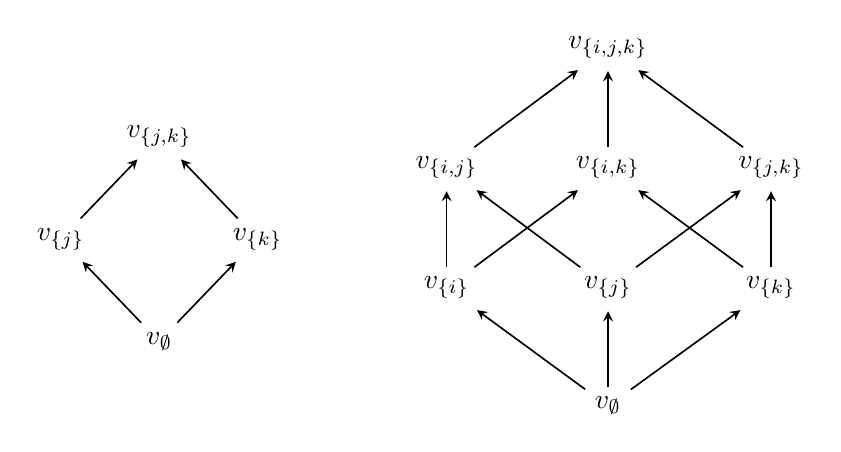
\begin{tikzpicture}
      [%node distance=1.8cm, % on grid,
        t/.style={}, % {rectangle, draw=blue!50, fill=blue!20, thick},
        p/.style={->, shorten >=1pt, >=stealth, semithick}]
      \node [t] at (0, 1.3) (jk) {$\vv_{\{j,k\}}$};
      \node [t] at (-1.25, 0) (j) {$\vv_{\{j\}}$}
      edge [p] (jk);
      \node [t] at (1.25, 0) (k) {$\vv_{\{k\}}$}
      edge [p] (jk);
      \node [t] at (0, -1.3)  {$\vv_{\emptyset}$}
      edge [p] (j) edge [p] (k);
      %
      \node [t] at (5.7, 2.43) (ijk) {$\vv_{\{i,j,k\}}$};
      \node [t] (ik) [below=of ijk] {$\vv_{\{i,k\}}$}
      edge [p] (ijk);
      \node [t] (ij) [left=of ik] {$\vv_{\{i,j\}}$}
      edge [p] (ijk);
      \node [t] (jk) [right=of ik] {$\vv_{\{j,k\}}$}
      edge [p] (ijk);
      \node [t] (i) [below=of ij] {$\vv_{\{i\}}$}
      edge [p] (ij) edge [p] (ik);
      \node [t] (j) [below=of ik] {$\vv_{\{j\}}$}
      edge [p] (ij) edge [p] (jk);
      \node [t] (k) [below=of jk] {$\vv_{\{k\}}$}
      edge [p] (ik) edge [p] (jk);
      \node [t] [below=of j] {$\vv_{\emptyset}$}
      edge [p] (i) edge [p] (j) edge [p] (k);
    \end{tikzpicture}
    \caption{Progression of the algorithm for a system of two banks and
      for a system of three.}
  \end{figure}
\end{frame}

\begin{frame}[label=supportingtheory]
  \frametitle{Some supporting theory}
  \begin{theorem}
    For survival sets $\sA$ and $\sB$,
    \begin{equation*}
      \sB\subseteq \sA\implies \vv_{\sB}\leq \vv_{\sA}.
    \end{equation*}
  \end{theorem}
  \begin{corollary}
    With $\vE^{*}(\va,\vu)$ the \alert{equity valuation function}
    indicating solvency,
    \begin{multline*}
      \text{if}\quad\exists\, \sB\subseteq \sA\quad\text{such that}\quad \forall i \in \sA \quad
      0<E^{*}_{i}(\va,\vv_{\sB}(\va))\\
      \text{then}\quad
      \forall i \in \sA\quad 0<E^{*}_{i}(\va,\vv_{\sA}(\va)).
    \end{multline*}
  \end{corollary}
\end{frame}

\subsection{Nonzero recovery rate}

\begin{frame}[label=recoveryrate]
  \frametitle{Pricing with recovery rate $\beta=0.4$}
  \hspace{\plotshift}
  \begin{tikzpicture}
    \begin{axis}[
        title={
          \begin{overprint}[132pt]
            \onslide<1>
            Bank $\one$ debt valuation
            $\val{\one}{t}$
            \onslide<2>
            Bank $\two$ debt valuation
            $\val{\two}{t}$
          \end{overprint}
        },
        xlabel={$\ass{\one}{t}$},
        ylabel={$\ass{\two}{t}$},
        xmin=1010, xmax=1120,
        ymin=720, ymax=810,
        ticklabel style={font=\small,},
        extra x ticks={1063.6},
        extra x tick labels={$\lia{\one}$},
        extra y ticks={774.8},
        extra y tick labels={$\lia{\two}$},
        width=\plotwidth,
        height=\plotheight,
      ]
      \only<1> {
        \begin{scope}[semitransparent]
          \path [draw=color0, semithick]
(axis cs:1035.02,810)
--(axis cs:1035.02,809.5)
--(axis cs:1035.02,809)
--(axis cs:1035.02,808.5)
--(axis cs:1035.02,808)
--(axis cs:1035.02,807.5)
--(axis cs:1035.02,807)
--(axis cs:1035.02,806.5)
--(axis cs:1035.02,806)
--(axis cs:1035.02,805.5)
--(axis cs:1035.02,805)
--(axis cs:1035.02,804.5)
--(axis cs:1035.02,804)
--(axis cs:1035.02,803.5)
--(axis cs:1035.02,803)
--(axis cs:1035.02,802.5)
--(axis cs:1035.02,802)
--(axis cs:1035.02,801.5)
--(axis cs:1035.02,801)
--(axis cs:1035.02,800.5)
--(axis cs:1035.02,800)
--(axis cs:1035.02,799.5)
--(axis cs:1035.02,799)
--(axis cs:1035.02,798.5)
--(axis cs:1035.02,798)
--(axis cs:1035.02,797.5)
--(axis cs:1035.02,797)
--(axis cs:1035.02,796.5)
--(axis cs:1035.02,796)
--(axis cs:1035.02,795.5)
--(axis cs:1035.02,795)
--(axis cs:1035.02,794.5)
--(axis cs:1035.02,794)
--(axis cs:1035.02,793.5)
--(axis cs:1035.02,793)
--(axis cs:1035.02,792.5)
--(axis cs:1035.02,792)
--(axis cs:1035.02,791.5)
--(axis cs:1035.02,791)
--(axis cs:1035.02,790.5)
--(axis cs:1035.02,790)
--(axis cs:1035.02,789.5)
--(axis cs:1035.02,789)
--(axis cs:1035.02,788.5)
--(axis cs:1035.02,788)
--(axis cs:1035.02,787.5)
--(axis cs:1035.02,787)
--(axis cs:1035.02,786.5)
--(axis cs:1035.02,786)
--(axis cs:1035.02,785.5)
--(axis cs:1035.02,785)
--(axis cs:1035.02,784.5)
--(axis cs:1035.02,784)
--(axis cs:1035.02,783.5)
--(axis cs:1035.02,783)
--(axis cs:1035.02,782.5)
--(axis cs:1035.02,782)
--(axis cs:1035.02,781.5)
--(axis cs:1035.02,781)
--(axis cs:1035.02,780.5)
--(axis cs:1035.02,780)
--(axis cs:1035.02,779.5)
--(axis cs:1035.02,779)
--(axis cs:1035.02,778.5)
--(axis cs:1035.02,778)
--(axis cs:1035.02,777.5)
--(axis cs:1035.02,777)
--(axis cs:1035.02,776.5)
--(axis cs:1035.02,776)
--(axis cs:1035.02,775.5)
--(axis cs:1035.02,775)
--(axis cs:1035.12311557789,774.5)
--(axis cs:1035.32046678636,774)
--(axis cs:1035.5,773.586776859504)
--(axis cs:1035.5340356564,773.5)
--(axis cs:1035.71837088388,773)
--(axis cs:1035.93016759777,772.5)
--(axis cs:1036,772.331081081081)
--(axis cs:1036.12311557789,772)
--(axis cs:1036.32046678636,771.5)
--(axis cs:1036.5,771.086776859504)
--(axis cs:1036.5340356564,771)
--(axis cs:1036.71837088388,770.5)
--(axis cs:1036.93016759777,770)
--(axis cs:1037,769.831081081081)
--(axis cs:1037.12311557789,769.5)
--(axis cs:1037.32046678636,769)
--(axis cs:1037.5,768.586776859504)
--(axis cs:1037.5340356564,768.5)
--(axis cs:1037.71837088388,768)
--(axis cs:1037.93016759777,767.5)
--(axis cs:1038,767.331081081081)
--(axis cs:1038.12311557789,767)
--(axis cs:1038.32046678636,766.5)
--(axis cs:1038.5,766.086776859504)
--(axis cs:1038.5340356564,766)
--(axis cs:1038.71837088388,765.5)
--(axis cs:1038.93016759777,765)
--(axis cs:1039,764.831081081081)
--(axis cs:1039.12311557789,764.5)
--(axis cs:1039.32046678636,764)
--(axis cs:1039.5,763.586776859504)
--(axis cs:1039.5340356564,763.5)
--(axis cs:1039.71837088388,763)
--(axis cs:1039.93016759777,762.5)
--(axis cs:1040,762.331081081081)
--(axis cs:1040.12311557789,762)
--(axis cs:1040.32046678636,761.5)
--(axis cs:1040.5,761.086776859504)
--(axis cs:1040.5340356564,761)
--(axis cs:1040.71837088388,760.5)
--(axis cs:1040.93016759777,760)
--(axis cs:1041,759.831081081081)
--(axis cs:1041.12311557789,759.5)
--(axis cs:1041.32046678636,759)
--(axis cs:1041.5,758.586776859504)
--(axis cs:1041.5340356564,758.5)
--(axis cs:1041.71837088388,758)
--(axis cs:1041.93016759777,757.5)
--(axis cs:1042,757.331081081081)
--(axis cs:1042.12311557789,757)
--(axis cs:1042.32046678636,756.5)
--(axis cs:1042.5,756.086776859504)
--(axis cs:1042.5340356564,756)
--(axis cs:1042.71837088388,755.5)
--(axis cs:1042.93016759777,755)
--(axis cs:1043,754.831081081081)
--(axis cs:1043.12311557789,754.5)
--(axis cs:1043.32046678636,754)
--(axis cs:1043.5,753.586776859504)
--(axis cs:1043.5340356564,753.5)
--(axis cs:1043.71837088388,753)
--(axis cs:1043.93016759777,752.5)
--(axis cs:1044,752.331081081081)
--(axis cs:1044.12311557789,752)
--(axis cs:1044.32046678636,751.5)
--(axis cs:1044.5,751.086776859504)
--(axis cs:1044.5340356564,751)
--(axis cs:1044.71837088388,750.5)
--(axis cs:1044.93016759777,750)
--(axis cs:1045,749.831081081081)
--(axis cs:1045.12311557789,749.5)
--(axis cs:1045.32046678636,749)
--(axis cs:1045.5,748.586776859504)
--(axis cs:1045.5340356564,748.5)
--(axis cs:1045.71837088388,748)
--(axis cs:1045.93016759777,747.5)
--(axis cs:1046,747.331081081081)
--(axis cs:1046.12311557789,747)
--(axis cs:1046.32046678636,746.5)
--(axis cs:1046.5,746.086776859504)
--(axis cs:1046.5340356564,746)
--(axis cs:1046.71837088388,745.5)
--(axis cs:1046.93016759777,745)
--(axis cs:1047,744.831081081081)
--(axis cs:1047.12311557789,744.5)
--(axis cs:1047.32046678636,744)
--(axis cs:1047.5,743.586776859504)
--(axis cs:1047.5340356564,743.5)
--(axis cs:1047.71837088388,743)
--(axis cs:1047.93016759777,742.5)
--(axis cs:1048,742.331081081081)
--(axis cs:1048.12311557789,742)
--(axis cs:1048.32046678636,741.5)
--(axis cs:1048.5,741.086776859504)
--(axis cs:1048.5340356564,741)
--(axis cs:1048.71837088388,740.5)
--(axis cs:1048.93016759777,740)
--(axis cs:1049,739.831081081081)
--(axis cs:1049.12311557789,739.5)
--(axis cs:1049.32046678636,739)
--(axis cs:1049.5,738.5)
--(axis cs:1049.5,738)
--(axis cs:1049.5,737.5)
--(axis cs:1049.5,737)
--(axis cs:1049.5,736.5)
--(axis cs:1049.5,736)
--(axis cs:1049.5,735.5)
--(axis cs:1049.5,735)
--(axis cs:1049.5,734.5)
--(axis cs:1049.5,734)
--(axis cs:1049.5,733.5)
--(axis cs:1049.5,733)
--(axis cs:1049.5,732.5)
--(axis cs:1049.5,732)
--(axis cs:1049.5,731.5)
--(axis cs:1049.5,731)
--(axis cs:1049.5,730.5)
--(axis cs:1049.5,730)
--(axis cs:1049.5,729.5)
--(axis cs:1049.5,729)
--(axis cs:1049.5,728.5)
--(axis cs:1049.5,728)
--(axis cs:1049.5,727.5)
--(axis cs:1049.5,727)
--(axis cs:1049.5,726.5)
--(axis cs:1049.5,726)
--(axis cs:1049.5,725.5)
--(axis cs:1049.5,725)
--(axis cs:1049.5,724.5)
--(axis cs:1049.5,724)
--(axis cs:1049.5,723.5)
--(axis cs:1049.5,723)
--(axis cs:1049.5,722.5)
--(axis cs:1049.5,722)
--(axis cs:1049.5,721.5)
--(axis cs:1049.5,721)
--(axis cs:1049.5,720.5)
--(axis cs:1049.5,720);

\path [draw=color1, semithick]
(axis cs:1042.07,810)
--(axis cs:1042.07,809.5)
--(axis cs:1042.07,809)
--(axis cs:1042.07,808.5)
--(axis cs:1042.07,808)
--(axis cs:1042.07,807.5)
--(axis cs:1042.07,807)
--(axis cs:1042.07,806.5)
--(axis cs:1042.07,806)
--(axis cs:1042.07,805.5)
--(axis cs:1042.07,805)
--(axis cs:1042.07,804.5)
--(axis cs:1042.07,804)
--(axis cs:1042.07,803.5)
--(axis cs:1042.07,803)
--(axis cs:1042.07,802.5)
--(axis cs:1042.07,802)
--(axis cs:1042.07,801.5)
--(axis cs:1042.07,801)
--(axis cs:1042.07,800.5)
--(axis cs:1042.07,800)
--(axis cs:1042.07,799.5)
--(axis cs:1042.07,799)
--(axis cs:1042.07,798.5)
--(axis cs:1042.07,798)
--(axis cs:1042.07,797.5)
--(axis cs:1042.07,797)
--(axis cs:1042.07,796.5)
--(axis cs:1042.07,796)
--(axis cs:1042.07,795.5)
--(axis cs:1042.07,795)
--(axis cs:1042.07,794.5)
--(axis cs:1042.07,794)
--(axis cs:1042.07,793.5)
--(axis cs:1042.07,793)
--(axis cs:1042.07,792.5)
--(axis cs:1042.07,792)
--(axis cs:1042.07,791.5)
--(axis cs:1042.07,791)
--(axis cs:1042.07,790.5)
--(axis cs:1042.07,790)
--(axis cs:1042.07,789.5)
--(axis cs:1042.07,789)
--(axis cs:1042.07,788.5)
--(axis cs:1042.07,788)
--(axis cs:1042.07,787.5)
--(axis cs:1042.07,787)
--(axis cs:1042.07,786.5)
--(axis cs:1042.07,786)
--(axis cs:1042.07,785.5)
--(axis cs:1042.07,785)
--(axis cs:1042.07,784.5)
--(axis cs:1042.07,784)
--(axis cs:1042.07,783.5)
--(axis cs:1042.07,783)
--(axis cs:1042.07,782.5)
--(axis cs:1042.07,782)
--(axis cs:1042.07,781.5)
--(axis cs:1042.07,781)
--(axis cs:1042.07,780.5)
--(axis cs:1042.07,780)
--(axis cs:1042.07,779.5)
--(axis cs:1042.07,779)
--(axis cs:1042.07,778.5)
--(axis cs:1042.07,778)
--(axis cs:1042.07,777.5)
--(axis cs:1042.07,777)
--(axis cs:1042.07,776.5)
--(axis cs:1042.07,776)
--(axis cs:1042.07,775.5)
--(axis cs:1042.07,775)
--(axis cs:1042.07,774.5)
--(axis cs:1042.07,774)
--(axis cs:1042.07,773.5)
--(axis cs:1042.07,773)
--(axis cs:1042.07,772.5)
--(axis cs:1042.07325141777,772)
--(axis cs:1042.262,771.5)
--(axis cs:1042.462,771)
--(axis cs:1042.5,770.905)
--(axis cs:1042.662,770.5)
--(axis cs:1042.862,770)
--(axis cs:1043,769.655)
--(axis cs:1043.062,769.5)
--(axis cs:1043.262,769)
--(axis cs:1043.462,768.5)
--(axis cs:1043.5,768.405)
--(axis cs:1043.662,768)
--(axis cs:1043.862,767.5)
--(axis cs:1044,767.155)
--(axis cs:1044.062,767)
--(axis cs:1044.262,766.5)
--(axis cs:1044.462,766)
--(axis cs:1044.5,765.905)
--(axis cs:1044.662,765.5)
--(axis cs:1044.862,765)
--(axis cs:1045,764.655)
--(axis cs:1045.062,764.5)
--(axis cs:1045.262,764)
--(axis cs:1045.462,763.5)
--(axis cs:1045.5,763.405)
--(axis cs:1045.662,763)
--(axis cs:1045.862,762.5)
--(axis cs:1046,762.155)
--(axis cs:1046.062,762)
--(axis cs:1046.262,761.5)
--(axis cs:1046.462,761)
--(axis cs:1046.5,760.905)
--(axis cs:1046.662,760.5)
--(axis cs:1046.862,760)
--(axis cs:1047,759.655)
--(axis cs:1047.062,759.5)
--(axis cs:1047.262,759)
--(axis cs:1047.462,758.5)
--(axis cs:1047.5,758.405)
--(axis cs:1047.662,758)
--(axis cs:1047.862,757.5)
--(axis cs:1048,757.155)
--(axis cs:1048.062,757)
--(axis cs:1048.262,756.5)
--(axis cs:1048.462,756)
--(axis cs:1048.5,755.905)
--(axis cs:1048.662,755.5)
--(axis cs:1048.862,755)
--(axis cs:1049,754.655)
--(axis cs:1049.062,754.5)
--(axis cs:1049.262,754)
--(axis cs:1049.462,753.5)
--(axis cs:1049.5,753.405)
--(axis cs:1049.662,753)
--(axis cs:1049.862,752.5)
--(axis cs:1050,752.155)
--(axis cs:1050.062,752)
--(axis cs:1050.262,751.5)
--(axis cs:1050.462,751)
--(axis cs:1050.5,750.905)
--(axis cs:1050.662,750.5)
--(axis cs:1050.862,750)
--(axis cs:1051,749.655)
--(axis cs:1051.062,749.5)
--(axis cs:1051.262,749)
--(axis cs:1051.462,748.5)
--(axis cs:1051.5,748.405)
--(axis cs:1051.662,748)
--(axis cs:1051.862,747.5)
--(axis cs:1052,747.155)
--(axis cs:1052.062,747)
--(axis cs:1052.262,746.5)
--(axis cs:1052.462,746)
--(axis cs:1052.5,745.905)
--(axis cs:1052.662,745.5)
--(axis cs:1052.862,745)
--(axis cs:1053,744.655)
--(axis cs:1053.062,744.5)
--(axis cs:1053.262,744)
--(axis cs:1053.462,743.5)
--(axis cs:1053.5,743.405)
--(axis cs:1053.662,743)
--(axis cs:1053.862,742.5)
--(axis cs:1054,742.155)
--(axis cs:1054.062,742)
--(axis cs:1054.262,741.5)
--(axis cs:1054.462,741)
--(axis cs:1054.5,740.905)
--(axis cs:1054.662,740.5)
--(axis cs:1054.862,740)
--(axis cs:1055,739.655)
--(axis cs:1055.062,739.5)
--(axis cs:1055.262,739)
--(axis cs:1055.462,738.5)
--(axis cs:1055.5,738.405)
--(axis cs:1055.662,738)
--(axis cs:1055.862,737.5)
--(axis cs:1056,737.155)
--(axis cs:1056.062,737)
--(axis cs:1056.262,736.5)
--(axis cs:1056.462,736)
--(axis cs:1056.5,735.7625)
--(axis cs:1056.55,735.5)
--(axis cs:1056.55,735)
--(axis cs:1056.55,734.5)
--(axis cs:1056.55,734)
--(axis cs:1056.55,733.5)
--(axis cs:1056.55,733)
--(axis cs:1056.55,732.5)
--(axis cs:1056.55,732)
--(axis cs:1056.55,731.5)
--(axis cs:1056.55,731)
--(axis cs:1056.55,730.5)
--(axis cs:1056.55,730)
--(axis cs:1056.55,729.5)
--(axis cs:1056.55,729)
--(axis cs:1056.55,728.5)
--(axis cs:1056.55,728)
--(axis cs:1056.55,727.5)
--(axis cs:1056.55,727)
--(axis cs:1056.55,726.5)
--(axis cs:1056.55,726)
--(axis cs:1056.55,725.5)
--(axis cs:1056.55,725)
--(axis cs:1056.55,724.5)
--(axis cs:1056.55,724)
--(axis cs:1056.55,723.5)
--(axis cs:1056.55,723)
--(axis cs:1056.55,722.5)
--(axis cs:1056.55,722)
--(axis cs:1056.55,721.5)
--(axis cs:1056.55,721)
--(axis cs:1056.55,720.5)
--(axis cs:1056.55,720);

\path [draw=color2, semithick]
(axis cs:1049.12,810)
--(axis cs:1049.12,809.5)
--(axis cs:1049.12,809)
--(axis cs:1049.12,808.5)
--(axis cs:1049.12,808)
--(axis cs:1049.12,807.5)
--(axis cs:1049.12,807)
--(axis cs:1049.12,806.5)
--(axis cs:1049.12,806)
--(axis cs:1049.12,805.5)
--(axis cs:1049.12,805)
--(axis cs:1049.12,804.5)
--(axis cs:1049.12,804)
--(axis cs:1049.12,803.5)
--(axis cs:1049.12,803)
--(axis cs:1049.12,802.5)
--(axis cs:1049.12,802)
--(axis cs:1049.12,801.5)
--(axis cs:1049.12,801)
--(axis cs:1049.12,800.5)
--(axis cs:1049.12,800)
--(axis cs:1049.12,799.5)
--(axis cs:1049.12,799)
--(axis cs:1049.12,798.5)
--(axis cs:1049.12,798)
--(axis cs:1049.12,797.5)
--(axis cs:1049.12,797)
--(axis cs:1049.12,796.5)
--(axis cs:1049.12,796)
--(axis cs:1049.12,795.5)
--(axis cs:1049.12,795)
--(axis cs:1049.12,794.5)
--(axis cs:1049.12,794)
--(axis cs:1049.12,793.5)
--(axis cs:1049.12,793)
--(axis cs:1049.12,792.5)
--(axis cs:1049.12,792)
--(axis cs:1049.12,791.5)
--(axis cs:1049.12,791)
--(axis cs:1049.12,790.5)
--(axis cs:1049.12,790)
--(axis cs:1049.12,789.5)
--(axis cs:1049.12,789)
--(axis cs:1049.12,788.5)
--(axis cs:1049.12,788)
--(axis cs:1049.12,787.5)
--(axis cs:1049.12,787)
--(axis cs:1049.12,786.5)
--(axis cs:1049.12,786)
--(axis cs:1049.12,785.5)
--(axis cs:1049.12,785)
--(axis cs:1049.12,784.5)
--(axis cs:1049.12,784)
--(axis cs:1049.12,783.5)
--(axis cs:1049.12,783)
--(axis cs:1049.12,782.5)
--(axis cs:1049.12,782)
--(axis cs:1049.12,781.5)
--(axis cs:1049.12,781)
--(axis cs:1049.12,780.5)
--(axis cs:1049.12,780)
--(axis cs:1049.12,779.5)
--(axis cs:1049.12,779)
--(axis cs:1049.12,778.5)
--(axis cs:1049.12,778)
--(axis cs:1049.12,777.5)
--(axis cs:1049.12,777)
--(axis cs:1049.12,776.5)
--(axis cs:1049.12,776)
--(axis cs:1049.12,775.5)
--(axis cs:1049.12,775)
--(axis cs:1049.12,774.5)
--(axis cs:1049.12,774)
--(axis cs:1049.12,773.5)
--(axis cs:1049.12,773)
--(axis cs:1049.12,772.5)
--(axis cs:1049.12,772)
--(axis cs:1049.12,771.5)
--(axis cs:1049.12,771)
--(axis cs:1049.12,770.5)
--(axis cs:1049.12,770)
--(axis cs:1049.12,769.5)
--(axis cs:1049.2046991812,769)
--(axis cs:1049.39880358923,768.5)
--(axis cs:1049.5,768.231481481481)
--(axis cs:1049.59689922481,768)
--(axis cs:1049.80508765899,767.5)
--(axis cs:1049.98649083307,767)
--(axis cs:1050,766.965964343598)
--(axis cs:1050.2046991812,766.5)
--(axis cs:1050.39880358923,766)
--(axis cs:1050.5,765.731481481481)
--(axis cs:1050.59689922481,765.5)
--(axis cs:1050.80508765899,765)
--(axis cs:1050.98649083307,764.5)
--(axis cs:1051,764.465964343598)
--(axis cs:1051.2046991812,764)
--(axis cs:1051.39880358923,763.5)
--(axis cs:1051.5,763.231481481481)
--(axis cs:1051.59689922481,763)
--(axis cs:1051.80508765899,762.5)
--(axis cs:1051.98649083307,762)
--(axis cs:1052,761.965964343598)
--(axis cs:1052.2046991812,761.5)
--(axis cs:1052.39880358923,761)
--(axis cs:1052.5,760.731481481481)
--(axis cs:1052.59689922481,760.5)
--(axis cs:1052.80508765899,760)
--(axis cs:1052.98649083307,759.5)
--(axis cs:1053,759.465964343598)
--(axis cs:1053.2046991812,759)
--(axis cs:1053.39880358923,758.5)
--(axis cs:1053.5,758.231481481481)
--(axis cs:1053.59689922481,758)
--(axis cs:1053.80508765899,757.5)
--(axis cs:1053.98649083307,757)
--(axis cs:1054,756.965964343598)
--(axis cs:1054.2046991812,756.5)
--(axis cs:1054.39880358923,756)
--(axis cs:1054.5,755.731481481481)
--(axis cs:1054.59689922481,755.5)
--(axis cs:1054.80508765899,755)
--(axis cs:1054.98649083307,754.5)
--(axis cs:1055,754.465964343598)
--(axis cs:1055.2046991812,754)
--(axis cs:1055.39880358923,753.5)
--(axis cs:1055.5,753.231481481481)
--(axis cs:1055.59689922481,753)
--(axis cs:1055.80508765899,752.5)
--(axis cs:1055.98649083307,752)
--(axis cs:1056,751.965964343598)
--(axis cs:1056.2046991812,751.5)
--(axis cs:1056.39880358923,751)
--(axis cs:1056.5,750.731481481481)
--(axis cs:1056.59689922481,750.5)
--(axis cs:1056.80508765899,750)
--(axis cs:1056.98649083307,749.5)
--(axis cs:1057,749.465964343598)
--(axis cs:1057.2046991812,749)
--(axis cs:1057.39880358923,748.5)
--(axis cs:1057.5,748.231481481481)
--(axis cs:1057.59689922481,748)
--(axis cs:1057.80508765899,747.5)
--(axis cs:1057.98649083307,747)
--(axis cs:1058,746.965964343598)
--(axis cs:1058.2046991812,746.5)
--(axis cs:1058.39880358923,746)
--(axis cs:1058.5,745.731481481481)
--(axis cs:1058.59689922481,745.5)
--(axis cs:1058.80508765899,745)
--(axis cs:1058.98649083307,744.5)
--(axis cs:1059,744.465964343598)
--(axis cs:1059.2046991812,744)
--(axis cs:1059.39880358923,743.5)
--(axis cs:1059.5,743.231481481481)
--(axis cs:1059.59689922481,743)
--(axis cs:1059.80508765899,742.5)
--(axis cs:1059.98649083307,742)
--(axis cs:1060,741.965964343598)
--(axis cs:1060.2046991812,741.5)
--(axis cs:1060.39880358923,741)
--(axis cs:1060.5,740.731481481481)
--(axis cs:1060.59689922481,740.5)
--(axis cs:1060.80508765899,740)
--(axis cs:1060.98649083307,739.5)
--(axis cs:1061,739.465964343598)
--(axis cs:1061.2046991812,739)
--(axis cs:1061.39880358923,738.5)
--(axis cs:1061.5,738.231481481481)
--(axis cs:1061.59689922481,738)
--(axis cs:1061.80508765899,737.5)
--(axis cs:1061.98649083307,737)
--(axis cs:1062,736.965964343598)
--(axis cs:1062.2046991812,736.5)
--(axis cs:1062.39880358923,736)
--(axis cs:1062.5,735.731481481481)
--(axis cs:1062.59689922481,735.5)
--(axis cs:1062.80508765899,735)
--(axis cs:1062.98649083307,734.5)
--(axis cs:1063,734.465964343598)
--(axis cs:1063.2046991812,734)
--(axis cs:1063.39880358923,733.5)
--(axis cs:1063.5,733.231481481481)
--(axis cs:1063.59689922481,733)
--(axis cs:1063.6,732.5)
--(axis cs:1063.6,732)
--(axis cs:1063.6,731.5)
--(axis cs:1063.6,731)
--(axis cs:1063.6,730.5)
--(axis cs:1063.6,730)
--(axis cs:1063.6,729.5)
--(axis cs:1063.6,729)
--(axis cs:1063.6,728.5)
--(axis cs:1063.6,728)
--(axis cs:1063.6,727.5)
--(axis cs:1063.6,727)
--(axis cs:1063.6,726.5)
--(axis cs:1063.6,726)
--(axis cs:1063.6,725.5)
--(axis cs:1063.6,725)
--(axis cs:1063.6,724.5)
--(axis cs:1063.6,724)
--(axis cs:1063.6,723.5)
--(axis cs:1063.6,723)
--(axis cs:1063.6,722.5)
--(axis cs:1063.6,722)
--(axis cs:1063.6,721.5)
--(axis cs:1063.6,721)
--(axis cs:1063.6,720.5)
--(axis cs:1063.6,720);

\path [draw=color3, semithick]
(axis cs:1052.80800936985,810)
--(axis cs:1052.81042877094,809.5)
--(axis cs:1052.75977490266,809)
--(axis cs:1052.8224883217,808.5)
--(axis cs:1052.79394409563,808)
--(axis cs:1052.78103654986,807.5)
--(axis cs:1052.83356259266,807)
--(axis cs:1052.8143934908,806.5)
--(axis cs:1052.8256925255,806)
--(axis cs:1052.78457225219,805.5)
--(axis cs:1052.74329027991,805)
--(axis cs:1052.80785421146,804.5)
--(axis cs:1052.78592891187,804)
--(axis cs:1052.78686593594,803.5)
--(axis cs:1052.77754627942,803)
--(axis cs:1052.81297937798,802.5)
--(axis cs:1052.79570104771,802)
--(axis cs:1052.78132726446,801.5)
--(axis cs:1052.82454254642,801)
--(axis cs:1052.82408728714,800.5)
--(axis cs:1052.795310193,800)
--(axis cs:1052.79787010987,799.5)
--(axis cs:1052.81132608734,799)
--(axis cs:1052.75976383952,798.5)
--(axis cs:1052.79737291668,798)
--(axis cs:1052.82576187053,797.5)
--(axis cs:1052.74835944341,797)
--(axis cs:1052.77201783509,796.5)
--(axis cs:1052.76057214665,796)
--(axis cs:1052.80496792501,795.5)
--(axis cs:1052.82203567531,795)
--(axis cs:1052.75428951865,794.5)
--(axis cs:1052.78484775343,794)
--(axis cs:1052.80076047554,793.5)
--(axis cs:1052.77538528691,793)
--(axis cs:1052.75400301849,792.5)
--(axis cs:1052.7757871477,792)
--(axis cs:1052.77594176327,791.5)
--(axis cs:1052.81393188884,791)
--(axis cs:1052.83163365757,790.5)
--(axis cs:1052.77421439678,790)
--(axis cs:1052.81675439749,789.5)
--(axis cs:1052.80028675467,789)
--(axis cs:1052.78825503577,788.5)
--(axis cs:1052.81951899655,788)
--(axis cs:1052.81466058217,787.5)
--(axis cs:1052.74608147788,787)
--(axis cs:1052.78564603419,786.5)
--(axis cs:1052.81583993544,786)
--(axis cs:1052.76235907997,785.5)
--(axis cs:1052.80047231518,785)
--(axis cs:1052.76614098235,784.5)
--(axis cs:1052.76989698465,784)
--(axis cs:1052.83246240343,783.5)
--(axis cs:1052.77602900689,783)
--(axis cs:1052.77851785304,782.5)
--(axis cs:1052.80265363182,782)
--(axis cs:1052.80037701997,781.5)
--(axis cs:1052.80335403816,781)
--(axis cs:1052.79424499819,780.5)
--(axis cs:1052.78304742133,780)
--(axis cs:1052.83861818026,779.5)
--(axis cs:1052.7956191484,779)
--(axis cs:1052.78048472627,778.5)
--(axis cs:1052.79038757628,778)
--(axis cs:1052.8234972649,777.5)
--(axis cs:1052.78990532698,777)
--(axis cs:1052.82406317785,776.5)
--(axis cs:1052.79685908387,776)
--(axis cs:1052.81607314653,775.5)
--(axis cs:1052.78177149231,775)
--(axis cs:1052.84357345094,774.5)
--(axis cs:1052.81112962951,774)
--(axis cs:1052.80653872613,773.5)
--(axis cs:1052.83048293663,773)
--(axis cs:1052.86511723021,772.5)
--(axis cs:1052.8449105908,772)
--(axis cs:1052.89333834116,771.5)
--(axis cs:1052.90592417859,771)
--(axis cs:1052.96511559656,770.5)
--(axis cs:1052.97923579392,770)
--(axis cs:1053,769.804248732513)
--(axis cs:1053.04143693182,769.5)
--(axis cs:1053.21781506646,769)
--(axis cs:1053.30146969367,768.5)
--(axis cs:1053.5,768.06155818965)
--(axis cs:1053.52590695664,768)
--(axis cs:1053.67409450907,767.5)
--(axis cs:1053.89558127703,767)
--(axis cs:1054,766.721429768091)
--(axis cs:1054.08747682262,766.5)
--(axis cs:1054.24864719671,766)
--(axis cs:1054.43354532097,765.5)
--(axis cs:1054.5,765.319425967285)
--(axis cs:1054.61151869081,765)
--(axis cs:1054.83629516714,764.5)
--(axis cs:1055,764.027962347897)
--(axis cs:1055.00776182121,764)
--(axis cs:1055.21023436512,763.5)
--(axis cs:1055.40841333787,763)
--(axis cs:1055.5,762.746436277142)
--(axis cs:1055.59545403138,762.5)
--(axis cs:1055.77691031483,762)
--(axis cs:1055.95707322992,761.5)
--(axis cs:1056,761.405039625076)
--(axis cs:1056.18098560798,761)
--(axis cs:1056.4239599763,760.5)
--(axis cs:1056.5,760.149691893487)
--(axis cs:1056.53867832569,760)
--(axis cs:1056.79950572358,759.5)
--(axis cs:1056.97807145217,759)
--(axis cs:1057,758.951131773776)
--(axis cs:1057.18750638733,758.5)
--(axis cs:1057.39217865732,758)
--(axis cs:1057.5,757.702875354626)
--(axis cs:1057.57531819119,757.5)
--(axis cs:1057.7754441526,757)
--(axis cs:1058,756.516939449454)
--(axis cs:1058.00930159607,756.5)
--(axis cs:1058.21439200022,756)
--(axis cs:1058.40912005458,755.5)
--(axis cs:1058.5,755.265100223623)
--(axis cs:1058.59692196764,755)
--(axis cs:1058.83588587401,754.5)
--(axis cs:1059,754.098537660768)
--(axis cs:1059.04183432409,754)
--(axis cs:1059.19415401243,753.5)
--(axis cs:1059.3958454398,753)
--(axis cs:1059.5,752.723092848698)
--(axis cs:1059.58142304232,752.5)
--(axis cs:1059.79277446863,752)
--(axis cs:1059.99992019549,751.5)
--(axis cs:1060,751.499799521981)
--(axis cs:1060.24331531186,751)
--(axis cs:1060.40288292907,750.5)
--(axis cs:1060.5,750.136493729575)
--(axis cs:1060.5413793249,750)
--(axis cs:1060.81308670765,749.5)
--(axis cs:1060.96231187897,749)
--(axis cs:1061,748.920732783713)
--(axis cs:1061.20477407058,748.5)
--(axis cs:1061.39162224134,748)
--(axis cs:1061.5,747.757639300678)
--(axis cs:1061.61673594158,747.5)
--(axis cs:1061.77523087759,747)
--(axis cs:1061.98924548057,746.5)
--(axis cs:1062,746.477214813037)
--(axis cs:1062.2197750237,746)
--(axis cs:1062.40650813956,745.5)
--(axis cs:1062.5,745.295163741859)
--(axis cs:1062.62303048895,745)
--(axis cs:1062.81564774493,744.5)
--(axis cs:1063,744.007038180233)
--(axis cs:1063.00252996259,744)
--(axis cs:1063.19832818475,743.5)
--(axis cs:1063.41256879824,743)
--(axis cs:1063.5,742.783199954174)
--(axis cs:1063.60464308194,742.5)
--(axis cs:1063.8641621935,742)
--(axis cs:1064,741.61616687409)
--(axis cs:1064.02919153171,741.5)
--(axis cs:1064.17448745245,741)
--(axis cs:1064.41852767906,740.5)
--(axis cs:1064.5,740.31416899809)
--(axis cs:1064.64052611163,740)
--(axis cs:1064.80762018711,739.5)
--(axis cs:1064.98501570268,739)
--(axis cs:1065,738.967936430122)
--(axis cs:1065.19605677317,738.5)
--(axis cs:1065.42290018944,738)
--(axis cs:1065.5,737.795361561578)
--(axis cs:1065.59877615756,737.5)
--(axis cs:1065.81459016655,737)
--(axis cs:1065.95893264098,736.5)
--(axis cs:1066,736.315264022898)
--(axis cs:1066.0801243839,736)
--(axis cs:1066.31004652614,735.5)
--(axis cs:1066.5,735.129250453967)
--(axis cs:1066.57118697751,735)
--(axis cs:1066.71724280056,734.5)
--(axis cs:1066.8571082901,734)
--(axis cs:1066.98738313207,733.5)
--(axis cs:1067,733.436740401516)
--(axis cs:1067.0851533869,733)
--(axis cs:1067.13524516234,732.5)
--(axis cs:1067.2141038792,732)
--(axis cs:1067.29140977489,731.5)
--(axis cs:1067.29095119249,731)
--(axis cs:1067.26210770518,730.5)
--(axis cs:1067.29448067837,730)
--(axis cs:1067.3086219542,729.5)
--(axis cs:1067.31673404714,729)
--(axis cs:1067.29796691638,728.5)
--(axis cs:1067.29177730804,728)
--(axis cs:1067.32335563919,727.5)
--(axis cs:1067.30456508929,727)
--(axis cs:1067.35261755966,726.5)
--(axis cs:1067.32910218635,726)
--(axis cs:1067.32307725966,725.5)
--(axis cs:1067.32142709098,725)
--(axis cs:1067.33041943707,724.5)
--(axis cs:1067.32008461376,724)
--(axis cs:1067.33242741686,723.5)
--(axis cs:1067.32171320805,723)
--(axis cs:1067.29676934284,722.5)
--(axis cs:1067.28593444517,722)
--(axis cs:1067.33521098729,721.5)
--(axis cs:1067.3349666691,721)
--(axis cs:1067.37496508803,720.5)
--(axis cs:1067.36010683471,720);

\path [draw=color4, semithick]
(axis cs:1059.56001886311,810)
--(axis cs:1059.56006499508,809.5)
--(axis cs:1059.57281796511,809)
--(axis cs:1059.5847711463,808.5)
--(axis cs:1059.5,808.165662636022)
--(axis cs:1059.46992797149,808)
--(axis cs:1059.5,807.680651293419)
--(axis cs:1059.52275484974,807.5)
--(axis cs:1059.5,807.299322457618)
--(axis cs:1059.47523934177,807)
--(axis cs:1059.5,806.787986792574)
--(axis cs:1059.54328430267,806.5)
--(axis cs:1059.5,806.186776367967)
--(axis cs:1059.47737463799,806)
--(axis cs:1059.5,805.933843288796)
--(axis cs:1059.6455458864,805.5)
--(axis cs:1059.61012182041,805)
--(axis cs:1059.5,804.562155077784)
--(axis cs:1059.48771562231,804.5)
--(axis cs:1059.5,804.38886325075)
--(axis cs:1059.55196632702,804)
--(axis cs:1059.60631675861,803.5)
--(axis cs:1059.5,803.041416205905)
--(axis cs:1059.48914463396,803)
--(axis cs:1059.4324402672,802.5)
--(axis cs:1059.5,802.19232951573)
--(axis cs:1059.55322548442,802)
--(axis cs:1059.52571680273,801.5)
--(axis cs:1059.5,801.155410703735)
--(axis cs:1059.49141124036,801)
--(axis cs:1059.49198791683,800.5)
--(axis cs:1059.5,800.452622526506)
--(axis cs:1059.5974927566,800)
--(axis cs:1059.56667861323,799.5)
--(axis cs:1059.59469252938,799)
--(axis cs:1059.5,798.602517190686)
--(axis cs:1059.47680859327,798.5)
--(axis cs:1059.5,798.243308676238)
--(axis cs:1059.52537520949,798)
--(axis cs:1059.63925695864,797.5)
--(axis cs:1059.5,797.031460230282)
--(axis cs:1059.49094864832,797)
--(axis cs:1059.5,796.951219486862)
--(axis cs:1059.59504972542,796.5)
--(axis cs:1059.5,796.10842027082)
--(axis cs:1059.47550360298,796)
--(axis cs:1059.5,795.883426891961)
--(axis cs:1059.58856078502,795.5)
--(axis cs:1059.5,795.126915398271)
--(axis cs:1059.47309887998,795)
--(axis cs:1059.49077838918,794.5)
--(axis cs:1059.5,794.340375186125)
--(axis cs:1059.52736186615,794)
--(axis cs:1059.53693895819,793.5)
--(axis cs:1059.53967290432,793)
--(axis cs:1059.5,792.734251624092)
--(axis cs:1059.47307413015,792.5)
--(axis cs:1059.5,792.283153123695)
--(axis cs:1059.54192598883,792)
--(axis cs:1059.56864122851,791.5)
--(axis cs:1059.57986142481,791)
--(axis cs:1059.5,790.731178436985)
--(axis cs:1059.44821076968,790.5)
--(axis cs:1059.5,790.294639017469)
--(axis cs:1059.58050101425,790)
--(axis cs:1059.60974271584,789.5)
--(axis cs:1059.54769570904,789)
--(axis cs:1059.5,788.584341014568)
--(axis cs:1059.49295199573,788.5)
--(axis cs:1059.5,788.399177005153)
--(axis cs:1059.54011282949,788)
--(axis cs:1059.52475929802,787.5)
--(axis cs:1059.5,787.258214981763)
--(axis cs:1059.47602019923,787)
--(axis cs:1059.5,786.728948099532)
--(axis cs:1059.52573103699,786.5)
--(axis cs:1059.532562481,786)
--(axis cs:1059.5254790115,785.5)
--(axis cs:1059.60327498565,785)
--(axis cs:1059.5,784.674160344509)
--(axis cs:1059.44072741739,784.5)
--(axis cs:1059.5,784.19784393872)
--(axis cs:1059.54457949796,784)
--(axis cs:1059.51900892042,783.5)
--(axis cs:1059.5529066598,783)
--(axis cs:1059.5872236569,782.5)
--(axis cs:1059.5,782.031534089407)
--(axis cs:1059.49490961867,782)
--(axis cs:1059.5,781.872349391943)
--(axis cs:1059.51984928536,781.5)
--(axis cs:1059.56344191204,781)
--(axis cs:1059.56160530455,780.5)
--(axis cs:1059.53307123259,780)
--(axis cs:1059.5,779.84363730163)
--(axis cs:1059.44907431511,779.5)
--(axis cs:1059.5,779.304504284333)
--(axis cs:1059.59273055035,779)
--(axis cs:1059.5,778.708221556549)
--(axis cs:1059.43735827484,778.5)
--(axis cs:1059.5,778.181043989279)
--(axis cs:1059.53995743807,778)
--(axis cs:1059.53000130686,777.5)
--(axis cs:1059.60035755697,777)
--(axis cs:1059.55625845575,776.5)
--(axis cs:1059.52481140664,776)
--(axis cs:1059.5805482229,775.5)
--(axis cs:1059.53302455562,775)
--(axis cs:1059.63428813123,774.5)
--(axis cs:1059.62024009333,774)
--(axis cs:1059.70978610002,773.5)
--(axis cs:1059.69591923824,773)
--(axis cs:1059.729592579,772.5)
--(axis cs:1059.73342018778,772)
--(axis cs:1059.83289552409,771.5)
--(axis cs:1059.93072817989,771)
--(axis cs:1059.98024359756,770.5)
--(axis cs:1060,770.324042516142)
--(axis cs:1060.04882195649,770)
--(axis cs:1060.14300633376,769.5)
--(axis cs:1060.2962108462,769)
--(axis cs:1060.40863478537,768.5)
--(axis cs:1060.5,768.296076702398)
--(axis cs:1060.6085202701,768)
--(axis cs:1060.77269214126,767.5)
--(axis cs:1060.91699507577,767)
--(axis cs:1061,766.710120025307)
--(axis cs:1061.06642868833,766.5)
--(axis cs:1061.26220233056,766)
--(axis cs:1061.47183996056,765.5)
--(axis cs:1061.5,765.406774785635)
--(axis cs:1061.61103670317,765)
--(axis cs:1061.82330565495,764.5)
--(axis cs:1061.94907934687,764)
--(axis cs:1062,763.879778865335)
--(axis cs:1062.20421836976,763.5)
--(axis cs:1062.28176636441,763)
--(axis cs:1062.5,762.599832260025)
--(axis cs:1062.56170016251,762.5)
--(axis cs:1062.73280920991,762)
--(axis cs:1062.93850410579,761.5)
--(axis cs:1063,761.365501844607)
--(axis cs:1063.16507486811,761)
--(axis cs:1063.34255291386,760.5)
--(axis cs:1063.48659459054,760)
--(axis cs:1063.5,759.968575925522)
--(axis cs:1063.80584309718,759.5)
--(axis cs:1063.98293095991,759)
--(axis cs:1064,758.924019457139)
--(axis cs:1064.11559264239,758.5)
--(axis cs:1064.40635105078,758)
--(axis cs:1064.5,757.726525159036)
--(axis cs:1064.58419119126,757.5)
--(axis cs:1064.83028376085,757)
--(axis cs:1064.99253533237,756.5)
--(axis cs:1065,756.485046726066)
--(axis cs:1065.24320839493,756)
--(axis cs:1065.48727209206,755.5)
--(axis cs:1065.5,755.473696323189)
--(axis cs:1065.66231068883,755)
--(axis cs:1065.77836533174,754.5)
--(axis cs:1065.9164478055,754)
--(axis cs:1066,753.83087980855)
--(axis cs:1066.17788680028,753.5)
--(axis cs:1066.39951144991,753)
--(axis cs:1066.5,752.565163678931)
--(axis cs:1066.51927994266,752.5)
--(axis cs:1066.79309498729,752)
--(axis cs:1067,751.591454286318)
--(axis cs:1067.05256934832,751.5)
--(axis cs:1067.18601257223,751)
--(axis cs:1067.416037597,750.5)
--(axis cs:1067.5,750.231617740209)
--(axis cs:1067.56433306477,750)
--(axis cs:1067.78112034203,749.5)
--(axis cs:1068,749.052683268903)
--(axis cs:1068.03187270044,749)
--(axis cs:1068.21184910125,748.5)
--(axis cs:1068.38464462109,748)
--(axis cs:1068.5,747.732589569565)
--(axis cs:1068.65208618707,747.5)
--(axis cs:1068.78748981248,747)
--(axis cs:1068.98508708726,746.5)
--(axis cs:1069,746.446205404423)
--(axis cs:1069.18976513055,746)
--(axis cs:1069.40763675302,745.5)
--(axis cs:1069.5,745.278574652713)
--(axis cs:1069.61910499358,745)
--(axis cs:1069.80692402059,744.5)
--(axis cs:1069.87148138321,744)
--(axis cs:1070,743.777219848011)
--(axis cs:1070.19405080233,743.5)
--(axis cs:1070.45108752087,743)
--(axis cs:1070.5,742.838530291274)
--(axis cs:1070.60396046629,742.5)
--(axis cs:1070.77792437725,742)
--(axis cs:1071,741.617572408301)
--(axis cs:1071.05843279354,741.5)
--(axis cs:1071.20562351357,741)
--(axis cs:1071.41633660912,740.5)
--(axis cs:1071.5,740.225390640613)
--(axis cs:1071.57225851273,740)
--(axis cs:1071.83259888403,739.5)
--(axis cs:1072,739.073215269242)
--(axis cs:1072.03302020524,739)
--(axis cs:1072.16318723572,738.5)
--(axis cs:1072.30461140669,738)
--(axis cs:1072.5,737.658629239658)
--(axis cs:1072.59780647349,737.5)
--(axis cs:1072.7952038,737)
--(axis cs:1072.92538729942,736.5)
--(axis cs:1073,736.26214986567)
--(axis cs:1073.0948203462,736)
--(axis cs:1073.17075726608,735.5)
--(axis cs:1073.2945760805,735)
--(axis cs:1073.5,734.531992469231)
--(axis cs:1073.51234515463,734.5)
--(axis cs:1073.6441807295,734)
--(axis cs:1073.69668625598,733.5)
--(axis cs:1073.76770854858,733)
--(axis cs:1073.83016671987,732.5)
--(axis cs:1073.87569566821,732)
--(axis cs:1073.94858355657,731.5)
--(axis cs:1073.89104958884,731)
--(axis cs:1073.9987509084,730.5)
--(axis cs:1074,730.259714674477)
--(axis cs:1074.00144692506,730)
--(axis cs:1074.10039251641,729.5)
--(axis cs:1074.14580846233,729)
--(axis cs:1074.14525300293,728.5)
--(axis cs:1074.15167401545,728)
--(axis cs:1074.10634509557,727.5)
--(axis cs:1074.19751314352,727)
--(axis cs:1074.07607879917,726.5)
--(axis cs:1074.1800626318,726)
--(axis cs:1074.15642434214,725.5)
--(axis cs:1074.1303827025,725)
--(axis cs:1074.12479790248,724.5)
--(axis cs:1074.11670689128,724)
--(axis cs:1074.12825807194,723.5)
--(axis cs:1074.14744117797,723)
--(axis cs:1074.17200723354,722.5)
--(axis cs:1074.10054714936,722)
--(axis cs:1074.08585847023,721.5)
--(axis cs:1074.00069306544,721)
--(axis cs:1074.13521177575,720.5)
--(axis cs:1074.14337804182,720);

        \end{scope}
        \begin{scope}[node font=\tiny, inner ysep=-2pt]
          \path [draw=color0, semithick]
(axis cs:1013.30160950615,810)
--(axis cs:1013.30152720784,809.5)
--(axis cs:1013.30172877996,809)
--(axis cs:1013.30229324281,808.5)
--(axis cs:1013.30242572883,808)
--(axis cs:1013.30273815849,807.5)
--(axis cs:1013.30335844365,807)
--(axis cs:1013.30388341382,806.5)
--(axis cs:1013.30410542112,806)
--(axis cs:1013.30461722829,805.5)
--(axis cs:1013.30550752434,805)
--(axis cs:1013.30626271064,804.5)
--(axis cs:1013.30735714594,804)
--(axis cs:1013.3083966455,803.5)
--(axis cs:1013.30924780644,803)
--(axis cs:1013.31035371896,802.5)
--(axis cs:1013.31267734609,802)
--(axis cs:1013.31352045381,801.5)
--(axis cs:1013.31649560975,801)
--(axis cs:1013.31872520176,800.5)
--(axis cs:1013.32081877507,800)
--(axis cs:1013.32393001765,799.5)
--(axis cs:1013.32617383264,799)
--(axis cs:1013.33120299425,798.5)
--(axis cs:1013.33697028837,798)
--(axis cs:1013.34078537633,797.5)
--(axis cs:1013.34718838496,797)
--(axis cs:1013.35457508613,796.5)
--(axis cs:1013.36150022155,796)
--(axis cs:1013.37047240776,795.5)
--(axis cs:1013.38163848956,795)
--(axis cs:1013.39253303709,794.5)
--(axis cs:1013.40825068212,794)
--(axis cs:1013.42109261681,793.5)
--(axis cs:1013.44616988575,793)
--(axis cs:1013.46953871884,792.5)
--(axis cs:1013.47931810037,792)
--(axis cs:1013.5,791.731825405656)
--(axis cs:1013.517784879,791.5)
--(axis cs:1013.53995389889,791)
--(axis cs:1013.58069012411,790.5)
--(axis cs:1013.62384536544,790)
--(axis cs:1013.6712835496,789.5)
--(axis cs:1013.72641946237,789)
--(axis cs:1013.79102229535,788.5)
--(axis cs:1013.84395473376,788)
--(axis cs:1013.92312459568,787.5)
--(axis cs:1014,787.121118908969)
--(axis cs:1014.02473249989,787)
--(axis cs:1014.1289130013,786.5)
--(axis cs:1014.25740429113,786)
--(axis cs:1014.38818096743,785.5)
--(axis cs:1014.5,785.243180624548)
--(axis cs:1014.59270507052,785)
--(axis cs:1014.73177561872,784.5)
--(axis cs:1014.98670055015,784)
--(axis cs:1015,783.965765584596)
--(axis cs:1015.1754088097,783.5)
--(axis cs:1015.45485550538,783)
--(axis cs:1015.5,782.933247437824)
--(axis cs:1015.80348105114,782.5)
--(axis cs:1016,782.22632351373)
--(axis cs:1016.16188805598,782)
--(axis cs:1016.5,781.56721717449)
--(axis cs:1016.5551329561,781.5)
--(axis cs:1017,781.030716469506)
--(axis cs:1017.02841796554,781)
--(axis cs:1017.5,780.598529462537)
--(axis cs:1017.61030355758,780.5)
--(axis cs:1018,780.197955724017)
--(axis cs:1018.2324416785,780)
--(axis cs:1018.5,779.803085302525)
--(axis cs:1018.97448941949,779.5)
--(axis cs:1019,779.485622297962)
--(axis cs:1019.5,779.197361172169)
--(axis cs:1019.83035403275,779)
--(axis cs:1020,778.904773851079)
--(axis cs:1020.5,778.693768760786)
--(axis cs:1020.81145671628,778.5)
--(axis cs:1021,778.400810662106)
--(axis cs:1021.5,778.200934440599)
--(axis cs:1021.91293942079,778)
--(axis cs:1022,777.959778897698)
--(axis cs:1022.5,777.744627644187)
--(axis cs:1023,777.576502997833)
--(axis cs:1023.18580462861,777.5)
--(axis cs:1023.5,777.387889377133)
--(axis cs:1024,777.198662243794)
--(axis cs:1024.5,777.053140422325)
--(axis cs:1024.63402789868,777)
--(axis cs:1025,776.874219689182)
--(axis cs:1025.5,776.753137765715)
--(axis cs:1026,776.596396264456)
--(axis cs:1026.28232013956,776.5)
--(axis cs:1026.5,776.437153569389)
--(axis cs:1027,776.329215545754)
--(axis cs:1027.5,776.181036699502)
--(axis cs:1028,776.046270224185)
--(axis cs:1028.19071149759,776)
--(axis cs:1028.5,775.940567777444)
--(axis cs:1029,775.821604405229)
--(axis cs:1029.5,775.701570651734)
--(axis cs:1030,775.590694427474)
--(axis cs:1030.3943248679,775.5)
--(axis cs:1030.5,775.479495808838)
--(axis cs:1031,775.383449060529)
--(axis cs:1031.5,775.29477255562)
--(axis cs:1032,775.196282460271)
--(axis cs:1032.5,775.10259082005)
--(axis cs:1033,775.006186732321)
--(axis cs:1033.02976154954,775)
--(axis cs:1033.5,774.868590197126)
--(axis cs:1034,774.742653490822)
--(axis cs:1034.5,774.628505674593)
--(axis cs:1035,774.524591773305)
--(axis cs:1035.12311557789,774.5)
--(axis cs:1035.32046678636,774)
--(axis cs:1035.5,773.586776859504)
--(axis cs:1035.5340356564,773.5)
--(axis cs:1035.71837088388,773)
--(axis cs:1035.93016759777,772.5)
--(axis cs:1036,772.331081081081)
--(axis cs:1036.12311557789,772)
--(axis cs:1036.32046678636,771.5)
--(axis cs:1036.5,771.086776859504)
--(axis cs:1036.5340356564,771)
--(axis cs:1036.71837088388,770.5)
--(axis cs:1036.93016759777,770)
--(axis cs:1037,769.831081081081)
--(axis cs:1037.12311557789,769.5)
--(axis cs:1037.32046678636,769)
--(axis cs:1037.5,768.586776859504)
--(axis cs:1037.5340356564,768.5)
--(axis cs:1037.71837088388,768)
--(axis cs:1037.93016759777,767.5)
--(axis cs:1038,767.331081081081)
--(axis cs:1038.12311557789,767)
--(axis cs:1038.32046678636,766.5)
--(axis cs:1038.5,766.086776859504)
--(axis cs:1038.5340356564,766)
--(axis cs:1038.71837088388,765.5)
--(axis cs:1038.93016759777,765)
--(axis cs:1039,764.831081081081)
--(axis cs:1039.12311557789,764.5)
--(axis cs:1039.32046678636,764)
--(axis cs:1039.5,763.586776859504)
--(axis cs:1039.5340356564,763.5)
--(axis cs:1039.71837088388,763)
--(axis cs:1039.93016759777,762.5)
--(axis cs:1040,762.331081081081)
--(axis cs:1040.12311557789,762)
--(axis cs:1040.32046678636,761.5)
--(axis cs:1040.5,761.086776859504)
--(axis cs:1040.5340356564,761)
--(axis cs:1040.71837088388,760.5)
--(axis cs:1040.93016759777,760)
--(axis cs:1041,759.831081081081)
--(axis cs:1041.12311557789,759.5)
--(axis cs:1041.32046678636,759)
--(axis cs:1041.5,758.586776859504)
--(axis cs:1041.5340356564,758.5)
--(axis cs:1041.71837088388,758)
--(axis cs:1041.93016759777,757.5)
--(axis cs:1042,757.331081081081)
--(axis cs:1042.12311557789,757)
--(axis cs:1042.32046678636,756.5)
--(axis cs:1042.5,756.086776859504)
--(axis cs:1042.5340356564,756)
--(axis cs:1042.71837088388,755.5)
--(axis cs:1042.93016759777,755)
--(axis cs:1043,754.831081081081)
--(axis cs:1043.12311557789,754.5)
--(axis cs:1043.32046678636,754)
--(axis cs:1043.5,753.586776859504)
--(axis cs:1043.5340356564,753.5)
--(axis cs:1043.71837088388,753)
--(axis cs:1043.93016759777,752.5)
--(axis cs:1044,752.331081081081)
--(axis cs:1044.12311557789,752)
--(axis cs:1044.32046678636,751.5)
--(axis cs:1044.5,751.086776859504)
--(axis cs:1044.5340356564,751)
--(axis cs:1044.71837088388,750.5)
--(axis cs:1044.93016759777,750)
--(axis cs:1045,749.831081081081)
--(axis cs:1045.12311557789,749.5)
--(axis cs:1045.32046678636,749) node [rotate=-68, fill=\bgcol] {0.0}
--(axis cs:1045.5,748.586776859504)
--(axis cs:1045.5340356564,748.5)
--(axis cs:1045.71837088388,748)
--(axis cs:1045.93016759777,747.5)
--(axis cs:1046,747.331081081081)
--(axis cs:1046.12311557789,747)
--(axis cs:1046.32046678636,746.5)
--(axis cs:1046.5,746.086776859504)
--(axis cs:1046.5340356564,746)
--(axis cs:1046.71837088388,745.5)
--(axis cs:1046.93016759777,745)
--(axis cs:1047,744.831081081081)
--(axis cs:1047.12311557789,744.5)
--(axis cs:1047.32046678636,744)
--(axis cs:1047.5,743.586776859504)
--(axis cs:1047.5340356564,743.5)
--(axis cs:1047.71837088388,743)
--(axis cs:1047.93016759777,742.5)
--(axis cs:1048,742.331081081081)
--(axis cs:1048.12311557789,742)
--(axis cs:1048.32046678636,741.5)
--(axis cs:1048.5,741.086776859504)
--(axis cs:1048.5340356564,741)
--(axis cs:1048.71837088388,740.5)
--(axis cs:1048.93016759777,740)
--(axis cs:1049,739.831081081081)
--(axis cs:1049.12311557789,739.5)
--(axis cs:1049.32046678636,739)
--(axis cs:1049.5,738.5)
--(axis cs:1049.5,738)
--(axis cs:1049.5,737.5)
--(axis cs:1049.5,737)
--(axis cs:1049.5,736.5)
--(axis cs:1049.5,736)
--(axis cs:1049.5,735.5)
--(axis cs:1049.5,735)
--(axis cs:1049.5,734.5)
--(axis cs:1049.5,734)
--(axis cs:1049.5,733.5)
--(axis cs:1049.5,733)
--(axis cs:1049.5,732.5)
--(axis cs:1049.5,732)
--(axis cs:1049.5,731.5)
--(axis cs:1049.5,731)
--(axis cs:1049.5,730.5)
--(axis cs:1049.5,730)
--(axis cs:1049.5,729.5)
--(axis cs:1049.5,729)
--(axis cs:1049.5,728.5)
--(axis cs:1049.5,728)
--(axis cs:1049.5,727.5)
--(axis cs:1049.5,727)
--(axis cs:1049.5,726.5)
--(axis cs:1049.5,726)
--(axis cs:1049.5,725.5)
--(axis cs:1049.5,725)
--(axis cs:1049.5,724.5)
--(axis cs:1049.5,724)
--(axis cs:1049.5,723.5)
--(axis cs:1049.5,723)
--(axis cs:1049.5,722.5)
--(axis cs:1049.5,722)
--(axis cs:1049.5,721.5)
--(axis cs:1049.5,721)
--(axis cs:1049.5,720.5)
--(axis cs:1049.5,720);

\path [draw=color1, semithick]
(axis cs:1020.351365376,810)
--(axis cs:1020.35155657789,809.5)
--(axis cs:1020.35172124514,809)
--(axis cs:1020.35180844575,808.5)
--(axis cs:1020.35206566284,808)
--(axis cs:1020.35272653016,807.5)
--(axis cs:1020.35308536139,807)
--(axis cs:1020.35349554758,806.5)
--(axis cs:1020.35392107046,806)
--(axis cs:1020.35496338696,805.5)
--(axis cs:1020.35494980103,805)
--(axis cs:1020.35586539712,804.5)
--(axis cs:1020.35785692072,804)
--(axis cs:1020.35779278546,803.5)
--(axis cs:1020.3597646293,803)
--(axis cs:1020.35878275881,802.5)
--(axis cs:1020.36180158473,802)
--(axis cs:1020.36385801893,801.5)
--(axis cs:1020.36474755955,801)
--(axis cs:1020.36831618245,800.5)
--(axis cs:1020.3719636836,800)
--(axis cs:1020.37291073709,799.5)
--(axis cs:1020.37544646009,799)
--(axis cs:1020.38277896339,798.5)
--(axis cs:1020.38300779823,798)
--(axis cs:1020.39055019961,797.5)
--(axis cs:1020.39715472359,797)
--(axis cs:1020.40577483882,796.5)
--(axis cs:1020.40870250635,796)
--(axis cs:1020.41871609543,795.5)
--(axis cs:1020.42851592122,795)
--(axis cs:1020.4373673582,794.5)
--(axis cs:1020.45476947579,794)
--(axis cs:1020.46697654358,793.5)
--(axis cs:1020.487856324,793)
--(axis cs:1020.5,792.533547398629)
--(axis cs:1020.50089057044,792.5)
--(axis cs:1020.52789698118,792)
--(axis cs:1020.5579244579,791.5)
--(axis cs:1020.57979522705,791)
--(axis cs:1020.62183781255,790.5)
--(axis cs:1020.65984113824,790)
--(axis cs:1020.70596592371,789.5)
--(axis cs:1020.75555206266,789)
--(axis cs:1020.82792650853,788.5)
--(axis cs:1020.88285959733,788)
--(axis cs:1020.96040251324,787.5)
--(axis cs:1021,787.268881715704)
--(axis cs:1021.04661975645,787)
--(axis cs:1021.15123013456,786.5)
--(axis cs:1021.27959214782,786)
--(axis cs:1021.38668501423,785.5)
--(axis cs:1021.5,785.181853880031)
--(axis cs:1021.57001076255,785)
--(axis cs:1021.76906592492,784.5)
--(axis cs:1021.96263604989,784)
--(axis cs:1022,783.926877400686)
--(axis cs:1022.19309226381,783.5)
--(axis cs:1022.46231169637,783)
--(axis cs:1022.5,782.941295683769)
--(axis cs:1022.77762940021,782.5)
--(axis cs:1023,782.201529591873)
--(axis cs:1023.14118597355,782)
--(axis cs:1023.47882222853,781.5)
--(axis cs:1023.5,781.477409290247)
--(axis cs:1023.99213293875,781)
--(axis cs:1024,780.992366924355)
--(axis cs:1024.5,780.591876142585)
--(axis cs:1024.59792482253,780.5)
--(axis cs:1025,780.146583581007)
--(axis cs:1025.17929212306,780)
--(axis cs:1025.5,779.758967194658)
--(axis cs:1025.91012159362,779.5)
--(axis cs:1026,779.449503417644)
--(axis cs:1026.5,779.119624418603)
--(axis cs:1026.68028630778,779)
--(axis cs:1027,778.82317054556)
--(axis cs:1027.5,778.553506603712)
--(axis cs:1027.60333389021,778.5)
--(axis cs:1028,778.313773573467)
--(axis cs:1028.5,778.083232494538)
--(axis cs:1028.70513193033,778)
--(axis cs:1029,777.886598330198)
--(axis cs:1029.5,777.653978654208)
--(axis cs:1029.89340694862,777.5)
--(axis cs:1030,777.461659087704)
--(axis cs:1030.5,777.255819350255)
--(axis cs:1031,777.068412482946)
--(axis cs:1031.19765358709,777)
--(axis cs:1031.5,776.911150584772)
--(axis cs:1032,776.735218498776)
--(axis cs:1032.5,776.565857946284)
--(axis cs:1032.70667429819,776.5)
--(axis cs:1033,776.41445653129)
--(axis cs:1033.5,776.255609270484)
--(axis cs:1034,776.098832702209)
--(axis cs:1034.25358890602,776)
--(axis cs:1034.5,775.922405622858)
--(axis cs:1035,775.783139346066)
--(axis cs:1035.5,775.620672575186)
--(axis cs:1035.80271473014,775.5)
--(axis cs:1036,775.430752433142)
--(axis cs:1036.5,775.242428122636)
--(axis cs:1037,775.012414378077)
--(axis cs:1037.02607679441,775)
--(axis cs:1037.5,774.769456541968)
--(axis cs:1037.98626855459,774.5)
--(axis cs:1038,774.491700767562)
--(axis cs:1038.5,774.181894116316)
--(axis cs:1038.79180529534,774)
--(axis cs:1039,773.871870869276)
--(axis cs:1039.5,773.532058600247)
--(axis cs:1039.54680296047,773.5)
--(axis cs:1040,773.20678421158)
--(axis cs:1040.32284703482,773)
--(axis cs:1040.5,772.895430284755)
--(axis cs:1041,772.531363803766)
--(axis cs:1041.04888946767,772.5)
--(axis cs:1041.5,772.198587107036)
--(axis cs:1042,772.016034004525)
--(axis cs:1042.02084133985,772)
--(axis cs:1042.262,771.5)
--(axis cs:1042.462,771)
--(axis cs:1042.5,770.905)
--(axis cs:1042.662,770.5)
--(axis cs:1042.862,770)
--(axis cs:1043,769.655)
--(axis cs:1043.062,769.5)
--(axis cs:1043.262,769)
--(axis cs:1043.462,768.5)
--(axis cs:1043.5,768.405)
--(axis cs:1043.662,768)
--(axis cs:1043.862,767.5)
--(axis cs:1044,767.155)
--(axis cs:1044.062,767)
--(axis cs:1044.262,766.5)
--(axis cs:1044.462,766)
--(axis cs:1044.5,765.905)
--(axis cs:1044.662,765.5)
--(axis cs:1044.862,765)
--(axis cs:1045,764.655)
--(axis cs:1045.062,764.5)
--(axis cs:1045.262,764)
--(axis cs:1045.462,763.5)
--(axis cs:1045.5,763.405)
--(axis cs:1045.662,763)
--(axis cs:1045.862,762.5)
--(axis cs:1046,762.155)
--(axis cs:1046.062,762)
--(axis cs:1046.262,761.5)
--(axis cs:1046.462,761)
--(axis cs:1046.5,760.905)
--(axis cs:1046.662,760.5)
--(axis cs:1046.862,760)
--(axis cs:1047,759.655)
--(axis cs:1047.062,759.5)
--(axis cs:1047.262,759)
--(axis cs:1047.462,758.5)
--(axis cs:1047.5,758.405)
--(axis cs:1047.662,758)
--(axis cs:1047.862,757.5)
--(axis cs:1048,757.155)
--(axis cs:1048.062,757)
--(axis cs:1048.262,756.5)
--(axis cs:1048.462,756)
--(axis cs:1048.5,755.905)
--(axis cs:1048.662,755.5)
--(axis cs:1048.862,755)
--(axis cs:1049,754.655)
--(axis cs:1049.062,754.5)
--(axis cs:1049.262,754)
--(axis cs:1049.462,753.5)
--(axis cs:1049.5,753.405)
--(axis cs:1049.662,753)
--(axis cs:1049.862,752.5)
--(axis cs:1050,752.155)
--(axis cs:1050.062,752) node [rotate=-68, fill=\bgcol] {0.2}
--(axis cs:1050.262,751.5)
--(axis cs:1050.462,751)
--(axis cs:1050.5,750.905)
--(axis cs:1050.662,750.5)
--(axis cs:1050.862,750)
--(axis cs:1051,749.655)
--(axis cs:1051.062,749.5)
--(axis cs:1051.262,749)
--(axis cs:1051.462,748.5)
--(axis cs:1051.5,748.405)
--(axis cs:1051.662,748)
--(axis cs:1051.862,747.5)
--(axis cs:1052,747.155)
--(axis cs:1052.062,747)
--(axis cs:1052.262,746.5)
--(axis cs:1052.462,746)
--(axis cs:1052.5,745.905)
--(axis cs:1052.662,745.5)
--(axis cs:1052.862,745)
--(axis cs:1053,744.655)
--(axis cs:1053.062,744.5)
--(axis cs:1053.262,744)
--(axis cs:1053.462,743.5)
--(axis cs:1053.5,743.405)
--(axis cs:1053.662,743)
--(axis cs:1053.862,742.5)
--(axis cs:1054,742.155)
--(axis cs:1054.062,742)
--(axis cs:1054.262,741.5)
--(axis cs:1054.462,741)
--(axis cs:1054.5,740.905)
--(axis cs:1054.662,740.5)
--(axis cs:1054.862,740)
--(axis cs:1055,739.655)
--(axis cs:1055.062,739.5)
--(axis cs:1055.262,739)
--(axis cs:1055.462,738.5)
--(axis cs:1055.5,738.405)
--(axis cs:1055.662,738)
--(axis cs:1055.862,737.5)
--(axis cs:1056,737.155)
--(axis cs:1056.062,737)
--(axis cs:1056.262,736.5)
--(axis cs:1056.462,736)
--(axis cs:1056.5,735.7625)
--(axis cs:1056.55,735.5)
--(axis cs:1056.55,735)
--(axis cs:1056.55,734.5)
--(axis cs:1056.55,734)
--(axis cs:1056.55,733.5)
--(axis cs:1056.55,733)
--(axis cs:1056.55,732.5)
--(axis cs:1056.55,732)
--(axis cs:1056.55,731.5)
--(axis cs:1056.55,731)
--(axis cs:1056.55,730.5)
--(axis cs:1056.55,730)
--(axis cs:1056.55,729.5)
--(axis cs:1056.55,729)
--(axis cs:1056.55,728.5)
--(axis cs:1056.55,728)
--(axis cs:1056.55,727.5)
--(axis cs:1056.55,727)
--(axis cs:1056.55,726.5)
--(axis cs:1056.55,726)
--(axis cs:1056.55,725.5)
--(axis cs:1056.55,725)
--(axis cs:1056.55,724.5)
--(axis cs:1056.55,724)
--(axis cs:1056.55,723.5)
--(axis cs:1056.55,723)
--(axis cs:1056.55,722.5)
--(axis cs:1056.55,722)
--(axis cs:1056.55,721.5)
--(axis cs:1056.55,721)
--(axis cs:1056.55,720.5)
--(axis cs:1056.55,720);

\path [draw=color2, semithick]
(axis cs:1027.40113228619,810)
--(axis cs:1027.40140431908,809.5)
--(axis cs:1027.40194463361,809)
--(axis cs:1027.40194177393,808.5)
--(axis cs:1027.40229273913,808)
--(axis cs:1027.40256804772,807.5)
--(axis cs:1027.40278052526,807)
--(axis cs:1027.40350824881,806.5)
--(axis cs:1027.40350071285,806)
--(axis cs:1027.40446230237,805.5)
--(axis cs:1027.40523793538,805)
--(axis cs:1027.4059992971,804.5)
--(axis cs:1027.40594561754,804)
--(axis cs:1027.40830938566,803.5)
--(axis cs:1027.40908259463,803)
--(axis cs:1027.40988729133,802.5)
--(axis cs:1027.41174996818,802)
--(axis cs:1027.4122344097,801.5)
--(axis cs:1027.41398910235,801)
--(axis cs:1027.41597495575,800.5)
--(axis cs:1027.41871714147,800)
--(axis cs:1027.42028969864,799.5)
--(axis cs:1027.42746471832,799)
--(axis cs:1027.42876694355,798.5)
--(axis cs:1027.43440987123,798)
--(axis cs:1027.43822795055,797.5)
--(axis cs:1027.44454393833,797)
--(axis cs:1027.45141079964,796.5)
--(axis cs:1027.45903498629,796)
--(axis cs:1027.46815037653,795.5)
--(axis cs:1027.47299466851,795)
--(axis cs:1027.48405600098,794.5)
--(axis cs:1027.5,794.091776299086)
--(axis cs:1027.50356929589,794)
--(axis cs:1027.51164439825,793.5)
--(axis cs:1027.52059664999,793)
--(axis cs:1027.54956438304,792.5)
--(axis cs:1027.57233549728,792)
--(axis cs:1027.59253785227,791.5)
--(axis cs:1027.62812720481,791)
--(axis cs:1027.65438549014,790.5)
--(axis cs:1027.69030176603,790)
--(axis cs:1027.73201814122,789.5)
--(axis cs:1027.78258857364,789)
--(axis cs:1027.84147820516,788.5)
--(axis cs:1027.90389454413,788)
--(axis cs:1027.98441000419,787.5)
--(axis cs:1028,787.404169656131)
--(axis cs:1028.06347371317,787)
--(axis cs:1028.1554769651,786.5)
--(axis cs:1028.27888866362,786)
--(axis cs:1028.39173217299,785.5)
--(axis cs:1028.5,785.200802346443)
--(axis cs:1028.56843416885,785)
--(axis cs:1028.70837856826,784.5)
--(axis cs:1028.90535986731,784)
--(axis cs:1029,783.83340187556)
--(axis cs:1029.17587921354,783.5)
--(axis cs:1029.41050915789,783)
--(axis cs:1029.5,782.840282464613)
--(axis cs:1029.69264239765,782.5)
--(axis cs:1029.9939794885,782)
--(axis cs:1030,781.992936174478)
--(axis cs:1030.40412626335,781.5)
--(axis cs:1030.5,781.368117034302)
--(axis cs:1030.79610154155,781)
--(axis cs:1031,780.817412641326)
--(axis cs:1031.33739265797,780.5)
--(axis cs:1031.5,780.347299549498)
--(axis cs:1031.89301280088,780)
--(axis cs:1032,779.924618702468)
--(axis cs:1032.48884630818,779.5)
--(axis cs:1032.5,779.491406973536)
--(axis cs:1033,779.175489828611)
--(axis cs:1033.25728525117,779)
--(axis cs:1033.5,778.86052568084)
--(axis cs:1034,778.519597319152)
--(axis cs:1034.02862523951,778.5)
--(axis cs:1034.5,778.238298474592)
--(axis cs:1034.95726557508,778)
--(axis cs:1035,777.980253622561)
--(axis cs:1035.5,777.671196748775)
--(axis cs:1035.8486385977,777.5)
--(axis cs:1036,777.441390776165)
--(axis cs:1036.5,777.19612641634)
--(axis cs:1036.87177354474,777)
--(axis cs:1037,776.943268410321)
--(axis cs:1037.5,776.698766375627)
--(axis cs:1037.90837031184,776.5)
--(axis cs:1038,776.454037147491)
--(axis cs:1038.5,776.174795799622)
--(axis cs:1038.81109653332,776)
--(axis cs:1039,775.904082021275)
--(axis cs:1039.5,775.646130727409)
--(axis cs:1039.74187117672,775.5)
--(axis cs:1040,775.34172587661)
--(axis cs:1040.5,775.003058189293)
--(axis cs:1040.5045782648,775)
--(axis cs:1041,774.714939824707)
--(axis cs:1041.31767879042,774.5)
--(axis cs:1041.5,774.363715111952)
--(axis cs:1042,774.052150281721)
--(axis cs:1042.07108655933,774)
--(axis cs:1042.5,773.678832091554)
--(axis cs:1042.75863968162,773.5)
--(axis cs:1043,773.338619809127)
--(axis cs:1043.45946377233,773)
--(axis cs:1043.5,772.972696083873)
--(axis cs:1044,772.613764012724)
--(axis cs:1044.16148666223,772.5)
--(axis cs:1044.5,772.260092203155)
--(axis cs:1044.8859572763,772)
--(axis cs:1045,771.925809179386)
--(axis cs:1045.5,771.549095494427)
--(axis cs:1045.57735971504,771.5)
--(axis cs:1046,771.237275445691)
--(axis cs:1046.33854801583,771)
--(axis cs:1046.5,770.889259210412)
--(axis cs:1047,770.534973247622)
--(axis cs:1047.0516854516,770.5)
--(axis cs:1047.5,770.200145312114)
--(axis cs:1047.80887410126,770)
--(axis cs:1048,769.877961952087)
--(axis cs:1048.5,769.507835369566)
--(axis cs:1048.51204818348,769.5)
--(axis cs:1049,769.101184902417)
--(axis cs:1049.2046991812,769)
--(axis cs:1049.39880358923,768.5)
--(axis cs:1049.5,768.231481481481)
--(axis cs:1049.59689922481,768)
--(axis cs:1049.80508765899,767.5)
--(axis cs:1049.98649083307,767)
--(axis cs:1050,766.965964343598)
--(axis cs:1050.2046991812,766.5)
--(axis cs:1050.39880358923,766)
--(axis cs:1050.5,765.731481481481)
--(axis cs:1050.59689922481,765.5)
--(axis cs:1050.80508765899,765)
--(axis cs:1050.98649083307,764.5)
--(axis cs:1051,764.465964343598)
--(axis cs:1051.2046991812,764)
--(axis cs:1051.39880358923,763.5)
--(axis cs:1051.5,763.231481481481)
--(axis cs:1051.59689922481,763)
--(axis cs:1051.80508765899,762.5)
--(axis cs:1051.98649083307,762)
--(axis cs:1052,761.965964343598)
--(axis cs:1052.2046991812,761.5)
--(axis cs:1052.39880358923,761)
--(axis cs:1052.5,760.731481481481)
--(axis cs:1052.59689922481,760.5)
--(axis cs:1052.80508765899,760)
--(axis cs:1052.98649083307,759.5)
--(axis cs:1053,759.465964343598)
--(axis cs:1053.2046991812,759)
--(axis cs:1053.39880358923,758.5)
--(axis cs:1053.5,758.231481481481)
--(axis cs:1053.59689922481,758)
--(axis cs:1053.80508765899,757.5)
--(axis cs:1053.98649083307,757)
--(axis cs:1054,756.965964343598)
--(axis cs:1054.2046991812,756.5)
--(axis cs:1054.39880358923,756)
--(axis cs:1054.5,755.731481481481)
--(axis cs:1054.59689922481,755.5)
--(axis cs:1054.80508765899,755)
--(axis cs:1054.98649083307,754.5)
--(axis cs:1055,754.465964343598)
--(axis cs:1055.2046991812,754)
--(axis cs:1055.39880358923,753.5)
--(axis cs:1055.5,753.231481481481)
--(axis cs:1055.59689922481,753)
--(axis cs:1055.80508765899,752.5)
--(axis cs:1055.98649083307,752)
--(axis cs:1056,751.965964343598)
--(axis cs:1056.2046991812,751.5)
--(axis cs:1056.39880358923,751)
--(axis cs:1056.5,750.731481481481)
--(axis cs:1056.59689922481,750.5)
--(axis cs:1056.80508765899,750) node [rotate=-68, fill=\bgcol] {0.4 (failure)}
--(axis cs:1056.98649083307,749.5)
--(axis cs:1057,749.465964343598)
--(axis cs:1057.2046991812,749)
--(axis cs:1057.39880358923,748.5)
--(axis cs:1057.5,748.231481481481)
--(axis cs:1057.59689922481,748)
--(axis cs:1057.80508765899,747.5)
--(axis cs:1057.98649083307,747)
--(axis cs:1058,746.965964343598)
--(axis cs:1058.2046991812,746.5)
--(axis cs:1058.39880358923,746)
--(axis cs:1058.5,745.731481481481)
--(axis cs:1058.59689922481,745.5)
--(axis cs:1058.80508765899,745)
--(axis cs:1058.98649083307,744.5)
--(axis cs:1059,744.465964343598)
--(axis cs:1059.2046991812,744)
--(axis cs:1059.39880358923,743.5)
--(axis cs:1059.5,743.231481481481)
--(axis cs:1059.59689922481,743)
--(axis cs:1059.80508765899,742.5)
--(axis cs:1059.98649083307,742)
--(axis cs:1060,741.965964343598)
--(axis cs:1060.2046991812,741.5)
--(axis cs:1060.39880358923,741)
--(axis cs:1060.5,740.731481481481)
--(axis cs:1060.59689922481,740.5)
--(axis cs:1060.80508765899,740)
--(axis cs:1060.98649083307,739.5)
--(axis cs:1061,739.465964343598)
--(axis cs:1061.2046991812,739)
--(axis cs:1061.39880358923,738.5)
--(axis cs:1061.5,738.231481481481)
--(axis cs:1061.59689922481,738)
--(axis cs:1061.80508765899,737.5)
--(axis cs:1061.98649083307,737)
--(axis cs:1062,736.965964343598)
--(axis cs:1062.2046991812,736.5)
--(axis cs:1062.39880358923,736)
--(axis cs:1062.5,735.731481481481)
--(axis cs:1062.59689922481,735.5)
--(axis cs:1062.80508765899,735)
--(axis cs:1062.98649083307,734.5)
--(axis cs:1063,734.465964343598)
--(axis cs:1063.2046991812,734)
--(axis cs:1063.39880358923,733.5)
--(axis cs:1063.5,733.231481481481)
--(axis cs:1063.59689922481,733)
--(axis cs:1063.6,732.5)
--(axis cs:1063.6,732)
--(axis cs:1063.6,731.5)
--(axis cs:1063.6,731)
--(axis cs:1063.6,730.5)
--(axis cs:1063.6,730)
--(axis cs:1063.6,729.5)
--(axis cs:1063.6,729)
--(axis cs:1063.6,728.5)
--(axis cs:1063.6,728)
--(axis cs:1063.6,727.5)
--(axis cs:1063.6,727)
--(axis cs:1063.6,726.5)
--(axis cs:1063.6,726)
--(axis cs:1063.6,725.5)
--(axis cs:1063.6,725)
--(axis cs:1063.6,724.5)
--(axis cs:1063.6,724)
--(axis cs:1063.6,723.5)
--(axis cs:1063.6,723)
--(axis cs:1063.6,722.5)
--(axis cs:1063.6,722)
--(axis cs:1063.6,721.5)
--(axis cs:1063.6,721)
--(axis cs:1063.6,720.5)
--(axis cs:1063.6,720);

\path [draw=color3, semithick]
(axis cs:1031.01334786477,810)
--(axis cs:1031.03205183205,809.5)
--(axis cs:1031,809.13148981638)
--(axis cs:1030.9898299447,809)
--(axis cs:1030.9861519689,808.5)
--(axis cs:1030.98694342646,808)
--(axis cs:1030.99813713114,807.5)
--(axis cs:1031,807.468875327171)
--(axis cs:1031.03008372907,807)
--(axis cs:1031,806.560948248626)
--(axis cs:1030.99579831306,806.5)
--(axis cs:1030.99925292037,806)
--(axis cs:1031,805.989720400951)
--(axis cs:1031.03187425972,805.5)
--(axis cs:1031.01626191476,805)
--(axis cs:1031.04818630995,804.5)
--(axis cs:1031,804.09645797256)
--(axis cs:1030.98699666021,804)
--(axis cs:1031,803.827697386342)
--(axis cs:1031.0253225654,803.5)
--(axis cs:1031.03793887366,803)
--(axis cs:1031.02191652996,802.5)
--(axis cs:1031.01500809984,802)
--(axis cs:1031.00948636861,801.5)
--(axis cs:1031,801.379685088632)
--(axis cs:1030.97459169542,801)
--(axis cs:1031,800.521508885332)
--(axis cs:1031.00143517335,800.5)
--(axis cs:1031.03525619887,800)
--(axis cs:1031.07843369898,799.5)
--(axis cs:1031.07682169177,799)
--(axis cs:1031.06000472663,798.5)
--(axis cs:1031.0430531467,798)
--(axis cs:1031.07856539866,797.5)
--(axis cs:1031.06879543838,797)
--(axis cs:1031.05697325651,796.5)
--(axis cs:1031.04824733704,796)
--(axis cs:1031.07079779464,795.5)
--(axis cs:1031.11239844789,795)
--(axis cs:1031.12384443229,794.5)
--(axis cs:1031.09390308691,794)
--(axis cs:1031.13145830259,793.5)
--(axis cs:1031.16540601054,793)
--(axis cs:1031.22558707132,792.5)
--(axis cs:1031.24271831387,792)
--(axis cs:1031.26447190327,791.5)
--(axis cs:1031.30197503651,791)
--(axis cs:1031.38520841519,790.5)
--(axis cs:1031.34307623549,790)
--(axis cs:1031.44447261858,789.5)
--(axis cs:1031.46083250915,789)
--(axis cs:1031.5,788.815550812125)
--(axis cs:1031.57048354522,788.5)
--(axis cs:1031.66786910708,788)
--(axis cs:1031.78210958876,787.5)
--(axis cs:1031.88239475144,787)
--(axis cs:1032,786.668906900924)
--(axis cs:1032.06970792435,786.5)
--(axis cs:1032.16661478063,786)
--(axis cs:1032.3404752225,785.5)
--(axis cs:1032.46145406573,785)
--(axis cs:1032.5,784.907824824529)
--(axis cs:1032.7199287449,784.5)
--(axis cs:1032.98102979832,784)
--(axis cs:1033,783.961024549297)
--(axis cs:1033.26934824223,783.5)
--(axis cs:1033.5,783.185941499601)
--(axis cs:1033.63836574827,783)
--(axis cs:1033.94942103831,782.5)
--(axis cs:1034,782.436720254939)
--(axis cs:1034.34168627113,782)
--(axis cs:1034.5,781.814939350936)
--(axis cs:1034.83644156271,781.5)
--(axis cs:1035,781.34700836983)
--(axis cs:1035.35143185161,781)
--(axis cs:1035.5,780.888402678074)
--(axis cs:1035.93912640178,780.5)
--(axis cs:1036,780.450378460447)
--(axis cs:1036.5,780.082870894568)
--(axis cs:1036.61367973962,780)
--(axis cs:1037,779.758392481839)
--(axis cs:1037.45949646756,779.5)
--(axis cs:1037.5,779.47629593736)
--(axis cs:1038,779.064669975481)
--(axis cs:1038.10261879132,779)
--(axis cs:1038.5,778.796946672128)
--(axis cs:1039,778.505115153494)
--(axis cs:1039.00750453764,778.5)
--(axis cs:1039.5,778.195198106151)
--(axis cs:1039.86876635597,778)
--(axis cs:1040,777.922094494442)
--(axis cs:1040.5,777.634004158291)
--(axis cs:1040.75605965654,777.5)
--(axis cs:1041,777.367915087762)
--(axis cs:1041.5,777.080734140834)
--(axis cs:1041.61528795449,777)
--(axis cs:1042,776.763629489382)
--(axis cs:1042.4588513626,776.5)
--(axis cs:1042.5,776.475368382622)
--(axis cs:1043,776.1941814857)
--(axis cs:1043.29680975752,776)
--(axis cs:1043.5,775.873170187414)
--(axis cs:1044,775.515139440282)
--(axis cs:1044.02326085974,775.5)
--(axis cs:1044.5,775.222537374954)
--(axis cs:1044.8374503517,775)
--(axis cs:1045,774.888024144248)
--(axis cs:1045.5,774.550813372955)
--(axis cs:1045.56681771044,774.5)
--(axis cs:1046,774.204310320323)
--(axis cs:1046.28731316357,774)
--(axis cs:1046.5,773.858268744172)
--(axis cs:1047,773.524270192035)
--(axis cs:1047.03362328118,773.5)
--(axis cs:1047.5,773.169036864514)
--(axis cs:1047.76968547183,773)
--(axis cs:1048,772.836611401012)
--(axis cs:1048.44937963769,772.5)
--(axis cs:1048.5,772.46728021677)
--(axis cs:1049,772.107970724583)
--(axis cs:1049.14310877202,772)
--(axis cs:1049.5,771.749634017617)
--(axis cs:1049.8474490135,771.5)
--(axis cs:1050,771.391632307206)
--(axis cs:1050.46588777966,771)
--(axis cs:1050.5,770.969905881294)
--(axis cs:1051,770.625268751362)
--(axis cs:1051.15357417231,770.5)
--(axis cs:1051.5,770.175408053382)
--(axis cs:1051.68739600091,770)
--(axis cs:1052,769.687479911075)
--(axis cs:1052.18100039552,769.5)
--(axis cs:1052.5,769.099917337166)
--(axis cs:1052.59185327525,769)
--(axis cs:1052.96880354319,768.5)
--(axis cs:1053,768.452522355843)
--(axis cs:1053.26395115544,768)
--(axis cs:1053.49732300234,767.5)
--(axis cs:1053.5,767.494457411798)
--(axis cs:1053.75193636084,767)
--(axis cs:1053.96707462756,766.5)
--(axis cs:1054,766.423789004583)
--(axis cs:1054.22441957418,766)
--(axis cs:1054.42683261978,765.5)
--(axis cs:1054.5,765.291421916539)
--(axis cs:1054.59579912132,765)
--(axis cs:1054.78013926055,764.5)
--(axis cs:1054.96277268815,764)
--(axis cs:1055,763.911690031273)
--(axis cs:1055.20214693713,763.5)
--(axis cs:1055.37761885969,763)
--(axis cs:1055.5,762.714062729359)
--(axis cs:1055.60692717738,762.5)
--(axis cs:1055.79030684379,762)
--(axis cs:1056,761.562537808865)
--(axis cs:1056.03114125697,761.5)
--(axis cs:1056.18570134873,761)
--(axis cs:1056.42312825904,760.5)
--(axis cs:1056.5,760.199450960884)
--(axis cs:1056.56305584232,760)
--(axis cs:1056.79261902571,759.5)
--(axis cs:1056.97400545834,759)
--(axis cs:1057,758.941344361656)
--(axis cs:1057.19191957991,758.5)
--(axis cs:1057.36817454978,758)
--(axis cs:1057.5,757.73583205265)
--(axis cs:1057.61073220313,757.5)
--(axis cs:1057.78097703939,757)
--(axis cs:1057.96287220223,756.5)
--(axis cs:1058,756.414332351777)
--(axis cs:1058.17589147544,756)
--(axis cs:1058.43380444686,755.5)
--(axis cs:1058.5,755.273807213521)
--(axis cs:1058.58887802277,755)
--(axis cs:1058.76626373899,754.5)
--(axis cs:1059,754.09250644145)
--(axis cs:1059.04716518752,754)
--(axis cs:1059.23742565183,753.5)
--(axis cs:1059.360827009,753)
--(axis cs:1059.5,752.727107881514)
--(axis cs:1059.61380808518,752.5)
--(axis cs:1059.77660177207,752)
--(axis cs:1060,751.562590565557)
--(axis cs:1060.02799139965,751.5)
--(axis cs:1060.22365647372,751)
--(axis cs:1060.40962331027,750.5)
--(axis cs:1060.5,750.179382699159)
--(axis cs:1060.55847597016,750) node [rotate=-68, fill=\bgcol] {0.6}
--(axis cs:1060.81083163528,749.5)
--(axis cs:1061,749.069489045529)
--(axis cs:1061.02747435074,749)
--(axis cs:1061.17069975143,748.5)
--(axis cs:1061.39825179056,748)
--(axis cs:1061.5,747.805492276743)
--(axis cs:1061.63257053195,747.5)
--(axis cs:1061.81505960978,747)
--(axis cs:1062,746.563639269579)
--(axis cs:1062.02664776401,746.5)
--(axis cs:1062.20570470031,746)
--(axis cs:1062.37893632943,745.5)
--(axis cs:1062.5,745.224706288014)
--(axis cs:1062.59867422685,745)
--(axis cs:1062.80134963071,744.5)
--(axis cs:1062.96286316005,744)
--(axis cs:1063,743.917600761178)
--(axis cs:1063.2215370957,743.5)
--(axis cs:1063.38869541302,743)
--(axis cs:1063.5,742.684886763893)
--(axis cs:1063.58589876961,742.5)
--(axis cs:1063.77042415472,742)
--(axis cs:1064,741.558808907557)
--(axis cs:1064.03388884928,741.5)
--(axis cs:1064.17862775946,741)
--(axis cs:1064.37673583863,740.5)
--(axis cs:1064.5,740.150133058487)
--(axis cs:1064.55464395742,740)
--(axis cs:1064.77877471286,739.5)
--(axis cs:1064.98809637069,739)
--(axis cs:1065,738.971149276362)
--(axis cs:1065.2168204527,738.5)
--(axis cs:1065.39208601678,738)
--(axis cs:1065.5,737.734683624928)
--(axis cs:1065.59959041964,737.5)
--(axis cs:1065.79903167374,737)
--(axis cs:1065.9844371125,736.5)
--(axis cs:1066,736.465349479058)
--(axis cs:1066.20926103923,736)
--(axis cs:1066.38900703937,735.5)
--(axis cs:1066.5,735.050940247312)
--(axis cs:1066.51223575321,735)
--(axis cs:1066.71061251843,734.5)
--(axis cs:1066.85012164813,734)
--(axis cs:1066.9917334425,733.5)
--(axis cs:1067,733.471203932478)
--(axis cs:1067.12276283108,733)
--(axis cs:1067.14725360076,732.5)
--(axis cs:1067.22718701437,732)
--(axis cs:1067.24796583614,731.5)
--(axis cs:1067.22876578524,731)
--(axis cs:1067.27355418088,730.5)
--(axis cs:1067.28641761757,730)
--(axis cs:1067.32566095156,729.5)
--(axis cs:1067.30582582737,729)
--(axis cs:1067.31073578878,728.5)
--(axis cs:1067.32214603635,728)
--(axis cs:1067.34221704251,727.5)
--(axis cs:1067.28391712504,727)
--(axis cs:1067.31216601531,726.5)
--(axis cs:1067.31638065757,726)
--(axis cs:1067.30899026715,725.5)
--(axis cs:1067.29232764257,725)
--(axis cs:1067.33636723219,724.5)
--(axis cs:1067.33210687493,724)
--(axis cs:1067.35152457794,723.5)
--(axis cs:1067.35047589887,723)
--(axis cs:1067.33931447096,722.5)
--(axis cs:1067.34111414077,722)
--(axis cs:1067.31093408072,721.5)
--(axis cs:1067.32094559196,721)
--(axis cs:1067.33865114141,720.5)
--(axis cs:1067.29968491477,720);

\path [draw=color4, semithick]
(axis cs:1037.61012958535,810)
--(axis cs:1037.61525476555,809.5)
--(axis cs:1037.61737246443,809)
--(axis cs:1037.54924094933,808.5)
--(axis cs:1037.55364750202,808)
--(axis cs:1037.63212431851,807.5)
--(axis cs:1037.60096053387,807)
--(axis cs:1037.65988289501,806.5)
--(axis cs:1037.66224352628,806)
--(axis cs:1037.66821242496,805.5)
--(axis cs:1037.62961547763,805)
--(axis cs:1037.56062988606,804.5)
--(axis cs:1037.58839132995,804)
--(axis cs:1037.58187473333,803.5)
--(axis cs:1037.6607555319,803)
--(axis cs:1037.65954538809,802.5)
--(axis cs:1037.64610605169,802)
--(axis cs:1037.63588284034,801.5)
--(axis cs:1037.61095882471,801)
--(axis cs:1037.68947782675,800.5)
--(axis cs:1037.60409973422,800)
--(axis cs:1037.63830715587,799.5)
--(axis cs:1037.66408725497,799)
--(axis cs:1037.6831526119,798.5)
--(axis cs:1037.74003142574,798)
--(axis cs:1037.73207424813,797.5)
--(axis cs:1037.74785229255,797)
--(axis cs:1037.75802065902,796.5)
--(axis cs:1037.69758941574,796)
--(axis cs:1037.75134136527,795.5)
--(axis cs:1037.87618383032,795)
--(axis cs:1037.8140598405,794.5)
--(axis cs:1037.78075950585,794)
--(axis cs:1037.84807352891,793.5)
--(axis cs:1037.93805006315,793)
--(axis cs:1037.98212642456,792.5)
--(axis cs:1037.98923991289,792)
--(axis cs:1037.96399772389,791.5)
--(axis cs:1038,791.372741810058)
--(axis cs:1038.12686855349,791)
--(axis cs:1038.23174707671,790.5)
--(axis cs:1038.21817124863,790)
--(axis cs:1038.27360685634,789.5)
--(axis cs:1038.45397994496,789)
--(axis cs:1038.5,788.775586732149)
--(axis cs:1038.5807260347,788.5)
--(axis cs:1038.69320297755,788)
--(axis cs:1038.84733549418,787.5)
--(axis cs:1039,787.051373628964)
--(axis cs:1039.01766016112,787)
--(axis cs:1039.25786323132,786.5)
--(axis cs:1039.43134781008,786)
--(axis cs:1039.5,785.690722614569)
--(axis cs:1039.57726050056,785.5)
--(axis cs:1039.96051877399,785)
--(axis cs:1040,784.929618461506)
--(axis cs:1040.31718542821,784.5)
--(axis cs:1040.5,784.171888567068)
--(axis cs:1040.6272861692,784)
--(axis cs:1041,783.641491966074)
--(axis cs:1041.12483776937,783.5)
--(axis cs:1041.5,783.145800905568)
--(axis cs:1041.59592282766,783)
--(axis cs:1042,782.561359202539)
--(axis cs:1042.05901211077,782.5)
--(axis cs:1042.5,782.031849636928)
--(axis cs:1042.54927035673,782)
--(axis cs:1043,781.679384912824)
--(axis cs:1043.17588648239,781.5)
--(axis cs:1043.5,781.227138545646)
--(axis cs:1043.81466872439,781)
--(axis cs:1044,780.859869184438)
--(axis cs:1044.48760446579,780.5)
--(axis cs:1044.5,780.492187133058)
--(axis cs:1045,780.126819455169)
--(axis cs:1045.16505316782,780)
--(axis cs:1045.5,779.781380987132)
--(axis cs:1045.91307864938,779.5)
--(axis cs:1046,779.446986928522)
--(axis cs:1046.5,779.121610931766)
--(axis cs:1046.67180968832,779)
--(axis cs:1047,778.768568154679)
--(axis cs:1047.44956356754,778.5)
--(axis cs:1047.5,778.470705971534)
--(axis cs:1048,778.226101334825)
--(axis cs:1048.28722952423,778)
--(axis cs:1048.5,777.827823960108)
--(axis cs:1049,777.519990158888)
--(axis cs:1049.02854756951,777.5)
--(axis cs:1049.5,777.19898320048)
--(axis cs:1049.79341388159,777)
--(axis cs:1050,776.869054785787)
--(axis cs:1050.5,776.51525450807)
--(axis cs:1050.51823733484,776.5)
--(axis cs:1051,776.186213201947)
--(axis cs:1051.38999428219,776)
--(axis cs:1051.5,775.927642696685)
--(axis cs:1051.96234358667,775.5)
--(axis cs:1052,775.476128156992)
--(axis cs:1052.5,775.196503742191)
--(axis cs:1052.77781643113,775)
--(axis cs:1053,774.866844100519)
--(axis cs:1053.5,774.531764923405)
--(axis cs:1053.53284219331,774.5)
--(axis cs:1054,774.059447366645)
--(axis cs:1054.08885784746,774)
--(axis cs:1054.5,773.675997171743)
--(axis cs:1054.75122687369,773.5)
--(axis cs:1055,773.342996677447)
--(axis cs:1055.4017397273,773)
--(axis cs:1055.5,772.91295023786)
--(axis cs:1056,772.522440554346)
--(axis cs:1056.02688426332,772.5)
--(axis cs:1056.5,772.07021688103)
--(axis cs:1056.5916380904,772)
--(axis cs:1057,771.669416341894)
--(axis cs:1057.14724778025,771.5)
--(axis cs:1057.5,771.098311176189)
--(axis cs:1057.61576907113,771)
--(axis cs:1058,770.71163057171)
--(axis cs:1058.21594229376,770.5)
--(axis cs:1058.5,770.178003800262)
--(axis cs:1058.6443101195,770)
--(axis cs:1059,769.508926198307)
--(axis cs:1059.00791232468,769.5)
--(axis cs:1059.22018275799,769)
--(axis cs:1059.5,768.747556358149)
--(axis cs:1059.73081094408,768.5)
--(axis cs:1060,768.037460318558)
--(axis cs:1060.02069478989,768)
--(axis cs:1060.26495084424,767.5)
--(axis cs:1060.5,767.026989361686)
--(axis cs:1060.51222988813,767)
--(axis cs:1060.78571034194,766.5)
--(axis cs:1061,766.241128818986)
--(axis cs:1061.17260875812,766)
--(axis cs:1061.28947917741,765.5)
--(axis cs:1061.5,765.014921583689)
--(axis cs:1061.50767643019,765)
--(axis cs:1061.79601917913,764.5)
--(axis cs:1062,764.054542622132)
--(axis cs:1062.02068980033,764)
--(axis cs:1062.14534174506,763.5)
--(axis cs:1062.3771410871,763)
--(axis cs:1062.5,762.612147348368)
--(axis cs:1062.53910294921,762.5)
--(axis cs:1062.77453209388,762)
--(axis cs:1062.92812964453,761.5)
--(axis cs:1063,761.352234899818)
--(axis cs:1063.17417139136,761)
--(axis cs:1063.30506418396,760.5)
--(axis cs:1063.5,760.127013866942)
--(axis cs:1063.56804621768,760)
--(axis cs:1063.75893499329,759.5)
--(axis cs:1063.93174757091,759)
--(axis cs:1064,758.80152156551)
--(axis cs:1064.12991198536,758.5)
--(axis cs:1064.34200383695,758)
--(axis cs:1064.5,757.714060530108)
--(axis cs:1064.59343790697,757.5)
--(axis cs:1064.70431682048,757)
--(axis cs:1064.96497712696,756.5)
--(axis cs:1065,756.423417618005)
--(axis cs:1065.2092263422,756)
--(axis cs:1065.42272268756,755.5)
--(axis cs:1065.5,755.24154526013)
--(axis cs:1065.56914482732,755)
--(axis cs:1065.74675098487,754.5)
--(axis cs:1065.99455792541,754)
--(axis cs:1066,753.980823711173)
--(axis cs:1066.15928830889,753.5)
--(axis cs:1066.36791632283,753)
--(axis cs:1066.5,752.674461875501)
--(axis cs:1066.60942252862,752.5)
--(axis cs:1066.74332257027,752)
--(axis cs:1067,751.514927309853)
--(axis cs:1067.01070393436,751.5)
--(axis cs:1067.20105687635,751)
--(axis cs:1067.39177691453,750.5)
--(axis cs:1067.5,750.354217418488)
--(axis cs:1067.67734446641,750) node [rotate=-68, fill=\bgcol] {0.8}
--(axis cs:1067.73066960939,749.5)
--(axis cs:1067.94960041883,749)
--(axis cs:1068,748.919722244682)
--(axis cs:1068.2635194746,748.5)
--(axis cs:1068.383435547,748)
--(axis cs:1068.5,747.771279465955)
--(axis cs:1068.63705658829,747.5)
--(axis cs:1068.79253926617,747)
--(axis cs:1068.95515061044,746.5)
--(axis cs:1069,746.408996410341)
--(axis cs:1069.2141797708,746)
--(axis cs:1069.42164268142,745.5)
--(axis cs:1069.5,745.192911830231)
--(axis cs:1069.56225615369,745)
--(axis cs:1069.76071111658,744.5)
--(axis cs:1069.91827866319,744)
--(axis cs:1070,743.812308141631)
--(axis cs:1070.18822403083,743.5)
--(axis cs:1070.46707773816,743)
--(axis cs:1070.5,742.832826133101)
--(axis cs:1070.56890623498,742.5)
--(axis cs:1070.82795381174,742)
--(axis cs:1071,741.518730780655)
--(axis cs:1071.00650036348,741.5)
--(axis cs:1071.22776522842,741)
--(axis cs:1071.31191587823,740.5)
--(axis cs:1071.5,740.024706971977)
--(axis cs:1071.51203662793,740)
--(axis cs:1071.76604788914,739.5)
--(axis cs:1071.92723225581,739)
--(axis cs:1072,738.813517221985)
--(axis cs:1072.13743484346,738.5)
--(axis cs:1072.3910814792,738)
--(axis cs:1072.5,737.569927780563)
--(axis cs:1072.51591089277,737.5)
--(axis cs:1072.6610408511,737)
--(axis cs:1072.96326641747,736.5)
--(axis cs:1072.9898070466,736)
--(axis cs:1073,735.973877336632)
--(axis cs:1073.21472512375,735.5)
--(axis cs:1073.2984141826,735)
--(axis cs:1073.45896078681,734.5)
--(axis cs:1073.5,734.390468884026)
--(axis cs:1073.66781811531,734)
--(axis cs:1073.7289744089,733.5)
--(axis cs:1073.78409952664,733)
--(axis cs:1073.87378439178,732.5)
--(axis cs:1073.88780406961,732)
--(axis cs:1073.88625081673,731.5)
--(axis cs:1073.99988380786,731)
--(axis cs:1074,730.999071923934)
--(axis cs:1074.06836038836,730.5)
--(axis cs:1074,730.066877764065)
--(axis cs:1073.99187781287,730)
--(axis cs:1074,729.919636422961)
--(axis cs:1074.05719168869,729.5)
--(axis cs:1074,729.218781611362)
--(axis cs:1073.97027491915,729)
--(axis cs:1074,728.874465288859)
--(axis cs:1074.10722674743,728.5)
--(axis cs:1074.07352959147,728)
--(axis cs:1074.09115654037,727.5)
--(axis cs:1074.12493616571,727)
--(axis cs:1074.05326222122,726.5)
--(axis cs:1074.09578207339,726)
--(axis cs:1074.10551994943,725.5)
--(axis cs:1074.15083707785,725)
--(axis cs:1074.14272367956,724.5)
--(axis cs:1074.16314400106,724)
--(axis cs:1074.041812058,723.5)
--(axis cs:1074.13851677963,723)
--(axis cs:1074.15678422244,722.5)
--(axis cs:1074.17182124923,722)
--(axis cs:1074.18618340361,721.5)
--(axis cs:1074.20334660337,721)
--(axis cs:1074.13448294991,720.5)
--(axis cs:1074.15387778843,720);

        \end{scope}
        \begin{scope}[thin, gray]
          \path [draw]
(axis cs:1010,774.8)
--(axis cs:1010.5,774.8)
--(axis cs:1011,774.8)
--(axis cs:1011.5,774.8)
--(axis cs:1012,774.8)
--(axis cs:1012.5,774.8)
--(axis cs:1013,774.8)
--(axis cs:1013.5,774.8)
--(axis cs:1014,774.8)
--(axis cs:1014.5,774.8)
--(axis cs:1015,774.8)
--(axis cs:1015.5,774.8)
--(axis cs:1016,774.8)
--(axis cs:1016.5,774.8)
--(axis cs:1017,774.8)
--(axis cs:1017.5,774.8)
--(axis cs:1018,774.8)
--(axis cs:1018.5,774.8)
--(axis cs:1019,774.8)
--(axis cs:1019.5,774.8)
--(axis cs:1020,774.8)
--(axis cs:1020.5,774.8)
--(axis cs:1021,774.8)
--(axis cs:1021.5,774.8)
--(axis cs:1022,774.8)
--(axis cs:1022.5,774.8)
--(axis cs:1023,774.8)
--(axis cs:1023.5,774.8)
--(axis cs:1024,774.8)
--(axis cs:1024.5,774.8)
--(axis cs:1025,774.8)
--(axis cs:1025.5,774.8)
--(axis cs:1026,774.8)
--(axis cs:1026.5,774.8)
--(axis cs:1027,774.8)
--(axis cs:1027.5,774.8)
--(axis cs:1028,774.8)
--(axis cs:1028.5,774.8)
--(axis cs:1029,774.8)
--(axis cs:1029.5,774.8)
--(axis cs:1030,774.8)
--(axis cs:1030.5,774.8)
--(axis cs:1031,774.8)
--(axis cs:1031.5,774.8)
--(axis cs:1032,774.8)
--(axis cs:1032.5,774.8)
--(axis cs:1033,774.8)
--(axis cs:1033.5,774.8)
--(axis cs:1034,774.8)
--(axis cs:1034.5,774.8)
--(axis cs:1035,774.8)
--(axis cs:1035.5,774.623490669594)
--(axis cs:1035.7914507772,774.5)
--(axis cs:1036,774.42037586548)
--(axis cs:1036.5,774.229438757501)
--(axis cs:1037,774.009494872769)
--(axis cs:1037.0236294896,774)
--(axis cs:1037.5,773.828162291169)
--(axis cs:1038,773.623490669594)
--(axis cs:1038.2914507772,773.5)
--(axis cs:1038.5,773.42037586548)
--(axis cs:1039,773.229438757501)
--(axis cs:1039.5,773.009494872769)
--(axis cs:1039.5236294896,773)
--(axis cs:1040,772.82816229117)
--(axis cs:1040.5,772.623490669594)
--(axis cs:1040.7914507772,772.5)
--(axis cs:1041,772.42037586548)
--(axis cs:1041.5,772.229438757501)
--(axis cs:1042,772.009494872769)
--(axis cs:1042.0236294896,772)
--(axis cs:1042.5,771.828162291169)
--(axis cs:1043,771.623490669594)
--(axis cs:1043.2914507772,771.5)
--(axis cs:1043.5,771.42037586548)
--(axis cs:1044,771.229438757501)
--(axis cs:1044.5,771.009494872769)
--(axis cs:1044.5236294896,771)
--(axis cs:1045,770.82816229117)
--(axis cs:1045.5,770.623490669594)
--(axis cs:1045.7914507772,770.5)
--(axis cs:1046,770.42037586548)
--(axis cs:1046.5,770.229438757501)
--(axis cs:1047,770.009494872769)
--(axis cs:1047.0236294896,770)
--(axis cs:1047.5,769.828162291169)
--(axis cs:1048,769.623490669594)
--(axis cs:1048.2914507772,769.5)
--(axis cs:1048.5,769.42037586548)
--(axis cs:1049,769.229438757501)
--(axis cs:1049.23884039034,769)
--(axis cs:1049.5,768.769035334165)
--(axis cs:1049.9850130794,768.5)
--(axis cs:1050,768.492319011523)
--(axis cs:1050.5,768.189210122061)
--(axis cs:1050.82861711415,768)
--(axis cs:1051,767.905751260368)
--(axis cs:1051.5,767.638724876765)
--(axis cs:1051.73839019384,767.5)
--(axis cs:1052,767.353463828359)
--(axis cs:1052.5,767.112172462696)
--(axis cs:1052.72658248994,767)
--(axis cs:1053,766.856694120217)
--(axis cs:1053.5,766.6366487409)
--(axis cs:1053.7951652466,766.5)
--(axis cs:1054,766.403739990928)
--(axis cs:1054.5,766.177426803177)
--(axis cs:1054.85416211765,766)
--(axis cs:1055,765.926920929501)
--(axis cs:1055.5,765.710152829322)
--(axis cs:1056,765.501650090996)
--(axis cs:1056.00501228842,765.5)
--(axis cs:1056.5,765.332596726283)
--(axis cs:1057,765.12747030805)
--(axis cs:1057.30392848248,765)
--(axis cs:1057.5,764.916421406862)
--(axis cs:1058,764.77269420227)
--(axis cs:1058.5,764.591933623554)
--(axis cs:1058.772562482,764.5)
--(axis cs:1059,764.421968743229)
--(axis cs:1059.5,764.268323872743)
--(axis cs:1060,764.132669369297)
--(axis cs:1060.38584082714,764)
--(axis cs:1060.5,763.961533520941)
--(axis cs:1061,763.822899016308)
--(axis cs:1061.5,763.712493687933)
--(axis cs:1062,763.565816696522)
--(axis cs:1062.2779149874,763.5)
--(axis cs:1062.5,763.441824364292)
--(axis cs:1063,763.309302665964)
--(axis cs:1063.5,763.216225597174)
--(axis cs:1064,763.090203837698)
--(axis cs:1064.42665527329,763)
--(axis cs:1064.5,762.985090779556)
--(axis cs:1065,762.864189420815)
--(axis cs:1065.5,762.78977513267)
--(axis cs:1066,762.700457676062)
--(axis cs:1066.5,762.612164951933)
--(axis cs:1067,762.529334652758)
--(axis cs:1067.18486112121,762.5)
--(axis cs:1067.5,762.44429894218)
--(axis cs:1068,762.354048159142)
--(axis cs:1068.5,762.28502758657)
--(axis cs:1069,762.20400336535)
--(axis cs:1069.5,762.130409056284)
--(axis cs:1070,762.079410048922)
--(axis cs:1070.5,762.021536455163)
--(axis cs:1070.69814261154,762)
--(axis cs:1071,761.966420908442)
--(axis cs:1071.5,761.904198907348)
--(axis cs:1072,761.846618536685)
--(axis cs:1072.5,761.786957615549)
--(axis cs:1073,761.746198375945)
--(axis cs:1073.5,761.701016750304)
--(axis cs:1074,761.641022584195)
--(axis cs:1074.5,761.593285259911)
--(axis cs:1075,761.568842434805)
--(axis cs:1075.5,761.514679896636)
--(axis cs:1075.66702991704,761.5)
--(axis cs:1076,761.470842699614)
--(axis cs:1076.5,761.451939460658)
--(axis cs:1077,761.415670178749)
--(axis cs:1077.5,761.38136500952)
--(axis cs:1078,761.342843738436)
--(axis cs:1078.5,761.313322512107)
--(axis cs:1079,761.283451774891)
--(axis cs:1079.5,761.263272590165)
--(axis cs:1080,761.240350945514)
--(axis cs:1080.5,761.210379706179)
--(axis cs:1081,761.189396424684)
--(axis cs:1081.5,761.16953217335)
--(axis cs:1082,761.137917250331)
--(axis cs:1082.5,761.108703562292)
--(axis cs:1083,761.097222069142)
--(axis cs:1083.5,761.081069297897)
--(axis cs:1084,761.06659201332)
--(axis cs:1084.5,761.051801111552)
--(axis cs:1085,761.031181388047)
--(axis cs:1085.5,761.015095254656)
--(axis cs:1086,761.00264308538)
--(axis cs:1086.07505099211,761)
--(axis cs:1086.5,760.984810751464)
--(axis cs:1087,760.970066408628)
--(axis cs:1087.5,760.965958749366)
--(axis cs:1088,760.946767655822)
--(axis cs:1088.5,760.936465776977)
--(axis cs:1089,760.92584038719)
--(axis cs:1089.5,760.917266574555)
--(axis cs:1090,760.908777849159)
--(axis cs:1090.5,760.896676731604)
--(axis cs:1091,760.886490658283)
--(axis cs:1091.5,760.879885733838)
--(axis cs:1092,760.873336428369)
--(axis cs:1092.5,760.863768756854)
--(axis cs:1093,760.852158252146)
--(axis cs:1093.5,760.844201347536)
--(axis cs:1094,760.840179088621)
--(axis cs:1094.5,760.833715222185)
--(axis cs:1095,760.826157847444)
--(axis cs:1095.5,760.822687694668)
--(axis cs:1096,760.812749513452)
--(axis cs:1096.5,760.810686861633)
--(axis cs:1097,760.80338301083)
--(axis cs:1097.5,760.798375603106)
--(axis cs:1098,760.797318131564)
--(axis cs:1098.5,760.791465853743)
--(axis cs:1099,760.786417055089)
--(axis cs:1099.5,760.78306479123)
--(axis cs:1100,760.77928297881)
--(axis cs:1100.5,760.776473999104)
--(axis cs:1101,760.772105242132)
--(axis cs:1101.5,760.768574335556)
--(axis cs:1102,760.763347105138)
--(axis cs:1102.5,760.764384088912)
--(axis cs:1103,760.759204061526)
--(axis cs:1103.5,760.756359410396)
--(axis cs:1104,760.754405398648)
--(axis cs:1104.5,760.749150091453)
--(axis cs:1105,760.749306124446)
--(axis cs:1105.5,760.745739571367)
--(axis cs:1106,760.743472777428)
--(axis cs:1106.5,760.741516788967)
--(axis cs:1107,760.740506540384)
--(axis cs:1107.5,760.738869496164)
--(axis cs:1108,760.736603385516)
--(axis cs:1108.5,760.734998159077)
--(axis cs:1109,760.732972043271)
--(axis cs:1109.5,760.732317037859)
--(axis cs:1110,760.730810932714)
--(axis cs:1110.5,760.728994934316)
--(axis cs:1111,760.729278344936)
--(axis cs:1111.5,760.727280907354)
--(axis cs:1112,760.725716216742)
--(axis cs:1112.5,760.724367807493)
--(axis cs:1113,760.722411186296)
--(axis cs:1113.5,760.720381522431)
--(axis cs:1114,760.72103293225)
--(axis cs:1114.5,760.71963758043)
--(axis cs:1115,760.718403147504)
--(axis cs:1115.5,760.717770448772)
--(axis cs:1116,760.717982556419)
--(axis cs:1116.5,760.716941875057)
--(axis cs:1117,760.716215325109)
--(axis cs:1117.5,760.714689947399)
--(axis cs:1118,760.714079873036)
--(axis cs:1118.5,760.713808814396)
--(axis cs:1119,760.713114076029)
--(axis cs:1119.5,760.712050767198)
--(axis cs:1120,760.711617608775);

        \end{scope}
      }
      \only<2> {
        \begin{scope}[semitransparent]
          \path [draw=color5, semithick]
(axis cs:1010,738.6)
--(axis cs:1010.5,738.6)
--(axis cs:1011,738.6)
--(axis cs:1011.5,738.6)
--(axis cs:1012,738.6)
--(axis cs:1012.5,738.6)
--(axis cs:1013,738.6)
--(axis cs:1013.5,738.6)
--(axis cs:1014,738.6)
--(axis cs:1014.5,738.6)
--(axis cs:1015,738.6)
--(axis cs:1015.5,738.6)
--(axis cs:1016,738.6)
--(axis cs:1016.5,738.6)
--(axis cs:1017,738.6)
--(axis cs:1017.5,738.6)
--(axis cs:1018,738.6)
--(axis cs:1018.5,738.6)
--(axis cs:1019,738.6)
--(axis cs:1019.5,738.6)
--(axis cs:1020,738.6)
--(axis cs:1020.5,738.6)
--(axis cs:1021,738.6)
--(axis cs:1021.5,738.6)
--(axis cs:1022,738.6)
--(axis cs:1022.5,738.6)
--(axis cs:1023,738.6)
--(axis cs:1023.5,738.6)
--(axis cs:1024,738.6)
--(axis cs:1024.5,738.6)
--(axis cs:1025,738.6)
--(axis cs:1025.5,738.6)
--(axis cs:1026,738.6)
--(axis cs:1026.5,738.6)
--(axis cs:1027,738.6)
--(axis cs:1027.5,738.6)
--(axis cs:1028,738.6)
--(axis cs:1028.5,738.6)
--(axis cs:1029,738.6)
--(axis cs:1029.5,738.6)
--(axis cs:1030,738.6)
--(axis cs:1030.5,738.6)
--(axis cs:1031,738.6)
--(axis cs:1031.5,738.6)
--(axis cs:1032,738.6)
--(axis cs:1032.5,738.6)
--(axis cs:1033,738.6)
--(axis cs:1033.5,738.6)
--(axis cs:1034,738.6)
--(axis cs:1034.5,738.6)
--(axis cs:1035,738.6)
--(axis cs:1035.5,738.6)
--(axis cs:1036,738.6)
--(axis cs:1036.5,738.6)
--(axis cs:1037,738.6)
--(axis cs:1037.5,738.6)
--(axis cs:1038,738.6)
--(axis cs:1038.5,738.6)
--(axis cs:1039,738.6)
--(axis cs:1039.5,738.6)
--(axis cs:1040,738.6)
--(axis cs:1040.5,738.6)
--(axis cs:1041,738.6)
--(axis cs:1041.5,738.6)
--(axis cs:1042,738.6)
--(axis cs:1042.5,738.6)
--(axis cs:1043,738.6)
--(axis cs:1043.5,738.6)
--(axis cs:1044,738.6)
--(axis cs:1044.5,738.6)
--(axis cs:1045,738.6)
--(axis cs:1045.5,738.6)
--(axis cs:1046,738.6)
--(axis cs:1046.5,738.6)
--(axis cs:1047,738.6)
--(axis cs:1047.5,738.6)
--(axis cs:1048,738.6)
--(axis cs:1048.5,738.6)
--(axis cs:1049,738.6)
--(axis cs:1049.5,738.586776859504)
--(axis cs:1049.72826086957,738.5)
--(axis cs:1050,738.385321100918)
--(axis cs:1050.5,738.179487179487)
--(axis cs:1051,738)
--(axis cs:1051.5,737.778761061947)
--(axis cs:1052,737.586776859504)
--(axis cs:1052.22826086957,737.5)
--(axis cs:1052.5,737.385321100918)
--(axis cs:1053,737.179487179487)
--(axis cs:1053.5,737)
--(axis cs:1053.5,737)
--(axis cs:1054,736.778761061947)
--(axis cs:1054.5,736.586776859504)
--(axis cs:1054.72826086957,736.5)
--(axis cs:1055,736.385321100918)
--(axis cs:1055.5,736.179487179487)
--(axis cs:1056,736)
--(axis cs:1056,736)
--(axis cs:1056.5,735.778761061947)
--(axis cs:1057,735.586776859504)
--(axis cs:1057.22826086957,735.5)
--(axis cs:1057.5,735.385321100918)
--(axis cs:1058,735.179487179487)
--(axis cs:1058.5,735)
--(axis cs:1059,734.778761061947)
--(axis cs:1059.5,734.586776859504)
--(axis cs:1059.72826086957,734.5)
--(axis cs:1060,734.385321100918)
--(axis cs:1060.5,734.179487179487)
--(axis cs:1061,734)
--(axis cs:1061.5,733.778761061947)
--(axis cs:1062,733.586776859504)
--(axis cs:1062.22826086957,733.5)
--(axis cs:1062.5,733.385321100918)
--(axis cs:1063,733.179487179487)
--(axis cs:1063.5,733)
--(axis cs:1063.5,733)
--(axis cs:1064,732.96)
--(axis cs:1064.5,732.96)
--(axis cs:1065,732.96)
--(axis cs:1065.5,732.96)
--(axis cs:1066,732.96)
--(axis cs:1066.5,732.96)
--(axis cs:1067,732.96)
--(axis cs:1067.5,732.96)
--(axis cs:1068,732.96)
--(axis cs:1068.5,732.96)
--(axis cs:1069,732.96)
--(axis cs:1069.5,732.96)
--(axis cs:1070,732.96)
--(axis cs:1070.5,732.96)
--(axis cs:1071,732.96)
--(axis cs:1071.5,732.96)
--(axis cs:1072,732.96)
--(axis cs:1072.5,732.96)
--(axis cs:1073,732.96)
--(axis cs:1073.5,732.96)
--(axis cs:1074,732.96)
--(axis cs:1074.5,732.96)
--(axis cs:1075,732.96)
--(axis cs:1075.5,732.96)
--(axis cs:1076,732.96)
--(axis cs:1076.5,732.96)
--(axis cs:1077,732.96)
--(axis cs:1077.5,732.96)
--(axis cs:1078,732.96)
--(axis cs:1078.5,732.96)
--(axis cs:1079,732.96)
--(axis cs:1079.5,732.96)
--(axis cs:1080,732.96)
--(axis cs:1080.5,732.96)
--(axis cs:1081,732.96)
--(axis cs:1081.5,732.96)
--(axis cs:1082,732.96)
--(axis cs:1082.5,732.96)
--(axis cs:1083,732.96)
--(axis cs:1083.5,732.96)
--(axis cs:1084,732.96)
--(axis cs:1084.5,732.96)
--(axis cs:1085,732.96)
--(axis cs:1085.5,732.96)
--(axis cs:1086,732.96)
--(axis cs:1086.5,732.96)
--(axis cs:1087,732.96)
--(axis cs:1087.5,732.96)
--(axis cs:1088,732.96)
--(axis cs:1088.5,732.96)
--(axis cs:1089,732.96)
--(axis cs:1089.5,732.96)
--(axis cs:1090,732.96)
--(axis cs:1090.5,732.96)
--(axis cs:1091,732.96)
--(axis cs:1091.5,732.96)
--(axis cs:1092,732.96)
--(axis cs:1092.5,732.96)
--(axis cs:1093,732.96)
--(axis cs:1093.5,732.96)
--(axis cs:1094,732.96)
--(axis cs:1094.5,732.96)
--(axis cs:1095,732.96)
--(axis cs:1095.5,732.96)
--(axis cs:1096,732.96)
--(axis cs:1096.5,732.96)
--(axis cs:1097,732.96)
--(axis cs:1097.5,732.96)
--(axis cs:1098,732.96)
--(axis cs:1098.5,732.96)
--(axis cs:1099,732.96)
--(axis cs:1099.5,732.96)
--(axis cs:1100,732.96)
--(axis cs:1100.5,732.96)
--(axis cs:1101,732.96)
--(axis cs:1101.5,732.96)
--(axis cs:1102,732.96)
--(axis cs:1102.5,732.96)
--(axis cs:1103,732.96)
--(axis cs:1103.5,732.96)
--(axis cs:1104,732.96)
--(axis cs:1104.5,732.96)
--(axis cs:1105,732.96)
--(axis cs:1105.5,732.96)
--(axis cs:1106,732.96)
--(axis cs:1106.5,732.96)
--(axis cs:1107,732.96)
--(axis cs:1107.5,732.96)
--(axis cs:1108,732.96)
--(axis cs:1108.5,732.96)
--(axis cs:1109,732.96)
--(axis cs:1109.5,732.96)
--(axis cs:1110,732.96)
--(axis cs:1110.5,732.96)
--(axis cs:1111,732.96)
--(axis cs:1111.5,732.96)
--(axis cs:1112,732.96)
--(axis cs:1112.5,732.96)
--(axis cs:1113,732.96)
--(axis cs:1113.5,732.96)
--(axis cs:1114,732.96)
--(axis cs:1114.5,732.96)
--(axis cs:1115,732.96)
--(axis cs:1115.5,732.96)
--(axis cs:1116,732.96)
--(axis cs:1116.5,732.96)
--(axis cs:1117,732.96)
--(axis cs:1117.5,732.96)
--(axis cs:1118,732.96)
--(axis cs:1118.5,732.96)
--(axis cs:1119,732.96)
--(axis cs:1119.5,732.96)
--(axis cs:1120,732.96);

\path [draw=color6, semithick]
(axis cs:1010,756.7)
--(axis cs:1010.5,756.7)
--(axis cs:1011,756.7)
--(axis cs:1011.5,756.7)
--(axis cs:1012,756.7)
--(axis cs:1012.5,756.7)
--(axis cs:1013,756.7)
--(axis cs:1013.5,756.7)
--(axis cs:1014,756.7)
--(axis cs:1014.5,756.7)
--(axis cs:1015,756.7)
--(axis cs:1015.5,756.7)
--(axis cs:1016,756.7)
--(axis cs:1016.5,756.7)
--(axis cs:1017,756.7)
--(axis cs:1017.5,756.7)
--(axis cs:1018,756.7)
--(axis cs:1018.5,756.7)
--(axis cs:1019,756.7)
--(axis cs:1019.5,756.7)
--(axis cs:1020,756.7)
--(axis cs:1020.5,756.7)
--(axis cs:1021,756.7)
--(axis cs:1021.5,756.7)
--(axis cs:1022,756.7)
--(axis cs:1022.5,756.7)
--(axis cs:1023,756.7)
--(axis cs:1023.5,756.7)
--(axis cs:1024,756.7)
--(axis cs:1024.5,756.7)
--(axis cs:1025,756.7)
--(axis cs:1025.5,756.7)
--(axis cs:1026,756.7)
--(axis cs:1026.5,756.7)
--(axis cs:1027,756.7)
--(axis cs:1027.5,756.7)
--(axis cs:1028,756.7)
--(axis cs:1028.5,756.7)
--(axis cs:1029,756.7)
--(axis cs:1029.5,756.7)
--(axis cs:1030,756.7)
--(axis cs:1030.5,756.7)
--(axis cs:1031,756.7)
--(axis cs:1031.5,756.7)
--(axis cs:1032,756.7)
--(axis cs:1032.5,756.7)
--(axis cs:1033,756.7)
--(axis cs:1033.5,756.7)
--(axis cs:1034,756.7)
--(axis cs:1034.5,756.7)
--(axis cs:1035,756.7)
--(axis cs:1035.5,756.7)
--(axis cs:1036,756.7)
--(axis cs:1036.5,756.7)
--(axis cs:1037,756.7)
--(axis cs:1037.5,756.7)
--(axis cs:1038,756.7)
--(axis cs:1038.5,756.7)
--(axis cs:1039,756.7)
--(axis cs:1039.5,756.7)
--(axis cs:1040,756.7)
--(axis cs:1040.5,756.7)
--(axis cs:1041,756.7)
--(axis cs:1041.5,756.7)
--(axis cs:1042,756.7)
--(axis cs:1042.5,756.604)
--(axis cs:1042.76,756.5)
--(axis cs:1043,756.404)
--(axis cs:1043.5,756.204)
--(axis cs:1044,756.004)
--(axis cs:1044.01,756)
--(axis cs:1044.5,755.804)
--(axis cs:1045,755.604)
--(axis cs:1045.26,755.5)
--(axis cs:1045.5,755.404)
--(axis cs:1046,755.204)
--(axis cs:1046.5,755.004)
--(axis cs:1046.51,755)
--(axis cs:1047,754.804)
--(axis cs:1047.5,754.604)
--(axis cs:1047.76,754.5)
--(axis cs:1048,754.404)
--(axis cs:1048.5,754.204)
--(axis cs:1049,754.004)
--(axis cs:1049.01,754)
--(axis cs:1049.5,753.804)
--(axis cs:1050,753.604)
--(axis cs:1050.26,753.5)
--(axis cs:1050.5,753.404)
--(axis cs:1051,753.204)
--(axis cs:1051.5,753.004)
--(axis cs:1051.51,753)
--(axis cs:1052,752.804)
--(axis cs:1052.5,752.604)
--(axis cs:1052.76,752.5)
--(axis cs:1053,752.404)
--(axis cs:1053.5,752.204)
--(axis cs:1054,752.004)
--(axis cs:1054.01,752)
--(axis cs:1054.5,751.804)
--(axis cs:1055,751.604)
--(axis cs:1055.26,751.5)
--(axis cs:1055.5,751.404)
--(axis cs:1056,751.204)
--(axis cs:1056.5,751.06)
--(axis cs:1057,751.06)
--(axis cs:1057.5,751.06)
--(axis cs:1058,751.06)
--(axis cs:1058.5,751.06)
--(axis cs:1059,751.06)
--(axis cs:1059.5,751.06)
--(axis cs:1060,751.06)
--(axis cs:1060.5,751.06)
--(axis cs:1061,751.06)
--(axis cs:1061.5,751.06)
--(axis cs:1062,751.06)
--(axis cs:1062.5,751.06)
--(axis cs:1063,751.06)
--(axis cs:1063.5,751.06)
--(axis cs:1064,751.06)
--(axis cs:1064.5,751.06)
--(axis cs:1065,751.06)
--(axis cs:1065.5,751.06)
--(axis cs:1066,751.06)
--(axis cs:1066.5,751.06)
--(axis cs:1067,751.06)
--(axis cs:1067.5,751.06)
--(axis cs:1068,751.06)
--(axis cs:1068.5,751.06)
--(axis cs:1069,751.06)
--(axis cs:1069.5,751.06)
--(axis cs:1070,751.06)
--(axis cs:1070.5,751.06)
--(axis cs:1071,751.06)
--(axis cs:1071.5,751.06)
--(axis cs:1072,751.06)
--(axis cs:1072.5,751.06)
--(axis cs:1073,751.06)
--(axis cs:1073.5,751.06)
--(axis cs:1074,751.06)
--(axis cs:1074.5,751.06)
--(axis cs:1075,751.06)
--(axis cs:1075.5,751.06)
--(axis cs:1076,751.06)
--(axis cs:1076.5,751.06)
--(axis cs:1077,751.06)
--(axis cs:1077.5,751.06)
--(axis cs:1078,751.06)
--(axis cs:1078.5,751.06)
--(axis cs:1079,751.06)
--(axis cs:1079.5,751.06)
--(axis cs:1080,751.06)
--(axis cs:1080.5,751.06)
--(axis cs:1081,751.06)
--(axis cs:1081.5,751.06)
--(axis cs:1082,751.06)
--(axis cs:1082.5,751.06)
--(axis cs:1083,751.06)
--(axis cs:1083.5,751.06)
--(axis cs:1084,751.06)
--(axis cs:1084.5,751.06)
--(axis cs:1085,751.06)
--(axis cs:1085.5,751.06)
--(axis cs:1086,751.06)
--(axis cs:1086.5,751.06)
--(axis cs:1087,751.06)
--(axis cs:1087.5,751.06)
--(axis cs:1088,751.06)
--(axis cs:1088.5,751.06)
--(axis cs:1089,751.06)
--(axis cs:1089.5,751.06)
--(axis cs:1090,751.06)
--(axis cs:1090.5,751.06)
--(axis cs:1091,751.06)
--(axis cs:1091.5,751.06)
--(axis cs:1092,751.06)
--(axis cs:1092.5,751.06)
--(axis cs:1093,751.06)
--(axis cs:1093.5,751.06)
--(axis cs:1094,751.06)
--(axis cs:1094.5,751.06)
--(axis cs:1095,751.06)
--(axis cs:1095.5,751.06)
--(axis cs:1096,751.06)
--(axis cs:1096.5,751.06)
--(axis cs:1097,751.06)
--(axis cs:1097.5,751.06)
--(axis cs:1098,751.06)
--(axis cs:1098.5,751.06)
--(axis cs:1099,751.06)
--(axis cs:1099.5,751.06)
--(axis cs:1100,751.06)
--(axis cs:1100.5,751.06)
--(axis cs:1101,751.06)
--(axis cs:1101.5,751.06)
--(axis cs:1102,751.06)
--(axis cs:1102.5,751.06)
--(axis cs:1103,751.06)
--(axis cs:1103.5,751.06)
--(axis cs:1104,751.06)
--(axis cs:1104.5,751.06)
--(axis cs:1105,751.06)
--(axis cs:1105.5,751.06)
--(axis cs:1106,751.06)
--(axis cs:1106.5,751.06)
--(axis cs:1107,751.06)
--(axis cs:1107.5,751.06)
--(axis cs:1108,751.06)
--(axis cs:1108.5,751.06)
--(axis cs:1109,751.06)
--(axis cs:1109.5,751.06)
--(axis cs:1110,751.06)
--(axis cs:1110.5,751.06)
--(axis cs:1111,751.06)
--(axis cs:1111.5,751.06)
--(axis cs:1112,751.06)
--(axis cs:1112.5,751.06)
--(axis cs:1113,751.06)
--(axis cs:1113.5,751.06)
--(axis cs:1114,751.06)
--(axis cs:1114.5,751.06)
--(axis cs:1115,751.06)
--(axis cs:1115.5,751.06)
--(axis cs:1116,751.06)
--(axis cs:1116.5,751.06)
--(axis cs:1117,751.06)
--(axis cs:1117.5,751.06)
--(axis cs:1118,751.06)
--(axis cs:1118.5,751.06)
--(axis cs:1119,751.06)
--(axis cs:1119.5,751.06)
--(axis cs:1120,751.06);

\path [draw=color7, semithick]
(axis cs:1010,774.8)
--(axis cs:1010.5,774.8)
--(axis cs:1011,774.8)
--(axis cs:1011.5,774.8)
--(axis cs:1012,774.8)
--(axis cs:1012.5,774.8)
--(axis cs:1013,774.8)
--(axis cs:1013.5,774.8)
--(axis cs:1014,774.8)
--(axis cs:1014.5,774.8)
--(axis cs:1015,774.8)
--(axis cs:1015.5,774.8)
--(axis cs:1016,774.8)
--(axis cs:1016.5,774.8)
--(axis cs:1017,774.8)
--(axis cs:1017.5,774.8)
--(axis cs:1018,774.8)
--(axis cs:1018.5,774.8)
--(axis cs:1019,774.8)
--(axis cs:1019.5,774.8)
--(axis cs:1020,774.8)
--(axis cs:1020.5,774.8)
--(axis cs:1021,774.8)
--(axis cs:1021.5,774.8)
--(axis cs:1022,774.8)
--(axis cs:1022.5,774.8)
--(axis cs:1023,774.8)
--(axis cs:1023.5,774.8)
--(axis cs:1024,774.8)
--(axis cs:1024.5,774.8)
--(axis cs:1025,774.8)
--(axis cs:1025.5,774.8)
--(axis cs:1026,774.8)
--(axis cs:1026.5,774.8)
--(axis cs:1027,774.8)
--(axis cs:1027.5,774.8)
--(axis cs:1028,774.8)
--(axis cs:1028.5,774.8)
--(axis cs:1029,774.8)
--(axis cs:1029.5,774.8)
--(axis cs:1030,774.8)
--(axis cs:1030.5,774.8)
--(axis cs:1031,774.8)
--(axis cs:1031.5,774.8)
--(axis cs:1032,774.8)
--(axis cs:1032.5,774.8)
--(axis cs:1033,774.8)
--(axis cs:1033.5,774.8)
--(axis cs:1034,774.8)
--(axis cs:1034.5,774.8)
--(axis cs:1035,774.8)
--(axis cs:1035.5,774.623490669594)
--(axis cs:1035.7914507772,774.5)
--(axis cs:1036,774.42037586548)
--(axis cs:1036.5,774.229438757501)
--(axis cs:1037,774.009494872769)
--(axis cs:1037.0236294896,774)
--(axis cs:1037.5,773.828162291169)
--(axis cs:1038,773.623490669594)
--(axis cs:1038.2914507772,773.5)
--(axis cs:1038.5,773.42037586548)
--(axis cs:1039,773.229438757501)
--(axis cs:1039.5,773.009494872769)
--(axis cs:1039.5236294896,773)
--(axis cs:1040,772.82816229117)
--(axis cs:1040.5,772.623490669594)
--(axis cs:1040.7914507772,772.5)
--(axis cs:1041,772.42037586548)
--(axis cs:1041.5,772.229438757501)
--(axis cs:1042,772.009494872769)
--(axis cs:1042.0236294896,772)
--(axis cs:1042.5,771.828162291169)
--(axis cs:1043,771.623490669594)
--(axis cs:1043.2914507772,771.5)
--(axis cs:1043.5,771.42037586548)
--(axis cs:1044,771.229438757501)
--(axis cs:1044.5,771.009494872769)
--(axis cs:1044.5236294896,771)
--(axis cs:1045,770.82816229117)
--(axis cs:1045.5,770.623490669594)
--(axis cs:1045.7914507772,770.5)
--(axis cs:1046,770.42037586548)
--(axis cs:1046.5,770.229438757501)
--(axis cs:1047,770.009494872769)
--(axis cs:1047.0236294896,770)
--(axis cs:1047.5,769.828162291169)
--(axis cs:1048,769.623490669594)
--(axis cs:1048.2914507772,769.5)
--(axis cs:1048.5,769.42037586548)
--(axis cs:1049,769.229438757501)
--(axis cs:1049.5,769.16)
--(axis cs:1050,769.16)
--(axis cs:1050.5,769.16)
--(axis cs:1051,769.16)
--(axis cs:1051.5,769.16)
--(axis cs:1052,769.16)
--(axis cs:1052.5,769.16)
--(axis cs:1053,769.16)
--(axis cs:1053.5,769.16)
--(axis cs:1054,769.16)
--(axis cs:1054.5,769.16)
--(axis cs:1055,769.16)
--(axis cs:1055.5,769.16)
--(axis cs:1056,769.16)
--(axis cs:1056.5,769.16)
--(axis cs:1057,769.16)
--(axis cs:1057.5,769.16)
--(axis cs:1058,769.16)
--(axis cs:1058.5,769.16)
--(axis cs:1059,769.16)
--(axis cs:1059.5,769.16)
--(axis cs:1060,769.16)
--(axis cs:1060.5,769.16)
--(axis cs:1061,769.16)
--(axis cs:1061.5,769.16)
--(axis cs:1062,769.16)
--(axis cs:1062.5,769.16)
--(axis cs:1063,769.16)
--(axis cs:1063.5,769.16)
--(axis cs:1064,769.16)
--(axis cs:1064.5,769.16)
--(axis cs:1065,769.16)
--(axis cs:1065.5,769.16)
--(axis cs:1066,769.16)
--(axis cs:1066.5,769.16)
--(axis cs:1067,769.16)
--(axis cs:1067.5,769.16)
--(axis cs:1068,769.16)
--(axis cs:1068.5,769.16)
--(axis cs:1069,769.16)
--(axis cs:1069.5,769.16)
--(axis cs:1070,769.16)
--(axis cs:1070.5,769.16)
--(axis cs:1071,769.16)
--(axis cs:1071.5,769.16)
--(axis cs:1072,769.16)
--(axis cs:1072.5,769.16)
--(axis cs:1073,769.16)
--(axis cs:1073.5,769.16)
--(axis cs:1074,769.16)
--(axis cs:1074.5,769.16)
--(axis cs:1075,769.16)
--(axis cs:1075.5,769.16)
--(axis cs:1076,769.16)
--(axis cs:1076.5,769.16)
--(axis cs:1077,769.16)
--(axis cs:1077.5,769.16)
--(axis cs:1078,769.16)
--(axis cs:1078.5,769.16)
--(axis cs:1079,769.16)
--(axis cs:1079.5,769.16)
--(axis cs:1080,769.16)
--(axis cs:1080.5,769.16)
--(axis cs:1081,769.16)
--(axis cs:1081.5,769.16)
--(axis cs:1082,769.16)
--(axis cs:1082.5,769.16)
--(axis cs:1083,769.16)
--(axis cs:1083.5,769.16)
--(axis cs:1084,769.16)
--(axis cs:1084.5,769.16)
--(axis cs:1085,769.16)
--(axis cs:1085.5,769.16)
--(axis cs:1086,769.16)
--(axis cs:1086.5,769.16)
--(axis cs:1087,769.16)
--(axis cs:1087.5,769.16)
--(axis cs:1088,769.16)
--(axis cs:1088.5,769.16)
--(axis cs:1089,769.16)
--(axis cs:1089.5,769.16)
--(axis cs:1090,769.16)
--(axis cs:1090.5,769.16)
--(axis cs:1091,769.16)
--(axis cs:1091.5,769.16)
--(axis cs:1092,769.16)
--(axis cs:1092.5,769.16)
--(axis cs:1093,769.16)
--(axis cs:1093.5,769.16)
--(axis cs:1094,769.16)
--(axis cs:1094.5,769.16)
--(axis cs:1095,769.16)
--(axis cs:1095.5,769.16)
--(axis cs:1096,769.16)
--(axis cs:1096.5,769.16)
--(axis cs:1097,769.16)
--(axis cs:1097.5,769.16)
--(axis cs:1098,769.16)
--(axis cs:1098.5,769.16)
--(axis cs:1099,769.16)
--(axis cs:1099.5,769.16)
--(axis cs:1100,769.16)
--(axis cs:1100.5,769.16)
--(axis cs:1101,769.16)
--(axis cs:1101.5,769.16)
--(axis cs:1102,769.16)
--(axis cs:1102.5,769.16)
--(axis cs:1103,769.16)
--(axis cs:1103.5,769.16)
--(axis cs:1104,769.16)
--(axis cs:1104.5,769.16)
--(axis cs:1105,769.16)
--(axis cs:1105.5,769.16)
--(axis cs:1106,769.16)
--(axis cs:1106.5,769.16)
--(axis cs:1107,769.16)
--(axis cs:1107.5,769.16)
--(axis cs:1108,769.16)
--(axis cs:1108.5,769.16)
--(axis cs:1109,769.16)
--(axis cs:1109.5,769.16)
--(axis cs:1110,769.16)
--(axis cs:1110.5,769.16)
--(axis cs:1111,769.16)
--(axis cs:1111.5,769.16)
--(axis cs:1112,769.16)
--(axis cs:1112.5,769.16)
--(axis cs:1113,769.16)
--(axis cs:1113.5,769.16)
--(axis cs:1114,769.16)
--(axis cs:1114.5,769.16)
--(axis cs:1115,769.16)
--(axis cs:1115.5,769.16)
--(axis cs:1116,769.16)
--(axis cs:1116.5,769.16)
--(axis cs:1117,769.16)
--(axis cs:1117.5,769.16)
--(axis cs:1118,769.16)
--(axis cs:1118.5,769.16)
--(axis cs:1119,769.16)
--(axis cs:1119.5,769.16)
--(axis cs:1120,769.16);

\path [draw=color8, semithick]
(axis cs:1010,776.170656542343)
--(axis cs:1010.5,776.18179176419)
--(axis cs:1011,776.18306652316)
--(axis cs:1011.5,776.188394325965)
--(axis cs:1012,776.167903416855)
--(axis cs:1012.5,776.179608687996)
--(axis cs:1013,776.159096794921)
--(axis cs:1013.5,776.18022882872)
--(axis cs:1014,776.171412170634)
--(axis cs:1014.5,776.184195989725)
--(axis cs:1015,776.164015379387)
--(axis cs:1015.5,776.166716436937)
--(axis cs:1016,776.179414827119)
--(axis cs:1016.5,776.187897006412)
--(axis cs:1017,776.161117969242)
--(axis cs:1017.5,776.16258413124)
--(axis cs:1018,776.169272268728)
--(axis cs:1018.5,776.16226660246)
--(axis cs:1019,776.168108066551)
--(axis cs:1019.5,776.167156102939)
--(axis cs:1020,776.155228352057)
--(axis cs:1020.5,776.159594694169)
--(axis cs:1021,776.165879213458)
--(axis cs:1021.5,776.157086587924)
--(axis cs:1022,776.154763431871)
--(axis cs:1022.5,776.146776974693)
--(axis cs:1023,776.151109566277)
--(axis cs:1023.5,776.151272150497)
--(axis cs:1024,776.144590498465)
--(axis cs:1024.5,776.146035322511)
--(axis cs:1025,776.14139682662)
--(axis cs:1025.5,776.132664695963)
--(axis cs:1026,776.129744664059)
--(axis cs:1026.5,776.121963161292)
--(axis cs:1027,776.125745239962)
--(axis cs:1027.5,776.110132165277)
--(axis cs:1028,776.10505662049)
--(axis cs:1028.5,776.104900746795)
--(axis cs:1029,776.097623262865)
--(axis cs:1029.5,776.08269827791)
--(axis cs:1030,776.061045224403)
--(axis cs:1030.5,776.049675565412)
--(axis cs:1031,776.055030515272)
--(axis cs:1031.5,776.028009567221)
--(axis cs:1032,776.00190055615)
--(axis cs:1032.5,776.003676397078)
--(axis cs:1032.53707990972,776)
--(axis cs:1033,775.960675330155)
--(axis cs:1033.5,775.941597763953)
--(axis cs:1034,775.910633871751)
--(axis cs:1034.5,775.856869012749)
--(axis cs:1035,775.818436652103)
--(axis cs:1035.5,775.763757933742)
--(axis cs:1036,775.684625317521)
--(axis cs:1036.5,775.603451151282)
--(axis cs:1037,775.522013001939)
--(axis cs:1037.08527379623,775.5)
--(axis cs:1037.5,775.401548611973)
--(axis cs:1038,775.29760702484)
--(axis cs:1038.5,775.171639555581)
--(axis cs:1039,775.027347680119)
--(axis cs:1039.09406900823,775)
--(axis cs:1039.5,774.882718418353)
--(axis cs:1040,774.739509377332)
--(axis cs:1040.5,774.573370225075)
--(axis cs:1040.75943015708,774.5)
--(axis cs:1041,774.423031881736)
--(axis cs:1041.5,774.227245062156)
--(axis cs:1042,774.094490823875)
--(axis cs:1042.24815150018,774)
--(axis cs:1042.5,773.902117416826)
--(axis cs:1043,773.737104904369)
--(axis cs:1043.5,773.544429551647)
--(axis cs:1043.61600863133,773.5)
--(axis cs:1044,773.356469540307)
--(axis cs:1044.5,773.187517140242)
--(axis cs:1045,773.047383343253)
--(axis cs:1045.13777092904,773)
--(axis cs:1045.5,772.871518207641)
--(axis cs:1046,772.673781546979)
--(axis cs:1046.5,772.504260723815)
--(axis cs:1046.51212578065,772.5)
--(axis cs:1047,772.343173902341)
--(axis cs:1047.5,772.197319355479)
--(axis cs:1048,772.022698434361)
--(axis cs:1048.10255554874,772)
--(axis cs:1048.5,771.911959040337)
--(axis cs:1049,771.716173196102)
--(axis cs:1049.5,771.613813888271)
--(axis cs:1049.86694560136,771.5)
--(axis cs:1050,771.461541463734)
--(axis cs:1050.5,771.333174535366)
--(axis cs:1051,771.270942745158)
--(axis cs:1051.5,771.177337590494)
--(axis cs:1052,771.114963362462)
--(axis cs:1052.5,771.016655672228)
--(axis cs:1052.79378418736,771)
--(axis cs:1053,770.989187028837)
--(axis cs:1053.5,770.907929224248)
--(axis cs:1054,770.873788001247)
--(axis cs:1054.5,770.817135678409)
--(axis cs:1055,770.805840335741)
--(axis cs:1055.5,770.772407846086)
--(axis cs:1056,770.743952942401)
--(axis cs:1056.5,770.735825204125)
--(axis cs:1057,770.70873634163)
--(axis cs:1057.5,770.686291396379)
--(axis cs:1058,770.676248752419)
--(axis cs:1058.5,770.664504321823)
--(axis cs:1059,770.643106467644)
--(axis cs:1059.5,770.628789076742)
--(axis cs:1060,770.621518901467)
--(axis cs:1060.5,770.62283150318)
--(axis cs:1061,770.621177030899)
--(axis cs:1061.5,770.597754337318)
--(axis cs:1062,770.594213477871)
--(axis cs:1062.5,770.59852816256)
--(axis cs:1063,770.589356477746)
--(axis cs:1063.5,770.574200383853)
--(axis cs:1064,770.592466904763)
--(axis cs:1064.5,770.569712949701)
--(axis cs:1065,770.562525289864)
--(axis cs:1065.5,770.57170268968)
--(axis cs:1066,770.587135254927)
--(axis cs:1066.5,770.566239913036)
--(axis cs:1067,770.546314976992)
--(axis cs:1067.5,770.532128768736)
--(axis cs:1068,770.565103762108)
--(axis cs:1068.5,770.548138207071)
--(axis cs:1069,770.555683063894)
--(axis cs:1069.5,770.552007650506)
--(axis cs:1070,770.55447306444)
--(axis cs:1070.5,770.540017759211)
--(axis cs:1071,770.558721348429)
--(axis cs:1071.5,770.528256242227)
--(axis cs:1072,770.553448587366)
--(axis cs:1072.5,770.562685713392)
--(axis cs:1073,770.537297176617)
--(axis cs:1073.5,770.535694558387)
--(axis cs:1074,770.561049422404)
--(axis cs:1074.5,770.534889533721)
--(axis cs:1075,770.520881682585)
--(axis cs:1075.5,770.529776180466)
--(axis cs:1076,770.532724505821)
--(axis cs:1076.5,770.52283710916)
--(axis cs:1077,770.529470855093)
--(axis cs:1077.5,770.530004863663)
--(axis cs:1078,770.524547767732)
--(axis cs:1078.5,770.548595883175)
--(axis cs:1079,770.522913464497)
--(axis cs:1079.5,770.528147594592)
--(axis cs:1080,770.529617503355)
--(axis cs:1080.5,770.529174657183)
--(axis cs:1081,770.543552935689)
--(axis cs:1081.5,770.535198874486)
--(axis cs:1082,770.508789284522)
--(axis cs:1082.5,770.517575085809)
--(axis cs:1083,770.51002104988)
--(axis cs:1083.5,770.525110471735)
--(axis cs:1084,770.533513467397)
--(axis cs:1084.5,770.520240181519)
--(axis cs:1085,770.537131652423)
--(axis cs:1085.5,770.521665728411)
--(axis cs:1086,770.520770202446)
--(axis cs:1086.5,770.529039289535)
--(axis cs:1087,770.512241815092)
--(axis cs:1087.5,770.523170959992)
--(axis cs:1088,770.536936424215)
--(axis cs:1088.5,770.509652170281)
--(axis cs:1089,770.525569200658)
--(axis cs:1089.5,770.530355330286)
--(axis cs:1090,770.511456067105)
--(axis cs:1090.5,770.529726590862)
--(axis cs:1091,770.533539581884)
--(axis cs:1091.5,770.531370043053)
--(axis cs:1092,770.50561420954)
--(axis cs:1092.5,770.530791636601)
--(axis cs:1093,770.529951328547)
--(axis cs:1093.5,770.561170832539)
--(axis cs:1094,770.524100504295)
--(axis cs:1094.5,770.539676854687)
--(axis cs:1095,770.531595759144)
--(axis cs:1095.5,770.529728193551)
--(axis cs:1096,770.518817180128)
--(axis cs:1096.5,770.532605714227)
--(axis cs:1097,770.535380503523)
--(axis cs:1097.46166225146,770.5)
--(axis cs:1097.5,770.49759097615)
--(axis cs:1097.70319882349,770.5)
--(axis cs:1098,770.504333065231)
--(axis cs:1098.5,770.520986473392)
--(axis cs:1099,770.505149993385)
--(axis cs:1099.5,770.524046704232)
--(axis cs:1100,770.514668375456)
--(axis cs:1100.5,770.500694135582)
--(axis cs:1101,770.508140005529)
--(axis cs:1101.5,770.524588589478)
--(axis cs:1102,770.515296642986)
--(axis cs:1102.5,770.511046443333)
--(axis cs:1103,770.515039188402)
--(axis cs:1103.5,770.527206311856)
--(axis cs:1104,770.511301094464)
--(axis cs:1104.5,770.532780638569)
--(axis cs:1105,770.536746819467)
--(axis cs:1105.5,770.512323204028)
--(axis cs:1106,770.541289590727)
--(axis cs:1106.5,770.536726967724)
--(axis cs:1107,770.529002406317)
--(axis cs:1107.5,770.517785036795)
--(axis cs:1108,770.540063047443)
--(axis cs:1108.5,770.52064499628)
--(axis cs:1109,770.541977915785)
--(axis cs:1109.5,770.5155993003)
--(axis cs:1110,770.518230582318)
--(axis cs:1110.5,770.523126259973)
--(axis cs:1111,770.534846221305)
--(axis cs:1111.5,770.518479751602)
--(axis cs:1112,770.526440413155)
--(axis cs:1112.5,770.526315149591)
--(axis cs:1113,770.509001854914)
--(axis cs:1113.5,770.516028956983)
--(axis cs:1114,770.508051344198)
--(axis cs:1114.5,770.534435291239)
--(axis cs:1115,770.534621437068)
--(axis cs:1115.5,770.512616624414)
--(axis cs:1116,770.517589009595)
--(axis cs:1116.5,770.518812430172)
--(axis cs:1117,770.51910357915)
--(axis cs:1117.5,770.520681546041)
--(axis cs:1118,770.533731019247)
--(axis cs:1118.5,770.523466972329)
--(axis cs:1119,770.544303892557)
--(axis cs:1119.5,770.50386604643)
--(axis cs:1120,770.526670637301);

\path [draw=color9, semithick]
(axis cs:1010,778.676106298258)
--(axis cs:1010.5,778.679758432639)
--(axis cs:1011,778.672201117516)
--(axis cs:1011.5,778.665251022375)
--(axis cs:1012,778.69734150329)
--(axis cs:1012.5,778.668856474316)
--(axis cs:1013,778.701244389642)
--(axis cs:1013.5,778.681648973905)
--(axis cs:1014,778.661052930422)
--(axis cs:1014.5,778.624585804851)
--(axis cs:1015,778.654530231365)
--(axis cs:1015.5,778.663691604339)
--(axis cs:1016,778.66946066653)
--(axis cs:1016.5,778.685481911625)
--(axis cs:1017,778.656333317062)
--(axis cs:1017.5,778.68121685027)
--(axis cs:1018,778.658517109636)
--(axis cs:1018.5,778.643484008242)
--(axis cs:1019,778.654108886735)
--(axis cs:1019.5,778.629177537498)
--(axis cs:1020,778.626217597836)
--(axis cs:1020.5,778.67383041491)
--(axis cs:1021,778.615565515721)
--(axis cs:1021.5,778.637952157409)
--(axis cs:1022,778.628827671803)
--(axis cs:1022.5,778.601834458268)
--(axis cs:1023,778.619724769974)
--(axis cs:1023.5,778.606637808453)
--(axis cs:1024,778.581094274409)
--(axis cs:1024.5,778.61830925162)
--(axis cs:1025,778.594792665607)
--(axis cs:1025.5,778.558290237741)
--(axis cs:1026,778.558429667293)
--(axis cs:1026.5,778.52695200654)
--(axis cs:1027,778.552694009468)
--(axis cs:1027.5,778.507504082443)
--(axis cs:1028,778.503865751499)
--(axis cs:1028.0948172441,778.5)
--(axis cs:1028.5,778.484614974499)
--(axis cs:1028.79400037867,778.5)
--(axis cs:1029,778.510747613831)
--(axis cs:1029.09387604704,778.5)
--(axis cs:1029.5,778.45114124847)
--(axis cs:1030,778.448812598078)
--(axis cs:1030.5,778.41969294783)
--(axis cs:1031,778.391443100283)
--(axis cs:1031.5,778.362457922155)
--(axis cs:1032,778.363404316167)
--(axis cs:1032.5,778.332757593064)
--(axis cs:1033,778.290635392701)
--(axis cs:1033.5,778.263285031731)
--(axis cs:1034,778.207181214988)
--(axis cs:1034.5,778.172431135871)
--(axis cs:1035,778.153466831571)
--(axis cs:1035.5,778.080083801766)
--(axis cs:1036,778.0195930019)
--(axis cs:1036.21334760776,778)
--(axis cs:1036.5,777.977830852954)
--(axis cs:1037,777.95267706521)
--(axis cs:1037.5,777.898527486248)
--(axis cs:1038,777.80024492649)
--(axis cs:1038.5,777.744709038038)
--(axis cs:1039,777.660744320019)
--(axis cs:1039.5,777.607723049342)
--(axis cs:1039.98733686736,777.5)
--(axis cs:1040,777.497368676962)
--(axis cs:1040.5,777.402682352209)
--(axis cs:1041,777.315900828929)
--(axis cs:1041.5,777.241360705917)
--(axis cs:1042,777.131040067949)
--(axis cs:1042.5,777.022551230402)
--(axis cs:1042.6170950627,777)
--(axis cs:1043,776.925577566097)
--(axis cs:1043.5,776.824711363141)
--(axis cs:1044,776.65953734886)
--(axis cs:1044.5,776.57257151251)
--(axis cs:1044.83528816406,776.5)
--(axis cs:1045,776.462729451895)
--(axis cs:1045.5,776.331010653315)
--(axis cs:1046,776.188268604431)
--(axis cs:1046.5,776.060669503354)
--(axis cs:1046.71451867887,776)
--(axis cs:1047,775.920097469723)
--(axis cs:1047.5,775.804970017579)
--(axis cs:1048,775.660336214472)
--(axis cs:1048.5,775.529993861389)
--(axis cs:1048.59263958934,775.5)
--(axis cs:1049,775.383917546819)
--(axis cs:1049.5,775.243596907705)
--(axis cs:1050,775.133203315907)
--(axis cs:1050.5,775.047449898376)
--(axis cs:1050.64605903221,775)
--(axis cs:1051,774.881827131385)
--(axis cs:1051.5,774.768169948153)
--(axis cs:1052,774.638000452963)
--(axis cs:1052.5,774.54837144575)
--(axis cs:1052.80728490825,774.5)
--(axis cs:1053,774.471099887753)
--(axis cs:1053.5,774.352015181476)
--(axis cs:1054,774.244035206992)
--(axis cs:1054.5,774.183828482053)
--(axis cs:1055,774.072108775272)
--(axis cs:1055.40524089715,774)
--(axis cs:1055.5,773.985645461792)
--(axis cs:1056,773.871550702164)
--(axis cs:1056.5,773.830361865676)
--(axis cs:1057,773.78759325837)
--(axis cs:1057.5,773.749336645279)
--(axis cs:1058,773.679990419077)
--(axis cs:1058.5,773.627464647915)
--(axis cs:1059,773.554109168915)
--(axis cs:1059.5,773.545692666267)
--(axis cs:1059.73846427458,773.5)
--(axis cs:1060,773.451787940442)
--(axis cs:1060.5,773.450293447519)
--(axis cs:1061,773.393221939901)
--(axis cs:1061.5,773.394687348982)
--(axis cs:1062,773.374784637975)
--(axis cs:1062.5,773.395491990335)
--(axis cs:1063,773.322565320263)
--(axis cs:1063.5,773.254980997865)
--(axis cs:1064,773.285626094233)
--(axis cs:1064.5,773.275267542348)
--(axis cs:1065,773.253472364842)
--(axis cs:1065.5,773.192142858404)
--(axis cs:1066,773.222268937118)
--(axis cs:1066.5,773.206445637797)
--(axis cs:1067,773.200374105565)
--(axis cs:1067.5,773.154015937114)
--(axis cs:1068,773.1782577626)
--(axis cs:1068.5,773.138738429485)
--(axis cs:1069,773.134817854269)
--(axis cs:1069.5,773.13598556392)
--(axis cs:1070,773.129849706607)
--(axis cs:1070.5,773.137447251196)
--(axis cs:1071,773.098649406195)
--(axis cs:1071.5,773.08413783281)
--(axis cs:1072,773.080602818054)
--(axis cs:1072.5,773.094113435211)
--(axis cs:1073,773.079572816837)
--(axis cs:1073.5,773.079142008337)
--(axis cs:1074,773.069023314241)
--(axis cs:1074.5,773.104244916697)
--(axis cs:1075,773.098769409755)
--(axis cs:1075.5,773.023025231752)
--(axis cs:1076,773.045992267269)
--(axis cs:1076.5,773.088151535732)
--(axis cs:1077,773.064887284318)
--(axis cs:1077.5,773.079936563447)
--(axis cs:1078,773.040860147488)
--(axis cs:1078.5,773.084376957405)
--(axis cs:1079,773.052985172927)
--(axis cs:1079.5,773.03555453295)
--(axis cs:1080,773.061608341537)
--(axis cs:1080.5,773.062520563749)
--(axis cs:1081,773.026621757703)
--(axis cs:1081.5,773.061345314644)
--(axis cs:1082,773.073542680817)
--(axis cs:1082.5,773.04300508034)
--(axis cs:1083,773.063758375395)
--(axis cs:1083.5,773.057410326683)
--(axis cs:1084,773.019807628805)
--(axis cs:1084.5,773.055871214453)
--(axis cs:1085,773.038976079566)
--(axis cs:1085.5,773.064748344338)
--(axis cs:1086,773.0127442877)
--(axis cs:1086.5,773.017174996762)
--(axis cs:1087,773.033484394128)
--(axis cs:1087.5,773.01074464263)
--(axis cs:1088,773.023412221338)
--(axis cs:1088.5,773.038706881165)
--(axis cs:1089,773.03723922678)
--(axis cs:1089.5,773.04343077963)
--(axis cs:1089.79850050073,773)
--(axis cs:1090,772.977933481517)
--(axis cs:1090.5,772.997768001068)
--(axis cs:1090.52356051386,773)
--(axis cs:1091,773.057398344237)
--(axis cs:1091.5,773.037506337963)
--(axis cs:1092,773.018930517194)
--(axis cs:1092.5,773.048896264843)
--(axis cs:1092.93915211433,773)
--(axis cs:1093,772.994619053751)
--(axis cs:1093.06195732655,773)
--(axis cs:1093.5,773.045502510527)
--(axis cs:1094,773.027712329266)
--(axis cs:1094.5,773.027142623532)
--(axis cs:1095,773.038563218859)
--(axis cs:1095.5,773.020997012903)
--(axis cs:1096,773.038736307422)
--(axis cs:1096.5,773.027526642909)
--(axis cs:1097,773.004026915553)
--(axis cs:1097.5,773.036191256691)
--(axis cs:1098,773.038756217897)
--(axis cs:1098.5,773.026864027121)
--(axis cs:1098.86414952603,773)
--(axis cs:1099,772.991463529227)
--(axis cs:1099.14921781048,773)
--(axis cs:1099.5,773.023573857616)
--(axis cs:1100,773.01110509452)
--(axis cs:1100.5,773.006981837469)
--(axis cs:1100.64239902889,773)
--(axis cs:1101,772.986103273335)
--(axis cs:1101.33631088673,773)
--(axis cs:1101.5,773.008044885379)
--(axis cs:1102,773.027022381084)
--(axis cs:1102.5,773.047803490584)
--(axis cs:1103,773.056361383411)
--(axis cs:1103.5,773.010167388267)
--(axis cs:1103.66578185883,773)
--(axis cs:1104,772.984590829008)
--(axis cs:1104.1669084136,773)
--(axis cs:1104.5,773.037916415455)
--(axis cs:1105,773.042530036606)
--(axis cs:1105.5,773.024146931907)
--(axis cs:1105.96922844546,773)
--(axis cs:1106,772.998652264784)
--(axis cs:1106.02910739159,773)
--(axis cs:1106.5,773.024661980949)
--(axis cs:1107,773.019407733237)
--(axis cs:1107.5,773.01984522791)
--(axis cs:1108,773.022058895738)
--(axis cs:1108.5,773.022781620811)
--(axis cs:1109,773.017315951019)
--(axis cs:1109.5,773.028402117093)
--(axis cs:1110,773.014641096024)
--(axis cs:1110.5,773.000233606998)
--(axis cs:1111,773.020796227821)
--(axis cs:1111.28463693591,773)
--(axis cs:1111.5,772.985791445876)
--(axis cs:1111.95861618119,773)
--(axis cs:1112,773.001564541847)
--(axis cs:1112.5,773.011323920107)
--(axis cs:1113,773.057808861947)
--(axis cs:1113.5,773.023426605387)
--(axis cs:1113.76472985824,773)
--(axis cs:1114,772.983863538018)
--(axis cs:1114.14799549969,773)
--(axis cs:1114.5,773.04825483064)
--(axis cs:1115,773.017787507823)
--(axis cs:1115.5,773.002883941318)
--(axis cs:1115.59037971339,773)
--(axis cs:1116,772.989948395435)
--(axis cs:1116.5,772.999653964448)
--(axis cs:1116.50345095463,773)
--(axis cs:1117,773.055581075744)
--(axis cs:1117.5,773.008065613913)
--(axis cs:1118,773.053915628542)
--(axis cs:1118.5,773.024471397063)
--(axis cs:1119,773.007678685258)
--(axis cs:1119.34216725343,773)
--(axis cs:1119.5,772.996894229851)
--(axis cs:1119.55160465938,773)
--(axis cs:1120,773.031334984895);

        \end{scope}
        \begin{scope}[node font=\tiny, inner ysep=-2pt]
          \path [draw=color5, semithick]
(axis cs:1010,738.6)
--(axis cs:1010.5,738.6)
--(axis cs:1011,738.6)
--(axis cs:1011.5,738.6)
--(axis cs:1012,738.6)
--(axis cs:1012.5,738.6)
--(axis cs:1013,738.6)
--(axis cs:1013.5,738.6)
--(axis cs:1014,738.6)
--(axis cs:1014.5,738.6)
--(axis cs:1015,738.6)
--(axis cs:1015.5,738.6)
--(axis cs:1016,738.6)
--(axis cs:1016.5,738.6)
--(axis cs:1017,738.6)
--(axis cs:1017.5,738.6)
--(axis cs:1018,738.6)
--(axis cs:1018.5,738.6)
--(axis cs:1019,738.6)
--(axis cs:1019.5,738.6)
--(axis cs:1020,738.6)
--(axis cs:1020.5,738.6) node [rotate=0, fill=\bgcol] {0.0}
--(axis cs:1021,738.6)
--(axis cs:1021.5,738.6)
--(axis cs:1022,738.6)
--(axis cs:1022.5,738.6)
--(axis cs:1023,738.6)
--(axis cs:1023.5,738.6)
--(axis cs:1024,738.6)
--(axis cs:1024.5,738.6)
--(axis cs:1025,738.6)
--(axis cs:1025.5,738.6)
--(axis cs:1026,738.6)
--(axis cs:1026.5,738.6)
--(axis cs:1027,738.6)
--(axis cs:1027.5,738.6)
--(axis cs:1028,738.6)
--(axis cs:1028.5,738.6)
--(axis cs:1029,738.6)
--(axis cs:1029.5,738.6)
--(axis cs:1030,738.6)
--(axis cs:1030.5,738.6)
--(axis cs:1031,738.6)
--(axis cs:1031.5,738.6)
--(axis cs:1032,738.6)
--(axis cs:1032.5,738.6)
--(axis cs:1033,738.6)
--(axis cs:1033.5,738.6)
--(axis cs:1034,738.6)
--(axis cs:1034.5,738.6)
--(axis cs:1035,738.6)
--(axis cs:1035.5,738.6)
--(axis cs:1036,738.6)
--(axis cs:1036.5,738.6)
--(axis cs:1037,738.6)
--(axis cs:1037.5,738.6)
--(axis cs:1038,738.6)
--(axis cs:1038.5,738.6)
--(axis cs:1039,738.6)
--(axis cs:1039.5,738.6)
--(axis cs:1040,738.6)
--(axis cs:1040.5,738.6)
--(axis cs:1041,738.6)
--(axis cs:1041.5,738.6)
--(axis cs:1042,738.6)
--(axis cs:1042.5,738.6)
--(axis cs:1043,738.6)
--(axis cs:1043.5,738.6)
--(axis cs:1044,738.6)
--(axis cs:1044.5,738.6)
--(axis cs:1045,738.6)
--(axis cs:1045.5,738.6)
--(axis cs:1046,738.6)
--(axis cs:1046.5,738.6)
--(axis cs:1047,738.6)
--(axis cs:1047.5,738.6)
--(axis cs:1048,738.6)
--(axis cs:1048.5,738.6)
--(axis cs:1049,738.6)
--(axis cs:1049.5,738.586776859504)
--(axis cs:1049.72826086957,738.5)
--(axis cs:1050,738.385321100918)
--(axis cs:1050.5,738.179487179487)
--(axis cs:1051,738)
--(axis cs:1051.5,737.778761061947)
--(axis cs:1052,737.586776859504)
--(axis cs:1052.22826086957,737.5)
--(axis cs:1052.5,737.385321100918)
--(axis cs:1053,737.179487179487)
--(axis cs:1053.5,737)
--(axis cs:1053.5,737)
--(axis cs:1054,736.778761061947)
--(axis cs:1054.5,736.586776859504)
--(axis cs:1054.72826086957,736.5)
--(axis cs:1055,736.385321100918)
--(axis cs:1055.5,736.179487179487)
--(axis cs:1056,736)
--(axis cs:1056,736)
--(axis cs:1056.5,735.778761061947)
--(axis cs:1057,735.586776859504)
--(axis cs:1057.22826086957,735.5)
--(axis cs:1057.5,735.385321100918)
--(axis cs:1058,735.179487179487)
--(axis cs:1058.5,735)
--(axis cs:1059,734.778761061947)
--(axis cs:1059.5,734.586776859504)
--(axis cs:1059.72826086957,734.5)
--(axis cs:1060,734.385321100918)
--(axis cs:1060.5,734.179487179487)
--(axis cs:1061,734)
--(axis cs:1061.5,733.778761061947)
--(axis cs:1062,733.586776859504)
--(axis cs:1062.22826086957,733.5)
--(axis cs:1062.5,733.385321100918)
--(axis cs:1063,733.179487179487)
--(axis cs:1063.5,733)
--(axis cs:1063.91357245461,732.5)
--(axis cs:1064,732.393610352761)
--(axis cs:1064.47246755654,732)
--(axis cs:1064.5,731.978740291786)
--(axis cs:1065,731.615198214833)
--(axis cs:1065.1674068545,731.5)
--(axis cs:1065.5,731.261962462713)
--(axis cs:1065.89251729848,731)
--(axis cs:1066,730.924246893173)
--(axis cs:1066.5,730.600478445572)
--(axis cs:1066.65329332702,730.5)
--(axis cs:1067,730.288826219148)
--(axis cs:1067.5,730.027063950861)
--(axis cs:1067.54765071373,730)
--(axis cs:1068,729.738634039074)
--(axis cs:1068.43563105621,729.5)
--(axis cs:1068.5,729.466982332606)
--(axis cs:1069,729.241758224179)
--(axis cs:1069.44999754093,729)
--(axis cs:1069.5,728.974871639589)
--(axis cs:1070,728.777257701864)
--(axis cs:1070.5,728.566760800297)
--(axis cs:1070.67633511881,728.5)
--(axis cs:1071,728.384669892168)
--(axis cs:1071.5,728.180755206833)
--(axis cs:1072,728.000466720227)
--(axis cs:1072.00134356456,728)
--(axis cs:1072.5,727.837359548841)
--(axis cs:1073,727.646250351899)
--(axis cs:1073.44049654453,727.5)
--(axis cs:1073.5,727.480935357358)
--(axis cs:1074,727.35400403265)
--(axis cs:1074.5,727.230893789444)
--(axis cs:1075,727.068902804842)
--(axis cs:1075.34223029253,727)
--(axis cs:1075.5,726.968818746949)
--(axis cs:1076,726.841775788317)
--(axis cs:1076.5,726.712254230512)
--(axis cs:1077,726.616418452019)
--(axis cs:1077.5,726.510789191784)
--(axis cs:1077.55391641578,726.5)
--(axis cs:1078,726.409725149324)
--(axis cs:1078.5,726.312476754822)
--(axis cs:1079,726.227030475039)
--(axis cs:1079.5,726.135653875135)
--(axis cs:1080,726.05417941496)
--(axis cs:1080.5,726.000844810922)
--(axis cs:1080.50503544939,726)
--(axis cs:1081,725.917331777683)
--(axis cs:1081.5,725.836843102894)
--(axis cs:1082,725.786284932183)
--(axis cs:1082.5,725.703469441484)
--(axis cs:1083,725.655717823975)
--(axis cs:1083.5,725.594751344525)
--(axis cs:1084,725.5486955254)
--(axis cs:1084.5,725.504239535748)
--(axis cs:1084.53025006367,725.5)
--(axis cs:1085,725.434028086935)
--(axis cs:1085.5,725.407120369891)
--(axis cs:1086,725.348978996355)
--(axis cs:1086.5,725.320859451942)
--(axis cs:1087,725.27378320453)
--(axis cs:1087.5,725.23290884421)
--(axis cs:1088,725.204000808689)
--(axis cs:1088.5,725.178750154583)
--(axis cs:1089,725.135061795161)
--(axis cs:1089.5,725.102806850213)
--(axis cs:1090,725.075934886866)
--(axis cs:1090.5,725.03713530979)
--(axis cs:1091,725.017001033065)
--(axis cs:1091.5,725.001394773288)
--(axis cs:1091.52267296444,725)
--(axis cs:1092,724.970414678806)
--(axis cs:1092.5,724.943440278468)
--(axis cs:1093,724.921471822324)
--(axis cs:1093.5,724.904990161691)
--(axis cs:1094,724.883920486238)
--(axis cs:1094.5,724.863354279784)
--(axis cs:1095,724.848706022777)
--(axis cs:1095.5,724.832643314272)
--(axis cs:1096,724.817313784264)
--(axis cs:1096.5,724.792701150664)
--(axis cs:1097,724.786926475218)
--(axis cs:1097.5,724.768891974941)
--(axis cs:1098,724.761299802527)
--(axis cs:1098.5,724.742935500405)
--(axis cs:1099,724.736006225746)
--(axis cs:1099.5,724.717884821301)
--(axis cs:1100,724.712792722219)
--(axis cs:1100.5,724.699055392821)
--(axis cs:1101,724.692852018606)
--(axis cs:1101.5,724.682451779238)
--(axis cs:1102,724.671055312564)
--(axis cs:1102.5,724.666092727636)
--(axis cs:1103,724.658677207892)
--(axis cs:1103.5,724.654044534462)
--(axis cs:1104,724.641545632483)
--(axis cs:1104.5,724.633826927734)
--(axis cs:1105,724.624067693416)
--(axis cs:1105.5,724.624602447886)
--(axis cs:1106,724.617149139788)
--(axis cs:1106.5,724.610190517463)
--(axis cs:1107,724.606095521141)
--(axis cs:1107.5,724.599904816498)
--(axis cs:1108,724.595244161472)
--(axis cs:1108.5,724.593696126121)
--(axis cs:1109,724.588793077893)
--(axis cs:1109.5,724.584297282622)
--(axis cs:1110,724.579959269879)
--(axis cs:1110.5,724.576775929218)
--(axis cs:1111,724.57337003373)
--(axis cs:1111.5,724.566908238436)
--(axis cs:1112,724.562902367615)
--(axis cs:1112.5,724.561472868008)
--(axis cs:1113,724.560145909688)
--(axis cs:1113.5,724.556312712968)
--(axis cs:1114,724.555242750222)
--(axis cs:1114.5,724.551078418247)
--(axis cs:1115,724.549453905128)
--(axis cs:1115.5,724.544915633108)
--(axis cs:1116,724.54377165486)
--(axis cs:1116.5,724.541254863639)
--(axis cs:1117,724.540194039937)
--(axis cs:1117.5,724.535589409991)
--(axis cs:1118,724.535238451956)
--(axis cs:1118.5,724.5333126151)
--(axis cs:1119,724.532742502217)
--(axis cs:1119.5,724.531027829131)
--(axis cs:1120,724.529844422292);

\path [draw=color6, semithick]
(axis cs:1010,756.7)
--(axis cs:1010.5,756.7)
--(axis cs:1011,756.7)
--(axis cs:1011.5,756.7)
--(axis cs:1012,756.7)
--(axis cs:1012.5,756.7)
--(axis cs:1013,756.7)
--(axis cs:1013.5,756.7)
--(axis cs:1014,756.7)
--(axis cs:1014.5,756.7)
--(axis cs:1015,756.7)
--(axis cs:1015.5,756.7)
--(axis cs:1016,756.7)
--(axis cs:1016.5,756.7)
--(axis cs:1017,756.7)
--(axis cs:1017.5,756.7)
--(axis cs:1018,756.7)
--(axis cs:1018.5,756.7) node [rotate=0, fill=\bgcol] {0.2}
--(axis cs:1019,756.7)
--(axis cs:1019.5,756.7)
--(axis cs:1020,756.7)
--(axis cs:1020.5,756.7)
--(axis cs:1021,756.7)
--(axis cs:1021.5,756.7)
--(axis cs:1022,756.7)
--(axis cs:1022.5,756.7)
--(axis cs:1023,756.7)
--(axis cs:1023.5,756.7)
--(axis cs:1024,756.7)
--(axis cs:1024.5,756.7)
--(axis cs:1025,756.7)
--(axis cs:1025.5,756.7)
--(axis cs:1026,756.7)
--(axis cs:1026.5,756.7)
--(axis cs:1027,756.7)
--(axis cs:1027.5,756.7)
--(axis cs:1028,756.7)
--(axis cs:1028.5,756.7)
--(axis cs:1029,756.7)
--(axis cs:1029.5,756.7)
--(axis cs:1030,756.7)
--(axis cs:1030.5,756.7)
--(axis cs:1031,756.7)
--(axis cs:1031.5,756.7)
--(axis cs:1032,756.7)
--(axis cs:1032.5,756.7)
--(axis cs:1033,756.7)
--(axis cs:1033.5,756.7)
--(axis cs:1034,756.7)
--(axis cs:1034.5,756.7)
--(axis cs:1035,756.7)
--(axis cs:1035.5,756.7)
--(axis cs:1036,756.7)
--(axis cs:1036.5,756.7)
--(axis cs:1037,756.7)
--(axis cs:1037.5,756.7)
--(axis cs:1038,756.7)
--(axis cs:1038.5,756.7)
--(axis cs:1039,756.7)
--(axis cs:1039.5,756.7)
--(axis cs:1040,756.7)
--(axis cs:1040.5,756.7)
--(axis cs:1041,756.7)
--(axis cs:1041.5,756.7)
--(axis cs:1042,756.7)
--(axis cs:1042.5,756.604)
--(axis cs:1042.76,756.5)
--(axis cs:1043,756.404)
--(axis cs:1043.5,756.204)
--(axis cs:1044,756.004)
--(axis cs:1044.01,756)
--(axis cs:1044.5,755.804)
--(axis cs:1045,755.604)
--(axis cs:1045.26,755.5)
--(axis cs:1045.5,755.404)
--(axis cs:1046,755.204)
--(axis cs:1046.5,755.004)
--(axis cs:1046.51,755)
--(axis cs:1047,754.804)
--(axis cs:1047.5,754.604)
--(axis cs:1047.76,754.5)
--(axis cs:1048,754.404)
--(axis cs:1048.5,754.204)
--(axis cs:1049,754.004)
--(axis cs:1049.01,754)
--(axis cs:1049.5,753.804)
--(axis cs:1050,753.604)
--(axis cs:1050.26,753.5)
--(axis cs:1050.5,753.404)
--(axis cs:1051,753.204)
--(axis cs:1051.5,753.004)
--(axis cs:1051.51,753)
--(axis cs:1052,752.804)
--(axis cs:1052.5,752.604)
--(axis cs:1052.76,752.5)
--(axis cs:1053,752.404)
--(axis cs:1053.5,752.204)
--(axis cs:1054,752.004)
--(axis cs:1054.01,752)
--(axis cs:1054.5,751.804)
--(axis cs:1055,751.604)
--(axis cs:1055.26,751.5)
--(axis cs:1055.5,751.404)
--(axis cs:1056,751.204)
--(axis cs:1056.23131750684,751)
--(axis cs:1056.5,750.840102838471)
--(axis cs:1056.99722467663,750.5)
--(axis cs:1057,750.497418495807)
--(axis cs:1057.5,750.207007763528)
--(axis cs:1057.86166295423,750)
--(axis cs:1058,749.917611519311)
--(axis cs:1058.5,749.652172017382)
--(axis cs:1058.7888311051,749.5)
--(axis cs:1059,749.385500019371)
--(axis cs:1059.5,749.115476476024)
--(axis cs:1059.73701533847,749)
--(axis cs:1060,748.865300422465)
--(axis cs:1060.5,748.62233205101)
--(axis cs:1060.76249545466,748.5)
--(axis cs:1061,748.385898217898)
--(axis cs:1061.5,748.143190747959)
--(axis cs:1061.86635209271,748)
--(axis cs:1062,747.944465356105)
--(axis cs:1062.5,747.701098920942)
--(axis cs:1063,747.502220445808)
--(axis cs:1063.00489838961,747.5)
--(axis cs:1063.5,747.289749154229)
--(axis cs:1064,747.113515996571)
--(axis cs:1064.32081808036,747)
--(axis cs:1064.5,746.934066086681)
--(axis cs:1065,746.737592034669)
--(axis cs:1065.5,746.570729687876)
--(axis cs:1065.69276900327,746.5)
--(axis cs:1066,746.391999918714)
--(axis cs:1066.5,746.231838515504)
--(axis cs:1067,746.095930362125)
--(axis cs:1067.30657227224,746)
--(axis cs:1067.5,745.93498863262)
--(axis cs:1068,745.787127981737)
--(axis cs:1068.5,745.656009667058)
--(axis cs:1069,745.531945023071)
--(axis cs:1069.12826240397,745.5)
--(axis cs:1069.5,745.404909659981)
--(axis cs:1070,745.282378060642)
--(axis cs:1070.5,745.150434248085)
--(axis cs:1071,745.043622558031)
--(axis cs:1071.29257737353,745)
--(axis cs:1071.5,744.969012366952)
--(axis cs:1072,744.843326540907)
--(axis cs:1072.5,744.73812199371)
--(axis cs:1073,744.6453111465)
--(axis cs:1073.5,744.536440641545)
--(axis cs:1073.73161251996,744.5)
--(axis cs:1074,744.459221543969)
--(axis cs:1074.5,744.369129491241)
--(axis cs:1075,744.298124868539)
--(axis cs:1075.5,744.212093966859)
--(axis cs:1076,744.14183495995)
--(axis cs:1076.5,744.077624146639)
--(axis cs:1076.99848353672,744)
--(axis cs:1077,743.999762194748)
--(axis cs:1077.5,743.961344720118)
--(axis cs:1078,743.885505743745)
--(axis cs:1078.5,743.833259321732)
--(axis cs:1079,743.771645852583)
--(axis cs:1079.5,743.721006764201)
--(axis cs:1080,743.67016843976)
--(axis cs:1080.5,743.626913945081)
--(axis cs:1081,743.576539021968)
--(axis cs:1081.5,743.526715782237)
--(axis cs:1081.86369518362,743.5)
--(axis cs:1082,743.489503409041)
--(axis cs:1082.5,743.449149441519)
--(axis cs:1083,743.406593547969)
--(axis cs:1083.5,743.364371339521)
--(axis cs:1084,743.326480184109)
--(axis cs:1084.5,743.304195597766)
--(axis cs:1085,743.262959603745)
--(axis cs:1085.5,743.235088271575)
--(axis cs:1086,743.206907404354)
--(axis cs:1086.5,743.178469495665)
--(axis cs:1087,743.149366811565)
--(axis cs:1087.5,743.123342859245)
--(axis cs:1088,743.097318495792)
--(axis cs:1088.5,743.076748786432)
--(axis cs:1089,743.055273345492)
--(axis cs:1089.5,743.02765486909)
--(axis cs:1090,743.014405930208)
--(axis cs:1090.27549235629,743)
--(axis cs:1090.5,742.988145793857)
--(axis cs:1091,742.978945150622)
--(axis cs:1091.5,742.958870402717)
--(axis cs:1092,742.937792904799)
--(axis cs:1092.5,742.920601817441)
--(axis cs:1093,742.908933486627)
--(axis cs:1093.5,742.898974701698)
--(axis cs:1094,742.886486523887)
--(axis cs:1094.5,742.863876899556)
--(axis cs:1095,742.855717799082)
--(axis cs:1095.5,742.841938627116)
--(axis cs:1096,742.831048018683)
--(axis cs:1096.5,742.817100750945)
--(axis cs:1097,742.809810421642)
--(axis cs:1097.5,742.800691112798)
--(axis cs:1098,742.792121799964)
--(axis cs:1098.5,742.781774743837)
--(axis cs:1099,742.775770855921)
--(axis cs:1099.5,742.767887539437)
--(axis cs:1100,742.755704870272)
--(axis cs:1100.5,742.751536319156)
--(axis cs:1101,742.743851072675)
--(axis cs:1101.5,742.733640723231)
--(axis cs:1102,742.728893783489)
--(axis cs:1102.5,742.726637748502)
--(axis cs:1103,742.716170707896)
--(axis cs:1103.5,742.711554707848)
--(axis cs:1104,742.706401534719)
--(axis cs:1104.5,742.703651909652)
--(axis cs:1105,742.696064939077)
--(axis cs:1105.5,742.695497104815)
--(axis cs:1106,742.685341875472)
--(axis cs:1106.5,742.681706777105)
--(axis cs:1107,742.678952417106)
--(axis cs:1107.5,742.676424930872)
--(axis cs:1108,742.67322829826)
--(axis cs:1108.5,742.668536350657)
--(axis cs:1109,742.664947911422)
--(axis cs:1109.5,742.660541903588)
--(axis cs:1110,742.65997898996)
--(axis cs:1110.5,742.655741247565)
--(axis cs:1111,742.654620579397)
--(axis cs:1111.5,742.650463280943)
--(axis cs:1112,742.650801115709)
--(axis cs:1112.5,742.648680457394)
--(axis cs:1113,742.64498879268)
--(axis cs:1113.5,742.641664246959)
--(axis cs:1114,742.63999627504)
--(axis cs:1114.5,742.638880071739)
--(axis cs:1115,742.63857160476)
--(axis cs:1115.5,742.63593418498)
--(axis cs:1116,742.632242570906)
--(axis cs:1116.5,742.630993024554)
--(axis cs:1117,742.630186026936)
--(axis cs:1117.5,742.630167886678)
--(axis cs:1118,742.627459923523)
--(axis cs:1118.5,742.62662086973)
--(axis cs:1119,742.625408533848)
--(axis cs:1119.5,742.623961324338)
--(axis cs:1120,742.622421834806);

\path [draw=color7, semithick]
(axis cs:1010,774.8)
--(axis cs:1010.5,774.8)
--(axis cs:1011,774.8)
--(axis cs:1011.5,774.8)
--(axis cs:1012,774.8)
--(axis cs:1012.5,774.8)
--(axis cs:1013,774.8)
--(axis cs:1013.5,774.8)
--(axis cs:1014,774.8)
--(axis cs:1014.5,774.8)
--(axis cs:1015,774.8)
--(axis cs:1015.5,774.8)
--(axis cs:1016,774.8)
--(axis cs:1016.5,774.8)
--(axis cs:1017,774.8)
--(axis cs:1017.5,774.8)
--(axis cs:1018,774.8)
--(axis cs:1018.5,774.8)
--(axis cs:1019,774.8)
--(axis cs:1019.5,774.8)
--(axis cs:1020,774.8)
--(axis cs:1020.5,774.8)
--(axis cs:1021,774.8)
--(axis cs:1021.5,774.8) node [rotate=0, fill=\bgcol] {0.4 (failure)}
--(axis cs:1022,774.8)
--(axis cs:1022.5,774.8)
--(axis cs:1023,774.8)
--(axis cs:1023.5,774.8)
--(axis cs:1024,774.8)
--(axis cs:1024.5,774.8)
--(axis cs:1025,774.8)
--(axis cs:1025.5,774.8)
--(axis cs:1026,774.8)
--(axis cs:1026.5,774.8)
--(axis cs:1027,774.8)
--(axis cs:1027.5,774.8)
--(axis cs:1028,774.8)
--(axis cs:1028.5,774.8)
--(axis cs:1029,774.8)
--(axis cs:1029.5,774.8)
--(axis cs:1030,774.8)
--(axis cs:1030.5,774.8)
--(axis cs:1031,774.8)
--(axis cs:1031.5,774.8)
--(axis cs:1032,774.8)
--(axis cs:1032.5,774.8)
--(axis cs:1033,774.8)
--(axis cs:1033.5,774.8)
--(axis cs:1034,774.8)
--(axis cs:1034.5,774.8)
--(axis cs:1035,774.8)
--(axis cs:1035.5,774.623490669594)
--(axis cs:1035.7914507772,774.5)
--(axis cs:1036,774.42037586548)
--(axis cs:1036.5,774.229438757501)
--(axis cs:1037,774.009494872769)
--(axis cs:1037.0236294896,774)
--(axis cs:1037.5,773.828162291169)
--(axis cs:1038,773.623490669594)
--(axis cs:1038.2914507772,773.5)
--(axis cs:1038.5,773.42037586548)
--(axis cs:1039,773.229438757501)
--(axis cs:1039.5,773.009494872769)
--(axis cs:1039.5236294896,773)
--(axis cs:1040,772.82816229117)
--(axis cs:1040.5,772.623490669594)
--(axis cs:1040.7914507772,772.5)
--(axis cs:1041,772.42037586548)
--(axis cs:1041.5,772.229438757501)
--(axis cs:1042,772.009494872769)
--(axis cs:1042.0236294896,772)
--(axis cs:1042.5,771.828162291169)
--(axis cs:1043,771.623490669594)
--(axis cs:1043.2914507772,771.5)
--(axis cs:1043.5,771.42037586548)
--(axis cs:1044,771.229438757501)
--(axis cs:1044.5,771.009494872769)
--(axis cs:1044.5236294896,771)
--(axis cs:1045,770.82816229117)
--(axis cs:1045.5,770.623490669594)
--(axis cs:1045.7914507772,770.5)
--(axis cs:1046,770.42037586548)
--(axis cs:1046.5,770.229438757501)
--(axis cs:1047,770.009494872769)
--(axis cs:1047.0236294896,770)
--(axis cs:1047.5,769.828162291169)
--(axis cs:1048,769.623490669594)
--(axis cs:1048.2914507772,769.5)
--(axis cs:1048.5,769.42037586548)
--(axis cs:1049,769.229438757501)
--(axis cs:1049.23884039034,769)
--(axis cs:1049.5,768.769035334165)
--(axis cs:1049.9850130794,768.5)
--(axis cs:1050,768.492319011523)
--(axis cs:1050.5,768.189210122061)
--(axis cs:1050.82861711415,768)
--(axis cs:1051,767.905751260368)
--(axis cs:1051.5,767.638724876765)
--(axis cs:1051.73839019384,767.5)
--(axis cs:1052,767.353463828359)
--(axis cs:1052.5,767.112172462696)
--(axis cs:1052.72658248994,767)
--(axis cs:1053,766.856694120217)
--(axis cs:1053.5,766.6366487409)
--(axis cs:1053.7951652466,766.5)
--(axis cs:1054,766.403739990928)
--(axis cs:1054.5,766.177426803177)
--(axis cs:1054.85416211765,766)
--(axis cs:1055,765.926920929501)
--(axis cs:1055.5,765.710152829322)
--(axis cs:1056,765.501650090996)
--(axis cs:1056.00501228842,765.5)
--(axis cs:1056.5,765.332596726283)
--(axis cs:1057,765.12747030805)
--(axis cs:1057.30392848248,765)
--(axis cs:1057.5,764.916421406862)
--(axis cs:1058,764.77269420227)
--(axis cs:1058.5,764.591933623554)
--(axis cs:1058.772562482,764.5)
--(axis cs:1059,764.421968743229)
--(axis cs:1059.5,764.268323872743)
--(axis cs:1060,764.132669369297)
--(axis cs:1060.38584082714,764)
--(axis cs:1060.5,763.961533520941)
--(axis cs:1061,763.822899016308)
--(axis cs:1061.5,763.712493687933)
--(axis cs:1062,763.565816696522)
--(axis cs:1062.2779149874,763.5)
--(axis cs:1062.5,763.441824364292)
--(axis cs:1063,763.309302665964)
--(axis cs:1063.5,763.216225597174)
--(axis cs:1064,763.090203837698)
--(axis cs:1064.42665527329,763)
--(axis cs:1064.5,762.985090779556)
--(axis cs:1065,762.864189420815)
--(axis cs:1065.5,762.78977513267)
--(axis cs:1066,762.700457676062)
--(axis cs:1066.5,762.612164951933)
--(axis cs:1067,762.529334652758)
--(axis cs:1067.18486112121,762.5)
--(axis cs:1067.5,762.44429894218)
--(axis cs:1068,762.354048159142)
--(axis cs:1068.5,762.28502758657)
--(axis cs:1069,762.20400336535)
--(axis cs:1069.5,762.130409056284)
--(axis cs:1070,762.079410048922)
--(axis cs:1070.5,762.021536455163)
--(axis cs:1070.69814261154,762)
--(axis cs:1071,761.966420908442)
--(axis cs:1071.5,761.904198907348)
--(axis cs:1072,761.846618536685)
--(axis cs:1072.5,761.786957615549)
--(axis cs:1073,761.746198375945)
--(axis cs:1073.5,761.701016750304)
--(axis cs:1074,761.641022584195)
--(axis cs:1074.5,761.593285259911)
--(axis cs:1075,761.568842434805)
--(axis cs:1075.5,761.514679896636)
--(axis cs:1075.66702991704,761.5)
--(axis cs:1076,761.470842699614)
--(axis cs:1076.5,761.451939460658)
--(axis cs:1077,761.415670178749)
--(axis cs:1077.5,761.38136500952)
--(axis cs:1078,761.342843738436)
--(axis cs:1078.5,761.313322512107)
--(axis cs:1079,761.283451774891)
--(axis cs:1079.5,761.263272590165)
--(axis cs:1080,761.240350945514)
--(axis cs:1080.5,761.210379706179)
--(axis cs:1081,761.189396424684)
--(axis cs:1081.5,761.16953217335)
--(axis cs:1082,761.137917250331)
--(axis cs:1082.5,761.108703562292)
--(axis cs:1083,761.097222069142)
--(axis cs:1083.5,761.081069297897)
--(axis cs:1084,761.06659201332)
--(axis cs:1084.5,761.051801111552)
--(axis cs:1085,761.031181388047)
--(axis cs:1085.5,761.015095254656)
--(axis cs:1086,761.00264308538)
--(axis cs:1086.07505099211,761)
--(axis cs:1086.5,760.984810751464)
--(axis cs:1087,760.970066408628)
--(axis cs:1087.5,760.965958749366)
--(axis cs:1088,760.946767655822)
--(axis cs:1088.5,760.936465776977)
--(axis cs:1089,760.92584038719)
--(axis cs:1089.5,760.917266574555)
--(axis cs:1090,760.908777849159)
--(axis cs:1090.5,760.896676731604)
--(axis cs:1091,760.886490658283)
--(axis cs:1091.5,760.879885733838)
--(axis cs:1092,760.873336428369)
--(axis cs:1092.5,760.863768756854)
--(axis cs:1093,760.852158252146)
--(axis cs:1093.5,760.844201347536)
--(axis cs:1094,760.840179088621)
--(axis cs:1094.5,760.833715222185)
--(axis cs:1095,760.826157847444)
--(axis cs:1095.5,760.822687694668)
--(axis cs:1096,760.812749513452)
--(axis cs:1096.5,760.810686861633)
--(axis cs:1097,760.80338301083)
--(axis cs:1097.5,760.798375603106)
--(axis cs:1098,760.797318131564)
--(axis cs:1098.5,760.791465853743)
--(axis cs:1099,760.786417055089)
--(axis cs:1099.5,760.78306479123)
--(axis cs:1100,760.77928297881)
--(axis cs:1100.5,760.776473999104)
--(axis cs:1101,760.772105242132)
--(axis cs:1101.5,760.768574335556)
--(axis cs:1102,760.763347105138)
--(axis cs:1102.5,760.764384088912)
--(axis cs:1103,760.759204061526)
--(axis cs:1103.5,760.756359410396)
--(axis cs:1104,760.754405398648)
--(axis cs:1104.5,760.749150091453)
--(axis cs:1105,760.749306124446)
--(axis cs:1105.5,760.745739571367)
--(axis cs:1106,760.743472777428)
--(axis cs:1106.5,760.741516788967)
--(axis cs:1107,760.740506540384)
--(axis cs:1107.5,760.738869496164)
--(axis cs:1108,760.736603385516)
--(axis cs:1108.5,760.734998159077)
--(axis cs:1109,760.732972043271)
--(axis cs:1109.5,760.732317037859)
--(axis cs:1110,760.730810932714)
--(axis cs:1110.5,760.728994934316)
--(axis cs:1111,760.729278344936)
--(axis cs:1111.5,760.727280907354)
--(axis cs:1112,760.725716216742)
--(axis cs:1112.5,760.724367807493)
--(axis cs:1113,760.722411186296)
--(axis cs:1113.5,760.720381522431)
--(axis cs:1114,760.72103293225)
--(axis cs:1114.5,760.71963758043)
--(axis cs:1115,760.718403147504)
--(axis cs:1115.5,760.717770448772)
--(axis cs:1116,760.717982556419)
--(axis cs:1116.5,760.716941875057)
--(axis cs:1117,760.716215325109)
--(axis cs:1117.5,760.714689947399)
--(axis cs:1118,760.714079873036)
--(axis cs:1118.5,760.713808814396)
--(axis cs:1119,760.713114076029)
--(axis cs:1119.5,760.712050767198)
--(axis cs:1120,760.711617608775);

\path [draw=color8, semithick]
(axis cs:1010,776.176754789218)
--(axis cs:1010.5,776.175362622356)
--(axis cs:1011,776.173695958482)
--(axis cs:1011.5,776.183803833278)
--(axis cs:1012,776.170876028708)
--(axis cs:1012.5,776.160133351981)
--(axis cs:1013,776.18292538481)
--(axis cs:1013.5,776.182067560312)
--(axis cs:1014,776.176934832275)
--(axis cs:1014.5,776.183911366904)
--(axis cs:1015,776.175397428709)
--(axis cs:1015.5,776.179039984205)
--(axis cs:1016,776.171783926512)
--(axis cs:1016.5,776.179670485814)
--(axis cs:1017,776.168419848474)
--(axis cs:1017.5,776.169922690803)
--(axis cs:1018,776.167192869343)
--(axis cs:1018.5,776.177304270591)
--(axis cs:1019,776.160141591611)
--(axis cs:1019.5,776.179157016249)
--(axis cs:1020,776.165429127207)
--(axis cs:1020.5,776.162365234372)
--(axis cs:1021,776.156793806721)
--(axis cs:1021.5,776.159183899319)
--(axis cs:1022,776.153520237757)
--(axis cs:1022.5,776.146611878632)
--(axis cs:1023,776.154416095145)
--(axis cs:1023.5,776.156455151434)
--(axis cs:1024,776.13393321457)
--(axis cs:1024.5,776.15742798836)
--(axis cs:1025,776.155071557919)
--(axis cs:1025.5,776.122862405761)
--(axis cs:1026,776.124941022512)
--(axis cs:1026.5,776.121690286433)
--(axis cs:1027,776.121890234646) node [rotate=0, fill=\bgcol] {0.6}
--(axis cs:1027.5,776.114691107464)
--(axis cs:1028,776.119061326327)
--(axis cs:1028.5,776.095600945523)
--(axis cs:1029,776.086971095422)
--(axis cs:1029.5,776.069553640796)
--(axis cs:1030,776.053319787596)
--(axis cs:1030.5,776.070077558908)
--(axis cs:1031,776.04232624589)
--(axis cs:1031.5,776.014003448098)
--(axis cs:1032,776.006849696848)
--(axis cs:1032.1739014499,776)
--(axis cs:1032.5,775.989606110621)
--(axis cs:1033,775.96426996223)
--(axis cs:1033.5,775.91919023413)
--(axis cs:1034,775.904002332773)
--(axis cs:1034.5,775.868709247904)
--(axis cs:1035,775.815631260238)
--(axis cs:1035.5,775.760042472404)
--(axis cs:1036,775.700838323844)
--(axis cs:1036.5,775.600161026925)
--(axis cs:1037,775.516603357859)
--(axis cs:1037.09447527567,775.5)
--(axis cs:1037.5,775.428750109183)
--(axis cs:1038,775.311920086576)
--(axis cs:1038.5,775.176962531965)
--(axis cs:1038.97888068729,775)
--(axis cs:1039,774.99240077313)
--(axis cs:1039.5,774.889456218256)
--(axis cs:1040,774.71721851595)
--(axis cs:1040.5,774.559231826765)
--(axis cs:1040.74319369148,774.5)
--(axis cs:1041,774.436017949103)
--(axis cs:1041.5,774.234685689528)
--(axis cs:1042,774.080474639746)
--(axis cs:1042.2096938396,774)
--(axis cs:1042.5,773.883358695432)
--(axis cs:1043,773.720064117746)
--(axis cs:1043.5,773.517380790272)
--(axis cs:1043.54288843815,773.5)
--(axis cs:1044,773.330093263626)
--(axis cs:1044.5,773.164296694677)
--(axis cs:1044.88698797438,773)
--(axis cs:1045,772.952304073488)
--(axis cs:1045.5,772.737583085781)
--(axis cs:1046,772.555265566204)
--(axis cs:1046.13986684985,772.5)
--(axis cs:1046.5,772.369321326145)
--(axis cs:1047,772.18656579582)
--(axis cs:1047.38824368354,772)
--(axis cs:1047.5,771.947362384559)
--(axis cs:1048,771.770412848769)
--(axis cs:1048.5,771.551248607668)
--(axis cs:1048.61344747219,771.5)
--(axis cs:1049,771.344969313495)
--(axis cs:1049.5,771.121700313157)
--(axis cs:1049.79537260242,771)
--(axis cs:1050,770.917916339049)
--(axis cs:1050.5,770.662004257213)
--(axis cs:1050.95015936263,770.5)
--(axis cs:1051,770.482870363696)
--(axis cs:1051.5,770.214502538054)
--(axis cs:1051.92229867585,770)
--(axis cs:1052,769.960443286246)
--(axis cs:1052.5,769.701738104721)
--(axis cs:1052.85499770104,769.5)
--(axis cs:1053,769.425849696687)
--(axis cs:1053.5,769.19000903352)
--(axis cs:1053.90097095765,769)
--(axis cs:1054,768.953374338935)
--(axis cs:1054.5,768.695162825384)
--(axis cs:1054.882319967,768.5)
--(axis cs:1055,768.437328073913)
--(axis cs:1055.5,768.200598528263)
--(axis cs:1055.94281054702,768)
--(axis cs:1056,767.976413551821)
--(axis cs:1056.5,767.724355757208)
--(axis cs:1056.98116470103,767.5)
--(axis cs:1057,767.492520911188)
--(axis cs:1057.5,767.289485155749)
--(axis cs:1058,767.077013878533)
--(axis cs:1058.20517062729,767)
--(axis cs:1058.5,766.897987258009)
--(axis cs:1059,766.681865181392)
--(axis cs:1059.43934864993,766.5)
--(axis cs:1059.5,766.476558139804)
--(axis cs:1060,766.302726717653)
--(axis cs:1060.5,766.129870271309)
--(axis cs:1060.91631264712,766)
--(axis cs:1061,765.974278562044)
--(axis cs:1061.5,765.792314708102)
--(axis cs:1062,765.653751538466)
--(axis cs:1062.41294015626,765.5)
--(axis cs:1062.5,765.472688198459)
--(axis cs:1063,765.366062729426)
--(axis cs:1063.5,765.197593008972)
--(axis cs:1064,765.076737171701)
--(axis cs:1064.25270560972,765)
--(axis cs:1064.5,764.924885641806)
--(axis cs:1065,764.803499554213)
--(axis cs:1065.5,764.70291492214)
--(axis cs:1066,764.584022255866)
--(axis cs:1066.27128481632,764.5)
--(axis cs:1066.5,764.440343699212)
--(axis cs:1067,764.368431709179)
--(axis cs:1067.5,764.239888614697)
--(axis cs:1068,764.171802609646)
--(axis cs:1068.5,764.070130240741)
--(axis cs:1068.87556909427,764)
--(axis cs:1069,763.979445590009)
--(axis cs:1069.5,763.891518708979)
--(axis cs:1070,763.799302854439)
--(axis cs:1070.5,763.749361784531)
--(axis cs:1071,763.65883478609)
--(axis cs:1071.5,763.580647270835)
--(axis cs:1072,763.53143818739)
--(axis cs:1072.18535969973,763.5)
--(axis cs:1072.5,763.449099351668)
--(axis cs:1073,763.375539053172)
--(axis cs:1073.5,763.33328430036)
--(axis cs:1074,763.283371998535)
--(axis cs:1074.5,763.216123604937)
--(axis cs:1075,763.162078779848)
--(axis cs:1075.5,763.112585922442)
--(axis cs:1076,763.082755224087)
--(axis cs:1076.5,763.026622354366)
--(axis cs:1076.71627823004,763)
--(axis cs:1077,762.968328477849)
--(axis cs:1077.5,762.912392652479)
--(axis cs:1078,762.881487587496)
--(axis cs:1078.5,762.851599264221)
--(axis cs:1079,762.807375025653)
--(axis cs:1079.5,762.793207149624)
--(axis cs:1080,762.765035041121)
--(axis cs:1080.5,762.718218079664)
--(axis cs:1081,762.696404197079)
--(axis cs:1081.5,762.671497017488)
--(axis cs:1082,762.629426443009)
--(axis cs:1082.5,762.601589446544)
--(axis cs:1083,762.591114473946)
--(axis cs:1083.5,762.543272626932)
--(axis cs:1084,762.509416230553)
--(axis cs:1084.5,762.525687685101)
--(axis cs:1084.84778787874,762.5)
--(axis cs:1085,762.489692164656)
--(axis cs:1085.5,762.463958408563)
--(axis cs:1086,762.445051372636)
--(axis cs:1086.5,762.433126677107)
--(axis cs:1087,762.405383146548)
--(axis cs:1087.5,762.397061535672)
--(axis cs:1088,762.369237160428)
--(axis cs:1088.5,762.378977046198)
--(axis cs:1089,762.349753897388)
--(axis cs:1089.5,762.338205818081)
--(axis cs:1090,762.346337271359)
--(axis cs:1090.5,762.303905692808)
--(axis cs:1091,762.300447949097)
--(axis cs:1091.5,762.291300805956)
--(axis cs:1092,762.285486365757)
--(axis cs:1092.5,762.274442781666)
--(axis cs:1093,762.263071297627)
--(axis cs:1093.5,762.255188147383)
--(axis cs:1094,762.239013033794)
--(axis cs:1094.5,762.225432488182)
--(axis cs:1095,762.224167978306)
--(axis cs:1095.5,762.205012820527)
--(axis cs:1096,762.214782784094)
--(axis cs:1096.5,762.211571871576)
--(axis cs:1097,762.19565406961)
--(axis cs:1097.5,762.181408006543)
--(axis cs:1098,762.181120203131)
--(axis cs:1098.5,762.171976186918)
--(axis cs:1099,762.166494469032)
--(axis cs:1099.5,762.169947817385)
--(axis cs:1100,762.157125083985)
--(axis cs:1100.5,762.159437550134)
--(axis cs:1101,762.147324972004)
--(axis cs:1101.5,762.129471618949)
--(axis cs:1102,762.137624039176)
--(axis cs:1102.5,762.144503917025)
--(axis cs:1103,762.130142935242)
--(axis cs:1103.5,762.139676628313)
--(axis cs:1104,762.122364624326)
--(axis cs:1104.5,762.124478253318)
--(axis cs:1105,762.12927441512)
--(axis cs:1105.5,762.118270089186)
--(axis cs:1106,762.104997961974)
--(axis cs:1106.5,762.103435806148)
--(axis cs:1107,762.097131871105)
--(axis cs:1107.5,762.094534236101)
--(axis cs:1108,762.101103661377)
--(axis cs:1108.5,762.086332622449)
--(axis cs:1109,762.099394906975)
--(axis cs:1109.5,762.10297464573)
--(axis cs:1110,762.083324116191)
--(axis cs:1110.5,762.081265002937)
--(axis cs:1111,762.104287264498)
--(axis cs:1111.5,762.079348987253)
--(axis cs:1112,762.092036439925)
--(axis cs:1112.5,762.075502257357)
--(axis cs:1113,762.087877890574)
--(axis cs:1113.5,762.090695917478)
--(axis cs:1114,762.075860185457)
--(axis cs:1114.5,762.093974142467)
--(axis cs:1115,762.089128239842)
--(axis cs:1115.5,762.068795692898)
--(axis cs:1116,762.081453020282)
--(axis cs:1116.5,762.081537803296)
--(axis cs:1117,762.093830204056)
--(axis cs:1117.5,762.063246741632)
--(axis cs:1118,762.059559921192)
--(axis cs:1118.5,762.066406611846)
--(axis cs:1119,762.082470075405)
--(axis cs:1119.5,762.068450184079)
--(axis cs:1120,762.063803677956);

\path [draw=color9, semithick]
(axis cs:1010,778.659208486735)
--(axis cs:1010.5,778.680669019861)
--(axis cs:1011,778.694875886527)
--(axis cs:1011.5,778.721334127575)
--(axis cs:1012,778.697018918142)
--(axis cs:1012.5,778.657275675135)
--(axis cs:1013,778.670282677902)
--(axis cs:1013.5,778.695205167081)
--(axis cs:1014,778.675830034256)
--(axis cs:1014.5,778.686572803807)
--(axis cs:1015,778.681016584167)
--(axis cs:1015.5,778.692244579026)
--(axis cs:1016,778.663032098353)
--(axis cs:1016.5,778.650246901077)
--(axis cs:1017,778.676414404474)
--(axis cs:1017.5,778.654200826739)
--(axis cs:1018,778.663904134636)
--(axis cs:1018.5,778.661692567554)
--(axis cs:1019,778.653667911343)
--(axis cs:1019.5,778.652236864753)
--(axis cs:1020,778.626448807877)
--(axis cs:1020.5,778.627830469885)
--(axis cs:1021,778.622052938219)
--(axis cs:1021.5,778.609170142063)
--(axis cs:1022,778.630242514446)
--(axis cs:1022.5,778.620561284401) node [rotate=0, fill=\bgcol] {0.8}
--(axis cs:1023,778.590256247186)
--(axis cs:1023.5,778.594284365568)
--(axis cs:1024,778.584788674979)
--(axis cs:1024.5,778.597280176751)
--(axis cs:1025,778.591172309963)
--(axis cs:1025.5,778.545606882742)
--(axis cs:1026,778.556802471591)
--(axis cs:1026.5,778.51101384077)
--(axis cs:1027,778.522643605567)
--(axis cs:1027.5,778.506813804081)
--(axis cs:1028,778.504952155225)
--(axis cs:1028.11295376348,778.5)
--(axis cs:1028.5,778.485308149466)
--(axis cs:1029,778.489444670588)
--(axis cs:1029.5,778.452778655123)
--(axis cs:1030,778.430350067637)
--(axis cs:1030.5,778.412953716711)
--(axis cs:1031,778.400858771615)
--(axis cs:1031.5,778.38156860547)
--(axis cs:1032,778.359578592348)
--(axis cs:1032.5,778.319252740529)
--(axis cs:1033,778.270334878284)
--(axis cs:1033.5,778.275314922098)
--(axis cs:1034,778.203576628462)
--(axis cs:1034.5,778.169312545553)
--(axis cs:1035,778.11716480667)
--(axis cs:1035.5,778.059296066011)
--(axis cs:1036,778.050318572548)
--(axis cs:1036.38276381854,778)
--(axis cs:1036.5,777.986372201456)
--(axis cs:1037,777.922068109393)
--(axis cs:1037.5,777.867965101404)
--(axis cs:1038,777.799423595944)
--(axis cs:1038.5,777.710170213487)
--(axis cs:1039,777.652529078258)
--(axis cs:1039.5,777.565115652941)
--(axis cs:1039.82192449697,777.5)
--(axis cs:1040,777.469547248988)
--(axis cs:1040.5,777.381783790011)
--(axis cs:1041,777.296953608937)
--(axis cs:1041.5,777.229219765612)
--(axis cs:1042,777.053778978497)
--(axis cs:1042.29737108901,777)
--(axis cs:1042.5,776.964903414836)
--(axis cs:1043,776.869874437267)
--(axis cs:1043.5,776.733690205742)
--(axis cs:1044,776.597184899985)
--(axis cs:1044.31967074375,776.5)
--(axis cs:1044.5,776.451999762478)
--(axis cs:1045,776.288341749704)
--(axis cs:1045.5,776.174666900499)
--(axis cs:1046,776.045487279618)
--(axis cs:1046.10645745337,776)
--(axis cs:1046.5,775.852019824307)
--(axis cs:1047,775.705245957541)
--(axis cs:1047.5,775.577976375219)
--(axis cs:1047.69336922791,775.5)
--(axis cs:1048,775.375650617156)
--(axis cs:1048.5,775.167843161209)
--(axis cs:1049,775.041937955391)
--(axis cs:1049.10052911929,775)
--(axis cs:1049.5,774.86045550374)
--(axis cs:1050,774.698117102812)
--(axis cs:1050.48252769569,774.5)
--(axis cs:1050.5,774.493680083922)
--(axis cs:1051,774.290323477666)
--(axis cs:1051.5,774.144293286086)
--(axis cs:1051.88773281459,774)
--(axis cs:1052,773.952690607222)
--(axis cs:1052.5,773.739004126543)
--(axis cs:1053,773.572248682278)
--(axis cs:1053.1514819532,773.5)
--(axis cs:1053.5,773.338303872123)
--(axis cs:1054,773.135574961896)
--(axis cs:1054.29392787163,773)
--(axis cs:1054.5,772.905070087477)
--(axis cs:1055,772.734369886758)
--(axis cs:1055.48812616237,772.5)
--(axis cs:1055.5,772.49485962487)
--(axis cs:1056,772.297391734856)
--(axis cs:1056.5,772.082939690397)
--(axis cs:1056.68880566292,772)
--(axis cs:1057,771.861156854175)
--(axis cs:1057.5,771.599443217923)
--(axis cs:1057.73283479167,771.5)
--(axis cs:1058,771.397734552272)
--(axis cs:1058.5,771.198491239805)
--(axis cs:1058.94843433763,771)
--(axis cs:1059,770.976993199707)
--(axis cs:1059.5,770.735957576694)
--(axis cs:1060,770.550408621027)
--(axis cs:1060.10346257829,770.5)
--(axis cs:1060.5,770.310745594977)
--(axis cs:1061,770.146004630907)
--(axis cs:1061.34367078614,770)
--(axis cs:1061.5,769.918143185764)
--(axis cs:1062,769.716540210547)
--(axis cs:1062.5,769.516653473386)
--(axis cs:1062.54482267292,769.5)
--(axis cs:1063,769.336562625274)
--(axis cs:1063.5,769.121243908049)
--(axis cs:1063.81784122585,769)
--(axis cs:1064,768.939469892143)
--(axis cs:1064.5,768.691454040602)
--(axis cs:1065,768.636185253589)
--(axis cs:1065.29568620076,768.5)
--(axis cs:1065.5,768.415184356755)
--(axis cs:1066,768.250673710294)
--(axis cs:1066.5,768.085479966009)
--(axis cs:1066.89700221243,768)
--(axis cs:1067,767.976483295243)
--(axis cs:1067.5,767.834726033705)
--(axis cs:1068,767.679624046447)
--(axis cs:1068.5,767.537759802534)
--(axis cs:1068.61183710633,767.5)
--(axis cs:1069,767.394188276154)
--(axis cs:1069.5,767.300670820202)
--(axis cs:1070,767.190093083347)
--(axis cs:1070.5,767.015838994731)
--(axis cs:1070.60047902583,767)
--(axis cs:1071,766.949343725833)
--(axis cs:1071.5,766.85997664857)
--(axis cs:1072,766.736970175328)
--(axis cs:1072.5,766.659311655566)
--(axis cs:1073,766.570165314285)
--(axis cs:1073.27357124132,766.5)
--(axis cs:1073.5,766.445510958459)
--(axis cs:1074,766.400122129786)
--(axis cs:1074.5,766.293693382602)
--(axis cs:1075,766.227627103427)
--(axis cs:1075.5,766.120505967169)
--(axis cs:1076,766.089020781239)
--(axis cs:1076.5,766.01832652697)
--(axis cs:1076.59436266912,766)
--(axis cs:1077,765.92470945576)
--(axis cs:1077.5,765.874417973944)
--(axis cs:1078,765.836475245685)
--(axis cs:1078.5,765.765714578767)
--(axis cs:1079,765.730476292287)
--(axis cs:1079.5,765.630821409116)
--(axis cs:1080,765.594347334156)
--(axis cs:1080.5,765.545984862565)
--(axis cs:1080.78122607215,765.5)
--(axis cs:1081,765.470823866783)
--(axis cs:1081.5,765.455053375569)
--(axis cs:1082,765.431997206359)
--(axis cs:1082.5,765.362486978738)
--(axis cs:1083,765.328418118791)
--(axis cs:1083.5,765.296744131781)
--(axis cs:1084,765.271147193937)
--(axis cs:1084.5,765.204260329591)
--(axis cs:1085,765.219899138389)
--(axis cs:1085.5,765.180054705979)
--(axis cs:1086,765.136316020573)
--(axis cs:1086.5,765.144859743702)
--(axis cs:1087,765.102022545433)
--(axis cs:1087.5,765.049807701685)
--(axis cs:1088,765.042076028325)
--(axis cs:1088.5,765.038754873867)
--(axis cs:1088.79477934589,765)
--(axis cs:1089,764.974728119603)
--(axis cs:1089.5,764.996185016218)
--(axis cs:1090,764.999273717328)
--(axis cs:1090.5,764.921896121397)
--(axis cs:1091,764.927453338005)
--(axis cs:1091.5,764.892522018329)
--(axis cs:1092,764.888724988022)
--(axis cs:1092.5,764.874460267905)
--(axis cs:1093,764.853803399113)
--(axis cs:1093.5,764.825197891087)
--(axis cs:1094,764.820562870181)
--(axis cs:1094.5,764.809453673474)
--(axis cs:1095,764.797037661343)
--(axis cs:1095.5,764.803655011368)
--(axis cs:1096,764.757052556294)
--(axis cs:1096.5,764.759658827849)
--(axis cs:1097,764.755150404896)
--(axis cs:1097.5,764.742112348249)
--(axis cs:1098,764.713180958483)
--(axis cs:1098.5,764.729029048324)
--(axis cs:1099,764.707245123248)
--(axis cs:1099.5,764.723536640329)
--(axis cs:1100,764.680489804529)
--(axis cs:1100.5,764.662226992925)
--(axis cs:1101,764.692180952797)
--(axis cs:1101.5,764.659061437795)
--(axis cs:1102,764.656039971984)
--(axis cs:1102.5,764.669793176176)
--(axis cs:1103,764.652427034064)
--(axis cs:1103.5,764.650118092145)
--(axis cs:1104,764.649230323656)
--(axis cs:1104.5,764.635085028955)
--(axis cs:1105,764.634634569656)
--(axis cs:1105.5,764.653316439129)
--(axis cs:1106,764.581349009325)
--(axis cs:1106.5,764.588984455658)
--(axis cs:1107,764.609331462488)
--(axis cs:1107.5,764.609196295002)
--(axis cs:1108,764.613818121807)
--(axis cs:1108.5,764.585793106019)
--(axis cs:1109,764.583589911328)
--(axis cs:1109.5,764.606874423411)
--(axis cs:1110,764.588316428649)
--(axis cs:1110.5,764.557474413138)
--(axis cs:1111,764.588002908982)
--(axis cs:1111.5,764.569732572491)
--(axis cs:1112,764.575694110585)
--(axis cs:1112.5,764.561299022345)
--(axis cs:1113,764.581459258808)
--(axis cs:1113.5,764.575034785792)
--(axis cs:1114,764.580353165349)
--(axis cs:1114.5,764.563267259113)
--(axis cs:1115,764.558542558613)
--(axis cs:1115.5,764.53860277692)
--(axis cs:1116,764.543224978629)
--(axis cs:1116.5,764.539613081441)
--(axis cs:1117,764.548419596687)
--(axis cs:1117.5,764.574425419285)
--(axis cs:1118,764.574673860179)
--(axis cs:1118.5,764.576551419045)
--(axis cs:1119,764.557822582432)
--(axis cs:1119.5,764.536992948665)
--(axis cs:1120,764.540466781962);

        \end{scope}
        \begin{scope}[thin, gray]
          \path [draw]
(axis cs:1027.40113228619,810)
--(axis cs:1027.40140431908,809.5)
--(axis cs:1027.40194463361,809)
--(axis cs:1027.40194177393,808.5)
--(axis cs:1027.40229273913,808)
--(axis cs:1027.40256804772,807.5)
--(axis cs:1027.40278052526,807)
--(axis cs:1027.40350824881,806.5)
--(axis cs:1027.40350071285,806)
--(axis cs:1027.40446230237,805.5)
--(axis cs:1027.40523793538,805)
--(axis cs:1027.4059992971,804.5)
--(axis cs:1027.40594561754,804)
--(axis cs:1027.40830938566,803.5)
--(axis cs:1027.40908259463,803)
--(axis cs:1027.40988729133,802.5)
--(axis cs:1027.41174996818,802)
--(axis cs:1027.4122344097,801.5)
--(axis cs:1027.41398910235,801)
--(axis cs:1027.41597495575,800.5)
--(axis cs:1027.41871714147,800)
--(axis cs:1027.42028969864,799.5)
--(axis cs:1027.42746471832,799)
--(axis cs:1027.42876694355,798.5)
--(axis cs:1027.43440987123,798)
--(axis cs:1027.43822795055,797.5)
--(axis cs:1027.44454393833,797)
--(axis cs:1027.45141079964,796.5)
--(axis cs:1027.45903498629,796)
--(axis cs:1027.46815037653,795.5)
--(axis cs:1027.47299466851,795)
--(axis cs:1027.48405600098,794.5)
--(axis cs:1027.5,794.091776299086)
--(axis cs:1027.50356929589,794)
--(axis cs:1027.51164439825,793.5)
--(axis cs:1027.52059664999,793)
--(axis cs:1027.54956438304,792.5)
--(axis cs:1027.57233549728,792)
--(axis cs:1027.59253785227,791.5)
--(axis cs:1027.62812720481,791)
--(axis cs:1027.65438549014,790.5)
--(axis cs:1027.69030176603,790)
--(axis cs:1027.73201814122,789.5)
--(axis cs:1027.78258857364,789)
--(axis cs:1027.84147820516,788.5)
--(axis cs:1027.90389454413,788)
--(axis cs:1027.98441000419,787.5)
--(axis cs:1028,787.404169656131)
--(axis cs:1028.06347371317,787)
--(axis cs:1028.1554769651,786.5)
--(axis cs:1028.27888866362,786)
--(axis cs:1028.39173217299,785.5)
--(axis cs:1028.5,785.200802346443)
--(axis cs:1028.56843416885,785)
--(axis cs:1028.70837856826,784.5)
--(axis cs:1028.90535986731,784)
--(axis cs:1029,783.83340187556)
--(axis cs:1029.17587921354,783.5)
--(axis cs:1029.41050915789,783)
--(axis cs:1029.5,782.840282464613)
--(axis cs:1029.69264239765,782.5)
--(axis cs:1029.9939794885,782)
--(axis cs:1030,781.992936174478)
--(axis cs:1030.40412626335,781.5)
--(axis cs:1030.5,781.368117034302)
--(axis cs:1030.79610154155,781)
--(axis cs:1031,780.817412641326)
--(axis cs:1031.33739265797,780.5)
--(axis cs:1031.5,780.347299549498)
--(axis cs:1031.89301280088,780)
--(axis cs:1032,779.924618702468)
--(axis cs:1032.48884630818,779.5)
--(axis cs:1032.5,779.491406973536)
--(axis cs:1033,779.175489828611)
--(axis cs:1033.25728525117,779)
--(axis cs:1033.5,778.86052568084)
--(axis cs:1034,778.519597319152)
--(axis cs:1034.02862523951,778.5)
--(axis cs:1034.5,778.238298474592)
--(axis cs:1034.95726557508,778)
--(axis cs:1035,777.980253622561)
--(axis cs:1035.5,777.671196748775)
--(axis cs:1035.8486385977,777.5)
--(axis cs:1036,777.441390776165)
--(axis cs:1036.5,777.19612641634)
--(axis cs:1036.87177354474,777)
--(axis cs:1037,776.943268410321)
--(axis cs:1037.5,776.698766375627)
--(axis cs:1037.90837031184,776.5)
--(axis cs:1038,776.454037147491)
--(axis cs:1038.5,776.174795799622)
--(axis cs:1038.81109653332,776)
--(axis cs:1039,775.904082021275)
--(axis cs:1039.5,775.646130727409)
--(axis cs:1039.74187117672,775.5)
--(axis cs:1040,775.34172587661)
--(axis cs:1040.5,775.003058189293)
--(axis cs:1040.5045782648,775)
--(axis cs:1041,774.714939824707)
--(axis cs:1041.31767879042,774.5)
--(axis cs:1041.5,774.363715111952)
--(axis cs:1042,774.052150281721)
--(axis cs:1042.07108655933,774)
--(axis cs:1042.5,773.678832091554)
--(axis cs:1042.75863968162,773.5)
--(axis cs:1043,773.338619809127)
--(axis cs:1043.45946377233,773)
--(axis cs:1043.5,772.972696083873)
--(axis cs:1044,772.613764012724)
--(axis cs:1044.16148666223,772.5)
--(axis cs:1044.5,772.260092203155)
--(axis cs:1044.8859572763,772)
--(axis cs:1045,771.925809179386)
--(axis cs:1045.5,771.549095494427)
--(axis cs:1045.57735971504,771.5)
--(axis cs:1046,771.237275445691)
--(axis cs:1046.33854801583,771)
--(axis cs:1046.5,770.889259210412)
--(axis cs:1047,770.534973247622)
--(axis cs:1047.0516854516,770.5)
--(axis cs:1047.5,770.200145312114)
--(axis cs:1047.80887410126,770)
--(axis cs:1048,769.877961952087)
--(axis cs:1048.5,769.507835369566)
--(axis cs:1048.51204818348,769.5)
--(axis cs:1049,769.101184902417)
--(axis cs:1049.2046991812,769)
--(axis cs:1049.39880358923,768.5)
--(axis cs:1049.5,768.231481481481)
--(axis cs:1049.59689922481,768)
--(axis cs:1049.80508765899,767.5)
--(axis cs:1049.98649083307,767)
--(axis cs:1050,766.965964343598)
--(axis cs:1050.2046991812,766.5)
--(axis cs:1050.39880358923,766)
--(axis cs:1050.5,765.731481481481)
--(axis cs:1050.59689922481,765.5)
--(axis cs:1050.80508765899,765)
--(axis cs:1050.98649083307,764.5)
--(axis cs:1051,764.465964343598)
--(axis cs:1051.2046991812,764)
--(axis cs:1051.39880358923,763.5)
--(axis cs:1051.5,763.231481481481)
--(axis cs:1051.59689922481,763)
--(axis cs:1051.80508765899,762.5)
--(axis cs:1051.98649083307,762)
--(axis cs:1052,761.965964343598)
--(axis cs:1052.2046991812,761.5)
--(axis cs:1052.39880358923,761)
--(axis cs:1052.5,760.731481481481)
--(axis cs:1052.59689922481,760.5)
--(axis cs:1052.80508765899,760)
--(axis cs:1052.98649083307,759.5)
--(axis cs:1053,759.465964343598)
--(axis cs:1053.2046991812,759)
--(axis cs:1053.39880358923,758.5)
--(axis cs:1053.5,758.231481481481)
--(axis cs:1053.59689922481,758)
--(axis cs:1053.80508765899,757.5)
--(axis cs:1053.98649083307,757)
--(axis cs:1054,756.965964343598)
--(axis cs:1054.2046991812,756.5)
--(axis cs:1054.39880358923,756)
--(axis cs:1054.5,755.731481481481)
--(axis cs:1054.59689922481,755.5)
--(axis cs:1054.80508765899,755)
--(axis cs:1054.98649083307,754.5)
--(axis cs:1055,754.465964343598)
--(axis cs:1055.2046991812,754)
--(axis cs:1055.39880358923,753.5)
--(axis cs:1055.5,753.231481481481)
--(axis cs:1055.59689922481,753)
--(axis cs:1055.80508765899,752.5)
--(axis cs:1055.98649083307,752)
--(axis cs:1056,751.965964343598)
--(axis cs:1056.2046991812,751.5)
--(axis cs:1056.39880358923,751)
--(axis cs:1056.5,750.731481481481)
--(axis cs:1056.59689922481,750.5)
--(axis cs:1056.80508765899,750)
--(axis cs:1056.98649083307,749.5)
--(axis cs:1057,749.465964343598)
--(axis cs:1057.2046991812,749)
--(axis cs:1057.39880358923,748.5)
--(axis cs:1057.5,748.231481481481)
--(axis cs:1057.59689922481,748)
--(axis cs:1057.80508765899,747.5)
--(axis cs:1057.98649083307,747)
--(axis cs:1058,746.965964343598)
--(axis cs:1058.2046991812,746.5)
--(axis cs:1058.39880358923,746)
--(axis cs:1058.5,745.731481481481)
--(axis cs:1058.59689922481,745.5)
--(axis cs:1058.80508765899,745)
--(axis cs:1058.98649083307,744.5)
--(axis cs:1059,744.465964343598)
--(axis cs:1059.2046991812,744)
--(axis cs:1059.39880358923,743.5)
--(axis cs:1059.5,743.231481481481)
--(axis cs:1059.59689922481,743)
--(axis cs:1059.80508765899,742.5)
--(axis cs:1059.98649083307,742)
--(axis cs:1060,741.965964343598)
--(axis cs:1060.2046991812,741.5)
--(axis cs:1060.39880358923,741)
--(axis cs:1060.5,740.731481481481)
--(axis cs:1060.59689922481,740.5)
--(axis cs:1060.80508765899,740)
--(axis cs:1060.98649083307,739.5)
--(axis cs:1061,739.465964343598)
--(axis cs:1061.2046991812,739)
--(axis cs:1061.39880358923,738.5)
--(axis cs:1061.5,738.231481481481)
--(axis cs:1061.59689922481,738)
--(axis cs:1061.80508765899,737.5)
--(axis cs:1061.98649083307,737)
--(axis cs:1062,736.965964343598)
--(axis cs:1062.2046991812,736.5)
--(axis cs:1062.39880358923,736)
--(axis cs:1062.5,735.731481481481)
--(axis cs:1062.59689922481,735.5)
--(axis cs:1062.80508765899,735)
--(axis cs:1062.98649083307,734.5)
--(axis cs:1063,734.465964343598)
--(axis cs:1063.2046991812,734)
--(axis cs:1063.39880358923,733.5)
--(axis cs:1063.5,733.231481481481)
--(axis cs:1063.59689922481,733)
--(axis cs:1063.6,732.5)
--(axis cs:1063.6,732)
--(axis cs:1063.6,731.5)
--(axis cs:1063.6,731)
--(axis cs:1063.6,730.5)
--(axis cs:1063.6,730)
--(axis cs:1063.6,729.5)
--(axis cs:1063.6,729)
--(axis cs:1063.6,728.5)
--(axis cs:1063.6,728)
--(axis cs:1063.6,727.5)
--(axis cs:1063.6,727)
--(axis cs:1063.6,726.5)
--(axis cs:1063.6,726)
--(axis cs:1063.6,725.5)
--(axis cs:1063.6,725)
--(axis cs:1063.6,724.5)
--(axis cs:1063.6,724)
--(axis cs:1063.6,723.5)
--(axis cs:1063.6,723)
--(axis cs:1063.6,722.5)
--(axis cs:1063.6,722)
--(axis cs:1063.6,721.5)
--(axis cs:1063.6,721)
--(axis cs:1063.6,720.5)
--(axis cs:1063.6,720);

        \end{scope}
      }
    \end{axis}
  \end{tikzpicture}
\end{frame}

\end{document}
